% !TeX spellcheck = en_US
% !TeX encoding = UTF-8
% !TeX root = ../thesis.tex

\chapter{Recursive Surrogate-Modeling for MORE}
In this chapter we will first motivate the idea of recursively
estimating the surrogate model for the MORE algorithm.
We formulate the surrogate model estimation task
as a regression problem and present our solution to it.
Finally we connect our approach with the MORE algorithm.

\section{Surrogate Model Estimation}
\label{sec:surrogate}
\subsection{Motivation}
Previously the surrogate model has been estimated from scratch in each
iteration using samples and corresponding
values of the objective function. 
However, subsequent models are correlated
due to the locality of the data, see \Cref{fig:sur_model} for an example.
\begin{figure}[t]
  \centering
  \subfigure[][Objective Function]{% This file was created by tikzplotlib v0.9.8.
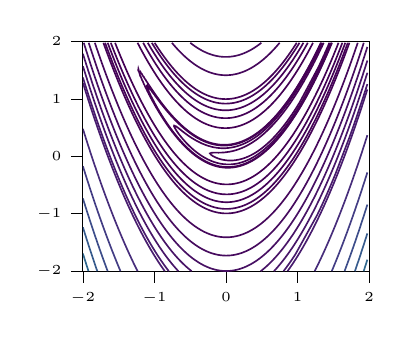
\begin{tikzpicture}

\definecolor{color0}{rgb}{0.267004,0.004874,0.329415}
\definecolor{color1}{rgb}{0.26851,0.009605,0.335427}
\definecolor{color2}{rgb}{0.269944,0.014625,0.341379}
\definecolor{color3}{rgb}{0.273809,0.031497,0.358853}
\definecolor{color4}{rgb}{0.276022,0.044167,0.370164}
\definecolor{color5}{rgb}{0.278791,0.062145,0.386592}
\definecolor{color6}{rgb}{0.280894,0.078907,0.402329}
\definecolor{color7}{rgb}{0.281924,0.089666,0.412415}
\definecolor{color8}{rgb}{0.28291,0.105393,0.426902}
\definecolor{color9}{rgb}{0.283091,0.110553,0.431554}
\definecolor{color10}{rgb}{0.278826,0.17549,0.483397}
\definecolor{color11}{rgb}{0.263663,0.237631,0.518762}
\definecolor{color12}{rgb}{0.239346,0.300855,0.540844}
\definecolor{color13}{rgb}{0.214298,0.355619,0.551184}
\definecolor{color14}{rgb}{0.190631,0.407061,0.556089}
\definecolor{color15}{rgb}{0.12156862745098,0.466666666666667,0.705882352941177}

\begin{axis}[
legend cell align={left},
legend style={
 fill opacity=0.8,
 draw opacity=1,
 text opacity=1,
 draw=white!80!black,
 nodes={scale=0.3, transform shape}
},
tick align=outside,
tick pos=left,
height=4.5cm,
ticklabel style = {font=\tiny},
x grid style={white!69.0196078431373!black},
xmin=-2, xmax=2,
xtick style={color=black},
y grid style={white!69.0196078431373!black},
ymin=-2, ymax=2,
ytick style={color=black}
]
% \addplot [draw=red, fill=red, mark=*, only marks,
% mark options={scale=0.6}]
% table{
% x  y
% -0.847316845794121 -0.259789935392427
% };
% \addlegendentry{$~$ search distribution mean}
\path [draw=color0, semithick]
(axis cs:1.443869508101,1.97499999999999)
--(axis cs:1.43485789897595,1.94999999999999)
--(axis cs:1.42747602316968,1.92499999999999)
--(axis cs:1.42499999999999,1.91637731481478)
--(axis cs:1.41792358471694,1.89999999999999)
--(axis cs:1.40897508686666,1.87499999999999)
--(axis cs:1.40156765210182,1.84999999999999)
--(axis cs:1.39999999999999,1.84469387755099)
--(axis cs:1.39145237633902,1.82499999999999)
--(axis cs:1.38265158753082,1.79999999999999)
--(axis cs:1.37526676192773,1.77499999999999)
--(axis cs:1.37499999999999,1.77412347560972)
--(axis cs:1.36448728509552,1.74999999999999)
--(axis cs:1.35589390114987,1.72499999999999)
--(axis cs:1.34999999999999,1.70559659090906)
--(axis cs:1.34745206453907,1.69999999999999)
--(axis cs:1.33706409704459,1.67499999999999)
--(axis cs:1.32871251066663,1.64999999999999)
--(axis cs:1.32499999999999,1.63820271164018)
--(axis cs:1.31899894784307,1.62499999999999)
--(axis cs:1.30921636865474,1.59999999999999)
--(axis cs:1.30111854589034,1.57499999999999)
--(axis cs:1.29999999999999,1.57156862745095)
%--(axis cs:1.29019580536445,1.54999999999999)
%--(axis cs:1.28097093536914,1.52499999999999)
%--(axis cs:1.27499999999999,1.5067973066298)
%--(axis cs:1.27179783323031,1.49999999999999)
%--(axis cs:1.26107762063013,1.47499999999999)
%--(axis cs:1.25234556581444,1.44999999999999)
%--(axis cs:1.24999999999999,1.44312499999997)
%--(axis cs:1.24148636350292,1.42499999999999)
%--(axis cs:1.23165924302693,1.39999999999999)
%--(axis cs:1.22499999999999,1.38069233425411)
%--(axis cs:1.22223934085809,1.37499999999999)
%--(axis cs:1.2110588297844,1.34999999999999)
%--(axis cs:1.20193930846023,1.32499999999999)
%--(axis cs:1.19999999999999,1.31960784313723)
%--(axis cs:1.19052553663952,1.29999999999999)
%--(axis cs:1.18047129909365,1.27499999999999)
%--(axis cs:1.17499999999999,1.26002810846558)
%--(axis cs:1.17001774389642,1.24999999999999)
%--(axis cs:1.15890344044569,1.22499999999999)
%--(axis cs:1.14999999999999,1.20105113636361)
%--(axis cs:1.14946312620161,1.19999999999999)
%--(axis cs:1.13717823629006,1.17499999999999)
%--(axis cs:1.12724024972108,1.14999999999999)
%--(axis cs:1.12499999999999,1.14424542682924)
%--(axis cs:1.11522015306912,1.12499999999999)
%--(axis cs:1.10454903155382,1.09999999999999)
%--(axis cs:1.09999999999999,1.0885714285714)
%--(axis cs:1.09293656852657,1.07499999999999)
%--(axis cs:1.08153530886833,1.04999999999999)
%--(axis cs:1.07499999999999,1.03396990740738)
%--(axis cs:1.07022194821208,1.02499999999999)
%--(axis cs:1.05812846383401,0.999999999999989)
%--(axis cs:1.04999999999999,0.980570652173889)
%--(axis cs:1.04696554786663,0.974999999999989)
--(axis cs:1.03425571101803,0.94999999999999)
--(axis cs:1.02499999999999,0.928482389502739)
--(axis cs:1.0230618441788,0.92499999999999)
--(axis cs:1.00984706280579,0.89999999999999)
--(axis cs:0.999999999999989,0.877777777777756)
--(axis cs:0.998421654894839,0.87499999999999)
--(axis cs:0.98484034993525,0.84999999999999)
--(axis cs:0.974999999999989,0.828482389502741)
--(axis cs:0.972981142651235,0.82499999999999)
--(axis cs:0.959185213732853,0.79999999999999)
--(axis cs:0.94999999999999,0.780570652173893)
--(axis cs:0.946706165896762,0.77499999999999)
--(axis cs:0.932845120569666,0.74999999999999)
--(axis cs:0.92499999999999,0.733969907407388)
--(axis cs:0.919590794878949,0.72499999999999)
--(axis cs:0.905796913919704,0.69999999999999)
--(axis cs:0.89999999999999,0.68857142857141)
--(axis cs:0.891650645427076,0.67499999999999)
--(axis cs:0.878028042480823,0.649999999999991)
--(axis cs:0.87499999999999,0.644245426829251)
--(axis cs:0.862913108413428,0.624999999999991)
--(axis cs:0.84999999999999,0.601051136363619)
--(axis cs:0.84931376640237,0.599999999999991)
--(axis cs:0.833406989267272,0.574999999999991)
--(axis cs:0.82499999999999,0.560028108465592)
--(axis cs:0.818321955516401,0.549999999999991)
--(axis cs:0.803153556710261,0.524999999999991)
--(axis cs:0.79999999999999,0.51960784313724)
--(axis cs:0.78665721552766,0.499999999999991)
--(axis cs:0.77499999999999,0.480692334254128)
--(axis cs:0.770978679806796,0.474999999999991)
--(axis cs:0.754334633723444,0.449999999999991)
--(axis cs:0.74999999999999,0.443124999999986)
--(axis cs:0.736903310301218,0.424999999999991)
--(axis cs:0.72499999999999,0.40679730662982)
--(axis cs:0.71989946623827,0.399999999999991)
--(axis cs:0.70234731944502,0.374999999999992)
--(axis cs:0.69999999999999,0.371568627450968)
--(axis cs:0.683407966061742,0.349999999999992)
--(axis cs:0.67499999999999,0.338202711640199)
--(axis cs:0.664445090678363,0.324999999999992)
--(axis cs:0.649999999999991,0.305596590909079)
--(axis cs:0.645344715543209,0.299999999999992)
--(axis cs:0.625684295710947,0.274999999999992)
--(axis cs:0.624999999999991,0.274123475609745)
--(axis cs:0.604343967002551,0.249999999999992)
--(axis cs:0.599999999999991,0.24469387755101)
--(axis cs:0.582421585928154,0.224999999999992)
--(axis cs:0.574999999999991,0.216377314814805)
--(axis cs:0.559738058551611,0.199999999999992)
--(axis cs:0.549999999999991,0.189266304347817)
--(axis cs:0.536095477719651,0.174999999999992)
--(axis cs:0.524999999999991,0.163427140883969)
--(axis cs:0.511285885589327,0.149999999999992)
--(axis cs:0.499999999999991,0.13888888888888)
--(axis cs:0.485100201147276,0.124999999999992)
--(axis cs:0.474999999999991,0.115637085635351)
--(axis cs:0.457334009518599,0.0999999999999925)
--(axis cs:0.449999999999991,0.0936141304347752)
--(axis cs:0.427786785569508,0.0749999999999926)
--(axis cs:0.424999999999991,0.0727265211640143)
--(axis cs:0.399999999999991,0.0535897435897373)
--(axis cs:0.395112904985263,0.0499999999999927)
--(axis cs:0.374999999999992,0.0360321969696912)
--(axis cs:0.358949630772611,0.0249999999999928)
--(axis cs:0.349999999999992,0.0192329545454491)
--(axis cs:0.324999999999992,0.00382760067113634)
--(axis cs:0.318430525557943,-7.105427357601e-15)
--(axis cs:0.299999999999992,-0.00975609756098002)
--(axis cs:0.274999999999992,-0.0228346631205709)
--(axis cs:0.270457504184474,-0.025000000000007)
--(axis cs:0.249999999999992,-0.0335937500000035)
--(axis cs:0.224999999999992,-0.0435793439716338)
--(axis cs:0.207661000718199,-0.0500000000000069)
--(axis cs:0.199999999999992,-0.0524390243902468)
--(axis cs:0.174999999999992,-0.0590918624161096)
--(axis cs:0.149999999999992,-0.0648161764705896)
--(axis cs:0.124999999999992,-0.0694375000000006)
--(axis cs:0.0999999999999926,-0.072758620689655)
--(axis cs:0.0749999999999926,-0.0745842889908248)
--(axis cs:0.0499999999999927,-0.0747596153846139)
--(axis cs:0.0249999999999928,-0.0732147277227704)
--(axis cs:-7.105427357601e-15,-0.069999999999998)
--(axis cs:-0.025000000000007,-0.0652939356435626)
--(axis cs:-0.0500000000000069,-0.0593749999999986)
--(axis cs:-0.0750000000000068,-0.0525659403669715)
--(axis cs:-0.0833271306289356,-0.0500000000000069)
--(axis cs:-0.100000000000007,-0.0426315789473646)
--(axis cs:-0.125000000000007,-0.0315257352941155)
--(axis cs:-0.1397572331227,-0.025000000000007)
--(axis cs:-0.150000000000007,-0.0181249999999944)
--(axis cs:-0.175000000000006,-0.0029664855072444)
--(axis cs:-0.180093312597192,-7.105427357601e-15)
--(axis cs:-0.200000000000006,0.0181818181818215)
--(axis cs:-0.209032743695891,0.0249999999999928)
--(axis cs:-0.224672320740168,0.0499999999999927)
--(axis cs:-0.200000000000006,0.0611111111111097)
--(axis cs:-0.175000000000006,0.0628370098039216)
--(axis cs:-0.150000000000007,0.0627343750000001)
--(axis cs:-0.125000000000007,0.0623958333333334)
--(axis cs:-0.100000000000007,0.0623809523809523)
--(axis cs:-0.0750000000000068,0.0629635989010987)
--(axis cs:-0.0500000000000069,0.0643229166666664)
--(axis cs:-0.025000000000007,0.0666130050505048)
--(axis cs:-7.105427357601e-15,0.0699999999999998)
--(axis cs:0.0249999999999928,0.074693813131313)
--(axis cs:0.0262519359834427,0.0749999999999926)
--(axis cs:0.0499999999999927,0.0792279411764684)
--(axis cs:0.0749999999999926,0.0849594465648834)
--(axis cs:0.0999999999999925,0.092258064516127)
--(axis cs:0.121058404167787,0.0999999999999925)
--(axis cs:0.124999999999992,0.101159274193545)
--(axis cs:0.149999999999992,0.109826388888886)
--(axis cs:0.174999999999992,0.120646469465646)
--(axis cs:0.183536014967243,0.124999999999992)
--(axis cs:0.199999999999992,0.132051282051278)
--(axis cs:0.224999999999992,0.144925809352514)
--(axis cs:0.233476040258361,0.149999999999992)
--(axis cs:0.249999999999992,0.158593749999995)
--(axis cs:0.274999999999992,0.174242356115103)
--(axis cs:0.276094582304782,0.174999999999992)
--(axis cs:0.299999999999992,0.189743589743584)
--(axis cs:0.314135836554379,0.199999999999992)
--(axis cs:0.324999999999992,0.207191154970754)
--(axis cs:0.348351385028265,0.224999999999992)
--(axis cs:0.349999999999992,0.226168478260863)
--(axis cs:0.374999999999992,0.245514112903219)
--(axis cs:0.380211749273859,0.249999999999992)
--(axis cs:0.399999999999991,0.266097560975602)
--(axis cs:0.40989243669009,0.274999999999992)
--(axis cs:0.424999999999991,0.288039108187127)
--(axis cs:0.437718616401079,0.299999999999992)
--(axis cs:0.449999999999991,0.311221590909083)
--(axis cs:0.464034580047738,0.324999999999992)
--(axis cs:0.474999999999991,0.335584846368706)
--(axis cs:0.489083714266213,0.349999999999992)
--(axis cs:0.499999999999991,0.361111111111102)
--(axis cs:0.513035260379318,0.374999999999992)
--(axis cs:0.524999999999991,0.387819483240214)
--(axis cs:0.53599987387273,0.399999999999991)
--(axis cs:0.549999999999991,0.415767045454535)
--(axis cs:0.558037094281291,0.424999999999991)
--(axis cs:0.574999999999991,0.445056652046773)
--(axis cs:0.5791556566091,0.449999999999991)
--(axis cs:0.599440922477904,0.474999999999991)
--(axis cs:0.599999999999991,0.475686274509793)
--(axis cs:0.619793485309516,0.499999999999991)
--(axis cs:0.624999999999991,0.506690705128193)
--(axis cs:0.639430606780168,0.524999999999991)
--(axis cs:0.649999999999991,0.539211956521727)
--(axis cs:0.658250636462819,0.549999999999991)
--(axis cs:0.67499999999999,0.573565423976595)
--(axis cs:0.676067446287728,0.574999999999991)
--(axis cs:0.69438226903664,0.599999999999991)
--(axis cs:0.69999999999999,0.608163265306109)
--(axis cs:0.712141838752696,0.624999999999991)
--(axis cs:0.72499999999999,0.644523393854734)
--(axis cs:0.72885627181983,0.649999999999991)
--(axis cs:0.745610009179065,0.67499999999999)
--(axis cs:0.74999999999999,0.681874999999985)
--(axis cs:0.762380993041022,0.69999999999999)
--(axis cs:0.77499999999999,0.720640712290487)
--(axis cs:0.777920194601669,0.72499999999999)
--(axis cs:0.79394329409092,0.74999999999999)
--(axis cs:0.79999999999999,0.760204081632637)
--(axis cs:0.809628553641828,0.77499999999999)
--(axis cs:0.824031404676559,0.79999999999999)
--(axis cs:0.82499999999999,0.801680983412306)
--(axis cs:0.839757432609749,0.82499999999999)
--(axis cs:0.84999999999999,0.843559782608678)
--(axis cs:0.854022573938128,0.84999999999999)
--(axis cs:0.868661257606485,0.87499999999999)
--(axis cs:0.87499999999999,0.886818910256392)
--(axis cs:0.883021885850266,0.89999999999999)
--(axis cs:0.896576501772421,0.92499999999999)
--(axis cs:0.89999999999999,0.931568627450962)
--(axis cs:0.910943355040559,0.94999999999999)
--(axis cs:0.923668497014426,0.974999999999989)
--(axis cs:0.92499999999999,0.977628850710882)
--(axis cs:0.937974574815318,0.999999999999989)
--(axis cs:0.94999999999999,1.02485795454543)
--(axis cs:0.950082294366946,1.02499999999999)
--(axis cs:0.964246791189306,1.04999999999999)
--(axis cs:0.974999999999989,1.07287534916199)
--(axis cs:0.976206527342661,1.07499999999999)
--(axis cs:0.989853188318477,1.09999999999999)
--(axis cs:0.999999999999989,1.1222222222222)
--(axis cs:1.00154900669945,1.12499999999999)
--(axis cs:1.01485930099371,1.14999999999999)
--(axis cs:1.02499999999999,1.17287534916199)
--(axis cs:1.02616584281718,1.17499999999999)
--(axis cs:1.03930873323762,1.19999999999999)
--(axis cs:1.04999999999999,1.22485795454543)
--(axis cs:1.05007687872381,1.22499999999999)
--(axis cs:1.0632256589974,1.24999999999999)
--(axis cs:1.07387984349362,1.27499999999999)
--(axis cs:1.07499999999999,1.27762885071088)
--(axis cs:1.08661458493525,1.29999999999999)
--(axis cs:1.09728421959313,1.32499999999999)
--(axis cs:1.09999999999999,1.33156862745096)
--(axis cs:1.10945703775898,1.34999999999999)
--(axis cs:1.12026357027256,1.37499999999999)
--(axis cs:1.12499999999999,1.38681891025639)
--(axis cs:1.13170377856746,1.39999999999999)
--(axis cs:1.14280162306009,1.42499999999999)
--(axis cs:1.14999999999999,1.44355978260867)
--(axis cs:1.15325918795338,1.44999999999999)
--(axis cs:1.16486024037013,1.47499999999999)
--(axis cs:1.17435462960856,1.49999999999999)
--(axis cs:1.17499999999999,1.5016809834123)
--(axis cs:1.18636823104693,1.52499999999999)
--(axis cs:1.19621077560686,1.54999999999999)
--(axis cs:1.19999999999999,1.56020408163263)
--(axis cs:1.20719982621109,1.57499999999999)
--(axis cs:1.21760748318035,1.59999999999999)
--(axis cs:1.22499999999999,1.62064071229047)
--(axis cs:1.22713076424207,1.62499999999999)
--(axis cs:1.23844614020474,1.64999999999999)
--(axis cs:1.24756297494295,1.67499999999999)
--(axis cs:1.24999999999999,1.68187499999997)
--(axis cs:1.25855381529658,1.69999999999999)
--(axis cs:1.26834075697305,1.72499999999999)
--(axis cs:1.27499999999999,1.74452339385472)
--(axis cs:1.27761268614451,1.74999999999999)
--(axis cs:1.28849883681417,1.77499999999999)
--(axis cs:1.29724713422371,1.79999999999999)
--(axis cs:1.29999999999999,1.80816326530609)
--(axis cs:1.30777957860615,1.82499999999999)
--(axis cs:1.31738514231723,1.84999999999999)
--(axis cs:1.32499999999999,1.87356542397658)
--(axis cs:1.32567688752457,1.87499999999999)
--(axis cs:1.33676004580193,1.89999999999999)
--(axis cs:1.34546331837008,1.92499999999999)
--(axis cs:1.34999999999999,1.93921195652171)
--(axis cs:1.35494288293335,1.94999999999999)
--(axis cs:1.36485543613974,1.97499999999999);

\path [draw=color0, semithick]
(axis cs:1.46209345824532,1.97499999999999)
--(axis cs:1.45423105482158,1.94999999999999)
--(axis cs:1.44999999999999,1.93570075757572)
--(axis cs:1.44570790998006,1.92499999999999)
--(axis cs:1.43651685393258,1.89999999999999)
--(axis cs:1.42857997326014,1.87499999999999)
--(axis cs:1.42499999999999,1.86317960037171)
--(axis cs:1.41965594558438,1.84999999999999)
--(axis cs:1.41048411765652,1.82499999999999)
--(axis cs:1.40251851643641,1.79999999999999)
--(axis cs:1.39999999999999,1.79188405797098)
--(axis cs:1.39308181936274,1.77499999999999)
--(axis cs:1.38399158793633,1.74999999999999)
--(axis cs:1.37603807556492,1.72499999999999)
--(axis cs:1.37499999999999,1.72173793859646)
--(axis cs:1.36600058104697,1.69999999999999)
--(axis cs:1.3570415249322,1.67499999999999)
--(axis cs:1.34999999999999,1.65306640624997)
--(axis cs:1.34869294648989,1.64999999999999)
--(axis cs:1.33843252601268,1.62499999999999)
--(axis cs:1.32964000184142,1.59999999999999)
--(axis cs:1.32499999999999,1.58594911710034)
--(axis cs:1.32029361829621,1.57499999999999)
--(axis cs:1.31039938424698,1.54999999999999)
%--(axis cs:1.30179466088386,1.52499999999999)
%--(axis cs:1.29999999999999,1.51971830985913)
%--(axis cs:1.29144760704808,1.49999999999999)
%--(axis cs:1.28192105306566,1.47499999999999)
%--(axis cs:1.27499999999999,1.45490541187736)
%--(axis cs:1.27281595837687,1.44999999999999)
%--(axis cs:1.26218691452789,1.42499999999999)
%--(axis cs:1.2530131468354,1.39999999999999)
%--(axis cs:1.24999999999999,1.39151785714283)
%--(axis cs:1.24258561609522,1.37499999999999)
%--(axis cs:1.23253290213236,1.34999999999999)
%--(axis cs:1.22499999999999,1.32913912835246)
%--(axis cs:1.22309540075368,1.32499999999999)
%--(axis cs:1.21204433822007,1.29999999999999)
%--(axis cs:1.20249601786623,1.27499999999999)
%--(axis cs:1.19999999999999,1.2683098591549)
%--(axis cs:1.19150587034201,1.24999999999999)
%--(axis cs:1.1811931064958,1.22499999999999)
%--(axis cs:1.17499999999999,1.20871863382897)
%--(axis cs:1.17085935603469,1.19999999999999)
%--(axis cs:1.15972835668113,1.17499999999999)
%--(axis cs:1.15001993587294,1.14999999999999)
%--(axis cs:1.14999999999999,1.1499493243243)
%--(axis cs:1.13804218025785,1.12499999999999)
%--(axis cs:1.12772328752623,1.09999999999999)
%--(axis cs:1.12499999999999,1.09322916666664)
%--(axis cs:1.11606432610238,1.07499999999999)
%--(axis cs:1.10513116924281,1.04999999999999)
%--(axis cs:1.09999999999999,1.03753623188403)
%--(axis cs:1.09371580357345,1.02499999999999)
--(axis cs:1.08218283764973,0.999999999999989)
--(axis cs:1.07499999999999,0.982975139405181)
--(axis cs:1.07091223055853,0.974999999999989)
--(axis cs:1.05881418468791,0.94999999999999)
--(axis cs:1.04999999999999,0.929640151515128)
--(axis cs:1.04756841922437,0.92499999999999)
--(axis cs:1.03496048399122,0.89999999999999)
--(axis cs:1.02499999999999,0.877606561302659)
--(axis cs:1.0236036636991,0.87499999999999)
--(axis cs:1.01055942979079,0.84999999999999)
--(axis cs:0.999999999999989,0.826923076923055)
--(axis cs:0.998946897296155,0.82499999999999)
--(axis cs:0.985554025686743,0.79999999999999)
--(axis cs:0.974999999999989,0.777606561302661)
--(axis cs:0.973540767353938,0.77499999999999)
--(axis cs:0.959894838576058,0.74999999999999)
--(axis cs:0.949999999999989,0.729640151515131)
--(axis cs:0.947343813524863,0.72499999999999)
--(axis cs:0.933541205268674,0.69999999999999)
--(axis cs:0.92499999999999,0.682975139405185)
--(axis cs:0.920330313171709,0.67499999999999)
--(axis cs:0.906461155588941,0.649999999999991)
--(axis cs:0.89999999999999,0.637536231884039)
--(axis cs:0.892487855184949,0.624999999999991)
--(axis cs:0.878630046793796,0.599999999999991)
--(axis cs:0.87499999999999,0.593229166666649)
--(axis cs:0.863813151024138,0.574999999999991)
--(axis cs:0.850028120825809,0.549999999999991)
--(axis cs:0.84999999999999,0.549949324324308)
--(axis cs:0.834306850479448,0.524999999999991)
--(axis cs:0.82499999999999,0.50871863382898)
--(axis cs:0.819332427125807,0.499999999999991)
--(axis cs:0.803968150372008,0.474999999999991)
--(axis cs:0.79999999999999,0.468309859154914)
--(axis cs:0.787787335231771,0.449999999999991)
--(axis cs:0.77499999999999,0.429139128352475)
--(axis cs:0.772143636183357,0.424999999999991)
--(axis cs:0.755407405299251,0.399999999999991)
--(axis cs:0.74999999999999,0.391517857142843)
--(axis cs:0.738284836779274,0.374999999999992)
--(axis cs:0.72499999999999,0.35490541187738)
--(axis cs:0.721395643452857,0.349999999999992)
--(axis cs:0.703638899839276,0.324999999999992)
--(axis cs:0.69999999999999,0.319718309859142)
--(axis cs:0.68507412960186,0.299999999999992)
--(axis cs:0.67499999999999,0.285949117100359)
--(axis cs:0.66639834994341,0.274999999999992)
--(axis cs:0.649999999999991,0.253066406249988)
--(axis cs:0.647496711444168,0.249999999999992)
--(axis cs:0.627549970857469,0.224999999999992)
--(axis cs:0.624999999999991,0.22173793859648)
--(axis cs:0.606638758196563,0.199999999999992)
--(axis cs:0.599999999999991,0.191884057971004)
--(axis cs:0.585139713795983,0.174999999999992)
--(axis cs:0.574999999999991,0.163179600371737)
--(axis cs:0.562892209178221,0.149999999999992)
--(axis cs:0.549999999999991,0.135700757575748)
--(axis cs:0.539719328572071,0.124999999999992)
--(axis cs:0.524999999999991,0.109503113026811)
--(axis cs:0.515431354583587,0.0999999999999925)
--(axis cs:0.499999999999991,0.084615384615376)
--(axis cs:0.489828612114115,0.0749999999999926)
--(axis cs:0.474999999999991,0.0610356800766202)
--(axis cs:0.462702140150496,0.0499999999999927)
--(axis cs:0.449999999999991,0.0387310606060531)
--(axis cs:0.433830499024246,0.0249999999999928)
--(axis cs:0.424999999999991,0.0176405669144911)
--(axis cs:0.40297104392734,-7.105427357601e-15)
--(axis cs:0.399999999999991,-0.0023188405797167)
--(axis cs:0.374999999999992,-0.0206313775510263)
--(axis cs:0.368755925034629,-0.025000000000007)
--(axis cs:0.349999999999992,-0.0375585937500055)
--(axis cs:0.330880918436246,-0.0500000000000069)
--(axis cs:0.324999999999992,-0.0536419609665479)
--(axis cs:0.299999999999992,-0.0680327868852504)
--(axis cs:0.287293282257298,-0.0750000000000068)
--(axis cs:0.274999999999992,-0.0813014846743337)
--(axis cs:0.249999999999992,-0.0932291666666702)
--(axis cs:0.234782863162807,-0.100000000000007)
--(axis cs:0.224999999999992,-0.10400263409962)
--(axis cs:0.199999999999992,-0.113114754098363)
--(axis cs:0.174999999999992,-0.12141784934498)
--(axis cs:0.162459392317957,-0.125000000000007)
--(axis cs:0.149999999999992,-0.128183593750002)
--(axis cs:0.124999999999992,-0.133386479591838)
--(axis cs:0.0999999999999925,-0.137457627118645)
--(axis cs:0.0749999999999926,-0.140304312227075)
--(axis cs:0.0499999999999927,-0.141852678571429)
--(axis cs:0.0249999999999928,-0.142057409502262)
--(axis cs:-7.105427357601e-15,-0.14090909090909)
--(axis cs:-0.025000000000007,-0.138437499999999)
--(axis cs:-0.0500000000000069,-0.13470982142857)
--(axis cs:-0.0750000000000068,-0.129823962882095)
--(axis cs:-0.0952370048087666,-0.125000000000007)
--(axis cs:-0.100000000000007,-0.123673469387752)
--(axis cs:-0.125000000000007,-0.115510670731705)
--(axis cs:-0.150000000000007,-0.106550925925924)
--(axis cs:-0.166762920183606,-0.100000000000007)
--(axis cs:-0.175000000000006,-0.0963210978835943)
--(axis cs:-0.200000000000006,-0.0843137254901932)
--(axis cs:-0.218772384833876,-0.0750000000000068)
--(axis cs:-0.225000000000006,-0.0715176104972333)
--(axis cs:-0.250000000000006,-0.0568749999999967)
--(axis cs:-0.261438078402817,-0.0500000000000069)
--(axis cs:-0.275000000000006,-0.0409927486187801)
--(axis cs:-0.299165188354366,-0.025000000000007)
--(axis cs:-0.300000000000006,-0.0243902439024334)
--(axis cs:-0.325000000000006,-0.00544808201057813)
--(axis cs:-0.332121552692998,-7.105427357601e-15)
--(axis cs:-0.350000000000006,0.0146875000000046)
--(axis cs:-0.362481733000937,0.0249999999999928)
--(axis cs:-0.375000000000006,0.0360321969697022)
--(axis cs:-0.390722264858864,0.0499999999999927)
--(axis cs:-0.400000000000006,0.0587179487179545)
--(axis cs:-0.417114461382962,0.0749999999999926)
--(axis cs:-0.425000000000006,0.082854446308731)
--(axis cs:-0.441897478296809,0.0999999999999925)
--(axis cs:-0.450000000000006,0.108506944444451)
--(axis cs:-0.465301602641533,0.124999999999992)
--(axis cs:-0.475000000000005,0.135675975177311)
--(axis cs:-0.487561222109921,0.149999999999992)
--(axis cs:-0.500000000000005,0.16428571428572)
--(axis cs:-0.508917292115622,0.174999999999992)
--(axis cs:-0.525000000000005,0.194186613475183)
--(axis cs:-0.52961049005132,0.199999999999992)
--(axis cs:-0.549814522860049,0.224999999999992)
--(axis cs:-0.550000000000005,0.225240384615394)
--(axis cs:-0.56778161415623,0.249999999999992)
--(axis cs:-0.575000000000005,0.259590022935787)
--(axis cs:-0.585658761005785,0.274999999999992)
--(axis cs:-0.600000000000005,0.294482758620695)
--(axis cs:-0.603690622071646,0.299999999999992)
--(axis cs:-0.620415954988438,0.324999999999992)
--(axis cs:-0.625000000000005,0.331709558823539)
--(axis cs:-0.635980400812214,0.349999999999992)
--(axis cs:-0.650000000000005,0.370677083333339)
--(axis cs:-0.652555222042635,0.374999999999992)
--(axis cs:-0.666588598194899,0.399999999999991)
--(axis cs:-0.675000000000005,0.413337862318848)
--(axis cs:-0.681087470449169,0.424999999999991)
--(axis cs:-0.694817813765175,0.449999999999991)
--(axis cs:-0.700000000000005,0.45909090909092)
--(axis cs:-0.70684847743671,0.474999999999991)
--(axis cs:-0.71769422173071,0.499999999999991)
--(axis cs:-0.725000000000005,0.515729166666675)
--(axis cs:-0.727674738107506,0.524999999999991)
--(axis cs:-0.725000000000005,0.535246710526313)
--(axis cs:-0.708483563096468,0.524999999999991)
--(axis cs:-0.700000000000005,0.522222222222232)
--(axis cs:-0.675619047619024,0.499999999999991)
--(axis cs:-0.675000000000005,0.499601715686284)
--(axis cs:-0.650000000000005,0.475144230769233)
--(axis cs:-0.649867739446705,0.474999999999991)
--(axis cs:-0.625000000000005,0.450475543478263)
--(axis cs:-0.624546491137135,0.449999999999991)
--(axis cs:-0.600000000000005,0.426129032258067)
--(axis cs:-0.598874711142363,0.424999999999991)
--(axis cs:-0.575000000000005,0.402325858778629)
--(axis cs:-0.572566150773832,0.399999999999991)
--(axis cs:-0.550000000000005,0.379227941176474)
--(axis cs:-0.545333265699495,0.374999999999992)
--(axis cs:-0.525000000000005,0.356976169064752)
--(axis cs:-0.516836788382607,0.349999999999992)
--(axis cs:-0.500000000000005,0.33571428571429)
--(axis cs:-0.48663250529129,0.324999999999992)
--(axis cs:-0.475000000000005,0.315609262589933)
--(axis cs:-0.454094905455847,0.299999999999992)
--(axis cs:-0.450000000000006,0.296875000000005)
--(axis cs:-0.425000000000006,0.278682383040939)
--(axis cs:-0.41955228722828,0.274999999999992)
--(axis cs:-0.400000000000006,0.261219512195126)
--(axis cs:-0.38185628004436,0.249999999999992)
--(axis cs:-0.375000000000006,0.24551411290323)
--(axis cs:-0.350000000000006,0.230516304347829)
--(axis cs:-0.339686269528755,0.224999999999992)
--(axis cs:-0.325000000000006,0.216547880116963)
--(axis cs:-0.300000000000006,0.204081632653063)
--(axis cs:-0.290827003009873,0.199999999999992)
--(axis cs:-0.275000000000006,0.192288756983243)
--(axis cs:-0.250000000000006,0.181875000000002)
--(axis cs:-0.230416592487071,0.174999999999992)
--(axis cs:-0.225000000000006,0.172875349162014)
--(axis cs:-0.200000000000006,0.164285714285716)
--(axis cs:-0.175000000000006,0.157368187203793)
--(axis cs:-0.150000000000007,0.151852678571429)
--(axis cs:-0.139470345702465,0.149999999999992)
--(axis cs:-0.125000000000007,0.147075320512822)
--(axis cs:-0.100000000000007,0.143333333333335)
--(axis cs:-0.0750000000000068,0.140898992890996)
--(axis cs:-0.0500000000000069,0.139699074074074)
--(axis cs:-0.025000000000007,0.139701769406393)
--(axis cs:-7.105427357601e-15,0.140909090909091)
--(axis cs:0.0249999999999928,0.143354737442922)
--(axis cs:0.0499999999999927,0.147106481481481)
--(axis cs:0.064144271569974,0.149999999999992)
--(axis cs:0.0749999999999926,0.151911105577687)
--(axis cs:0.0999999999999925,0.157540983606555)
--(axis cs:0.124999999999992,0.164594414893615)
--(axis cs:0.149999999999992,0.173281249999998)
--(axis cs:0.154250034497012,0.174999999999992)
--(axis cs:0.174999999999992,0.182488794820714)
--(axis cs:0.199999999999992,0.193220338983047)
--(axis cs:0.213583784357407,0.199999999999992)
--(axis cs:0.224999999999992,0.20519184362934)
--(axis cs:0.249999999999992,0.218229166666662)
--(axis cs:0.261380548017144,0.224999999999992)
--(axis cs:0.274999999999992,0.232508445945941)
--(axis cs:0.299999999999992,0.248305084745758)
--(axis cs:0.302451168134802,0.249999999999992)
--(axis cs:0.324999999999992,0.264660109561747)
--(axis cs:0.339073408798199,0.274999999999992)
--(axis cs:0.349999999999992,0.28263257575757)
--(axis cs:0.372301939563436,0.299999999999992)
--(axis cs:0.374999999999992,0.302017045454539)
--(axis cs:0.399999999999991,0.322295081967206)
--(axis cs:0.403090068473098,0.324999999999992)
--(axis cs:0.424999999999991,0.343644173306765)
--(axis cs:0.431911724884908,0.349999999999992)
--(axis cs:0.449999999999991,0.366308593749992)
--(axis cs:0.459015853720297,0.374999999999992)
--(axis cs:0.474999999999991,0.390230453667945)
--(axis cs:0.484686797147907,0.399999999999991)
--(axis cs:0.499999999999991,0.415384615384606)
--(axis cs:0.509131169246214,0.424999999999991)
--(axis cs:0.524999999999991,0.441774855212345)
--(axis cs:0.532495491929446,0.449999999999991)
--(axis cs:0.549999999999991,0.46943359374999)
--(axis cs:0.554877005347586,0.474999999999991)
--(axis cs:0.574999999999991,0.498425049800786)
--(axis cs:0.57632917244567,0.499999999999991)
--(axis cs:0.59727071462272,0.524999999999991)
--(axis cs:0.599999999999991,0.528309859154918)
--(axis cs:0.617671316383971,0.549999999999991)
--(axis cs:0.624999999999991,0.559289772727261)
--(axis cs:0.637364504704318,0.574999999999991)
--(axis cs:0.649999999999991,0.591723484848472)
--(axis cs:0.656304324304822,0.599999999999991)
--(axis cs:0.674487752995269,0.624999999999991)
--(axis cs:0.67499999999999,0.625703393470778)
--(axis cs:0.692908025961684,0.649999999999991)
--(axis cs:0.69999999999999,0.660144927536218)
--(axis cs:0.710627612351353,0.67499999999999)
--(axis cs:0.72499999999999,0.696408059845545)
--(axis cs:0.727499412298076,0.69999999999999)
--(axis cs:0.744492274690546,0.72499999999999)
--(axis cs:0.74999999999999,0.733482142857128)
--(axis cs:0.761150287797963,0.74999999999999)
--(axis cs:0.77499999999999,0.772180260617745)
--(axis cs:0.776857297262924,0.77499999999999)
--(axis cs:0.792985724854091,0.79999999999999)
--(axis cs:0.79999999999999,0.811594202898535)
--(axis cs:0.808580953761409,0.82499999999999)
--(axis cs:0.823378259226596,0.84999999999999)
--(axis cs:0.82499999999999,0.852765249140877)
--(axis cs:0.838842831546005,0.87499999999999)
--(axis cs:0.84999999999999,0.89475378787877)
--(axis cs:0.85320166440315,0.89999999999999)
--(axis cs:0.867913125825498,0.92499999999999)
--(axis cs:0.87499999999999,0.937926136363618)
--(axis cs:0.882180412510469,0.94999999999999)
--(axis cs:0.895988095517065,0.974999999999989)
--(axis cs:0.89999999999999,0.982535211267587)
--(axis cs:0.910130977608695,0.999999999999989)
--(axis cs:0.923214166685176,1.02499999999999)
--(axis cs:0.92499999999999,1.02845253436424)
--(axis cs:0.937203503223446,1.04999999999999)
--(axis cs:0.949702791635701,1.07499999999999)
--(axis cs:0.94999999999999,1.0755912162162)
--(axis cs:0.96351003903419,1.09999999999999)
--(axis cs:0.974999999999989,1.12372466216214)
--(axis cs:0.975698021501963,1.12499999999999)
--(axis cs:0.989134617561169,1.14999999999999)
--(axis cs:0.999999999999989,1.1730769230769)
--(axis cs:1.00103137972823,1.17499999999999)
--(axis cs:1.01413958420785,1.19999999999999)
--(axis cs:1.02499999999999,1.22372466216214)
--(axis cs:1.02567107702465,1.22499999999999)
--(axis cs:1.03856944172805,1.24999999999999)
--(axis cs:1.04973412841597,1.27499999999999)
--(axis cs:1.04999999999999,1.27559121621619)
--(axis cs:1.06245287083916,1.29999999999999)
--(axis cs:1.07348961758902,1.32499999999999)
--(axis cs:1.07499999999999,1.32845253436424)
--(axis cs:1.08580320031012,1.34999999999999)
--(axis cs:1.09679358717434,1.37499999999999)
--(axis cs:1.09999999999999,1.38253521126758)
--(axis cs:1.10861728234195,1.39999999999999)
--(axis cs:1.11965128745274,1.42499999999999)
--(axis cs:1.12499999999999,1.43792613636361)
--(axis cs:1.13087237194083,1.44999999999999)
--(axis cs:1.14205530059223,1.47499999999999)
--(axis cs:1.14999999999999,1.49475378787876)
--(axis cs:1.15252007187208,1.49999999999999)
--(axis cs:1.16398253156184,1.52499999999999)
--(axis cs:1.17390606148146,1.54999999999999)
--(axis cs:1.17499999999999,1.55276524914087)
--(axis cs:1.18538886101354,1.57499999999999)
--(axis cs:1.19554201131911,1.59999999999999)
--(axis cs:1.19999999999999,1.61159420289852)
--(axis cs:1.20619986175983,1.62499999999999)
--(axis cs:1.21671981694683,1.64999999999999)
--(axis cs:1.22499999999999,1.67218026061773)
--(axis cs:1.22629439262689,1.67499999999999)
--(axis cs:1.23737207154569,1.69999999999999)
--(axis cs:1.24688407104317,1.72499999999999)
--(axis cs:1.24999999999999,1.73348214285711)
--(axis cs:1.25739068773345,1.74999999999999)
--(axis cs:1.2673709646905,1.77499999999999)
--(axis cs:1.27499999999999,1.79640805984553)
--(axis cs:1.27660064090156,1.79999999999999)
--(axis cs:1.2872846520635,1.82499999999999)
--(axis cs:1.29644314591041,1.84999999999999)
--(axis cs:1.29999999999999,1.8601449275362)
--(axis cs:1.30646496501429,1.87499999999999)
--(axis cs:1.3162340407542,1.89999999999999)
--(axis cs:1.32475753313096,1.92499999999999)
--(axis cs:1.32499999999999,1.92570339347076)
--(axis cs:1.33534560020485,1.94999999999999)
--(axis cs:1.34441430898423,1.97499999999999);

\path [draw=color0, semithick]
(axis cs:1.47675005209304,1.97499999999999)
--(axis cs:1.47499999999999,1.96915047653955)
--(axis cs:1.4676807655127,1.94999999999999)
--(axis cs:1.45909124688804,1.92499999999999)
--(axis cs:1.4513984927356,1.89999999999999)
--(axis cs:1.44999999999999,1.89542151162787)
--(axis cs:1.4420906340159,1.87499999999999)
--(axis cs:1.4334278238116,1.84999999999999)
--(axis cs:1.42565256274104,1.82499999999999)
--(axis cs:1.42499999999999,1.82290920487103)
--(axis cs:1.41601056877433,1.79999999999999)
--(axis cs:1.40732233486713,1.77499999999999)
--(axis cs:1.39999999999999,1.7517721518987)
--(axis cs:1.39928624914366,1.74999999999999)
--(axis cs:1.38943710134409,1.72499999999999)
--(axis cs:1.38076669936791,1.69999999999999)
--(axis cs:1.37499999999999,1.68213942307689)
--(axis cs:1.3720901979841,1.67499999999999)
--(axis cs:1.36237295381517,1.64999999999999)
--(axis cs:1.35375709379193,1.62499999999999)
--(axis cs:1.34999999999999,1.6136458333333)
--(axis cs:1.34437138428959,1.59999999999999)
--(axis cs:1.33482509799666,1.57499999999999)
--(axis cs:1.32629273153718,1.54999999999999)
--(axis cs:1.32499999999999,1.54619000716329)
--(axis cs:1.31615194795483,1.52499999999999)
--(axis cs:1.30680263070484,1.49999999999999)
--(axis cs:1.29999999999999,1.48024691358022)
--(axis cs:1.29775662702274,1.47499999999999)
--(axis cs:1.28745334940388,1.44999999999999)
--(axis cs:1.27831472186555,1.42499999999999)
--(axis cs:1.27499999999999,1.41563141495598)
--(axis cs:1.26823746768796,1.39999999999999)
--(axis cs:1.25829385551822,1.37499999999999)
--(axis cs:1.24999999999999,1.35195312499997)
--(axis cs:1.24913529218477,1.34999999999999)
--(axis cs:1.23828772644996,1.32499999999999)
--(axis cs:1.22868672196353,1.29999999999999)
--(axis cs:1.22499999999999,1.29004490469205)
--(axis cs:1.21826034123191,1.27499999999999)
--(axis cs:1.20792344553359,1.24999999999999)
--(axis cs:1.19999999999999,1.22901234567898)
--(axis cs:1.19816173221387,1.22499999999999)
--(axis cs:1.18703544994156,1.19999999999999)
--(axis cs:1.17715081853012,1.17499999999999)
--(axis cs:1.17499999999999,1.16947080945556)
--(axis cs:1.16596863422657,1.14999999999999)
--(axis cs:1.15545887362677,1.12499999999999)
--(axis cs:1.14999999999999,1.11126488095236)
--(axis cs:1.14465838728456,1.09999999999999)
--(axis cs:1.13351024747135,1.07499999999999)
--(axis cs:1.12499999999999,1.05406249999997)
--(axis cs:1.12303059683403,1.04999999999999)
--(axis cs:1.1112455351999,1.02499999999999)
--(axis cs:1.10075435003609,0.999999999999989)
--(axis cs:1.09999999999999,0.998202247190988)
--(axis cs:1.08860041057843,0.974999999999989)
--(axis cs:1.07762410091333,0.94999999999999)
--(axis cs:1.07499999999999,0.943897743552986)
--(axis cs:1.06550778087613,0.92499999999999)
--(axis cs:1.05407149154444,0.89999999999999)
--(axis cs:1.04999999999999,0.890770348837187)
--(axis cs:1.04190041617677,0.87499999999999)
--(axis cs:1.03004084818092,0.84999999999999)
--(axis cs:1.02499999999999,0.838871884164201)
--(axis cs:1.01771376860427,0.82499999999999)
--(axis cs:1.00547785747299,0.79999999999999)
--(axis cs:0.999999999999989,0.788235294117626)
--(axis cs:0.992888607945001,0.77499999999999)
--(axis cs:0.980331208401378,0.74999999999999)
--(axis cs:0.974999999999989,0.738871884164202)
--(axis cs:0.967373077775758,0.72499999999999)
--(axis cs:0.95455384836043,0.69999999999999)
--(axis cs:0.94999999999999,0.69077034883719)
--(axis cs:0.941123836793123,0.67499999999999)
--(axis cs:0.928103652427356,0.649999999999991)
--(axis cs:0.92499999999999,0.64389774355299)
--(axis cs:0.914106084694315,0.624999999999991)
--(axis cs:0.900943378843987,0.599999999999991)
--(axis cs:0.89999999999999,0.598202247190993)
--(axis cs:0.886292447154972,0.574999999999991)
--(axis cs:0.87499999999999,0.554062499999982)
--(axis cs:0.872524781477745,0.549999999999991)
--(axis cs:0.857660863610892,0.524999999999991)
--(axis cs:0.84999999999999,0.511264880952364)
--(axis cs:0.842959285697672,0.499999999999991)
--(axis cs:0.828191742303631,0.474999999999991)
--(axis cs:0.82499999999999,0.469470809455571)
--(axis cs:0.812504309849437,0.449999999999991)
--(axis cs:0.79999999999999,0.429012345678996)
--(axis cs:0.797340357517321,0.424999999999991)
--(axis cs:0.781152164556096,0.399999999999991)
--(axis cs:0.77499999999999,0.390044904692067)
--(axis cs:0.764743733913081,0.374999999999992)
--(axis cs:0.74999999999999,0.351953124999985)
--(axis cs:0.748622703357844,0.349999999999992)
--(axis cs:0.731230041683928,0.324999999999992)
--(axis cs:0.72499999999999,0.315631414955998)
--(axis cs:0.713639875323009,0.299999999999992)
--(axis cs:0.69999999999999,0.280246913580233)
--(axis cs:0.69604823478134,0.274999999999992)
--(axis cs:0.677740564214859,0.249999999999992)
--(axis cs:0.67499999999999,0.246190007163311)
--(axis cs:0.658507791375123,0.224999999999992)
--(axis cs:0.649999999999991,0.213645833333321)
--(axis cs:0.638967425632382,0.199999999999992)
--(axis cs:0.624999999999991,0.182139423076911)
--(axis cs:0.618995244719044,0.174999999999992)
--(axis cs:0.599999999999991,0.151772151898723)
--(axis cs:0.598446978888613,0.149999999999992)
--(axis cs:0.576790259760167,0.124999999999992)
--(axis cs:0.574999999999991,0.12290920487105)
--(axis cs:0.554114285714279,0.0999999999999925)
--(axis cs:0.549999999999991,0.0954215116278973)
--(axis cs:0.530528704569857,0.0749999999999926)
--(axis cs:0.524999999999991,0.0691504765395803)
--(axis cs:0.50586144997618,0.0499999999999927)
--(axis cs:0.499999999999991,0.0441176470588149)
--(axis cs:0.479925105200162,0.0249999999999928)
--(axis cs:0.474999999999991,0.0203234970674406)
--(axis cs:0.452514498925246,-7.105427357601e-15)
--(axis cs:0.449999999999991,-0.00225290697675175)
--(axis cs:0.424999999999991,-0.0234779530744407)
--(axis cs:0.42310672772102,-0.025000000000007)
--(axis cs:0.399999999999991,-0.0431645569620319)
--(axis cs:0.390946717661226,-0.0500000000000069)
--(axis cs:0.374999999999992,-0.0617067307692368)
--(axis cs:0.356167928948936,-0.0750000000000068)
--(axis cs:0.349999999999992,-0.0792113095238152)
--(axis cs:0.324999999999992,-0.0952417071197461)
--(axis cs:0.317129474740705,-0.100000000000007)
--(axis cs:0.299999999999992,-0.109876543209881)
--(axis cs:0.274999999999992,-0.123653446843858)
--(axis cs:0.272319583367764,-0.125000000000007)
--(axis cs:0.249999999999992,-0.135546875000004)
--(axis cs:0.224999999999992,-0.146660091362129)
--(axis cs:0.216637204949551,-0.150000000000007)
--(axis cs:0.199999999999992,-0.156172839506176)
--(axis cs:0.174999999999992,-0.164416464401297)
--(axis cs:0.149999999999992,-0.171672297297299)
--(axis cs:0.136240614632415,-0.175000000000006)
--(axis cs:0.124999999999992,-0.177475961538463)
--(axis cs:0.0999999999999925,-0.181772151898735)
--(axis cs:0.0749999999999926,-0.184885720064726)
--(axis cs:0.0499999999999927,-0.186759868421053)
--(axis cs:0.0249999999999928,-0.187357765780731)
--(axis cs:-7.105427357601e-15,-0.186666666666666)
--(axis cs:-0.025000000000007,-0.18469995847176)
--(axis cs:-0.0500000000000069,-0.181496710526315)
--(axis cs:-0.0750000000000068,-0.177118729773462)
--(axis cs:-0.0845452888645616,-0.175000000000006)
--(axis cs:-0.100000000000007,-0.171159420289853)
--(axis cs:-0.125000000000007,-0.16378837719298)
--(axis cs:-0.150000000000007,-0.155456081081079)
--(axis cs:-0.164626967055344,-0.150000000000007)
--(axis cs:-0.175000000000006,-0.145742332713752)
--(axis cs:-0.200000000000006,-0.134507042253518)
--(axis cs:-0.219968567994809,-0.125000000000007)
--(axis cs:-0.225000000000006,-0.122393438697314)
--(axis cs:-0.250000000000006,-0.10848214285714)
--(axis cs:-0.264641288433371,-0.100000000000007)
--(axis cs:-0.275000000000006,-0.0935620210727927)
--(axis cs:-0.300000000000006,-0.0774647887323909)
--(axis cs:-0.303611738148975,-0.0750000000000068)
--(axis cs:-0.325000000000006,-0.0595899163568732)
--(axis cs:-0.337990180650837,-0.0500000000000069)
--(axis cs:-0.350000000000006,-0.0406835937499952)
--(axis cs:-0.369738216677924,-0.025000000000007)
--(axis cs:-0.375000000000006,-0.020631377551015)
--(axis cs:-0.399232935818293,-7.105427357601e-15)
--(axis cs:-0.400000000000006,0.000677966101700929)
--(axis cs:-0.425000000000006,0.0235885223048372)
--(axis cs:-0.426482068797261,0.0249999999999928)
--(axis cs:-0.450000000000006,0.0478219696969744)
--(axis cs:-0.452159928628439,0.0499999999999927)
--(axis cs:-0.475000000000005,0.0732962164751006)
--(axis cs:-0.47660081897133,0.0749999999999926)
--(axis cs:-0.499999999999992,0.0999999999999925)
--(axis cs:-0.500000000000005,0.100000000000007)
--(axis cs:-0.521981315881493,0.124999999999992)
--(axis cs:-0.525000000000005,0.128417703619916)
--(axis cs:-0.54308155238591,0.149999999999992)
--(axis cs:-0.550000000000005,0.158147321428578)
--(axis cs:-0.563491177127534,0.174999999999992)
--(axis cs:-0.575000000000005,0.189062500000006)
--(axis cs:-0.583388453970773,0.199999999999992)
--(axis cs:-0.600000000000005,0.221016949152548)
--(axis cs:-0.602933718253808,0.224999999999992)
--(axis cs:-0.621517063510333,0.249999999999992)
--(axis cs:-0.625000000000005,0.254611280487812)
--(axis cs:-0.639188271735896,0.274999999999992)
--(axis cs:-0.650000000000005,0.289745370370377)
--(axis cs:-0.65689145568389,0.299999999999992)
--(axis cs:-0.674644902901311,0.324999999999992)
--(axis cs:-0.675000000000005,0.325504298941807)
--(axis cs:-0.690578338590951,0.349999999999992)
--(axis cs:-0.700000000000005,0.363725490196085)
--(axis cs:-0.70696521179543,0.374999999999992)
--(axis cs:-0.723424989705808,0.399999999999991)
--(axis cs:-0.725000000000005,0.40237741712708)
--(axis cs:-0.738260535157668,0.424999999999991)
--(axis cs:-0.750000000000004,0.443125000000007)
--(axis cs:-0.753937430647524,0.449999999999991)
--(axis cs:-0.768649434011357,0.474999999999991)
--(axis cs:-0.775000000000004,0.485112223756914)
--(axis cs:-0.783121727009,0.499999999999991)
--(axis cs:-0.79813979444728,0.524999999999991)
--(axis cs:-0.800000000000004,0.528048780487814)
--(axis cs:-0.811399168810603,0.549999999999991)
--(axis cs:-0.825000000000004,0.572726521164027)
--(axis cs:-0.82616576796554,0.574999999999991)
--(axis cs:-0.838776060015745,0.599999999999991)
--(axis cs:-0.850000000000004,0.619232954545461)
--(axis cs:-0.85283193248003,0.624999999999991)
--(axis cs:-0.865255042543078,0.649999999999991)
--(axis cs:-0.875000000000004,0.66709280303031)
--(axis cs:-0.878721431882194,0.67499999999999)
--(axis cs:-0.890843653596811,0.69999999999999)
--(axis cs:-0.900000000000004,0.716410256410264)
--(axis cs:-0.903879419534611,0.72499999999999)
--(axis cs:-0.915564630844761,0.74999999999999)
--(axis cs:-0.925000000000004,0.767250419463094)
--(axis cs:-0.928364596612635,0.77499999999999)
--(axis cs:-0.939466324865993,0.79999999999999)
--(axis cs:-0.950000000000004,0.819618055555562)
--(axis cs:-0.952251516141915,0.82499999999999)
--(axis cs:-0.962630397155817,0.84999999999999)
--(axis cs:-0.975000000000004,0.873441932624119)
--(axis cs:-0.975629860588464,0.87499999999999)
--(axis cs:-0.985173516193296,0.89999999999999)
--(axis cs:-0.997379283233957,0.92499999999999)
--(axis cs:-1,0.93000000000001)
--(axis cs:-1.00724080191881,0.94999999999999)
--(axis cs:-1.01792917974002,0.974999999999989)
--(axis cs:-1.025,0.988666460396047)
--(axis cs:-1.02899141350303,0.999999999999989)
--(axis cs:-1.0381003496289,1.02499999999999)
--(axis cs:-1.05,1.04831730769231)
--(axis cs:-1.05057983019258,1.04999999999999)
--(axis cs:-1.05818679734794,1.07499999999999)
--(axis cs:-1.06801801801801,1.09999999999999)
--(axis cs:-1.075,1.11333786231885)
--(axis cs:-1.07843022326424,1.12499999999999)
--(axis cs:-1.08536461421191,1.14999999999999)
--(axis cs:-1.09570868578501,1.17499999999999)
--(axis cs:-1.1,1.18222222222224)
--(axis cs:-1.10380019297855,1.19999999999999)
--(axis cs:-1.10679993703762,1.22499999999999)
--(axis cs:-1.1,1.23727272727273)
--(axis cs:-1.09523862008156,1.22499999999999)
--(axis cs:-1.07576904874582,1.19999999999999)
--(axis cs:-1.075,1.19960171568629)
--(axis cs:-1.06481481481481,1.17499999999999)
--(axis cs:-1.05,1.15598958333334)
--(axis cs:-1.04727762324673,1.14999999999999)
--(axis cs:-1.03459588573656,1.12499999999999)
--(axis cs:-1.025,1.11257260101011)
--(axis cs:-1.01906691294762,1.09999999999999)
--(axis cs:-1.00388236435988,1.07499999999999)
--(axis cs:-1,1.07000000000001)
--(axis cs:-0.990206280222802,1.04999999999999)
--(axis cs:-0.975000000000004,1.02765962230216)
--(axis cs:-0.973639792116999,1.02499999999999)
--(axis cs:-0.960395944298267,0.999999999999989)
--(axis cs:-0.950000000000004,0.985110294117653)
--(axis cs:-0.944645899245554,0.974999999999989)
--(axis cs:-0.92923685115159,0.94999999999999)
--(axis cs:-0.925000000000004,0.944119751908405)
--(axis cs:-0.914502017079682,0.92499999999999)
--(axis cs:-0.900000000000004,0.903902439024395)
--(axis cs:-0.897780956095865,0.89999999999999)
--(axis cs:-0.882797677226463,0.87499999999999)
--(axis cs:-0.875000000000004,0.864062500000006)
--(axis cs:-0.866699195506254,0.84999999999999)
--(axis cs:-0.850000000000004,0.826168478260874)
--(axis cs:-0.849286691825981,0.82499999999999)
--(axis cs:-0.83372527062336,0.79999999999999)
--(axis cs:-0.825000000000004,0.788039108187141)
--(axis cs:-0.816716972370553,0.77499999999999)
--(axis cs:-0.800000000000004,0.752040816326535)
--(axis cs:-0.798658674602837,0.74999999999999)
--(axis cs:-0.781718658659715,0.72499999999999)
--(axis cs:-0.775000000000004,0.716171438547493)
--(axis cs:-0.763900206106498,0.69999999999999)
--(axis cs:-0.750000000000004,0.681875000000005)
--(axis cs:-0.745110459172328,0.67499999999999)
--(axis cs:-0.725811441750567,0.649999999999991)
--(axis cs:-0.725000000000005,0.648992667597773)
--(axis cs:-0.707089610592704,0.624999999999991)
--(axis cs:-0.700000000000005,0.616326530612251)
--(axis cs:-0.687342398022242,0.599999999999991)
--(axis cs:-0.675000000000005,0.585211789099532)
--(axis cs:-0.666763033401818,0.574999999999991)
--(axis cs:-0.650000000000005,0.555424107142862)
--(axis cs:-0.64543940318115,0.549999999999991)
--(axis cs:-0.625000000000005,0.526828457446813)
--(axis cs:-0.62339421684495,0.524999999999991)
--(axis cs:-0.600731972322287,0.499999999999991)
--(axis cs:-0.600000000000005,0.499215686274517)
--(axis cs:-0.5773822468952,0.474999999999991)
--(axis cs:-0.575000000000005,0.472534063981049)
--(axis cs:-0.552904443799003,0.449999999999991)
--(axis cs:-0.550000000000005,0.447106481481488)
--(axis cs:-0.527176315946695,0.424999999999991)
--(axis cs:-0.525000000000005,0.42292094748859)
--(axis cs:-0.500000000000005,0.400000000000004)
--(axis cs:-0.499999999999991,0.399999999999991)
--(axis cs:-0.475000000000005,0.377875241312745)
--(axis cs:-0.471532910434723,0.374999999999992)
--(axis cs:-0.450000000000006,0.356933593750004)
--(axis cs:-0.44107198994026,0.349999999999992)
--(axis cs:-0.425000000000006,0.337269671314745)
--(axis cs:-0.408040201005013,0.324999999999992)
--(axis cs:-0.400000000000006,0.319016393442628)
--(axis cs:-0.375000000000006,0.302017045454548)
--(axis cs:-0.371804565420885,0.299999999999992)
--(axis cs:-0.350000000000006,0.285662878787882)
--(axis cs:-0.3315303862872,0.274999999999992)
--(axis cs:-0.325000000000006,0.271034611553789)
--(axis cs:-0.300000000000006,0.257246376811597)
--(axis cs:-0.284986393919473,0.249999999999992)
--(axis cs:-0.275000000000006,0.244863658301162)
--(axis cs:-0.250000000000006,0.233482142857145)
--(axis cs:-0.228052443109602,0.224999999999992)
--(axis cs:-0.225000000000006,0.223724662162165)
--(axis cs:-0.200000000000006,0.214492753623191)
--(axis cs:-0.175000000000006,0.206888960481101)
--(axis cs:-0.150000000000007,0.200707236842106)
--(axis cs:-0.146499084062654,0.199999999999992)
--(axis cs:-0.125000000000007,0.195198863636365)
--(axis cs:-0.100000000000007,0.190985915492959)
--(axis cs:-0.0750000000000068,0.18807452749141)
--(axis cs:-0.0500000000000069,0.186402027027027)
--(axis cs:-0.025000000000007,0.185935409698997)
--(axis cs:-7.105427357601e-15,0.186666666666666)
--(axis cs:0.0249999999999928,0.188610994983277)
--(axis cs:0.0499999999999927,0.191807432432432)
--(axis cs:0.0749999999999926,0.19632195017182)
--(axis cs:0.0906449844691777,0.199999999999992)
--(axis cs:0.0999999999999925,0.201975308641973)
--(axis cs:0.124999999999992,0.208506944444442)
--(axis cs:0.149999999999992,0.216496710526313)
--(axis cs:0.172172188270591,0.224999999999992)
--(axis cs:0.174999999999992,0.225996034743199)
--(axis cs:0.199999999999992,0.236075949367085)
--(axis cs:0.224999999999992,0.247975543478257)
--(axis cs:0.228801915678715,0.249999999999992)
--(axis cs:0.249999999999992,0.260546874999996)
--(axis cs:0.274999999999992,0.274982232441467)
--(axis cs:0.275028226074237,0.274999999999992)
--(axis cs:0.299999999999992,0.289873417721514)
--(axis cs:0.315010260920539,0.299999999999992)
--(axis cs:0.324999999999992,0.306434101208453)
--(axis cs:0.349999999999992,0.324391447368415)
--(axis cs:0.350788618319379,0.324999999999992)
--(axis cs:0.374999999999992,0.343030753968247)
--(axis cs:0.383528383431253,0.349999999999992)
--(axis cs:0.399999999999991,0.363086419753079)
--(axis cs:0.41380605356104,0.374999999999992)
--(axis cs:0.424999999999991,0.384455249244705)
--(axis cs:0.442104716393093,0.399999999999991)
--(axis cs:0.449999999999991,0.407068452380944)
--(axis cs:0.468781903908342,0.424999999999991)
--(axis cs:0.474999999999991,0.430884033923295)
--(axis cs:0.494103990861177,0.449999999999991)
--(axis cs:0.499999999999991,0.455882352941167)
--(axis cs:0.51826933211537,0.474999999999991)
--(axis cs:0.524999999999991,0.482063974926244)
--(axis cs:0.541423844413673,0.499999999999991)
--(axis cs:0.549999999999991,0.509449404761895)
--(axis cs:0.563671300081758,0.524999999999991)
--(axis cs:0.574999999999991,0.538080626888207)
--(axis cs:0.58507967936639,0.549999999999991)
--(axis cs:0.599999999999991,0.568024691358013)
--(axis cs:0.60568428333385,0.574999999999991)
--(axis cs:0.624999999999991,0.599379960317448)
--(axis cs:0.625487778228695,0.599999999999991)
--(axis cs:0.64509317974136,0.624999999999991)
--(axis cs:0.649999999999991,0.63143895348836)
--(axis cs:0.66410776921589,0.649999999999991)
--(axis cs:0.67499999999999,0.664893315709957)
--(axis cs:0.682437126580513,0.67499999999999)
--(axis cs:0.69999999999999,0.699999999999986)
--(axis cs:0.699999999999993,0.69999999999999)
--(axis cs:0.717807568216485,0.72499999999999)
--(axis cs:0.72499999999999,0.735603797935089)
--(axis cs:0.73495550399061,0.74999999999999)
--(axis cs:0.74999999999999,0.773046874999985)
--(axis cs:0.751313611643847,0.77499999999999)
--(axis cs:0.767930745406695,0.79999999999999)
--(axis cs:0.77499999999999,0.811193768436563)
--(axis cs:0.784014252353317,0.82499999999999)
--(axis cs:0.799312965626805,0.84999999999999)
--(axis cs:0.79999999999999,0.851123595505602)
--(axis cs:0.815146452834385,0.87499999999999)
--(axis cs:0.82499999999999,0.891706004531705)
--(axis cs:0.830137066404691,0.89999999999999)
--(axis cs:0.844986801903845,0.92499999999999)
--(axis cs:0.84999999999999,0.933764534883704)
--(axis cs:0.859788156943495,0.94999999999999)
--(axis cs:0.873741864873838,0.974999999999989)
--(axis cs:0.87499999999999,0.977266725352095)
--(axis cs:0.888352325605437,0.999999999999989)
--(axis cs:0.89999999999999,1.02172839506171)
--(axis cs:0.901884151354228,1.02499999999999)
--(axis cs:0.915985210533556,1.04999999999999)
--(axis cs:0.92499999999999,1.06731023413895)
--(axis cs:0.929322789512785,1.07499999999999)
--(axis cs:0.942806703700211,1.09999999999999)
--(axis cs:0.94999999999999,1.11421130952379)
--(axis cs:0.955925259996317,1.12499999999999)
--(axis cs:0.968910041195573,1.14999999999999)
--(axis cs:0.974999999999989,1.16237370943951)
--(axis cs:0.981781095906682,1.17499999999999)
--(axis cs:0.994367882851957,1.19999999999999)
--(axis cs:0.999999999999989,1.21176470588233)
--(axis cs:1.00695746284521,1.22499999999999)
--(axis cs:1.01923638424677,1.24999999999999)
--(axis cs:1.02499999999999,1.26237370943951)
--(axis cs:1.03150293408283,1.27499999999999)
--(axis cs:1.04355785284246,1.29999999999999)
--(axis cs:1.04999999999999,1.31421130952379)
--(axis cs:1.05544959128065,1.32499999999999)
--(axis cs:1.06736232608514,1.34999999999999)
--(axis cs:1.07499999999999,1.36731023413895)
--(axis cs:1.07881370217069,1.37499999999999)
--(axis cs:1.09066823521614,1.39999999999999)
--(axis cs:1.09999999999999,1.4217283950617)
--(axis cs:1.10159497432618,1.42499999999999)
--(axis cs:1.11348217692039,1.44999999999999)
--(axis cs:1.12404498049163,1.47499999999999)
--(axis cs:1.12499999999999,1.47726672535209)
--(axis cs:1.13579766862341,1.49999999999999)
--(axis cs:1.14640391811906,1.52499999999999)
--(axis cs:1.14999999999999,1.5337645348837)
--(axis cs:1.15759257056434,1.54999999999999)
--(axis cs:1.16832636866957,1.57499999999999)
--(axis cs:1.17499999999999,1.5917060045317)
--(axis cs:1.17882455376578,1.59999999999999)
--(axis cs:1.18978854286812,1.62499999999999)
--(axis cs:1.19955938037865,1.64999999999999)
--(axis cs:1.19999999999999,1.65112359550559)
--(axis cs:1.2107487789071,1.67499999999999)
--(axis cs:1.22072568041338,1.69999999999999)
--(axis cs:1.22499999999999,1.71119376843655)
--(axis cs:1.23114042999819,1.72499999999999)
--(axis cs:1.24143649215495,1.74999999999999)
--(axis cs:1.24999999999999,1.77304687499997)
--(axis cs:1.25085994874705,1.77499999999999)
--(axis cs:1.26162738021533,1.79999999999999)
--(axis cs:1.27112969866627,1.82499999999999)
--(axis cs:1.27499999999999,1.83560379793507)
--(axis cs:1.28119948552646,1.84999999999999)
--(axis cs:1.29112571436595,1.87499999999999)
--(axis cs:1.29999999999999,1.89999999999997)
--(axis cs:1.3,1.89999999999999)
--(axis cs:1.31054268157251,1.92499999999999)
--(axis cs:1.31980641337986,1.94999999999999)
--(axis cs:1.32499999999999,1.96489331570994)
--(axis cs:1.32923236284851,1.97499999999999);

\path [draw=color0, semithick]
(axis cs:1.4802594781922,1.97499999999999)
--(axis cs:1.47499999999999,1.95742027126096)
--(axis cs:1.47216400240974,1.94999999999999)
--(axis cs:1.46305473326975,1.92499999999999)
--(axis cs:1.4549502203181,1.89999999999999)
--(axis cs:1.44999999999999,1.88379360465113)
--(axis cs:1.44659418760115,1.87499999999999)
--(axis cs:1.43741511432309,1.84999999999999)
--(axis cs:1.42922978033648,1.82499999999999)
--(axis cs:1.42499999999999,1.81144788681945)
--(axis cs:1.42050791955363,1.79999999999999)
--(axis cs:1.41131270809172,1.77499999999999)
--(axis cs:1.40308406082951,1.74999999999999)
--(axis cs:1.39999999999999,1.74033707865165)
--(axis cs:1.39390344327047,1.72499999999999)
--(axis cs:1.38474052181255,1.69999999999999)
--(axis cs:1.37650295838133,1.67499999999999)
--(axis cs:1.37499999999999,1.67039811643832)
--(axis cs:1.36678595562175,1.64999999999999)
--(axis cs:1.35769637955018,1.62499999999999)
--(axis cs:1.34999999999999,1.60174107142854)
--(axis cs:1.34928184510565,1.59999999999999)
--(axis cs:1.33916543464402,1.57499999999999)
--(axis cs:1.33018155966313,1.54999999999999)
--(axis cs:1.32499999999999,1.53472868911172)
--(axis cs:1.32093771031182,1.52499999999999)
--(axis cs:1.31105427489536,1.49999999999999)
--(axis cs:1.30219924699695,1.47499999999999)
--(axis cs:1.29999999999999,1.46868131868129)
--(axis cs:1.29210025703207,1.44999999999999)
--(axis cs:1.28246501433147,1.42499999999999)
--(axis cs:1.27499999999999,1.40390120967739)
--(axis cs:1.27331224130548,1.39999999999999)
--(axis cs:1.26279221783319,1.37499999999999)
--(axis cs:1.25340835931681,1.34999999999999)
--(axis cs:1.24999999999999,1.34062499999997)
--(axis cs:1.24315516480842,1.32499999999999)
--(axis cs:1.2330308295888,1.29999999999999)
--(axis cs:1.22499999999999,1.27831469941346)
--(axis cs:1.22351511568714,1.27499999999999)
--(axis cs:1.21258429584747,1.24999999999999)
--(axis cs:1.20282659617624,1.22499999999999)
--(axis cs:1.19999999999999,1.21758241758239)
--(axis cs:1.19202181534865,1.19999999999999)
--(axis cs:1.18160919540229,1.17499999999999)
--(axis cs:1.17499999999999,1.15800949140398)
--(axis cs:1.17128486701111,1.14999999999999)
--(axis cs:1.16019029172149,1.12499999999999)
--(axis cs:1.1502291103326,1.09999999999999)
--(axis cs:1.14999999999999,1.09942819148934)
--(axis cs:1.13851282692638,1.07499999999999)
--(axis cs:1.12800889862029,1.04999999999999)
--(axis cs:1.12499999999999,1.04265839041093)
--(axis cs:1.11651276480173,1.02499999999999)
--(axis cs:1.1054690377617,0.999999999999989)
--(axis cs:1.09999999999999,0.986966292134807)
--(axis cs:1.0941207928649,0.974999999999989)
--(axis cs:1.08255271304696,0.94999999999999)
--(axis cs:1.07499999999999,0.932436425501409)
--(axis cs:1.07126472969326,0.92499999999999)
--(axis cs:1.05920092971066,0.89999999999999)
--(axis cs:1.04999999999999,0.879142441860442)
--(axis cs:1.04787245954873,0.87499999999999)
--(axis cs:1.03535443269182,0.84999999999999)
--(axis cs:1.02499999999999,0.827141678885608)
--(axis cs:1.02387507942314,0.82499999999999)
--(axis cs:1.01095571494599,0.79999999999999)
--(axis cs:0.999999999999989,0.776470588235272)
--(axis cs:0.999209845327219,0.77499999999999)
--(axis cs:0.985950863143841,0.74999999999999)
--(axis cs:0.974999999999989,0.727141678885609)
--(axis cs:0.973822480198315,0.72499999999999)
--(axis cs:0.960290980153105,0.69999999999999)
--(axis cs:0.94999999999999,0.679142441860445)
--(axis cs:0.94766847325902,0.67499999999999)
--(axis cs:0.933932962929223,0.649999999999991)
--(axis cs:0.92499999999999,0.632436425501413)
--(axis cs:0.92071315012491,0.624999999999991)
--(axis cs:0.90683949661894,0.599999999999991)
--(axis cs:0.89999999999999,0.586966292134813)
--(axis cs:0.892930487273628,0.574999999999991)
--(axis cs:0.878978232226691,0.549999999999991)
--(axis cs:0.87499999999999,0.542658390410941)
--(axis cs:0.864300832071043,0.524999999999991)
--(axis cs:0.850320220430802,0.499999999999991)
--(axis cs:0.84999999999999,0.499428191489345)
--(axis cs:0.834807823516028,0.474999999999991)
--(axis cs:0.82499999999999,0.458009491403995)
--(axis cs:0.819859786231463,0.449999999999991)
--(axis cs:0.80443486295041,0.424999999999991)
--(axis cs:0.79999999999999,0.417582417582402)
--(axis cs:0.788401332034519,0.399999999999991)
--(axis cs:0.77499999999999,0.378314699413474)
--(axis cs:0.772740335357468,0.374999999999992)
--(axis cs:0.756013764839516,0.349999999999992)
--(axis cs:0.74999999999999,0.340624999999986)
--(axis cs:0.739030543841254,0.324999999999992)
--(axis cs:0.72499999999999,0.303901209677405)
--(axis cs:0.722164797399893,0.299999999999992)
--(axis cs:0.704370857780833,0.274999999999992)
--(axis cs:0.69999999999999,0.268681318681306)
--(axis cs:0.685984799690835,0.249999999999992)
--(axis cs:0.67499999999999,0.234728689111735)
--(axis cs:0.667428149304485,0.224999999999992)
--(axis cs:0.649999999999991,0.201741071428559)
--(axis cs:0.648592354197365,0.199999999999992)
--(axis cs:0.628599941061424,0.174999999999992)
--(axis cs:0.624999999999991,0.170398116438345)
--(axis cs:0.607900554072281,0.149999999999992)
--(axis cs:0.599999999999991,0.140337078651675)
--(axis cs:0.586604103413371,0.124999999999992)
--(axis cs:0.574999999999991,0.111447886819474)
--(axis cs:0.564563265306116,0.0999999999999925)
--(axis cs:0.549999999999991,0.083793604651153)
--(axis cs:0.541615563177764,0.0749999999999926)
--(axis cs:0.524999999999991,0.0574202712609878)
--(axis cs:0.517584349928557,0.0499999999999927)
--(axis cs:0.499999999999991,0.0323529411764619)
--(axis cs:0.492278886615443,0.0249999999999928)
--(axis cs:0.474999999999991,0.00859329178884814)
--(axis cs:0.465492557894302,-7.105427357601e-15)
--(axis cs:0.449999999999991,-0.013880813953496)
--(axis cs:0.436998087954103,-0.025000000000007)
--(axis cs:0.424999999999991,-0.0351137177650501)
--(axis cs:0.406538444454306,-0.0500000000000069)
--(axis cs:0.399999999999991,-0.0551685393258493)
--(axis cs:0.374999999999992,-0.0740144230769291)
--(axis cs:0.373603770500726,-0.0750000000000068)
--(axis cs:0.349999999999992,-0.091116071428577)
--(axis cs:0.336467954893172,-0.100000000000007)
--(axis cs:0.324999999999992,-0.107248388252154)
--(axis cs:0.299999999999992,-0.122222222222227)
--(axis cs:0.294994090245417,-0.125000000000007)
--(axis cs:0.274999999999992,-0.135541605571852)
--(axis cs:0.249999999999992,-0.148046875000004)
--(axis cs:0.245683329016648,-0.150000000000007)
--(axis cs:0.224999999999992,-0.158782074780062)
--(axis cs:0.199999999999992,-0.168518518518521)
--(axis cs:0.181446714522344,-0.175000000000006)
--(axis cs:0.174999999999992,-0.177090795128942)
--(axis cs:0.149999999999992,-0.183973214285716)
--(axis cs:0.124999999999992,-0.189783653846155)
--(axis cs:0.0999999999999925,-0.194430379746836)
--(axis cs:0.0749999999999926,-0.197830703883496)
--(axis cs:0.0499999999999927,-0.199917763157895)
--(axis cs:0.047155049786398,-0.200000000000006)
--(axis cs:0.0249999999999928,-0.200570931085044)
--(axis cs:2.70268558736718e-13,-0.200000000000006)
--(axis cs:-7.105427357601e-15,-0.199999999999999)
--(axis cs:-0.025000000000007,-0.19798899501661)
--(axis cs:-0.0500000000000069,-0.194654605263157)
--(axis cs:-0.0750000000000068,-0.190063713592231)
--(axis cs:-0.100000000000007,-0.184303797468353)
--(axis cs:-0.125000000000007,-0.17747596153846)
--(axis cs:-0.132768191142735,-0.175000000000006)
--(axis cs:-0.150000000000007,-0.168969594594592)
--(axis cs:-0.175000000000006,-0.159238470873784)
--(axis cs:-0.196927508401329,-0.150000000000007)
--(axis cs:-0.200000000000006,-0.148591549295771)
--(axis cs:-0.225000000000006,-0.136028862126243)
--(axis cs:-0.246038976471507,-0.125000000000007)
--(axis cs:-0.250000000000006,-0.122767857142853)
--(axis cs:-0.275000000000006,-0.10770660299003)
--(axis cs:-0.287287293915106,-0.100000000000007)
--(axis cs:-0.300000000000006,-0.0915492957746436)
--(axis cs:-0.324250241857455,-0.0750000000000068)
--(axis cs:-0.325000000000006,-0.0744598048327087)
--(axis cs:-0.350000000000006,-0.055456081081077)
--(axis cs:-0.35694885171838,-0.0500000000000069)
--(axis cs:-0.375000000000006,-0.0352796052631533)
--(axis cs:-0.387228048207849,-0.025000000000007)
--(axis cs:-0.400000000000006,-0.0139130434782558)
--(axis cs:-0.415520638609601,-7.105427357601e-15)
--(axis cs:-0.425000000000006,0.00871863382900179)
--(axis cs:-0.442095633081231,0.0249999999999928)
--(axis cs:-0.450000000000006,0.0326704545454603)
--(axis cs:-0.467185519087188,0.0499999999999927)
--(axis cs:-0.475000000000005,0.0579705459770175)
--(axis cs:-0.491000314988968,0.0749999999999926)
--(axis cs:-0.500000000000005,0.0846153846153906)
--(axis cs:-0.513735674121125,0.0999999999999925)
--(axis cs:-0.525000000000005,0.112568247126443)
--(axis cs:-0.535576335411313,0.124999999999992)
--(axis cs:-0.550000000000005,0.141761363636369)
--(axis cs:-0.556696170867803,0.149999999999992)
--(axis cs:-0.575000000000005,0.172101533457255)
--(axis cs:-0.577256121821531,0.174999999999992)
--(axis cs:-0.596784862058854,0.199999999999992)
--(axis cs:-0.600000000000005,0.204067796610177)
--(axis cs:-0.615417625716843,0.224999999999992)
--(axis cs:-0.625000000000005,0.237531887755109)
--(axis cs:-0.633839114551302,0.249999999999992)
--(axis cs:-0.650000000000005,0.271816406250006)
--(axis cs:-0.652176743564914,0.274999999999992)
--(axis cs:-0.669336522381668,0.299999999999992)
--(axis cs:-0.675000000000005,0.307948962882103)
--(axis cs:-0.686086956521734,0.324999999999992)
--(axis cs:-0.700000000000005,0.345081967213121)
--(axis cs:-0.703099073506145,0.349999999999992)
--(axis cs:-0.719078623613576,0.374999999999992)
--(axis cs:-0.725000000000005,0.383847567873311)
--(axis cs:-0.73470584236821,0.399999999999991)
--(axis cs:-0.750000000000004,0.423437500000006)
--(axis cs:-0.75091416034372,0.424999999999991)
--(axis cs:-0.765391774349424,0.449999999999991)
--(axis cs:-0.775000000000004,0.465182409502269)
--(axis cs:-0.780495836367662,0.474999999999991)
--(axis cs:-0.795177636288281,0.499999999999991)
--(axis cs:-0.800000000000004,0.50784313725491)
--(axis cs:-0.809190874774326,0.524999999999991)
--(axis cs:-0.824064911933498,0.549999999999991)
--(axis cs:-0.825000000000004,0.551562500000009)
--(axis cs:-0.837018007935695,0.574999999999991)
--(axis cs:-0.850000000000004,0.597152777777784)
--(axis cs:-0.851438891001078,0.599999999999991)
--(axis cs:-0.863992257524495,0.624999999999991)
--(axis cs:-0.875000000000004,0.644245426829275)
--(axis cs:-0.877798203219968,0.649999999999991)
--(axis cs:-0.890130851784499,0.67499999999999)
--(axis cs:-0.900000000000004,0.692653061224497)
--(axis cs:-0.903441579780715,0.69999999999999)
--(axis cs:-0.915459776354354,0.72499999999999)
--(axis cs:-0.925000000000004,0.742435515873023)
--(axis cs:-0.928418771484079,0.74999999999999)
--(axis cs:-0.940020032780909,0.77499999999999)
--(axis cs:-0.950000000000004,0.793614130434789)
--(axis cs:-0.952789565836718,0.79999999999999)
--(axis cs:-0.963872244616329,0.82499999999999)
--(axis cs:-0.975000000000004,0.846161947513819)
--(axis cs:-0.976623907898194,0.84999999999999)
--(axis cs:-0.987098161488007,0.87499999999999)
--(axis cs:-0.999999999999993,0.89999999999999)
--(axis cs:-1,0.90000000000001)
--(axis cs:-1.00979808937257,0.92499999999999)
--(axis cs:-1.02172240575643,0.94999999999999)
--(axis cs:-1.025,0.956420656028378)
--(axis cs:-1.03208430517527,0.974999999999989)
--(axis cs:-1.04293902279562,0.999999999999989)
--(axis cs:-1.05,1.01406250000001)
--(axis cs:-1.05407174018419,1.02499999999999)
--(axis cs:-1.06383309173742,1.04999999999999)
--(axis cs:-1.075,1.07261954697987)
--(axis cs:-1.07586808211215,1.07499999999999)
--(axis cs:-1.08457651494538,1.09999999999999)
--(axis cs:-1.09548143016997,1.12499999999999)
--(axis cs:-1.1,1.13413793103449)
--(axis cs:-1.10531158661999,1.14999999999999)
--(axis cs:-1.11452920895449,1.17499999999999)
--(axis cs:-1.125,1.19656250000001)
--(axis cs:-1.12614100308693,1.19999999999999)
--(axis cs:-1.13394537576049,1.22499999999999)
--(axis cs:-1.14391019464251,1.24999999999999)
--(axis cs:-1.15,1.26234375000001)
--(axis cs:-1.15380385864673,1.27499999999999)
--(axis cs:-1.16154971567382,1.29999999999999)
--(axis cs:-1.17259908179518,1.32499999999999)
--(axis cs:-1.175,1.32964221014494)
--(axis cs:-1.18031700969955,1.34999999999999)
--(axis cs:-1.18758773550055,1.37499999999999)
--(axis cs:-1.19999999999999,1.39999999999999)
--(axis cs:-1.2,1.40000000000002)
--(axis cs:-1.20520802509321,1.42499999999999)
--(axis cs:-1.21050673087446,1.44999999999999)
--(axis cs:-1.21742919389977,1.47499999999999)
--(axis cs:-1.2,1.47894736842105)
--(axis cs:-1.19857693447969,1.47499999999999)
--(axis cs:-1.189638424177,1.44999999999999)
--(axis cs:-1.175,1.4313701923077)
--(axis cs:-1.17257033583067,1.42499999999999)
--(axis cs:-1.16226066798317,1.39999999999999)
--(axis cs:-1.15,1.38283653846154)
--(axis cs:-1.1468703499256,1.37499999999999)
--(axis cs:-1.13574485353796,1.34999999999999)
--(axis cs:-1.125,1.33417119565218)
--(axis cs:-1.12118678537533,1.32499999999999)
--(axis cs:-1.10938228826547,1.29999999999999)
--(axis cs:-1.1,1.28580645161291)
--(axis cs:-1.0953377114774,1.27499999999999)
--(axis cs:-1.0828354019834,1.24999999999999)
--(axis cs:-1.075,1.2380128816794)
--(axis cs:-1.06918567469622,1.22499999999999)
--(axis cs:-1.05588411888321,1.19999999999999)
--(axis cs:-1.05,1.19099264705883)
--(axis cs:-1.04260738411862,1.17499999999999)
--(axis cs:-1.0283393501805,1.14999999999999)
--(axis cs:-1.025,1.14492580935253)
--(axis cs:-1.01547521815758,1.12499999999999)
--(axis cs:-1,1.1)
--(axis cs:-0.999999999999996,1.09999999999999)
--(axis cs:-0.987641788409757,1.07499999999999)
--(axis cs:-0.975000000000004,1.05499825418995)
--(axis cs:-0.97243486363473,1.04999999999999)
--(axis cs:-0.958922411810691,1.02499999999999)
--(axis cs:-0.950000000000004,1.0112215909091)
--(axis cs:-0.944047843284983,0.999999999999989)
--(axis cs:-0.929070333414448,0.974999999999989)
--(axis cs:-0.925000000000004,0.968887061403516)
--(axis cs:-0.914634733421585,0.94999999999999)
--(axis cs:-0.900000000000004,0.927647058823534)
--(axis cs:-0.898497548081934,0.92499999999999)
--(axis cs:-0.883911931695048,0.89999999999999)
--(axis cs:-0.875000000000004,0.886818910256417)
--(axis cs:-0.868049534436606,0.87499999999999)
--(axis cs:-0.851466177940678,0.84999999999999)
--(axis cs:-0.850000000000004,0.84790760869566)
--(axis cs:-0.836015842076881,0.82499999999999)
--(axis cs:-0.825000000000004,0.809263921800954)
--(axis cs:-0.819150925752753,0.79999999999999)
--(axis cs:-0.801857441374498,0.77499999999999)
--(axis cs:-0.800000000000004,0.772448979591844)
--(axis cs:-0.785245420631254,0.74999999999999)
--(axis cs:-0.775000000000004,0.736048801369869)
--(axis cs:-0.767480480130515,0.72499999999999)
--(axis cs:-0.750000000000004,0.701562500000005)
--(axis cs:-0.748897747731192,0.69999999999999)
--(axis cs:-0.730886340400934,0.67499999999999)
--(axis cs:-0.725000000000005,0.667441495433796)
--(axis cs:-0.71212989091521,0.649999999999991)
--(axis cs:-0.700000000000005,0.63474576271187)
--(axis cs:-0.692527918781719,0.624999999999991)
--(axis cs:-0.675000000000005,0.603504731075702)
--(axis cs:-0.672203679421458,0.599999999999991)
--(axis cs:-0.651471782864233,0.574999999999991)
--(axis cs:-0.650000000000005,0.573281250000007)
--(axis cs:-0.630425092666439,0.549999999999991)
--(axis cs:-0.625000000000005,0.543849734042559)
--(axis cs:-0.608445835474369,0.524999999999991)
--(axis cs:-0.600000000000005,0.515737704918038)
--(axis cs:-0.585531954975737,0.499999999999991)
--(axis cs:-0.575000000000005,0.488863296812754)
--(axis cs:-0.561626231083345,0.474999999999991)
--(axis cs:-0.550000000000005,0.463183593750005)
--(axis cs:-0.536618426921734,0.449999999999991)
--(axis cs:-0.525000000000005,0.438686052123557)
--(axis cs:-0.510339657757319,0.424999999999991)
--(axis cs:-0.500000000000005,0.41538461538462)
--(axis cs:-0.482548944756493,0.399999999999991)
--(axis cs:-0.475000000000005,0.393319256756762)
--(axis cs:-0.452909852761439,0.374999999999992)
--(axis cs:-0.450000000000006,0.372558593750005)
--(axis cs:-0.425000000000006,0.352765249140897)
--(axis cs:-0.42125007281411,0.349999999999992)
--(axis cs:-0.400000000000006,0.333943661971835)
--(axis cs:-0.386934996463693,0.324999999999992)
--(axis cs:-0.375000000000006,0.316562500000004)
--(axis cs:-0.350000000000006,0.300707236842108)
--(axis cs:-0.348801644255543,0.299999999999992)
--(axis cs:-0.325000000000006,0.285325386597941)
--(axis cs:-0.305762304921954,0.274999999999992)
--(axis cs:-0.300000000000006,0.271739130434786)
--(axis cs:-0.275000000000006,0.258928720735789)
--(axis cs:-0.254742483164167,0.249999999999992)
--(axis cs:-0.250000000000006,0.24776785714286)
--(axis cs:-0.225000000000006,0.23727320234114)
--(axis cs:-0.200000000000006,0.22848101265823)
--(axis cs:-0.188398154251788,0.224999999999992)
--(axis cs:-0.175000000000006,0.220634664948456)
--(axis cs:-0.150000000000007,0.213865131578949)
--(axis cs:-0.125000000000007,0.208506944444446)
--(axis cs:-0.100000000000007,0.204444444444445)
--(axis cs:-0.0750000000000068,0.201600264350453)
--(axis cs:-0.0511267605632711,0.199999999999992)
--(axis cs:-0.0500000000000069,0.199915540540541)
--(axis cs:-0.025000000000007,0.199313336120402)
--(axis cs:-2.97811775240574e-13,0.199999999999992)
--(axis cs:-7.105427357601e-15,0.199999999999999)
--(axis cs:0.0249999999999928,0.201754240412978)
--(axis cs:0.0499999999999927,0.204687499999999)
--(axis cs:0.0749999999999926,0.208851019637461)
--(axis cs:0.0999999999999925,0.214320987654319)
--(axis cs:0.124999999999992,0.221205357142855)
--(axis cs:0.13644798276066,0.224999999999992)
--(axis cs:0.149999999999992,0.22911337209302)
--(axis cs:0.174999999999992,0.238080626888215)
--(axis cs:0.199999999999992,0.248734177215187)
--(axis cs:0.202635263114534,0.249999999999992)
--(axis cs:0.224999999999992,0.260013827433624)
--(axis cs:0.249999999999992,0.273046874999996)
--(axis cs:0.25338226341066,0.274999999999992)
--(axis cs:0.274999999999992,0.286783738938048)
--(axis cs:0.296212345386742,0.299999999999992)
--(axis cs:0.299999999999992,0.302247191011231)
--(axis cs:0.324999999999992,0.318518693353469)
--(axis cs:0.333998322235609,0.324999999999992)
--(axis cs:0.349999999999992,0.336090116279064)
--(axis cs:0.368153364632227,0.349999999999992)
--(axis cs:0.374999999999992,0.355083626760557)
--(axis cs:0.399514584145961,0.374999999999992)
--(axis cs:0.399999999999991,0.375384615384608)
--(axis cs:0.424999999999991,0.396539841389721)
--(axis cs:0.428807396634106,0.399999999999991)
--(axis cs:0.449999999999991,0.418973214285706)
--(axis cs:0.456312590110266,0.424999999999991)
--(axis cs:0.474999999999991,0.442683443952794)
--(axis cs:0.482311972583549,0.449999999999991)
--(axis cs:0.499999999999991,0.46764705882352)
--(axis cs:0.507026666198214,0.474999999999991)
--(axis cs:0.524999999999991,0.493863384955743)
--(axis cs:0.530619238950594,0.499999999999991)
--(axis cs:0.549999999999991,0.521354166666657)
--(axis cs:0.553205233033516,0.524999999999991)
--(axis cs:0.574871982443299,0.549999999999991)
--(axis cs:0.574999999999991,0.550147405660367)
--(axis cs:0.596031135061151,0.574999999999991)
--(axis cs:0.599999999999991,0.579780219780209)
--(axis cs:0.616480532930269,0.599999999999991)
--(axis cs:0.624999999999991,0.610717429577453)
--(axis cs:0.636232104782204,0.624999999999991)
--(axis cs:0.649999999999991,0.643066860465104)
--(axis cs:0.655269699229424,0.649999999999991)
--(axis cs:0.673705095557142,0.67499999999999)
--(axis cs:0.67499999999999,0.676764656334219)
--(axis cs:0.692076265940317,0.69999999999999)
--(axis cs:0.69999999999999,0.711235955056166)
--(axis cs:0.709804166770871,0.72499999999999)
--(axis cs:0.72499999999999,0.747403207964587)
--(axis cs:0.726795777341453,0.74999999999999)
--(axis cs:0.743854837608387,0.77499999999999)
--(axis cs:0.74999999999999,0.784374999999985)
--(axis cs:0.760479007055858,0.79999999999999)
--(axis cs:0.77499999999999,0.822993178466061)
--(axis cs:0.776310277583835,0.82499999999999)
--(axis cs:0.79244262189492,0.84999999999999)
--(axis cs:0.79999999999999,0.862359550561782)
--(axis cs:0.808018710324083,0.87499999999999)
--(axis cs:0.822996307016662,0.89999999999999)
--(axis cs:0.82499999999999,0.90338190700807)
--(axis cs:0.838335792821061,0.92499999999999)
--(axis cs:0.84999999999999,0.945392441860448)
--(axis cs:0.852777838631229,0.94999999999999)
--(axis cs:0.867487833955473,0.974999999999989)
--(axis cs:0.87499999999999,0.988534330985898)
--(axis cs:0.881734328790348,0.999999999999989)
--(axis cs:0.895647104547215,1.02499999999999)
--(axis cs:0.89999999999999,1.0330769230769)
--(axis cs:0.909691820559713,1.04999999999999)
--(axis cs:0.92294706017252,1.07499999999999)
--(axis cs:0.92499999999999,1.07892099056602)
--(axis cs:0.936780905752748,1.09999999999999)
--(axis cs:0.949492428728528,1.12499999999999)
--(axis cs:0.94999999999999,1.12599734042551)
--(axis cs:0.963102734878313,1.14999999999999)
--(axis cs:0.974999999999989,1.17417311946901)
--(axis cs:0.975444085787269,1.17499999999999)
--(axis cs:0.988735765703921,1.19999999999999)
--(axis cs:0.999999999999989,1.22352941176468)
--(axis cs:1.00077305142724,1.22499999999999)
--(axis cs:1.01374027446198,1.24999999999999)
--(axis cs:1.02499999999999,1.274173119469)
--(axis cs:1.02542586930512,1.27499999999999)
--(axis cs:1.03816128977857,1.29999999999999)
--(axis cs:1.04954502024659,1.32499999999999)
--(axis cs:1.04999999999999,1.32599734042551)
--(axis cs:1.06203032575189,1.34999999999999)
--(axis cs:1.07325825039287,1.37499999999999)
--(axis cs:1.07499999999999,1.37892099056601)
--(axis cs:1.0853660961344,1.39999999999999)
--(axis cs:1.09650587553667,1.42499999999999)
--(axis cs:1.09999999999999,1.4330769230769)
--(axis cs:1.10817423325094,1.44999999999999)
--(axis cs:1.11929769905202,1.47499999999999)
--(axis cs:1.12499999999999,1.48853433098589)
--(axis cs:1.13044587159031,1.49999999999999)
--(axis cs:1.14163299688399,1.52499999999999)
--(axis cs:1.14999999999999,1.54539244186044)
--(axis cs:1.15215474025863,1.54999999999999)
--(axis cs:1.16349887609938,1.57499999999999)
--(axis cs:1.17363855846568,1.59999999999999)
--(axis cs:1.17499999999999,1.60338190700806)
--(axis cs:1.18486735870818,1.62499999999999)
--(axis cs:1.19515318416523,1.64999999999999)
--(axis cs:1.19999999999999,1.66235955056177)
--(axis cs:1.20569053000964,1.67499999999999)
--(axis cs:1.21622009771482,1.69999999999999)
--(axis cs:1.22499999999999,1.72299317846605)
--(axis cs:1.22589254964986,1.72499999999999)
--(axis cs:1.23679187773052,1.74999999999999)
--(axis cs:1.24648515302602,1.77499999999999)
--(axis cs:1.24999999999999,1.78437499999997)
--(axis cs:1.25679522220376,1.79999999999999)
--(axis cs:1.26682300849225,1.82499999999999)
--(axis cs:1.27499999999999,1.84740320796457)
--(axis cs:1.27611826539847,1.84999999999999)
--(axis cs:1.28663240518415,1.87499999999999)
--(axis cs:1.29597266446002,1.89999999999999)
--(axis cs:1.29999999999999,1.91123595505615)
--(axis cs:1.3058043977197,1.92499999999999)
--(axis cs:1.3155922828735,1.94999999999999)
--(axis cs:1.32437896484259,1.97499999999999);

\path [draw=color0, semithick]
(axis cs:-1.225,1.48120535714288)
--(axis cs:-1.22745471507424,1.49999999999999)
--(axis cs:-1.225,1.5207730263158)
--(axis cs:-1.22005326648911,1.49999999999999)
--(axis cs:-1.225,1.48120535714288);

\path [draw=color0, semithick]
(axis cs:-1.23641156252497,1.97499999999999)
--(axis cs:-1.22571262249704,1.94999999999999)
--(axis cs:-1.225,1.94834719241775)
--(axis cs:-1.21556003846626,1.92499999999999)
--(axis cs:-1.20490259914357,1.89999999999999)
--(axis cs:-1.2,1.88882681564247)
--(axis cs:-1.19428014299642,1.87499999999999)
--(axis cs:-1.18361670423718,1.84999999999999)
--(axis cs:-1.175,1.83071776675787)
--(axis cs:-1.17257922057237,1.82499999999999)
--(axis cs:-1.161866520771,1.79999999999999)
--(axis cs:-1.15050954587129,1.77499999999999)
--(axis cs:-1.15,1.77388494318183)
--(axis cs:-1.13965493374758,1.74999999999999)
--(axis cs:-1.12822293548833,1.72499999999999)
--(axis cs:-1.125,1.71808347902099)
--(axis cs:-1.11697704902774,1.69999999999999)
--(axis cs:-1.10542497557611,1.67499999999999)
--(axis cs:-1.1,1.663591160221)
--(axis cs:-1.09382069658458,1.64999999999999)
--(axis cs:-1.08210457266695,1.62499999999999)
--(axis cs:-1.075,1.61036892954857)
--(axis cs:-1.07016659359929,1.59999999999999)
--(axis cs:-1.05824238338038,1.57499999999999)
--(axis cs:-1.05,1.55838994565218)
--(axis cs:-1.04598820825584,1.54999999999999)
--(axis cs:-1.03381074190751,1.52499999999999)
--(axis cs:-1.025,1.50763827807849)
--(axis cs:-1.02125133858529,1.49999999999999)
--(axis cs:-1.00877323811445,1.47499999999999)
--(axis cs:-1,1.45810810810811)
--(axis cs:-0.995913398094616,1.44999999999999)
--(axis cs:-0.983083941441638,1.42499999999999)
--(axis cs:-0.975000000000004,1.40980336603519)
--(axis cs:-0.969922378069608,1.39999999999999)
--(axis cs:-0.956686237648512,1.37499999999999)
--(axis cs:-0.950000000000004,1.36273777173914)
--(axis cs:-0.94321543262924,1.34999999999999)
--(axis cs:-0.929511215266147,1.32499999999999)
--(axis cs:-0.925000000000004,1.31693527701779)
--(axis cs:-0.915717003946116,1.29999999999999)
--(axis cs:-0.90147550249387,1.27499999999999)
--(axis cs:-0.900000000000004,1.27243093922653)
--(axis cs:-0.887336367978315,1.24999999999999)
--(axis cs:-0.875000000000004,1.22904594370862)
--(axis cs:-0.872645871665681,1.22499999999999)
--(axis cs:-0.857964430697847,1.19999999999999)
--(axis cs:-0.850000000000004,1.18684811827958)
--(axis cs:-0.842887759321446,1.17499999999999)
--(axis cs:-0.827469533973743,1.14999999999999)
--(axis cs:-0.825000000000004,1.14603924418605)
--(axis cs:-0.811957385911903,1.12499999999999)
--(axis cs:-0.800000000000004,1.10634920634921)
--(axis cs:-0.795932935806045,1.09999999999999)
--(axis cs:-0.779681573559186,1.07499999999999)
--(axis cs:-0.775000000000004,1.06792244587281)
--(axis cs:-0.763119092203664,1.04999999999999)
--(axis cs:-0.750000000000004,1.03075657894737)
--(axis cs:-0.746048635650331,1.02499999999999)
--(axis cs:-0.728654137400567,0.999999999999989)
--(axis cs:-0.725000000000005,0.994816897834919)
--(axis cs:-0.710888548956306,0.974999999999989)
--(axis cs:-0.700000000000005,0.960052910052916)
--(axis cs:-0.69256950809654,0.94999999999999)
--(axis cs:-0.675000000000005,0.926692201686128)
--(axis cs:-0.673699976334891,0.92499999999999)
--(axis cs:-0.654402540534135,0.89999999999999)
--(axis cs:-0.650000000000005,0.894375000000006)
--(axis cs:-0.634490202143819,0.87499999999999)
--(axis cs:-0.625000000000005,0.863317466887423)
--(axis cs:-0.613884781737524,0.84999999999999)
--(axis cs:-0.600000000000005,0.833560209424089)
--(axis cs:-0.592537760472372,0.82499999999999)
--(axis cs:-0.575000000000005,0.805064445525297)
--(axis cs:-0.570380093174582,0.79999999999999)
--(axis cs:-0.550000000000005,0.777802835051552)
--(axis cs:-0.547318828297139,0.77499999999999)
--(axis cs:-0.525000000000005,0.751758263799748)
--(axis cs:-0.523232176564532,0.74999999999999)
--(axis cs:-0.500000000000005,0.726923076923082)
--(axis cs:-0.497962544781558,0.72499999999999)
--(axis cs:-0.475000000000005,0.703298700256744)
--(axis cs:-0.471306792662979,0.69999999999999)
--(axis cs:-0.450000000000006,0.680895618556706)
--(axis cs:-0.443002581015188,0.67499999999999)
--(axis cs:-0.425000000000006,0.659733706225685)
--(axis cs:-0.412709071181432,0.649999999999991)
--(axis cs:-0.400000000000006,0.639842931937177)
--(axis cs:-0.379979255401307,0.624999999999991)
--(axis cs:-0.375000000000006,0.621264486754971)
--(axis cs:-0.350000000000006,0.60384566326531)
--(axis cs:-0.344010875772836,0.599999999999991)
--(axis cs:-0.325000000000006,0.587587143320367)
--(axis cs:-0.303726537881886,0.574999999999991)
--(axis cs:-0.300000000000006,0.572751322751327)
--(axis cs:-0.275000000000006,0.558946967265728)
--(axis cs:-0.256839722502669,0.549999999999991)
--(axis cs:-0.250000000000006,0.546546052631582)
--(axis cs:-0.225000000000006,0.535230664313225)
--(axis cs:-0.200000000000006,0.525376884422113)
--(axis cs:-0.198908346599929,0.524999999999991)
--(axis cs:-0.175000000000006,0.516478193904023)
--(axis cs:-0.150000000000007,0.508947704081634)
--(axis cs:-0.125000000000007,0.50274174528302)
--(axis cs:-0.111168398508721,0.499999999999991)
--(axis cs:-0.100000000000007,0.497696335078535)
--(axis cs:-0.0750000000000068,0.493812824254216)
--(axis cs:-0.0500000000000069,0.491204896907217)
--(axis cs:-0.025000000000007,0.489851973684211)
--(axis cs:-7.105427357601e-15,0.48974358974359)
--(axis cs:0.0249999999999928,0.490878931322208)
--(axis cs:0.0499999999999927,0.493266752577319)
--(axis cs:0.0749999999999926,0.49692566472114)
--(axis cs:0.0905519560403054,0.499999999999991)
--(axis cs:0.0999999999999925,0.501791044776118)
--(axis cs:0.124999999999992,0.507773191823897)
--(axis cs:0.149999999999992,0.515070153061222)
--(axis cs:0.174999999999992,0.523741488326846)
--(axis cs:0.178162558565876,0.524999999999991)
--(axis cs:0.199999999999992,0.533417085427132)
--(axis cs:0.224999999999992,0.544473283055195)
--(axis cs:0.236118733253686,0.549999999999991)
--(axis cs:0.249999999999992,0.556718749999996)
--(axis cs:0.274999999999992,0.570243501283693)
--(axis cs:0.282981931766147,0.574999999999991)
--(axis cs:0.299999999999992,0.584924623115573)
--(axis cs:0.323383266350004,0.599999999999991)
--(axis cs:0.324999999999992,0.601023042540068)
--(axis cs:0.349999999999992,0.618131377551015)
--(axis cs:0.359243246722583,0.624999999999991)
--(axis cs:0.374999999999992,0.636546776729553)
--(axis cs:0.391992532718992,0.649999999999991)
--(axis cs:0.399999999999991,0.656268656716411)
--(axis cs:0.422291709068022,0.67499999999999)
--(axis cs:0.424999999999991,0.677256088162755)
--(axis cs:0.449999999999991,0.699452319587621)
--(axis cs:0.450583961664624,0.69999999999999)
--(axis cs:0.474999999999991,0.722810895378682)
--(axis cs:0.477219844769504,0.72499999999999)
--(axis cs:0.499999999999991,0.747435897435888)
--(axis cs:0.502478967510022,0.74999999999999)
--(axis cs:0.524999999999991,0.77332437419768)
--(axis cs:0.526548023185131,0.77499999999999)
--(axis cs:0.549576850924572,0.79999999999999)
--(axis cs:0.549999999999991,0.800459558823519)
--(axis cs:0.571714672992197,0.82499999999999)
--(axis cs:0.574999999999991,0.828735742909977)
--(axis cs:0.593050122329352,0.84999999999999)
--(axis cs:0.599999999999991,0.858258706467651)
--(axis cs:0.613656829048655,0.87499999999999)
--(axis cs:0.624999999999991,0.889062499999988)
--(axis cs:0.633588705196737,0.89999999999999)
--(axis cs:0.649999999999991,0.921192602040804)
--(axis cs:0.652882421813697,0.92499999999999)
--(axis cs:0.6716656906312,0.94999999999999)
--(axis cs:0.67499999999999,0.954475570283588)
--(axis cs:0.689998310525419,0.974999999999989)
--(axis cs:0.69999999999999,0.988944723618077)
--(axis cs:0.707809813296643,0.999999999999989)
--(axis cs:0.72499999999999,1.02486481065467)
--(axis cs:0.725092443244778,1.02499999999999)
--(axis cs:0.742175845269509,1.04999999999999)
--(axis cs:0.74999999999999,1.06171874999999)
--(axis cs:0.758797077300428,1.07499999999999)
--(axis cs:0.774925371663885,1.09999999999999)
--(axis cs:0.77499999999999,1.1001156135531)
--(axis cs:0.790981895174327,1.12499999999999)
--(axis cs:0.79999999999999,1.13944723618089)
--(axis cs:0.80658210490229,1.14999999999999)
--(axis cs:0.821846311570896,1.17499999999999)
--(axis cs:0.82499999999999,1.1802153976572)
--(axis cs:0.836988316382274,1.19999999999999)
--(axis cs:0.84999999999999,1.22221301020406)
--(axis cs:0.851643366833692,1.22499999999999)
--(axis cs:0.866291436896148,1.24999999999999)
--(axis cs:0.87499999999999,1.2653203616352)
--(axis cs:0.880554527983536,1.27499999999999)
--(axis cs:0.894616909701057,1.29999999999999)
--(axis cs:0.89999999999999,1.30975124378108)
--(axis cs:0.908522248385997,1.32499999999999)
--(axis cs:0.922069513011976,1.34999999999999)
--(axis cs:0.92499999999999,1.35546200678173)
--(axis cs:0.935642920112499,1.37499999999999)
--(axis cs:0.948737060868864,1.39999999999999)
--(axis cs:0.94999999999999,1.40242034313724)
--(axis cs:0.961997102463713,1.42499999999999)
--(axis cs:0.974693271742241,1.44999999999999)
--(axis cs:0.974999999999989,1.45060401404149)
--(axis cs:0.987652073422665,1.47499999999999)
--(axis cs:0.999999999999989,1.49999999999998)
--(axis cs:0.999999999999994,1.49999999999999)
--(axis cs:1.01266379929422,1.52499999999999)
--(axis cs:1.02470897097431,1.54999999999999)
--(axis cs:1.02499999999999,1.55060401404149)
--(axis cs:1.03707844367032,1.57499999999999)
--(axis cs:1.04886312123588,1.59999999999999)
--(axis cs:1.04999999999999,1.60242034313723)
--(axis cs:1.06093350146496,1.62499999999999)
--(axis cs:1.07249761677788,1.64999999999999)
--(axis cs:1.07499999999999,1.65546200678173)
--(axis cs:1.08425861678584,1.67499999999999)
--(axis cs:1.09564059969556,1.69999999999999)
--(axis cs:1.09999999999999,1.70975124378107)
--(axis cs:1.10707612169659,1.72499999999999)
--(axis cs:1.11831369615788,1.74999999999999)
--(axis cs:1.12499999999999,1.7653203616352)
--(axis cs:1.12940131404917,1.77499999999999)
--(axis cs:1.14053230311308,1.79999999999999)
--(axis cs:1.14999999999999,1.82221301020406)
--(axis cs:1.15124247442905,1.82499999999999)
--(axis cs:1.16230565663248,1.84999999999999)
--(axis cs:1.17282489216864,1.87499999999999)
--(axis cs:1.17499999999999,1.88021539765719)
--(axis cs:1.18363666947014,1.89999999999999)
--(axis cs:1.19411105776924,1.92499999999999)
--(axis cs:1.19999999999999,1.93944723618088)
--(axis cs:1.20452150743828,1.94999999999999)
--(axis cs:1.21498884149811,1.97499999999999);

\path [draw=color0, semithick]
(axis cs:1.57193813552536,1.97499999999999)
--(axis cs:1.56369175808862,1.94999999999999)
--(axis cs:1.55585497600617,1.92499999999999)
--(axis cs:1.54999999999999,1.90564413265302)
--(axis cs:1.54806919271529,1.89999999999999)
--(axis cs:1.53963676928094,1.87499999999999)
--(axis cs:1.53162769735448,1.84999999999999)
--(axis cs:1.52499999999999,1.82846390845067)
--(axis cs:1.52379668292032,1.82499999999999)
--(axis cs:1.51519492236344,1.79999999999999)
--(axis cs:1.50702751271226,1.77499999999999)
--(axis cs:1.49999999999999,1.75256410256406)
--(axis cs:1.49909534498453,1.74999999999999)
--(axis cs:1.49034246685588,1.72499999999999)
--(axis cs:1.48203192396236,1.69999999999999)
--(axis cs:1.47499999999999,1.67795174455822)
--(axis cs:1.47394213506025,1.67499999999999)
--(axis cs:1.46505740431253,1.64999999999999)
--(axis cs:1.45661980658562,1.62499999999999)
--(axis cs:1.44999999999999,1.60462372448976)
--(axis cs:1.44831644944994,1.59999999999999)
--(axis cs:1.4393196660329,1.57499999999999)
--(axis cs:1.43077155070677,1.54999999999999)
--(axis cs:1.42499999999999,1.5325669359949)
--(axis cs:1.42220020751144,1.52499999999999)
--(axis cs:1.41311117667689,1.49999999999999)
--(axis cs:1.40446910792747,1.47499999999999)
--(axis cs:1.39999999999999,1.46175879396982)
--(axis cs:1.39557778735818,1.44999999999999)
--(axis cs:1.38641579735925,1.42499999999999)
--(axis cs:1.37769593825332,1.39999999999999)
--(axis cs:1.37499999999999,1.39216809006208)
--(axis cs:1.36843581720921,1.37499999999999)
--(axis cs:1.35921914954869,1.34999999999999)
--(axis cs:1.35043685742415,1.32499999999999)
--(axis cs:1.34999999999999,1.32375612745095)
--(axis cs:1.3407628345256,1.29999999999999)
--(axis cs:1.33150832827988,1.27499999999999)
--(axis cs:1.32499999999999,1.25680647972113)
--(axis cs:1.32230245188836,1.24999999999999)
--(axis cs:1.31254883249336,1.22499999999999)
--(axis cs:1.30327151904126,1.19999999999999)
--(axis cs:1.29999999999999,1.19104477611937)
--(axis cs:1.29352990225889,1.17499999999999)
--(axis cs:1.28378471828928,1.14999999999999)
--(axis cs:1.27499999999999,1.12641525288089)
--(axis cs:1.27441801536163,1.12499999999999)
--(axis cs:1.26418599273827,1.09999999999999)
--(axis cs:1.25446170960814,1.07499999999999)
--(axis cs:1.24999999999999,1.06328124999997)
--(axis cs:1.24443946540366,1.04999999999999)
--(axis cs:1.23426450557583,1.02499999999999)
--(axis cs:1.22499999999999,1.00115917093467)
--(axis cs:1.22450481002618,0.999999999999989)
--(axis cs:1.21386859892089,0.974999999999989)
--(axis cs:1.20375825982679,0.94999999999999)
--(axis cs:1.19999999999999,0.940547263681565)
--(axis cs:1.19323295550668,0.92499999999999)
--(axis cs:1.18269991954947,0.89999999999999)
--(axis cs:1.17499999999999,0.881046023447375)
--(axis cs:1.17231312441474,0.87499999999999)
--(axis cs:1.16135455901734,0.84999999999999)
--(axis cs:1.15092535353985,0.82499999999999)
--(axis cs:1.14999999999999,0.822775735294092)
--(axis cs:1.13967836886571,0.79999999999999)
--(axis cs:1.12886167042233,0.77499999999999)
--(axis cs:1.12499999999999,0.765925854037242)
--(axis cs:1.11762527593422,0.74999999999999)
--(axis cs:1.10642438420444,0.72499999999999)
--(axis cs:1.09999999999999,0.710251256281383)
--(axis cs:1.09514744252083,0.69999999999999)
--(axis cs:1.08356880844176,0.67499999999999)
--(axis cs:1.07499999999999,0.65579253802279)
--(axis cs:1.07219580473214,0.649999999999991)
--(axis cs:1.06024893392134,0.624999999999991)
--(axis cs:1.04999999999999,0.602582908163242)
--(axis cs:1.04872061157925,0.599999999999991)
--(axis cs:1.03641783540817,0.574999999999991)
--(axis cs:1.02499999999999,0.550647007042231)
--(axis cs:1.02467192027074,0.549999999999991)
--(axis cs:1.01202803457288,0.524999999999991)
--(axis cs:0.999999999999995,0.499999999999991)
--(axis cs:0.999999999999989,0.499999999999979)
--(axis cs:0.987031780046333,0.474999999999991)
--(axis cs:0.974999999999989,0.450647007042233)
--(axis cs:0.974655596922732,0.449999999999991)
--(axis cs:0.961381205630697,0.424999999999991)
--(axis cs:0.94999999999999,0.402582908163245)
--(axis cs:0.948590016972014,0.399999999999991)
--(axis cs:0.935028330369324,0.374999999999992)
--(axis cs:0.92499999999999,0.355792538022794)
--(axis cs:0.921754990104102,0.349999999999992)
--(axis cs:0.907924869001708,0.324999999999992)
--(axis cs:0.89999999999999,0.310251256281388)
--(axis cs:0.894102288434952,0.299999999999992)
--(axis cs:0.880021827494044,0.274999999999992)
--(axis cs:0.87499999999999,0.265925854037249)
--(axis cs:0.865583080073081,0.249999999999992)
--(axis cs:0.851268864750548,0.224999999999992)
--(axis cs:0.84999999999999,0.222775735294101)
--(axis cs:0.83614700867442,0.199999999999992)
--(axis cs:0.82499999999999,0.181046023447385)
--(axis cs:0.821210466213192,0.174999999999992)
--(axis cs:0.805740994287328,0.149999999999992)
--(axis cs:0.79999999999999,0.140547263681576)
--(axis cs:0.789958125382842,0.124999999999992)
--(axis cs:0.77499999999999,0.101159170934684)
--(axis cs:0.774227029680775,0.0999999999999925)
--(axis cs:0.757608265619764,0.0749999999999926)
--(axis cs:0.74999999999999,0.0632812499999854)
--(axis cs:0.740854609814613,0.0499999999999927)
--(axis cs:0.72499999999999,0.0264152528809077)
--(axis cs:0.723991698689802,0.0249999999999928)
--(axis cs:0.706243428682913,-7.105427357601e-15)
--(axis cs:0.69999999999999,-0.00895522388061033)
--(axis cs:0.68816717307802,-0.025000000000007)
--(axis cs:0.67499999999999,-0.0431935202788468)
--(axis cs:0.66979324470083,-0.0500000000000069)
--(axis cs:0.650935990686196,-0.0750000000000068)
--(axis cs:0.649999999999991,-0.0762438725490317)
--(axis cs:0.631135426423535,-0.100000000000007)
--(axis cs:0.624999999999991,-0.1078319099379)
--(axis cs:0.610816774210095,-0.125000000000007)
--(axis cs:0.599999999999991,-0.138241206030162)
--(axis cs:0.589876566576981,-0.150000000000007)
--(axis cs:0.574999999999991,-0.16743306400508)
--(axis cs:0.568198647205405,-0.175000000000006)
--(axis cs:0.549999999999991,-0.195376275510214)
--(axis cs:0.545652369458639,-0.200000000000006)
--(axis cs:0.524999999999991,-0.222048255441751)
--(axis cs:0.522090032661685,-0.225000000000006)
--(axis cs:0.499999999999991,-0.247435897435906)
--(axis cs:0.497343207744543,-0.250000000000006)
--(axis cs:0.474999999999991,-0.271536091549304)
--(axis cs:0.471217470332237,-0.275000000000006)
--(axis cs:0.449999999999991,-0.294355867346947)
--(axis cs:0.443484862427526,-0.300000000000006)
--(axis cs:0.424999999999991,-0.315912151457548)
--(axis cs:0.413873101468385,-0.325000000000006)
--(axis cs:0.399999999999991,-0.336231155778901)
--(axis cs:0.382050074723107,-0.350000000000006)
--(axis cs:0.374999999999992,-0.355347437888205)
--(axis cs:0.349999999999992,-0.373215206185573)
--(axis cs:0.347324123940388,-0.375000000000006)
--(axis cs:0.324999999999992,-0.389644724334606)
--(axis cs:0.308216715881362,-0.400000000000006)
--(axis cs:0.299999999999992,-0.404975124378114)
--(axis cs:0.274999999999992,-0.418975272087072)
--(axis cs:0.263330439904506,-0.425000000000006)
--(axis cs:0.249999999999992,-0.431718750000004)
--(axis cs:0.224999999999992,-0.443207026248403)
--(axis cs:0.208636311061404,-0.450000000000006)
--(axis cs:0.199999999999992,-0.45348258706468)
--(axis cs:0.174999999999992,-0.462363355513311)
--(axis cs:0.149999999999992,-0.470122422680414)
--(axis cs:0.131408485294999,-0.475000000000005)
--(axis cs:0.124999999999992,-0.476620729813666)
--(axis cs:0.0999999999999925,-0.481708542713569)
--(axis cs:0.0749999999999926,-0.485588957541192)
--(axis cs:0.0499999999999927,-0.488233418367348)
--(axis cs:0.0249999999999928,-0.489621879001281)
--(axis cs:-7.105427357601e-15,-0.48974358974359)
--(axis cs:-0.025000000000007,-0.488597551216389)
--(axis cs:-0.0500000000000069,-0.486192602040815)
--(axis cs:-0.0750000000000068,-0.482547132446133)
--(axis cs:-0.100000000000007,-0.477688442211054)
--(axis cs:-0.111064434821926,-0.475000000000005)
--(axis cs:-0.125000000000007,-0.471476715686273)
--(axis cs:-0.150000000000007,-0.463936855670101)
--(axis cs:-0.175000000000006,-0.455265763624839)
--(axis cs:-0.188394116461804,-0.450000000000006)
--(axis cs:-0.200000000000006,-0.44528795811518)
--(axis cs:-0.225000000000006,-0.433988076184376)
--(axis cs:-0.243195735994545,-0.425000000000006)
--(axis cs:-0.250000000000006,-0.421546052631576)
--(axis cs:-0.275000000000006,-0.407707666453262)
--(axis cs:-0.287951483204681,-0.400000000000006)
--(axis cs:-0.300000000000006,-0.392670157068059)
--(axis cs:-0.325000000000006,-0.376463482256017)
--(axis cs:-0.327101007573854,-0.375000000000006)
--(axis cs:-0.350000000000006,-0.358782216494841)
--(axis cs:-0.361741649258063,-0.350000000000006)
--(axis cs:-0.375000000000006,-0.339940767973852)
--(axis cs:-0.393688556420782,-0.325000000000006)
--(axis cs:-0.400000000000006,-0.319894179894175)
--(axis cs:-0.423375361840181,-0.300000000000006)
--(axis cs:-0.425000000000006,-0.298604389185576)
--(axis cs:-0.450000000000006,-0.275988520408158)
--(axis cs:-0.451037188216198,-0.275000000000006)
--(axis cs:-0.475000000000005,-0.252073863636359)
--(axis cs:-0.477063854865165,-0.250000000000006)
--(axis cs:-0.500000000000005,-0.226923076923072)
--(axis cs:-0.501819919013598,-0.225000000000006)
--(axis cs:-0.525000000000005,-0.200537371959022)
--(axis cs:-0.525484746545769,-0.200000000000006)
--(axis cs:-0.548025006456703,-0.175000000000007)
--(axis cs:-0.550000000000005,-0.172815860215048)
--(axis cs:-0.569628532196279,-0.150000000000007)
--(axis cs:-0.575000000000005,-0.143797980640848)
--(axis cs:-0.590479200736592,-0.125000000000007)
--(axis cs:-0.600000000000005,-0.113544973544967)
--(axis cs:-0.610695494366321,-0.100000000000007)
--(axis cs:-0.625000000000005,-0.0820976307189481)
--(axis cs:-0.630383457062471,-0.0750000000000068)
--(axis cs:-0.649597947968196,-0.0500000000000069)
--(axis cs:-0.650000000000005,-0.0494769021739063)
--(axis cs:-0.667829351873611,-0.025000000000007)
--(axis cs:-0.675000000000005,-0.0153266855807678)
--(axis cs:-0.685756954612001,-7.105427357601e-15)
--(axis cs:-0.700000000000005,0.0198952879581216)
--(axis cs:-0.703456795594797,0.0249999999999928)
--(axis cs:-0.720537475057465,0.0499999999999927)
--(axis cs:-0.725000000000004,0.0564511639676182)
--(axis cs:-0.7371121245167,0.0749999999999926)
--(axis cs:-0.750000000000004,0.0942434210526382)
--(axis cs:-0.753636099192782,0.0999999999999925)
--(axis cs:-0.769589174518747,0.124999999999992)
--(axis cs:-0.775000000000004,0.133340502699062)
--(axis cs:-0.785170386084874,0.149999999999992)
--(axis cs:-0.800000000000004,0.17356020942409)
--(axis cs:-0.800852176439254,0.174999999999992)
--(axis cs:-0.815663080609795,0.199999999999992)
--(axis cs:-0.825000000000004,0.215280791054747)
--(axis cs:-0.830571526973888,0.224999999999992)
--(axis cs:-0.845171780935185,0.249999999999992)
--(axis cs:-0.850000000000004,0.258131793478268)
--(axis cs:-0.859373967702656,0.274999999999992)
--(axis cs:-0.873749166110735,0.299999999999992)
--(axis cs:-0.875000000000004,0.30216594827587)
--(axis cs:-0.887312093857777,0.324999999999992)
--(axis cs:-0.900000000000004,0.347566137566144)
--(axis cs:-0.901277411852503,0.349999999999992)
--(axis cs:-0.914436024242863,0.374999999999992)
--(axis cs:-0.925000000000004,0.394286131508685)
--(axis cs:-0.927914946149585,0.399999999999991)
--(axis cs:-0.940794491050195,0.424999999999991)
--(axis cs:-0.950000000000004,0.442237903225813)
--(axis cs:-0.95385202231171,0.449999999999991)
--(axis cs:-0.966435659228135,0.474999999999991)
--(axis cs:-0.975000000000004,0.491437668690965)
--(axis cs:-0.979136614426701,0.499999999999991)
--(axis cs:-0.991407679815776,0.524999999999991)
--(axis cs:-1,0.541891891891899)
--(axis cs:-1.00381627801585,0.549999999999991)
--(axis cs:-1.01575898807178,0.574999999999991)
--(axis cs:-1.025,0.593596912955473)
--(axis cs:-1.02793827361185,0.599999999999991)
--(axis cs:-1.03953836612454,0.624999999999991)
--(axis cs:-1.05,0.646538978494631)
--(axis cs:-1.05154951295648,0.649999999999991)
--(axis cs:-1.06279479963534,0.67499999999999)
--(axis cs:-1.07465122124931,0.69999999999999)
--(axis cs:-1.075,0.700733868124126)
--(axis cs:-1.08557716692154,0.72499999999999)
--(axis cs:-1.09703816769102,0.74999999999999)
--(axis cs:-1.1,0.756368715083806)
--(axis cs:-1.10793380565447,0.77499999999999)
--(axis cs:-1.11899005439859,0.79999999999999)
--(axis cs:-1.125,0.81320043103449)
--(axis cs:-1.12991200556963,0.82499999999999)
--(axis cs:-1.14055790741175,0.84999999999999)
--(axis cs:-1.15,0.871175271739137)
--(axis cs:-1.15155747511982,0.87499999999999)
--(axis cs:-1.161791211275,0.89999999999999)
--(axis cs:-1.17258216215799,0.92499999999999)
--(axis cs:-1.175,0.930529354724972)
--(axis cs:-1.18273724034049,0.94999999999999)
--(axis cs:-1.19307359307359,0.974999999999989)
--(axis cs:-1.2,0.991160220994482)
--(axis cs:-1.20344046715093,0.999999999999989)
--(axis cs:-1.21332794544049,1.02499999999999)
--(axis cs:-1.2237664763648,1.04999999999999)
--(axis cs:-1.225,1.0529319721826)
--(axis cs:-1.23339016833556,1.07499999999999)
--(axis cs:-1.2433372975219,1.09999999999999)
--(axis cs:-1.25,1.11614583333334)
--(axis cs:-1.25330103497155,1.12499999999999)
--(axis cs:-1.26277174098636,1.14999999999999)
--(axis cs:-1.27277048078243,1.17499999999999)
--(axis cs:-1.275,1.18049973252497)
--(axis cs:-1.28210930745077,1.19999999999999)
--(axis cs:-1.29159242493972,1.22499999999999)
--(axis cs:-1.3,1.24613259668509)
--(axis cs:-1.30138421133941,1.24999999999999)
--(axis cs:-1.31037640540981,1.27499999999999)
--(axis cs:-1.31985864506119,1.29999999999999)
--(axis cs:-1.325,1.3131457157969)
--(axis cs:-1.32915336005979,1.32499999999999)
--(axis cs:-1.33811168287385,1.34999999999999)
--(axis cs:-1.34757679581672,1.37499999999999)
--(axis cs:-1.35,1.38130028735633)
--(axis cs:-1.35641634775964,1.39999999999999)
--(axis cs:-1.36532500179091,1.42499999999999)
--(axis cs:-1.37475402705184,1.44999999999999)
--(axis cs:-1.375,1.45065009124088)
--(axis cs:-1.38318599814731,1.47499999999999)
--(axis cs:-1.39202735406515,1.49999999999999)
--(axis cs:-1.4,1.52145251396649)
--(axis cs:-1.40117352861342,1.52499999999999)
--(axis cs:-1.40947639736035,1.54999999999999)
--(axis cs:-1.4182314135923,1.57499999999999)
--(axis cs:-1.425,1.59350537729197)
--(axis cs:-1.42710722764064,1.59999999999999)
--(axis cs:-1.43530326359327,1.62499999999999)
--(axis cs:-1.44395198670204,1.64999999999999)
--(axis cs:-1.45,1.66679687500001)
--(axis cs:-1.45261168928811,1.67499999999999)
--(axis cs:-1.46068420707067,1.69999999999999)
--(axis cs:-1.46920633214689,1.72499999999999)
--(axis cs:-1.475,1.74134138730386)
--(axis cs:-1.47770631412918,1.74999999999999)
--(axis cs:-1.48563886452858,1.77499999999999)
--(axis cs:-1.49401432820186,1.79999999999999)
--(axis cs:-1.5,1.81714285714286)
--(axis cs:-1.50241205589391,1.82499999999999)
--(axis cs:-1.51018889988827,1.84999999999999)
--(axis cs:-1.51839847415321,1.87499999999999)
--(axis cs:-1.525,1.89419445435093)
--(axis cs:-1.5267513165468,1.89999999999999)
--(axis cs:-1.53435787189812,1.92499999999999)
--(axis cs:-1.54238372547722,1.94999999999999)
--(axis cs:-1.55,1.97247869318182)
--(axis cs:-1.55074774229219,1.97499999999999);

\path [draw=color1, semithick]
(axis cs:-1.15769723199483,1.97499999999999)
--(axis cs:-1.15,1.95782714843751)
--(axis cs:-1.14659430720283,1.94999999999999)
--(axis cs:-1.13558397286082,1.92499999999999)
--(axis cs:-1.125,1.90186443236716)
--(axis cs:-1.12416952234421,1.89999999999999)
--(axis cs:-1.1130046373212,1.87499999999999)
--(axis cs:-1.10137957552418,1.84999999999999)
--(axis cs:-1.1,1.84705179282869)
--(axis cs:-1.08994282080255,1.82499999999999)
--(axis cs:-1.07813104112844,1.79999999999999)
--(axis cs:-1.075,1.79345171859546)
--(axis cs:-1.06637629655311,1.77499999999999)
--(axis cs:-1.05434272653453,1.74999999999999)
--(axis cs:-1.05,1.74111712598426)
--(axis cs:-1.04227671754599,1.72499999999999)
--(axis cs:-1.0299849058456,1.69999999999999)
--(axis cs:-1.025,1.69003404072621)
--(axis cs:-1.01760913745378,1.67499999999999)
--(axis cs:-1.00502061590405,1.64999999999999)
--(axis cs:-1,1.64019607843138)
--(axis cs:-0.992331335769983,1.62499999999999)
--(axis cs:-0.979404931231771,1.59999999999999)
--(axis cs:-0.975000000000004,1.59160420755643)
--(axis cs:-0.966392921411896,1.57499999999999)
--(axis cs:-0.953083989067053,1.54999999999999)
--(axis cs:-0.950000000000004,1.54426673228347)
--(axis cs:-0.939734176800282,1.52499999999999)
--(axis cs:-0.925993722064888,1.49999999999999)
--(axis cs:-0.925000000000004,1.49819949307617)
--(axis cs:-0.912284589372956,1.47499999999999)
--(axis cs:-0.900000000000004,1.45329501915709)
--(axis cs:-0.898140955057312,1.44999999999999)
--(axis cs:-0.883960998363217,1.42499999999999)
--(axis cs:-0.875000000000004,1.40959390096619)
--(axis cs:-0.869423364479413,1.39999999999999)
--(axis cs:-0.85466525959087,1.37499999999999)
--(axis cs:-0.850000000000004,1.36720214843751)
--(axis cs:-0.839689258302657,1.34999999999999)
--(axis cs:-0.825000000000004,1.32612244291152)
--(axis cs:-0.824305734358326,1.32499999999999)
--(axis cs:-0.808811718361564,1.29999999999999)
--(axis cs:-0.800000000000004,1.28610038610039)
--(axis cs:-0.792906543713417,1.27499999999999)
--(axis cs:-0.776639899885277,1.24999999999999)
--(axis cs:-0.775000000000004,1.24749233316978)
--(axis cs:-0.760134340821928,1.22499999999999)
--(axis cs:-0.750000000000004,1.20997596153847)
--(axis cs:-0.743175296216804,1.19999999999999)
--(axis cs:-0.725790653310171,1.17499999999999)
--(axis cs:-0.725000000000005,1.17386622914623)
--(axis cs:-0.708073566898368,1.14999999999999)
--(axis cs:-0.700000000000005,1.1388030888031)
--(axis cs:-0.689842397336285,1.12499999999999)
--(axis cs:-0.675000000000005,1.10511863701238)
--(axis cs:-0.671086325897761,1.09999999999999)
--(axis cs:-0.651804647819375,1.07499999999999)
--(axis cs:-0.650000000000005,1.07267089843751)
--(axis cs:-0.631953689038305,1.04999999999999)
--(axis cs:-0.625000000000005,1.04135718599034)
--(axis cs:-0.611430060015822,1.02499999999999)
--(axis cs:-0.600000000000005,1.01134099616859)
--(axis cs:-0.590177636286324,0.999999999999989)
--(axis cs:-0.575000000000005,0.982592471455762)
--(axis cs:-0.568122070785963,0.974999999999989)
--(axis cs:-0.550000000000005,0.955089962121217)
--(axis cs:-0.545167290423358,0.94999999999999)
--(axis cs:-0.525000000000005,0.928819346081214)
--(axis cs:-0.521190680809474,0.92499999999999)
--(axis cs:-0.500000000000005,0.903773584905665)
--(axis cs:-0.496036513618281,0.89999999999999)
--(axis cs:-0.475000000000005,0.879952490557134)
--(axis cs:-0.469506958354596,0.87499999999999)
--(axis cs:-0.450000000000006,0.857362689393944)
--(axis cs:-0.441349697517546,0.84999999999999)
--(axis cs:-0.425000000000006,0.836017780685066)
--(axis cs:-0.411240661250303,0.82499999999999)
--(axis cs:-0.400000000000006,0.815938697318012)
--(axis cs:-0.37875959344533,0.79999999999999)
--(axis cs:-0.375000000000006,0.797154287439618)
--(axis cs:-0.350000000000006,0.779525375939853)
--(axis cs:-0.343046052750333,0.77499999999999)
--(axis cs:-0.325000000000006,0.763111025214086)
--(axis cs:-0.303168630557465,0.74999999999999)
--(axis cs:-0.300000000000006,0.748069498069502)
--(axis cs:-0.275000000000006,0.734107353635508)
--(axis cs:-0.256829475072397,0.72499999999999)
--(axis cs:-0.250000000000006,0.721514423076926)
--(axis cs:-0.225000000000006,0.710051640698775)
--(axis cs:-0.200000000000006,0.700000000000002)
--(axis cs:-0.199999999999973,0.69999999999999)
--(axis cs:-0.175000000000006,0.690965449571838)
--(axis cs:-0.150000000000007,0.683284774436092)
--(axis cs:-0.125000000000007,0.676911337209304)
--(axis cs:-0.115685385617906,0.67499999999999)
--(axis cs:-0.100000000000007,0.671685823754791)
--(axis cs:-0.0750000000000068,0.66767810418649)
--(axis cs:-0.0500000000000069,0.664938446969698)
--(axis cs:-0.025000000000007,0.663451074126535)
--(axis cs:-7.105427357601e-15,0.663207547169811)
--(axis cs:0.0249999999999928,0.664206503777148)
--(axis cs:0.0499999999999927,0.666453598484848)
--(axis cs:0.0749999999999926,0.669961643672692)
--(axis cs:0.0999999999999925,0.674750957854405)
--(axis cs:0.101029346266105,0.67499999999999)
--(axis cs:0.124999999999992,0.680632267441858)
--(axis cs:0.149999999999992,0.687796052631577)
--(axis cs:0.174999999999992,0.696293708372975)
--(axis cs:0.184458946729372,0.69999999999999)
--(axis cs:0.199999999999992,0.705947955390331)
--(axis cs:0.224999999999992,0.716850507554293)
--(axis cs:0.241589975250479,0.72499999999999)
--(axis cs:0.249999999999992,0.729050925925922)
--(axis cs:0.274999999999992,0.742417079792252)
--(axis cs:0.287844132994765,0.74999999999999)
--(axis cs:0.299999999999992,0.757063197026017)
--(axis cs:0.324999999999992,0.773006362987625)
--(axis cs:0.32789243007263,0.77499999999999)
--(axis cs:0.349999999999992,0.790051691729317)
--(axis cs:0.363473992394214,0.79999999999999)
--(axis cs:0.374999999999992,0.808422965116273)
--(axis cs:0.396053933513493,0.82499999999999)
--(axis cs:0.399999999999991,0.828081180811801)
--(axis cs:0.424999999999991,0.848957837773542)
--(axis cs:0.426176727321549,0.84999999999999)
--(axis cs:0.449999999999991,0.870999053030295)
--(axis cs:0.454281570246876,0.87499999999999)
--(axis cs:0.474999999999991,0.894305653918783)
--(axis cs:0.480791625148554,0.89999999999999)
--(axis cs:0.499999999999991,0.918867924528293)
--(axis cs:0.505942653394731,0.92499999999999)
--(axis cs:0.524999999999991,0.944683368744089)
--(axis cs:0.529920687809291,0.94999999999999)
--(axis cs:0.549999999999991,0.971756628787869)
--(axis cs:0.552872870249008,0.974999999999989)
--(axis cs:0.574915382672383,0.999999999999989)
--(axis cs:0.574999999999991,1.00009595554536)
--(axis cs:0.596153883584899,1.02499999999999)
--(axis cs:0.599999999999991,1.02955719557194)
--(axis cs:0.616679368125914,1.04999999999999)
--(axis cs:0.624999999999991,1.06028343023255)
--(axis cs:0.636552627495359,1.07499999999999)
--(axis cs:0.649999999999991,1.09230733082706)
--(axis cs:0.655819047872947,1.09999999999999)
--(axis cs:0.674517200921485,1.12499999999999)
--(axis cs:0.67499999999999,1.12564590971584)
--(axis cs:0.692775013588653,1.14999999999999)
--(axis cs:0.69999999999999,1.16003717472118)
--(axis cs:0.710551928102693,1.17499999999999)
--(axis cs:0.72499999999999,1.19581651322)
--(axis cs:0.727854192000121,1.19999999999999)
--(axis cs:0.744802051250215,1.22499999999999)
--(axis cs:0.74999999999999,1.23275462962962)
--(axis cs:0.761392918039799,1.24999999999999)
--(axis cs:0.77499999999999,1.27100537063266)
--(axis cs:0.777558843766296,1.27499999999999)
--(axis cs:0.793474001616925,1.29999999999999)
--(axis cs:0.79999999999999,1.31040892193307)
--(axis cs:0.809068919455569,1.32499999999999)
--(axis cs:0.824273635129955,1.34999999999999)
--(axis cs:0.82499999999999,1.35119586388633)
--(axis cs:0.839368779954762,1.37499999999999)
--(axis cs:0.84999999999999,1.3930592105263)
--(axis cs:0.854074286068941,1.39999999999999)
--(axis cs:0.868593342058228,1.42499999999999)
--(axis cs:0.87499999999999,1.43621366279068)
--(axis cs:0.882873041907652,1.44999999999999)
--(axis cs:0.896856782681582,1.47499999999999)
--(axis cs:0.89999999999999,1.48066420664205)
--(axis cs:0.91075099219706,1.49999999999999)
--(axis cs:0.924256058143337,1.52499999999999)
--(axis cs:0.92499999999999,1.52637918194315)
--(axis cs:0.937796778498488,1.54999999999999)
--(axis cs:0.94999999999999,1.57327178030301)
--(axis cs:0.950913510571063,1.57499999999999)
--(axis cs:0.964085779869016,1.59999999999999)
--(axis cs:0.974999999999989,1.62138308545796)
--(axis cs:0.976865521712919,1.62499999999999)
--(axis cs:0.989682079061063,1.64999999999999)
--(axis cs:0.999999999999989,1.67075471698111)
--(axis cs:1.00213798305054,1.67499999999999)
--(axis cs:1.01464003248257,1.69999999999999)
--(axis cs:1.02499999999999,1.72138308545796)
--(axis cs:1.02677970925268,1.72499999999999)
--(axis cs:1.03900551960943,1.74999999999999)
--(axis cs:1.04999999999999,1.77327178030301)
--(axis cs:1.05083136406343,1.77499999999999)
--(axis cs:1.06281692843241,1.79999999999999)
--(axis cs:1.07436381893612,1.82499999999999)
--(axis cs:1.07499999999999,1.82637918194315)
--(axis cs:1.08610591866747,1.84999999999999)
--(axis cs:1.09744954385673,1.87499999999999)
--(axis cs:1.09999999999999,1.88066420664204)
--(axis cs:1.10889799253901,1.89999999999999)
--(axis cs:1.12006882551759,1.92499999999999)
--(axis cs:1.12499999999999,1.93621366279067)
--(axis cs:1.13121289294828,1.94999999999999)
--(axis cs:1.1422407918713,1.97499999999999);

\path [draw=color1, semithick]
(axis cs:1.62565444585481,1.97499999999999)
--(axis cs:1.62499999999999,1.97276065668199)
--(axis cs:1.61766202508607,1.94999999999999)
--(axis cs:1.60988435108906,1.92499999999999)
--(axis cs:1.60238449251913,1.89999999999999)
--(axis cs:1.59999999999999,1.89197026022301)
--(axis cs:1.5944457752075,1.87499999999999)
--(axis cs:1.58648152961375,1.84999999999999)
--(axis cs:1.57880611448961,1.82499999999999)
--(axis cs:1.57499999999999,1.81239037652007)
--(axis cs:1.57088247294488,1.79999999999999)
--(axis cs:1.56274009238998,1.77499999999999)
--(axis cs:1.55489642863581,1.74999999999999)
--(axis cs:1.54999999999999,1.73404605263154)
--(axis cs:1.54694714597796,1.72499999999999)
--(axis cs:1.53863632027413,1.69999999999999)
--(axis cs:1.53063279919677,1.67499999999999)
--(axis cs:1.52499999999999,1.65695599670119)
--(axis cs:1.52261557162876,1.64999999999999)
--(axis cs:1.51414707516994,1.62499999999999)
--(axis cs:1.50599302561643,1.59999999999999)
--(axis cs:1.49999999999999,1.58113207547166)
--(axis cs:1.49786450269606,1.57499999999999)
--(axis cs:1.48924998913142,1.54999999999999)
--(axis cs:1.48095550062275,1.52499999999999)
--(axis cs:1.47499999999999,1.50657899387367)
--(axis cs:1.4726718419725,1.49999999999999)
--(axis cs:1.46392360874258,1.47499999999999)
--(axis cs:1.45549932901998,1.44999999999999)
--(axis cs:1.44999999999999,1.4332941729323)
--(axis cs:1.44701675434704,1.42499999999999)
--(axis cs:1.43814748530638,1.39999999999999)
--(axis cs:1.42960439905118,1.37499999999999)
--(axis cs:1.42499999999999,1.36126783208603)
--(axis cs:1.4208797082177,1.34999999999999)
--(axis cs:1.41190220366962,1.32499999999999)
--(axis cs:1.40325140006271,1.29999999999999)
--(axis cs:1.39999999999999,1.29048327137543)
--(axis cs:1.3942424412602,1.27499999999999)
--(axis cs:1.38516934520961,1.24999999999999)
--(axis cs:1.37642178240861,1.22499999999999)
--(axis cs:1.37499999999999,1.22091733870964)
--(axis cs:1.36708784911514,1.19999999999999)
--(axis cs:1.35793138337398,1.17499999999999)
--(axis cs:1.34999999999999,1.15263731060603)
--(axis cs:1.3489837945331,1.14999999999999)
--(axis cs:1.33939979895262,1.12499999999999)
--(axis cs:1.33017151294385,1.09999999999999)
--(axis cs:1.32499999999999,1.085706559869)
--(axis cs:1.32080113727558,1.07499999999999)
--(axis cs:1.31116287285011,1.04999999999999)
--(axis cs:1.3018734166436,1.02499999999999)
--(axis cs:1.29999999999999,1.01992619926196)
--(axis cs:1.29204357615467,0.999999999999989)
--(axis cs:1.2823620482382,0.974999999999989)
--(axis cs:1.27499999999999,0.95544798539111)
--(axis cs:1.27278210238037,0.94999999999999)
--(axis cs:1.26269756252972,0.92499999999999)
--(axis cs:1.25298232416528,0.89999999999999)
--(axis cs:1.24999999999999,0.892245370370342)
--(axis cs:1.24284695851716,0.87499999999999)
--(axis cs:1.23274929124098,0.84999999999999)
--(axis cs:1.22499999999999,0.830259483977351)
--(axis cs:1.22277429615559,0.82499999999999)
--(axis cs:1.212287783735,0.79999999999999)
--(axis cs:1.20218420431565,0.77499999999999)
--(axis cs:1.19999999999999,0.769557195571928)
--(axis cs:1.1915611394452,0.74999999999999)
--(axis cs:1.18109073474769,0.72499999999999)
--(axis cs:1.17499999999999,0.710145287651985)
--(axis cs:1.17053030966499,0.69999999999999)
--(axis cs:1.15969075131603,0.67499999999999)
--(axis cs:1.14999999999999,0.651879734848459)
--(axis cs:1.14915409078076,0.649999999999991)
--(axis cs:1.13794504812647,0.624999999999991)
--(axis cs:1.12714732039132,0.599999999999991)
--(axis cs:1.12499999999999,0.594995679723478)
--(axis cs:1.11581256980726,0.574999999999991)
--(axis cs:1.10466860171501,0.549999999999991)
--(axis cs:1.09999999999999,0.539368029739753)
--(axis cs:1.09325063984676,0.524999999999991)
--(axis cs:1.08176302659733,0.499999999999991)
--(axis cs:1.07499999999999,0.484958196912979)
--(axis cs:1.07021518667303,0.474999999999991)
--(axis cs:1.05838812674188,0.449999999999991)
--(axis cs:1.04999999999999,0.431790413533812)
--(axis cs:1.04666094752835,0.424999999999991)
--(axis cs:1.03450009179773,0.399999999999991)
--(axis cs:1.02499999999999,0.379882481149836)
--(axis cs:1.02254162786145,0.374999999999992)
--(axis cs:1.01005386816865,0.349999999999992)
--(axis cs:0.999999999999989,0.329245283018846)
--(axis cs:0.997809992517471,0.324999999999992)
--(axis cs:0.985003192679679,0.299999999999992)
--(axis cs:0.974999999999989,0.279882481149838)
--(axis cs:0.972417864508367,0.274999999999992)
--(axis cs:0.959300539431283,0.249999999999992)
--(axis cs:0.94999999999999,0.231790413533815)
--(axis cs:0.94631600752095,0.224999999999992)
--(axis cs:0.93289695816323,0.199999999999992)
--(axis cs:0.92499999999999,0.184958196912984)
--(axis cs:0.919453869348039,0.174999999999992)
--(axis cs:0.90574178288883,0.149999999999992)
--(axis cs:0.89999999999999,0.139368029739758)
--(axis cs:0.891779164755691,0.124999999999992)
--(axis cs:0.877782190140074,0.0999999999999925)
--(axis cs:0.87499999999999,0.0949956797234845)
--(axis cs:0.863237277452843,0.0749999999999926)
--(axis cs:0.84999999999999,0.0518797348484675)
--(axis cs:0.848861542652716,0.0499999999999927)
--(axis cs:0.83377046124531,0.0249999999999928)
--(axis cs:0.82499999999999,0.0101452876519947)
--(axis cs:0.818671820867214,-7.105427357601e-15)
--(axis cs:0.803316819507391,-0.025000000000007)
--(axis cs:0.79999999999999,-0.03044280442806)
--(axis cs:0.787424275005001,-0.0500000000000069)
--(axis cs:0.77499999999999,-0.0697405160226355)
--(axis cs:0.77150840392,-0.0750000000000069)
--(axis cs:0.755047575280437,-0.100000000000007)
--(axis cs:0.74999999999999,-0.107754629629644)
--(axis cs:0.738173007469257,-0.125000000000007)
--(axis cs:0.72499999999999,-0.144552014608874)
--(axis cs:0.721134119732141,-0.150000000000007)
--(axis cs:0.703543329279975,-0.175000000000006)
--(axis cs:0.69999999999999,-0.180073800738021)
--(axis cs:0.685357793500821,-0.200000000000006)
--(axis cs:0.67499999999999,-0.214293440130976)
--(axis cs:0.666838840212843,-0.225000000000006)
--(axis cs:0.649999999999991,-0.247362689393952)
--(axis cs:0.647911648092078,-0.250000000000006)
--(axis cs:0.628199283180004,-0.275000000000006)
--(axis cs:0.624999999999991,-0.279082661290334)
--(axis cs:0.607772812236102,-0.300000000000006)
--(axis cs:0.599999999999991,-0.309516728624546)
--(axis cs:0.586710141892763,-0.325000000000006)
--(axis cs:0.574999999999991,-0.338732167913949)
--(axis cs:0.564901755305208,-0.350000000000006)
--(axis cs:0.549999999999991,-0.366705827067679)
--(axis cs:0.542223213597254,-0.375000000000006)
--(axis cs:0.524999999999991,-0.393421006126305)
--(axis cs:0.518532031458118,-0.400000000000006)
--(axis cs:0.499999999999991,-0.418867924528311)
--(axis cs:0.493663404944976,-0.425000000000006)
--(axis cs:0.474999999999991,-0.443044003298783)
--(axis cs:0.467424329907484,-0.450000000000006)
--(axis cs:0.449999999999991,-0.465953947368429)
--(axis cs:0.439585446676128,-0.475000000000005)
--(axis cs:0.424999999999991,-0.487609623479895)
--(axis cs:0.409869632887347,-0.500000000000005)
--(axis cs:0.399999999999991,-0.508029739776958)
--(axis cs:0.377935867808533,-0.525000000000005)
--(axis cs:0.374999999999992,-0.527239343317979)
--(axis cs:0.349999999999992,-0.545089962121218)
--(axis cs:0.34266191377571,-0.550000000000005)
--(axis cs:0.324999999999992,-0.561674169784851)
--(axis cs:0.303475304561329,-0.575000000000005)
--(axis cs:0.299999999999992,-0.577121771217717)
--(axis cs:0.274999999999992,-0.591158989161173)
--(axis cs:0.257951473294399,-0.600000000000005)
--(axis cs:0.249999999999992,-0.60405092592593)
--(axis cs:0.224999999999992,-0.61559348491989)
--(axis cs:0.202481879459615,-0.625000000000005)
--(axis cs:0.199999999999992,-0.626014760147604)
--(axis cs:0.174999999999992,-0.634990353133772)
--(axis cs:0.149999999999992,-0.642817234848487)
--(axis cs:0.124999999999992,-0.649454246411485)
--(axis cs:0.12245864200967,-0.650000000000005)
--(axis cs:0.0999999999999925,-0.65468401486989)
--(axis cs:0.0749999999999926,-0.658680717960712)
--(axis cs:0.0499999999999927,-0.661442669172933)
--(axis cs:0.0249999999999928,-0.662954465127239)
--(axis cs:-7.105427357601e-15,-0.663207547169811)
--(axis cs:-0.025000000000007,-0.662200459472196)
--(axis cs:-0.0500000000000069,-0.659938909774435)
--(axis cs:-0.0750000000000068,-0.656435629092609)
--(axis cs:-0.100000000000007,-0.65171003717472)
--(axis cs:-0.10717593721053,-0.650000000000005)
--(axis cs:-0.125000000000007,-0.645626495215309)
--(axis cs:-0.150000000000007,-0.638271780303028)
--(axis cs:-0.175000000000006,-0.629751812441532)
--(axis cs:-0.187234683125082,-0.625000000000005)
--(axis cs:-0.200000000000006,-0.619923371647507)
--(axis cs:-0.225000000000006,-0.608807434024502)
--(axis cs:-0.243012553309389,-0.600000000000005)
--(axis cs:-0.250000000000006,-0.59651442307692)
--(axis cs:-0.275000000000006,-0.582864926955699)
--(axis cs:-0.288334698280158,-0.575000000000005)
--(axis cs:-0.300000000000006,-0.568007662835245)
--(axis cs:-0.325000000000006,-0.551945451356404)
--(axis cs:-0.327815763196635,-0.550000000000005)
--(axis cs:-0.350000000000006,-0.534483901515147)
--(axis cs:-0.362783814401729,-0.525000000000005)
--(axis cs:-0.375000000000006,-0.515841806220091)
--(axis cs:-0.394979407726998,-0.500000000000005)
--(axis cs:-0.400000000000006,-0.495984555984551)
--(axis cs:-0.424862407616536,-0.475000000000005)
--(axis cs:-0.425000000000006,-0.474883078231288)
--(axis cs:-0.450000000000006,-0.45242011278195)
--(axis cs:-0.45255910158142,-0.450000000000006)
--(axis cs:-0.475000000000005,-0.428717895852964)
--(axis cs:-0.478729187100428,-0.425000000000006)
--(axis cs:-0.500000000000005,-0.403773584905655)
--(axis cs:-0.503599671529968,-0.400000000000006)
--(axis cs:-0.525000000000005,-0.3775868873704)
--(axis cs:-0.52735234564991,-0.375000000000006)
--(axis cs:-0.550000000000005,-0.350164473684205)
--(axis cs:-0.550142879012089,-0.350000000000006)
--(axis cs:-0.571846691741267,-0.325000000000006)
--(axis cs:-0.575000000000005,-0.321384535957234)
--(axis cs:-0.592765953152275,-0.300000000000006)
--(axis cs:-0.600000000000005,-0.291351351351345)
--(axis cs:-0.613026635779027,-0.275000000000006)
--(axis cs:-0.625000000000005,-0.260100179425831)
--(axis cs:-0.632729045191168,-0.250000000000006)
--(axis cs:-0.650000000000005,-0.227665719696963)
--(axis cs:-0.651962475926551,-0.225000000000006)
--(axis cs:-0.67042474640992,-0.200000000000006)
--(axis cs:-0.675000000000005,-0.193857810981529)
--(axis cs:-0.688362384333974,-0.175000000000006)
--(axis cs:-0.700000000000005,-0.158812260536392)
--(axis cs:-0.706024047079233,-0.150000000000007)
--(axis cs:-0.723329960804981,-0.125000000000007)
--(axis cs:-0.725000000000005,-0.12259518854064)
--(axis cs:-0.739904944961755,-0.100000000000007)
--(axis cs:-0.750000000000004,-0.0849759615384548)
--(axis cs:-0.756364200986063,-0.0750000000000068)
--(axis cs:-0.7725431546078,-0.0500000000000069)
--(axis cs:-0.775000000000004,-0.0462239838393662)
--(axis cs:-0.788095148168567,-0.025000000000007)
--(axis cs:-0.800000000000004,-0.00613026819922695)
--(axis cs:-0.803665914867715,-7.105427357601e-15)
--(axis cs:-0.818740936303123,0.0249999999999928)
--(axis cs:-0.825000000000004,0.0352238216715328)
--(axis cs:-0.833563186832523,0.0499999999999927)
--(axis cs:-0.848369998609958,0.0749999999999926)
--(axis cs:-0.850000000000004,0.0777411417322907)
--(axis cs:-0.86251236228586,0.0999999999999925)
--(axis cs:-0.875000000000004,0.121598385167471)
--(axis cs:-0.876858575097867,0.124999999999992)
--(axis cs:-0.890573350438137,0.149999999999992)
--(axis cs:-0.900000000000004,0.166756756756764)
--(axis cs:-0.904376317154877,0.174999999999992)
--(axis cs:-0.917802266541557,0.199999999999992)
--(axis cs:-0.925000000000004,0.213139273566577)
--(axis cs:-0.931123200903072,0.224999999999992)
--(axis cs:-0.944252386693163,0.249999999999992)
--(axis cs:-0.950000000000004,0.260766601562507)
--(axis cs:-0.957150873620877,0.274999999999992)
--(axis cs:-0.969974887983832,0.299999999999992)
--(axis cs:-0.975000000000004,0.309652607737519)
--(axis cs:-0.982509000077867,0.324999999999992)
--(axis cs:-0.995019393237577,0.349999999999992)
--(axis cs:-1,0.359803921568635)
--(axis cs:-1.00724565698826,0.374999999999992)
--(axis cs:-1.01943433926283,0.399999999999991)
--(axis cs:-1.025,0.411219698824689)
--(axis cs:-1.03140758156242,0.424999999999991)
--(axis cs:-1.04326718848914,0.449999999999991)
--(axis cs:-1.05,0.463891601562507)
--(axis cs:-1.05504029466338,0.474999999999991)
--(axis cs:-1.06656450545339,0.499999999999991)
--(axis cs:-1.075,0.517803996598647)
--(axis cs:-1.07818811993089,0.524999999999991)
--(axis cs:-1.08937192125112,0.549999999999991)
--(axis cs:-1.1,0.57293436293437)
--(axis cs:-1.1008941208421,0.574999999999991)
--(axis cs:-1.11173401029546,0.599999999999991)
--(axis cs:-1.12299346058578,0.624999999999991)
--(axis cs:-1.125,0.62942319651742)
--(axis cs:-1.13369410416896,0.649999999999991)
--(axis cs:-1.14458599944264,0.67499999999999)
--(axis cs:-1.15,0.687189960629928)
--(axis cs:-1.15529406680123,0.69999999999999)
--(axis cs:-1.16581753711033,0.72499999999999)
--(axis cs:-1.175,0.746108175413029)
--(axis cs:-1.17657405360257,0.74999999999999)
--(axis cs:-1.18673029320948,0.77499999999999)
--(axis cs:-1.19728143998725,0.79999999999999)
--(axis cs:-1.2,0.806374501992039)
--(axis cs:-1.20736448800563,0.82499999999999)
--(axis cs:-1.21752509251344,0.84999999999999)
--(axis cs:-1.225,0.867879835945158)
--(axis cs:-1.2277580704059,0.87499999999999)
--(axis cs:-1.23753344535165,0.89999999999999)
--(axis cs:-1.24769257984955,0.92499999999999)
--(axis cs:-1.25,0.930625000000007)
--(axis cs:-1.25734398764314,0.94999999999999)
--(axis cs:-1.26709553299142,0.974999999999989)
--(axis cs:-1.275,0.994642813418224)
--(axis cs:-1.27699130347724,0.999999999999989)
--(axis cs:-1.28634534734731,1.02499999999999)
--(axis cs:-1.2960642123751,1.04999999999999)
--(axis cs:-1.3,1.05996015936256)
--(axis cs:-1.30547535410764,1.07499999999999)
--(axis cs:-1.31477676993756,1.09999999999999)
--(axis cs:-1.32445234882865,1.12499999999999)
--(axis cs:-1.325,1.12641083164814)
--(axis cs:-1.33341440982475,1.14999999999999)
--(axis cs:-1.34265265161995,1.17499999999999)
--(axis cs:-1.35,1.19427657480316)
--(axis cs:-1.35200488723586,1.19999999999999)
--(axis cs:-1.36082426907524,1.22499999999999)
--(axis cs:-1.36998760444189,1.24999999999999)
--(axis cs:-1.375,1.26337842039802)
--(axis cs:-1.37899225369263,1.27499999999999)
--(axis cs:-1.3877211136623,1.29999999999999)
--(axis cs:-1.39679684863167,1.32499999999999)
--(axis cs:-1.4,1.33369477911647)
--(axis cs:-1.40549500281263,1.34999999999999)
--(axis cs:-1.41412180673987,1.37499999999999)
--(axis cs:-1.423096545502,1.39999999999999)
--(axis cs:-1.425,1.40525309656219)
--(axis cs:-1.43153125849131,1.42499999999999)
--(axis cs:-1.44004412755689,1.44999999999999)
--(axis cs:-1.44890405995969,1.47499999999999)
--(axis cs:-1.45,1.47807418699188)
--(axis cs:-1.45711996270888,1.49999999999999)
--(axis cs:-1.46550693607143,1.52499999999999)
--(axis cs:-1.47423814356026,1.54999999999999)
--(axis cs:-1.475,1.55217157237513)
--(axis cs:-1.48228096056701,1.57499999999999)
--(axis cs:-1.49053026299658,1.59999999999999)
--(axis cs:-1.49911903199235,1.62499999999999)
--(axis cs:-1.5,1.62755102040817)
--(axis cs:-1.5070350192064,1.64999999999999)
--(axis cs:-1.51513532393335,1.67499999999999)
--(axis cs:-1.52356845466321,1.69999999999999)
--(axis cs:-1.525,1.70421030835882)
--(axis cs:-1.53140378282695,1.72499999999999)
--(axis cs:-1.53934445973144,1.74999999999999)
--(axis cs:-1.54760955836378,1.77499999999999)
--(axis cs:-1.55,1.78213922764228)
--(axis cs:-1.55540966891748,1.79999999999999)
--(axis cs:-1.56318100878333,1.82499999999999)
--(axis cs:-1.57126675142243,1.84999999999999)
--(axis cs:-1.575,1.86131983063701)
--(axis cs:-1.57907571347343,1.87499999999999)
--(axis cs:-1.58666912026686,1.89999999999999)
--(axis cs:-1.59456547888455,1.92499999999999)
--(axis cs:-1.6,1.94172690763053)
--(axis cs:-1.60242537519362,1.94999999999999)
--(axis cs:-1.60983352009576,1.97499999999999);

\path [draw=color1, semithick]
(axis cs:-1.09392673713585,1.97499999999999)
--(axis cs:-1.08230929340533,1.94999999999999)
--(axis cs:-1.075,1.93459607314149)
--(axis cs:-1.07050922353931,1.92499999999999)
--(axis cs:-1.05866436454082,1.89999999999999)
--(axis cs:-1.05,1.88214570063695)
--(axis cs:-1.04657208878194,1.87499999999999)
--(axis cs:-1.0344687575499,1.84999999999999)
--(axis cs:-1.025,1.83093303216839)
--(axis cs:-1.02208077067751,1.82499999999999)
--(axis cs:-1.00968606064886,1.79999999999999)
--(axis cs:-1,1.78095238095239)
--(axis cs:-0.99699424397721,1.77499999999999)
--(axis cs:-0.98427290646,1.74999999999999)
--(axis cs:-0.975000000000004,1.73220388204925)
--(axis cs:-0.971264216905303,1.72499999999999)
--(axis cs:-0.958178110526785,1.69999999999999)
--(axis cs:-0.950000000000004,1.68469347133759)
--(axis cs:-0.94483412447956,1.67499999999999)
--(axis cs:-0.931341587005936,1.64999999999999)
--(axis cs:-0.925000000000004,1.63843300359713)
--(axis cs:-0.917637878066003,1.62499999999999)
--(axis cs:-0.903692996996038,1.59999999999999)
--(axis cs:-0.900000000000004,1.59344051446946)
--(axis cs:-0.889598317775012,1.57499999999999)
--(axis cs:-0.875150070569763,1.54999999999999)
--(axis cs:-0.875000000000004,1.54974063765183)
--(axis cs:-0.860625297711802,1.52499999999999)
--(axis cs:-0.850000000000004,1.50713212025317)
--(axis cs:-0.845728323254333,1.49999999999999)
--(axis cs:-0.830613312290095,1.47499999999999)
--(axis cs:-0.825000000000004,1.4658310851319)
--(axis cs:-0.815215981721053,1.44999999999999)
--(axis cs:-0.800000000000004,1.42586206896552)
--(axis cs:-0.799449783352187,1.42499999999999)
--(axis cs:-0.783472888435533,1.39999999999999)
--(axis cs:-0.775000000000004,1.38696956910247)
--(axis cs:-0.767100961191949,1.37499999999999)
--(axis cs:-0.750338425509153,1.34999999999999)
--(axis cs:-0.750000000000004,1.34949596774194)
--(axis cs:-0.73326642197538,1.32499999999999)
--(axis cs:-0.725000000000005,1.31308156274822)
--(axis cs:-0.715741059570064,1.29999999999999)
--(axis cs:-0.700000000000005,1.27805642633229)
--(axis cs:-0.697755799316661,1.27499999999999)
--(axis cs:-0.67932033426183,1.24999999999999)
--(axis cs:-0.675000000000005,1.24418839928058)
--(axis cs:-0.660359312936934,1.22499999999999)
--(axis cs:-0.650000000000005,1.21156250000001)
--(axis cs:-0.640822101685327,1.19999999999999)
--(axis cs:-0.625000000000005,1.18023897058824)
--(axis cs:-0.620667007224686,1.17499999999999)
--(axis cs:-0.600000000000005,1.15018691588786)
--(axis cs:-0.599838645970762,1.14999999999999)
--(axis cs:-0.578242343773041,1.12499999999999)
--(axis cs:-0.575000000000005,1.12126673661072)
--(axis cs:-0.555793439516301,1.09999999999999)
--(axis cs:-0.550000000000005,1.09361066878981)
--(axis cs:-0.532387899450906,1.07499999999999)
--(axis cs:-0.525000000000005,1.06721182486101)
--(axis cs:-0.507893983797587,1.04999999999999)
--(axis cs:-0.500000000000005,1.0420634920635)
--(axis cs:-0.48214600828341,1.02499999999999)
--(axis cs:-0.475000000000005,1.01816496227165)
--(axis cs:-0.454935130451936,0.999999999999989)
--(axis cs:-0.450000000000006,0.995521496815292)
--(axis cs:-0.425996740585518,0.974999999999989)
--(axis cs:-0.425000000000006,0.974144434452443)
--(axis cs:-0.400000000000006,0.953925233644864)
--(axis cs:-0.394800974817208,0.94999999999999)
--(axis cs:-0.375000000000006,0.934944852941181)
--(axis cs:-0.360889312393047,0.92499999999999)
--(axis cs:-0.350000000000006,0.91725870253165)
--(axis cs:-0.325000000000006,0.900875048412087)
--(axis cs:-0.323553884310728,0.89999999999999)
--(axis cs:-0.300000000000006,0.885579937304079)
--(axis cs:-0.280937924704784,0.87499999999999)
--(axis cs:-0.275000000000006,0.871659799444007)
--(axis cs:-0.250000000000006,0.858886718750003)
--(axis cs:-0.230495959877381,0.84999999999999)
--(axis cs:-0.225000000000006,0.847454080619542)
--(axis cs:-0.200000000000006,0.8371473354232)
--(axis cs:-0.175000000000006,0.828198828427578)
--(axis cs:-0.164586944873419,0.82499999999999)
--(axis cs:-0.150000000000007,0.820423259493673)
--(axis cs:-0.125000000000007,0.813866421568629)
--(axis cs:-0.100000000000007,0.808598130841123)
--(axis cs:-0.0750000000000068,0.804593096436871)
--(axis cs:-0.0500000000000069,0.801832561728396)
--(axis cs:-0.025000000000007,0.800303839491917)
--(axis cs:-7.105427357601e-15,0.8)
--(axis cs:0.0249999999999928,0.800919697844495)
--(axis cs:0.0499999999999927,0.803067129629629)
--(axis cs:0.0749999999999926,0.806452120449263)
--(axis cs:0.0999999999999925,0.811090342679126)
--(axis cs:0.124999999999992,0.817003676470586)
--(axis cs:0.149999999999992,0.824220727848099)
--(axis cs:0.152298247149035,0.82499999999999)
--(axis cs:0.174999999999992,0.832536551123158)
--(axis cs:0.199999999999992,0.842163009404386)
--(axis cs:0.217863921577361,0.84999999999999)
--(axis cs:0.224999999999992,0.853075202078518)
--(axis cs:0.249999999999992,0.865136718749996)
--(axis cs:0.268329310563834,0.87499999999999)
--(axis cs:0.274999999999992,0.878537095842952)
--(axis cs:0.299999999999992,0.893103448275857)
--(axis cs:0.31082161248173,0.89999999999999)
--(axis cs:0.324999999999992,0.90893081913245)
--(axis cs:0.348403677745956,0.92499999999999)
--(axis cs:0.349999999999992,0.926085122699381)
--(axis cs:0.374999999999992,0.944356617647052)
--(axis cs:0.382185163456604,0.94999999999999)
--(axis cs:0.399999999999991,0.963894080996878)
--(axis cs:0.413307359408342,0.974999999999989)
--(axis cs:0.424999999999991,0.984705412470945)
--(axis cs:0.442308113734717,0.999999999999989)
--(axis cs:0.449999999999991,1.00677083333333)
--(axis cs:0.469544378147512,1.02499999999999)
--(axis cs:0.474999999999991,1.0300767417244)
--(axis cs:0.495294901830076,1.04999999999999)
--(axis cs:0.499999999999991,1.05461538461538)
--(axis cs:0.519779256038727,1.07499999999999)
--(axis cs:0.524999999999991,1.08038467090068)
--(axis cs:0.543171505745374,1.09999999999999)
--(axis cs:0.549999999999991,1.10738811728394)
--(axis cs:0.565610173113903,1.12499999999999)
--(axis cs:0.574999999999991,1.13563492447714)
--(axis cs:0.587205581104529,1.14999999999999)
--(axis cs:0.599999999999991,1.16514018691588)
--(axis cs:0.608045310476847,1.17499999999999)
--(axis cs:0.624999999999991,1.19592524509803)
--(axis cs:0.62819827168283,1.19999999999999)
--(axis cs:0.647722948826026,1.22499999999999)
--(axis cs:0.649999999999991,1.22792561349692)
--(axis cs:0.666690947835343,1.24999999999999)
--(axis cs:0.67499999999999,1.26109968048024)
--(axis cs:0.685139668750212,1.27499999999999)
--(axis cs:0.69999999999999,1.29561128526644)
--(axis cs:0.703092577124585,1.29999999999999)
--(axis cs:0.720612623223993,1.32499999999999)
--(axis cs:0.72499999999999,1.33130845842955)
--(axis cs:0.737737463687802,1.34999999999999)
--(axis cs:0.74999999999999,1.36826171874999)
--(axis cs:0.754446363325872,1.37499999999999)
--(axis cs:0.770804308303598,1.39999999999999)
--(axis cs:0.77499999999999,1.40646242301769)
--(axis cs:0.786855141941074,1.42499999999999)
--(axis cs:0.79999999999999,1.44592476489027)
--(axis cs:0.802528952247781,1.44999999999999)
--(axis cs:0.817961637054708,1.47499999999999)
--(axis cs:0.82499999999999,1.48656443648333)
--(axis cs:0.833096159119677,1.49999999999999)
--(axis cs:0.847911209427838,1.52499999999999)
--(axis cs:0.84999999999999,1.52853911042943)
--(axis cs:0.862568560633698,1.54999999999999)
--(axis cs:0.87499999999999,1.57170955882351)
--(axis cs:0.876875073326883,1.57499999999999)
--(axis cs:0.891058790402488,1.59999999999999)
--(axis cs:0.89999999999999,1.61607476635512)
--(axis cs:0.904951206208443,1.62499999999999)
--(axis cs:0.918663190354273,1.64999999999999)
--(axis cs:0.92499999999999,1.66171935515103)
--(axis cs:0.932177337066004,1.67499999999999)
--(axis cs:0.945464346414341,1.69999999999999)
--(axis cs:0.94999999999999,1.70862268518517)
--(axis cs:0.95862879415396,1.72499999999999)
--(axis cs:0.971533139847142,1.74999999999999)
--(axis cs:0.974999999999989,1.75677035219397)
--(axis cs:0.984370131122722,1.77499999999999)
--(axis cs:0.996930411468743,1.79999999999999)
--(axis cs:0.999999999999989,1.80615384615382)
--(axis cs:1.00945658414671,1.82499999999999)
--(axis cs:1.0217083132547,1.84999999999999)
--(axis cs:1.02499999999999,1.85677035219397)
--(axis cs:1.03393525047519,1.87499999999999)
--(axis cs:1.04591140462001,1.89999999999999)
--(axis cs:1.04999999999999,1.90862268518516)
--(axis cs:1.05784603655014,1.92499999999999)
--(axis cs:1.06957753735187,1.94999999999999)
--(axis cs:1.07499999999999,1.96171935515102)
--(axis cs:1.08122241225224,1.97499999999999);

\path [draw=color1, semithick]
(axis cs:1.66654186703418,1.97499999999999)
--(axis cs:1.65903277447144,1.94999999999999)
--(axis cs:1.65174659801705,1.92499999999999)
--(axis cs:1.64999999999999,1.91896990740736)
--(axis cs:1.64401181925851,1.89999999999999)
--(axis cs:1.63631327690033,1.87499999999999)
--(axis cs:1.62884759034592,1.84999999999999)
--(axis cs:1.62499999999999,1.83692242217895)
--(axis cs:1.6211798661609,1.82499999999999)
--(axis cs:1.61329657288322,1.79999999999999)
--(axis cs:1.60565549838493,1.77499999999999)
--(axis cs:1.59999999999999,1.75608150470215)
--(axis cs:1.59802171398343,1.74999999999999)
--(axis cs:1.5899594711807,1.72499999999999)
--(axis cs:1.58214810536113,1.69999999999999)
--(axis cs:1.57499999999999,1.67647384751769)
--(axis cs:1.57451316923978,1.67499999999999)
--(axis cs:1.56627881327892,1.64999999999999)
--(axis cs:1.55830316638409,1.62499999999999)
--(axis cs:1.55056322162771,1.59999999999999)
--(axis cs:1.54999999999999,1.59817868098156)
--(axis cs:1.54223164976242,1.57499999999999)
--(axis cs:1.53409856027505,1.54999999999999)
--(axis cs:1.52620738314453,1.52499999999999)
--(axis cs:1.52499999999999,1.521160885857)
--(axis cs:1.51779539871179,1.49999999999999)
--(axis cs:1.5095124248122,1.47499999999999)
--(axis cs:1.50147666409275,1.44999999999999)
--(axis cs:1.49999999999999,1.44538461538458)
--(axis cs:1.49294797803228,1.42499999999999)
--(axis cs:1.48452326829881,1.39999999999999)
--(axis cs:1.47635009369242,1.37499999999999)
--(axis cs:1.47499999999999,1.37085343005377)
--(axis cs:1.4676679042082,1.34999999999999)
--(axis cs:1.45911005085517,1.32499999999999)
--(axis cs:1.45080702300651,1.29999999999999)
--(axis cs:1.44999999999999,1.29756518404904)
--(axis cs:1.44193435096195,1.27499999999999)
--(axis cs:1.43325222965903,1.24999999999999)
--(axis cs:1.42499999999999,1.22552822104015)
--(axis cs:1.42480784597578,1.22499999999999)
--(axis cs:1.41572716260633,1.19999999999999)
--(axis cs:1.40692976345519,1.17499999999999)
--(axis cs:1.39999999999999,1.15482758620686)
--(axis cs:1.39821376143131,1.14999999999999)
--(axis cs:1.38902681841646,1.12499999999999)
--(axis cs:1.38012307294132,1.09999999999999)
--(axis cs:1.37499999999999,1.08536600194549)
--(axis cs:1.37109765520575,1.07499999999999)
--(axis cs:1.36181434599156,1.04999999999999)
--(axis cs:1.35281295501406,1.02499999999999)
--(axis cs:1.34999999999999,1.01711805555552)
--(axis cs:1.3434414113456,0.999999999999989)
--(axis cs:1.33407118319858,0.974999999999989)
--(axis cs:1.32499999999999,0.950055407801387)
--(axis cs:1.32497837079191,0.949999999999989)
--(axis cs:1.31522731082264,0.92499999999999)
--(axis cs:1.30577898976035,0.89999999999999)
--(axis cs:1.29999999999999,0.88442367601243)
--(axis cs:1.2962536234969,0.87499999999999)
--(axis cs:1.28643777918634,0.84999999999999)
--(axis cs:1.27691941076099,0.82499999999999)
--(axis cs:1.27499999999999,0.81993106264409)
--(axis cs:1.26692758495896,0.79999999999999)
--(axis cs:1.25705508626446,0.77499999999999)
--(axis cs:1.24999999999999,0.756738281249971)
--(axis cs:1.24721665328777,0.74999999999999)
--(axis cs:1.23698318759454,0.72499999999999)
--(axis cs:1.22706100256689,0.69999999999999)
--(axis cs:1.22499999999999,0.694777334742478)
--(axis cs:1.21667091532227,0.67499999999999)
--(axis cs:1.20640258614263,0.649999999999991)
--(axis cs:1.19999999999999,0.634112149532683)
--(axis cs:1.19608327230882,0.624999999999991)
--(axis cs:1.1854648687012,0.599999999999991)
--(axis cs:1.17516671584538,0.574999999999991)
--(axis cs:1.17499999999999,0.574595349503412)
--(axis cs:1.1642121774386,0.549999999999991)
--(axis cs:1.15357930566669,0.524999999999991)
--(axis cs:1.14999999999999,0.516500771604913)
--(axis cs:1.14260696521712,0.499999999999991)
--(axis cs:1.13163787721995,0.474999999999991)
--(axis cs:1.12499999999999,0.459587791828769)
--(axis cs:1.12060994240868,0.449999999999991)
--(axis cs:1.10930437372913,0.424999999999991)
--(axis cs:1.09999999999999,0.403887147335399)
--(axis cs:1.09818020885405,0.399999999999991)
--(axis cs:1.08653908545067,0.374999999999992)
--(axis cs:1.07525165217466,0.349999999999992)
--(axis cs:1.07499999999999,0.349442561115332)
--(axis cs:1.06330072902621,0.324999999999992)
--(axis cs:1.05169337500277,0.299999999999992)
--(axis cs:1.04999999999999,0.296338190184026)
--(axis cs:1.03954649835871,0.274999999999992)
--(axis cs:1.02762121840033,0.249999999999992)
--(axis cs:1.02499999999999,0.244469878939256)
--(axis cs:1.01523207218845,0.224999999999992)
--(axis cs:1.00299153489111,0.199999999999992)
--(axis cs:0.999999999999989,0.193846153846133)
--(axis cs:0.990311562359427,0.174999999999992)
--(axis cs:0.977758923992077,0.149999999999992)
--(axis cs:0.974999999999989,0.144469878939257)
--(axis cs:0.964737385861222,0.124999999999992)
--(axis cs:0.951876071251414,0.0999999999999925)
--(axis cs:0.94999999999999,0.0963381901840293)
--(axis cs:0.938460043028587,0.0749999999999926)
--(axis cs:0.925293496568537,0.0499999999999927)
--(axis cs:0.92499999999999,0.0494425611153362)
--(axis cs:0.911427783639898,0.0249999999999928)
--(axis cs:0.89999999999999,0.00388714733540451)
--(axis cs:0.897781343830197,-7.105427357601e-15)
--(axis cs:0.883586141865414,-0.025000000000007)
--(axis cs:0.87499999999999,-0.0404122081712242)
--(axis cs:0.869372776943583,-0.0500000000000069)
--(axis cs:0.854877319798748,-0.0750000000000068)
--(axis cs:0.84999999999999,-0.0834992283950788)
--(axis cs:0.840033032910562,-0.100000000000007)
--(axis cs:0.825239397311966,-0.125000000000007)
--(axis cs:0.82499999999999,-0.125404650496579)
--(axis cs:0.809696681619674,-0.150000000000007)
--(axis cs:0.79999999999999,-0.165887850467306)
--(axis cs:0.794152302530874,-0.175000000000006)
--(axis cs:0.778292338721885,-0.200000000000006)
--(axis cs:0.77499999999999,-0.205222665257509)
--(axis cs:0.761900443561983,-0.225000000000006)
--(axis cs:0.74999999999999,-0.243261718750015)
--(axis cs:0.74538717635025,-0.250000000000006)
--(axis cs:0.728419084528488,-0.275000000000006)
--(axis cs:0.72499999999999,-0.280068937355894)
--(axis cs:0.710886057002112,-0.300000000000006)
--(axis cs:0.69999999999999,-0.315576323987552)
--(axis cs:0.693086455022672,-0.325000000000006)
--(axis cs:0.67499999999999,-0.349944592198594)
--(axis cs:0.674957831370458,-0.350000000000006)
--(axis cs:0.655937529516899,-0.375000000000006)
--(axis cs:0.649999999999991,-0.382881944444457)
--(axis cs:0.636469157638731,-0.400000000000006)
--(axis cs:0.624999999999991,-0.414633998054486)
--(axis cs:0.61647452257326,-0.425000000000006)
--(axis cs:0.599999999999991,-0.445172413793114)
--(axis cs:0.595861848900379,-0.450000000000006)
--(axis cs:0.574999999999991,-0.474471778959821)
--(axis cs:0.574527220630368,-0.475000000000005)
--(axis cs:0.552170476393928,-0.500000000000005)
--(axis cs:0.549999999999991,-0.50243481595093)
--(axis cs:0.528873302639486,-0.525000000000005)
--(axis cs:0.524999999999991,-0.529146569946205)
--(axis cs:0.504527575766145,-0.550000000000005)
--(axis cs:0.499999999999991,-0.554615384615393)
--(axis cs:0.47896470634928,-0.575000000000005)
--(axis cs:0.474999999999991,-0.578839114142975)
--(axis cs:0.451985433190167,-0.600000000000005)
--(axis cs:0.449999999999991,-0.601821319018413)
--(axis cs:0.424999999999991,-0.623526152482277)
--(axis cs:0.423202335612071,-0.625000000000005)
--(axis cs:0.399999999999991,-0.643918495297812)
--(axis cs:0.392102484511551,-0.650000000000005)
--(axis cs:0.374999999999992,-0.663077577821018)
--(axis cs:0.358444882687443,-0.675000000000005)
--(axis cs:0.349999999999992,-0.681030092592598)
--(axis cs:0.324999999999992,-0.697738130417657)
--(axis cs:0.321351973945501,-0.700000000000005)
--(axis cs:0.299999999999992,-0.713084112149537)
--(axis cs:0.279092291136421,-0.725000000000005)
--(axis cs:0.274999999999992,-0.72730183512683)
--(axis cs:0.249999999999992,-0.740136718750004)
--(axis cs:0.228985914320778,-0.750000000000004)
--(axis cs:0.224999999999992,-0.751840651421987)
--(axis cs:0.199999999999992,-0.762149532710283)
--(axis cs:0.174999999999992,-0.771319690701342)
--(axis cs:0.163422985157858,-0.775000000000004)
--(axis cs:0.149999999999992,-0.779178240740743)
--(axis cs:0.124999999999992,-0.785742947470819)
--(axis cs:0.0999999999999925,-0.791097178683387)
--(axis cs:0.0749999999999926,-0.795216459810876)
--(axis cs:0.0499999999999927,-0.798081487341773)
--(axis cs:0.0249999999999928,-0.79967857850912)
--(axis cs:-7.105427357601e-15,-0.8)
--(axis cs:-0.025000000000007,-0.799044161379857)
--(axis cs:-0.0500000000000069,-0.796815664556961)
--(axis cs:-0.0750000000000068,-0.793325206855791)
--(axis cs:-0.100000000000007,-0.788589341692788)
--(axis cs:-0.125000000000007,-0.782630107003889)
--(axis cs:-0.150000000000007,-0.775474537037035)
--(axis cs:-0.151412453707679,-0.775000000000004)
--(axis cs:-0.175000000000006,-0.766906767139478)
--(axis cs:-0.200000000000006,-0.757165109034265)
--(axis cs:-0.216422339737143,-0.750000000000004)
--(axis cs:-0.225000000000006,-0.746189284298173)
--(axis cs:-0.250000000000006,-0.733886718749997)
--(axis cs:-0.266552376448324,-0.725000000000005)
--(axis cs:-0.275000000000006,-0.720396262886594)
--(axis cs:-0.300000000000006,-0.70560747663551)
--(axis cs:-0.308793221891452,-0.700000000000005)
--(axis cs:-0.325000000000006,-0.689542700945623)
--(axis cs:-0.346125173494348,-0.675000000000005)
--(axis cs:-0.350000000000006,-0.672304936305728)
--(axis cs:-0.375000000000006,-0.653739056420229)
--(axis cs:-0.379735606835284,-0.650000000000005)
--(axis cs:-0.400000000000006,-0.633887147335419)
--(axis cs:-0.410574289277674,-0.625000000000005)
--(axis cs:-0.425000000000006,-0.612809052403462)
--(axis cs:-0.439369578429742,-0.600000000000005)
--(axis cs:-0.450000000000006,-0.590486550632906)
--(axis cs:-0.466432836290749,-0.575000000000005)
--(axis cs:-0.475000000000005,-0.566906968675649)
--(axis cs:-0.492017800305314,-0.550000000000005)
--(axis cs:-0.500000000000005,-0.542063492063487)
--(axis cs:-0.516334748378391,-0.525000000000005)
--(axis cs:-0.525000000000005,-0.515955342981755)
--(axis cs:-0.539560623467786,-0.500000000000005)
--(axis cs:-0.550000000000005,-0.48858781645569)
--(axis cs:-0.561846359443027,-0.475000000000005)
--(axis cs:-0.575000000000005,-0.459972172970837)
--(axis cs:-0.583322235649046,-0.450000000000006)
--(axis cs:-0.600000000000005,-0.430125391849524)
--(axis cs:-0.604101824339682,-0.425000000000006)
--(axis cs:-0.624226541457373,-0.400000000000006)
--(axis cs:-0.625000000000005,-0.399039909638548)
--(axis cs:-0.643468418089114,-0.375000000000006)
--(axis cs:-0.650000000000005,-0.366572452229293)
--(axis cs:-0.6622483505329,-0.350000000000006)
--(axis cs:-0.675000000000005,-0.332923315602831)
--(axis cs:-0.68064176749079,-0.325000000000006)
--(axis cs:-0.698610457752845,-0.300000000000006)
--(axis cs:-0.700000000000005,-0.298070739549832)
--(axis cs:-0.715836994833659,-0.275000000000006)
--(axis cs:-0.725000000000005,-0.261831631641548)
--(axis cs:-0.732845086530431,-0.250000000000006)
--(axis cs:-0.749660839896077,-0.225000000000006)
--(axis cs:-0.750000000000004,-0.224495967741929)
--(axis cs:-0.765695950703084,-0.200000000000006)
--(axis cs:-0.775000000000004,-0.185721401665338)
--(axis cs:-0.781650812000759,-0.175000000000006)
--(axis cs:-0.797360121332881,-0.150000000000007)
--(axis cs:-0.800000000000004,-0.145819935691311)
--(axis cs:-0.812507168080158,-0.125000000000007)
--(axis cs:-0.825000000000004,-0.104613622931435)
--(axis cs:-0.827688611823861,-0.100000000000007)
--(axis cs:-0.842331519067554,-0.0750000000000068)
--(axis cs:-0.850000000000004,-0.0621138535031777)
--(axis cs:-0.856849245693896,-0.0500000000000069)
--(axis cs:-0.871192499114362,-0.025000000000007)
--(axis cs:-0.875000000000004,-0.0184174196787077)
--(axis cs:-0.885111930631118,-7.105427357601e-15)
--(axis cs:-0.899153232001908,0.0249999999999928)
--(axis cs:-0.900000000000004,0.0265048543689394)
--(axis cs:-0.912536627219889,0.0499999999999927)
--(axis cs:-0.925000000000004,0.0727504432624183)
--(axis cs:-0.926168427515281,0.0749999999999926)
--(axis cs:-0.939179488532893,0.0999999999999925)
--(axis cs:-0.950000000000004,0.120272943037982)
--(axis cs:-0.952389796867263,0.124999999999992)
--(axis cs:-0.965093599921588,0.149999999999992)
--(axis cs:-0.975000000000004,0.169036726804131)
--(axis cs:-0.97793647461962,0.174999999999992)
--(axis cs:-0.99032955077741,0.199999999999992)
--(axis cs:-1,0.219047619047626)
--(axis cs:-1.00285691158334,0.224999999999992)
--(axis cs:-1.01493585932778,0.249999999999992)
--(axis cs:-1.025,0.270305561062656)
--(axis cs:-1.02719753321299,0.274999999999992)
--(axis cs:-1.03895926995207,0.299999999999992)
--(axis cs:-1.05,0.322804588607602)
--(axis cs:-1.05100295918136,0.324999999999992)
--(axis cs:-1.06244494162064,0.349999999999992)
--(axis cs:-1.07425088449782,0.374999999999992)
--(axis cs:-1.075,0.37658284174126)
--(axis cs:-1.08543654553119,0.399999999999991)
--(axis cs:-1.09690704760656,0.424999999999991)
--(axis cs:-1.1,0.431682847896447)
--(axis cs:-1.10797628956326,0.449999999999991)
--(axis cs:-1.11910953703745,0.474999999999991)
--(axis cs:-1.125,0.488008283132537)
--(axis cs:-1.13010488658657,0.499999999999991)
--(axis cs:-1.14090022806777,0.524999999999991)
--(axis cs:-1.15,0.545529458598733)
--(axis cs:-1.15186148280449,0.549999999999991)
--(axis cs:-1.16231950674083,0.574999999999991)
--(axis cs:-1.17311147226773,0.599999999999991)
--(axis cs:-1.175,0.604349318551675)
--(axis cs:-1.18340613161653,0.624999999999991)
--(axis cs:-1.19384444396947,0.649999999999991)
--(axis cs:-1.2,0.664469453376213)
--(axis cs:-1.20419708686928,0.67499999999999)
--(axis cs:-1.21428471048248,0.69999999999999)
--(axis cs:-1.22469926593986,0.72499999999999)
--(axis cs:-1.225,0.725720976658484)
--(axis cs:-1.23446876384935,0.74999999999999)
--(axis cs:-1.24451643626078,0.77499999999999)
--(axis cs:-1.25,0.788407258064523)
--(axis cs:-1.25443096745358,0.79999999999999)
--(axis cs:-1.26411772191667,0.82499999999999)
--(axis cs:-1.27411895947439,0.84999999999999)
--(axis cs:-1.275,0.852195178132685)
--(axis cs:-1.2835366344374,0.87499999999999)
--(axis cs:-1.29316193317847,0.89999999999999)
--(axis cs:-1.3,0.917363344051453)
--(axis cs:-1.30280416935707,0.92499999999999)
--(axis cs:-1.31206282722513,0.94999999999999)
--(axis cs:-1.32161864490117,0.974999999999989)
--(axis cs:-1.325,0.983743134662334)
--(axis cs:-1.33085127412901,0.999999999999989)
--(axis cs:-1.34002747470777,1.02499999999999)
--(axis cs:-1.34950477841958,1.04999999999999)
--(axis cs:-1.35,1.05130345394737)
--(axis cs:-1.35836329467081,1.07499999999999)
--(axis cs:-1.36744838205707,1.09999999999999)
--(axis cs:-1.375,1.12023719879519)
--(axis cs:-1.37665099346737,1.12499999999999)
--(axis cs:-1.38535879359447,1.14999999999999)
--(axis cs:-1.39434352127671,1.17499999999999)
--(axis cs:-1.4,1.19042071197412)
--(axis cs:-1.40325864459375,1.19999999999999)
--(axis cs:-1.41185656510423,1.22499999999999)
--(axis cs:-1.42073127336358,1.24999999999999)
--(axis cs:-1.425,1.2618350793328)
--(axis cs:-1.42939643020905,1.27499999999999)
--(axis cs:-1.43787581298318,1.29999999999999)
--(axis cs:-1.4466306179012,1.32499999999999)
--(axis cs:-1.45,1.33449754901961)
--(axis cs:-1.45508411565525,1.34999999999999)
--(axis cs:-1.46343627795046,1.37499999999999)
--(axis cs:-1.47206126700422,1.39999999999999)
--(axis cs:-1.475,1.40841958435709)
--(axis cs:-1.48034190571371,1.42499999999999)
--(axis cs:-1.48855831344091,1.44999999999999)
--(axis cs:-1.49704374205945,1.47499999999999)
--(axis cs:-1.5,1.48360655737705)
--(axis cs:-1.50519047418225,1.49999999999999)
--(axis cs:-1.51326291040502,1.52499999999999)
--(axis cs:-1.52159939355548,1.54999999999999)
--(axis cs:-1.525,1.56005758599509)
--(axis cs:-1.52965094973918,1.57499999999999)
--(axis cs:-1.53757167341594,1.59999999999999)
--(axis cs:-1.54575036631842,1.62499999999999)
--(axis cs:-1.55,1.63776552287582)
--(axis cs:-1.55374486175583,1.64999999999999)
--(axis cs:-1.56150675206918,1.67499999999999)
--(axis cs:-1.56951951451292,1.69999999999999)
--(axis cs:-1.575,1.71671709723353)
--(axis cs:-1.57749405102794,1.72499999999999)
--(axis cs:-1.58509073323071,1.74999999999999)
--(axis cs:-1.59293027265869,1.77499999999999)
--(axis cs:-1.6,1.7968932038835)
--(axis cs:-1.60092055149185,1.79999999999999)
--(axis cs:-1.60834650100651,1.82499999999999)
--(axis cs:-1.61600649049902,1.84999999999999)
--(axis cs:-1.62392445326718,1.87499999999999)
--(axis cs:-1.625,1.8783778526971)
--(axis cs:-1.63129707226735,1.89999999999999)
--(axis cs:-1.63877224071607,1.92499999999999)
--(axis cs:-1.6464947249933,1.94999999999999)
--(axis cs:-1.65,1.961171875)
--(axis cs:-1.65396541610043,1.97499999999999);

\path [draw=color2, semithick]
(axis cs:-1.0373314210417,1.97499999999999)
--(axis cs:-1.025,1.95006489890337)
--(axis cs:-1.02496805185931,1.94999999999999)
--(axis cs:-1.01266135641284,1.92499999999999)
--(axis cs:-1,1.90000000000001)
--(axis cs:-0.999999999999993,1.89999999999999)
--(axis cs:-0.987371996958601,1.87499999999999)
--(axis cs:-0.975000000000004,1.85116154043866)
--(axis cs:-0.97439750603271,1.84999999999999)
--(axis cs:-0.961413532666547,1.82499999999999)
--(axis cs:-0.950000000000004,1.80355425824176)
--(axis cs:-0.948105653297941,1.79999999999999)
--(axis cs:-0.934727939965647,1.77499999999999)
--(axis cs:-0.925000000000004,1.75718793073743)
--(axis cs:-0.921060682602551,1.74999999999999)
--(axis cs:-0.907247762991151,1.72499999999999)
--(axis cs:-0.900000000000004,1.71207756232688)
--(axis cs:-0.893188597540428,1.69999999999999)
--(axis cs:-0.87889461871023,1.67499999999999)
--(axis cs:-0.875000000000004,1.668243684669)
--(axis cs:-0.864403456667688,1.64999999999999)
--(axis cs:-0.850000000000004,1.62569330601094)
--(axis cs:-0.849584937101606,1.62499999999999)
--(axis cs:-0.834605277679957,1.59999999999999)
--(axis cs:-0.825000000000004,1.58425547036527)
--(axis cs:-0.819283262830226,1.57499999999999)
--(axis cs:-0.803677456425964,1.54999999999999)
--(axis cs:-0.800000000000004,1.5441504178273)
--(axis cs:-0.787784360650086,1.52499999999999)
--(axis cs:-0.775000000000004,1.50527394619603)
--(axis cs:-0.771522627003263,1.49999999999999)
--(axis cs:-0.754937755238369,1.47499999999999)
--(axis cs:-0.750000000000004,1.46762152777778)
--(axis cs:-0.737975144683288,1.44999999999999)
--(axis cs:-0.725000000000005,1.43123350753942)
--(axis cs:-0.720593205453557,1.42499999999999)
--(axis cs:-0.702790529640025,1.39999999999999)
--(axis cs:-0.700000000000005,1.39610027855154)
--(axis cs:-0.684523543495602,1.37499999999999)
--(axis cs:-0.675000000000005,1.36215002584425)
--(axis cs:-0.6657435665203,1.34999999999999)
--(axis cs:-0.650000000000005,1.32951844262296)
--(axis cs:-0.646419316205765,1.32499999999999)
--(axis cs:-0.626500386186348,1.29999999999999)
--(axis cs:-0.625000000000005,1.29812173344948)
--(axis cs:-0.605904738610276,1.27499999999999)
--(axis cs:-0.600000000000005,1.26789473684211)
--(axis cs:-0.584576932546452,1.24999999999999)
--(axis cs:-0.575000000000005,1.23894189352171)
--(axis cs:-0.562436439855597,1.22499999999999)
--(axis cs:-0.550000000000005,1.21124656593407)
--(axis cs:-0.539382137675569,1.19999999999999)
--(axis cs:-0.525000000000005,1.18479759252913)
--(axis cs:-0.515287533016814,1.17499999999999)
--(axis cs:-0.500000000000005,1.1595890410959)
--(axis cs:-0.489994371834145,1.14999999999999)
--(axis cs:-0.475000000000005,1.13562007368061)
--(axis cs:-0.463304020456099,1.12499999999999)
--(axis cs:-0.450000000000006,1.11289491758242)
--(axis cs:-0.434965717431547,1.09999999999999)
--(axis cs:-0.425000000000006,1.09142294107513)
--(axis cs:-0.404660343337552,1.07499999999999)
--(axis cs:-0.400000000000006,1.0712188365651)
--(axis cs:-0.375000000000006,1.0522404661017)
--(axis cs:-0.371833339322274,1.04999999999999)
--(axis cs:-0.350000000000006,1.03443647540984)
--(axis cs:-0.33564544828749,1.02499999999999)
--(axis cs:-0.325000000000006,1.01793913680221)
--(axis cs:-0.300000000000006,1.00271002710027)
--(axis cs:-0.295140987290626,0.999999999999989)
--(axis cs:-0.275000000000006,0.988635837902676)
--(axis cs:-0.250000000000006,0.975929054054057)
--(axis cs:-0.247972611828865,0.974999999999989)
--(axis cs:-0.225000000000006,0.964321238862237)
--(axis cs:-0.200000000000006,0.954065040650409)
--(axis cs:-0.188675238881651,0.94999999999999)
--(axis cs:-0.175000000000006,0.94500667643005)
--(axis cs:-0.150000000000007,0.937168715846996)
--(axis cs:-0.125000000000007,0.930630296610171)
--(axis cs:-0.100000000000007,0.925363881401619)
--(axis cs:-0.097744478671684,0.92499999999999)
--(axis cs:-0.0750000000000068,0.921247200206755)
--(axis cs:-0.0500000000000069,0.918389423076924)
--(axis cs:-0.025000000000007,0.916788682316656)
--(axis cs:-7.105427357601e-15,0.916438356164384)
--(axis cs:0.0249999999999928,0.917337003084304)
--(axis cs:0.0499999999999927,0.919488324175823)
--(axis cs:0.0749999999999926,0.922901231909027)
--(axis cs:0.0862202367244868,0.924999999999989)
--(axis cs:0.0999999999999925,0.927520215633421)
--(axis cs:0.124999999999992,0.933342161016947)
--(axis cs:0.149999999999992,0.940447404371582)
--(axis cs:0.174999999999992,0.948866083735352)
--(axis cs:0.177928579374763,0.94999999999999)
--(axis cs:0.199999999999992,0.958401084010837)
--(axis cs:0.224999999999992,0.969256125771072)
--(axis cs:0.236799725434267,0.974999999999989)
--(axis cs:0.249999999999992,0.981334459459455)
--(axis cs:0.274999999999992,0.994667366346809)
--(axis cs:0.284097519622298,0.999999999999989)
--(axis cs:0.299999999999992,1.00921409214092)
--(axis cs:0.324835120911315,1.02499999999999)
--(axis cs:0.324999999999992,1.0251037474849)
--(axis cs:0.349999999999992,1.04208674863387)
--(axis cs:0.360770857787009,1.04999999999999)
--(axis cs:0.374999999999992,1.06037605932203)
--(axis cs:0.393652783933055,1.07499999999999)
--(axis cs:0.399999999999991,1.0799460916442)
--(axis cs:0.424066230654914,1.09999999999999)
--(axis cs:0.424999999999991,1.10077443829644)
--(axis cs:0.449999999999991,1.12278502747252)
--(axis cs:0.452376938171957,1.12499999999999)
--(axis cs:0.474999999999991,1.14603816826593)
--(axis cs:0.479038752107031,1.14999999999999)
--(axis cs:0.499999999999991,1.17054794520547)
--(axis cs:0.50432241922478,1.17499999999999)
--(axis cs:0.524999999999991,1.19631232864975)
--(axis cs:0.52841778031872,1.19999999999999)
--(axis cs:0.549999999999991,1.22333447802197)
--(axis cs:0.551476688867735,1.22499999999999)
--(axis cs:0.573604371179838,1.24999999999999)
--(axis cs:0.574999999999991,1.25157926727028)
--(axis cs:0.594904277072799,1.27499999999999)
--(axis cs:0.599999999999991,1.2810242587601)
--(axis cs:0.615484545010885,1.29999999999999)
--(axis cs:0.624999999999991,1.31173199152541)
--(axis cs:0.63541299475234,1.32499999999999)
--(axis cs:0.649999999999991,1.34372609289616)
--(axis cs:0.654742878904249,1.34999999999999)
--(axis cs:0.673514924576065,1.37499999999999)
--(axis cs:0.67499999999999,1.3769816817572)
--(axis cs:0.691784087783101,1.39999999999999)
--(axis cs:0.69999999999999,1.41138211382112)
--(axis cs:0.709590666992709,1.42499999999999)
--(axis cs:0.72499999999999,1.44713480980122)
--(axis cs:0.726951399546022,1.44999999999999)
--(axis cs:0.743923803358368,1.47499999999999)
--(axis cs:0.74999999999999,1.48403716216215)
--(axis cs:0.760524381483763,1.49999999999999)
--(axis cs:0.77499999999999,1.52227188999313)
--(axis cs:0.776743294809389,1.52499999999999)
--(axis cs:0.792669035733115,1.54999999999999)
--(axis cs:0.79999999999999,1.56165311653115)
--(axis cs:0.808273183023169,1.57499999999999)
--(axis cs:0.823546845857066,1.59999999999999)
--(axis cs:0.82499999999999,1.60238409624411)
--(axis cs:0.83861110130024,1.62499999999999)
--(axis cs:0.84999999999999,1.64427254098359)
--(axis cs:0.853350532199166,1.64999999999999)
--(axis cs:0.867881950351672,1.67499999999999)
--(axis cs:0.87499999999999,1.6874099576271)
--(axis cs:0.882163332417191,1.69999999999999)
--(axis cs:0.896192854092252,1.72499999999999)
--(axis cs:0.89999999999999,1.73183288409702)
--(axis cs:0.910061250099122,1.74999999999999)
--(axis cs:0.923635942544962,1.77499999999999)
--(axis cs:0.92499999999999,1.77751823440642)
--(axis cs:0.937128287465224,1.79999999999999)
--(axis cs:0.94999999999999,1.82443337912086)
--(axis cs:0.950298072015998,1.82499999999999)
--(axis cs:0.963436856004176,1.84999999999999)
--(axis cs:0.974999999999989,1.87254605037695)
--(axis cs:0.976259249000903,1.87499999999999)
--(axis cs:0.989049393225161,1.89999999999999)
--(axis cs:0.999999999999989,1.92191780821916)
--(axis cs:1.00154385182453,1.92499999999999)
--(axis cs:1.01401968597572,1.94999999999999)
--(axis cs:1.02499999999999,1.97254605037695)
--(axis cs:1.0262005557954,1.97499999999999);

\path [draw=color2, semithick]
(axis cs:1.70119767024621,1.97499999999999)
--(axis cs:1.69999999999999,1.97075471698109)
--(axis cs:1.69366149176174,1.94999999999999)
--(axis cs:1.68620396210594,1.92499999999999)
--(axis cs:1.67894403353357,1.89999999999999)
--(axis cs:1.67499999999999,1.88622893975489)
--(axis cs:1.67152027908963,1.87499999999999)
--(axis cs:1.66387426161852,1.84999999999999)
--(axis cs:1.65643474743641,1.82499999999999)
--(axis cs:1.64999999999999,1.80287431318677)
--(axis cs:1.64909603177389,1.79999999999999)
--(axis cs:1.64126473360693,1.77499999999999)
--(axis cs:1.63364845768372,1.74999999999999)
--(axis cs:1.62623037926168,1.72499999999999)
--(axis cs:1.62499999999999,1.72083859427605)
--(axis cs:1.6183528312475,1.69999999999999)
--(axis cs:1.61056347043654,1.67499999999999)
--(axis cs:1.6029795992093,1.64999999999999)
--(axis cs:1.59999999999999,1.64008130081297)
--(axis cs:1.59511583705195,1.62499999999999)
--(axis cs:1.58715788743406,1.59999999999999)
--(axis cs:1.57941220023537,1.57499999999999)
--(axis cs:1.57499999999999,1.56054820456089)
--(axis cs:1.57153101344639,1.54999999999999)
--(axis cs:1.56340973744028,1.52499999999999)
--(axis cs:1.55550689687156,1.49999999999999)
--(axis cs:1.54999999999999,1.48225751366116)
--(axis cs:1.54757574374755,1.47499999999999)
--(axis cs:1.53929709845393,1.44999999999999)
--(axis cs:1.53124238799037,1.42499999999999)
--(axis cs:1.52499999999999,1.40522266427101)
--(axis cs:1.52322765717139,1.39999999999999)
--(axis cs:1.51479820501162,1.37499999999999)
--(axis cs:1.50659744843681,1.34999999999999)
--(axis cs:1.49999999999999,1.32945205479448)
--(axis cs:1.49846473163804,1.32499999999999)
--(axis cs:1.48989153502209,1.29999999999999)
--(axis cs:1.48155100169674,1.27499999999999)
--(axis cs:1.47499999999999,1.2549488791923)
--(axis cs:1.47326536854827,1.24999999999999)
--(axis cs:1.46455587091655,1.22499999999999)
--(axis cs:1.45608216890938,1.19999999999999)
--(axis cs:1.44999999999999,1.18171106557373)
--(axis cs:1.44760843437647,1.17499999999999)
--(axis cs:1.43877033046721,1.14999999999999)
--(axis cs:1.43017029001167,1.12499999999999)
--(axis cs:1.42499999999999,1.10973132232808)
--(axis cs:1.42147326481082,1.09999999999999)
--(axis cs:1.41251436337616,1.07499999999999)
--(axis cs:1.4037949134373,1.04999999999999)
--(axis cs:1.39999999999999,1.03899728997287)
--(axis cs:1.39483962820845,1.02499999999999)
--(axis cs:1.38576771061497,0.999999999999989)
--(axis cs:1.3769357515375,0.974999999999989)
--(axis cs:1.37499999999999,0.96949179292926)
--(axis cs:1.36768764624707,0.94999999999999)
--(axis cs:1.35851032443844,0.92499999999999)
--(axis cs:1.34999999999999,0.901225961538429)
--(axis cs:1.34953156829491,0.89999999999999)
--(axis cs:1.33999767076038,0.87499999999999)
--(axis cs:1.33072224793224,0.84999999999999)
--(axis cs:1.32499999999999,0.834322881211677)
--(axis cs:1.32137288331981,0.82499999999999)
--(axis cs:1.31175011676034,0.79999999999999)
--(axis cs:1.30238345381274,0.77499999999999)
--(axis cs:1.29999999999999,0.768598382749296)
--(axis cs:1.29262975535995,0.74999999999999)
--(axis cs:1.282925252499,0.72499999999999)
--(axis cs:1.27499999999999,0.704127523956165)
--(axis cs:1.27333242308078,0.69999999999999)
--(axis cs:1.26328280263773,0.67499999999999)
--(axis cs:1.25350294804178,0.649999999999991)
--(axis cs:1.24999999999999,0.640962837837809)
--(axis cs:1.24342615555316,0.624999999999991)
--(axis cs:1.23331206439579,0.599999999999991)
--(axis cs:1.22499999999999,0.57899063141681)
--(axis cs:1.22332327978229,0.574999999999991)
--(axis cs:1.21286996786005,0.549999999999991)
--(axis cs:1.20269665675849,0.524999999999991)
--(axis cs:1.19999999999999,0.518328840970323)
--(axis cs:1.19214369527935,0.499999999999991)
--(axis cs:1.18164280066766,0.474999999999991)
--(axis cs:1.17499999999999,0.458914440095276)
--(axis cs:1.1710984198158,0.449999999999991)
--(axis cs:1.16026696575141,0.424999999999991)
--(axis cs:1.14999999999999,0.400676510988985)
--(axis cs:1.14969753614788,0.399999999999991)
--(axis cs:1.13853353347746,0.374999999999992)
--(axis cs:1.12766960997793,0.349999999999992)
--(axis cs:1.12499999999999,0.343818392255867)
--(axis cs:1.11640517774967,0.324999999999992)
--(axis cs:1.10522091208795,0.299999999999992)
--(axis cs:1.09999999999999,0.288184281842794)
--(axis cs:1.09384291686276,0.274999999999992)
--(axis cs:1.08233765833869,0.249999999999992)
--(axis cs:1.07499999999999,0.233778293056478)
--(axis cs:1.07080614671626,0.224999999999992)
--(axis cs:1.05897996320984,0.199999999999992)
--(axis cs:1.04999999999999,0.180618169398884)
--(axis cs:1.04725264401698,0.174999999999992)
--(axis cs:1.03510621874276,0.149999999999992)
--(axis cs:1.02499999999999,0.128716846338102)
--(axis cs:1.02313852693281,0.124999999999992)
--(axis cs:1.01067302601133,0.0999999999999925)
--(axis cs:0.999999999999989,0.0780821917808005)
--(axis cs:0.998418159528608,0.0749999999999926)
--(axis cs:0.98563507094821,0.0499999999999927)
--(axis cs:0.974999999999989,0.0287168463381038)
--(axis cs:0.973043985285705,0.0249999999999928)
--(axis cs:0.959944930495008,-7.105427357601e-15)
--(axis cs:0.94999999999999,-0.0193818306011129)
--(axis cs:0.946966274003547,-0.025000000000007)
--(axis cs:0.933552793916414,-0.0500000000000069)
--(axis cs:0.92499999999999,-0.0662217069435183)
--(axis cs:0.920132765282866,-0.0750000000000068)
--(axis cs:0.906406082840124,-0.100000000000007)
--(axis cs:0.89999999999999,-0.1118157181572)
--(axis cs:0.892488190420123,-0.125000000000007)
--(axis cs:0.878448951988236,-0.150000000000007)
--(axis cs:0.87499999999999,-0.156181607744126)
--(axis cs:0.86397365267098,-0.175000000000006)
--(axis cs:0.84999999999999,-0.199323489011006)
--(axis cs:0.849591893809523,-0.200000000000006)
--(axis cs:0.834525843172229,-0.225000000000006)
--(axis cs:0.82499999999999,-0.241085559904714)
--(axis cs:0.819460088310723,-0.250000000000006)
--(axis cs:0.804076065978741,-0.275000000000006)
--(axis cs:0.79999999999999,-0.281671159029665)
--(axis cs:0.788254535444203,-0.300000000000006)
--(axis cs:0.77499999999999,-0.321009368583178)
--(axis cs:0.772359714022084,-0.325000000000006)
--(axis cs:0.755894115249229,-0.350000000000006)
--(axis cs:0.74999999999999,-0.359037162162177)
--(axis cs:0.739086688647265,-0.375000000000006)
--(axis cs:0.72499999999999,-0.39587247604382)
--(axis cs:0.722080052294857,-0.400000000000006)
--(axis cs:0.704476460297916,-0.425000000000006)
--(axis cs:0.69999999999999,-0.431401617250687)
--(axis cs:0.686371632256269,-0.450000000000006)
--(axis cs:0.67499999999999,-0.465677118788304)
--(axis cs:0.667912842107983,-0.475000000000005)
--(axis cs:0.649999999999991,-0.498774038461551)
--(axis cs:0.64903177907205,-0.500000000000005)
--(axis cs:0.629317397586542,-0.525000000000005)
--(axis cs:0.624999999999991,-0.530508207070719)
--(axis cs:0.608985220584671,-0.550000000000005)
--(axis cs:0.599999999999991,-0.561002710027111)
--(axis cs:0.588013373269412,-0.575000000000005)
--(axis cs:0.574999999999991,-0.590268677671896)
--(axis cs:0.566298268974696,-0.600000000000005)
--(axis cs:0.549999999999991,-0.618288934426239)
--(axis cs:0.543721192174652,-0.625000000000005)
--(axis cs:0.524999999999991,-0.645051120807675)
--(axis cs:0.520144875227674,-0.650000000000005)
--(axis cs:0.499999999999991,-0.670547945205488)
--(axis cs:0.49540891553287,-0.675000000000005)
--(axis cs:0.474999999999991,-0.694777335728961)
--(axis cs:0.469323581650962,-0.700000000000005)
--(axis cs:0.449999999999991,-0.717742486338806)
--(axis cs:0.441661352822872,-0.725000000000005)
--(axis cs:0.424999999999991,-0.739451795439081)
--(axis cs:0.412145219997298,-0.750000000000004)
--(axis cs:0.399999999999991,-0.759918699186999)
--(axis cs:0.380432274440422,-0.775000000000004)
--(axis cs:0.374999999999992,-0.779161405723912)
--(axis cs:0.349999999999992,-0.797125686813193)
--(axis cs:0.345714669704449,-0.800000000000004)
--(axis cs:0.324999999999992,-0.81377106024507)
--(axis cs:0.306909315237501,-0.825000000000004)
--(axis cs:0.299999999999992,-0.829245283018873)
--(axis cs:0.274999999999992,-0.843408410335391)
--(axis cs:0.262332078201811,-0.850000000000004)
--(axis cs:0.249999999999992,-0.856334459459463)
--(axis cs:0.224999999999992,-0.86799773271732)
--(axis cs:0.208316855902308,-0.875000000000004)
--(axis cs:0.199999999999992,-0.878436657681944)
--(axis cs:0.174999999999992,-0.88754573689585)
--(axis cs:0.149999999999992,-0.895477335164837)
--(axis cs:0.13314078151501,-0.900000000000004)
--(axis cs:0.124999999999992,-0.902141203703706)
--(axis cs:0.0999999999999925,-0.90747967479675)
--(axis cs:0.0749999999999926,-0.911592707624235)
--(axis cs:0.0499999999999927,-0.914463797814208)
--(axis cs:0.0249999999999928,-0.916081237166325)
--(axis cs:-7.105427357601e-15,-0.916438356164383)
--(axis cs:-0.025000000000007,-0.915533667008898)
--(axis cs:-0.0500000000000069,-0.913370901639343)
--(axis cs:-0.0750000000000068,-0.90995894315861)
--(axis cs:-0.100000000000007,-0.90531165311653)
--(axis cs:-0.122631977772148,-0.900000000000004)
--(axis cs:-0.125000000000007,-0.899432309688579)
--(axis cs:-0.150000000000007,-0.89218063186813)
--(axis cs:-0.175000000000006,-0.883733619809392)
--(axis cs:-0.197699878358941,-0.875000000000004)
--(axis cs:-0.200000000000006,-0.874099722991687)
--(axis cs:-0.225000000000006,-0.863069601300476)
--(axis cs:-0.250000000000006,-0.850929054054051)
--(axis cs:-0.251735645423411,-0.850000000000004)
--(axis cs:-0.275000000000006,-0.837385138603693)
--(axis cs:-0.296143902545893,-0.825000000000004)
--(axis cs:-0.300000000000006,-0.822714681440439)
--(axis cs:-0.325000000000006,-0.806691414227362)
--(axis cs:-0.334745993778422,-0.800000000000004)
--(axis cs:-0.350000000000006,-0.789433379120875)
--(axis cs:-0.369577748535622,-0.775000000000004)
--(axis cs:-0.375000000000006,-0.77097210207612)
--(axis cs:-0.400000000000006,-0.75124661246612)
--(axis cs:-0.401486973826427,-0.750000000000004)
--(axis cs:-0.425000000000006,-0.73019379680054)
--(axis cs:-0.430841188573611,-0.725000000000005)
--(axis cs:-0.450000000000006,-0.707906420765022)
--(axis cs:-0.458410765052631,-0.700000000000005)
--(axis cs:-0.475000000000005,-0.684373502737845)
--(axis cs:-0.484459045267343,-0.675000000000005)
--(axis cs:-0.500000000000005,-0.659589041095885)
--(axis cs:-0.509203184959362,-0.650000000000005)
--(axis cs:-0.525000000000005,-0.633552147501706)
--(axis cs:-0.532824890600655,-0.625000000000005)
--(axis cs:-0.550000000000005,-0.606267076502726)
--(axis cs:-0.555478225174456,-0.600000000000005)
--(axis cs:-0.575000000000005,-0.577743150102104)
--(axis cs:-0.577295349847269,-0.575000000000005)
--(axis cs:-0.598267574824229,-0.550000000000005)
--(axis cs:-0.600000000000005,-0.547938718662947)
--(axis cs:-0.618397994875478,-0.525000000000005)
--(axis cs:-0.625000000000005,-0.51681985294117)
--(axis cs:-0.637958439688893,-0.500000000000005)
--(axis cs:-0.650000000000005,-0.484488324175818)
--(axis cs:-0.657032636984336,-0.475000000000005)
--(axis cs:-0.675000000000005,-0.450973238597679)
--(axis cs:-0.675694971897307,-0.450000000000006)
--(axis cs:-0.693557046979862,-0.425000000000006)
--(axis cs:-0.700000000000005,-0.416066481994453)
--(axis cs:-0.711062302937824,-0.400000000000006)
--(axis cs:-0.725000000000005,-0.379992941478433)
--(axis cs:-0.728320615899349,-0.375000000000006)
--(axis cs:-0.74502990825795,-0.350000000000006)
--(axis cs:-0.750000000000004,-0.342621527777771)
--(axis cs:-0.761327050447219,-0.325000000000006)
--(axis cs:-0.775000000000004,-0.304034693702937)
--(axis cs:-0.777510741495979,-0.300000000000006)
--(axis cs:-0.793128463806805,-0.275000000000006)
--(axis cs:-0.800000000000004,-0.264127423822708)
--(axis cs:-0.808514856650924,-0.250000000000006)
--(axis cs:-0.823811439144071,-0.225000000000006)
--(axis cs:-0.825000000000004,-0.223061362841141)
--(axis cs:-0.838475161898722,-0.200000000000006)
--(axis cs:-0.850000000000004,-0.180642170329663)
--(axis cs:-0.853200966329454,-0.175000000000006)
--(axis cs:-0.86746407531795,-0.150000000000007)
--(axis cs:-0.875000000000004,-0.13697556228373)
--(axis cs:-0.881598326080632,-0.125000000000007)
--(axis cs:-0.89554786970856,-0.100000000000007)
--(axis cs:-0.900000000000004,-0.0920891364902435)
--(axis cs:-0.909151892892269,-0.0750000000000068)
--(axis cs:-0.922787806759855,-0.0500000000000069)
--(axis cs:-0.925000000000004,-0.0459619926521971)
--(axis cs:-0.935919664623723,-0.025000000000007)
--(axis cs:-0.9492410578342,-7.105427357601e-15)
--(axis cs:-0.950000000000004,0.00142205056180506)
--(axis cs:-0.961956004041713,0.0249999999999928)
--(axis cs:-0.974961441118181,0.0499999999999927)
--(axis cs:-0.975000000000004,0.0500741115411756)
--(axis cs:-0.98731223630525,0.0749999999999926)
--(axis cs:-0.999999999999996,0.0999999999999925)
--(axis cs:-1,0.100000000000007)
--(axis cs:-1.01203711160182,0.124999999999992)
--(axis cs:-1.02440544415729,0.149999999999992)
--(axis cs:-1.025,0.151200079169606)
--(axis cs:-1.03617715222896,0.174999999999992)
--(axis cs:-1.04822447254516,0.199999999999992)
--(axis cs:-1.05,0.203669241573041)
--(axis cs:-1.05977690156712,0.224999999999992)
--(axis cs:-1.07150199590477,0.249999999999992)
--(axis cs:-1.075,0.257396999650112)
--(axis cs:-1.08287909101943,0.274999999999992)
--(axis cs:-1.09428127528205,0.299999999999992)
--(axis cs:-1.1,0.312367688022291)
--(axis cs:-1.10552473988571,0.324999999999992)
--(axis cs:-1.11660399212687,0.349999999999992)
--(axis cs:-1.125,0.368560769896201)
--(axis cs:-1.12775320212895,0.374999999999992)
--(axis cs:-1.1385102646653,0.399999999999991)
--(axis cs:-1.14956686095376,0.424999999999991)
--(axis cs:-1.15,0.42597810734464)
--(axis cs:-1.16003862428202,0.449999999999991)
--(axis cs:-1.17076067867072,0.474999999999991)
--(axis cs:-1.175,0.484776285864248)
--(axis cs:-1.18122596454826,0.499999999999991)
--(axis cs:-1.1916156434442,0.524999999999991)
--(axis cs:-1.2,0.54473684210527)
--(axis cs:-1.20210747425449,0.549999999999991)
--(axis cs:-1.21216797215899,0.574999999999991)
--(axis cs:-1.22250739073255,0.599999999999991)
--(axis cs:-1.225,0.605985441590436)
--(axis cs:-1.23245208799467,0.624999999999991)
--(axis cs:-1.24245063673385,0.649999999999991)
--(axis cs:-1.25,0.66848958333334)
--(axis cs:-1.25250052511027,0.67499999999999)
--(axis cs:-1.26216349102471,0.69999999999999)
--(axis cs:-1.27209481388555,0.72499999999999)
--(axis cs:-1.275,0.73225215517242)
--(axis cs:-1.28167755003425,0.74999999999999)
--(axis cs:-1.29126242331653,0.77499999999999)
--(axis cs:-1.3,0.797229916897513)
--(axis cs:-1.30102228256529,0.79999999999999)
--(axis cs:-1.31026836274107,0.82499999999999)
--(axis cs:-1.31976875685711,0.84999999999999)
--(axis cs:-1.325,0.863555152204345)
--(axis cs:-1.32914085964673,0.87499999999999)
--(axis cs:-1.33829304472572,0.89999999999999)
--(axis cs:-1.34770183404886,0.92499999999999)
--(axis cs:-1.35,0.931062853107351)
--(axis cs:-1.35671985665642,0.94999999999999)
--(axis cs:-1.36577132036339,0.974999999999989)
--(axis cs:-1.375,0.999789143598622)
--(axis cs:-1.37507347909576,0.999999999999989)
--(axis cs:-1.3837793134209,1.02499999999999)
--(axis cs:-1.39272280207792,1.04999999999999)
--(axis cs:-1.4,1.06988857938719)
--(axis cs:-1.40174827985578,1.07499999999999)
--(axis cs:-1.41033922523123,1.09999999999999)
--(axis cs:-1.41916719373932,1.12499999999999)
--(axis cs:-1.425,1.14121435444367)
--(axis cs:-1.42795044284182,1.14999999999999)
--(axis cs:-1.43641969717555,1.17499999999999)
--(axis cs:-1.44512445072434,1.19999999999999)
--(axis cs:-1.45,1.2137816011236)
--(axis cs:-1.45370030430515,1.22499999999999)
--(axis cs:-1.46204105744649,1.24999999999999)
--(axis cs:-1.47061489574691,1.27499999999999)
--(axis cs:-1.475,1.28760050140747)
--(axis cs:-1.47901836748075,1.29999999999999)
--(axis cs:-1.48722392993087,1.32499999999999)
--(axis cs:-1.49565929047485,1.34999999999999)
--(axis cs:-1.5,1.36267605633803)
--(axis cs:-1.50392534003258,1.37499999999999)
--(axis cs:-1.51198926730013,1.39999999999999)
--(axis cs:-1.52027886402784,1.42499999999999)
--(axis cs:-1.525,1.439007960943)
--(axis cs:-1.52844213727505,1.44999999999999)
--(axis cs:-1.53635834680604,1.47499999999999)
--(axis cs:-1.54449530061775,1.49999999999999)
--(axis cs:-1.55,1.51659058988765)
--(axis cs:-1.55258985415174,1.52499999999999)
--(axis cs:-1.56035273197093,1.54999999999999)
--(axis cs:-1.56833068975864,1.57499999999999)
--(axis cs:-1.575,1.59541309482156)
--(axis cs:-1.57638970972127,1.59999999999999)
--(axis cs:-1.58399420427217,1.62499999999999)
--(axis cs:-1.59180744355152,1.64999999999999)
--(axis cs:-1.59984777149578,1.67499999999999)
--(axis cs:-1.6,1.67547277936963)
--(axis cs:-1.60730466968716,1.69999999999999)
--(axis cs:-1.61494818645745,1.72499999999999)
--(axis cs:-1.62281115159177,1.74999999999999)
--(axis cs:-1.625,1.75690057829182)
--(axis cs:-1.63030604553385,1.77499999999999)
--(axis cs:-1.63777562364752,1.79999999999999)
--(axis cs:-1.64545643914834,1.82499999999999)
--(axis cs:-1.65,1.83953742937854)
--(axis cs:-1.65302013337308,1.84999999999999)
--(axis cs:-1.66031239441267,1.87499999999999)
--(axis cs:-1.6678072115812,1.89999999999999)
--(axis cs:-1.675,1.92335221308608)
--(axis cs:-1.67546848381601,1.92499999999999)
--(axis cs:-1.6825809172108,1.94999999999999)
--(axis cs:-1.68988685790877,1.97499999999999);

\path [draw=color2, semithick]
(axis cs:-0.997601697997811,1.97499999999999)
--(axis cs:-0.984909188581826,1.94999999999999)
--(axis cs:-0.975000000000004,1.93087060639646)
--(axis cs:-0.971954554974675,1.92499999999999)
--(axis cs:-0.958906940588087,1.89999999999999)
--(axis cs:-0.950000000000004,1.88323286802031)
--(axis cs:-0.945611828616112,1.87499999999999)
--(axis cs:-0.932172677785241,1.84999999999999)
--(axis cs:-0.925000000000004,1.83684257638448)
--(axis cs:-0.918509813497749,1.82499999999999)
--(axis cs:-0.904639196015868,1.79999999999999)
--(axis cs:-0.900000000000004,1.79171355498722)
--(axis cs:-0.890574788279774,1.77499999999999)
--(axis cs:-0.876228647551023,1.74999999999999)
--(axis cs:-0.875000000000004,1.74786475080387)
--(axis cs:-0.861721372317424,1.72499999999999)
--(axis cs:-0.850000000000004,1.70518623737374)
--(axis cs:-0.846895797612798,1.69999999999999)
--(axis cs:-0.831850518286617,1.67499999999999)
--(axis cs:-0.825000000000004,1.66375218809676)
--(axis cs:-0.816508217259923,1.64999999999999)
--(axis cs:-0.80084705170544,1.62499999999999)
--(axis cs:-0.800000000000004,1.62365038560412)
--(axis cs:-0.784919346163492,1.59999999999999)
--(axis cs:-0.775000000000004,1.58467047973402)
--(axis cs:-0.768626443288472,1.57499999999999)
--(axis cs:-0.751980908326766,1.54999999999999)
--(axis cs:-0.750000000000004,1.54703525641026)
--(axis cs:-0.73497078867835,1.52499999999999)
--(axis cs:-0.725000000000005,1.51055711684611)
--(axis cs:-0.717540817639252,1.49999999999999)
--(axis cs:-0.700000000000005,1.47543859649123)
--(axis cs:-0.699678576553299,1.47499999999999)
--(axis cs:-0.681345502723383,1.44999999999999)
--(axis cs:-0.675000000000005,1.44142564449396)
--(axis cs:-0.662495229787921,1.42499999999999)
--(axis cs:-0.650000000000005,1.4087215909091)
--(axis cs:-0.643093924378087,1.39999999999999)
--(axis cs:-0.625000000000005,1.37730701410659)
--(axis cs:-0.623096963545731,1.37499999999999)
--(axis cs:-0.602419627637338,1.34999999999999)
--(axis cs:-0.600000000000005,1.34708439897699)
--(axis cs:-0.580984495537209,1.32499999999999)
--(axis cs:-0.575000000000005,1.31808064131127)
--(axis cs:-0.558723990975171,1.29999999999999)
--(axis cs:-0.550000000000005,1.29033946700508)
--(axis cs:-0.535534454774591,1.27499999999999)
--(axis cs:-0.525000000000005,1.26385034040533)
--(axis cs:-0.511286770180969,1.24999999999999)
--(axis cs:-0.500000000000005,1.23860759493671)
--(axis cs:-0.48581992959429,1.22499999999999)
--(axis cs:-0.475000000000005,1.21461031507284)
--(axis cs:-0.458932380313927,1.19999999999999)
--(axis cs:-0.450000000000006,1.19186230964468)
--(axis cs:-0.430370250680934,1.17499999999999)
--(axis cs:-0.425000000000006,1.17037217536601)
--(axis cs:-0.400000000000006,1.15014962593517)
--(axis cs:-0.399802860575181,1.14999999999999)
--(axis cs:-0.375000000000006,1.13106876959248)
--(axis cs:-0.366438356164368,1.12499999999999)
--(axis cs:-0.350000000000006,1.11326704545455)
--(axis cs:-0.329859355719797,1.09999999999999)
--(axis cs:-0.325000000000006,1.09677255728836)
--(axis cs:-0.300000000000006,1.08145363408522)
--(axis cs:-0.288455664990103,1.07499999999999)
--(axis cs:-0.275000000000006,1.06739688885371)
--(axis cs:-0.250000000000006,1.054609375)
--(axis cs:-0.239968886546383,1.04999999999999)
--(axis cs:-0.225000000000006,1.04303020107663)
--(axis cs:-0.200000000000006,1.0327067669173)
--(axis cs:-0.178601717951477,1.02499999999999)
--(axis cs:-0.175000000000006,1.02368216900064)
--(axis cs:-0.150000000000007,1.0157922979798)
--(axis cs:-0.125000000000007,1.00920356583072)
--(axis cs:-0.100000000000007,1.00389027431422)
--(axis cs:-0.0760380166082019,0.999999999999989)
--(axis cs:-0.0750000000000068,0.999827936028009)
--(axis cs:-0.0500000000000069,0.99693845177665)
--(axis cs:-0.025000000000007,0.995310125079164)
--(axis cs:-7.105427357601e-15,0.994936708860759)
--(axis cs:0.0249999999999928,0.995816774857504)
--(axis cs:0.0499999999999927,0.997953680203045)
--(axis cs:0.0650569010795831,0.999999999999989)
--(axis cs:0.0749999999999926,1.00132196617008)
--(axis cs:0.0999999999999925,1.00588528678304)
--(axis cs:0.124999999999992,1.01171140282131)
--(axis cs:0.149999999999992,1.0188226010101)
--(axis cs:0.168372567887874,1.02499999999999)
--(axis cs:0.174999999999992,1.02719099162011)
--(axis cs:0.199999999999992,1.03671679197995)
--(axis cs:0.224999999999992,1.04759004908169)
--(axis cs:0.229959919839657,1.04999999999999)
--(axis cs:0.249999999999992,1.059609375)
--(axis cs:0.274999999999992,1.07297003641545)
--(axis cs:0.278468155321403,1.07499999999999)
--(axis cs:0.299999999999992,1.08746867167919)
--(axis cs:0.319739682931326,1.09999999999999)
--(axis cs:0.324999999999992,1.10330831005586)
--(axis cs:0.349999999999992,1.12033775252525)
--(axis cs:0.356352210048691,1.12499999999999)
--(axis cs:0.374999999999992,1.13859228056426)
--(axis cs:0.389563094654473,1.14999999999999)
--(axis cs:0.399999999999991,1.15812967581047)
--(axis cs:0.420260746675139,1.17499999999999)
--(axis cs:0.424999999999991,1.17892904252017)
--(axis cs:0.448891479347192,1.19999999999999)
--(axis cs:0.449999999999991,1.20097462871286)
--(axis cs:0.474999999999991,1.2242366608613)
--(axis cs:0.475778518775673,1.22499999999999)
--(axis cs:0.499999999999991,1.24873417721518)
--(axis cs:0.501229416872198,1.24999999999999)
--(axis cs:0.524999999999991,1.27448998575047)
--(axis cs:0.52547281974503,1.27499999999999)
--(axis cs:0.548639913527123,1.29999999999999)
--(axis cs:0.549999999999991,1.30146967821781)
--(axis cs:0.570867775681691,1.32499999999999)
--(axis cs:0.574999999999991,1.32967392147733)
--(axis cs:0.592276087659009,1.34999999999999)
--(axis cs:0.599999999999991,1.35912718204488)
--(axis cs:0.61295287032502,1.37499999999999)
--(axis cs:0.624999999999991,1.38984619905955)
--(axis cs:0.63296851647979,1.39999999999999)
--(axis cs:0.649999999999991,1.42185290404039)
--(axis cs:0.652378807852204,1.42499999999999)
--(axis cs:0.671216264173547,1.44999999999999)
--(axis cs:0.67499999999999,1.45504636095592)
--(axis cs:0.689546624430797,1.47499999999999)
--(axis cs:0.69999999999999,1.48947368421051)
--(axis cs:0.707411369614479,1.49999999999999)
--(axis cs:0.724830153359539,1.52499999999999)
--(axis cs:0.72499999999999,1.52524378474365)
--(axis cs:0.741853124983566,1.54999999999999)
--(axis cs:0.74999999999999,1.56210937499999)
--(axis cs:0.758495389320515,1.57499999999999)
--(axis cs:0.774761053324151,1.59999999999999)
--(axis cs:0.77499999999999,1.60036731778874)
--(axis cs:0.790730560061525,1.62499999999999)
--(axis cs:0.79999999999999,1.63972431077693)
--(axis cs:0.806365996263851,1.64999999999999)
--(axis cs:0.821694786909289,1.67499999999999)
--(axis cs:0.82499999999999,1.6804188004345)
--(axis cs:0.836777615471843,1.69999999999999)
--(axis cs:0.84999999999999,1.72235795454544)
--(axis cs:0.851544515539719,1.72499999999999)
--(axis cs:0.866117901631667,1.74999999999999)
--(axis cs:0.87499999999999,1.76547315830719)
--(axis cs:0.880416427174249,1.77499999999999)
--(axis cs:0.894493140326701,1.79999999999999)
--(axis cs:0.89999999999999,1.80987531172068)
--(axis cs:0.908369593810771,1.82499999999999)
--(axis cs:0.921994977432089,1.84999999999999)
--(axis cs:0.92499999999999,1.85554294692736)
--(axis cs:0.935487547311843,1.87499999999999)
--(axis cs:0.948702596846242,1.89999999999999)
--(axis cs:0.94999999999999,1.9024597772277)
--(axis cs:0.961842495621033,1.92499999999999)
--(axis cs:0.97468450537817,1.94999999999999)
--(axis cs:0.974999999999989,1.95061438387892)
--(axis cs:0.987496884112727,1.97499999999999);

\path [draw=color2, semithick]
(axis cs:1.72401043684071,1.97499999999999)
--(axis cs:1.71652704984285,1.94999999999999)
--(axis cs:1.70923347269372,1.92499999999999)
--(axis cs:1.70211594963158,1.89999999999999)
--(axis cs:1.69999999999999,1.89251870324185)
--(axis cs:1.69466204423759,1.87499999999999)
--(axis cs:1.68718325674001,1.84999999999999)
--(axis cs:1.67988864670739,1.82499999999999)
--(axis cs:1.67499999999999,1.80797376494646)
--(axis cs:1.67253467687211,1.79999999999999)
--(axis cs:1.66487269821926,1.77499999999999)
--(axis cs:1.65740276528387,1.74999999999999)
--(axis cs:1.65011104264985,1.72499999999999)
--(axis cs:1.64999999999999,1.72461943069303)
--(axis cs:1.64228013495453,1.69999999999999)
--(axis cs:1.63463740074319,1.67499999999999)
--(axis cs:1.62717976119857,1.64999999999999)
--(axis cs:1.62499999999999,1.64264505451709)
--(axis cs:1.61938357879289,1.62499999999999)
--(axis cs:1.61157130667878,1.59999999999999)
--(axis cs:1.60395063591748,1.57499999999999)
--(axis cs:1.59999999999999,1.56187969924808)
--(axis cs:1.59616084558591,1.54999999999999)
--(axis cs:1.58818300937453,1.52499999999999)
--(axis cs:1.58040283384728,1.49999999999999)
--(axis cs:1.57499999999999,1.48234443832595)
--(axis cs:1.5725896810337,1.47499999999999)
--(axis cs:1.56445091796801,1.44999999999999)
--(axis cs:1.55651536167131,1.42499999999999)
--(axis cs:1.54999999999999,1.40405618686865)
--(axis cs:1.54864787724619,1.39999999999999)
--(axis cs:1.54035342566214,1.37499999999999)
--(axis cs:1.53226715321529,1.34999999999999)
--(axis cs:1.52499999999999,1.32702739563564)
--(axis cs:1.52431337476603,1.32499999999999)
--(axis cs:1.51586899725163,1.29999999999999)
--(axis cs:1.50763714401362,1.27499999999999)
--(axis cs:1.49999999999999,1.25126582278477)
--(axis cs:1.49956434489725,1.24999999999999)
--(axis cs:1.49097623831223,1.22499999999999)
--(axis cs:1.48260432872641,1.19999999999999)
--(axis cs:1.47499999999999,1.17677439120806)
--(axis cs:1.47437924749057,1.17499999999999)
--(axis cs:1.46565394166035,1.14999999999999)
--(axis cs:1.45714779741069,1.12499999999999)
--(axis cs:1.44999999999999,1.1035511363636)
--(axis cs:1.44873685983354,1.09999999999999)
--(axis cs:1.43988110711305,1.07499999999999)
--(axis cs:1.43124674700724,1.04999999999999)
--(axis cs:1.42499999999999,1.03158924638134)
--(axis cs:1.42261627294795,1.02499999999999)
--(axis cs:1.4136369311356,0.999999999999989)
--(axis cs:1.40488046487835,0.974999999999989)
--(axis cs:1.39999999999999,0.960877192982422)
--(axis cs:1.39599685236375,0.94999999999999)
--(axis cs:1.38690076361623,0.92499999999999)
--(axis cs:1.37802828178684,0.89999999999999)
--(axis cs:1.37499999999999,0.891398948598098)
--(axis cs:1.36885816126219,0.87499999999999)
--(axis cs:1.35965202970818,0.84999999999999)
--(axis cs:1.35066949230167,0.82499999999999)
--(axis cs:1.34999999999999,0.823134282178186)
--(axis cs:1.34117984470062,0.79999999999999)
--(axis cs:1.33187011537565,0.77499999999999)
--(axis cs:1.32499999999999,0.756211650409031)
--(axis cs:1.32258719997555,0.74999999999999)
--(axis cs:1.31294147438666,0.72499999999999)
--(axis cs:1.3035342159185,0.69999999999999)
--(axis cs:1.29999999999999,0.690523690773037)
--(axis cs:1.29385759613694,0.67499999999999)
--(axis cs:1.28412235410157,0.649999999999991)
--(axis cs:1.27499999999999,0.626015377925334)
--(axis cs:1.27459039921923,0.624999999999991)
--(axis cs:1.26452037672138,0.599999999999991)
--(axis cs:1.2547012863326,0.574999999999991)
--(axis cs:1.24999999999999,0.562890624999971)
--(axis cs:1.24469901658726,0.549999999999991)
--(axis cs:1.23455431523608,0.524999999999991)
--(axis cs:1.22499999999999,0.500888875711547)
--(axis cs:1.22462706123924,0.499999999999991)
--(axis cs:1.21415187392672,0.474999999999991)
--(axis cs:1.20393719418128,0.449999999999991)
--(axis cs:1.19999999999999,0.440274314214436)
--(axis cs:1.19346176298891,0.424999999999991)
--(axis cs:1.18292639284262,0.399999999999991)
--(axis cs:1.17499999999999,0.380834054436726)
--(axis cs:1.17244999707736,0.374999999999992)
--(axis cs:1.16159072393411,0.349999999999992)
--(axis cs:1.15099832195556,0.324999999999992)
--(axis cs:1.14999999999999,0.322639232673242)
--(axis cs:1.13989528633129,0.299999999999992)
--(axis cs:1.12898877501877,0.274999999999992)
--(axis cs:1.12499999999999,0.265775895638604)
--(axis cs:1.1178034838155,0.249999999999992)
--(axis cs:1.10658089420048,0.224999999999992)
--(axis cs:1.09999999999999,0.210125313283184)
--(axis cs:1.09527704610798,0.199999999999992)
--(axis cs:1.08373704517843,0.174999999999992)
--(axis cs:1.07499999999999,0.155708189112626)
--(axis cs:1.07227602905569,0.149999999999992)
--(axis cs:1.06041784871058,0.124999999999992)
--(axis cs:1.04999999999999,0.102541035353512)
--(axis cs:1.04875878391661,0.0999999999999925)
--(axis cs:1.03658212528611,0.0749999999999926)
--(axis cs:1.02499999999999,0.0506358712839752)
--(axis cs:1.02468188452517,0.0499999999999927)
--(axis cs:1.01218679737906,0.0249999999999928)
--(axis cs:0.999999999999996,-7.105427357601e-15)
--(axis cs:0.999999999999989,-2.11414219464245e-14)
--(axis cs:0.987186737482349,-0.025000000000007)
--(axis cs:0.974999999999989,-0.0493641287160234)
--(axis cs:0.974665699547335,-0.0500000000000069)
--(axis cs:0.961534548932666,-0.0750000000000068)
--(axis cs:0.94999999999999,-0.0974589646464847)
--(axis cs:0.948629174737645,-0.100000000000007)
--(axis cs:0.935180265260795,-0.125000000000007)
--(axis cs:0.92499999999999,-0.14429181088737)
--(axis cs:0.921837863278029,-0.150000000000007)
--(axis cs:0.908070952306074,-0.175000000000006)
--(axis cs:0.89999999999999,-0.189874686716811)
--(axis cs:0.894235956609162,-0.200000000000006)
--(axis cs:0.880150195462823,-0.225000000000006)
--(axis cs:0.87499999999999,-0.234224104361389)
--(axis cs:0.865763771413456,-0.250000000000006)
--(axis cs:0.851357451975462,-0.275000000000006)
--(axis cs:0.84999999999999,-0.27736076732675)
--(axis cs:0.836356962060716,-0.300000000000006)
--(axis cs:0.82499999999999,-0.319165945563264)
--(axis cs:0.821377103636938,-0.325000000000006)
--(axis cs:0.805945546794975,-0.350000000000006)
--(axis cs:0.79999999999999,-0.359725685785552)
--(axis cs:0.790218731129883,-0.375000000000006)
--(axis cs:0.77499999999999,-0.39911112428844)
--(axis cs:0.77441230129066,-0.400000000000006)
--(axis cs:0.757901028153144,-0.425000000000006)
--(axis cs:0.74999999999999,-0.437109375000015)
--(axis cs:0.741192625291574,-0.450000000000006)
--(axis cs:0.72499999999999,-0.47398462207465)
--(axis cs:0.724282128822727,-0.475000000000005)
--(axis cs:0.706628256212624,-0.500000000000005)
--(axis cs:0.69999999999999,-0.509476309226946)
--(axis cs:0.688631110350137,-0.525000000000005)
--(axis cs:0.67499999999999,-0.543788349590951)
--(axis cs:0.670280552019266,-0.550000000000005)
--(axis cs:0.651405979493214,-0.575000000000005)
--(axis cs:0.649999999999991,-0.576865717821794)
--(axis cs:0.631741928000631,-0.600000000000005)
--(axis cs:0.624999999999991,-0.608601051401881)
--(axis cs:0.61153287752713,-0.625000000000005)
--(axis cs:0.599999999999991,-0.639122807017555)
--(axis cs:0.59068962974384,-0.650000000000005)
--(axis cs:0.574999999999991,-0.668410753618639)
--(axis cs:0.569110564246788,-0.675000000000005)
--(axis cs:0.549999999999991,-0.696448863636374)
--(axis cs:0.546679040316446,-0.700000000000005)
--(axis cs:0.524999999999991,-0.723225608791913)
--(axis cs:0.523259961078328,-0.725000000000005)
--(axis cs:0.499999999999991,-0.748734177215199)
--(axis cs:0.498695187689091,-0.750000000000004)
--(axis cs:0.474999999999991,-0.772972604364335)
--(axis cs:0.472797357774204,-0.775000000000004)
--(axis cs:0.449999999999991,-0.795943813131321)
--(axis cs:0.445341460098785,-0.800000000000004)
--(axis cs:0.424999999999991,-0.817655561674016)
--(axis cs:0.416053204028629,-0.825000000000004)
--(axis cs:0.399999999999991,-0.838120300751886)
--(axis cs:0.384592725019548,-0.850000000000004)
--(axis cs:0.374999999999992,-0.857354945482872)
--(axis cs:0.35053135766202,-0.875000000000004)
--(axis cs:0.349999999999992,-0.875380569306936)
--(axis cs:0.324999999999992,-0.892026235053498)
--(axis cs:0.312160364810938,-0.900000000000004)
--(axis cs:0.299999999999992,-0.90748129675811)
--(axis cs:0.274999999999992,-0.921707582226443)
--(axis cs:0.268676830101577,-0.925000000000004)
--(axis cs:0.249999999999992,-0.934609375000004)
--(axis cs:0.224999999999992,-0.946328075585076)
--(axis cs:0.216259856597089,-0.950000000000004)
--(axis cs:0.199999999999992,-0.956733167082297)
--(axis cs:0.174999999999992,-0.965893447136567)
--(axis cs:0.149999999999992,-0.973867385786804)
--(axis cs:0.145785994629196,-0.975000000000004)
--(axis cs:0.124999999999992,-0.980485786604363)
--(axis cs:0.0999999999999925,-0.985864661654137)
--(axis cs:0.0749999999999926,-0.990012389867842)
--(axis cs:0.0499999999999927,-0.992913510101011)
--(axis cs:0.0249999999999928,-0.994557044592031)
--(axis cs:-7.105427357601e-15,-0.994936708860759)
--(axis cs:-0.025000000000007,-0.994051035736875)
--(axis cs:-0.0500000000000069,-0.991903409090908)
--(axis cs:-0.0750000000000068,-0.988502005978602)
--(axis cs:-0.100000000000007,-0.983859649122806)
--(axis cs:-0.125000000000007,-0.977993574766353)
--(axis cs:-0.135546135484389,-0.975000000000004)
--(axis cs:-0.150000000000007,-0.970821700507612)
--(axis cs:-0.175000000000006,-0.962369218061672)
--(axis cs:-0.200000000000006,-0.952743142144636)
--(axis cs:-0.206319909510378,-0.950000000000004)
--(axis cs:-0.225000000000006,-0.941773995888675)
--(axis cs:-0.250000000000006,-0.929609374999997)
--(axis cs:-0.258623587704803,-0.925000000000004)
--(axis cs:-0.275000000000006,-0.916141484819731)
--(axis cs:-0.300000000000006,-0.901496259351617)
--(axis cs:-0.302355683700381,-0.900000000000004)
--(axis cs:-0.325000000000006,-0.885481238200122)
--(axis cs:-0.340285314396497,-0.875000000000004)
--(axis cs:-0.350000000000006,-0.86828362944162)
--(axis cs:-0.374831687007847,-0.850000000000004)
--(axis cs:-0.375000000000006,-0.849875199680507)
--(axis cs:-0.400000000000006,-0.830100250626562)
--(axis cs:-0.406090933749866,-0.825000000000004)
--(axis cs:-0.425000000000006,-0.809096719634986)
--(axis cs:-0.435242924841662,-0.800000000000004)
--(axis cs:-0.450000000000006,-0.786852904040399)
--(axis cs:-0.462624288728069,-0.775000000000004)
--(axis cs:-0.475000000000005,-0.763358436116377)
--(axis cs:-0.48849684062532,-0.750000000000004)
--(axis cs:-0.500000000000005,-0.738607594936703)
--(axis cs:-0.513076168682572,-0.725000000000005)
--(axis cs:-0.525000000000005,-0.712599422833644)
--(axis cs:-0.536542375582158,-0.700000000000005)
--(axis cs:-0.550000000000005,-0.685337752525247)
--(axis cs:-0.559047898608277,-0.675000000000005)
--(axis cs:-0.575000000000005,-0.656831143801127)
--(axis cs:-0.580723272720079,-0.650000000000005)
--(axis cs:-0.600000000000005,-0.627092731829568)
--(axis cs:-0.601681423168648,-0.625000000000005)
--(axis cs:-0.621802274941445,-0.600000000000005)
--(axis cs:-0.625000000000005,-0.596041333865808)
--(axis cs:-0.641232815937194,-0.575000000000005)
--(axis cs:-0.650000000000005,-0.563715101522836)
--(axis cs:-0.660179369293527,-0.550000000000005)
--(axis cs:-0.675000000000005,-0.530194894587785)
--(axis cs:-0.678714667416675,-0.525000000000005)
--(axis cs:-0.69667772170151,-0.500000000000005)
--(axis cs:-0.700000000000005,-0.495396419437334)
--(axis cs:-0.714063938012859,-0.475000000000005)
--(axis cs:-0.725000000000005,-0.459310365275136)
--(axis cs:-0.731200928895275,-0.450000000000006)
--(axis cs:-0.748001976423318,-0.425000000000006)
--(axis cs:-0.750000000000004,-0.422035256410249)
--(axis cs:-0.764185714212019,-0.400000000000006)
--(axis cs:-0.775000000000004,-0.383424849778614)
--(axis cs:-0.780250612240872,-0.375000000000006)
--(axis cs:-0.795957615599558,-0.350000000000006)
--(axis cs:-0.800000000000004,-0.34360613810741)
--(axis cs:-0.811231997684121,-0.325000000000006)
--(axis cs:-0.825000000000004,-0.302551722781617)
--(axis cs:-0.826494216604399,-0.300000000000006)
--(axis cs:-0.841164093384402,-0.275000000000006)
--(axis cs:-0.850000000000004,-0.26016180203045)
--(axis cs:-0.85577447458681,-0.250000000000006)
--(axis cs:-0.87012082106557,-0.225000000000006)
--(axis cs:-0.875000000000004,-0.216568490415328)
--(axis cs:-0.88414437925121,-0.200000000000006)
--(axis cs:-0.89816970886253,-0.175000000000006)
--(axis cs:-0.900000000000004,-0.171748071979427)
--(axis cs:-0.911667305943548,-0.150000000000007)
--(axis cs:-0.925000000000004,-0.125663742920069)
--(axis cs:-0.925346573288695,-0.125000000000007)
--(axis cs:-0.938402013012988,-0.100000000000007)
--(axis cs:-0.950000000000004,-0.0782670454545385)
--(axis cs:-0.951660669803484,-0.0750000000000068)
--(axis cs:-0.964403402197112,-0.0500000000000069)
--(axis cs:-0.975000000000004,-0.0296297833649518)
--(axis cs:-0.977292569580653,-0.025000000000007)
--(axis cs:-0.989723126578159,-7.105427357601e-15)
--(axis cs:-1,0.0202531645569691)
--(axis cs:-1.00229132694562,0.0249999999999928)
--(axis cs:-1.01441006825203,0.0499999999999927)
--(axis cs:-1.025,0.071382234345358)
--(axis cs:-1.02670340961124,0.0749999999999926)
--(axis cs:-1.03851070489306,0.0999999999999925)
--(axis cs:-1.05,0.123753156565664)
--(axis cs:-1.05057299316397,0.124999999999992)
--(axis cs:-1.06206938221569,0.149999999999992)
--(axis cs:-1.07385702569188,0.174999999999992)
--(axis cs:-1.075,0.177417890574572)
--(axis cs:-1.08512850767499,0.199999999999992)
--(axis cs:-1.09659595955845,0.224999999999992)
--(axis cs:-1.1,0.232365038560419)
--(axis cs:-1.10772867941401,0.249999999999992)
--(axis cs:-1.11887668690166,0.274999999999992)
--(axis cs:-1.125,0.288543330670934)
--(axis cs:-1.1299087633082,0.299999999999992)
--(axis cs:-1.14073868043393,0.324999999999992)
--(axis cs:-1.15,0.345929568527926)
--(axis cs:-1.15170592986806,0.349999999999992)
--(axis cs:-1.16221978711148,0.374999999999992)
--(axis cs:-1.17300098267897,0.399999999999991)
--(axis cs:-1.175,0.404612855067793)
--(axis cs:-1.18335621082574,0.424999999999991)
--(axis cs:-1.19381138989261,0.449999999999991)
--(axis cs:-1.2,0.464578005115096)
--(axis cs:-1.20418247657781,0.474999999999991)
--(axis cs:-1.21431498896443,0.499999999999991)
--(axis cs:-1.22470827693522,0.524999999999991)
--(axis cs:-1.225,0.52570104639845)
--(axis cs:-1.23454542847401,0.549999999999991)
--(axis cs:-1.24460613331677,0.574999999999991)
--(axis cs:-1.25,0.588221153846161)
--(axis cs:-1.2545345598238,0.599999999999991)
--(axis cs:-1.26426777223447,0.624999999999991)
--(axis cs:-1.2742519081739,0.649999999999991)
--(axis cs:-1.275,0.651869119078527)
--(axis cs:-1.28372406788165,0.67499999999999)
--(axis cs:-1.29337147663539,0.69999999999999)
--(axis cs:-1.3,0.716879795396426)
--(axis cs:-1.30300391751053,0.72499999999999)
--(axis cs:-1.31232168574244,0.74999999999999)
--(axis cs:-1.32187757641751,0.77499999999999)
--(axis cs:-1.325,0.783098975145262)
--(axis cs:-1.33113023091085,0.79999999999999)
--(axis cs:-1.34034846751749,0.82499999999999)
--(axis cs:-1.34980648759579,0.84999999999999)
--(axis cs:-1.35,0.85051106770834)
--(axis cs:-1.35871239428708,0.87499999999999)
--(axis cs:-1.36782501121266,0.89999999999999)
--(axis cs:-1.375,0.919294129392977)
--(axis cs:-1.37699341736264,0.92499999999999)
--(axis cs:-1.38577114456331,0.94999999999999)
--(axis cs:-1.39477168701759,0.974999999999989)
--(axis cs:-1.4,0.989305912596407)
--(axis cs:-1.40366728834991,0.999999999999989)
--(axis cs:-1.41232706037242,1.02499999999999)
--(axis cs:-1.42120882657365,1.04999999999999)
--(axis cs:-1.425,1.06055217075533)
--(axis cs:-1.42986495115688,1.07499999999999)
--(axis cs:-1.43840070788568,1.09999999999999)
--(axis cs:-1.44715687255981,1.12499999999999)
--(axis cs:-1.45,1.13304727979275)
--(axis cs:-1.45560707122908,1.14999999999999)
--(axis cs:-1.46401274934976,1.17499999999999)
--(axis cs:-1.47263648844073,1.19999999999999)
--(axis cs:-1.475,1.20680098150552)
--(axis cs:-1.48091437037193,1.22499999999999)
--(axis cs:-1.48918401505585,1.24999999999999)
--(axis cs:-1.497668628904,1.27499999999999)
--(axis cs:-1.5,1.28181818181819)
--(axis cs:-1.50580766767695,1.29999999999999)
--(axis cs:-1.51393554014845,1.32499999999999)
--(axis cs:-1.52227457232002,1.34999999999999)
--(axis cs:-1.525,1.35809884003894)
--(axis cs:-1.53030788983627,1.37499999999999)
--(axis cs:-1.53828856841989,1.39999999999999)
--(axis cs:-1.54647591742811,1.42499999999999)
--(axis cs:-1.55,1.43563795336788)
--(axis cs:-1.55443605356272,1.44999999999999)
--(axis cs:-1.56226452597427,1.47499999999999)
--(axis cs:-1.57029454732104,1.49999999999999)
--(axis cs:-1.575,1.51442563750807)
--(axis cs:-1.57821322341205,1.52499999999999)
--(axis cs:-1.58588496832617,1.54999999999999)
--(axis cs:-1.59375256460216,1.57499999999999)
--(axis cs:-1.6,1.59444730077121)
--(axis cs:-1.60166044879201,1.59999999999999)
--(axis cs:-1.60917150507571,1.62499999999999)
--(axis cs:-1.61687220226826,1.64999999999999)
--(axis cs:-1.62477777806614,1.67499999999999)
--(axis cs:-1.625,1.6757018442623)
--(axis cs:-1.63214570673043,1.69999999999999)
--(axis cs:-1.63967571537736,1.72499999999999)
--(axis cs:-1.64740331617951,1.74999999999999)
--(axis cs:-1.65,1.75832356770834)
--(axis cs:-1.65482899849889,1.77499999999999)
--(axis cs:-1.66218525886302,1.79999999999999)
--(axis cs:-1.66973141341642,1.82499999999999)
--(axis cs:-1.675,1.84213706423499)
--(axis cs:-1.67724254594414,1.84999999999999)
--(axis cs:-1.684422756936,1.87499999999999)
--(axis cs:-1.69178483633853,1.89999999999999)
--(axis cs:-1.6993434387396,1.92499999999999)
--(axis cs:-1.7,1.92716535433071)
--(axis cs:-1.70640976937263,1.94999999999999)
--(axis cs:-1.71358600018423,1.97499999999999);

\path [draw=color3, semithick]
(axis cs:-0.756116933525606,1.97499999999999)
--(axis cs:-0.750000000000004,1.96579241071429)
--(axis cs:-0.739248414806025,1.94999999999999)
--(axis cs:-0.725000000000005,1.9292473162904)
--(axis cs:-0.722005204777148,1.92499999999999)
--(axis cs:-0.704321867936735,1.89999999999999)
--(axis cs:-0.700000000000005,1.89391771019679)
--(axis cs:-0.686166581502289,1.87499999999999)
--(axis cs:-0.675000000000005,1.85983104731231)
--(axis cs:-0.66753532321106,1.84999999999999)
--(axis cs:-0.650000000000005,1.82703842756184)
--(axis cs:-0.648390535020674,1.82499999999999)
--(axis cs:-0.628619964227531,1.79999999999999)
--(axis cs:-0.625000000000005,1.79543833892618)
--(axis cs:-0.608191088603392,1.77499999999999)
--(axis cs:-0.600000000000005,1.76508021390375)
--(axis cs:-0.587061314419798,1.74999999999999)
--(axis cs:-0.575000000000005,1.73598608951578)
--(axis cs:-0.565148270796492,1.72499999999999)
--(axis cs:-0.550000000000005,1.70814494680852)
--(axis cs:-0.542350801604758,1.69999999999999)
--(axis cs:-0.525000000000005,1.68154921978752)
--(axis cs:-0.518544476745759,1.67499999999999)
--(axis cs:-0.500000000000005,1.65619469026549)
--(axis cs:-0.493575660932548,1.64999999999999)
--(axis cs:-0.475000000000005,1.63208042828686)
--(axis cs:-0.467253591471263,1.62499999999999)
--(axis cs:-0.450000000000006,1.60920877659575)
--(axis cs:-0.439339661973623,1.59999999999999)
--(axis cs:-0.425000000000006,1.58758537872057)
--(axis cs:-0.409532714107282,1.57499999999999)
--(axis cs:-0.400000000000006,1.5672192513369)
--(axis cs:-0.377448512836209,1.54999999999999)
--(axis cs:-0.375000000000006,1.54812290268457)
--(axis cs:-0.350000000000006,1.53021863957598)
--(axis cs:-0.342135981296729,1.52499999999999)
--(axis cs:-0.325000000000006,1.5135627221235)
--(axis cs:-0.302896058645167,1.49999999999999)
--(axis cs:-0.300000000000006,1.49821109123435)
--(axis cs:-0.275000000000006,1.48402819278442)
--(axis cs:-0.257430300550249,1.47499999999999)
--(axis cs:-0.250000000000006,1.47114955357143)
--(axis cs:-0.225000000000006,1.45947086653387)
--(axis cs:-0.202137237353537,1.44999999999999)
--(axis cs:-0.200000000000006,1.44910554561718)
--(axis cs:-0.175000000000006,1.4398954631275)
--(axis cs:-0.150000000000007,1.43198542402827)
--(axis cs:-0.125000000000007,1.42535370879121)
--(axis cs:-0.123359747241771,1.42499999999999)
--(axis cs:-0.100000000000007,1.41989304812834)
--(axis cs:-0.0750000000000068,1.4156951077299)
--(axis cs:-0.0500000000000069,1.41275487588653)
--(axis cs:-0.025000000000007,1.41106449203187)
--(axis cs:-7.105427357601e-15,1.41061946902655)
--(axis cs:0.0249999999999928,1.41141863103143)
--(axis cs:0.0499999999999927,1.41346409574468)
--(axis cs:0.0749999999999926,1.4167613005331)
--(axis cs:0.0999999999999925,1.42131907308378)
--(axis cs:0.115805965508116,1.42499999999999)
--(axis cs:0.124999999999992,1.42711195054945)
--(axis cs:0.149999999999992,1.43410556537102)
--(axis cs:0.174999999999992,1.44238324633496)
--(axis cs:0.194894481108098,1.44999999999999)
--(axis cs:0.199999999999992,1.45193321616871)
--(axis cs:0.224999999999992,1.46265811752988)
--(axis cs:0.249999999999992,1.47472098214285)
--(axis cs:0.250523982687588,1.47499999999999)
--(axis cs:0.274999999999992,1.48792372177954)
--(axis cs:0.295742132925266,1.49999999999999)
--(axis cs:0.299999999999992,1.502460456942)
--(axis cs:0.324999999999992,1.51818289093736)
--(axis cs:0.335000773911821,1.52499999999999)
--(axis cs:0.349999999999992,1.5351656360424)
--(axis cs:0.370285850189115,1.54999999999999)
--(axis cs:0.374999999999992,1.55343063186813)
--(axis cs:0.399999999999991,1.57292335115864)
--(axis cs:0.402500553368152,1.57499999999999)
--(axis cs:0.424999999999991,1.59362713793869)
--(axis cs:0.432242135487317,1.59999999999999)
--(axis cs:0.449999999999991,1.61559175531914)
--(axis cs:0.460122628067923,1.62499999999999)
--(axis cs:0.474999999999991,1.63880906927843)
--(axis cs:0.48643278291886,1.64999999999999)
--(axis cs:0.499999999999991,1.66327433628318)
--(axis cs:0.511403796603592,1.67499999999999)
--(axis cs:0.524999999999991,1.68898613877821)
--(axis cs:0.535221093063966,1.69999999999999)
--(axis cs:0.549999999999991,1.71594636524822)
--(axis cs:0.558034419176387,1.72499999999999)
--(axis cs:0.574999999999991,1.74416023434028)
--(axis cs:0.579965343519368,1.74999999999999)
--(axis cs:0.599999999999991,1.77363636363635)
--(axis cs:0.601112894206847,1.77499999999999)
--(axis cs:0.621496558531748,1.79999999999999)
--(axis cs:0.624999999999991,1.80430975274724)
--(axis cs:0.641234431113189,1.82499999999999)
--(axis cs:0.649999999999991,1.83622570671377)
--(axis cs:0.660406837777962,1.84999999999999)
--(axis cs:0.67499999999999,1.86942678254108)
--(axis cs:0.679060218055293,1.87499999999999)
--(axis cs:0.697201740962289,1.89999999999999)
--(axis cs:0.69999999999999,1.90386643233742)
--(axis cs:0.714865005813876,1.92499999999999)
--(axis cs:0.72499999999999,1.93951734727754)
--(axis cs:0.732127874120023,1.94999999999999)
--(axis cs:0.74900183735863,1.97499999999999);

\path [draw=color3, semithick]
(axis cs:1.84006794706579,1.97499999999999)
--(axis cs:1.83329065786674,1.94999999999999)
--(axis cs:1.82662947241284,1.92499999999999)
--(axis cs:1.82499999999999,1.91886086932564)
--(axis cs:1.81968236710286,1.89999999999999)
--(axis cs:1.8127306709387,1.87499999999999)
--(axis cs:1.80590082830478,1.84999999999999)
--(axis cs:1.79999999999999,1.82807486631011)
--(axis cs:1.79912110727745,1.82499999999999)
--(axis cs:1.79199378267185,1.79999999999999)
--(axis cs:1.78499407782248,1.77499999999999)
--(axis cs:1.77811538037661,1.74999999999999)
--(axis cs:1.77499999999999,1.73859146948248)
--(axis cs:1.77106234293338,1.72499999999999)
--(axis cs:1.76389201358679,1.69999999999999)
--(axis cs:1.75684807627798,1.67499999999999)
--(axis cs:1.74999999999999,1.6502790178571)
--(axis cs:1.74991801975068,1.64999999999999)
--(axis cs:1.74257676446766,1.62499999999999)
--(axis cs:1.73536723494525,1.59999999999999)
--(axis cs:1.72828259980754,1.57499999999999)
--(axis cs:1.72499999999999,1.56332610017687)
--(axis cs:1.72102984993502,1.54999999999999)
--(axis cs:1.71365481469737,1.52499999999999)
--(axis cs:1.70640959404314,1.49999999999999)
--(axis cs:1.69999999999999,1.47754010695183)
--(axis cs:1.69923223921809,1.47499999999999)
--(axis cs:1.6916922288275,1.44999999999999)
--(axis cs:1.68428683990349,1.42499999999999)
--(axis cs:1.67700910854415,1.39999999999999)
--(axis cs:1.67499999999999,1.39306756831199)
--(axis cs:1.66946040170058,1.37499999999999)
--(axis cs:1.66189567145035,1.34999999999999)
--(axis cs:1.65446297404424,1.32499999999999)
--(axis cs:1.64999999999999,1.3098337765957)
--(axis cs:1.64693982588664,1.29999999999999)
--(axis cs:1.63921698306537,1.27499999999999)
--(axis cs:1.63163038106126,1.24999999999999)
--(axis cs:1.62499999999999,1.22781528396432)
--(axis cs:1.62411061840274,1.22499999999999)
--(axis cs:1.61623127914269,1.19999999999999)
--(axis cs:1.6084921913323,1.17499999999999)
--(axis cs:1.60088611163472,1.14999999999999)
--(axis cs:1.59999999999999,1.14708260105444)
--(axis cs:1.59291872062162,1.12499999999999)
--(axis cs:1.58502890303425,1.09999999999999)
--(axis cs:1.57727565644835,1.07499999999999)
--(axis cs:1.57499999999999,1.06762684552662)
--(axis cs:1.56925916622558,1.04999999999999)
--(axis cs:1.56122068582608,1.02499999999999)
--(axis cs:1.55332210376811,0.999999999999989)
--(axis cs:1.54999999999999,0.989410335689007)
--(axis cs:1.54523220617329,0.97499999999999)
--(axis cs:1.53704740849473,0.94999999999999)
--(axis cs:1.52900557747005,0.92499999999999)
--(axis cs:1.52499999999999,0.912441535824818)
--(axis cs:1.52081718607404,0.89999999999999)
--(axis cs:1.51248865704942,0.87499999999999)
--(axis cs:1.50430588273287,0.84999999999999)
--(axis cs:1.49999999999999,0.836725663716777)
--(axis cs:1.49599321871167,0.82499999999999)
--(axis cs:1.48752374109535,0.79999999999999)
--(axis cs:1.4792025073749,0.77499999999999)
--(axis cs:1.47499999999999,0.762264622954409)
--(axis cs:1.47073918145727,0.74999999999999)
--(axis cs:1.46213168634213,0.72499999999999)
--(axis cs:1.45367460978128,0.69999999999999)
--(axis cs:1.44999999999999,0.689056978798551)
--(axis cs:1.44503369712574,0.67499999999999)
--(axis cs:1.43629121116018,0.649999999999991)
--(axis cs:1.42770099142273,0.624999999999991)
--(axis cs:1.42499999999999,0.617097978184188)
--(axis cs:1.41885509619401,0.599999999999991)
--(axis cs:1.4099806851801,0.574999999999991)
--(axis cs:1.40126005203066,0.549999999999991)
--(axis cs:1.39999999999999,0.546379613356733)
--(axis cs:1.39218135842068,0.524999999999991)
--(axis cs:1.38317806802731,0.499999999999991)
--(axis cs:1.37499999999999,0.47692441536745)
--(axis cs:1.37428346045323,0.474999999999991)
--(axis cs:1.36499003203189,0.449999999999991)
--(axis cs:1.35586082638212,0.424999999999991)
--(axis cs:1.34999999999999,0.408769946808478)
--(axis cs:1.34667511821311,0.399999999999991)
--(axis cs:1.33725812875175,0.374999999999992)
--(axis cs:1.32800582764053,0.349999999999992)
--(axis cs:1.32499999999999,0.34183354451297)
--(axis cs:1.31849956920851,0.324999999999992)
--(axis cs:1.30896199304024,0.299999999999992)
--(axis cs:1.29999999999999,0.276114081996404)
--(axis cs:1.29956154100797,0.274999999999992)
--(axis cs:1.28973261295094,0.249999999999992)
--(axis cs:1.28007714393925,0.224999999999992)
--(axis cs:1.27499999999999,0.211733884343181)
--(axis cs:1.27029288285351,0.199999999999992)
--(axis cs:1.26034910246047,0.174999999999992)
--(axis cs:1.25057808789933,0.149999999999992)
--(axis cs:1.24999999999999,0.148519736842077)
--(axis cs:1.24037907347562,0.124999999999992)
--(axis cs:1.23032272493901,0.0999999999999925)
--(axis cs:1.22499999999999,0.0866454279079772)
--(axis cs:1.2201395090187,0.0749999999999926)
--(axis cs:1.20979287613598,0.0499999999999927)
--(axis cs:1.19999999999999,0.0259358288769778)
--(axis cs:1.19960130525066,0.0249999999999928)
--(axis cs:1.18895972958797,-7.105427357601e-15)
--(axis cs:1.17850541144133,-0.025000000000007)
--(axis cs:1.17499999999999,-0.0334308891582459)
--(axis cs:1.16779287968503,-0.0500000000000069)
--(axis cs:1.15704691903294,-0.0750000000000068)
--(axis cs:1.14999999999999,-0.0915846631205932)
--(axis cs:1.14626028311341,-0.100000000000007)
--(axis cs:1.1352184409069,-0.125000000000007)
--(axis cs:1.12499999999999,-0.148521018930983)
--(axis cs:1.124328200044,-0.150000000000007)
--(axis cs:1.1129864128612,-0.175000000000006)
--(axis cs:1.10184360146765,-0.200000000000006)
--(axis cs:1.09999999999999,-0.204147627416544)
--(axis cs:1.09031544687244,-0.225000000000006)
--(axis cs:1.07887555857416,-0.250000000000006)
--(axis cs:1.07499999999999,-0.258519033715316)
--(axis cs:1.06716821341152,-0.275000000000006)
--(axis cs:1.05542716411384,-0.300000000000006)
--(axis cs:1.04999999999999,-0.311649734982355)
--(axis cs:1.04350529004601,-0.325000000000006)
--(axis cs:1.03145895292959,-0.350000000000006)
--(axis cs:1.02499999999999,-0.363531484962428)
--(axis cs:1.01928496846907,-0.375000000000006)
--(axis cs:1.00692908782348,-0.400000000000006)
--(axis cs:0.999999999999989,-0.41415929203542)
--(axis cs:0.994463010935551,-0.425000000000006)
--(axis cs:0.981793101916995,-0.450000000000006)
--(axis cs:0.974999999999989,-0.463531484962427)
--(axis cs:0.968992345719769,-0.475000000000005)
--(axis cs:0.956003579385242,-0.500000000000005)
--(axis cs:0.94999999999999,-0.511649734982352)
--(axis cs:0.942822689562027,-0.525000000000005)
--(axis cs:0.929509762463725,-0.550000000000005)
--(axis cs:0.92499999999999,-0.558519033715312)
--(axis cs:0.915900083041065,-0.575000000000005)
--(axis cs:0.902257070530462,-0.600000000000005)
--(axis cs:0.89999999999999,-0.604147627416539)
--(axis cs:0.88816632226575,-0.625000000000005)
--(axis cs:0.87499999999999,-0.648521018930975)
--(axis cs:0.874136552320457,-0.650000000000005)
--(axis cs:0.85955826704518,-0.675000000000005)
--(axis cs:0.84999999999999,-0.691584663120585)
--(axis cs:0.844942171988795,-0.700000000000005)
--(axis cs:0.83000700154099,-0.725000000000005)
--(axis cs:0.82499999999999,-0.733430889158236)
--(axis cs:0.814738745500756,-0.750000000000004)
--(axis cs:0.79999999999999,-0.774064171123011)
--(axis cs:0.79940218416286,-0.775000000000004)
--(axis cs:0.783444206346152,-0.800000000000004)
--(axis cs:0.77499999999999,-0.81335457209201)
--(axis cs:0.767319521470735,-0.825000000000004)
--(axis cs:0.750967266969263,-0.850000000000004)
--(axis cs:0.74999999999999,-0.851480263157909)
--(axis cs:0.733967591364172,-0.875000000000004)
--(axis cs:0.72499999999999,-0.888266115656803)
--(axis cs:0.716722760191404,-0.900000000000004)
--(axis cs:0.69999999999999,-0.923885918003579)
--(axis cs:0.699185717484679,-0.925000000000004)
--(axis cs:0.680929144251342,-0.950000000000004)
--(axis cs:0.67499999999999,-0.958166455487012)
--(axis cs:0.662235946748649,-0.975000000000004)
--(axis cs:0.649999999999991,-0.991230053191501)
--(axis cs:0.643090834486459,-1)
--(axis cs:0.624999999999991,-1.02307558463253)
--(axis cs:0.623422329543118,-1.025)
--(axis cs:0.602956146605496,-1.05)
--(axis cs:0.599999999999991,-1.05362038664324)
--(axis cs:0.581731405482265,-1.075)
--(axis cs:0.574999999999991,-1.08290202181579)
--(axis cs:0.559743148580555,-1.1)
--(axis cs:0.549999999999991,-1.11094302120142)
--(axis cs:0.536875138543065,-1.125)
--(axis cs:0.524999999999991,-1.13773537704556)
--(axis cs:0.512991441887654,-1.15)
--(axis cs:0.499999999999991,-1.16327433628319)
--(axis cs:0.487931436899059,-1.175)
--(axis cs:0.474999999999991,-1.18755846417515)
--(axis cs:0.461503145672523,-1.2)
--(axis cs:0.449999999999991,-1.21058966431096)
--(axis cs:0.433474214075408,-1.225)
--(axis cs:0.424999999999991,-1.23237315447334)
--(axis cs:0.403559534419327,-1.25)
--(axis cs:0.399999999999991,-1.25291739894553)
--(axis cs:0.374999999999992,-1.27218471603564)
--(axis cs:0.371101971275042,-1.275)
--(axis cs:0.349999999999992,-1.29016622340426)
--(axis cs:0.33537176391075,-1.3)
--(axis cs:0.324999999999992,-1.30693243168797)
--(axis cs:0.299999999999992,-1.32245989304813)
--(axis cs:0.29556001285259,-1.325)
--(axis cs:0.274999999999992,-1.33667389982309)
--(axis cs:0.249999999999992,-1.34972098214286)
--(axis cs:0.24940858498042,-1.35)
--(axis cs:0.224999999999992,-1.36140853051747)
--(axis cs:0.199999999999992,-1.37192513368984)
--(axis cs:0.191718550746375,-1.375)
--(axis cs:0.174999999999992,-1.38113913067431)
--(axis cs:0.149999999999992,-1.38910239361702)
--(axis cs:0.124999999999992,-1.39584841314031)
--(axis cs:0.106148711854969,-1.4)
--(axis cs:0.0999999999999925,-1.40133567662566)
--(axis cs:0.0749999999999926,-1.40552211877479)
--(axis cs:0.0499999999999927,-1.4084695229682)
--(axis cs:0.0249999999999928,-1.41017014042459)
--(axis cs:-7.105427357601e-15,-1.41061946902655)
--(axis cs:-0.025000000000007,-1.40981631468377)
--(axis cs:-0.0500000000000069,-1.40776280918728)
--(axis cs:-0.0750000000000068,-1.40446438408991)
--(axis cs:-0.0996112612749293,-1.4)
--(axis cs:-0.100000000000007,-1.39992844364937)
--(axis cs:-0.125000000000007,-1.39406667594655)
--(axis cs:-0.150000000000007,-1.38697473404255)
--(axis cs:-0.175000000000006,-1.37867108307624)
--(axis cs:-0.184627609622186,-1.375)
--(axis cs:-0.200000000000006,-1.36907308377896)
--(axis cs:-0.225000000000006,-1.35822409885006)
--(axis cs:-0.242078344029477,-1.35)
--(axis cs:-0.250000000000006,-1.34614955357143)
--(axis cs:-0.275000000000006,-1.33278181667403)
--(axis cs:-0.28837198255797,-1.325)
--(axis cs:-0.300000000000006,-1.31818181818181)
--(axis cs:-0.325000000000006,-1.30234891472014)
--(axis cs:-0.32844164440175,-1.3)
--(axis cs:-0.350000000000006,-1.28520168439716)
--(axis cs:-0.363919696385502,-1.275)
--(axis cs:-0.375000000000006,-1.26683950445434)
--(axis cs:-0.396497188794981,-1.25)
--(axis cs:-0.400000000000006,-1.24724508050089)
--(axis cs:-0.425000000000006,-1.22637932459233)
--(axis cs:-0.426560017446023,-1.225)
--(axis cs:-0.450000000000006,-1.20422924028268)
--(axis cs:-0.45452459287524,-1.2)
--(axis cs:-0.475000000000005,-1.18083577509951)
--(axis cs:-0.480922776521546,-1.175)
--(axis cs:-0.500000000000005,-1.15619469026548)
--(axis cs:-0.505979807471553,-1.15)
--(axis cs:-0.525000000000005,-1.13030503648827)
--(axis cs:-0.529882264949652,-1.125)
--(axis cs:-0.550000000000005,-1.1031691696113)
--(axis cs:-0.552786610675532,-1.1)
--(axis cs:-0.574814091953452,-1.075)
--(axis cs:-0.575000000000005,-1.0747890029161)
--(axis cs:-0.595861945282152,-1.05)
--(axis cs:-0.600000000000005,-1.0450983899821)
--(axis cs:-0.616221411071453,-1.025)
--(axis cs:-0.625000000000005,-1.01416689866369)
--(axis cs:-0.635983846110674,-1)
--(axis cs:-0.650000000000005,-0.982010195035455)
--(axis cs:-0.655229114745423,-0.975000000000004)
--(axis cs:-0.67396671616613,-0.950000000000004)
--(axis cs:-0.675000000000005,-0.948622560565269)
--(axis cs:-0.691973405862796,-0.925000000000004)
--(axis cs:-0.700000000000005,-0.913903743315502)
--(axis cs:-0.709637921514263,-0.900000000000004)
--(axis cs:-0.725000000000005,-0.878005169172926)
--(axis cs:-0.727012175033221,-0.875000000000004)
--(axis cs:-0.743783507834661,-0.850000000000004)
--(axis cs:-0.750000000000004,-0.840792410714279)
--(axis cs:-0.760223360559501,-0.825000000000004)
--(axis cs:-0.775000000000004,-0.802385974126486)
--(axis cs:-0.776495289703174,-0.800000000000004)
--(axis cs:-0.792185709298509,-0.775000000000004)
--(axis cs:-0.800000000000004,-0.762655971479494)
--(axis cs:-0.80768437251619,-0.750000000000004)
--(axis cs:-0.822997607284868,-0.725000000000005)
--(axis cs:-0.825000000000004,-0.721738307537005)
--(axis cs:-0.837799780086972,-0.700000000000005)
--(axis cs:-0.850000000000004,-0.679527925531908)
--(axis cs:-0.852588426830695,-0.675000000000005)
--(axis cs:-0.866922367687211,-0.650000000000005)
--(axis cs:-0.875000000000004,-0.636048858574603)
--(axis cs:-0.881135844307634,-0.625000000000005)
--(axis cs:-0.895125374928788,-0.600000000000005)
--(axis cs:-0.900000000000004,-0.591341681574233)
--(axis cs:-0.90882307666768,-0.575000000000005)
--(axis cs:-0.922475597054131,-0.550000000000005)
--(axis cs:-0.925000000000004,-0.545392412516816)
--(axis cs:-0.935712391922343,-0.525000000000005)
--(axis cs:-0.949034352461349,-0.500000000000005)
--(axis cs:-0.950000000000004,-0.49819019784172)
--(axis cs:-0.961861195836217,-0.475000000000005)
--(axis cs:-0.974858280874573,-0.450000000000006)
--(axis cs:-0.975000000000004,-0.449727459477705)
--(axis cs:-0.987322707219042,-0.425000000000006)
--(axis cs:-0.999999999999997,-0.400000000000006)
--(axis cs:-1,-0.399999999999993)
--(axis cs:-1.01214651321207,-0.375000000000006)
--(axis cs:-1.02450864347443,-0.350000000000006)
--(axis cs:-1.025,-0.349007063259786)
--(axis cs:-1.03637902380336,-0.325000000000006)
--(axis cs:-1.04843029903075,-0.300000000000006)
--(axis cs:-1.05,-0.296751348920856)
--(axis cs:-1.06006384168303,-0.275000000000006)
--(axis cs:-1.07180836278442,-0.250000000000006)
--(axis cs:-1.075,-0.243238980484515)
--(axis cs:-1.08324206108862,-0.225000000000006)
--(axis cs:-1.09468382316901,-0.200000000000006)
--(axis cs:-1.1,-0.188479427549188)
--(axis cs:-1.10595250732584,-0.175000000000006)
--(axis cs:-1.11709548615037,-0.150000000000007)
--(axis cs:-1.125,-0.132485384187075)
--(axis cs:-1.1282319270519,-0.125000000000007)
--(axis cs:-1.13908015180321,-0.100000000000007)
--(axis cs:-1.15,-0.075272606382972)
--(axis cs:-1.15011513808379,-0.0750000000000068)
--(axis cs:-1.16067275104615,-0.0500000000000069)
--(axis cs:-1.17141729687003,-0.025000000000007)
--(axis cs:-1.175,-0.0167136327949684)
--(axis cs:-1.18190645022999,-7.105427357601e-15)
--(axis cs:-1.19235731892861,0.0249999999999928)
--(axis cs:-1.2,0.0430481283422528)
--(axis cs:-1.20281273030919,0.0499999999999927)
--(axis cs:-1.21297435179854,0.0749999999999926)
--(axis cs:-1.22331745983553,0.0999999999999925)
--(axis cs:-1.225,0.104054620666373)
--(axis cs:-1.23329851069096,0.124999999999992)
--(axis cs:-1.2433491168853,0.149999999999992)
--(axis cs:-1.25,0.166350446428578)
--(axis cs:-1.25335834396809,0.174999999999992)
--(axis cs:-1.26312142055365,0.199999999999992)
--(axis cs:-1.27305911620941,0.224999999999992)
--(axis cs:-1.275,0.229865066411533)
--(axis cs:-1.28266169532469,0.249999999999992)
--(axis cs:-1.29230874879824,0.274999999999992)
--(axis cs:-1.3,0.294652406417119)
--(axis cs:-1.30199573826724,0.299999999999992)
--(axis cs:-1.31135784184078,0.324999999999992)
--(axis cs:-1.32088642360924,0.349999999999992)
--(axis cs:-1.325,0.36070897824137)
--(axis cs:-1.33023100907902,0.374999999999992)
--(axis cs:-1.33947194671202,0.399999999999991)
--(axis cs:-1.34887926101007,0.424999999999991)
--(axis cs:-1.35,0.427971570397118)
--(axis cs:-1.35791114046265,0.449999999999991)
--(axis cs:-1.36702820918391,0.474999999999991)
--(axis cs:-1.375,0.496523524498893)
--(axis cs:-1.3762258823899,0.499999999999991)
--(axis cs:-1.38505975657762,0.524999999999991)
--(axis cs:-1.39405004811144,0.549999999999991)
--(axis cs:-1.4,0.566350626118074)
--(axis cs:-1.40299454393785,0.574999999999991)
--(axis cs:-1.41169979099073,0.599999999999991)
--(axis cs:-1.42056025656196,0.624999999999991)
--(axis cs:-1.425,0.637413778600275)
--(axis cs:-1.42927976888533,0.649999999999991)
--(axis cs:-1.43785361451044,0.67499999999999)
--(axis cs:-1.44658112901791,0.699999999999991)
--(axis cs:-1.45,0.709723471223027)
--(axis cs:-1.45510348738304,0.72499999999999)
--(axis cs:-1.46354313793321,0.74999999999999)
--(axis cs:-1.47213456272854,0.77499999999999)
--(axis cs:-1.475,0.783286948446651)
--(axis cs:-1.48048719194801,0.79999999999999)
--(axis cs:-1.48878989134094,0.82499999999999)
--(axis cs:-1.49724213481747,0.84999999999999)
--(axis cs:-1.5,0.858108108108114)
--(axis cs:-1.50545199788462,0.87499999999999)
--(axis cs:-1.51361508166274,0.89999999999999)
--(axis cs:-1.52192515685716,0.924999999999989)
--(axis cs:-1.525,0.93418744371905)
--(axis cs:-1.53001868447705,0.94999999999999)
--(axis cs:-1.53803963031584,0.974999999999989)
--(axis cs:-1.54620470875305,0.999999999999989)
--(axis cs:-1.55,1.01152203237411)
--(axis cs:-1.55420771883033,1.02499999999999)
--(axis cs:-1.56208419285414,1.04999999999999)
--(axis cs:-1.57010165392204,1.07499999999999)
--(axis cs:-1.575,1.09010556864065)
--(axis cs:-1.57803926432362,1.09999999999999)
--(axis cs:-1.58576916266193,1.12499999999999)
--(axis cs:-1.59363663788564,1.14999999999999)
--(axis cs:-1.6,1.16992844364938)
--(axis cs:-1.60153317571187,1.17499999999999)
--(axis cs:-1.60911466082323,1.19999999999999)
--(axis cs:-1.61683007251262,1.22499999999999)
--(axis cs:-1.6246868050639,1.24999999999999)
--(axis cs:-1.625,1.25099560657597)
--(axis cs:-1.63214051436155,1.27499999999999)
--(axis cs:-1.63970210822846,1.29999999999999)
--(axis cs:-1.64740091286205,1.32499999999999)
--(axis cs:-1.65,1.33338673285199)
--(axis cs:-1.65486622507365,1.34999999999999)
--(axis cs:-1.66227259654923,1.37499999999999)
--(axis cs:-1.66981186842091,1.39999999999999)
--(axis cs:-1.675,1.41698982166891)
--(axis cs:-1.67731093116754,1.42499999999999)
--(axis cs:-1.684561045291,1.44999999999999)
--(axis cs:-1.69193958038206,1.47499999999999)
--(axis cs:-1.6994536405467,1.49999999999999)
--(axis cs:-1.7,1.50181488203267)
--(axis cs:-1.70658656874892,1.52499999999999)
--(axis cs:-1.71380357784276,1.54999999999999)
--(axis cs:-1.72115118992145,1.57499999999999)
--(axis cs:-1.725,1.58796952386313)
--(axis cs:-1.72836783503465,1.59999999999999)
--(axis cs:-1.73542295091431,1.62499999999999)
--(axis cs:-1.74260363483181,1.64999999999999)
--(axis cs:-1.74991685277786,1.67499999999999)
--(axis cs:-1.75,1.67528409090909)
--(axis cs:-1.75681629077826,1.69999999999999)
--(axis cs:-1.76383002311384,1.72499999999999)
--(axis cs:-1.77097083088998,1.74999999999999)
--(axis cs:-1.775,1.76396006866277)
--(axis cs:-1.77800163120903,1.77499999999999)
--(axis cs:-1.78484883882111,1.79999999999999)
--(axis cs:-1.79181761527886,1.82499999999999)
--(axis cs:-1.79891469888546,1.84999999999999)
--(axis cs:-1.8,1.85381125226861)
--(axis cs:-1.80567794098649,1.87499999999999)
--(axis cs:-1.81247553702514,1.89999999999999)
--(axis cs:-1.81939554337295,1.92499999999999)
--(axis cs:-1.825,1.94495079071333)
--(axis cs:-1.82633450770505,1.94999999999999)
--(axis cs:-1.83296222661017,1.97499999999999);

\path [draw=color4, semithick]
(axis cs:-0.499441592949166,1.97499999999999)
--(axis cs:-0.475000000000005,1.9513744827276)
--(axis cs:-0.473499604739186,1.94999999999999)
--(axis cs:-0.450000000000006,1.9284492074928)
--(axis cs:-0.446016744234403,1.92499999999999)
--(axis cs:-0.425000000000006,1.90676820191267)
--(axis cs:-0.416703622399028,1.89999999999999)
--(axis cs:-0.400000000000006,1.88633863965268)
--(axis cs:-0.385191922652111,1.87499999999999)
--(axis cs:-0.375000000000006,1.86717048548095)
--(axis cs:-0.351006802893588,1.84999999999999)
--(axis cs:-0.350000000000006,1.84927660349855)
--(axis cs:-0.325000000000006,1.83256213911946)
--(axis cs:-0.312718414593919,1.82499999999999)
--(axis cs:-0.300000000000006,1.81712626995646)
--(axis cs:-0.275000000000006,1.80295778607413)
--(axis cs:-0.269267150815558,1.79999999999999)
--(axis cs:-0.250000000000006,1.78999094202899)
--(axis cs:-0.225000000000006,1.7783176277438)
--(axis cs:-0.217029921225777,1.77499999999999)
--(axis cs:-0.200000000000006,1.7678519593614)
--(axis cs:-0.175000000000006,1.75864478076507)
--(axis cs:-0.150000000000007,1.75072377873563)
--(axis cs:-0.147289526339633,1.74999999999999)
--(axis cs:-0.125000000000007,1.74398536751361)
--(axis cs:-0.100000000000007,1.73850940665702)
--(axis cs:-0.0750000000000068,1.73429436575244)
--(axis cs:-0.0500000000000069,1.7313310518732)
--(axis cs:-0.025000000000007,1.72961305775459)
--(axis cs:-7.105427357601e-15,1.72913669064748)
--(axis cs:0.0249999999999928,1.72990093109032)
--(axis cs:0.0499999999999927,1.73190742074928)
--(axis cs:0.0749999999999926,1.73516047906893)
--(axis cs:0.0999999999999925,1.73966714905933)
--(axis cs:0.124999999999992,1.74543727313974)
--(axis cs:0.141211129560025,1.74999999999999)
--(axis cs:0.149999999999992,1.75244791666666)
--(axis cs:0.174999999999992,1.76066571183688)
--(axis cs:0.199999999999992,1.77017416545718)
--(axis cs:0.211187869993555,1.77499999999999)
--(axis cs:0.224999999999992,1.78090848776538)
--(axis cs:0.249999999999992,1.79288949275362)
--(axis cs:0.263388707435397,1.79999999999999)
--(axis cs:0.274999999999992,1.80612439276718)
--(axis cs:0.299999999999992,1.82060957910014)
--(axis cs:0.306961274315896,1.82499999999999)
--(axis cs:0.324999999999992,1.83631529682425)
--(axis cs:0.345112475386666,1.84999999999999)
--(axis cs:0.349999999999992,1.85330998563218)
--(axis cs:0.374999999999992,1.87152620235934)
--(axis cs:0.379454597289841,1.87499999999999)
--(axis cs:0.399999999999991,1.89096960926193)
--(axis cs:0.410887261663933,1.89999999999999)
--(axis cs:0.424999999999991,1.91167617737278)
--(axis cs:0.440157288379118,1.92499999999999)
--(axis cs:0.449999999999991,1.93363652737751)
--(axis cs:0.467621700780208,1.94999999999999)
--(axis cs:0.474999999999991,1.9568440761065)
--(axis cs:0.493561945580031,1.97499999999999);

\path [draw=color4, semithick]
(axis cs:1.92471926726483,1.97499999999999)
--(axis cs:1.91806158509422,1.94999999999999)
--(axis cs:1.9115015778886,1.92499999999999)
--(axis cs:1.90503508383103,1.89999999999999)
--(axis cs:1.89999999999999,1.88031930333812)
--(axis cs:1.89856395412196,1.87499999999999)
--(axis cs:1.89183751283533,1.84999999999999)
--(axis cs:1.88520919977118,1.82499999999999)
--(axis cs:1.87867484556122,1.79999999999999)
--(axis cs:1.87499999999999,1.78583013110302)
--(axis cs:1.87203817104396,1.77499999999999)
--(axis cs:1.86524599971002,1.74999999999999)
--(axis cs:1.85855221677657,1.72499999999999)
--(axis cs:1.85195265648661,1.69999999999999)
--(axis cs:1.84999999999999,1.6925738472622)
--(axis cs:1.84513055108816,1.67499999999999)
--(axis cs:1.83827564073399,1.64999999999999)
--(axis cs:1.83151918710992,1.62499999999999)
--(axis cs:1.82499999999999,1.60054394779915)
--(axis cs:1.82484722710003,1.59999999999999)
--(axis cs:1.81782979392795,1.57499999999999)
--(axis cs:1.81091506713386,1.54999999999999)
--(axis cs:1.80409867636719,1.52499999999999)
--(axis cs:1.79999999999999,1.50984081041963)
--(axis cs:1.79719870285523,1.49999999999999)
--(axis cs:1.79012462209298,1.47499999999999)
--(axis cs:1.78315290316045,1.44999999999999)
--(axis cs:1.77627921484694,1.42499999999999)
--(axis cs:1.77499999999999,1.42033632236601)
--(axis cs:1.76913156942425,1.39999999999999)
--(axis cs:1.76200372767517,1.37499999999999)
--(axis cs:1.75497771370459,1.34999999999999)
--(axis cs:1.74999999999999,1.33211050724633)
--(axis cs:1.7479190497082,1.32499999999999)
--(axis cs:1.74063458828108,1.29999999999999)
--(axis cs:1.73345570958268,1.27499999999999)
--(axis cs:1.72637794276125,1.24999999999999)
--(axis cs:1.72499999999999,1.2451205726357)
--(axis cs:1.71902838382801,1.22499999999999)
--(axis cs:1.71169638314069,1.19999999999999)
--(axis cs:1.70446900148664,1.17499999999999)
--(axis cs:1.69999999999999,1.15940665701877)
--(axis cs:1.6971675052939,1.14999999999999)
--(axis cs:1.68968240654378,1.12499999999999)
--(axis cs:1.68230535694206,1.09999999999999)
--(axis cs:1.67503179064474,1.07499999999999)
--(axis cs:1.67499999999999,1.07489075385438)
--(axis cs:1.66739597153705,1.04999999999999)
--(axis cs:1.65986945895575,1.02499999999999)
--(axis cs:1.65244959973817,0.999999999999989)
--(axis cs:1.64999999999999,0.991709293948084)
--(axis cs:1.64481881634778,0.974999999999989)
--(axis cs:1.63714329553164,0.94999999999999)
--(axis cs:1.62957749058218,0.92499999999999)
--(axis cs:1.62499999999999,0.909745140144624)
--(axis cs:1.62193225013626,0.89999999999999)
--(axis cs:1.61410841340658,0.87499999999999)
--(axis cs:1.60639723052122,0.84999999999999)
--(axis cs:1.59999999999999,0.829013062409248)
--(axis cs:1.59871717360637,0.82499999999999)
--(axis cs:1.59074593470088,0.79999999999999)
--(axis cs:1.58289014670859,0.77499999999999)
--(axis cs:1.57514492361224,0.74999999999999)
--(axis cs:1.57499999999999,0.749532202402255)
--(axis cs:1.56703656824447,0.72499999999999)
--(axis cs:1.55903713369996,0.69999999999999)
--(axis cs:1.55115078215015,0.67499999999999)
--(axis cs:1.54999999999999,0.67134518678157)
--(axis cs:1.54296061408795,0.649999999999991)
--(axis cs:1.53481865428652,0.624999999999991)
--(axis cs:1.52679213493654,0.599999999999991)
--(axis cs:1.52499999999999,0.594401406867995)
--(axis cs:1.51849795965095,0.574999999999991)
--(axis cs:1.51021473207856,0.549999999999991)
--(axis cs:1.50204912933958,0.524999999999991)
--(axis cs:1.49999999999999,0.518705035971186)
--(axis cs:1.49362806591888,0.499999999999991)
--(axis cs:1.48520493430538,0.474999999999991)
--(axis cs:1.47690142773585,0.449999999999991)
--(axis cs:1.47499999999999,0.444257573714455)
--(axis cs:1.4683299420709,0.424999999999991)
--(axis cs:1.45976834326381,0.399999999999991)
--(axis cs:1.45132817593641,0.374999999999992)
--(axis cs:1.44999999999999,0.371057830459735)
--(axis cs:1.44258210690307,0.349999999999992)
--(axis cs:1.43388351482177,0.324999999999992)
--(axis cs:1.42530795890295,0.299999999999992)
--(axis cs:1.42499999999999,0.2991019406597)
--(axis cs:1.41636253539632,0.274999999999992)
--(axis cs:1.40752842235918,0.249999999999992)
--(axis cs:1.39999999999999,0.228432510885307)
--(axis cs:1.39874794647008,0.224999999999992)
--(axis cs:1.3896485887626,0.199999999999992)
--(axis cs:1.38068038450226,0.174999999999992)
--(axis cs:1.37499999999999,0.159021812839027)
--(axis cs:1.37165002274585,0.149999999999992)
--(axis cs:1.36241692627636,0.124999999999992)
--(axis cs:1.35331597496872,0.0999999999999925)
--(axis cs:1.34999999999999,0.0908447406339736)
--(axis cs:1.34400878897105,0.0749999999999926)
--(axis cs:1.33464339715416,0.0499999999999927)
--(axis cs:1.32541091278474,0.0249999999999928)
--(axis cs:1.32499999999999,0.0238868097884234)
--(axis cs:1.31579933191199,-7.105427357601e-15)
--(axis cs:1.30630291067189,-0.025000000000007)
--(axis cs:1.29999999999999,-0.0417510853835328)
--(axis cs:1.29676172587228,-0.0500000000000069)
--(axis cs:1.28699569381088,-0.0750000000000068)
--(axis cs:1.27736928259591,-0.100000000000007)
--(axis cs:1.27499999999999,-0.106173925746164)
--(axis cs:1.26746600783902,-0.125000000000007)
--(axis cs:1.25757069379114,-0.150000000000007)
--(axis cs:1.24999999999999,-0.169338768115971)
--(axis cs:1.24768922049088,-0.175000000000006)
--(axis cs:1.23751965426709,-0.200000000000006)
--(axis cs:1.22749572095412,-0.225000000000006)
--(axis cs:1.22499999999999,-0.231245842322934)
--(axis cs:1.21719022867271,-0.250000000000006)
--(axis cs:1.20689277273591,-0.275000000000006)
--(axis cs:1.19999999999999,-0.291895803183819)
--(axis cs:1.19655500552698,-0.300000000000006)
--(axis cs:1.18597887357302,-0.325000000000006)
--(axis cs:1.17555358393649,-0.350000000000006)
--(axis cs:1.17499999999999,-0.351328321082852)
--(axis cs:1.16472512465153,-0.375000000000006)
--(axis cs:1.15402168472768,-0.400000000000006)
--(axis cs:1.14999999999999,-0.40944344380406)
--(axis cs:1.14310098309193,-0.425000000000006)
--(axis cs:1.13211425320885,-0.450000000000006)
--(axis cs:1.12499999999999,-0.466339850813768)
--(axis cs:1.12107416083106,-0.475000000000005)
--(axis cs:1.10979895894141,-0.500000000000005)
--(axis cs:1.09999999999999,-0.522002902757644)
--(axis cs:1.0986105007286,-0.525000000000005)
--(axis cs:1.08704155415137,-0.550000000000005)
--(axis cs:1.07563816812295,-0.575000000000005)
--(axis cs:1.07499999999999,-0.576400031373275)
--(axis cs:1.06380571234202,-0.600000000000005)
--(axis cs:1.0521081970305,-0.625000000000005)
--(axis cs:1.04999999999999,-0.629516882183931)
--(axis cs:1.04005283206468,-0.650000000000005)
--(axis cs:1.028055422417,-0.675000000000005)
--(axis cs:1.02499999999999,-0.681389675476469)
--(axis cs:1.01574179872411,-0.700000000000005)
--(axis cs:1.00343841815132,-0.725000000000005)
--(axis cs:0.999999999999989,-0.73201438848923)
--(axis cs:0.990828696092793,-0.750000000000004)
--(axis cs:0.978212867516604,-0.775000000000004)
--(axis cs:0.974999999999989,-0.781389675476468)
--(axis cs:0.965266457753943,-0.800000000000004)
--(axis cs:0.952331202191235,-0.825000000000004)
--(axis cs:0.94999999999999,-0.829516882183928)
--(axis cs:0.939004446908252,-0.850000000000004)
--(axis cs:0.92574216847432,-0.875000000000004)
--(axis cs:0.92499999999999,-0.876400031373271)
--(axis cs:0.911987950765184,-0.900000000000004)
--(axis cs:0.89999999999999,-0.922002902757638)
--(axis cs:0.898301315914622,-0.925000000000004)
--(axis cs:0.884157572962877,-0.950000000000004)
--(axis cs:0.87499999999999,-0.966339850813761)
--(axis cs:0.869950816172147,-0.975000000000004)
--(axis cs:0.855448503947643,-1)
--(axis cs:0.84999999999999,-1.00944344380405)
--(axis cs:0.840661869842443,-1.025)
--(axis cs:0.825789644763098,-1.05)
--(axis cs:0.82499999999999,-1.05132832108284)
--(axis cs:0.810357494351338,-1.075)
--(axis cs:0.79999999999999,-1.09189580318381)
--(axis cs:0.794828924549044,-1.1)
--(axis cs:0.778952338423642,-1.125)
--(axis cs:0.77499999999999,-1.13124584232292)
--(axis cs:0.762644471227163,-1.15)
--(axis cs:0.74999999999999,-1.16933876811596)
--(axis cs:0.746144628851128,-1.175)
--(axis cs:0.729175723453605,-1.2)
--(axis cs:0.72499999999999,-1.20617392574615)
--(axis cs:0.71173276907921,-1.225)
--(axis cs:0.69999999999999,-1.24175108538352)
--(axis cs:0.693976520317684,-1.25)
--(axis cs:0.675808472893574,-1.275)
--(axis cs:0.67499999999999,-1.27611319021156)
--(axis cs:0.656903600180635,-1.3)
--(axis cs:0.649999999999991,-1.30915525936601)
--(axis cs:0.637527602817169,-1.325)
--(axis cs:0.624999999999991,-1.34097818716095)
--(axis cs:0.617609699555238,-1.35)
--(axis cs:0.599999999999991,-1.37156748911467)
--(axis cs:0.597069018268287,-1.375)
--(axis cs:0.575764886416989,-1.4)
--(axis cs:0.574999999999991,-1.40089805934028)
--(axis cs:0.55350884204216,-1.425)
--(axis cs:0.549999999999991,-1.42894216954024)
--(axis cs:0.53035215309401,-1.45)
--(axis cs:0.524999999999991,-1.45574242628552)
--(axis cs:0.506157175088068,-1.475)
--(axis cs:0.499999999999991,-1.48129496402879)
--(axis cs:0.480760603636059,-1.5)
--(axis cs:0.474999999999991,-1.50559859313198)
--(axis cs:0.453966532987031,-1.525)
--(axis cs:0.449999999999991,-1.5286548132184)
--(axis cs:0.425537088018111,-1.55)
--(axis cs:0.424999999999991,-1.55046779759771)
--(axis cs:0.399999999999991,-1.57098693759072)
--(axis cs:0.39480650595479,-1.575)
--(axis cs:0.374999999999992,-1.59025485985534)
--(axis cs:0.361516641334057,-1.6)
--(axis cs:0.349999999999992,-1.60829070605188)
--(axis cs:0.325163144966432,-1.625)
--(axis cs:0.324999999999992,-1.62510924614558)
--(axis cs:0.299999999999992,-1.64059334298119)
--(axis cs:0.283573284474382,-1.65)
--(axis cs:0.274999999999992,-1.65487942736426)
--(axis cs:0.249999999999992,-1.66788949275363)
--(axis cs:0.234947700449649,-1.675)
--(axis cs:0.224999999999992,-1.67966367763395)
--(axis cs:0.199999999999992,-1.69015918958032)
--(axis cs:0.174999999999992,-1.6994560522008)
--(axis cs:0.173309258971348,-1.7)
--(axis cs:0.149999999999992,-1.70742615273775)
--(axis cs:0.124999999999992,-1.71416986889693)
--(axis cs:0.0999999999999925,-1.71968069666183)
--(axis cs:0.0749999999999926,-1.7239467761004)
--(axis cs:0.0662478745512862,-1.725)
--(axis cs:0.0499999999999927,-1.72693067528736)
--(axis cs:0.0249999999999928,-1.72865684555915)
--(axis cs:-7.105427357601e-15,-1.72913669064748)
--(axis cs:-0.025000000000007,-1.72836917925207)
--(axis cs:-0.0500000000000069,-1.72635596264368)
--(axis cs:-0.0604048234280723,-1.725)
--(axis cs:-0.0750000000000068,-1.72307373135686)
--(axis cs:-0.100000000000007,-1.71851959361393)
--(axis cs:-0.125000000000007,-1.71272321428571)
--(axis cs:-0.150000000000007,-1.70569704610951)
--(axis cs:-0.167257512310228,-1.7)
--(axis cs:-0.175000000000006,-1.6974189477992)
--(axis cs:-0.200000000000006,-1.68784370477568)
--(axis cs:-0.225000000000006,-1.67707468087019)
--(axis cs:-0.229319315385117,-1.675)
--(axis cs:-0.250000000000006,-1.66499094202898)
--(axis cs:-0.275000000000006,-1.65171509798633)
--(axis cs:-0.277953755525106,-1.65)
--(axis cs:-0.300000000000006,-1.63712011577424)
--(axis cs:-0.31921078097559,-1.625)
--(axis cs:-0.325000000000006,-1.62132764186977)
--(axis cs:-0.350000000000006,-1.6042561239193)
--(axis cs:-0.355819014609099,-1.6)
--(axis cs:-0.375000000000006,-1.5859148960217)
--(axis cs:-0.388961816257725,-1.575)
--(axis cs:-0.400000000000006,-1.56634252539912)
--(axis cs:-0.419638856943526,-1.55)
--(axis cs:-0.425000000000006,-1.54552735085485)
--(axis cs:-0.448258584713669,-1.525)
--(axis cs:-0.450000000000006,-1.52346027696793)
--(axis cs:-0.475000000000005,-1.50013293329737)
--(axis cs:-0.475135179607189,-1.5)
--(axis cs:-0.500000000000005,-1.47553956834532)
--(axis cs:-0.500521882080742,-1.475)
--(axis cs:-0.524706936031093,-1.45)
--(axis cs:-0.525000000000005,-1.44969707679678)
--(axis cs:-0.547771451878075,-1.425)
--(axis cs:-0.550000000000005,-1.42258564139941)
--(axis cs:-0.569896863775908,-1.4)
--(axis cs:-0.575000000000005,-1.39421778373954)
--(axis cs:-0.591207476406138,-1.375)
--(axis cs:-0.600000000000005,-1.36460087082728)
--(axis cs:-0.61180954756725,-1.35)
--(axis cs:-0.625000000000005,-1.33374491410488)
--(axis cs:-0.631794742998449,-1.325)
--(axis cs:-0.650000000000005,-1.30166246397694)
--(axis cs:-0.651242792175659,-1.3)
--(axis cs:-0.669947205403761,-1.275)
--(axis cs:-0.675000000000005,-1.26827198526736)
--(axis cs:-0.68815882112157,-1.25)
--(axis cs:-0.700000000000005,-1.23364688856729)
--(axis cs:-0.706007723317946,-1.225)
--(axis cs:-0.723462130654738,-1.2)
--(axis cs:-0.725000000000005,-1.19779995895658)
--(axis cs:-0.740299372978397,-1.175)
--(axis cs:-0.750000000000004,-1.16064311594202)
--(axis cs:-0.756906544171022,-1.15)
--(axis cs:-0.77322759163568,-1.125)
--(axis cs:-0.775000000000004,-1.12228919646114)
--(axis cs:-0.789000380976386,-1.1)
--(axis cs:-0.800000000000004,-1.08263386396526)
--(axis cs:-0.804646745488829,-1.075)
--(axis cs:-0.819929342437823,-1.05)
--(axis cs:-0.825000000000004,-1.04174415696616)
--(axis cs:-0.834884853983736,-1.025)
--(axis cs:-0.8497853837627,-1)
--(axis cs:-0.850000000000004,-0.99963998538011)
--(axis cs:-0.86412006189243,-0.975000000000004)
--(axis cs:-0.875000000000004,-0.956213268535255)
--(axis cs:-0.878459749224032,-0.950000000000004)
--(axis cs:-0.89242837113444,-0.925000000000004)
--(axis cs:-0.900000000000004,-0.911552975326553)
--(axis cs:-0.906254895845865,-0.900000000000004)
--(axis cs:-0.919878772175895,-0.875000000000004)
--(axis cs:-0.925000000000004,-0.865652851036734)
--(axis cs:-0.933246098381859,-0.850000000000004)
--(axis cs:-0.946534250404052,-0.825000000000004)
--(axis cs:-0.950000000000004,-0.818504008746349)
--(axis cs:-0.959492051400087,-0.800000000000004)
--(axis cs:-0.972452623068586,-0.775000000000004)
--(axis cs:-0.975000000000004,-0.770100214337826)
--(axis cs:-0.985046831227503,-0.750000000000004)
--(axis cs:-0.99768723562212,-0.725000000000005)
--(axis cs:-1,-0.720437956204373)
--(axis cs:-1.00996049153247,-0.700000000000005)
--(axis cs:-1.02228754085861,-0.675000000000005)
--(axis cs:-1.025,-0.669516485771609)
--(axis cs:-1.03427955930726,-0.650000000000005)
--(axis cs:-1.04629958001773,-0.625000000000005)
--(axis cs:-1.05,-0.617337827988331)
--(axis cs:-1.0580474473776,-0.600000000000005)
--(axis cs:-1.06976638170526,-0.575000000000005)
--(axis cs:-1.075,-0.563906761549647)
--(axis cs:-1.08130479687149,-0.550000000000005)
--(axis cs:-1.09272829185551,-0.525000000000005)
--(axis cs:-1.1,-0.509230769230762)
--(axis cs:-1.10408976092823,-0.500000000000005)
--(axis cs:-1.11522324586708,-0.475000000000005)
--(axis cs:-1.125,-0.453319959312832)
--(axis cs:-1.12643823919374,-0.450000000000006)
--(axis cs:-1.13728699235288,-0.425000000000006)
--(axis cs:-1.14829290369662,-0.400000000000006)
--(axis cs:-1.15,-0.396131213450285)
--(axis cs:-1.15895327656395,-0.375000000000006)
--(axis cs:-1.16967424330211,-0.350000000000006)
--(axis cs:-1.175,-0.337669948162961)
--(axis cs:-1.18025399040229,-0.325000000000006)
--(axis cs:-1.19069509407252,-0.300000000000006)
--(axis cs:-1.2,-0.278002894355999)
--(axis cs:-1.20121929497573,-0.275000000000006)
--(axis cs:-1.21138563048487,-0.250000000000006)
--(axis cs:-1.22169898517551,-0.225000000000006)
--(axis cs:-1.225,-0.217035639365188)
--(axis cs:-1.23177442725457,-0.200000000000006)
--(axis cs:-1.24181237270079,-0.175000000000006)
--(axis cs:-1.25,-0.154846014492747)
--(axis cs:-1.25188853412687,-0.150000000000007)
--(axis cs:-1.26165628463537,-0.125000000000007)
--(axis cs:-1.27156546763635,-0.100000000000007)
--(axis cs:-1.275,-0.0913789447281947)
--(axis cs:-1.2812564126237,-0.0750000000000068)
--(axis cs:-1.29089467907808,-0.0500000000000069)
--(axis cs:-1.3,-0.0267004341533945)
--(axis cs:-1.30063704519463,-0.025000000000007)
--(axis cs:-1.31000988269668,-7.105427357601e-15)
--(axis cs:-1.31951780965252,0.0249999999999928)
--(axis cs:-1.325,0.03929440251001)
--(axis cs:-1.32893414120214,0.0499999999999927)
--(axis cs:-1.33817604049589,0.0749999999999926)
--(axis cs:-1.34755249627146,0.0999999999999926)
--(axis cs:-1.35,0.106500365497082)
--(axis cs:-1.35667091712754,0.124999999999992)
--(axis cs:-1.36578075560822,0.149999999999992)
--(axis cs:-1.375,0.174935013562393)
--(axis cs:-1.3750230085776,0.174999999999992)
--(axis cs:-1.38387236619704,0.199999999999992)
--(axis cs:-1.39284884688315,0.224999999999992)
--(axis cs:-1.4,0.244687953555884)
--(axis cs:-1.40184675642903,0.249999999999992)
--(axis cs:-1.4105625342916,0.274999999999992)
--(axis cs:-1.41940423266511,0.299999999999992)
--(axis cs:-1.425,0.315676723353953)
--(axis cs:-1.42818373795641,0.324999999999992)
--(axis cs:-1.4367646479683,0.349999999999992)
--(axis cs:-1.44547005746345,0.374999999999992)
--(axis cs:-1.45,0.387909985422746)
--(axis cs:-1.4540565099036,0.399999999999991)
--(axis cs:-1.46250122112523,0.424999999999991)
--(axis cs:-1.47106879693865,0.449999999999991)
--(axis cs:-1.475,0.461393765961333)
--(axis cs:-1.47948696354424,0.474999999999991)
--(axis cs:-1.48779414210365,0.499999999999991)
--(axis cs:-1.49622234298339,0.524999999999991)
--(axis cs:-1.5,0.536131386861319)
--(axis cs:-1.50449639622717,0.549999999999991)
--(axis cs:-1.51266474294623,0.574999999999991)
--(axis cs:-1.52095207061578,0.599999999999991)
--(axis cs:-1.525,0.612123426669104)
--(axis cs:-1.52910556705048,0.624999999999991)
--(axis cs:-1.53713385248332,0.649999999999991)
--(axis cs:-1.54527888836831,0.67499999999999)
--(axis cs:-1.55,0.689367711370267)
--(axis cs:-1.55333473828591,0.69999999999999)
--(axis cs:-1.56122183489031,0.72499999999999)
--(axis cs:-1.56922327383972,0.74999999999999)
--(axis cs:-1.575,0.767859335212809)
--(axis cs:-1.57720370414548,0.77499999999999)
--(axis cs:-1.58494861534037,0.79999999999999)
--(axis cs:-1.5928052960694,0.82499999999999)
--(axis cs:-1.6,0.847590711175621)
--(axis cs:-1.60073180845685,0.84999999999999)
--(axis cs:-1.60833369435946,0.87499999999999)
--(axis cs:-1.61604462638589,0.89999999999999)
--(axis cs:-1.62386946279606,0.924999999999989)
--(axis cs:-1.625,0.928603784403674)
--(axis cs:-1.6313961524696,0.94999999999999)
--(axis cs:-1.63896053936811,0.974999999999989)
--(axis cs:-1.64663582700233,0.999999999999989)
--(axis cs:-1.65,1.01088633040936)
--(axis cs:-1.65415464667616,1.02499999999999)
--(axis cs:-1.66157190553312,1.04999999999999)
--(axis cs:-1.6690969342617,1.07499999999999)
--(axis cs:-1.675,1.09438716351401)
--(axis cs:-1.67662740031246,1.09999999999999)
--(axis cs:-1.68389717732498,1.12499999999999)
--(axis cs:-1.69127148372563,1.14999999999999)
--(axis cs:-1.69875498385197,1.17499999999999)
--(axis cs:-1.7,1.17914831130691)
--(axis cs:-1.70595436992309,1.19999999999999)
--(axis cs:-1.71317774938611,1.22499999999999)
--(axis cs:-1.7205068151432,1.24999999999999)
--(axis cs:-1.725,1.26518800164174)
--(axis cs:-1.7277610383144,1.27499999999999)
--(axis cs:-1.73483355312747,1.29999999999999)
--(axis cs:-1.74200816884031,1.32499999999999)
--(axis cs:-1.74928945184561,1.34999999999999)
--(axis cs:-1.75,1.35243566176471)
--(axis cs:-1.75625623553006,1.37499999999999)
--(axis cs:-1.76327667584097,1.39999999999999)
--(axis cs:-1.77039994385096,1.42499999999999)
--(axis cs:-1.775,1.44099062842029)
--(axis cs:-1.77746262572875,1.44999999999999)
--(axis cs:-1.78432945574196,1.47499999999999)
--(axis cs:-1.79129523200952,1.49999999999999)
--(axis cs:-1.79836437675071,1.52499999999999)
--(axis cs:-1.8,1.53076358296623)
--(axis cs:-1.80518308326687,1.54999999999999)
--(axis cs:-1.81199219754511,1.57499999999999)
--(axis cs:-1.81890056454744,1.59999999999999)
--(axis cs:-1.825,1.62178803655875)
--(axis cs:-1.82585355626795,1.62499999999999)
--(axis cs:-1.83250713710473,1.64999999999999)
--(axis cs:-1.8392558519589,1.67499999999999)
--(axis cs:-1.8461039370834,1.69999999999999)
--(axis cs:-1.85,1.71410270467836)
--(axis cs:-1.85285573007771,1.72499999999999)
--(axis cs:-1.85944622519017,1.74999999999999)
--(axis cs:-1.86613176352273,1.77499999999999)
--(axis cs:-1.87291659630781,1.79999999999999)
--(axis cs:-1.875,1.80764048165138)
--(axis cs:-1.87948700923753,1.82499999999999)
--(axis cs:-1.88601176191799,1.84999999999999)
--(axis cs:-1.89263128214079,1.87499999999999)
--(axis cs:-1.89934982475745,1.89999999999999)
--(axis cs:-1.9,1.90241531664212)
--(axis cs:-1.90575886062059,1.92499999999999)
--(axis cs:-1.91221518015223,1.94999999999999)
--(axis cs:-1.91876580561674,1.97499999999999);

\path [draw=color5, semithick]
(axis cs:1.97499999999999,1.90301958896568)
--(axis cs:1.97421724829555,1.89999999999999)
--(axis cs:1.96774792634097,1.87499999999999)
--(axis cs:1.96136055509591,1.84999999999999)
--(axis cs:1.95505210535454,1.82499999999999)
--(axis cs:1.94999999999999,1.80478172110547)
--(axis cs:1.94874486688684,1.79999999999999)
--(axis cs:1.94219995624812,1.77499999999999)
--(axis cs:1.93573775515843,1.74999999999999)
--(axis cs:1.92935521007527,1.72499999999999)
--(axis cs:1.92499999999999,1.70779878096577)
--(axis cs:1.92292685417411,1.69999999999999)
--(axis cs:1.91630860751497,1.67499999999999)
--(axis cs:1.90977369276148,1.64999999999999)
--(axis cs:1.90331903901215,1.62499999999999)
--(axis cs:1.89999999999999,1.61206508135164)
--(axis cs:1.89675136140999,1.59999999999999)
--(axis cs:1.89006204979582,1.57499999999999)
--(axis cs:1.88345655404441,1.54999999999999)
--(axis cs:1.87693179293715,1.52499999999999)
--(axis cs:1.87499999999999,1.51757264040556)
--(axis cs:1.870206542242,1.49999999999999)
--(axis cs:1.86344843272159,1.47499999999999)
--(axis cs:1.8567744837325,1.44999999999999)
--(axis cs:1.85018161078104,1.42499999999999)
--(axis cs:1.84999999999999,1.42431125621885)
--(axis cs:1.84328052837899,1.39999999999999)
--(axis cs:1.8364558612444,1.37499999999999)
--(axis cs:1.82971556015662,1.34999999999999)
--(axis cs:1.82499999999999,1.33235977187201)
--(axis cs:1.8229380919698,1.32499999999999)
--(axis cs:1.81596139770663,1.29999999999999)
--(axis cs:1.80907236366557,1.27499999999999)
--(axis cs:1.80226776317529,1.24999999999999)
--(axis cs:1.79999999999999,1.24163545568035)
--(axis cs:1.79527599008667,1.22499999999999)
--(axis cs:1.78823713463951,1.19999999999999)
--(axis cs:1.78128585212581,1.17499999999999)
--(axis cs:1.77499999999999,1.15213936262177)
--(axis cs:1.77438397921647,1.14999999999999)
--(axis cs:1.76719443566164,1.12499999999999)
--(axis cs:1.76009558254821,1.09999999999999)
--(axis cs:1.75308407538221,1.07499999999999)
--(axis cs:1.74999999999999,1.06394531249995)
--(axis cs:1.74592829696743,1.04999999999999)
--(axis cs:1.73868119603155,1.02499999999999)
--(axis cs:1.73152438814135,0.999999999999989)
--(axis cs:1.72499999999999,0.976950742690932)
--(axis cs:1.72442223559357,0.974999999999989)
--(axis cs:1.71702642106146,0.94999999999999)
--(axis cs:1.70972380004471,0.92499999999999)
--(axis cs:1.70251093771193,0.89999999999999)
--(axis cs:1.69999999999999,0.891260923845149)
--(axis cs:1.69511448950049,0.87499999999999)
--(axis cs:1.68766573874192,0.84999999999999)
--(axis cs:1.6803094651523,0.82499999999999)
--(axis cs:1.67499999999999,0.806795331608611)
--(axis cs:1.67292815203531,0.79999999999999)
--(axis cs:1.66533314530566,0.77499999999999)
--(axis cs:1.65783326515413,0.74999999999999)
--(axis cs:1.65042501608775,0.72499999999999)
--(axis cs:1.64999999999999,0.723564987562146)
--(axis cs:1.64270848491918,0.69999999999999)
--(axis cs:1.63506497285523,0.67499999999999)
--(axis cs:1.62751555228653,0.649999999999991)
--(axis cs:1.62499999999999,0.641636602964077)
--(axis cs:1.61977375449189,0.624999999999991)
--(axis cs:1.61198674431013,0.599999999999991)
--(axis cs:1.60429619768819,0.574999999999991)
--(axis cs:1.59999999999999,0.560938673341636)
--(axis cs:1.5965104861339,0.549999999999991)
--(axis cs:1.58858025718077,0.524999999999991)
--(axis cs:1.58074876461261,0.499999999999991)
--(axis cs:1.57499999999999,0.481481753684501)
--(axis cs:1.5728997453467,0.474999999999991)
--(axis cs:1.56482670613097,0.449999999999991)
--(axis cs:1.55685456651122,0.424999999999991)
--(axis cs:1.54999999999999,0.403274183417046)
--(axis cs:1.54892212272033,0.399999999999991)
--(axis cs:1.5407067917502,0.374999999999992)
--(axis cs:1.5325944042459,0.349999999999992)
--(axis cs:1.52499999999999,0.326322009588141)
--(axis cs:1.52455771786758,0.324999999999992)
--(axis cs:1.51620070177078,0.299999999999992)
--(axis cs:1.5079485447112,0.274999999999992)
--(axis cs:1.49999999999999,0.250628930817573)
--(axis cs:1.49978611427112,0.249999999999992)
--(axis cs:1.49128808328592,0.224999999999992)
--(axis cs:1.48289669053569,0.199999999999992)
--(axis cs:1.47499999999999,0.176196262967584)
--(axis cs:1.474586343668,0.174999999999992)
--(axis cs:1.46594800462097,0.149999999999992)
--(axis cs:1.45741793954074,0.124999999999992)
--(axis cs:1.44999999999999,0.103022927135643)
--(axis cs:1.44893683854443,0.0999999999999925)
--(axis cs:1.44015890545432,0.0749999999999926)
--(axis cs:1.43149073257434,0.0499999999999927)
--(axis cs:1.42499999999999,0.031105460175569)
--(axis cs:1.4228153712589,0.0249999999999928)
--(axis cs:1.41389853372353,-7.105427357601e-15)
--(axis cs:1.40509278827148,-0.025000000000007)
--(axis cs:1.39999999999999,-0.0395619524405845)
--(axis cs:1.39619897824752,-0.0500000000000069)
--(axis cs:1.38714386778189,-0.0750000000000068)
--(axis cs:1.37820102321614,-0.100000000000007)
--(axis cs:1.37499999999999,-0.108987421996913)
--(axis cs:1.36906386768705,-0.125000000000007)
--(axis cs:1.35987102218452,-0.150000000000007)
--(axis cs:1.35079145588677,-0.175000000000006)
--(axis cs:1.34999999999999,-0.177181281094559)
--(axis cs:1.3413853088907,-0.200000000000006)
--(axis cs:1.33205513537483,-0.225000000000006)
--(axis cs:1.32499999999999,-0.244082686578896)
--(axis cs:1.32272394894951,-0.250000000000006)
--(axis cs:1.31313750158189,-0.275000000000006)
--(axis cs:1.30367023740378,-0.300000000000006)
--(axis cs:1.29999999999999,-0.309737827715386)
--(axis cs:1.29401746130542,-0.325000000000006)
--(axis cs:1.28429342302191,-0.350000000000006)
--(axis cs:1.27499999999999,-0.374180976894088)
--(axis cs:1.27467266705092,-0.375000000000006)
--(axis cs:1.26468633736393,-0.400000000000006)
--(axis cs:1.25482465074889,-0.425000000000006)
--(axis cs:1.24999999999999,-0.437304687500029)
--(axis cs:1.24482535987632,-0.450000000000006)
--(axis cs:1.23470084892206,-0.475000000000005)
--(axis cs:1.22499999999999,-0.499243850204367)
--(axis cs:1.22468550658078,-0.500000000000005)
--(axis cs:1.214292700168,-0.525000000000005)
--(axis cs:1.2040294751003,-0.550000000000005)
--(axis cs:1.19999999999999,-0.559862671660452)
--(axis cs:1.19357376506149,-0.575000000000005)
--(axis cs:1.18304150480474,-0.600000000000005)
--(axis cs:1.17499999999999,-0.61927083333336)
--(axis cs:1.17251607234808,-0.625000000000005)
--(axis cs:1.16170920649199,-0.650000000000005)
--(axis cs:1.15103627801821,-0.675000000000005)
--(axis cs:1.14999999999999,-0.677430037313459)
--(axis cs:1.14000287511169,-0.700000000000005)
--(axis cs:1.12905418387525,-0.725000000000005)
--(axis cs:1.12499999999999,-0.734299434477404)
--(axis cs:1.1178910172302,-0.750000000000004)
--(axis cs:1.10666070217111,-0.775000000000004)
--(axis cs:1.09999999999999,-0.789937421777246)
--(axis cs:1.09534020252587,-0.800000000000004)
--(axis cs:1.08382219582999,-0.825000000000004)
--(axis cs:1.07499999999999,-0.84433354891818)
--(axis cs:1.07231488618739,-0.850000000000004)
--(axis cs:1.06050285682841,-0.875000000000004)
--(axis cs:1.04999999999999,-0.897479585427159)
--(axis cs:1.04877719642758,-0.900000000000004)
--(axis cs:1.03666448483344,-0.925000000000004)
--(axis cs:1.02499999999999,-0.94936959682492)
--(axis cs:1.02468668032507,-0.950000000000004)
--(axis cs:1.01226622333398,-0.975000000000004)
--(axis cs:0.999999999999998,-1)
--(axis cs:0.999999999999989,-1.00000000000002)
--(axis cs:0.987264245159324,-1.025)
--(axis cs:0.97499999999999,-1.04936959682492)
--(axis cs:0.974670569657292,-1.05)
--(axis cs:0.961611377771287,-1.075)
--(axis cs:0.94999999999999,-1.09747958542716)
--(axis cs:0.948648122216488,-1.1)
--(axis cs:0.935256656858564,-1.125)
--(axis cs:0.92499999999999,-1.14433354891818)
--(axis cs:0.921878191991326,-1.15)
--(axis cs:0.908144794450142,-1.175)
--(axis cs:0.89999999999999,-1.18993742177724)
--(axis cs:0.89430149705307,-1.2)
--(axis cs:0.880215544866535,-1.225)
--(axis cs:0.87499999999999,-1.2342994344774)
--(axis cs:0.865853201336928,-1.25)
--(axis cs:0.851402948165866,-1.275)
--(axis cs:0.84999999999999,-1.27743003731345)
--(axis cs:0.836462032000782,-1.3)
--(axis cs:0.82499999999999,-1.31927083333335)
--(axis cs:0.821458426721264,-1.325)
--(axis cs:0.806049221713067,-1.35)
--(axis cs:0.79999999999999,-1.35986267166044)
--(axis cs:0.790347850530991,-1.375)
--(axis cs:0.77499999999999,-1.39924385020435)
--(axis cs:0.774502130676304,-1.4)
--(axis cs:0.758048505660781,-1.425)
--(axis cs:0.74999999999999,-1.43730468750001)
--(axis cs:0.741359669062031,-1.45)
--(axis cs:0.72499999999999,-1.47418097689407)
--(axis cs:0.724423120036977,-1.475)
--(axis cs:0.706822337689314,-1.5)
--(axis cs:0.69999999999999,-1.50973782771537)
--(axis cs:0.688861523568184,-1.525)
--(axis cs:0.67499999999999,-1.54408268657888)
--(axis cs:0.670519243840397,-1.55)
--(axis cs:0.651645009717046,-1.575)
--(axis cs:0.649999999999991,-1.57718128109454)
--(axis cs:0.632046867498248,-1.6)
--(axis cs:0.624999999999991,-1.60898742199689)
--(axis cs:0.611889395918288,-1.625)
--(axis cs:0.599999999999991,-1.63956195244056)
--(axis cs:0.591091141547633,-1.65)
--(axis cs:0.574999999999991,-1.66889453982441)
--(axis cs:0.569558040003493,-1.675)
--(axis cs:0.549999999999991,-1.69697707286433)
--(axis cs:0.547180550927671,-1.7)
--(axis cs:0.524999999999991,-1.72380373703239)
--(axis cs:0.523829931162247,-1.725)
--(axis cs:0.499999999999991,-1.7493710691824)
--(axis cs:0.499353334168609,-1.75)
--(axis cs:0.474999999999991,-1.77367799041183)
--(axis cs:0.473567288569396,-1.775)
--(axis cs:0.449999999999991,-1.79672581658292)
--(axis cs:0.446248903681381,-1.8)
--(axis cs:0.424999999999991,-1.81851824631547)
--(axis cs:0.417123832476792,-1.825)
--(axis cs:0.399999999999991,-1.83906132665833)
--(axis cs:0.385849519598071,-1.85)
--(axis cs:0.374999999999992,-1.85836339703589)
--(axis cs:0.351991445200196,-1.875)
--(axis cs:0.349999999999992,-1.87643501243782)
--(axis cs:0.324999999999992,-1.89320466839135)
--(axis cs:0.314092925225707,-1.9)
--(axis cs:0.299999999999992,-1.90873907615481)
--(axis cs:0.274999999999992,-1.92304925730903)
--(axis cs:0.271269080168649,-1.925)
--(axis cs:0.249999999999992,-1.9360546875)
--(axis cs:0.224999999999992,-1.94786063737819)
--(axis cs:0.219937323897821,-1.95)
--(axis cs:0.199999999999992,-1.9583645443196)
--(axis cs:0.174999999999992,-1.96764022812794)
--(axis cs:0.152155901354129,-1.975)
--(axis cs:0.149999999999992,-1.9756887437811)
--(axis cs:0.124999999999992,-1.98242735959439)
--(axis cs:0.0999999999999925,-1.98793491864831)
--(axis cs:0.0749999999999926,-1.99220121903418)
--(axis cs:0.0499999999999927,-1.99521827889447)
--(axis cs:0.0249999999999928,-1.99698041103427)
--(axis cs:-7.105427357601e-15,-1.99748427672956)
--(axis cs:-0.025000000000007,-1.99672891779315)
--(axis cs:-0.0500000000000069,-1.99471576633166)
--(axis cs:-0.0750000000000068,-1.9914486320163)
--(axis cs:-0.100000000000007,-1.98693366708385)
--(axis cs:-0.125000000000007,-1.98117930967239)
--(axis cs:-0.14711362653007,-1.975)
--(axis cs:-0.150000000000007,-1.97418608312342)
--(axis cs:-0.175000000000006,-1.9658841917529)
--(axis cs:-0.200000000000006,-1.9563670411985)
--(axis cs:-0.214823292187798,-1.95)
--(axis cs:-0.225000000000006,-1.94559719820811)
--(axis cs:-0.250000000000006,-1.9335546875)
--(axis cs:-0.266148417971198,-1.925)
--(axis cs:-0.275000000000006,-1.92028283165671)
--(axis cs:-0.300000000000006,-1.90574282147316)
--(axis cs:-0.309114268908083,-1.9)
--(axis cs:-0.325000000000006,-1.88994345798055)
--(axis cs:-0.34696486083184,-1.875)
--(axis cs:-0.350000000000006,-1.87292663727959)
--(axis cs:-0.375000000000006,-1.85461924726989)
--(axis cs:-0.380915752196476,-1.85)
--(axis cs:-0.400000000000006,-1.8350563204005)
--(axis cs:-0.412099024530263,-1.825)
--(axis cs:-0.425000000000006,-1.8142535865475)
--(axis cs:-0.441169212299072,-1.8)
--(axis cs:-0.450000000000006,-1.79220320351758)
--(axis cs:-0.468460086697531,-1.775)
--(axis cs:-0.475000000000005,-1.76889961883055)
--(axis cs:-0.494239608293363,-1.75)
--(axis cs:-0.500000000000005,-1.7443396226415)
--(axis cs:-0.518725950284885,-1.725)
--(axis cs:-0.525000000000005,-1.71852237896887)
--(axis cs:-0.542099048475855,-1.7)
--(axis cs:-0.550000000000005,-1.69144943467336)
--(axis cs:-0.564509063836417,-1.675)
--(axis cs:-0.575000000000005,-1.66312470602069)
--(axis cs:-0.586082673842456,-1.65)
--(axis cs:-0.600000000000005,-1.63355444305381)
--(axis cs:-0.606927811018234,-1.625)
--(axis cs:-0.625000000000005,-1.60274717238689)
--(axis cs:-0.627137274059598,-1.6)
--(axis cs:-0.64661184624885,-1.575)
--(axis cs:-0.650000000000005,-1.5706596347607)
--(axis cs:-0.665462790855236,-1.55)
--(axis cs:-0.675000000000005,-1.53730940341799)
--(axis cs:-0.683876757826301,-1.525)
--(axis cs:-0.700000000000005,-1.5027465667915)
--(axis cs:-0.701910878162516,-1.5)
--(axis cs:-0.719326273783381,-1.475)
--(axis cs:-0.725000000000005,-1.4668876729016)
--(axis cs:-0.73634814089141,-1.45)
--(axis cs:-0.750000000000004,-1.42980468749999)
--(axis cs:-0.753122326666445,-1.425)
--(axis cs:-0.769405896822315,-1.4)
--(axis cs:-0.775000000000004,-1.39144755972964)
--(axis cs:-0.785346427944618,-1.375)
--(axis cs:-0.800000000000004,-1.35187265917602)
--(axis cs:-0.801141593236059,-1.35)
--(axis cs:-0.816394350595402,-1.325)
--(axis cs:-0.825000000000004,-1.31099237613671)
--(axis cs:-0.831499326746807,-1.3)
--(axis cs:-0.846360709365986,-1.275)
--(axis cs:-0.850000000000004,-1.26889641057934)
--(axis cs:-0.860845929162157,-1.25)
--(axis cs:-0.875000000000004,-1.22556308502339)
--(axis cs:-0.875314045074575,-1.225)
--(axis cs:-0.889259261706386,-1.2)
--(axis cs:-0.900000000000004,-1.18092615769711)
--(axis cs:-0.903213757733739,-1.175)
--(axis cs:-0.91680980514697,-1.15)
--(axis cs:-0.925000000000004,-1.13505164236437)
--(axis cs:-0.930304268235925,-1.125)
--(axis cs:-0.943561696913844,-1.1)
--(axis cs:-0.950000000000004,-1.08793184673366)
--(axis cs:-0.956645188492162,-1.075)
--(axis cs:-0.969573597092761,-1.05)
--(axis cs:-0.975000000000004,-1.03956136042124)
--(axis cs:-0.982291238294999,-1.025)
--(axis cs:-0.994899412834749,-1)
--(axis cs:-1,-0.989937106918232)
--(axis cs:-1.0072928681507,-0.975000000000004)
--(axis cs:-1.01958890506183,-0.950000000000004)
--(axis cs:-1.025,-0.939058373939006)
--(axis cs:-1.03169678205543,-0.925000000000004)
--(axis cs:-1.04368819692825,-0.900000000000004)
--(axis cs:-1.05,-0.886926821608033)
--(axis cs:-1.05554637650731,-0.875000000000004)
--(axis cs:-1.06724020002033,-0.850000000000004)
--(axis cs:-1.075,-0.833546468328623)
--(axis cs:-1.07888210922519,-0.825000000000004)
--(axis cs:-1.09028497152448,-0.800000000000004)
--(axis cs:-1.1,-0.778923654568203)
--(axis cs:-1.10174180879342,-0.775000000000004)
--(axis cs:-1.11286001339585,-0.750000000000004)
--(axis cs:-1.12411765438934,-0.725000000000005)
--(axis cs:-1.125,-0.723042555292252)
--(axis cs:-1.13500052279112,-0.700000000000005)
--(axis cs:-1.1459751929696,-0.675000000000005)
--(axis cs:-1.15,-0.665873740554149)
--(axis cs:-1.15673960159282,-0.650000000000005)
--(axis cs:-1.16743709316354,-0.625000000000005)
--(axis cs:-1.175,-0.607480303386635)
--(axis cs:-1.17810843167436,-0.600000000000005)
--(axis cs:-1.18853439105445,-0.575000000000005)
--(axis cs:-1.19909141773906,-0.550000000000005)
--(axis cs:-1.2,-0.54785082174462)
--(axis cs:-1.20929638993405,-0.525000000000005)
--(axis cs:-1.21958279149177,-0.500000000000005)
--(axis cs:-1.225,-0.486920681389493)
--(axis cs:-1.22975077637684,-0.475000000000005)
--(axis cs:-1.23977201909857,-0.450000000000006)
--(axis cs:-1.24991970489944,-0.425000000000006)
--(axis cs:-1.25,-0.424802215189867)
--(axis cs:-1.25968523750457,-0.400000000000006)
--(axis cs:-1.26956836963101,-0.375000000000006)
--(axis cs:-1.275,-0.361354821596976)
--(axis cs:-1.27934716708063,-0.350000000000006)
--(axis cs:-1.28897119868142,-0.325000000000006)
--(axis cs:-1.29871649108408,-0.300000000000006)
--(axis cs:-1.3,-0.296713021491776)
--(axis cs:-1.30815158144536,-0.275000000000006)
--(axis cs:-1.31763826831374,-0.250000000000006)
--(axis cs:-1.325,-0.230786982596419)
--(axis cs:-1.32713162009624,-0.225000000000006)
--(axis cs:-1.33636526437511,-0.200000000000006)
--(axis cs:-1.34571449931679,-0.175000000000006)
--(axis cs:-1.35,-0.163606738035258)
--(axis cs:-1.35491838961578,-0.150000000000007)
--(axis cs:-1.36401512259559,-0.125000000000007)
--(axis cs:-1.37322658952285,-0.100000000000007)
--(axis cs:-1.375,-0.0951989533965182)
--(axis cs:-1.38216733677426,-0.0750000000000068)
--(axis cs:-1.39112684071084,-0.0500000000000069)
--(axis cs:-1.4,-0.0255444305381668)
--(axis cs:-1.40018974064689,-0.025000000000007)
--(axis cs:-1.40890320497162,-7.105427357601e-15)
--(axis cs:-1.41772503224778,0.0249999999999928)
--(axis cs:-1.425,0.0454046135152144)
--(axis cs:-1.42657320370631,0.0499999999999927)
--(axis cs:-1.4351497591761,0.0749999999999926)
--(axis cs:-1.44383336887653,0.0999999999999925)
--(axis cs:-1.45,0.117595791457292)
--(axis cs:-1.45249069949565,0.124999999999992)
--(axis cs:-1.46092989702577,0.149999999999992)
--(axis cs:-1.46947468980916,0.174999999999992)
--(axis cs:-1.475,0.191034364193655)
--(axis cs:-1.47796438181386,0.199999999999992)
--(axis cs:-1.48626574210379,0.224999999999992)
--(axis cs:-1.4946710932119,0.249999999999992)
--(axis cs:-1.5,0.265723270440257)
--(axis cs:-1.5030156776905,0.274999999999992)
--(axis cs:-1.51117872109738,0.299999999999992)
--(axis cs:-1.51944401133622,0.324999999999992)
--(axis cs:-1.525,0.341663097296453)
--(axis cs:-1.52766535214948,0.349999999999992)
--(axis cs:-1.53568962644201,0.374999999999992)
--(axis cs:-1.54381427097409,0.399999999999991)
--(axis cs:-1.55,0.418852072864326)
--(axis cs:-1.5519335601089,0.424999999999991)
--(axis cs:-1.55981866596658,0.449999999999991)
--(axis cs:-1.56780214076376,0.474999999999991)
--(axis cs:-1.575,0.497286081059898)
--(axis cs:-1.57583988684651,0.499999999999991)
--(axis cs:-1.58358550098439,0.524999999999991)
--(axis cs:-1.59142736680816,0.549999999999991)
--(axis cs:-1.59936917974472,0.574999999999991)
--(axis cs:-1.6,0.576983523447406)
--(axis cs:-1.60700927421349,0.599999999999991)
--(axis cs:-1.6147091980121,0.624999999999991)
--(axis cs:-1.62250675071403,0.649999999999991)
--(axis cs:-1.625,0.657960604265407)
--(axis cs:-1.63010862885378,0.67499999999999)
--(axis cs:-1.6376664024929,0.69999999999999)
--(axis cs:-1.64531938506521,0.72499999999999)
--(axis cs:-1.65,0.740171599496226)
--(axis cs:-1.652901720093,0.74999999999999)
--(axis cs:-1.66031727636704,0.77499999999999)
--(axis cs:-1.6678255311189,0.79999999999999)
--(axis cs:-1.675,0.823603108341177)
--(axis cs:-1.67540622025658,0.82499999999999)
--(axis cs:-1.68267964616068,0.84999999999999)
--(axis cs:-1.6900431812737,0.87499999999999)
--(axis cs:-1.69750028110002,0.89999999999999)
--(axis cs:-1.7,0.908343868520863)
--(axis cs:-1.70477086603213,0.92499999999999)
--(axis cs:-1.71198986636294,0.94999999999999)
--(axis cs:-1.71929965640763,0.974999999999989)
--(axis cs:-1.725,0.994303776328202)
--(axis cs:-1.72660781092811,0.999999999999989)
--(axis cs:-1.73368264599427,1.02499999999999)
--(axis cs:-1.74084543801451,1.04999999999999)
--(axis cs:-1.748099566586,1.07499999999999)
--(axis cs:-1.75,1.08152689873418)
--(axis cs:-1.75513809595586,1.09999999999999)
--(axis cs:-1.76215440438405,1.12499999999999)
--(axis cs:-1.76925904029731,1.14999999999999)
--(axis cs:-1.775,1.16999538274128)
--(axis cs:-1.77637229369127,1.17499999999999)
--(axis cs:-1.78324283811338,1.19999999999999)
--(axis cs:-1.79019866700987,1.22499999999999)
--(axis cs:-1.79724305533022,1.24999999999999)
--(axis cs:-1.8,1.25973451327434)
--(axis cs:-1.80412650779327,1.27499999999999)
--(axis cs:-1.81093443340884,1.29999999999999)
--(axis cs:-1.81782771289497,1.32499999999999)
--(axis cs:-1.82480964079926,1.34999999999999)
--(axis cs:-1.825,1.35068126786282)
--(axis cs:-1.83148179104856,1.37499999999999)
--(axis cs:-1.83822507223537,1.39999999999999)
--(axis cs:-1.84505363767255,1.42499999999999)
--(axis cs:-1.85,1.44294238035265)
--(axis cs:-1.85185563660484,1.44999999999999)
--(axis cs:-1.8584502526631,1.47499999999999)
--(axis cs:-1.86512679400708,1.49999999999999)
--(axis cs:-1.8718884087888,1.52499999999999)
--(axis cs:-1.875,1.53643611769352)
--(axis cs:-1.87851779241145,1.54999999999999)
--(axis cs:-1.88504387543338,1.57499999999999)
--(axis cs:-1.89165153388151,1.59999999999999)
--(axis cs:-1.8983439125916,1.62499999999999)
--(axis cs:-1.9,1.63116603295311)
--(axis cs:-1.90481903779365,1.64999999999999)
--(axis cs:-1.91127455457238,1.67499999999999)
--(axis cs:-1.91781116169735,1.69999999999999)
--(axis cs:-1.92443199341496,1.72499999999999)
--(axis cs:-1.925,1.7271420490632)
--(axis cs:-1.9307712159555,1.74999999999999)
--(axis cs:-1.93715412913865,1.77499999999999)
--(axis cs:-1.94361751329684,1.79999999999999)
--(axis cs:-1.95,1.82437971105528)
--(axis cs:-1.95015460835648,1.82499999999999)
--(axis cs:-1.95638611737735,1.84999999999999)
--(axis cs:-1.96269440629523,1.87499999999999)
--(axis cs:-1.96908241445069,1.89999999999999)
--(axis cs:-1.975,1.92288755501415)
--(axis cs:-1.97551974614789,1.92499999999999)
--(axis cs:-1.98167549773244,1.94999999999999)
--(axis cs:-1.9879071786754,1.97499999999999);

\path [draw=color6, semithick]
(axis cs:-0.480653168932688,-2)
--(axis cs:-0.500000000000005,-1.98100558659217)
--(axis cs:-0.505819914257775,-1.975)
--(axis cs:-0.525000000000005,-1.95521354021223)
--(axis cs:-0.529817004931256,-1.95)
--(axis cs:-0.550000000000005,-1.92817382812499)
--(axis cs:-0.552801853533876,-1.925)
--(axis cs:-0.574901536497657,-1.9)
--(axis cs:-0.575000000000005,-1.89988861298957)
--(axis cs:-0.596032943711733,-1.875)
--(axis cs:-0.600000000000005,-1.87031496062992)
--(axis cs:-0.616465285632476,-1.85)
--(axis cs:-0.625000000000005,-1.83949640603085)
--(axis cs:-0.636287255621957,-1.825)
--(axis cs:-0.650000000000005,-1.80744267337807)
--(axis cs:-0.655575675682753,-1.8)
--(axis cs:-0.674365455349505,-1.775)
--(axis cs:-0.675000000000005,-1.77415601225697)
--(axis cs:-0.692434699714013,-1.75)
--(axis cs:-0.700000000000005,-1.73956228956228)
--(axis cs:-0.710140258928287,-1.725)
--(axis cs:-0.725000000000005,-1.7037614318626)
--(axis cs:-0.727530094880759,-1.7)
--(axis cs:-0.74437299226227,-1.675)
--(axis cs:-0.750000000000004,-1.66667837078651)
--(axis cs:-0.76084829065197,-1.65)
--(axis cs:-0.775000000000004,-1.62837047961463)
--(axis cs:-0.777122408741314,-1.625)
--(axis cs:-0.792887355718898,-1.6)
--(axis cs:-0.800000000000004,-1.58877665544332)
--(axis cs:-0.808406364696692,-1.575)
--(axis cs:-0.823754233711706,-1.55)
--(axis cs:-0.825000000000004,-1.5479725803043)
--(axis cs:-0.838596013982952,-1.525)
--(axis cs:-0.850000000000004,-1.50587667785234)
--(axis cs:-0.853376764757277,-1.5)
--(axis cs:-0.867778301340704,-1.475)
--(axis cs:-0.875000000000004,-1.462532871669)
--(axis cs:-0.881996957993292,-1.45)
--(axis cs:-0.896031411394646,-1.425)
--(axis cs:-0.900000000000004,-1.4179527559055)
--(axis cs:-0.909745951113765,-1.4)
--(axis cs:-0.923426020806918,-1.375)
--(axis cs:-0.925000000000004,-1.37212727176669)
--(axis cs:-0.936689118158728,-1.35)
--(axis cs:-0.950000000000004,-1.32504882812499)
--(axis cs:-0.950025121254913,-1.325)
--(axis cs:-0.962886088214,-1.3)
--(axis cs:-0.975000000000004,-1.27669496998045)
--(axis cs:-0.975849764535203,-1.275)
--(axis cs:-0.988391496771384,-1.25)
--(axis cs:-1,-1.22709497206703)
--(axis cs:-1.00102414070328,-1.225)
--(axis cs:-1.01325561767208,-1.2)
--(axis cs:-1.025,-1.17624816741133)
--(axis cs:-1.02559534017179,-1.175)
--(axis cs:-1.03752489549364,-1.15)
--(axis cs:-1.04958797499927,-1.125)
--(axis cs:-1.05,-1.12414644469525)
--(axis cs:-1.06124239463334,-1.1)
--(axis cs:-1.07300774730339,-1.075)
--(axis cs:-1.075,-1.0707747781065)
--(axis cs:-1.08444817848201,-1.05)
--(axis cs:-1.09592306832521,-1.025)
--(axis cs:-1.1,-1.01615298087738)
--(axis cs:-1.10717962980034,-1)
--(axis cs:-1.11837092933784,-0.975000000000004)
--(axis cs:-1.125,-0.96028883239831)
--(axis cs:-1.12947172157566,-0.950000000000004)
--(axis cs:-1.14038597561821,-0.925000000000004)
--(axis cs:-1.15,-0.903192114093953)
--(axis cs:-1.15135724615172,-0.900000000000004)
--(axis cs:-1.16200072738968,-0.875000000000004)
--(axis cs:-1.17276332807966,-0.850000000000004)
--(axis cs:-1.175,-0.84481676176387)
--(axis cs:-1.18324576637575,-0.825000000000004)
--(axis cs:-1.19373976450014,-0.800000000000004)
--(axis cs:-1.2,-0.785185185185178)
--(axis cs:-1.20414989346606,-0.775000000000004)
--(axis cs:-1.21438114959603,-0.750000000000004)
--(axis cs:-1.22472755119787,-0.725000000000005)
--(axis cs:-1.225,-0.724341905535153)
--(axis cs:-1.2347144992484,-0.700000000000005)
--(axis cs:-1.2447998512615,-0.675000000000005)
--(axis cs:-1.25,-0.662183988764038)
--(axis cs:-1.25476532491413,-0.650000000000005)
--(axis cs:-1.26459525591691,-0.625000000000005)
--(axis cs:-1.27453593102412,-0.600000000000005)
--(axis cs:-1.275,-0.598833574555204)
--(axis cs:-1.28413779009099,-0.575000000000005)
--(axis cs:-1.29382444845016,-0.550000000000005)
--(axis cs:-1.3,-0.534175084175078)
--(axis cs:-1.30345016321013,-0.525000000000005)
--(axis cs:-1.31288834061281,-0.500000000000005)
--(axis cs:-1.32243247799845,-0.475000000000005)
--(axis cs:-1.325,-0.468295206396162)
--(axis cs:-1.33174903559684,-0.450000000000006)
--(axis cs:-1.34104596452179,-0.425000000000006)
--(axis cs:-1.35,-0.401178691275162)
--(axis cs:-1.35042677439809,-0.400000000000006)
--(axis cs:-1.35948204040732,-0.375000000000006)
--(axis cs:-1.3686381561152,-0.350000000000006)
--(axis cs:-1.375,-0.332764288218788)
--(axis cs:-1.37775980318233,-0.325000000000006)
--(axis cs:-1.38667552209425,-0.300000000000006)
--(axis cs:-1.39569109120872,-0.275000000000006)
--(axis cs:-1.4,-0.263115860517429)
--(axis cs:-1.40457819883115,-0.250000000000006)
--(axis cs:-1.41335462489748,-0.225000000000006)
--(axis cs:-1.42222977916033,-0.200000000000006)
--(axis cs:-1.425,-0.192224482248515)
--(axis cs:-1.43090614300465,-0.175000000000006)
--(axis cs:-1.43954342556011,-0.150000000000007)
--(axis cs:-1.44827819395638,-0.125000000000007)
--(axis cs:-1.45,-0.120083239277647)
--(axis cs:-1.45676683419355,-0.100000000000007)
--(axis cs:-1.46526504722406,-0.0750000000000068)
--(axis cs:-1.47385938641388,-0.0500000000000069)
--(axis cs:-1.475,-0.0466872881954194)
--(axis cs:-1.48218258640101,-0.025000000000007)
--(axis cs:-1.49054175637219,-7.105427357601e-15)
--(axis cs:-1.49899557935341,0.0249999999999928)
--(axis cs:-1.5,0.0279661016949206)
--(axis cs:-1.50717491264199,0.0499999999999927)
--(axis cs:-1.51539504451656,0.0749999999999926)
--(axis cs:-1.52370824743601,0.0999999999999925)
--(axis cs:-1.525,0.103877524004524)
--(axis cs:-1.53176459482467,0.124999999999992)
--(axis cs:-1.53984569619631,0.149999999999992)
--(axis cs:-1.54801818322671,0.174999999999992)
--(axis cs:-1.55,0.18104542889391)
--(axis cs:-1.5559717414616,0.199999999999992)
--(axis cs:-1.56391384473623,0.224999999999992)
--(axis cs:-1.57194555094016,0.249999999999992)
--(axis cs:-1.575,0.259466134826717)
--(axis cs:-1.57981583455903,0.274999999999992)
--(axis cs:-1.58761901712256,0.299999999999992)
--(axis cs:-1.59550992923403,0.324999999999992)
--(axis cs:-1.6,0.339133858267721)
--(axis cs:-1.60331576694809,0.349999999999992)
--(axis cs:-1.6109801692711,0.374999999999992)
--(axis cs:-1.61873034433812,0.399999999999991)
--(axis cs:-1.625,0.42004076086957)
--(axis cs:-1.62648987124563,0.424999999999991)
--(axis cs:-1.63401571289038,0.449999999999991)
--(axis cs:-1.64162529473796,0.474999999999991)
--(axis cs:-1.64932148510655,0.499999999999991)
--(axis cs:-1.65,0.502201640271497)
--(axis cs:-1.65674353507543,0.524999999999991)
--(axis cs:-1.66421276856721,0.549999999999991)
--(axis cs:-1.67176642893121,0.574999999999991)
--(axis cs:-1.675,0.585649566779379)
--(axis cs:-1.6791810117035,0.599999999999991)
--(axis cs:-1.68651025480053,0.624999999999991)
--(axis cs:-1.6939216807728,0.649999999999991)
--(axis cs:-1.7,0.670314253647591)
--(axis cs:-1.70134501563983,0.67499999999999)
--(axis cs:-1.70853474927647,0.69999999999999)
--(axis cs:-1.71580436843779,0.72499999999999)
--(axis cs:-1.72315660801506,0.74999999999999)
--(axis cs:-1.725,0.756249735244285)
--(axis cs:-1.73030275651591,0.77499999999999)
--(axis cs:-1.73743113625557,0.79999999999999)
--(axis cs:-1.74463970113015,0.82499999999999)
--(axis cs:-1.75,0.843433988764048)
--(axis cs:-1.75183028823614,0.84999999999999)
--(axis cs:-1.75881814142082,0.87499999999999)
--(axis cs:-1.76588370763969,0.89999999999999)
--(axis cs:-1.77302964902815,0.92499999999999)
--(axis cs:-1.775,0.931871028664222)
--(axis cs:-1.77998104794946,0.94999999999999)
--(axis cs:-1.78690445015266,0.974999999999989)
--(axis cs:-1.79390562648354,0.999999999999989)
--(axis cs:-1.8,1.02154882154882)
--(axis cs:-1.8009350190282,1.02499999999999)
--(axis cs:-1.80771725188199,1.04999999999999)
--(axis cs:-1.81457463915622,1.07499999999999)
--(axis cs:-1.82150975102817,1.09999999999999)
--(axis cs:-1.825,1.11250924556213)
--(axis cs:-1.82833692615597,1.12499999999999)
--(axis cs:-1.83505166949411,1.14999999999999)
--(axis cs:-1.84184140055251,1.17499999999999)
--(axis cs:-1.84870869412459,1.19999999999999)
--(axis cs:-1.85,1.2046903280543)
--(axis cs:-1.85535117679877,1.22499999999999)
--(axis cs:-1.86199683907044,1.24999999999999)
--(axis cs:-1.86871721377452,1.27499999999999)
--(axis cs:-1.875,1.29812631486676)
--(axis cs:-1.8754870853451,1.29999999999999)
--(axis cs:-1.88199016227545,1.32499999999999)
--(axis cs:-1.88856511207193,1.34999999999999)
--(axis cs:-1.895214390011,1.37499999999999)
--(axis cs:-1.9,1.39284589426322)
--(axis cs:-1.90183491366835,1.39999999999999)
--(axis cs:-1.90826610679242,1.42499999999999)
--(axis cs:-1.91476869065607,1.44999999999999)
--(axis cs:-1.92134510967118,1.47499999999999)
--(axis cs:-1.925,1.48880538531981)
--(axis cs:-1.92783334447638,1.49999999999999)
--(axis cs:-1.93419109859155,1.52499999999999)
--(axis cs:-1.94061965860662,1.54999999999999)
--(axis cs:-1.94712145310375,1.57499999999999)
--(axis cs:-1.95,1.58601156884876)
--(axis cs:-1.95349434393824,1.59999999999999)
--(axis cs:-1.95977711492253,1.62499999999999)
--(axis cs:-1.9661300059377,1.64999999999999)
--(axis cs:-1.97255542483028,1.67499999999999)
--(axis cs:-1.975,1.68446916478396)
--(axis cs:-1.97882977028734,1.69999999999999)
--(axis cs:-1.98503604113504,1.72499999999999)
--(axis cs:-1.99131164746653,1.74999999999999)
--(axis cs:-1.99765897158621,1.77499999999999)
--(axis cs:-2,1.78418079096045);

\path [draw=color6, semithick]
(axis cs:1.97499999999999,1.66671469212505)
--(axis cs:1.97067557303957,1.64999999999999)
--(axis cs:1.96425717747891,1.62499999999999)
--(axis cs:1.95791051352991,1.59999999999999)
--(axis cs:1.95163322057997,1.57499999999999)
--(axis cs:1.94999999999999,1.56847795758923)
--(axis cs:1.9451590575787,1.54999999999999)
--(axis cs:1.93866477234226,1.52499999999999)
--(axis cs:1.93224291132624,1.49999999999999)
--(axis cs:1.92589109370236,1.47499999999999)
--(axis cs:1.92499999999999,1.47148796670376)
--(axis cs:1.919298539062,1.44999999999999)
--(axis cs:1.91273007886852,1.42499999999999)
--(axis cs:1.90623463188362,1.39999999999999)
--(axis cs:1.89999999999999,1.37574803149601)
--(axis cs:1.89979892033068,1.37499999999999)
--(axis cs:1.89308199897792,1.34999999999999)
--(axis cs:1.88644109134211,1.32499999999999)
--(axis cs:1.87987368059445,1.29999999999999)
--(axis cs:1.87499999999999,1.28129602033655)
--(axis cs:1.87328536247425,1.27499999999999)
--(axis cs:1.86649733324647,1.24999999999999)
--(axis cs:1.85978570088126,1.22499999999999)
--(axis cs:1.85314794278448,1.19999999999999)
--(axis cs:1.84999999999999,1.18808305369122)
--(axis cs:1.84638965280745,1.17499999999999)
--(axis cs:1.83953232733748,1.14999999999999)
--(axis cs:1.8327516701927,1.12499999999999)
--(axis cs:1.82604515810654,1.09999999999999)
--(axis cs:1.82499999999999,1.09609788590132)
--(axis cs:1.81909947643979,1.07499999999999)
--(axis cs:1.81217462496087,1.04999999999999)
--(axis cs:1.80532660205272,1.02499999999999)
--(axis cs:1.79999999999999,1.00538720538716)
--(axis cs:1.79847252787686,0.999999999999989)
--(axis cs:1.79140235766546,0.97499999999999)
--(axis cs:1.78441169006566,0.94999999999999)
--(axis cs:1.77749790124656,0.92499999999999)
--(axis cs:1.77499999999999,0.915932787629106)
--(axis cs:1.77041989730848,0.89999999999999)
--(axis cs:1.76328561492354,0.87499999999999)
--(axis cs:1.75623076190934,0.84999999999999)
--(axis cs:1.74999999999999,0.827703651685346)
--(axis cs:1.74921176255012,0.82499999999999)
--(axis cs:1.74193305957693,0.79999999999999)
--(axis cs:1.73473630846869,0.77499999999999)
--(axis cs:1.72761880297716,0.74999999999999)
--(axis cs:1.72499999999999,0.74076523666569)
--(axis cs:1.72033820628663,0.72499999999999)
--(axis cs:1.7129988762749,0.69999999999999)
--(axis cs:1.70574118055548,0.67499999999999)
--(axis cs:1.69999999999999,0.65505050505046)
--(axis cs:1.69848474485313,0.649999999999991)
--(axis cs:1.69100230456699,0.624999999999991)
--(axis cs:1.6836038418207,0.599999999999991)
--(axis cs:1.67628658794079,0.574999999999991)
--(axis cs:1.67499999999999,0.570596353441026)
--(axis cs:1.66872994095337,0.549999999999991)
--(axis cs:1.66119026874804,0.524999999999991)
--(axis cs:1.65373400744271,0.499999999999991)
--(axis cs:1.64999999999999,0.487411912751635)
--(axis cs:1.64616464338679,0.474999999999991)
--(axis cs:1.63848344578105,0.449999999999991)
--(axis cs:1.63088780027187,0.424999999999991)
--(axis cs:1.62499999999999,0.405454505610056)
--(axis cs:1.62328877878894,0.399999999999991)
--(axis cs:1.61546585627691,0.374999999999992)
--(axis cs:1.60773055770974,0.349999999999992)
--(axis cs:1.60007999719159,0.324999999999992)
--(axis cs:1.59999999999999,0.324738598442673)
--(axis cs:1.5921194746464,0.299999999999992)
--(axis cs:1.58424435010462,0.274999999999992)
--(axis cs:1.57645588564955,0.249999999999992)
--(axis cs:1.57499999999999,0.245317724296421)
--(axis cs:1.56842575323014,0.224999999999992)
--(axis cs:1.56041071159922,0.199999999999992)
--(axis cs:1.55248417085012,0.174999999999992)
--(axis cs:1.54999999999999,0.167138671874961)
--(axis cs:1.54436560288851,0.149999999999992)
--(axis cs:1.53621061857201,0.124999999999992)
--(axis cs:1.52814588769296,0.0999999999999925)
--(axis cs:1.52499999999999,0.0902067334543043)
--(axis cs:1.51991936621895,0.0749999999999926)
--(axis cs:1.51162446072535,0.0499999999999927)
--(axis cs:1.50342146650897,0.0249999999999928)
--(axis cs:1.49999999999999,0.0145251396647672)
--(axis cs:1.49506678224943,-7.105427357601e-15)
--(axis cs:1.48663200368675,-0.025000000000007)
--(axis cs:1.47829069364249,-0.0500000000000069)
--(axis cs:1.47499999999999,-0.0599049671879725)
--(axis cs:1.46978694139019,-0.0750000000000068)
--(axis cs:1.4612123419204,-0.100000000000007)
--(axis cs:1.45273266238887,-0.125000000000007)
--(axis cs:1.44999999999999,-0.13308454241075)
--(axis cs:1.44405822935234,-0.150000000000007)
--(axis cs:1.43534384066969,-0.175000000000006)
--(axis cs:1.42672571301915,-0.200000000000006)
--(axis cs:1.42499999999999,-0.205016630677103)
--(axis cs:1.41785825866045,-0.225000000000006)
--(axis cs:1.40900406556602,-0.250000000000006)
--(axis cs:1.40024736053406,-0.275000000000006)
--(axis cs:1.39999999999999,-0.275706340378232)
--(axis cs:1.39116378629127,-0.300000000000006)
--(axis cs:1.38216969843975,-0.325000000000006)
--(axis cs:1.37499999999999,-0.345106504207607)
--(axis cs:1.37318776595123,-0.350000000000006)
--(axis cs:1.36395061585731,-0.375000000000006)
--(axis cs:1.35481643775085,-0.400000000000006)
--(axis cs:1.34999999999999,-0.413259228187952)
--(axis cs:1.34557194404418,-0.425000000000006)
--(axis cs:1.3361934826167,-0.450000000000006)
--(axis cs:1.32691888191406,-0.475000000000005)
--(axis cs:1.32499999999999,-0.480183808163865)
--(axis cs:1.3173860678608,-0.500000000000005)
--(axis cs:1.30786591942196,-0.525000000000005)
--(axis cs:1.29999999999999,-0.54584736251406)
--(axis cs:1.29837376710532,-0.550000000000005)
--(axis cs:1.28860251825675,-0.575000000000005)
--(axis cs:1.27894010151193,-0.600000000000005)
--(axis cs:1.27499999999999,-0.610240069114802)
--(axis cs:1.26910702862709,-0.625000000000005)
--(axis cs:1.25919217714028,-0.650000000000005)
--(axis cs:1.24999999999999,-0.673419943820254)
--(axis cs:1.24935653892296,-0.675000000000005)
--(axis cs:1.23918365586776,-0.700000000000005)
--(axis cs:1.22912422414962,-0.725000000000005)
--(axis cs:1.22499999999999,-0.73529591943594)
--(axis cs:1.21889022810704,-0.750000000000004)
--(axis cs:1.20857121957726,-0.775000000000004)
--(axis cs:1.19999999999999,-0.795959595959623)
--(axis cs:1.19828616059806,-0.800000000000004)
--(axis cs:1.18770181309992,-0.825000000000004)
--(axis cs:1.17723513366066,-0.850000000000004)
--(axis cs:1.17499999999999,-0.855350985650625)
--(axis cs:1.16648861779664,-0.875000000000004)
--(axis cs:1.15575467011203,-0.900000000000004)
--(axis cs:1.14999999999999,-0.913482941834478)
--(axis cs:1.14490258630159,-0.925000000000004)
--(axis cs:1.13389528292794,-0.950000000000004)
--(axis cs:1.12499999999999,-0.970387009116434)
--(axis cs:1.12291287580134,-0.975000000000004)
--(axis cs:1.11162590415594,-1)
--(axis cs:1.10046416886314,-1.025)
--(axis cs:1.09999999999999,-1.02604004449391)
--(axis cs:1.08891346201789,-1.05)
--(axis cs:1.07746923349775,-1.075)
--(axis cs:1.07499999999999,-1.08040671147954)
--(axis cs:1.06572268443316,-1.1)
--(axis cs:1.05398900821122,-1.125)
--(axis cs:1.04999999999999,-1.13353097098217)
--(axis cs:1.04201586681614,-1.15)
--(axis cs:1.02998538615497,-1.175)
--(axis cs:1.02499999999999,-1.18540762007821)
--(axis cs:1.01775259744425,-1.2)
--(axis cs:1.00541748028877,-1.225)
--(axis cs:0.999999999999989,-1.23603351955309)
--(axis cs:0.992889432452273,-1.25)
--(axis cs:0.980241288324252,-1.275)
--(axis cs:0.974999999999989,-1.28540762007821)
--(axis cs:0.96737951098934,-1.3)
--(axis cs:0.954409296657694,-1.325)
--(axis cs:0.94999999999999,-1.33353097098216)
--(axis cs:0.941172099197038,-1.35)
--(axis cs:0.9278700117398,-1.375)
--(axis cs:0.92499999999999,-1.38040671147954)
--(axis cs:0.914212049329494,-1.4)
--(axis cs:0.900567404937863,-1.425)
--(axis cs:0.89999999999999,-1.4260400444939)
--(axis cs:0.886439157405166,-1.45)
--(axis cs:0.87499999999999,-1.47038700911643)
--(axis cs:0.872313916287084,-1.475)
--(axis cs:0.857787399078965,-1.5)
--(axis cs:0.84999999999999,-1.51348294183447)
--(axis cs:0.843095079919608,-1.525)
--(axis cs:0.828184018718122,-1.55)
--(axis cs:0.82499999999999,-1.55535098565062)
--(axis cs:0.812859771252729,-1.575)
--(axis cs:0.79999999999999,-1.59595959595961)
--(axis cs:0.797424794844224,-1.6)
--(axis cs:0.781520083645936,-1.625)
--(axis cs:0.77499999999999,-1.63529591943593)
--(axis cs:0.765322871510715,-1.65)
--(axis cs:0.74999999999999,-1.67341994382024)
--(axis cs:0.748925047118767,-1.675)
--(axis cs:0.73192954649067,-1.7)
--(axis cs:0.72499999999999,-1.71024006911479)
--(axis cs:0.714608119499529,-1.725)
--(axis cs:0.69999999999999,-1.74584736251404)
--(axis cs:0.696970433581106,-1.75)
--(axis cs:0.678765988133041,-1.775)
--(axis cs:0.67499999999999,-1.78018380816385)
--(axis cs:0.660000184544162,-1.8)
--(axis cs:0.649999999999991,-1.81325922818793)
--(axis cs:0.640765601673782,-1.825)
--(axis cs:0.624999999999991,-1.84510650420759)
--(axis cs:0.620994567104723,-1.85)
--(axis cs:0.600576694394541,-1.875)
--(axis cs:0.599999999999991,-1.87570634037821)
--(axis cs:0.579271992810684,-1.9)
--(axis cs:0.574999999999991,-1.90501663067708)
--(axis cs:0.557193731088525,-1.925)
--(axis cs:0.549999999999991,-1.93308454241072)
--(axis cs:0.534227796151582,-1.95)
--(axis cs:0.524999999999991,-1.95990496718795)
--(axis cs:0.51023971164972,-1.975)
--(axis cs:0.499999999999991,-1.9854748603352)
--(axis cs:0.485069430736156,-2);

\path [draw=color7, semithick]
(axis cs:-0.666049332239841,-2)
--(axis cs:-0.675000000000005,-1.98809917817856)
--(axis cs:-0.684460996593337,-1.975)
--(axis cs:-0.700000000000005,-1.95356778797145)
--(axis cs:-0.702486143081974,-1.95)
--(axis cs:-0.71993106649594,-1.925)
--(axis cs:-0.725000000000005,-1.91775690528069)
--(axis cs:-0.736951730028059,-1.9)
--(axis cs:-0.750000000000004,-1.88070790816326)
--(axis cs:-0.753715411902187,-1.875)
--(axis cs:-0.770025288479483,-1.85)
--(axis cs:-0.775000000000004,-1.84239802294283)
--(axis cs:-0.785963013590759,-1.825)
--(axis cs:-0.800000000000004,-1.80285423037716)
--(axis cs:-0.801742970246953,-1.8)
--(axis cs:-0.817026126772326,-1.775)
--(axis cs:-0.825000000000004,-1.76202473458684)
--(axis cs:-0.832122367496453,-1.75)
--(axis cs:-0.847001953666904,-1.725)
--(axis cs:-0.850000000000004,-1.71997304928131)
--(axis cs:-0.861484909590375,-1.7)
--(axis cs:-0.875000000000004,-1.67666998407643)
--(axis cs:-0.875933106392368,-1.675)
--(axis cs:-0.889910244172522,-1.65)
--(axis cs:-0.900000000000004,-1.63208375893768)
--(axis cs:-0.903848815368899,-1.625)
--(axis cs:-0.917470254208037,-1.6)
--(axis cs:-0.925000000000004,-1.58625727487848)
--(axis cs:-0.93095205890558,-1.575)
--(axis cs:-0.944230128703315,-1.55)
--(axis cs:-0.950000000000004,-1.53918417008196)
--(axis cs:-0.957303277242625,-1.525)
--(axis cs:-0.970249260097565,-1.5)
--(axis cs:-0.975000000000004,-1.49085995578056)
--(axis cs:-0.982957733571495,-1.475)
--(axis cs:-0.995581998593385,-1.45)
--(axis cs:-1,-1.44128205128204)
--(axis cs:-1.00796616574956,-1.425)
--(axis cs:-1.02027828781544,-1.4)
--(axis cs:-1.025,-1.39044980453729)
--(axis cs:-1.0323753370973,-1.375)
--(axis cs:-1.04438420158769,-1.35)
--(axis cs:-1.05,-1.33836449795081)
--(axis cs:-1.05622850278671,-1.325)
--(axis cs:-1.06794239799802,-1.3)
--(axis cs:-1.075,-1.28502933934509)
--(axis cs:-1.07956580539126,-1.275)
--(axis cs:-1.09099250404799,-1.25)
--(axis cs:-1.1,-1.23044943820224)
--(axis cs:-1.10242461082241,-1.225)
--(axis cs:-1.11357144189396,-1.2)
--(axis cs:-1.1248323966875,-1.175)
--(axis cs:-1.125,-1.17462797619047)
--(axis cs:-1.13571370584522,-1.15)
--(axis cs:-1.1466983753484,-1.125)
--(axis cs:-1.15,-1.11750898357289)
--(axis cs:-1.15745159779505,-1.1)
--(axis cs:-1.16816659378436,-1.075)
--(axis cs:-1.175,-1.05915955167561)
--(axis cs:-1.17881542754767,-1.05)
--(axis cs:-1.18926709144368,-1.025)
--(axis cs:-1.19982597700993,-1)
--(axis cs:-1.2,-0.999588053553031)
--(axis cs:-1.21002812863831,-0.975000000000004)
--(axis cs:-1.22032629754527,-0.950000000000004)
--(axis cs:-1.225,-0.93870666175339)
--(axis cs:-1.23047632642558,-0.925000000000004)
--(axis cs:-1.24051970878822,-0.900000000000004)
--(axis cs:-1.25,-0.876626275510197)
--(axis cs:-1.25063678600369,-0.875000000000004)
--(axis cs:-1.26043115876678,-0.850000000000004)
--(axis cs:-1.270325280954,-0.825000000000004)
--(axis cs:-1.275,-0.81324524160471)
--(axis cs:-1.2800842042599,-0.800000000000004)
--(axis cs:-1.28973139343152,-0.775000000000004)
--(axis cs:-1.29947774319779,-0.750000000000004)
--(axis cs:-1.3,-0.748661174047367)
--(axis cs:-1.30890692673471,-0.725000000000005)
--(axis cs:-1.31840824944157,-0.700000000000005)
--(axis cs:-1.325,-0.682778124200556)
--(axis cs:-1.32787281486547,-0.675000000000005)
--(axis cs:-1.33713464665856,-0.650000000000005)
--(axis cs:-1.3464911815441,-0.625000000000005)
--(axis cs:-1.35,-0.615660934291575)
--(axis cs:-1.35567665224981,-0.600000000000005)
--(axis cs:-1.3647954598057,-0.575000000000005)
--(axis cs:-1.37400808135484,-0.550000000000005)
--(axis cs:-1.375,-0.547311373873868)
--(axis cs:-1.38293945434373,-0.525000000000005)
--(axis cs:-1.39191604195126,-0.500000000000005)
--(axis cs:-1.4,-0.477691521961179)
--(axis cs:-1.40094070081764,-0.475000000000005)
--(axis cs:-1.40968677343846,-0.450000000000006)
--(axis cs:-1.41852180358499,-0.425000000000006)
--(axis cs:-1.425,-0.406806008569961)
--(axis cs:-1.42733678079522,-0.400000000000006)
--(axis cs:-1.43594300227924,-0.375000000000006)
--(axis cs:-1.44463702425441,-0.350000000000006)
--(axis cs:-1.45,-0.33467597336065)
--(axis cs:-1.45326456713158,-0.325000000000006)
--(axis cs:-1.46173149179832,-0.300000000000006)
--(axis cs:-1.47028496863757,-0.275000000000006)
--(axis cs:-1.475,-0.261297023199174)
--(axis cs:-1.47874653435676,-0.250000000000006)
--(axis cs:-1.48707465247025,-0.225000000000006)
--(axis cs:-1.495487986221,-0.200000000000006)
--(axis cs:-1.5,-0.186666666666661)
--(axis cs:-1.50380428023331,-0.175000000000006)
--(axis cs:-1.51199404098879,-0.150000000000007)
--(axis cs:-1.52026759627375,-0.125000000000007)
--(axis cs:-1.525,-0.110784334145086)
--(axis cs:-1.52845860099085,-0.100000000000007)
--(axis cs:-1.53651043380676,-0.0750000000000068)
--(axis cs:-1.54464455965505,-0.0500000000000069)
--(axis cs:-1.55,-0.0336513831967164)
--(axis cs:-1.55272955485627,-0.025000000000007)
--(axis cs:-1.56064388894842,-7.105427357601e-15)
--(axis cs:-1.56863893886514,0.0249999999999928)
--(axis cs:-1.575,0.0447289108467686)
--(axis cs:-1.57663651517453,0.0499999999999927)
--(axis cs:-1.5844137973918,0.0749999999999926)
--(axis cs:-1.5922701476401,0.0999999999999925)
--(axis cs:-1.6,0.124351378958125)
--(axis cs:-1.60019821431532,0.124999999999992)
--(axis cs:-1.60783892522218,0.149999999999992)
--(axis cs:-1.61555699129827,0.174999999999992)
--(axis cs:-1.62335482144815,0.199999999999992)
--(axis cs:-1.625,0.205262628700133)
--(axis cs:-1.63093744767303,0.224999999999992)
--(axis cs:-1.63851769896361,0.249999999999992)
--(axis cs:-1.64617588102038,0.274999999999992)
--(axis cs:-1.65,0.287419147843947)
--(axis cs:-1.65372697609477,0.299999999999992)
--(axis cs:-1.66116994871686,0.324999999999992)
--(axis cs:-1.66868896319772,0.349999999999992)
--(axis cs:-1.675,0.370803354438479)
--(axis cs:-1.6762245788214,0.374999999999992)
--(axis cs:-1.68353088665702,0.399999999999991)
--(axis cs:-1.69091129850156,0.424999999999991)
--(axis cs:-1.69836812454596,0.449999999999991)
--(axis cs:-1.7,0.455458290422249)
--(axis cs:-1.70561714079023,0.474999999999991)
--(axis cs:-1.71285960877257,0.499999999999991)
--(axis cs:-1.72017643998387,0.524999999999991)
--(axis cs:-1.725,0.541368959882085)
--(axis cs:-1.72744483060024,0.549999999999991)
--(axis cs:-1.73455011493431,0.574999999999991)
--(axis cs:-1.74172767467992,0.599999999999991)
--(axis cs:-1.74897976661927,0.624999999999991)
--(axis cs:-1.75,0.628511597938147)
--(axis cs:-1.75599854128426,0.649999999999991)
--(axis cs:-1.76303766750223,0.67499999999999)
--(axis cs:-1.77014913110888,0.69999999999999)
--(axis cs:-1.775,0.716932917841582)
--(axis cs:-1.77722011705643,0.72499999999999)
--(axis cs:-1.78412176638222,0.74999999999999)
--(axis cs:-1.7910935349828,0.77499999999999)
--(axis cs:-1.79813761124999,0.79999999999999)
--(axis cs:-1.8,0.806591143151393)
--(axis cs:-1.80499482616346,0.82499999999999)
--(axis cs:-1.81182796173202,0.84999999999999)
--(axis cs:-1.81873108820528,0.87499999999999)
--(axis cs:-1.825,0.897491765796881)
--(axis cs:-1.82567120511857,0.89999999999999)
--(axis cs:-1.83236689899355,0.92499999999999)
--(axis cs:-1.83913025822492,0.94999999999999)
--(axis cs:-1.84596338920717,0.974999999999989)
--(axis cs:-1.85,0.989677874743329)
--(axis cs:-1.85272433278319,0.999999999999989)
--(axis cs:-1.8593492433231,1.02499999999999)
--(axis cs:-1.86604151164187,1.04999999999999)
--(axis cs:-1.87280324113895,1.07499999999999)
--(axis cs:-1.875,1.08309403153153)
--(axis cs:-1.87940165548739,1.09999999999999)
--(axis cs:-1.88595451941231,1.12499999999999)
--(axis cs:-1.8925743458904,1.14999999999999)
--(axis cs:-1.8992632314661,1.17499999999999)
--(axis cs:-1.9,1.17775025799794)
--(axis cs:-1.90571564437279,1.19999999999999)
--(axis cs:-1.91219517706658,1.22499999999999)
--(axis cs:-1.91874118991064,1.24999999999999)
--(axis cs:-1.925,1.27366853734971)
--(axis cs:-1.92533758994628,1.27499999999999)
--(axis cs:-1.93167857654743,1.29999999999999)
--(axis cs:-1.93808348675092,1.32499999999999)
--(axis cs:-1.94455430852509,1.34999999999999)
--(axis cs:-1.95,1.37085681352459)
--(axis cs:-1.95103684485067,1.37499999999999)
--(axis cs:-1.9573025609147,1.39999999999999)
--(axis cs:-1.96363156504595,1.42499999999999)
--(axis cs:-1.97002582751746,1.44999999999999)
--(axis cs:-1.975,1.46929128749039)
--(axis cs:-1.97641029619327,1.47499999999999)
--(axis cs:-1.98259955875168,1.49999999999999)
--(axis cs:-1.98885139474706,1.52499999999999)
--(axis cs:-1.99516775324197,1.54999999999999)
--(axis cs:-2,1.56897435897436);

\path [draw=color7, semithick]
(axis cs:1.97499999999999,1.45309031338113)
--(axis cs:1.97420148752625,1.44999999999999)
--(axis cs:1.96775083440066,1.42499999999999)
--(axis cs:1.96136672406535,1.39999999999999)
--(axis cs:1.95504714333774,1.37499999999999)
--(axis cs:1.94999999999999,1.35487320696716)
--(axis cs:1.94872488197618,1.34999999999999)
--(axis cs:1.94219744364705,1.32499999999999)
--(axis cs:1.93573720776582,1.29999999999999)
--(axis cs:1.92934214321405,1.27499999999999)
--(axis cs:1.92499999999999,1.25791003133788)
--(axis cs:1.9229037662506,1.24999999999999)
--(axis cs:1.91630096462806,1.22499999999999)
--(axis cs:1.90976593859925,1.19999999999999)
--(axis cs:1.90329664278617,1.17499999999999)
--(axis cs:1.89999999999999,1.1621961184882)
--(axis cs:1.89672598364877,1.14999999999999)
--(axis cs:1.89004924997053,1.12499999999999)
--(axis cs:1.88344077698593,1.09999999999999)
--(axis cs:1.87689850878498,1.07499999999999)
--(axis cs:1.87499999999999,1.06772492038211)
--(axis cs:1.87017924440868,1.04999999999999)
--(axis cs:1.86343000412368,1.02499999999999)
--(axis cs:1.85674942058958,0.999999999999989)
--(axis cs:1.85013543111538,0.974999999999989)
--(axis cs:1.84999999999999,0.974488058943039)
--(axis cs:1.84325110041163,0.94999999999999)
--(axis cs:1.83643075768851,0.92499999999999)
--(axis cs:1.82967937827549,0.89999999999999)
--(axis cs:1.82499999999999,0.882551883473984)
--(axis cs:1.82289032315698,0.87499999999999)
--(axis cs:1.81592891403815,0.84999999999999)
--(axis cs:1.80903883601356,0.82499999999999)
--(axis cs:1.80221793844354,0.79999999999999)
--(axis cs:1.79999999999999,0.791845056065191)
--(axis cs:1.79522977457798,0.77499999999999)
--(axis cs:1.78819982089014,0.74999999999999)
--(axis cs:1.78124132176913,0.72499999999999)
--(axis cs:1.77499999999999,0.702372548705412)
--(axis cs:1.7743187215511,0.69999999999999)
--(axis cs:1.76714784759452,0.67499999999999)
--(axis cs:1.7600506861058,0.649999999999991)
--(axis cs:1.75302501122109,0.624999999999991)
--(axis cs:1.74999999999999,0.614190051020362)
--(axis cs:1.74586793358608,0.599999999999991)
--(axis cs:1.73863117301112,0.574999999999991)
--(axis cs:1.7314680540001,0.549999999999991)
--(axis cs:1.72499999999999,0.527218741989188)
--(axis cs:1.72434460296622,0.524999999999991)
--(axis cs:1.71696742819617,0.499999999999991)
--(axis cs:1.70966601973077,0.474999999999991)
--(axis cs:1.70243809076196,0.449999999999991)
--(axis cs:1.69999999999999,0.441539245667641)
--(axis cs:1.69504360236173,0.424999999999991)
--(axis cs:1.68760316912887,0.399999999999991)
--(axis cs:1.68023822997096,0.374999999999992)
--(axis cs:1.67499999999999,0.357091407648971)
--(axis cs:1.6728433499664,0.349999999999992)
--(axis cs:1.66526326073502,0.324999999999992)
--(axis cs:1.65776063714743,0.299999999999992)
--(axis cs:1.65033314688929,0.274999999999992)
--(axis cs:1.64999999999999,0.273878302845486)
--(axis cs:1.64262954514487,0.249999999999992)
--(axis cs:1.63498865231849,0.224999999999992)
--(axis cs:1.6274247493245,0.199999999999992)
--(axis cs:1.62499999999999,0.191960589171933)
--(axis cs:1.61968475567217,0.174999999999992)
--(axis cs:1.61190508884461,0.149999999999992)
--(axis cs:1.60420421418883,0.124999999999992)
--(axis cs:1.59999999999999,0.111276813074525)
--(axis cs:1.59641109464254,0.0999999999999925)
--(axis cs:1.58849221790861,0.0749999999999926)
--(axis cs:1.58065387528653,0.0499999999999927)
--(axis cs:1.57499999999999,0.0318355877461862)
--(axis cs:1.57279021445296,0.0249999999999928)
--(axis cs:1.56473174774516,-7.105427357601e-15)
--(axis cs:1.55675549073525,-0.025000000000007)
--(axis cs:1.54999999999999,-0.0463563012295476)
--(axis cs:1.54880319246831,-0.0500000000000069)
--(axis cs:1.54060479669575,-0.0750000000000068)
--(axis cs:1.53249021424089,-0.100000000000007)
--(axis cs:1.52499999999999,-0.123293947064893)
--(axis cs:1.52443049876082,-0.125000000000007)
--(axis cs:1.5160918591073,-0.150000000000007)
--(axis cs:1.50783855921413,-0.175000000000006)
--(axis cs:1.49999999999999,-0.198974358974396)
--(axis cs:1.49965195562869,-0.200000000000006)
--(axis cs:1.49117276302206,-0.225000000000006)
--(axis cs:1.48278035468633,-0.250000000000006)
--(axis cs:1.47499999999999,-0.273396484875709)
--(axis cs:1.47444668775576,-0.275000000000006)
--(axis cs:1.46582661852946,-0.300000000000006)
--(axis cs:1.4572946919038,-0.325000000000006)
--(axis cs:1.44999999999999,-0.346561219262331)
--(axis cs:1.44879306179096,-0.350000000000006)
--(axis cs:1.44003175556556,-0.375000000000006)
--(axis cs:1.43135986039163,-0.400000000000006)
--(axis cs:1.42499999999999,-0.418471396137154)
--(axis cs:1.42266861403222,-0.425000000000006)
--(axis cs:1.41376564984803,-0.450000000000006)
--(axis cs:1.40495327217823,-0.475000000000005)
--(axis cs:1.39999999999999,-0.489131767109329)
--(axis cs:1.39604996478983,-0.500000000000005)
--(axis cs:1.3870048355222,-0.525000000000005)
--(axis cs:1.37805137275541,-0.550000000000005)
--(axis cs:1.37499999999999,-0.558548964968186)
--(axis cs:1.36891271787535,-0.575000000000005)
--(axis cs:1.35972480295994,-0.600000000000005)
--(axis cs:1.35062953721163,-0.625000000000005)
--(axis cs:1.34999999999999,-0.626731453252065)
--(axis cs:1.34123134350686,-0.650000000000005)
--(axis cs:1.33189987999436,-0.675000000000005)
--(axis cs:1.32499999999999,-0.693624888078824)
--(axis cs:1.32255222753587,-0.700000000000005)
--(axis cs:1.31297904273483,-0.725000000000005)
--(axis cs:1.303503094681,-0.750000000000004)
--(axis cs:1.29999999999999,-0.75927624872582)
--(axis cs:1.29384709737816,-0.775000000000004)
--(axis cs:1.28412759126573,-0.800000000000004)
--(axis cs:1.27499999999999,-0.823704098308156)
--(axis cs:1.27448294951143,-0.825000000000004)
--(axis cs:1.26451426561232,-0.850000000000004)
--(axis cs:1.25464716028444,-0.875000000000004)
--(axis cs:1.24999999999999,-0.886830357142886)
--(axis cs:1.24464069979744,-0.900000000000004)
--(axis cs:1.23452237063335,-0.925000000000004)
--(axis cs:1.22499999999999,-0.948755367213563)
--(axis cs:1.22448315917912,-0.950000000000004)
--(axis cs:1.21410778654466,-0.975000000000004)
--(axis cs:1.203838045934,-1)
--(axis cs:1.19999999999999,-1.009378185525)
--(axis cs:1.19337811835398,-1.025)
--(axis cs:1.18284893240218,-1.05)
--(axis cs:1.17499999999999,-1.06877838002049)
--(axis cs:1.17230654541477,-1.075)
--(axis cs:1.16151175744355,-1.1)
--(axis cs:1.15082633305888,-1.125)
--(axis cs:1.14999999999999,-1.12693470528458)
--(axis cs:1.13979781903589,-1.15)
--(axis cs:1.12884385685105,-1.175)
--(axis cs:1.12499999999999,-1.18380374203824)
--(axis cs:1.11767657931003,-1.2)
--(axis cs:1.10644741024555,-1.225)
--(axis cs:1.09999999999999,-1.23943820224722)
--(axis cs:1.09511549186826,-1.25)
--(axis cs:1.08360411884267,-1.275)
--(axis cs:1.07499999999999,-1.29382954400105)
--(axis cs:1.07207979902691,-1.3)
--(axis cs:1.06027884089666,-1.325)
--(axis cs:1.04999999999999,-1.34697105532789)
--(axis cs:1.0485322934234,-1.35)
--(axis cs:1.03643392103295,-1.375)
--(axis cs:1.02499999999999,-1.39885790502437)
--(axis cs:1.0244330374115,-1.4)
--(axis cs:1.01202890085131,-1.425)
--(axis cs:0.999999999999989,-1.4494871794872)
--(axis cs:0.999739032430113,-1.45)
--(axis cs:0.987020178456401,-1.475)
--(axis cs:0.974999999999989,-1.49885790502437)
--(axis cs:0.974403829009277,-1.5)
--(axis cs:0.961360607400122,-1.525)
--(axis cs:0.94999999999999,-1.54697105532789)
--(axis cs:0.948377066195454,-1.55)
--(axis cs:0.934999023595037,-1.575)
--(axis cs:0.92499999999999,-1.59382954400104)
--(axis cs:0.921603926834719,-1.6)
--(axis cs:0.907879686359494,-1.625)
--(axis cs:0.89999999999999,-1.63943820224721)
--(axis cs:0.894024492213672,-1.65)
--(axis cs:0.879941616747734,-1.675)
--(axis cs:0.87499999999999,-1.68380374203823)
--(axis cs:0.865572975848652,-1.7)
--(axis cs:0.851117812522362,-1.725)
--(axis cs:0.84999999999999,-1.72693470528457)
--(axis cs:0.836176811500417,-1.75)
--(axis cs:0.82499999999999,-1.76877838002048)
--(axis cs:0.821157207612012,-1.775)
--(axis cs:0.805755564461735,-1.8)
--(axis cs:0.79999999999999,-1.80937818552499)
--(axis cs:0.79004674215501,-1.825)
--(axis cs:0.77499999999999,-1.84875536721355)
--(axis cs:0.774181120174053,-1.85)
--(axis cs:0.757741795470528,-1.875)
--(axis cs:0.74999999999999,-1.88683035714287)
--(axis cs:0.741043215940907,-1.9)
--(axis cs:0.72499999999999,-1.92370409830814)
--(axis cs:0.724087853000945,-1.925)
--(axis cs:0.706500914191058,-1.95)
--(axis cs:0.69999999999999,-1.9592762487258)
--(axis cs:0.688531998187795,-1.975)
--(axis cs:0.67499999999999,-1.99362488807881)
--(axis cs:0.670175542611553,-2);

\path [draw=color8, semithick]
(axis cs:-0.799758737746045,-2)
--(axis cs:-0.800000000000004,-1.99961941008563)
--(axis cs:-0.815041828272461,-1.975)
--(axis cs:-0.825000000000004,-1.95879751418774)
--(axis cs:-0.830213962760599,-1.95)
--(axis cs:-0.845078931964837,-1.925)
--(axis cs:-0.850000000000004,-1.91674928842504)
--(axis cs:-0.859637099044171,-1.9)
--(axis cs:-0.874112021740291,-1.875)
--(axis cs:-0.875000000000004,-1.87346722651605)
--(axis cs:-0.888119529288198,-1.85)
--(axis cs:-0.900000000000004,-1.8289046270066)
--(axis cs:-0.902122849996711,-1.825)
--(axis cs:-0.915733805364768,-1.8)
--(axis cs:-0.925000000000004,-1.78308812662567)
--(axis cs:-0.92927922996927,-1.775)
--(axis cs:-0.942545642547615,-1.75)
--(axis cs:-0.950000000000004,-1.73602627840908)
--(axis cs:-0.955681116462887,-1.725)
--(axis cs:-0.968614831221323,-1.7)
--(axis cs:-0.975000000000004,-1.68771492241174)
--(axis cs:-0.98138408993923,-1.675)
--(axis cs:-0.993996004340888,-1.65)
--(axis cs:-1,-1.63815165876777)
--(axis cs:-1.00643910334036,-1.625)
--(axis cs:-1.01873928530123,-1.6)
--(axis cs:-1.025,-1.58733586531627)
--(axis cs:-1.03089304433815,-1.575)
--(axis cs:-1.04289083620504,-1.55)
--(axis cs:-1.05,-1.53526870265151)
--(axis cs:-1.05478921254028,-1.525)
--(axis cs:-1.0664933228375,-1.5)
--(axis cs:-1.075,-1.48195310652636)
--(axis cs:-1.07816772532443,-1.475)
--(axis cs:-1.08958630973823,-1.45)
--(axis cs:-1.1,-1.42739376770538)
--(axis cs:-1.10106586358996,-1.425)
--(axis cs:-1.1122065964324,-1.4)
--(axis cs:-1.12345263265014,-1.375)
--(axis cs:-1.125,-1.3715647294887)
--(axis cs:-1.13438850401262,-1.35)
--(axis cs:-1.1453608994953,-1.325)
--(axis cs:-1.15,-1.31447224857684)
--(axis cs:-1.15616411975152,-1.3)
--(axis cs:-1.16686976453056,-1.275)
--(axis cs:-1.175,-1.25614913395601)
--(axis cs:-1.17756350619505,-1.25)
--(axis cs:-1.18800898082556,-1.225)
--(axis cs:-1.1985533726384,-1.2)
--(axis cs:-1.2,-1.19657469077069)
--(axis cs:-1.20880649855511,-1.175)
--(axis cs:-1.21909389752468,-1.15)
--(axis cs:-1.225,-1.1357248726605)
--(axis cs:-1.22928861300021,-1.125)
--(axis cs:-1.23932511538558,-1.1)
--(axis cs:-1.24945693035313,-1.075)
--(axis cs:-1.25,-1.07366071428571)
--(axis cs:-1.25927160195788,-1.05)
--(axis cs:-1.26915521611722,-1.025)
--(axis cs:-1.275,-1.01029843342809)
--(axis cs:-1.27895654211934,-1)
--(axis cs:-1.28859771931416,-0.975000000000004)
--(axis cs:-1.29833036315761,-0.950000000000004)
--(axis cs:-1.3,-0.945718363463362)
--(axis cs:-1.3078061896093,-0.925000000000004)
--(axis cs:-1.31729876445475,-0.900000000000004)
--(axis cs:-1.325,-0.879872236344283)
--(axis cs:-1.32680117399338,-0.875000000000004)
--(axis cs:-1.33605922963313,-0.850000000000004)
--(axis cs:-1.3454046948545,-0.825000000000004)
--(axis cs:-1.35,-0.812764468690696)
--(axis cs:-1.35463107484351,-0.800000000000004)
--(axis cs:-1.36374418647581,-0.775000000000004)
--(axis cs:-1.37294382877308,-0.750000000000004)
--(axis cs:-1.375,-0.744424420332931)
--(axis cs:-1.38191873127873,-0.725000000000005)
--(axis cs:-1.39088809246158,-0.700000000000005)
--(axis cs:-1.39994302283295,-0.675000000000005)
--(axis cs:-1.4,-0.674842707340318)
--(axis cs:-1.40868998877696,-0.650000000000005)
--(axis cs:-1.41751664487325,-0.625000000000005)
--(axis cs:-1.425,-0.60397367876566)
--(axis cs:-1.42636565879228,-0.600000000000005)
--(axis cs:-1.4349694682711,-0.575000000000005)
--(axis cs:-1.44365434284147,-0.550000000000005)
--(axis cs:-1.45,-0.531859611742418)
--(axis cs:-1.45231666328528,-0.525000000000005)
--(axis cs:-1.46078068677192,-0.500000000000005)
--(axis cs:-1.46932460633269,-0.475000000000005)
--(axis cs:-1.475,-0.458497912224586)
--(axis cs:-1.47782110003804,-0.450000000000006)
--(axis cs:-1.48614616196089,-0.425000000000006)
--(axis cs:-1.49454987912553,-0.400000000000006)
--(axis cs:-1.5,-0.383886255924165)
--(axis cs:-1.50290063301481,-0.375000000000006)
--(axis cs:-1.51108750245223,-0.350000000000006)
--(axis cs:-1.51935171746492,-0.325000000000006)
--(axis cs:-1.525,-0.308024090855243)
--(axis cs:-1.52757607506206,-0.300000000000006)
--(axis cs:-1.53562548525264,-0.275000000000006)
--(axis cs:-1.54375086591683,-0.250000000000006)
--(axis cs:-1.55,-0.23091264204545)
--(axis cs:-1.55186745552175,-0.225000000000006)
--(axis cs:-1.55978012180337,-0.200000000000006)
--(axis cs:-1.5677673218053,-0.175000000000006)
--(axis cs:-1.575,-0.152554903641518)
--(axis cs:-1.5757940776848,-0.150000000000007)
--(axis cs:-1.58357071386643,-0.125000000000007)
--(axis cs:-1.59142038949379,-0.100000000000007)
--(axis cs:-1.5993452086722,-0.0750000000000068)
--(axis cs:-1.6,-0.0729361296472787)
--(axis cs:-1.60701590041125,-0.0500000000000069)
--(axis cs:-1.61472872566975,-0.025000000000007)
--(axis cs:-1.6225150986345,-7.105427357601e-15)
--(axis cs:-1.625,0.00795370095125306)
--(axis cs:-1.63013369656591,0.0249999999999928)
--(axis cs:-1.63771037670115,0.0499999999999927)
--(axis cs:-1.64535895814687,0.0749999999999926)
--(axis cs:-1.65,0.0900818311195489)
--(axis cs:-1.65294152561524,0.0999999999999925)
--(axis cs:-1.66038280905349,0.124999999999992)
--(axis cs:-1.66789430200017,0.149999999999992)
--(axis cs:-1.675,0.173438238945381)
--(axis cs:-1.675456244954,0.174999999999992)
--(axis cs:-1.68276293368314,0.199999999999992)
--(axis cs:-1.69013810003563,0.224999999999992)
--(axis cs:-1.69758371494943,0.249999999999992)
--(axis cs:-1.7,0.258087535680308)
--(axis cs:-1.70486712525574,0.274999999999992)
--(axis cs:-1.71210679478309,0.299999999999992)
--(axis cs:-1.71941508820244,0.324999999999992)
--(axis cs:-1.725,0.343965958896)
--(axis cs:-1.72671123697513,0.349999999999992)
--(axis cs:-1.73381631474851,0.374999999999992)
--(axis cs:-1.74098816137096,0.399999999999991)
--(axis cs:-1.74822870143077,0.424999999999991)
--(axis cs:-1.75,0.431101190476194)
--(axis cs:-1.75528208408579,0.449999999999991)
--(axis cs:-1.76231844567582,0.474999999999991)
--(axis cs:-1.76942155801417,0.499999999999991)
--(axis cs:-1.775,0.519487162402277)
--(axis cs:-1.77651902932918,0.524999999999991)
--(axis cs:-1.78342095920887,0.549999999999991)
--(axis cs:-1.79038767760137,0.574999999999991)
--(axis cs:-1.79742105117349,0.599999999999991)
--(axis cs:-1.8,0.609134157944817)
--(axis cs:-1.80431022993009,0.624999999999991)
--(axis cs:-1.81114168878451,0.649999999999991)
--(axis cs:-1.81803775976819,0.67499999999999)
--(axis cs:-1.825,0.699998891581937)
--(axis cs:-1.82500029698571,0.69999999999999)
--(axis cs:-1.83169773296123,0.72499999999999)
--(axis cs:-1.83845773007189,0.74999999999999)
--(axis cs:-1.84528208654505,0.77499999999999)
--(axis cs:-1.85,0.792169117647061)
--(axis cs:-1.85206946319478,0.79999999999999)
--(axis cs:-1.85869472370453,0.82499999999999)
--(axis cs:-1.8653822200469,0.84999999999999)
--(axis cs:-1.87213374628077,0.87499999999999)
--(axis cs:-1.875,0.885569634363854)
--(axis cs:-1.87876201111776,0.89999999999999)
--(axis cs:-1.88531409613021,0.92499999999999)
--(axis cs:-1.89192801808867,0.94999999999999)
--(axis cs:-1.89860556387032,0.974999999999989)
--(axis cs:-1.9,0.980209723546236)
--(axis cs:-1.90509060201855,0.999999999999989)
--(axis cs:-1.91156848988167,1.02499999999999)
--(axis cs:-1.91810774275622,1.04999999999999)
--(axis cs:-1.92471013732847,1.07499999999999)
--(axis cs:-1.925,1.07609699510623)
--(axis cs:-1.93106766148427,1.09999999999999)
--(axis cs:-1.93747032172965,1.12499999999999)
--(axis cs:-1.94393380295281,1.14999999999999)
--(axis cs:-1.95,1.17325402462121)
--(axis cs:-1.95043752414725,1.17499999999999)
--(axis cs:-1.95670540601839,1.19999999999999)
--(axis cs:-1.96303181179664,1.22499999999999)
--(axis cs:-1.96941842377692,1.24999999999999)
--(axis cs:-1.975,1.27166674070126)
--(axis cs:-1.97582458317552,1.27499999999999)
--(axis cs:-1.9820158647877,1.29999999999999)
--(axis cs:-1.98826500485599,1.32499999999999)
--(axis cs:-1.9945736673643,1.34999999999999)
--(axis cs:-2,1.37132701421801);

\path [draw=color8, semithick]
(axis cs:1.97499999999999,1.25669398542994)
--(axis cs:1.9732721858167,1.24999999999999)
--(axis cs:1.9668365488936,1.22499999999999)
--(axis cs:1.96046215736434,1.19999999999999)
--(axis cs:1.95414729664167,1.17499999999999)
--(axis cs:1.94999999999999,1.15848129734843)
--(axis cs:1.94778313215734,1.14999999999999)
--(axis cs:1.94127040372659,1.12499999999999)
--(axis cs:1.9348195413683,1.09999999999999)
--(axis cs:1.92842881471261,1.07499999999999)
--(axis cs:1.92499999999999,1.06152052790252)
--(axis cs:1.92195010301631,1.04999999999999)
--(axis cs:1.91536142267087,1.02499999999999)
--(axis cs:1.9088351569716,0.999999999999989)
--(axis cs:1.90236956262127,0.974999999999989)
--(axis cs:1.89999999999999,0.965807365439041)
--(axis cs:1.89576084143752,0.94999999999999)
--(axis cs:1.88909735390095,0.92499999999999)
--(axis cs:1.8824967561133,0.89999999999999)
--(axis cs:1.87595729474946,0.87499999999999)
--(axis cs:1.87499999999999,0.871335762661904)
--(axis cs:1.86920291101576,0.84999999999999)
--(axis cs:1.86246575309896,0.82499999999999)
--(axis cs:1.85579188561316,0.79999999999999)
--(axis cs:1.84999999999999,0.778127371916458)
--(axis cs:1.84913883121728,0.77499999999999)
--(axis cs:1.84226366986439,0.74999999999999)
--(axis cs:1.83545395704949,0.72499999999999)
--(axis cs:1.8287078603982,0.69999999999999)
--(axis cs:1.82499999999999,0.686189480373561)
--(axis cs:1.82187712677102,0.67499999999999)
--(axis cs:1.81493023920903,0.649999999999991)
--(axis cs:1.80804905194568,0.624999999999991)
--(axis cs:1.80123173152102,0.599999999999991)
--(axis cs:1.79999999999999,0.595475966069697)
--(axis cs:1.7942069708007,0.574999999999991)
--(axis cs:1.78718946630755,0.549999999999991)
--(axis cs:1.7802378361052,0.524999999999991)
--(axis cs:1.77499999999999,0.506030635512864)
--(axis cs:1.77326990111779,0.499999999999991)
--(axis cs:1.76611495728905,0.474999999999991)
--(axis cs:1.75902788139881,0.449999999999991)
--(axis cs:1.75200677679439,0.424999999999991)
--(axis cs:1.74999999999999,0.417836084905614)
--(axis cs:1.74481088907053,0.399999999999991)
--(axis cs:1.73758732836996,0.374999999999992)
--(axis cs:1.73043164837902,0.349999999999992)
--(axis cs:1.72499999999999,0.330888489102063)
--(axis cs:1.72326213514168,0.324999999999992)
%--(axis cs:1.71590114419328,0.299999999999992)
%--(axis cs:1.70860991838586,0.274999999999992)
%--(axis cs:1.70138650889464,0.249999999999992)
%--(axis cs:1.69999999999999,0.24519321394906)
%--(axis cs:1.69395379805721,0.224999999999992)
%--(axis cs:1.68652613923746,0.199999999999992)
%--(axis cs:1.67916809097085,0.174999999999992)
%--(axis cs:1.67499999999999,0.160763847836324)
%--(axis cs:1.67172925462976,0.149999999999992)
%--(axis cs:1.66416435282594,0.124999999999992)
%--(axis cs:1.65667082058002,0.0999999999999925)
%--(axis cs:1.64999999999999,0.0775581119544162)
%--(axis cs:1.6492109645565,0.0749999999999926)
%--(axis cs:1.64150807949875,0.0499999999999927)
%--(axis cs:1.63387828223325,0.0249999999999928)
%--(axis cs:1.62631953006728,-7.105427357601e-15)
%--(axis cs:1.62499999999999,-0.00437095111900515)
%--(axis cs:1.61854030334353,-0.025000000000007)
%--(axis cs:1.61077351523017,-0.0500000000000069)
%--(axis cs:1.60307939262708,-0.0750000000000068)
%--(axis cs:1.59999999999999,-0.0850424929178879)
%--(axis cs:1.59524345303839,-0.100000000000007)
%--(axis cs:1.58733899296063,-0.125000000000007)
%--(axis cs:1.57950876960349,-0.150000000000007)
%--(axis cs:1.57499999999999,-0.164472614684363)
%--(axis cs:1.57159937747351,-0.175000000000006)
%--(axis cs:1.56355659694801,-0.200000000000006)
%--(axis cs:1.55558957038258,-0.225000000000006)
%--(axis cs:1.54999999999999,-0.242655066287918)
%--(axis cs:1.5475893152859,-0.250000000000006)
%--(axis cs:1.53940758478502,-0.275000000000006)
--(axis cs:1.53130306700989,-0.300000000000006)
--(axis cs:1.52499999999999,-0.319585332267273)
--(axis cs:1.52319385738148,-0.325000000000006)
--(axis cs:1.51487255104367,-0.350000000000006)
--(axis cs:1.50662985353258,-0.375000000000006)
--(axis cs:1.49999999999999,-0.395260663507147)
--(axis cs:1.49839290144568,-0.400000000000006)
--(axis cs:1.48993138016701,-0.425000000000006)
--(axis cs:1.48154979731388,-0.450000000000006)
--(axis cs:1.47499999999999,-0.46968009654114)
--(axis cs:1.47316559736219,-0.475000000000005)
--(axis cs:1.4645631902672,-0.500000000000005)
--(axis cs:1.45604198124881,-0.525000000000005)
--(axis cs:1.44999999999999,-0.542844460227308)
--(axis cs:1.44749028236918,-0.550000000000005)
--(axis cs:1.43874626666187,-0.575000000000005)
--(axis cs:1.43008463571505,-0.600000000000005)
--(axis cs:1.42499999999999,-0.614756369709186)
--(axis cs:1.42134440467789,-0.625000000000005)
--(axis cs:1.41245798387375,-0.650000000000005)
--(axis cs:1.40365505898378,-0.675000000000005)
--(axis cs:1.39999999999999,-0.685420207743188)
--(axis cs:1.39470443415751,-0.700000000000005)
--(axis cs:1.38567471469507,-0.725000000000005)
--(axis cs:1.37672952468901,-0.750000000000004)
--(axis cs:1.37499999999999,-0.754842093639609)
--(axis cs:1.36754575854818,-0.775000000000004)
--(axis cs:1.35837172477248,-0.800000000000004)
--(axis cs:1.34999999999999,-0.823011148007623)
--(axis cs:1.34925091039847,-0.825000000000004)
--(axis cs:1.33984256349504,-0.850000000000004)
--(axis cs:1.33052305099566,-0.875000000000004)
--(axis cs:1.32499999999999,-0.889898247221597)
--(axis cs:1.32112366942092,-0.900000000000004)
--(axis cs:1.31156769449422,-0.925000000000004)
--(axis cs:1.30210136176701,-0.950000000000004)
--(axis cs:1.29999999999999,-0.955560791705968)
--(axis cs:1.29239756583881,-0.975000000000004)
--(axis cs:1.28269249859936,-1)
--(axis cs:1.27499999999999,-1.01996438936274)
%-(axis cs:1.27299198055778,-1.025)
%-(axis cs:1.2630425068751,-1.05)
%-(axis cs:1.25318664344473,-1.075)
%-(axis cs:1.24999999999999,-1.08310731132078)
%-(axis cs:1.24312935635379,-1.1)
%-(axis cs:1.23302654818904,-1.125)
%-(axis cs:1.22499999999999,-1.14501177149967)
%-(axis cs:1.2229297077126,-1.15)
%-(axis cs:1.21257400682025,-1.175)
%-(axis cs:1.20231566074123,-1.2)
%-(axis cs:1.19999999999999,-1.20565504241285)
%-(axis cs:1.19180408672594,-1.225)
%-(axis cs:1.18128990389072,-1.25)
%-(axis cs:1.17499999999999,-1.26504012473401)
%-(axis cs:1.17069031671384,-1.275)
%-(axis cs:1.15991393781681,-1.3)
%-(axis cs:1.14999999999999,-1.3232009013283)
%-(axis cs:1.1492045587123,-1.325)
%-(axis cs:1.13815935553487,-1.35)
%-(axis cs:1.12721811097662,-1.375)
%-(axis cs:1.12499999999999,-1.38007766489991)
%-(axis cs:1.11599589029975,-1.4)
%-(axis cs:1.10478198791583,-1.425)
%-(axis cs:1.09999999999999,-1.43570349386216)
%-(axis cs:1.09339123460108,-1.45)
%-(axis cs:1.08189736597811,-1.475)
%-(axis cs:1.07499999999999,-1.49008741723814)
%-(axis cs:1.07031082866671,-1.5)
%-(axis cs:1.05852926307333,-1.525)
%-(axis cs:1.04999999999999,-1.54322324810608)
%-(axis cs:1.04671761294493,-1.55)
%-(axis cs:1.03464013357887,-1.575)
%-(axis cs:1.02499999999999,-1.59510653577354)
%-(axis cs:1.02257173800913,-1.6)
%-(axis cs:1.01018956966536,-1.625)
%-(axis cs:0.999999999999989,-1.64573459715642)
%-(axis cs:0.997830224074568,-1.65)
%-(axis cs:0.985133951159954,-1.675)
%-(axis cs:0.974999999999989,-1.69510653577353)
--(axis cs:0.972446560774612,-1.7)
--(axis cs:0.959426034407015,-1.725)
--(axis cs:0.94999999999999,-1.74322324810608)
--(axis cs:0.946370235934664,-1.75)
--(axis cs:0.933014468632977,-1.775)
--(axis cs:0.92499999999999,-1.79008741723814)
--(axis cs:0.91954617970347,-1.8)
--(axis cs:0.905843225888558,-1.825)
--(axis cs:0.89999999999999,-1.83570349386215)
--(axis cs:0.891914107419133,-1.85)
--(axis cs:0.877850927589952,-1.875)
--(axis cs:0.87499999999999,-1.8800776648999)
--(axis cs:0.863407740823428,-1.9)
--(axis cs:0.84999999999999,-1.92320090132829)
--(axis cs:0.848922062718612,-1.925)
--(axis cs:0.833953882457279,-1.95)
--(axis cs:0.82499999999999,-1.965040124734)
--(axis cs:0.818849983117511,-1.975)
--(axis cs:0.803471311957042,-2);

\path [draw=color9, semithick]
(axis cs:-0.85565732820625,-2)
--(axis cs:-0.870096457421199,-1.975)
--(axis cs:-0.875000000000004,-1.96653601088201)
--(axis cs:-0.884247181906551,-1.95)
--(axis cs:-0.898311480735074,-1.925)
--(axis cs:-0.900000000000004,-1.92200183654728)
--(axis cs:-0.911964427549767,-1.9)
--(axis cs:-0.925000000000004,-1.87620863237639)
--(axis cs:-0.925639643984897,-1.875)
--(axis cs:-0.938875284239986,-1.85)
--(axis cs:-0.950000000000004,-1.82914575729926)
--(axis cs:-0.952136673637062,-1.825)
--(axis cs:-0.965039957765924,-1.8)
--(axis cs:-0.975000000000004,-1.78083649566308)
--(axis cs:-0.97793136654997,-1.775)
--(axis cs:-0.990513417873819,-1.75)
--(axis cs:-1,-1.73127853881278)
--(axis cs:-1.00307495768439,-1.725)
--(axis cs:-1.0153460549496,-1.7)
--(axis cs:-1.025,-1.68047128224149)
--(axis cs:-1.02761455531119,-1.675)
--(axis cs:-1.03958423628511,-1.65)
--(axis cs:-1.05,-1.62841583029196)
--(axis cs:-1.05159362549801,-1.625)
--(axis cs:-1.06327077837961,-1.6)
--(axis cs:-1.075,-1.57511498917748)
--(axis cs:-1.07505240464302,-1.575)
--(axis cs:-1.08644534877477,-1.55)
--(axis cs:-1.0979421752297,-1.525)
--(axis cs:-1.1,-1.52053259871441)
--(axis cs:-1.10914480856508,-1.5)
--(axis cs:-1.12036235688038,-1.475)
--(axis cs:-1.125,-1.46470325028636)
--(axis cs:-1.13140350483346,-1.45)
--(axis cs:-1.14234915868183,-1.425)
--(axis cs:-1.15,-1.40763596892138)
--(axis cs:-1.15325352073249,-1.4)
--(axis cs:-1.16393428830756,-1.375)
--(axis cs:-1.17471289229789,-1.35)
--(axis cs:-1.175,-1.34933425787537)
--(axis cs:-1.18514745276178,-1.325)
--(axis cs:-1.1956648744761,-1.3)
--(axis cs:-1.2,-1.28973418881759)
--(axis cs:-1.20601653611734,-1.275)
--(axis cs:-1.21627918231102,-1.25)
--(axis cs:-1.225,-1.22891912519972)
--(axis cs:-1.22656775206787,-1.225)
--(axis cs:-1.23658178831936,-1.2)
--(axis cs:-1.24668721369099,-1.175)
--(axis cs:-1.25,-1.16682912844036)
--(axis cs:-1.2565971586139,-1.15)
--(axis cs:-1.26645690072667,-1.125)
--(axis cs:-1.275,-1.10350826010043)
--(axis cs:-1.27634836161302,-1.1)
--(axis cs:-1.28596822045386,-1.075)
--(axis cs:-1.29567578675106,-1.05)
--(axis cs:-1.3,-1.03890925756186)
--(axis cs:-1.30524278657993,-1.025)
--(axis cs:-1.31471304442568,-1)
--(axis cs:-1.32427028067185,-0.975000000000004)
--(axis cs:-1.325,-0.97309259312485)
--(axis cs:-1.3335395128007,-0.950000000000004)
--(axis cs:-1.34286185477219,-0.925000000000004)
--(axis cs:-1.35,-0.905990630712974)
--(axis cs:-1.352174361569,-0.900000000000004)
--(axis cs:-1.3612672932319,-0.875000000000004)
--(axis cs:-1.37044319709251,-0.850000000000004)
--(axis cs:-1.375,-0.837641394616259)
--(axis cs:-1.37950461597176,-0.825000000000004)
--(axis cs:-1.38845335175942,-0.800000000000004)
--(axis cs:-1.39748411724296,-0.775000000000004)
--(axis cs:-1.4,-0.768053259871436)
--(axis cs:-1.40631777889581,-0.750000000000004)
--(axis cs:-1.41512354155498,-0.725000000000005)
--(axis cs:-1.42401031795629,-0.700000000000005)
--(axis cs:-1.425,-0.697218829041153)
--(axis cs:-1.43263859725399,-0.675000000000005)
--(axis cs:-1.44130248350892,-0.650000000000005)
--(axis cs:-1.45,-0.625131158759118)
--(axis cs:-1.45004431526651,-0.625000000000005)
--(axis cs:-1.45849068251127,-0.600000000000005)
--(axis cs:-1.46701368688419,-0.575000000000005)
--(axis cs:-1.475,-0.55177349634786)
--(axis cs:-1.4755890237789,-0.550000000000005)
--(axis cs:-1.48389661704644,-0.525000000000005)
--(axis cs:-1.4922796540899,-0.500000000000005)
--(axis cs:-1.5,-0.477168949771684)
--(axis cs:-1.50070830968418,-0.475000000000005)
--(axis cs:-1.50887804630315,-0.450000000000006)
--(axis cs:-1.5171219712666,-0.425000000000006)
--(axis cs:-1.525,-0.401316979570869)
--(axis cs:-1.52542300420736,-0.400000000000006)
--(axis cs:-1.53345575825617,-0.375000000000006)
--(axis cs:-1.54156138620237,-0.350000000000006)
--(axis cs:-1.54974191433628,-0.325000000000006)
--(axis cs:-1.55,-0.324211556169424)
--(axis cs:-1.55764975156945,-0.300000000000006)
--(axis cs:-1.5656178749524,-0.275000000000006)
--(axis cs:-1.57365948856612,-0.250000000000006)
--(axis cs:-1.575,-0.245839201540579)
--(axis cs:-1.58147929369521,-0.225000000000006)
--(axis cs:-1.58931069841015,-0.200000000000006)
--(axis cs:-1.5972141292288,-0.175000000000006)
--(axis cs:-1.6,-0.166216712580344)
--(axis cs:-1.60496297005374,-0.150000000000007)
--(axis cs:-1.61265844997088,-0.125000000000007)
--(axis cs:-1.62042444185458,-0.100000000000007)
--(axis cs:-1.625,-0.0853504438717023)
--(axis cs:-1.62811872533818,-0.0750000000000068)
--(axis cs:-1.63567909533483,-0.0500000000000069)
--(axis cs:-1.64330841755516,-0.025000000000007)
--(axis cs:-1.65,-0.0032484003656266)
--(axis cs:-1.65096389790412,-7.105427357601e-15)
--(axis cs:-1.65839000541417,0.0249999999999928)
--(axis cs:-1.66588346440653,0.0499999999999927)
--(axis cs:-1.67344614778812,0.0749999999999926)
--(axis cs:-1.675,0.0801265377098224)
--(axis cs:-1.68080798323386,0.0999999999999925)
--(axis cs:-1.68816643284917,0.124999999999992)
--(axis cs:-1.6955924184807,0.149999999999992)
--(axis cs:-1.7,0.164757103574706)
--(axis cs:-1.70294928564771,0.174999999999992)
--(axis cs:-1.71017363593464,0.199999999999992)
--(axis cs:-1.71746380116531,0.224999999999992)
--(axis cs:-1.72482161582954,0.249999999999992)
--(axis cs:-1.725,0.250605923174387)
--(axis cs:-1.73192086518422,0.274999999999992)
--(axis cs:-1.73907615609307,0.299999999999992)
--(axis cs:-1.74629729169769,0.324999999999992)
--(axis cs:-1.75,0.337758027522939)
--(axis cs:-1.75342340276614,0.349999999999992)
--(axis cs:-1.76044484015996,0.374999999999992)
--(axis cs:-1.76753029425909,0.399999999999991)
--(axis cs:-1.77468155031451,0.424999999999991)
--(axis cs:-1.775,0.426112718843587)
--(axis cs:-1.78158471467817,0.449999999999991)
--(axis cs:-1.78853556961285,0.474999999999991)
--(axis cs:-1.79555032042705,0.499999999999991)
--(axis cs:-1.8,0.515765352887262)
--(axis cs:-1.80251015077255,0.524999999999991)
--(axis cs:-1.80932757692776,0.549999999999991)
--(axis cs:-1.81620697994346,0.574999999999991)
--(axis cs:-1.82315008582849,0.599999999999991)
--(axis cs:-1.825,0.606644127960453)
--(axis cs:-1.82992029073158,0.624999999999991)
--(axis cs:-1.8366655989277,0.649999999999991)
--(axis cs:-1.84347261988925,0.67499999999999)
--(axis cs:-1.85,0.698762568555761)
--(axis cs:-1.8503272019475,0.69999999999999)
--(axis cs:-1.85693976447238,0.72499999999999)
--(axis cs:-1.86361204756817,0.74999999999999)
--(axis cs:-1.87034570906688,0.77499999999999)
--(axis cs:-1.875,0.79216960194731)
--(axis cs:-1.87704257978153,0.79999999999999)
--(axis cs:-1.8835815731411,0.82499999999999)
--(axis cs:-1.89017988980066,0.84999999999999)
--(axis cs:-1.89683918040427,0.87499999999999)
--(axis cs:-1.9,0.886813590449955)
--(axis cs:-1.90339391396895,0.89999999999999)
--(axis cs:-1.90985844215566,0.92499999999999)
--(axis cs:-1.91638182949183,0.94999999999999)
--(axis cs:-1.92296571677144,0.974999999999989)
--(axis cs:-1.925,0.982701842377559)
--(axis cs:-1.92939369604497,0.999999999999989)
--(axis cs:-1.93578285293305,1.02499999999999)
--(axis cs:-1.94223033885388,1.04999999999999)
--(axis cs:-1.94873778211357,1.07499999999999)
--(axis cs:-1.95,1.0798400092081)
--(axis cs:-1.9550541886065,1.09999999999999)
--(axis cs:-1.96136706956888,1.12499999999999)
--(axis cs:-1.9677376847553,1.14999999999999)
--(axis cs:-1.97416764738816,1.17499999999999)
--(axis cs:-1.975,1.17823204618751)
--(axis cs:-1.98038744768145,1.19999999999999)
--(axis cs:-1.9866231607745,1.22499999999999)
--(axis cs:-1.99291595021713,1.24999999999999)
--(axis cs:-1.99926741161138,1.27499999999999)
--(axis cs:-2,1.2778801843318);

\path [draw=color9, semithick]
(axis cs:1.97499999999999,1.16377660636835)
--(axis cs:1.97144575954161,1.14999999999999)
--(axis cs:1.96502928032897,1.12499999999999)
--(axis cs:1.95867147483733,1.09999999999999)
--(axis cs:1.95237075958134,1.07499999999999)
--(axis cs:1.94999999999999,1.06556227189776)
--(axis cs:1.94593419322638,1.04999999999999)
--(axis cs:1.93944062473474,1.02499999999999)
--(axis cs:1.93300633038695,0.999999999999989)
--(axis cs:1.92662971191238,0.974999999999989)
--(axis cs:1.92499999999999,0.968596562428745)
--(axis cs:1.92007908581798,0.94999999999999)
--(axis cs:1.91350943469491,0.92499999999999)
--(axis cs:1.90699959227256,0.89999999999999)
--(axis cs:1.90054794801827,0.87499999999999)
--(axis cs:1.89999999999999,0.872875341219238)
--(axis cs:1.89386813845165,0.84999999999999)
--(axis cs:1.88722341427457,0.82499999999999)
--(axis cs:1.88063896620605,0.79999999999999)
--(axis cs:1.87499999999999,0.778423897479902)
--(axis cs:1.87407001064845,0.77499999999999)
--(axis cs:1.86728885062884,0.74999999999999)
--(axis cs:1.86057005375445,0.72499999999999)
--(axis cs:1.85391193233201,0.69999999999999)
--(axis cs:1.84999999999999,0.685234232175452)
--(axis cs:1.84718308308835,0.67499999999999)
--(axis cs:1.84032849373698,0.649999999999991)
--(axis cs:1.83353660278198,0.624999999999991)
--(axis cs:1.8268057180146,0.599999999999991)
--(axis cs:1.82499999999999,0.593277583162402)
--(axis cs:1.81990108253054,0.574999999999991)
--(axis cs:1.81297407939538,0.549999999999991)
--(axis cs:1.80611003842178,0.524999999999991)
--(axis cs:1.79999999999999,0.502566452795552)
--(axis cs:1.79927413128664,0.499999999999991)
--(axis cs:1.79221077151409,0.474999999999991)
--(axis cs:1.78521232232238,0.449999999999991)
--(axis cs:1.77827702779925,0.424999999999991)
--(axis cs:1.77499999999999,0.413137482880573)
--(axis cs:1.77123260378816,0.399999999999991)
--(axis cs:1.76409858633094,0.374999999999992)
--(axis cs:1.75702959741696,0.349999999999992)
--(axis cs:1.75002388502703,0.324999999999992)
--(axis cs:1.74999999999999,0.324914772727226)
--(axis cs:1.74275435957048,0.299999999999992)
--(axis cs:1.73555058808697,0.274999999999992)
--(axis cs:1.72841189074031,0.249999999999992)
--(axis cs:1.72499999999999,0.238000527847478)
--(axis cs:1.72116468030339,0.224999999999992)
--(axis cs:1.71382511924749,0.199999999999992)
--(axis cs:1.7065524072741,0.174999999999992)
--(axis cs:1.69999999999999,0.152291475710313)
--(axis cs:1.69931409072007,0.149999999999992)
--(axis cs:1.69183780959703,0.124999999999992)
--(axis cs:1.68443012454385,0.0999999999999925)
--(axis cs:1.67708918151218,0.0749999999999926)
--(axis cs:1.67499999999999,0.0678674669628177)
--(axis cs:1.66957276809697,0.0499999999999927)
--(axis cs:1.66202921670197,0.0249999999999928)
--(axis cs:1.65455406873575,-7.105427357601e-15)
--(axis cs:1.64999999999999,-0.0153142138940101)
--(axis cs:1.6470135819138,-0.025000000000007)
--(axis cs:1.639333328679,-0.0500000000000069)
--(axis cs:1.63172310347839,-0.0750000000000068)
--(axis cs:1.62499999999999,-0.0972633877434554)
--(axis cs:1.62414330064466,-0.100000000000007)
--(axis cs:1.61632555896155,-0.125000000000007)
--(axis cs:1.6085794282787,-0.150000000000007)
--(axis cs:1.60090297470502,-0.175000000000006)
--(axis cs:1.59999999999999,-0.177943585077384)
--(axis cs:1.59298843790083,-0.200000000000006)
--(axis cs:1.58510560734186,-0.225000000000006)
--(axis cs:1.57729394544859,-0.250000000000006)
--(axis cs:1.57499999999999,-0.257360375370284)
--(axis cs:1.56930390078586,-0.275000000000006)
--(axis cs:1.56128359813914,-0.300000000000006)
--(axis cs:1.55333590705697,-0.325000000000006)
--(axis cs:1.54999999999999,-0.335532618613178)
--(axis cs:1.54525325485082,-0.350000000000006)
--(axis cs:1.53709471691712,-0.375000000000006)
--(axis cs:1.52901018075128,-0.400000000000006)
--(axis cs:1.52499999999999,-0.412455988929506)
--(axis cs:1.52081713931785,-0.425000000000006)
--(axis cs:1.51251959722344,-0.450000000000006)
--(axis cs:1.50429739064308,-0.475000000000005)
--(axis cs:1.49999999999999,-0.488127853881316)
--(axis cs:1.49597547750089,-0.500000000000005)
--(axis cs:1.48753814047966,-0.525000000000005)
--(axis cs:1.47917741281254,-0.550000000000005)
--(axis cs:1.47499999999999,-0.562547292284903)
--(axis cs:1.47070741991292,-0.575000000000005)
--(axis cs:1.46212945754641,-0.600000000000005)
--(axis cs:1.4536293153651,-0.625000000000005)
--(axis cs:1.44999999999999,-0.635715100364999)
--(axis cs:1.44499127722431,-0.650000000000005)
--(axis cs:1.43627180012977,-0.675000000000005)
--(axis cs:1.42763128831645,-0.700000000000005)
--(axis cs:1.42499999999999,-0.707633786170005)
--(axis cs:1.41880444181172,-0.725000000000005)
--(axis cs:1.40994248076735,-0.750000000000004)
--(axis cs:1.40116056204248,-0.775000000000004)
--(axis cs:1.39999999999999,-0.778307552320325)
--(axis cs:1.39212329651109,-0.800000000000004)
--(axis cs:1.38311778000362,-0.825000000000004)
--(axis cs:1.37499999999999,-0.847721577892358)
--(axis cs:1.37415763467522,-0.850000000000004)
--(axis cs:1.3649231090405,-0.875000000000004)
--(axis cs:1.35577283921356,-0.900000000000004)
--(axis cs:1.34999999999999,-0.915862659963469)
--(axis cs:1.34655942013085,-0.925000000000004)
--(axis cs:1.3371779103835,-0.950000000000004)
--(axis cs:1.32788153735503,-0.975000000000004)
--(axis cs:1.32499999999999,-0.982770491569865)
--(axis cs:1.31839030226219,-1)
--(axis cs:1.30886035521536,-1.025)
--(axis cs:1.29999999999999,-1.04844179651699)
--(axis cs:1.29939072399685,-1.05)
--(axis cs:1.28962160818463,-1.075)
--(axis cs:1.2799415622048,-1.1)
--(axis cs:1.27499999999999,-1.11282120235109)
--(axis cs:1.27014475559554,-1.125)
--(axis cs:1.26022297814402,-1.15)
--(axis cs:1.25039093172433,-1.175)
--(axis cs:1.24999999999999,-1.17599431818185)
--(axis cs:1.2402386956587,-1.2)
--(axis cs:1.23016215974899,-1.225)
--(axis cs:1.22499999999999,-1.23786685402879)
--(axis cs:1.21996550078908,-1.25)
--(axis cs:1.20963847506561,-1.275)
--(axis cs:1.19999999999999,-1.2985334555454)
--(axis cs:1.19937877271211,-1.3)
--(axis cs:1.1887950467374,-1.325)
--(axis cs:1.17830766939687,-1.35)
--(axis cs:1.17499999999999,-1.35790719696972)
--(axis cs:1.16760549410879,-1.375)
--(axis cs:1.15685799678417,-1.4)
--(axis cs:1.14999999999999,-1.41604547531995)
--(axis cs:1.14604175426501,-1.425)
--(axis cs:1.13502740704688,-1.45)
--(axis cs:1.12499999999999,-1.47295067296681)
--(axis cs:1.12407392789158,-1.475)
--(axis cs:1.11278567151318,-1.5)
--(axis cs:1.10160001423138,-1.525)
--(axis cs:1.09999999999999,-1.52858052775253)
--(axis cs:1.09010049584257,-1.55)
--(axis cs:1.07863643999703,-1.575)
--(axis cs:1.07499999999999,-1.58295276543634)
--(axis cs:1.06693730342073,-1.6)
--(axis cs:1.05518696984056,-1.625)
--(axis cs:1.04999999999999,-1.63608006386864)
--(axis cs:1.04325898238526,-1.65)
--(axis cs:1.03121398948914,-1.675)
--(axis cs:1.02499999999999,-1.68795815738418)
--(axis cs:1.01902558970127,-1.7)
--(axis cs:1.00667698138721,-1.725)
--(axis cs:0.999999999999989,-1.73858447488587)
--(axis cs:0.994194004438683,-1.75)
--(axis cs:0.98153216840246,-1.775)
--(axis cs:0.974999999999989,-1.78795815738418)
--(axis cs:0.96871752084397,-1.8)
--(axis cs:0.955732096050222,-1.825)
--(axis cs:0.94999999999999,-1.83608006386863)
--(axis cs:0.942545369868452,-1.85)
--(axis cs:0.929225141663955,-1.875)
--(axis cs:0.92499999999999,-1.88295276543634)
--(axis cs:0.915622155409989,-1.9)
--(axis cs:0.901954936478537,-1.925)
--(axis cs:0.89999999999999,-1.92858052775252)
--(axis cs:0.887887188508523,-1.95)
--(axis cs:0.87499999999999,-1.9729506729668)
--(axis cs:0.873807675197812,-1.975)
--(axis cs:0.859273698930021,-2);

\path [draw=color10, semithick]
(axis cs:-1.23619014802129,-2)
--(axis cs:-1.24629178365206,-1.975)
--(axis cs:-1.25,-1.96584663120567)
--(axis cs:-1.25622639521325,-1.95)
--(axis cs:-1.26609286327556,-1.925)
--(axis cs:-1.275,-1.90257369501854)
--(axis cs:-1.2759914867772,-1.9)
--(axis cs:-1.28562890255906,-1.875)
--(axis cs:-1.29533432317922,-1.85)
--(axis cs:-1.3,-1.83802267895109)
--(axis cs:-1.30492039915483,-1.825)
--(axis cs:-1.31440050563573,-1.8)
--(axis cs:-1.32394788771245,-1.775)
--(axis cs:-1.325,-1.77224723529934)
--(axis cs:-1.33324715768538,-1.75)
--(axis cs:-1.34257275077992,-1.725)
--(axis cs:-1.35,-1.70520067185289)
--(axis cs:-1.35189231982875,-1.7)
--(axis cs:-1.36100164961578,-1.675)
--(axis cs:-1.37017530195015,-1.65)
--(axis cs:-1.375,-1.6369007418069)
--(axis cs:-1.37925145179242,-1.625)
--(axis cs:-1.38821204113613,-1.6)
--(axis cs:-1.39723612707974,-1.575)
--(axis cs:-1.4,-1.56735982966642)
--(axis cs:-1.40609086020794,-1.55)
--(axis cs:-1.41490494368092,-1.525)
--(axis cs:-1.42378166256641,-1.5)
--(axis cs:-1.425,-1.49657215979747)
--(axis cs:-1.43243590283333,-1.475)
--(axis cs:-1.44110556075901,-1.45)
--(axis cs:-1.44983695842051,-1.425)
--(axis cs:-1.45,-1.42453325035561)
--(axis cs:-1.45831063931991,-1.4)
--(axis cs:-1.46683781752889,-1.375)
--(axis cs:-1.475,-1.35123117602896)
--(axis cs:-1.47541001086107,-1.35)
--(axis cs:-1.48373794693802,-1.325)
--(axis cs:-1.49212447505823,-1.3)
--(axis cs:-1.5,-1.27667844522968)
--(axis cs:-1.5005496345292,-1.275)
--(axis cs:-1.50873962260853,-1.25)
--(axis cs:-1.51698723097133,-1.225)
--(axis cs:-1.525,-1.20087788155802)
--(axis cs:-1.52528275760048,-1.2)
--(axis cs:-1.53333647275543,-1.175)
--(axis cs:-1.54144680798884,-1.15)
--(axis cs:-1.54961497751977,-1.125)
--(axis cs:-1.55,-1.12382201280227)
--(axis cs:-1.55754839232202,-1.1)
--(axis cs:-1.56552303169362,-1.075)
--(axis cs:-1.57355445548091,-1.05)
--(axis cs:-1.575,-1.04550625111032)
--(axis cs:-1.58139443414603,-1.025)
--(axis cs:-1.58923489871106,-1)
--(axis cs:-1.59713107183768,-0.975000000000004)
--(axis cs:-1.6,-0.965940383250528)
--(axis cs:-1.60489286976152,-0.950000000000004)
--(axis cs:-1.61260063636669,-0.925000000000004)
--(axis cs:-1.62036301166976,-0.900000000000004)
--(axis cs:-1.625,-0.885129262621785)
--(axis cs:-1.62806124258593,-0.875000000000004)
--(axis cs:-1.63563775477538,-0.850000000000004)
--(axis cs:-1.64326775386591,-0.825000000000004)
--(axis cs:-1.65,-0.803079031117393)
--(axis cs:-1.65091641435453,-0.800000000000004)
--(axis cs:-1.65836309222175,-0.775000000000004)
--(axis cs:-1.66586211543349,-0.750000000000004)
--(axis cs:-1.6734146066155,-0.725000000000005)
--(axis cs:-1.675,-0.719760115029308)
--(axis cs:-1.6807928546086,-0.700000000000005)
--(axis cs:-1.68816228991769,-0.675000000000005)
--(axis cs:-1.69558400655004,-0.650000000000005)
--(axis cs:-1.7,-0.635187810063781)
--(axis cs:-1.70294264967691,-0.625000000000005)
--(axis cs:-1.71018388063317,-0.600000000000005)
--(axis cs:-1.71747619050708,-0.575000000000005)
--(axis cs:-1.7248206767529,-0.550000000000005)
--(axis cs:-1.725,-0.549389732698804)
--(axis cs:-1.73194192934629,-0.525000000000005)
--(axis cs:-1.73910620525592,-0.500000000000005)
--(axis cs:-1.74632141226953,-0.475000000000005)
--(axis cs:-1.75,-0.462300531914891)
--(axis cs:-1.75345094098766,-0.450000000000006)
--(axis cs:-1.76048856683596,-0.425000000000006)
--(axis cs:-1.76757586726846,-0.400000000000006)
--(axis cs:-1.77471390997429,-0.375000000000006)
--(axis cs:-1.775,-0.37399834326632)
--(axis cs:-1.7816372809448,-0.350000000000006)
--(axis cs:-1.78859806635395,-0.325000000000006)
--(axis cs:-1.79560829757277,-0.300000000000006)
--(axis cs:-1.8,-0.284408221119771)
--(axis cs:-1.80256586040584,-0.275000000000006)
--(axis cs:-1.80940154563454,-0.250000000000006)
--(axis cs:-1.81628537385482,-0.225000000000006)
--(axis cs:-1.82321837874857,-0.200000000000006)
--(axis cs:-1.825,-0.193587615473439)
--(axis cs:-1.82999936689468,-0.175000000000006)
--(axis cs:-1.8367582300919,-0.150000000000007)
--(axis cs:-1.84356493072614,-0.125000000000007)
--(axis cs:-1.85,-0.101523161244694)
--(axis cs:-1.85040412972259,-0.100000000000007)
--(axis cs:-1.85703949812013,-0.0750000000000068)
--(axis cs:-1.86372136352526,-0.0500000000000069)
--(axis cs:-1.87045072180533,-0.025000000000007)
--(axis cs:-1.875,-0.00818063551815604)
--(axis cs:-1.87714136004873,-7.105427357601e-15)
--(axis cs:-1.88369989615723,0.0249999999999928)
--(axis cs:-1.89030455232448,0.0499999999999927)
--(axis cs:-1.89695631812065,0.0749999999999926)
--(axis cs:-1.9,0.0864017033357004)
--(axis cs:-1.9035123075698,0.0999999999999925)
--(axis cs:-1.90999380982847,0.124999999999992)
--(axis cs:-1.91652101817793,0.149999999999992)
--(axis cs:-1.92309491472064,0.174999999999992)
--(axis cs:-1.925,0.182229581186713)
--(axis cs:-1.92952988126742,0.199999999999992)
--(axis cs:-1.93593412857896,0.224999999999992)
--(axis cs:-1.94238363164014,0.249999999999992)
--(axis cs:-1.94887936393205,0.274999999999992)
--(axis cs:-1.95,0.279307432432433)
--(axis cs:-1.95520665265922,0.299999999999992)
--(axis cs:-1.96153341214517,0.324999999999992)
--(axis cs:-1.96790494147116,0.349999999999992)
--(axis cs:-1.97432220436616,0.374999999999992)
--(axis cs:-1.975,0.377638376178616)
--(axis cs:-1.98055488191234,0.399999999999991)
--(axis cs:-1.9868039163217,0.424999999999991)
--(axis cs:-1.99309720005177,0.449999999999991)
--(axis cs:-1.9994356859773,0.474999999999991)
--(axis cs:-2,0.477224199288256);

\path [draw=color10, semithick]
(axis cs:1.97499999999999,0.366455628422484)
--(axis cs:1.97076667062406,0.349999999999992)
--(axis cs:1.96436566859017,0.324999999999992)
--(axis cs:1.95800991522438,0.299999999999992)
--(axis cs:1.95169846231877,0.274999999999992)
--(axis cs:1.94999999999999,0.268260063559267)
--(axis cs:1.94524268132462,0.249999999999992)
--(axis cs:1.93876351252986,0.224999999999992)
--(axis cs:1.93233008222719,0.199999999999992)
--(axis cs:1.92594143260443,0.174999999999992)
--(axis cs:1.92499999999999,0.171312455900458)
--(axis cs:1.91937584989581,0.149999999999992)
--(axis cs:1.91281879880959,0.124999999999992)
--(axis cs:1.90630794005759,0.0999999999999925)
--(axis cs:1.89999999999999,0.0756139105748231)
--(axis cs:1.89983586795197,0.0749999999999926)
--(axis cs:1.89315359720511,0.0499999999999927)
--(axis cs:1.88651893742981,0.0249999999999928)
--(axis cs:1.87993088703868,-7.105427357601e-15)
--(axis cs:1.87499999999999,-0.0188095106289269)
--(axis cs:1.87332303384435,-0.025000000000007)
--(axis cs:1.86656302319307,-0.0500000000000069)
--(axis cs:1.85985100948422,-0.0750000000000068)
--(axis cs:1.85318598476773,-0.100000000000007)
--(axis cs:1.84999999999999,-0.111989922206557)
--(axis cs:1.84642836124346,-0.125000000000007)
--(axis cs:1.83959087740901,-0.150000000000007)
--(axis cs:1.83280173736501,-0.175000000000006)
--(axis cs:1.82605992799469,-0.200000000000006)
--(axis cs:1.82499999999999,-0.203934501234835)
--(axis cs:1.81913825103922,-0.225000000000006)
--(axis cs:1.81222352529052,-0.250000000000006)
--(axis cs:1.80535745073426,-0.275000000000006)
--(axis cs:1.79999999999999,-0.294613749114152)
--(axis cs:1.79848043972275,-0.300000000000006)
--(axis cs:1.7914386907897,-0.325000000000006)
--(axis cs:1.7844469098644,-0.350000000000006)
--(axis cs:1.77750404793786,-0.375000000000006)
--(axis cs:1.77499999999999,-0.384038983836826)
--(axis cs:1.77043411277735,-0.400000000000006)
--(axis cs:1.76331521176706,-0.425000000000006)
--(axis cs:1.75624650852558,-0.450000000000006)
--(axis cs:1.74999999999999,-0.472229609929125)
--(axis cs:1.74919619472151,-0.475000000000005)
--(axis cs:1.74194878379388,-0.500000000000005)
--(axis cs:1.73475284069476,-0.525000000000005)
--(axis cs:1.72760728452598,-0.550000000000005)
--(axis cs:1.72499999999999,-0.559144972178106)
--(axis cs:1.72033355927621,-0.575000000000005)
--(axis cs:1.71300899466154,-0.600000000000005)
--(axis cs:1.70573604578072,-0.625000000000005)
--(axis cs:1.69999999999999,-0.644826364280697)
--(axis cs:1.69845496003466,-0.650000000000005)
--(axis cs:1.69100040387855,-0.675000000000005)
--(axis cs:1.68359867886941,-0.700000000000005)
--(axis cs:1.67624867661485,-0.725000000000005)
--(axis cs:1.67499999999999,-0.72925201755164)
--(axis cs:1.66871196371638,-0.750000000000004)
--(axis cs:1.6611800821858,-0.775000000000004)
--(axis cs:1.65370109500281,-0.800000000000004)
--(axis cs:1.64999999999999,-0.81241425035365)
--(axis cs:1.64612800667951,-0.825000000000004)
--(axis cs:1.63846458423207,-0.850000000000004)
--(axis cs:1.63085521010212,-0.875000000000004)
--(axis cs:1.62499999999999,-0.894340954384453)
--(axis cs:1.62323227362554,-0.900000000000004)
--(axis cs:1.61543591388382,-0.925000000000004)
--(axis cs:1.60769473653343,-0.950000000000004)
--(axis cs:1.60000758461758,-0.975000000000004)
--(axis cs:1.59999999999999,-0.975024665257264)
--(axis cs:1.59207716603314,-1)
--(axis cs:1.58420274603955,-1.025)
--(axis cs:1.57638343848396,-1.05)
--(axis cs:1.57499999999999,-1.05442841550542)
--(axis cs:1.56837076196668,-1.075)
--(axis cs:1.56036162684456,-1.1)
--(axis cs:1.55240866784134,-1.125)
--(axis cs:1.54999999999999,-1.13258739406784)
--(axis cs:1.54429840376985,-1.15)
--(axis cs:1.53615303699675,-1.175)
--(axis cs:1.52806488479184,-1.2)
--(axis cs:1.52499999999999,-1.20949826664904)
--(axis cs:1.5198410219743,-1.225)
--(axis cs:1.51155785091102,-1.25)
--(axis cs:1.50333290585193,-1.275)
--(axis cs:1.49999999999999,-1.28515901060074)
--(axis cs:1.49497871558235,-1.3)
--(axis cs:1.48655609824139,-1.325)
--(axis cs:1.4781926896886,-1.35)
--(axis cs:1.47499999999999,-1.35956892554323)
--(axis cs:1.46969068350634,-1.375)
--(axis cs:1.46112689411798,-1.4)
--(axis cs:1.45262326616863,-1.425)
--(axis cs:1.44999999999999,-1.43272863700568)
--(axis cs:1.44395514635173,-1.45)
--(axis cs:1.4352483596719,-1.475)
--(axis cs:1.42660265563895,-1.5)
--(axis cs:1.42499999999999,-1.50464009304996)
--(axis cs:1.41774925734586,-1.525)
--(axis cs:1.40889753164295,-1.55)
--(axis cs:1.40010777722633,-1.575)
--(axis cs:1.39999999999999,-1.57530655391124)
--(axis cs:1.39104900106731,-1.6)
--(axis cs:1.38205025971669,-1.625)
--(axis cs:1.37499999999999,-1.64469525022147)
--(axis cs:1.37304207500615,-1.65)
--(axis cs:1.36382907845907,-1.675)
--(axis cs:1.35468109006255,-1.7)
--(axis cs:1.34999999999999,-1.71283857850074)
--(axis cs:1.34542822771128,-1.725)
--(axis cs:1.336062776407,-1.75)
--(axis cs:1.32676313334158,-1.775)
--(axis cs:1.32499999999999,-1.77974593182222)
--(axis cs:1.31724229666446,-1.8)
--(axis cs:1.30772181992763,-1.825)
--(axis cs:1.29999999999999,-1.84539333805815)
--(axis cs:1.29820153682137,-1.85)
--(axis cs:1.28845450182566,-1.875)
--(axis cs:1.27877620472915,-1.9)
--(axis cs:1.27499999999999,-1.90978090222578)
--(axis cs:1.2689417744795,-1.925)
--(axis cs:1.25903317137628,-1.95)
--(axis cs:1.24999999999999,-1.97293882978726)
--(axis cs:1.2491630541504,-1.975)
--(axis cs:1.23901799030116,-2);

\path [draw=color11, semithick]
(axis cs:-1.47511544876489,-2)
--(axis cs:-1.483453313499,-1.975)
--(axis cs:-1.49184075880943,-1.95)
--(axis cs:-1.5,-1.92582089552238)
--(axis cs:-1.50026920914308,-1.925)
--(axis cs:-1.50846906299296,-1.9)
--(axis cs:-1.51671767621824,-1.875)
--(axis cs:-1.525,-1.85004770743172)
--(axis cs:-1.5250153889848,-1.85)
--(axis cs:-1.53307933777344,-1.825)
--(axis cs:-1.54119120850213,-1.8)
--(axis cs:-1.54935186779083,-1.775)
--(axis cs:-1.55,-1.77301545618247)
--(axis cs:-1.5573039844515,-1.75)
--(axis cs:-1.56528110880559,-1.725)
--(axis cs:-1.57330615306298,-1.7)
--(axis cs:-1.575,-1.69473004760833)
--(axis cs:-1.58116194761185,-1.675)
--(axis cs:-1.58900624040487,-1.65)
--(axis cs:-1.59689756967998,-1.625)
--(axis cs:-1.6,-1.61519472738166)
--(axis cs:-1.60467133654495,-1.6)
--(axis cs:-1.61238464242263,-1.575)
--(axis cs:-1.62014408773658,-1.55)
--(axis cs:-1.625,-1.53441356581899)
--(axis cs:-1.62784948439721,-1.525)
--(axis cs:-1.63543358801836,-1.5)
--(axis cs:-1.64306292161734,-1.475)
--(axis cs:-1.65,-1.45239172640382)
--(axis cs:-1.65071300057376,-1.45)
--(axis cs:-1.65816963588432,-1.425)
--(axis cs:-1.66567058057605,-1.4)
--(axis cs:-1.67321663598666,-1.375)
--(axis cs:-1.675,-1.36910026803118)
--(axis cs:-1.68060867579029,-1.35)
--(axis cs:-1.68798291341264,-1.325)
--(axis cs:-1.69540131287616,-1.3)
--(axis cs:-1.7,-1.28456014362657)
--(axis cs:-1.70276596884389,-1.275)
--(axis cs:-1.71001514791122,-1.25)
--(axis cs:-1.71730753119632,-1.225)
--(axis cs:-1.72464390124591,-1.2)
--(axis cs:-1.725,-1.1987869220087)
--(axis cs:-1.73178192563708,-1.175)
--(axis cs:-1.73894990750324,-1.15)
--(axis cs:-1.74616089166946,-1.125)
--(axis cs:-1.75,-1.11173278443113)
--(axis cs:-1.75329733263144,-1.1)
--(axis cs:-1.76034250898158,-1.075)
--(axis cs:-1.7674296971171,-1.05)
--(axis cs:-1.7745596582315,-1.025)
--(axis cs:-1.775,-1.02345664127008)
--(axis cs:-1.78149887981499,-1)
--(axis cs:-1.78846384989197,-0.975000000000004)
--(axis cs:-1.79547057743297,-0.950000000000004)
--(axis cs:-1.8,-0.933901855176539)
--(axis cs:-1.80243206441905,-0.925000000000004)
--(axis cs:-1.80927638730767,-0.900000000000004)
--(axis cs:-1.81616144902882,-0.875000000000004)
--(axis cs:-1.82308798705774,-0.850000000000004)
--(axis cs:-1.825,-0.843110614409954)
--(axis cs:-1.8298798715384,-0.825000000000004)
--(axis cs:-1.83664483380726,-0.800000000000004)
--(axis cs:-1.84345023094493,-0.775000000000004)
--(axis cs:-1.85,-0.751077508960571)
--(axis cs:-1.85028640712385,-0.750000000000004)
--(axis cs:-1.85693283843959,-0.725000000000005)
--(axis cs:-1.86361866317043,-0.700000000000005)
--(axis cs:-1.87034459294598,-0.675000000000005)
--(axis cs:-1.875,-0.657768090875092)
--(axis cs:-1.87703713038664,-0.650000000000005)
--(axis cs:-1.88360495785664,-0.625000000000005)
--(axis cs:-1.89021182859783,-0.600000000000005)
--(axis cs:-1.89685844898399,-0.575000000000005)
--(axis cs:-1.9,-0.56321749550629)
--(axis cs:-1.90342036549729,-0.550000000000005)
--(axis cs:-1.90990976456315,-0.525000000000005)
--(axis cs:-1.91643783223734,-0.500000000000005)
--(axis cs:-1.92300526896588,-0.475000000000005)
--(axis cs:-1.925,-0.46742085582546)
--(axis cs:-1.92944925142713,-0.450000000000006)
--(axis cs:-1.93586037104366,-0.425000000000006)
--(axis cs:-1.94230976055809,-0.400000000000006)
--(axis cs:-1.94879811382827,-0.375000000000006)
--(axis cs:-1.95,-0.370374399759903)
--(axis cs:-1.95513653041604,-0.350000000000006)
--(axis cs:-1.96146949926668,-0.325000000000006)
--(axis cs:-1.96784031582116,-0.300000000000006)
--(axis cs:-1.9742496667031,-0.275000000000006)
--(axis cs:-1.975,-0.272075467272181)
--(axis cs:-1.98049457645533,-0.250000000000006)
--(axis cs:-1.98674950886256,-0.225000000000006)
--(axis cs:-1.99304184394917,-0.200000000000006)
--(axis cs:-1.99937226047576,-0.175000000000006)
--(axis cs:-2,-0.172522522522523);

\path [draw=color11, semithick]
(axis cs:1.97499999999999,-0.281524352708607)
--(axis cs:1.97025417625589,-0.300000000000006)
--(axis cs:1.96386115129193,-0.325000000000006)
--(axis cs:1.95750628403904,-0.350000000000006)
--(axis cs:1.95118889778444,-0.375000000000006)
--(axis cs:1.94999999999999,-0.379709874701726)
--(axis cs:1.94472161388038,-0.400000000000006)
--(axis cs:1.9382498439018,-0.425000000000006)
--(axis cs:1.93181665680126,-0.450000000000006)
--(axis cs:1.92542136872473,-0.475000000000005)
--(axis cs:1.92499999999999,-0.476647739976206)
--(axis cs:1.91884651318984,-0.500000000000005)
--(axis cs:1.91229590161014,-0.525000000000005)
--(axis cs:1.9057842743921,-0.550000000000005)
--(axis cs:1.89999999999999,-0.572324745356554)
--(axis cs:1.89928578819481,-0.575000000000005)
--(axis cs:1.89261614413544,-0.600000000000005)
--(axis cs:1.885986574715,-0.625000000000005)
--(axis cs:1.87939636688929,-0.650000000000005)
--(axis cs:1.87499999999999,-0.666743408750987)
--(axis cs:1.87276649436796,-0.675000000000005)
--(axis cs:1.86601739241485,-0.700000000000005)
--(axis cs:1.8593087229169,-0.725000000000005)
--(axis cs:1.85263976752239,-0.750000000000004)
--(axis cs:1.84999999999999,-0.759918608124304)
--(axis cs:1.84586543682672,-0.775000000000004)
--(axis cs:1.83903672788744,-0.800000000000004)
--(axis cs:1.83224878343069,-0.825000000000004)
--(axis cs:1.82550088048392,-0.850000000000004)
--(axis cs:1.82499999999999,-0.851856414890495)
--(axis cs:1.81856867338882,-0.875000000000004)
--(axis cs:1.81166016906627,-0.900000000000004)
--(axis cs:1.80479273517938,-0.925000000000004)
--(axis cs:1.79999999999999,-0.942519449431527)
--(axis cs:1.7978924107291,-0.950000000000004)
--(axis cs:1.79086177810901,-0.975000000000004)
--(axis cs:1.78387324335961,-1)
--(axis cs:1.77692605874167,-1.025)
--(axis cs:1.77499999999999,-1.03194220079097)
--(axis cs:1.76984100549078,-1.05)
--(axis cs:1.76272979720792,-1.075)
--(axis cs:1.75566094270757,-1.1)
--(axis cs:1.74999999999999,-1.12011601796412)
--(axis cs:1.74858476984616,-1.125)
--(axis cs:1.74134930845671,-1.15)
--(axis cs:1.73415720000879,-1.175)
--(axis cs:1.72700767422798,-1.2)
--(axis cs:1.72499999999999,-1.20703173966577)
--(axis cs:1.71971818783493,-1.225)
--(axis cs:1.71240122813147,-1.25)
--(axis cs:1.70512782446195,-1.275)
--(axis cs:1.69999999999999,-1.29269898264517)
--(axis cs:1.69782232175977,-1.3)
--(axis cs:1.69037889478164,-1.325)
--(axis cs:1.68297998991366,-1.35)
--(axis cs:1.67562481679437,-1.375)
--(axis cs:1.67499999999999,-1.37712471120887)
--(axis cs:1.66807551070937,-1.4)
--(axis cs:1.66054945498519,-1.425)
--(axis cs:1.65306806966076,-1.45)
--(axis cs:1.64999999999999,-1.46027703106336)
--(axis cs:1.64547579889712,-1.475)
--(axis cs:1.63782090941178,-1.5)
--(axis cs:1.63021161915807,-1.525)
--(axis cs:1.62499999999999,-1.54219217464477)
--(axis cs:1.62256385962231,-1.55)
--(axis cs:1.61477841254082,-1.575)
--(axis cs:1.6070394823693,-1.6)
--(axis cs:1.59999999999999,-1.62286399041346)
--(axis cs:1.59932313085207,-1.625)
--(axis cs:1.59140535289965,-1.65)
--(axis cs:1.58353499710094,-1.675)
--(axis cs:1.57571122107691,-1.7)
--(axis cs:1.57499999999999,-1.70227376471907)
--(axis cs:1.5676844024482,-1.725)
--(axis cs:1.55968077527283,-1.75)
--(axis cs:1.55172460285241,-1.775)
--(axis cs:1.54999999999999,-1.78042586515517)
--(axis cs:1.54359746484491,-1.8)
--(axis cs:1.53545865027223,-1.825)
--(axis cs:1.52736815112969,-1.85)
--(axis cs:1.52499999999999,-1.85733020258174)
--(axis cs:1.51912561697789,-1.875)
--(axis cs:1.51084961752016,-1.9)
--(axis cs:1.50262277883417,-1.925)
--(axis cs:1.49999999999999,-1.9329850746269)
--(axis cs:1.49424904292598,-1.95)
--(axis cs:1.48583376740927,-1.975)
--(axis cs:1.47746848173333,-2);

\path [draw=color12, semithick]
(axis cs:-1.65402620786975,-2)
--(axis cs:-1.66150749398744,-1.975)
--(axis cs:-1.66902818959722,-1.95)
--(axis cs:-1.675,-1.93023187343523)
--(axis cs:-1.67653797641499,-1.925)
--(axis cs:-1.68389482573576,-1.9)
--(axis cs:-1.69129028548781,-1.875)
--(axis cs:-1.69872497103884,-1.85)
--(axis cs:-1.7,-1.84571655208884)
--(axis cs:-1.70600010434132,-1.825)
--(axis cs:-1.71327214980054,-1.8)
--(axis cs:-1.72058260297952,-1.775)
--(axis cs:-1.725,-1.75994191894209)
--(axis cs:-1.72783773684183,-1.75)
--(axis cs:-1.73498814617089,-1.725)
--(axis cs:-1.74217614098737,-1.7)
--(axis cs:-1.74940232081219,-1.675)
--(axis cs:-1.75,-1.6729332010582)
--(axis cs:-1.75645207208272,-1.65)
--(axis cs:-1.7635193463202,-1.625)
--(axis cs:-1.77062396545215,-1.6)
--(axis cs:-1.775,-1.58465171975992)
--(axis cs:-1.77767718914063,-1.575)
--(axis cs:-1.78462544993777,-1.55)
--(axis cs:-1.79161021324349,-1.525)
--(axis cs:-1.7986320611595,-1.5)
--(axis cs:-1.8,-1.49513484928609)
--(axis cs:-1.80550717890421,-1.475)
--(axis cs:-1.81237376663327,-1.45)
--(axis cs:-1.81927658009716,-1.425)
--(axis cs:-1.825,-1.40436219363552)
--(axis cs:-1.82617677992755,-1.4)
--(axis cs:-1.83292685214674,-1.375)
--(axis cs:-1.83971229098067,-1.35)
--(axis cs:-1.84653365967768,-1.325)
--(axis cs:-1.85,-1.31233038542766)
--(axis cs:-1.85328124087562,-1.3)
--(axis cs:-1.85995094969044,-1.275)
--(axis cs:-1.86665571437002,-1.25)
--(axis cs:-1.8733960941086,-1.225)
--(axis cs:-1.875,-1.21905878222075)
--(axis cs:-1.88000387837856,-1.2)
--(axis cs:-1.88659367372188,-1.175)
--(axis cs:-1.89321819593525,-1.15)
--(axis cs:-1.89987799970646,-1.125)
--(axis cs:-1.9,-1.12454208575966)
--(axis cs:-1.90635843427328,-1.1)
--(axis cs:-1.91286872881491,-1.075)
--(axis cs:-1.91941340328405,-1.05)
--(axis cs:-1.925,-1.02875605316906)
--(axis cs:-1.92596049153917,-1.025)
--(axis cs:-1.93235818399297,-1)
--(axis cs:-1.93878935887204,-0.975000000000004)
--(axis cs:-1.94525454915008,-0.950000000000004)
--(axis cs:-1.95,-0.931721387130801)
--(axis cs:-1.95169666620485,-0.925000000000004)
--(axis cs:-1.9580159700407,-0.900000000000004)
--(axis cs:-1.96436838031346,-0.875000000000004)
--(axis cs:-1.9707544242953,-0.850000000000004)
--(axis cs:-1.975,-0.833438159543596)
--(axis cs:-1.97710296638221,-0.825000000000004)
--(axis cs:-1.98334423201088,-0.800000000000004)
--(axis cs:-1.98961821181589,-0.775000000000004)
--(axis cs:-1.9959254269639,-0.750000000000004)
--(axis cs:-2,-0.733905013192612);

\path [draw=color12, semithick]
(axis cs:1.97499999999999,-0.841774790594965)
--(axis cs:1.97288920943919,-0.850000000000004)
--(axis cs:1.96648499888672,-0.875000000000004)
--(axis cs:1.96011464915884,-0.900000000000004)
--(axis cs:1.95377762885692,-0.925000000000004)
--(axis cs:1.94999999999999,-0.939949235232122)
--(axis cs:1.94738778237803,-0.950000000000004)
--(axis cs:1.9409042681251,-0.975000000000004)
--(axis cs:1.93445499880257,-1)
--(axis cs:1.92803943726111,-1.025)
--(axis cs:1.92499999999999,-1.03687306463307)
--(axis cs:1.92154413075161,-1.05)
--(axis cs:1.91498098003194,-1.075)
--(axis cs:1.90845244107401,-1.1)
--(axis cs:1.90195797139617,-1.125)
--(axis cs:1.89999999999999,-1.13254870984734)
--(axis cs:1.89534543820201,-1.15)
--(axis cs:1.88870229260926,-1.175)
--(axis cs:1.8820941079084,-1.2)
--(axis cs:1.87552033671375,-1.225)
--(axis cs:1.87499999999999,-1.22697957758059)
--(axis cs:1.86877846596833,-1.25)
--(axis cs:1.8620549359212,-1.275)
--(axis cs:1.8553666978316,-1.3)
--(axis cs:1.84999999999999,-1.32014453537492)
--(axis cs:1.84867003331244,-1.325)
--(axis cs:1.84182951987618,-1.35)
--(axis cs:1.83502517879606,-1.375)
--(axis cs:1.8282564423766,-1.4)
--(axis cs:1.82499999999999,-1.41205754216634)
--(axis cs:1.82140650545933,-1.425)
--(axis cs:1.81448441356094,-1.45)
--(axis cs:1.80759879175953,-1.475)
--(axis cs:1.80074906872841,-1.5)
--(axis cs:1.79999999999999,-1.50273540241983)
--(axis cs:1.79373259794088,-1.525)
--(axis cs:1.78672842759577,-1.55)
--(axis cs:1.77976100586885,-1.575)
--(axis cs:1.77499999999999,-1.59214413500862)
--(axis cs:1.77275747125192,-1.6)
--(axis cs:1.76563306906783,-1.625)
--(axis cs:1.75854626416479,-1.65)
--(axis cs:1.75149646708676,-1.675)
--(axis cs:1.74999999999999,-1.68031250000005)
--(axis cs:1.74429995385677,-1.7)
--(axis cs:1.73709205566948,-1.725)
--(axis cs:1.72992199688723,-1.75)
--(axis cs:1.72499999999999,-1.76722328024012)
--(axis cs:1.72271581452497,-1.775)
--(axis cs:1.71538508230894,-1.8)
--(axis cs:1.70809301795099,-1.825)
--(axis cs:1.70083901535827,-1.85)
--(axis cs:1.69999999999999,-1.85289321409789)
--(axis cs:1.6934115087929,-1.875)
--(axis cs:1.68599565775719,-1.9)
--(axis cs:1.67861867859904,-1.925)
--(axis cs:1.67499999999999,-1.93729472756626)
--(axis cs:1.67115693223187,-1.95)
--(axis cs:1.6636154699714,-1.975)
--(axis cs:1.65611368480004,-2);

\path [draw=color13, semithick]
(axis cs:-1.79903231618733,-2)
--(axis cs:-1.8,-1.99655667144907)
--(axis cs:-1.80590087077118,-1.975)
--(axis cs:-1.812772193186,-1.95)
--(axis cs:-1.81967631552318,-1.925)
--(axis cs:-1.825,-1.90579385951841)
--(axis cs:-1.8265642807919,-1.9)
--(axis cs:-1.83332120032321,-1.875)
--(axis cs:-1.84011017351506,-1.85)
--(axis cs:-1.84693166185598,-1.825)
--(axis cs:-1.85,-1.81377925023878)
--(axis cs:-1.85366986187739,-1.8)
--(axis cs:-1.86034539081554,-1.775)
--(axis cs:-1.86705267778789,-1.75)
--(axis cs:-1.87379218068916,-1.725)
--(axis cs:-1.875,-1.72052357292289)
--(axis cs:-1.8803930361289,-1.7)
--(axis cs:-1.88698780521004,-1.675)
--(axis cs:-1.89361402276368,-1.65)
--(axis cs:-1.9,-1.6260171510243)
--(axis cs:-1.90026376412877,-1.625)
--(axis cs:-1.90674767926335,-1.6)
--(axis cs:-1.91326227836083,-1.575)
--(axis cs:-1.91980800266931,-1.55)
--(axis cs:-1.925,-1.5302455224103)
--(axis cs:-1.92634254006693,-1.525)
--(axis cs:-1.93274717169105,-1.5)
--(axis cs:-1.9391821550604,-1.475)
--(axis cs:-1.94564792696254,-1.45)
--(axis cs:-1.95,-1.43322697996183)
--(axis cs:-1.95207854864719,-1.425)
--(axis cs:-1.9584044331625,-1.4)
--(axis cs:-1.96476032441226,-1.375)
--(axis cs:-1.971146654429,-1.35)
--(axis cs:-1.975,-1.33495939476196)
--(axis cs:-1.97748430653934,-1.325)
--(axis cs:-1.98373195403828,-1.3)
--(axis cs:-1.99000925083278,-1.275)
--(axis cs:-1.99631662391409,-1.25)
--(axis cs:-2,-1.2354415274463);

\path [draw=color13, semithick]
(axis cs:1.97499999999999,-1.3425002610071)
--(axis cs:1.9730767141825,-1.35)
--(axis cs:1.96667493320472,-1.375)
--(axis cs:1.96030376755416,-1.4)
--(axis cs:1.95396278227283,-1.425)
--(axis cs:1.94999999999999,-1.44066972805349)
--(axis cs:1.94757668693839,-1.45)
--(axis cs:1.94109531893411,-1.475)
--(axis cs:1.93464491804473,-1.5)
--(axis cs:1.9282250445199,-1.525)
--(axis cs:1.92499999999999,-1.53758847151036)
--(axis cs:1.92173464951568,-1.55)
--(axis cs:1.91517318708637,-1.575)
--(axis cs:1.90864303040351,-1.6)
--(axis cs:1.90214373522057,-1.625)
--(axis cs:1.89999999999999,-1.63325869461654)
--(axis cs:1.89553771934315,-1.65)
--(axis cs:1.88889562476526,-1.675)
--(axis cs:1.88228516107883,-1.7)
--(axis cs:1.87570587984463,-1.725)
--(axis cs:1.87499999999999,-1.72768348453307)
--(axis cs:1.86897256254436,-1.75)
--(axis cs:1.8622492627344,-1.775)
--(axis cs:1.85555790519031,-1.8)
--(axis cs:1.84999999999999,-1.8208470630373)
--(axis cs:1.84886318281849,-1.825)
--(axis cs:1.84202535973658,-1.85)
--(axis cs:1.83522024093968,-1.875)
--(axis cs:1.82844736177631,-1.9)
--(axis cs:1.82499999999999,-1.91275535671718)
--(axis cs:1.82160235671094,-1.925)
--(axis cs:1.81468176814904,-1.95)
--(axis cs:1.8077941703439,-1.975)
--(axis cs:1.8009390953463,-2);

\path [draw=color14, semithick]
(axis cs:-1.92177639066794,-2)
--(axis cs:-1.925,-1.98772968355473)
--(axis cs:-1.92826015903001,-1.975)
--(axis cs:-1.93467688560612,-1.95)
--(axis cs:-1.94112166845413,-1.925)
--(axis cs:-1.94759487923651,-1.9)
--(axis cs:-1.95,-1.89072660369069)
--(axis cs:-1.95397595543209,-1.875)
--(axis cs:-1.96031358068681,-1.85)
--(axis cs:-1.96667894037778,-1.825)
--(axis cs:-1.97307240206856,-1.8)
--(axis cs:-1.975,-1.79247277084936)
--(axis cs:-1.97936138927334,-1.775)
--(axis cs:-1.98562054279008,-1.75)
--(axis cs:-1.99190709903048,-1.725)
--(axis cs:-1.99822142124422,-1.7)
--(axis cs:-2,-1.69296703296703);

\path [draw=color14, semithick]
(axis cs:1.97499999999999,-1.79941706268547)
--(axis cs:1.97485058493398,-1.8)
--(axis cs:1.9684435587916,-1.825)
--(axis cs:1.96206477865594,-1.85)
--(axis cs:1.95571387475128,-1.875)
--(axis cs:1.94999999999999,-1.89758073374346)
--(axis cs:1.94937197370274,-1.9)
--(axis cs:1.94288506271258,-1.925)
--(axis cs:1.93642672540952,-1.95)
--(axis cs:1.92999658788912,-1.975)
--(axis cs:1.92499999999999,-1.99449222609512)
--(axis cs:1.92355168259039,-2);

\end{axis}

\end{tikzpicture}
}
  \subfigure[][Surrogate Model (iteration $i$)]{% This file was created by tikzplotlib v0.9.8.
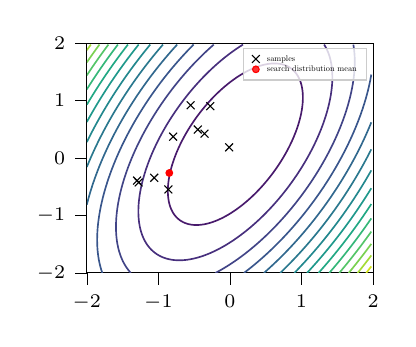
\begin{tikzpicture}

\definecolor{color0}{rgb}{0.282656,0.100196,0.42216}
\definecolor{color1}{rgb}{0.277134,0.185228,0.489898}
\definecolor{color2}{rgb}{0.253935,0.265254,0.529983}
\definecolor{color3}{rgb}{0.221989,0.339161,0.548752}
\definecolor{color4}{rgb}{0.190631,0.407061,0.556089}
\definecolor{color5}{rgb}{0.163625,0.471133,0.558148}
\definecolor{color6}{rgb}{0.139147,0.533812,0.555298}
\definecolor{color7}{rgb}{0.120565,0.596422,0.543611}
\definecolor{color8}{rgb}{0.134692,0.658636,0.517649}
\definecolor{color9}{rgb}{0.20803,0.718701,0.472873}
\definecolor{color10}{rgb}{0.327796,0.77398,0.40664}
\definecolor{color11}{rgb}{0.477504,0.821444,0.318195}
\definecolor{color12}{rgb}{0.647257,0.8584,0.209861}
\definecolor{color13}{rgb}{0.82494,0.88472,0.106217}
\definecolor{color14}{rgb}{0.12156862745098,0.466666666666667,0.705882352941177}

\begin{axis}[
legend cell align={left},
legend style={
  fill opacity=0.8,
  draw opacity=1,
  text opacity=1,
  draw=white!80!black,
  nodes={scale=0.3, transform shape}
},
tick align=outside,
tick pos=left,
ticklabel style = {font=\scriptsize},
height=4.5cm,
x grid style={white!69.0196078431373!black},
xmin=-2, xmax=2,
xtick style={color=black},
y grid style={white!69.0196078431373!black},
ymin=-2, ymax=2,
ytick style={color=black}
]
\addplot [draw=black, fill=black, mark=x, only marks,]
table{%
x  y
-1.0583486719713 -0.343634121064038
-0.275233370717191 0.902598501154073
-1.29808197620503 -0.391804407376918
-0.793672060934383 0.37194062733657
-1.27633407828662 -0.424654430436022
-0.549136953115668 0.917729542690637
-0.449568834306155 0.49617206320152
-0.355171005116645 0.424385765131947
-0.860513384577885 -0.546523389832645
-0.0111525131272885 0.186111314812185
};
\addlegendentry{$~$ samples}
\addplot [draw=red, fill=red, mark=*, only marks,
mark options={scale=0.6}]
table{
x  y
-0.847316845794121 -0.259789935392427
};
\addlegendentry{$~$ search distribution mean}
\path [draw=color0, semithick]
(axis cs:-0.575000000000005,-1.15156224853012)
--(axis cs:-0.579784331063212,-1.15)
--(axis cs:-0.600000000000005,-1.1430122164428)
--(axis cs:-0.625000000000005,-1.132138842302)
--(axis cs:-0.638549638581596,-1.125)
--(axis cs:-0.650000000000005,-1.11858068676859)
--(axis cs:-0.675000000000005,-1.1019707908525)
--(axis cs:-0.677573160208406,-1.1)
--(axis cs:-0.700000000000005,-1.08160891437882)
--(axis cs:-0.707052236225316,-1.075)
--(axis cs:-0.725000000000005,-1.05690097771229)
--(axis cs:-0.731083241794209,-1.05)
--(axis cs:-0.750000000000004,-1.02677347053858)
--(axis cs:-0.751300008753877,-1.025)
--(axis cs:-0.768304065280147,-1)
--(axis cs:-0.775000000000004,-0.989249737794899)
--(axis cs:-0.783089004132443,-0.975000000000004)
--(axis cs:-0.7960408579298,-0.950000000000004)
--(axis cs:-0.800000000000004,-0.941641773611196)
--(axis cs:-0.807255430188387,-0.925000000000004)
--(axis cs:-0.817128551154667,-0.900000000000004)
--(axis cs:-0.825000000000004,-0.877778706574327)
--(axis cs:-0.825913193608126,-0.875000000000004)
--(axis cs:-0.833374578688182,-0.850000000000004)
--(axis cs:-0.839983523715072,-0.825000000000004)
--(axis cs:-0.845788732574604,-0.800000000000004)
--(axis cs:-0.850000000000004,-0.779203384611521)
--(axis cs:-0.850796895896401,-0.775000000000004)
--(axis cs:-0.854931767700512,-0.750000000000004)
--(axis cs:-0.858425257584416,-0.725000000000005)
--(axis cs:-0.861309931807664,-0.700000000000005)
--(axis cs:-0.863616188582082,-0.675000000000005)
--(axis cs:-0.865372435536144,-0.650000000000005)
--(axis cs:-0.86660525002862,-0.625000000000005)
--(axis cs:-0.86733952421459,-0.600000000000005)
--(axis cs:-0.867598596529359,-0.575000000000005)
--(axis cs:-0.867404371051052,-0.550000000000005)
--(axis cs:-0.866777426025877,-0.525000000000005)
--(axis cs:-0.865737112686869,-0.500000000000005)
--(axis cs:-0.8643016453641,-0.475000000000005)
--(axis cs:-0.862488183768747,-0.450000000000006)
--(axis cs:-0.860312908232694,-0.425000000000006)
--(axis cs:-0.857791088597381,-0.400000000000006)
--(axis cs:-0.8549371473686,-0.375000000000006)
--(axis cs:-0.851764717686456,-0.350000000000006)
--(axis cs:-0.850000000000004,-0.33740014404947)
--(axis cs:-0.848224964045552,-0.325000000000006)
--(axis cs:-0.844320398509125,-0.300000000000006)
--(axis cs:-0.840127764885079,-0.275000000000006)
--(axis cs:-0.83565866206016,-0.250000000000006)
--(axis cs:-0.830924074471746,-0.225000000000006)
--(axis cs:-0.825934412263982,-0.200000000000006)
--(axis cs:-0.825000000000004,-0.195584958935086)
--(axis cs:-0.820551676940746,-0.175000000000006)
--(axis cs:-0.814897295651725,-0.150000000000007)
--(axis cs:-0.809013156052254,-0.125000000000007)
--(axis cs:-0.802908102823562,-0.100000000000007)
--(axis cs:-0.800000000000004,-0.0885711506293182)
--(axis cs:-0.796475483222582,-0.0750000000000068)
--(axis cs:-0.789737621969138,-0.0500000000000069)
--(axis cs:-0.782801832342293,-0.025000000000007)
--(axis cs:-0.775675597032023,-7.105427357601e-15)
--(axis cs:-0.775000000000004,0.00228453096550625)
--(axis cs:-0.768146266213347,0.0249999999999928)
--(axis cs:-0.760418068664097,0.0499999999999927)
--(axis cs:-0.752520301713795,0.0749999999999926)
--(axis cs:-0.750000000000004,0.0827495375406521)
--(axis cs:-0.744276711963535,0.0999999999999925)
--(axis cs:-0.73579334510844,0.124999999999992)
--(axis cs:-0.727160136040372,0.149999999999992)
--(axis cs:-0.725000000000005,0.156095174940785)
--(axis cs:-0.718165771812414,0.174999999999992)
--(axis cs:-0.708963417774858,0.199999999999992)
--(axis cs:-0.700000000000005,0.22399658418107)
--(axis cs:-0.699617624467883,0.224999999999992)
--(axis cs:-0.689849469479751,0.249999999999992)
--(axis cs:-0.679963286102105,0.274999999999992)
--(axis cs:-0.675000000000005,0.287330824774297)
--(axis cs:-0.669798075342292,0.299999999999992)
--(axis cs:-0.659363060831134,0.324999999999992)
--(axis cs:-0.650000000000005,0.347186075029143)
--(axis cs:-0.648788421075721,0.349999999999992)
--(axis cs:-0.637808700483621,0.374999999999992)
--(axis cs:-0.626741054228276,0.399999999999991)
--(axis cs:-0.625000000000005,0.403862107084494)
--(axis cs:-0.615279134770556,0.424999999999991)
--(axis cs:-0.603684254574478,0.449999999999991)
--(axis cs:-0.600000000000005,0.457827071766688)
--(axis cs:-0.591752668405044,0.474999999999991)
--(axis cs:-0.579635494303139,0.499999999999991)
--(axis cs:-0.575000000000005,0.509442839706575)
--(axis cs:-0.567206957755413,0.524999999999991)
--(axis cs:-0.55457282493635,0.549999999999991)
--(axis cs:-0.550000000000005,0.558941914502023)
--(axis cs:-0.541618986443886,0.574999999999991)
--(axis cs:-0.528473645665061,0.599999999999991)
--(axis cs:-0.525000000000005,0.60652709797819)
--(axis cs:-0.51496503983484,0.624999999999991)
--(axis cs:-0.501314678932729,0.649999999999991)
--(axis cs:-0.500000000000005,0.652376086313625)
--(axis cs:-0.487220678353259,0.67499999999999)
--(axis cs:-0.475000000000005,0.696554300991851)
--(axis cs:-0.473004687137105,0.69999999999999)
--(axis cs:-0.458360709570299,0.72499999999999)
--(axis cs:-0.450000000000006,0.739195856959489)
--(axis cs:-0.44349996737351,0.74999999999999)
--(axis cs:-0.428359158989013,0.77499999999999)
--(axis cs:-0.425000000000006,0.780495305584987)
--(axis cs:-0.412818688045394,0.79999999999999)
--(axis cs:-0.400000000000006,0.820453472337604)
--(axis cs:-0.397087427087551,0.82499999999999)
--(axis cs:-0.38093263784212,0.84999999999999)
--(axis cs:-0.375000000000006,0.859126907080497)
--(axis cs:-0.364451683685915,0.87499999999999)
--(axis cs:-0.350000000000006,0.896673204758622)
--(axis cs:-0.347730993945698,0.89999999999999)
--(axis cs:-0.330541898035909,0.92499999999999)
--(axis cs:-0.325000000000006,0.933018507929147)
--(axis cs:-0.312992934833016,0.94999999999999)
--(axis cs:-0.300000000000006,0.968315445146141)
--(axis cs:-0.295146119373767,0.97499999999999)
--(axis cs:-0.276904650703425,0.999999999999989)
--(axis cs:-0.275000000000006,1.0025918158842)
--(axis cs:-0.258141001385961,1.02499999999999)
--(axis cs:-0.250000000000006,1.03578614516322)
--(axis cs:-0.239010362362972,1.04999999999999)
--(axis cs:-0.225000000000006,1.06806324723325)
--(axis cs:-0.21948522442503,1.07499999999999)
--(axis cs:-0.200000000000006,1.09943183709738)
--(axis cs:-0.1995352584843,1.09999999999999)
--(axis cs:-0.178956864730454,1.12499999999999)
--(axis cs:-0.175000000000006,1.12979049576146)
--(axis cs:-0.157875482092401,1.14999999999999)
--(axis cs:-0.150000000000007,1.15926565588256)
--(axis cs:-0.136271208546154,1.17499999999999)
--(axis cs:-0.125000000000007,1.18787812527748)
--(axis cs:-0.114101249834875,1.19999999999999)
--(axis cs:-0.100000000000007,1.21563581816783)
--(axis cs:-0.0913180109303491,1.22499999999999)
--(axis cs:-0.0750000000000068,1.24254655226488)
--(axis cs:-0.0678684034039275,1.24999999999999)
--(axis cs:-0.0500000000000069,1.26861805023614)
--(axis cs:-0.043693029320062,1.27499999999999)
--(axis cs:-0.025000000000007,1.29385794114542)
--(axis cs:-0.0187252151844623,1.29999999999999)
--(axis cs:-7.105427357601e-15,1.31827376186669)
--(axis cs:0.00711013720995598,1.32499999999999)
--(axis cs:0.0249999999999928,1.3418729584724)
--(axis cs:0.033897924848734,1.34999999999999)
--(axis cs:0.0499999999999927,1.36466288759682)
--(axis cs:0.0617344955609987,1.37499999999999)
--(axis cs:0.0749999999999926,1.38665081777488)
--(axis cs:0.0907296459925555,1.39999999999999)
--(axis cs:0.0999999999999925,1.40784393075702)
--(axis cs:0.121009053039111,1.42499999999999)
--(axis cs:0.124999999999992,1.42824932280055)
--(axis cs:0.149999999999992,1.44782710299503)
--(axis cs:0.152894731171929,1.44999999999999)
--(axis cs:0.174999999999992,1.46654289902265)
--(axis cs:0.186771143995696,1.47499999999999)
--(axis cs:0.199999999999992,1.48447575923823)
--(axis cs:0.222614390208175,1.49999999999999)
--(axis cs:0.224999999999992,1.50163274261311)
--(axis cs:0.249999999999992,1.51786530692392)
--(axis cs:0.261549537489041,1.52499999999999)
--(axis cs:0.274999999999992,1.5332836103926)
--(axis cs:0.299999999999992,1.54788439589719)
--(axis cs:0.30386934256326,1.54999999999999)
--(axis cs:0.324999999999992,1.56151755233117)
--(axis cs:0.349999999999992,1.57436420412909)
--(axis cs:0.351343030985569,1.57499999999999)
--(axis cs:0.374999999999992,1.58616395896542)
--(axis cs:0.399999999999991,1.597124443371)
--(axis cs:0.407233091616283,1.59999999999999)
--(axis cs:0.424999999999991,1.60704067039398)
--(axis cs:0.449999999999991,1.61597236887245)
--(axis cs:0.474999999999991,1.6239275161039)
--(axis cs:0.47894688392069,1.62499999999999)
--(axis cs:0.499999999999991,1.63070168466398)
--(axis cs:0.524999999999991,1.63636306730734)
--(axis cs:0.549999999999991,1.6408659491561)
--(axis cs:0.574999999999991,1.6441327977821)
--(axis cs:0.599999999999991,1.64607900444105)
--(axis cs:0.624999999999991,1.64661205791032)
--(axis cs:0.649999999999991,1.64563059981389)
--(axis cs:0.67499999999999,1.6430233411144)
--(axis cs:0.69999999999999,1.63866781537071)
--(axis cs:0.72499999999999,1.63242893933153)
--(axis cs:0.747512234802722,1.62499999999999)
--(axis cs:0.74999999999999,1.62413070139774)
--(axis cs:0.77499999999999,1.61331972203992)
--(axis cs:0.79999999999999,1.60002700129761)
--(axis cs:0.800043452425371,1.59999999999999)
--(axis cs:0.82499999999999,1.58346188351306)
--(axis cs:0.835951103906925,1.57499999999999)
--(axis cs:0.84999999999999,1.5633720588216)
--(axis cs:0.864142467280869,1.54999999999999)
--(axis cs:0.87499999999999,1.53894751255572)
--(axis cs:0.887183021193705,1.52499999999999)
--(axis cs:0.89999999999999,1.50910943994749)
--(axis cs:0.906614429575996,1.49999999999999)
--(axis cs:0.923308379825457,1.47499999999999)
--(axis cs:0.92499999999999,1.47225536156837)
--(axis cs:0.937503213850076,1.44999999999999)
--(axis cs:0.94999999999999,1.42541887809394)
--(axis cs:0.950195643947795,1.42499999999999)
--(axis cs:0.960964406071543,1.39999999999999)
--(axis cs:0.970634894768787,1.37499999999999)
--(axis cs:0.974999999999989,1.3625072782617)
--(axis cs:0.97905492780253,1.34999999999999)
--(axis cs:0.986346574960197,1.32499999999999)
--(axis cs:0.992793522921193,1.29999999999999)
--(axis cs:0.998443968929374,1.27499999999999)
--(axis cs:0.999999999999989,1.26716044569449)
--(axis cs:1.00318914815726,1.24999999999999)
--(axis cs:1.00719100805281,1.22499999999999)
--(axis cs:1.01055683392105,1.19999999999999)
--(axis cs:1.01331888219609,1.17499999999999)
--(axis cs:1.0155072643939,1.14999999999999)
--(axis cs:1.01715012248212,1.12499999999999)
--(axis cs:1.01827378732061,1.09999999999999)
--(axis cs:1.01890292204936,1.07499999999999)
--(axis cs:1.01906065206601,1.04999999999999)
--(axis cs:1.01876868303385,1.02499999999999)
--(axis cs:1.01804740818683,0.999999999999989)
--(axis cs:1.01691600604721,0.974999999999989)
--(axis cs:1.01539252954061,0.94999999999999)
--(axis cs:1.01349398737911,0.92499999999999)
--(axis cs:1.01123641848406,0.89999999999999)
--(axis cs:1.00863496013327,0.87499999999999)
--(axis cs:1.00570391044133,0.84999999999999)
--(axis cs:1.00245678571544,0.82499999999999)
--(axis cs:0.999999999999989,0.807773238723372)
--(axis cs:0.998867006976523,0.79999999999999)
--(axis cs:0.994889578923002,0.77499999999999)
--(axis cs:0.990626337902504,0.74999999999999)
--(axis cs:0.986088781179362,0.72499999999999)
--(axis cs:0.981287797517115,0.69999999999999)
--(axis cs:0.976233706909471,0.67499999999999)
--(axis cs:0.974999999999989,0.669235527434164)
--(axis cs:0.970796697125404,0.649999999999991)
--(axis cs:0.965079573914532,0.624999999999991)
--(axis cs:0.959134531277376,0.599999999999991)
--(axis cs:0.952970335218026,0.574999999999991)
--(axis cs:0.94999999999999,0.563430889218547)
--(axis cs:0.946480525262916,0.549999999999991)
--(axis cs:0.939685156497164,0.524999999999991)
--(axis cs:0.932693502913215,0.499999999999991)
--(axis cs:0.925512978514458,0.474999999999991)
--(axis cs:0.92499999999999,0.473278269114002)
--(axis cs:0.917923937561052,0.449999999999991)
--(axis cs:0.910143035172253,0.424999999999991)
--(axis cs:0.902194032435443,0.399999999999991)
--(axis cs:0.89999999999999,0.39329859070499)
--(axis cs:0.893888399377859,0.374999999999992)
--(axis cs:0.885355371167881,0.349999999999992)
--(axis cs:0.876673868983822,0.324999999999992)
--(axis cs:0.87499999999999,0.320305282066764)
--(axis cs:0.86761525910812,0.299999999999992)
--(axis cs:0.858366175537962,0.274999999999992)
--(axis cs:0.84999999999999,0.252729964646229)
--(axis cs:0.848953738347289,0.249999999999992)
--(axis cs:0.839140447781893,0.224999999999992)
--(axis cs:0.829210358855668,0.199999999999992)
--(axis cs:0.82499999999999,0.189594147324003)
--(axis cs:0.818976470242225,0.174999999999992)
--(axis cs:0.808499131225988,0.149999999999992)
--(axis cs:0.79999999999999,0.129960847605851)
--(axis cs:0.797853429519912,0.124999999999992)
--(axis cs:0.786832995058202,0.0999999999999925)
--(axis cs:0.77572573032623,0.0749999999999926)
--(axis cs:0.77499999999999,0.0733974861851043)
--(axis cs:0.764190881847721,0.0499999999999927)
--(axis cs:0.752557978867978,0.0249999999999928)
--(axis cs:0.74999999999999,0.0195893770325147)
--(axis cs:0.740551098708226,-7.105427357601e-15)
--(axis cs:0.728397526225616,-0.025000000000007)
--(axis cs:0.72499999999999,-0.031892083369148)
--(axis cs:0.715891305068967,-0.0500000000000069)
--(axis cs:0.703222427223513,-0.0750000000000068)
--(axis cs:0.69999999999999,-0.0812760388799322)
--(axis cs:0.690188488320584,-0.100000000000007)
--(axis cs:0.677010085042015,-0.125000000000007)
--(axis cs:0.67499999999999,-0.128762499636892)
--(axis cs:0.663418938353691,-0.150000000000007)
--(axis cs:0.649999999999991,-0.174513657829444)
--(axis cs:0.649728139893546,-0.175000000000006)
--(axis cs:0.635558220931034,-0.200000000000006)
--(axis cs:0.624999999999991,-0.218554069768133)
--(axis cs:0.62125371472572,-0.225000000000006)
--(axis cs:0.606581149830409,-0.250000000000006)
--(axis cs:0.599999999999991,-0.261135062884442)
--(axis cs:0.591629296613889,-0.275000000000006)
--(axis cs:0.576461757691618,-0.300000000000006)
--(axis cs:0.574999999999991,-0.302383242868402)
--(axis cs:0.560827556259066,-0.325000000000006)
--(axis cs:0.549999999999991,-0.3422187246191)
--(axis cs:0.544998601997116,-0.350000000000006)
--(axis cs:0.52882029148226,-0.375000000000006)
--(axis cs:0.524999999999991,-0.380858348874797)
--(axis cs:0.51223888514279,-0.400000000000006)
--(axis cs:0.499999999999991,-0.418296375313372)
--(axis cs:0.495413399604953,-0.425000000000006)
--(axis cs:0.478204360865758,-0.450000000000006)
--(axis cs:0.474999999999991,-0.45462219061757)
--(axis cs:0.460547695775477,-0.475000000000005)
--(axis cs:0.449999999999991,-0.489823645329519)
--(axis cs:0.442588414230013,-0.500000000000005)
--(axis cs:0.424999999999991,-0.524070740363962)
--(axis cs:0.424304604441359,-0.525000000000005)
--(axis cs:0.405451817498191,-0.550000000000005)
--(axis cs:0.399999999999991,-0.557202499903312)
--(axis cs:0.386200422616391,-0.575000000000005)
--(axis cs:0.374999999999992,-0.589399618703327)
--(axis cs:0.366548939003484,-0.600000000000005)
--(axis cs:0.349999999999992,-0.620692269240568)
--(axis cs:0.346466642849775,-0.625000000000005)
--(axis cs:0.325881726465351,-0.650000000000005)
--(axis cs:0.324999999999992,-0.651064628386651)
--(axis cs:0.304664475793667,-0.675000000000005)
--(axis cs:0.299999999999992,-0.680473365267421)
--(axis cs:0.282917743435903,-0.700000000000005)
--(axis cs:0.274999999999992,-0.709023072623961)
--(axis cs:0.260598248257185,-0.725000000000005)
--(axis cs:0.249999999999992,-0.736721601444483)
--(axis cs:0.237657859781785,-0.750000000000004)
--(axis cs:0.224999999999992,-0.76357670733699)
--(axis cs:0.214042899453584,-0.775000000000004)
--(axis cs:0.199999999999992,-0.789596051973344)
--(axis cs:0.189693317494214,-0.800000000000004)
--(axis cs:0.174999999999992,-0.814787204507165)
--(axis cs:0.164541718728919,-0.825000000000004)
--(axis cs:0.149999999999992,-0.839157642966126)
--(axis cs:0.138512204029826,-0.850000000000004)
--(axis cs:0.124999999999992,-0.86271475561919)
--(axis cs:0.111518985335867,-0.875000000000004)
--(axis cs:0.0999999999999925,-0.885465842319292)
--(axis cs:0.0834647208846994,-0.900000000000004)
--(axis cs:0.0749999999999926,-0.907418115821998)
--(axis cs:0.0542385024171835,-0.925000000000004)
--(axis cs:0.0499999999999927,-0.928578703080634)
--(axis cs:0.0249999999999928,-0.948931600705651)
--(axis cs:0.0236327392308407,-0.950000000000004)
--(axis cs:-7.105427357601e-15,-0.968411202371224)
--(axis cs:-0.00879482540931608,-0.975000000000004)
--(axis cs:-0.025000000000007,-0.987103820491066)
--(axis cs:-0.0429834578864496,-1)
--(axis cs:-0.0500000000000069,-1.00501654552679)
--(axis cs:-0.0750000000000068,-1.02209306441058)
--(axis cs:-0.0794795939255493,-1.025)
--(axis cs:-0.100000000000007,-1.03827563824622)
--(axis cs:-0.119009538100499,-1.05)
--(axis cs:-0.125000000000007,-1.0536834493061)
--(axis cs:-0.150000000000007,-1.06817291225977)
--(axis cs:-0.1625031061602,-1.075)
--(axis cs:-0.175000000000006,-1.0818025974741)
--(axis cs:-0.200000000000006,-1.09454063393289)
--(axis cs:-0.211543270725672,-1.1)
--(axis cs:-0.225000000000006,-1.10634432825863)
--(axis cs:-0.250000000000006,-1.1171997224403)
--(axis cs:-0.269628648647289,-1.125)
--(axis cs:-0.275000000000006,-1.12712771240956)
--(axis cs:-0.300000000000006,-1.13595877371075)
--(axis cs:-0.325000000000006,-1.14381309384101)
--(axis cs:-0.347739527654627,-1.15)
--(axis cs:-0.350000000000006,-1.150612981859)
--(axis cs:-0.375000000000006,-1.15617973739594)
--(axis cs:-0.400000000000006,-1.16058883382305)
--(axis cs:-0.425000000000006,-1.1637631336932)
--(axis cs:-0.450000000000006,-1.16561849076503)
--(axis cs:-0.475000000000005,-1.16606293546696)
--(axis cs:-0.500000000000005,-1.16499574406333)
--(axis cs:-0.525000000000005,-1.16230637167801)
--(axis cs:-0.550000000000005,-1.15787322536454)
--(axis cs:-0.575000000000005,-1.15156224853012);

\path [draw=color1, semithick]
(axis cs:1.31542009442798,1.97499999999999)
--(axis cs:1.32499999999999,1.95639267718934)
--(axis cs:1.32810030506846,1.94999999999999)
--(axis cs:1.33951907940095,1.92499999999999)
--(axis cs:1.34999999999999,1.9002961448008)
--(axis cs:1.35011885776589,1.89999999999999)
--(axis cs:1.35957043647575,1.87499999999999)
--(axis cs:1.36832011322874,1.84999999999999)
--(axis cs:1.37499999999999,1.82937972652429)
--(axis cs:1.37634812988178,1.82499999999999)
--(axis cs:1.38352106971695,1.79999999999999)
--(axis cs:1.39010689397533,1.77499999999999)
--(axis cs:1.39612914950941,1.74999999999999)
--(axis cs:1.39999999999999,1.7324132719063)
--(axis cs:1.40155721089687,1.72499999999999)
--(axis cs:1.40635772413055,1.69999999999999)
--(axis cs:1.4106781907869,1.67499999999999)
--(axis cs:1.41453630771798,1.64999999999999)
--(axis cs:1.41794891247907,1.62499999999999)
--(axis cs:1.42093203485869,1.59999999999999)
--(axis cs:1.42350094474433,1.57499999999999)
--(axis cs:1.42499999999999,1.55778684840957)
--(axis cs:1.42565056418239,1.54999999999999)
--(axis cs:1.42738260226577,1.52499999999999)
--(axis cs:1.42875392169716,1.49999999999999)
--(axis cs:1.42977642020876,1.47499999999999)
--(axis cs:1.43046147798581,1.44999999999999)
--(axis cs:1.43081998550529,1.42499999999999)
--(axis cs:1.4308623695967,1.39999999999999)
--(axis cs:1.43059861785619,1.37499999999999)
--(axis cs:1.43003830153412,1.34999999999999)
--(axis cs:1.42919059700611,1.32499999999999)
--(axis cs:1.42806430592904,1.29999999999999)
--(axis cs:1.42666787417491,1.27499999999999)
--(axis cs:1.42500940962807,1.24999999999999)
--(axis cs:1.42499999999999,1.24987822419071)
--(axis cs:1.4230468518292,1.22499999999999)
--(axis cs:1.42083189054114,1.19999999999999)
--(axis cs:1.41837231085751,1.17499999999999)
--(axis cs:1.4156753515581,1.14999999999999)
--(axis cs:1.41274796859792,1.12499999999999)
--(axis cs:1.40959684878633,1.09999999999999)
--(axis cs:1.40622842267983,1.07499999999999)
--(axis cs:1.40264887674079,1.04999999999999)
--(axis cs:1.39999999999999,1.03255247451693)
--(axis cs:1.39883597175446,1.02499999999999)
--(axis cs:1.3947541463036,0.999999999999989)
--(axis cs:1.3904755316474,0.97499999999999)
--(axis cs:1.38600565547987,0.94999999999999)
--(axis cs:1.38134984038914,0.92499999999999)
--(axis cs:1.37651321328322,0.89999999999999)
--(axis cs:1.37499999999999,0.892500916902506)
--(axis cs:1.37141663019958,0.87499999999999)
--(axis cs:1.36611039238015,0.84999999999999)
--(axis cs:1.36063595334116,0.82499999999999)
--(axis cs:1.35499789101292,0.79999999999999)
--(axis cs:1.34999999999999,0.778474158608702)
--(axis cs:1.34918166207204,0.77499999999999)
--(axis cs:1.34308974418138,0.74999999999999)
--(axis cs:1.33684599030513,0.72499999999999)
--(axis cs:1.33045448027279,0.69999999999999)
--(axis cs:1.32499999999999,0.6791655071137)
--(axis cs:1.32389384909898,0.674999999999991)
--(axis cs:1.3170638747433,0.649999999999991)
--(axis cs:1.31009716403529,0.624999999999991)
--(axis cs:1.3029973448236,0.599999999999991)
--(axis cs:1.29999999999999,0.589688301399073)
--(axis cs:1.29567012031315,0.574999999999991)
--(axis cs:1.28814686584148,0.549999999999991)
--(axis cs:1.28050080684424,0.524999999999991)
--(axis cs:1.27499999999999,0.507336601956377)
--(axis cs:1.27268302184192,0.499999999999991)
--(axis cs:1.26462150858973,0.474999999999991)
--(axis cs:1.25644709716414,0.449999999999991)
--(axis cs:1.24999999999999,0.430582179331819)
--(axis cs:1.24812059829766,0.424999999999991)
--(axis cs:1.23953874731177,0.399999999999991)
--(axis cs:1.23085351766247,0.374999999999992)
--(axis cs:1.22499999999999,0.358392514491612)
--(axis cs:1.22200059796923,0.349999999999992)
--(axis cs:1.21291597415832,0.324999999999992)
--(axis cs:1.2037371148405,0.299999999999992)
--(axis cs:1.19999999999999,0.289974333162254)
--(axis cs:1.19434050352983,0.274999999999992)
--(axis cs:1.18477032327374,0.249999999999992)
--(axis cs:1.17511468451611,0.224999999999992)
--(axis cs:1.17499999999999,0.22470810588592)
--(axis cs:1.16515753698746,0.199999999999992)
--(axis cs:1.15511867556269,0.174999999999992)
--(axis cs:1.14999999999999,0.162404213773604)
--(axis cs:1.14488887188667,0.149999999999992)
--(axis cs:1.13446866452495,0.124999999999992)
--(axis cs:1.12499999999999,0.102455487981698)
--(axis cs:1.12395424119954,0.0999999999999925)
--(axis cs:1.11315468214034,0.0749999999999926)
--(axis cs:1.10229060123264,0.0499999999999927)
--(axis cs:1.09999999999999,0.0447952137321759)
--(axis cs:1.09116655548993,0.0249999999999928)
--(axis cs:1.07993153717919,-7.105427357601e-15)
--(axis cs:1.07499999999999,-0.0108647432648761)
--(axis cs:1.06849390277123,-0.025000000000007)
--(axis cs:1.05689021371451,-0.0500000000000069)
--(axis cs:1.04999999999999,-0.0647273705303289)
--(axis cs:1.04512612790921,-0.0750000000000068)
--(axis cs:1.03315616353351,-0.100000000000007)
--(axis cs:1.02499999999999,-0.116923547969012)
--(axis cs:1.0210524149996,-0.125000000000007)
--(axis cs:1.00871870410958,-0.150000000000007)
--(axis cs:0.999999999999989,-0.167571749217071)
--(axis cs:0.996261722578345,-0.175000000000006)
--(axis cs:0.983566932134499,-0.200000000000006)
--(axis cs:0.974999999999989,-0.216779477619462)
--(axis cs:0.970742777710913,-0.225000000000006)
--(axis cs:0.957689717785011,-0.250000000000006)
--(axis cs:0.949999999999989,-0.264644507269515)
--(axis cs:0.944484069894695,-0.275000000000006)
--(axis cs:0.931075698809844,-0.300000000000006)
--(axis cs:0.92499999999999,-0.311255959301409)
--(axis cs:0.917473844767681,-0.325000000000006)
--(axis cs:0.903713274430525,-0.350000000000006)
--(axis cs:0.89999999999999,-0.356695238398328)
--(axis cs:0.889700097616119,-0.375000000000006)
--(axis cs:0.875590599049117,-0.400000000000006)
--(axis cs:0.87499999999999,-0.401036850247909)
--(axis cs:0.86115056667365,-0.425000000000006)
--(axis cs:0.84999999999999,-0.444244128071074)
--(axis cs:0.846615345901289,-0.450000000000006)
--(axis cs:0.831812726204058,-0.475000000000005)
--(axis cs:0.82499999999999,-0.486452722369652)
--(axis cs:0.816820939355015,-0.500000000000005)
--(axis cs:0.801673779359448,-0.525000000000005)
--(axis cs:0.79999999999999,-0.527741864443768)
--(axis cs:0.78620837912557,-0.550000000000005)
--(axis cs:0.77499999999999,-0.568044854632416)
--(axis cs:0.770614007203846,-0.575000000000005)
--(axis cs:0.754764109970214,-0.600000000000005)
--(axis cs:0.74999999999999,-0.607476594141515)
--(axis cs:0.738662812131983,-0.625000000000005)
--(axis cs:0.72499999999999,-0.646067546751275)
--(axis cs:0.722409994559096,-0.650000000000005)
--(axis cs:0.705847295813209,-0.675000000000005)
--(axis cs:0.69999999999999,-0.683791866294034)
--(axis cs:0.689051462308331,-0.700000000000005)
--(axis cs:0.67499999999999,-0.720753037722802)
--(axis cs:0.672078715130083,-0.725000000000005)
--(axis cs:0.654793801862975,-0.750000000000004)
--(axis cs:0.649999999999991,-0.756905938423435)
--(axis cs:0.637238876649345,-0.775000000000004)
--(axis cs:0.624999999999991,-0.792313847277157)
--(axis cs:0.619478415787233,-0.800000000000004)
--(axis cs:0.601462701641466,-0.825000000000004)
--(axis cs:0.599999999999991,-0.827018880392155)
--(axis cs:0.583077495364553,-0.850000000000004)
--(axis cs:0.574999999999991,-0.860944825312103)
--(axis cs:0.564454462761437,-0.875000000000004)
--(axis cs:0.549999999999991,-0.894221941428676)
--(axis cs:0.545581535159606,-0.900000000000004)
--(axis cs:0.526406268332886,-0.925000000000004)
--(axis cs:0.524999999999991,-0.926824950933203)
--(axis cs:0.506837844609846,-0.950000000000004)
--(axis cs:0.499999999999991,-0.958706027513455)
--(axis cs:0.486980877212822,-0.975000000000004)
--(axis cs:0.474999999999991,-0.989961787770765)
--(axis cs:0.466820113424564,-1)
--(axis cs:0.449999999999991,-1.02059632348148)
--(axis cs:0.446339206213054,-1.025)
--(axis cs:0.425505524857996,-1.05)
--(axis cs:0.424999999999991,-1.05060412584982)
--(axis cs:0.404217267729844,-1.075)
--(axis cs:0.399999999999991,-1.07993986897797)
--(axis cs:0.382559366234335,-1.1)
--(axis cs:0.374999999999992,-1.10867619671701)
--(axis cs:0.360511048734672,-1.125)
--(axis cs:0.349999999999992,-1.13681693721803)
--(axis cs:0.338049957576135,-1.15)
--(axis cs:0.324999999999992,-1.16436588610352)
--(axis cs:0.315151994764833,-1.175)
--(axis cs:0.299999999999992,-1.19132680681212)
--(axis cs:0.291791149270081,-1.2)
--(axis cs:0.274999999999992,-1.21770343093906)
--(axis cs:0.267939303345803,-1.225)
--(axis cs:0.249999999999992,-1.24349945857218)
--(axis cs:0.243566014835676,-1.25)
--(axis cs:0.224999999999992,-1.26871855862383)
--(axis cs:0.218638271914347,-1.275)
--(axis cs:0.199999999999992,-1.29336436915847)
--(axis cs:0.193120216105188,-1.3)
--(axis cs:0.174999999999992,-1.31744049771624)
--(axis cs:0.166972828681892,-1.325)
--(axis cs:0.149999999999992,-1.34095052163238)
--(axis cs:0.140153574679393,-1.35)
--(axis cs:0.124999999999992,-1.36389798835273)
--(axis cs:0.112615997674837,-1.375)
--(axis cs:0.0999999999999925,-1.38628641574521)
--(axis cs:0.0843092572084932,-1.4)
--(axis cs:0.0749999999999926,-1.4081192924075)
--(axis cs:0.0551775991430002,-1.425)
--(axis cs:0.0499999999999927,-1.42940007797077)
--(axis cs:0.0251597473375424,-1.45)
--(axis cs:0.0249999999999928,-1.45013220339974)
--(axis cs:-7.105427357601e-15,-1.47024760374458)
--(axis cs:-0.00606339063585133,-1.475)
--(axis cs:-0.025000000000007,-1.48981115015674)
--(axis cs:-0.0383812721360449,-1.5)
--(axis cs:-0.0500000000000069,-1.50882831278571)
--(axis cs:-0.0718784547988801,-1.525)
--(axis cs:-0.0750000000000068,-1.52730251031841)
--(axis cs:-0.100000000000007,-1.54516391118527)
--(axis cs:-0.106985236651084,-1.55)
--(axis cs:-0.125000000000007,-1.56244585907409)
--(axis cs:-0.143737264250273,-1.575)
--(axis cs:-0.150000000000007,-1.57918726079026)
--(axis cs:-0.175000000000006,-1.59532002760188)
--(axis cs:-0.182524384328757,-1.6)
--(axis cs:-0.200000000000006,-1.6108462505212)
--(axis cs:-0.223605315436197,-1.625)
--(axis cs:-0.225000000000006,-1.6258344772129)
--(axis cs:-0.250000000000006,-1.64013607540115)
--(axis cs:-0.267923857596524,-1.65)
--(axis cs:-0.275000000000006,-1.6538858062803)
--(axis cs:-0.300000000000006,-1.66697512494646)
--(axis cs:-0.316052453474424,-1.675)
--(axis cs:-0.325000000000006,-1.67946330369264)
--(axis cs:-0.350000000000006,-1.69127799682553)
--(axis cs:-0.369454132124636,-1.7)
--(axis cs:-0.375000000000006,-1.70248095309688)
--(axis cs:-0.400000000000006,-1.71295527404601)
--(axis cs:-0.425000000000006,-1.72281334030539)
--(axis cs:-0.430997047572207,-1.725)
--(axis cs:-0.450000000000006,-1.73191328624404)
--(axis cs:-0.475000000000005,-1.74031372245323)
--(axis cs:-0.500000000000005,-1.7480210054714)
--(axis cs:-0.507159320841013,-1.75)
--(axis cs:-0.525000000000005,-1.75492014232942)
--(axis cs:-0.550000000000005,-1.7610394667072)
--(axis cs:-0.575000000000005,-1.7663783047418)
--(axis cs:-0.600000000000005,-1.77090109797693)
--(axis cs:-0.625000000000005,-1.77457009462009)
--(axis cs:-0.628924042441808,-1.775)
--(axis cs:-0.650000000000005,-1.77730335288206)
--(axis cs:-0.675000000000005,-1.77910789813018)
--(axis cs:-0.700000000000005,-1.77994742171098)
--(axis cs:-0.725000000000005,-1.77977523470198)
--(axis cs:-0.750000000000004,-1.77854158699016)
--(axis cs:-0.775000000000004,-1.7761934122048)
--(axis cs:-0.783571874620236,-1.775)
--(axis cs:-0.800000000000004,-1.77262743079657)
--(axis cs:-0.825000000000004,-1.7677785882596)
--(axis cs:-0.850000000000004,-1.76160274751762)
--(axis cs:-0.875000000000004,-1.75402732647511)
--(axis cs:-0.886235271397571,-1.75)
--(axis cs:-0.900000000000004,-1.74486376630114)
--(axis cs:-0.925000000000004,-1.73400914283437)
--(axis cs:-0.943039813345534,-1.725)
--(axis cs:-0.950000000000004,-1.72137251637879)
--(axis cs:-0.975000000000004,-1.70667258625204)
--(axis cs:-0.985129854687892,-1.7)
--(axis cs:-1,-1.68974882258988)
--(axis cs:-1.01924153916888,-1.675)
--(axis cs:-1.025,-1.67037049720664)
--(axis cs:-1.04802154534035,-1.65)
--(axis cs:-1.05,-1.64815947827703)
--(axis cs:-1.07280972363559,-1.625)
--(axis cs:-1.075,-1.62265576004519)
--(axis cs:-1.09453168484431,-1.6)
--(axis cs:-1.1,-1.5932940352752)
--(axis cs:-1.11384740172386,-1.575)
--(axis cs:-1.125,-1.55937173507363)
--(axis cs:-1.13124012296152,-1.55)
--(axis cs:-1.14693319424459,-1.525)
--(axis cs:-1.15,-1.51982512136359)
--(axis cs:-1.16102456362694,-1.5)
--(axis cs:-1.17401311373573,-1.475)
--(axis cs:-1.175,-1.47298766227864)
--(axis cs:-1.18562925002636,-1.45)
--(axis cs:-1.19638410191779,-1.425)
--(axis cs:-1.2,-1.41602571300398)
--(axis cs:-1.2061131563839,-1.4)
--(axis cs:-1.21499475030173,-1.375)
--(axis cs:-1.22320036439507,-1.35)
--(axis cs:-1.225,-1.34411253938841)
--(axis cs:-1.23055489674052,-1.325)
--(axis cs:-1.23725394213249,-1.3)
--(axis cs:-1.24338585988285,-1.275)
--(axis cs:-1.24897311593053,-1.25)
--(axis cs:-1.25,-1.24498316997548)
--(axis cs:-1.25390585364117,-1.225)
--(axis cs:-1.25832188736636,-1.2)
--(axis cs:-1.26227282185831,-1.175)
--(axis cs:-1.26577560923318,-1.15)
--(axis cs:-1.2688463876598,-1.125)
--(axis cs:-1.27150052963181,-1.1)
--(axis cs:-1.27375268684469,-1.075)
--(axis cs:-1.275,-1.05833694927153)
--(axis cs:-1.27559895178392,-1.05)
--(axis cs:-1.27704592126866,-1.025)
--(axis cs:-1.27814213593267,-1)
--(axis cs:-1.27889904778781,-0.975000000000004)
--(axis cs:-1.27932761567476,-0.950000000000004)
--(axis cs:-1.27943833152775,-0.925000000000004)
--(axis cs:-1.27924124497849,-0.900000000000004)
--(axis cs:-1.27874598642039,-0.875000000000004)
--(axis cs:-1.27796178864458,-0.850000000000004)
--(axis cs:-1.27689750714957,-0.825000000000004)
--(axis cs:-1.27556163921871,-0.800000000000004)
--(axis cs:-1.275,-0.791277761777038)
--(axis cs:-1.27393486691729,-0.775000000000004)
--(axis cs:-1.2720316392157,-0.750000000000004)
--(axis cs:-1.26987487904862,-0.725000000000005)
--(axis cs:-1.26747216902252,-0.700000000000005)
--(axis cs:-1.2648307923561,-0.675000000000005)
--(axis cs:-1.261957747512,-0.650000000000005)
--(axis cs:-1.25885976197862,-0.625000000000005)
--(axis cs:-1.25554330525929,-0.600000000000005)
--(axis cs:-1.25201460112128,-0.575000000000005)
--(axis cs:-1.25,-0.561573974519837)
--(axis cs:-1.24823690846548,-0.550000000000005)
--(axis cs:-1.24420504669659,-0.525000000000005)
--(axis cs:-1.23997532009704,-0.500000000000005)
--(axis cs:-1.23555329022627,-0.475000000000005)
--(axis cs:-1.230944312147,-0.450000000000006)
--(axis cs:-1.22615354392092,-0.425000000000006)
--(axis cs:-1.225,-0.419235354016026)
--(axis cs:-1.22109424818985,-0.400000000000006)
--(axis cs:-1.21583304043451,-0.375000000000006)
--(axis cs:-1.21040269833259,-0.350000000000006)
--(axis cs:-1.2048078281419,-0.325000000000006)
--(axis cs:-1.2,-0.304145564795057)
--(axis cs:-1.19903039551659,-0.300000000000006)
--(axis cs:-1.19298085833302,-0.275000000000006)
--(axis cs:-1.18677862234572,-0.250000000000006)
--(axis cs:-1.18042779314687,-0.225000000000006)
--(axis cs:-1.175,-0.204140019598012)
--(axis cs:-1.17390732311883,-0.200000000000006)
--(axis cs:-1.1671172355811,-0.175000000000006)
--(axis cs:-1.16018961382603,-0.150000000000007)
--(axis cs:-1.1531281091355,-0.125000000000007)
--(axis cs:-1.15,-0.114180325304284)
--(axis cs:-1.14584227794238,-0.100000000000007)
--(axis cs:-1.13835656135815,-0.0750000000000068)
--(axis cs:-1.13074730242813,-0.0500000000000069)
--(axis cs:-1.125,-0.031453227608734)
--(axis cs:-1.12297207767261,-0.025000000000007)
--(axis cs:-1.11494659107069,-7.105427357601e-15)
--(axis cs:-1.10680750386971,0.0249999999999928)
--(axis cs:-1.1,0.0455978698404325)
--(axis cs:-1.09852468647916,0.0499999999999927)
--(axis cs:-1.08997738977362,0.0749999999999926)
--(axis cs:-1.08132604619358,0.0999999999999925)
--(axis cs:-1.075,0.118025145988194)
--(axis cs:-1.07251788472964,0.124999999999992)
--(axis cs:-1.0634663807603,0.149999999999992)
--(axis cs:-1.05432000614334,0.174999999999992)
--(axis cs:-1.05,0.186635852892386)
--(axis cs:-1.04496918653099,0.199999999999992)
--(axis cs:-1.03543072869692,0.224999999999992)
--(axis cs:-1.02580620918146,0.249999999999992)
--(axis cs:-1.025,0.252059664166908)
--(axis cs:-1.01589584469495,0.274999999999992)
--(axis cs:-1.00588734440351,0.299999999999992)
--(axis cs:-1,0.314539859570785)
--(axis cs:-0.995705469849445,0.324999999999992)
--(axis cs:-0.98531485559286,0.349999999999992)
--(axis cs:-0.975000000000004,0.374645422802942)
--(axis cs:-0.974849517065108,0.374999999999992)
--(axis cs:-0.964078773087735,0.399999999999991)
--(axis cs:-0.953242963902549,0.424999999999991)
--(axis cs:-0.950000000000004,0.432393147714884)
--(axis cs:-0.942168923435234,0.449999999999991)
--(axis cs:-0.930961403732367,0.474999999999991)
--(axis cs:-0.925000000000004,0.488175731922192)
--(axis cs:-0.91957492415742,0.499999999999991)
--(axis cs:-0.907997950801166,0.524999999999991)
--(axis cs:-0.900000000000004,0.542148165197965)
--(axis cs:-0.896286178355288,0.549999999999991)
--(axis cs:-0.884342136917009,0.574999999999991)
--(axis cs:-0.875000000000004,0.594442740280037)
--(axis cs:-0.872291869144702,0.599999999999991)
--(axis cs:-0.859983278513552,0.624999999999991)
--(axis cs:-0.850000000000004,0.645179165207994)
--(axis cs:-0.847580953918172,0.649999999999991)
--(axis cs:-0.834910471082465,0.67499999999999)
--(axis cs:-0.825000000000004,0.694466025002724)
--(axis cs:-0.822142158426063,0.69999999999999)
--(axis cs:-0.809112583432252,0.72499999999999)
--(axis cs:-0.800000000000004,0.742402044246651)
--(axis cs:-0.7959639706706,0.74999999999999)
--(axis cs:-0.782578251767108,0.77499999999999)
--(axis cs:-0.775000000000004,0.789077181502158)
--(axis cs:-0.769034634605692,0.79999999999999)
--(axis cs:-0.755295873579206,0.82499999999999)
--(axis cs:-0.750000000000004,0.834573581130928)
--(axis cs:-0.741342143635356,0.84999999999999)
--(axis cs:-0.727253601347516,0.87499999999999)
--(axis cs:-0.725000000000005,0.878966403730369)
--(axis cs:-0.71287423390318,0.89999999999999)
--(axis cs:-0.700000000000005,0.922274687807421)
--(axis cs:-0.698401418797464,0.92499999999999)
--(axis cs:-0.683618377364947,0.94999999999999)
--(axis cs:-0.675000000000005,0.964523533027441)
--(axis cs:-0.668690259154383,0.974999999999989)
--(axis cs:-0.653561774636205,0.999999999999989)
--(axis cs:-0.650000000000005,1.00584849822013)
--(axis cs:-0.638161313911763,1.02499999999999)
--(axis cs:-0.625000000000005,1.04623892141416)
--(axis cs:-0.622633775741,1.04999999999999)
--(axis cs:-0.606801024817042,1.07499999999999)
--(axis cs:-0.600000000000005,1.08569772309581)
--(axis cs:-0.590767878357351,1.09999999999999)
--(axis cs:-0.575000000000005,1.1243688221177)
--(axis cs:-0.574585231191463,1.12499999999999)
--(axis cs:-0.558038029099317,1.14999999999999)
--(axis cs:-0.550000000000005,1.16211257238834)
--(axis cs:-0.541313732234184,1.17499999999999)
--(axis cs:-0.525000000000005,1.19914719380158)
--(axis cs:-0.524414674443957,1.19999999999999)
--(axis cs:-0.507143478009714,1.22499999999999)
--(axis cs:-0.500000000000005,1.23531287853437)
--(axis cs:-0.489663658862813,1.24999999999999)
--(axis cs:-0.475000000000005,1.27078807354392)
--(axis cs:-0.47198060013813,1.27499999999999)
--(axis cs:-0.453976682308629,1.29999999999999)
--(axis cs:-0.450000000000006,1.30550010411875)
--(axis cs:-0.43567034709888,1.32499999999999)
--(axis cs:-0.425000000000006,1.33948765304441)
--(axis cs:-0.417128635267049,1.34999999999999)
--(axis cs:-0.400000000000006,1.37282430031533)
--(axis cs:-0.398339593458545,1.37499999999999)
--(axis cs:-0.379173008165973,1.39999999999999)
--(axis cs:-0.375000000000006,1.40542610047697)
--(axis cs:-0.359690042519944,1.42499999999999)
--(axis cs:-0.350000000000006,1.43736158043912)
--(axis cs:-0.339921272520468,1.44999999999999)
--(axis cs:-0.325000000000006,1.46866981311294)
--(axis cs:-0.319851578402749,1.47499999999999)
--(axis cs:-0.300000000000006,1.49935491399479)
--(axis cs:-0.299464754759786,1.49999999999999)
--(axis cs:-0.278634826943619,1.52499999999999)
--(axis cs:-0.275000000000006,1.52935187499925)
--(axis cs:-0.25744239398777,1.54999999999999)
--(axis cs:-0.250000000000006,1.55873365498436)
--(axis cs:-0.235883540768802,1.57499999999999)
--(axis cs:-0.225000000000006,1.58751423938762)
--(axis cs:-0.213937659653301,1.59999999999999)
--(axis cs:-0.200000000000006,1.61569747784903)
--(axis cs:-0.191582568175192,1.62499999999999)
--(axis cs:-0.175000000000006,1.64328718721134)
--(axis cs:-0.168794355670059,1.64999999999999)
--(axis cs:-0.150000000000007,1.67028715186862)
--(axis cs:-0.14554721163076,1.67499999999999)
--(axis cs:-0.125000000000007,1.69670112411031)
--(axis cs:-0.12181323319121,1.69999999999999)
--(axis cs:-0.100000000000007,1.722532824461)
--(axis cs:-0.0975622087160926,1.72499999999999)
--(axis cs:-0.0750000000000068,1.74778594201578)
--(axis cs:-0.0727613739635253,1.74999999999999)
--(axis cs:-0.0500000000000069,1.77246413477148)
--(axis cs:-0.0473751366778678,1.77499999999999)
--(axis cs:-0.025000000000007,1.79657102995365)
--(axis cs:-0.0213647647388596,1.79999999999999)
--(axis cs:-7.105427357601e-15,1.82011022433943)
--(axis cs:0.00531196788597558,1.82499999999999)
--(axis cs:0.0249999999999928,1.8430852845764)
--(axis cs:0.0327011842006435,1.84999999999999)
--(axis cs:0.0499999999999927,1.86549974749739)
--(axis cs:0.0608533643542607,1.87499999999999)
--(axis cs:0.0749999999999926,1.88735712043137)
--(axis cs:0.0898238725993691,1.89999999999999)
--(axis cs:0.0999999999999925,1.90866088151048)
--(axis cs:0.119673562623108,1.92499999999999)
--(axis cs:0.124999999999992,1.92941447997317)
--(axis cs:0.149999999999992,1.94961554007739)
--(axis cs:0.150489822798854,1.94999999999999)
--(axis cs:0.174999999999992,1.96919754235594)
--(axis cs:0.182610015495741,1.97499999999999);

\path [draw=color2, semithick]
(axis cs:-1.38453370092853,-2)
--(axis cs:-1.4,-1.97862826859581)
--(axis cs:-1.40248071213775,-1.975)
--(axis cs:-1.41883532864573,-1.95)
--(axis cs:-1.425,-1.94010263544659)
--(axis cs:-1.43392165438189,-1.925)
--(axis cs:-1.44794121442338,-1.9)
--(axis cs:-1.45,-1.89615293985183)
--(axis cs:-1.46077246042142,-1.875)
--(axis cs:-1.47280350518077,-1.85)
--(axis cs:-1.475,-1.84520594909254)
--(axis cs:-1.48383597109703,-1.825)
--(axis cs:-1.49415509314831,-1.8)
--(axis cs:-1.5,-1.78501489651421)
--(axis cs:-1.50373811312536,-1.775)
--(axis cs:-1.51256929126476,-1.75)
--(axis cs:-1.52085215779978,-1.725)
--(axis cs:-1.525,-1.71169889938896)
--(axis cs:-1.52850102426308,-1.7)
--(axis cs:-1.53553673816849,-1.675)
--(axis cs:-1.54209748420704,-1.65)
--(axis cs:-1.54819880964703,-1.625)
--(axis cs:-1.55,-1.61709844761631)
--(axis cs:-1.55375127096669,-1.6)
--(axis cs:-1.55883889039,-1.575)
--(axis cs:-1.56352374278917,-1.55)
--(axis cs:-1.56781812936359,-1.525)
--(axis cs:-1.57173385542791,-1.5)
--(axis cs:-1.575,-1.47700704096929)
--(axis cs:-1.57527518109176,-1.475)
--(axis cs:-1.57838798066818,-1.45)
--(axis cs:-1.58116481685876,-1.425)
--(axis cs:-1.58361521578425,-1.4)
--(axis cs:-1.58574834679115,-1.375)
--(axis cs:-1.58757303899931,-1.35)
--(axis cs:-1.58909779693687,-1.325)
--(axis cs:-1.59033081532101,-1.3)
--(axis cs:-1.59127999303817,-1.275)
--(axis cs:-1.59195294637409,-1.25)
--(axis cs:-1.59235702154017,-1.225)
--(axis cs:-1.59249930653931,-1.2)
--(axis cs:-1.59238664241166,-1.175)
--(axis cs:-1.59202563389772,-1.15)
--(axis cs:-1.59142265955366,-1.125)
--(axis cs:-1.59058388135141,-1.1)
--(axis cs:-1.58951525379399,-1.075)
--(axis cs:-1.58822253257427,-1.05)
--(axis cs:-1.58671128280363,-1.025)
--(axis cs:-1.58498688683539,-1)
--(axis cs:-1.58305455170589,-0.975000000000004)
--(axis cs:-1.58091931621499,-0.950000000000004)
--(axis cs:-1.57858605766616,-0.925000000000004)
--(axis cs:-1.57605949828513,-0.900000000000004)
--(axis cs:-1.575,-0.890292118436145)
--(axis cs:-1.57330986953135,-0.875000000000004)
--(axis cs:-1.57035090093016,-0.850000000000004)
--(axis cs:-1.56720919412474,-0.825000000000004)
--(axis cs:-1.5638890580881,-0.800000000000004)
--(axis cs:-1.56039466737546,-0.775000000000004)
--(axis cs:-1.55673006732514,-0.750000000000004)
--(axis cs:-1.5528991790198,-0.725000000000005)
--(axis cs:-1.55,-0.706888178506998)
--(axis cs:-1.54888389021694,-0.700000000000005)
--(axis cs:-1.54464936859815,-0.675000000000005)
--(axis cs:-1.5402578221519,-0.650000000000005)
--(axis cs:-1.53571282911818,-0.625000000000005)
--(axis cs:-1.53101785983665,-0.600000000000005)
--(axis cs:-1.52617628078323,-0.575000000000005)
--(axis cs:-1.525,-0.56913433897358)
--(axis cs:-1.52111705875898,-0.550000000000005)
--(axis cs:-1.51589329162071,-0.525000000000005)
--(axis cs:-1.51053126599249,-0.500000000000005)
--(axis cs:-1.50503405261873,-0.475000000000005)
--(axis cs:-1.5,-0.452661492879028)
--(axis cs:-1.49939314127671,-0.450000000000006)
--(axis cs:-1.49352417416479,-0.425000000000006)
--(axis cs:-1.48752792454283,-0.400000000000006)
--(axis cs:-1.48140718989513,-0.375000000000006)
--(axis cs:-1.47516468632275,-0.350000000000006)
--(axis cs:-1.475,-0.349357367271972)
--(axis cs:-1.46868558190114,-0.325000000000006)
--(axis cs:-1.46208633156428,-0.300000000000006)
--(axis cs:-1.45537262522051,-0.275000000000006)
--(axis cs:-1.45,-0.255352371844415)
--(axis cs:-1.44851947575476,-0.250000000000006)
--(axis cs:-1.44145429900036,-0.225000000000006)
--(axis cs:-1.43428175238506,-0.200000000000006)
--(axis cs:-1.42700414752754,-0.175000000000006)
--(axis cs:-1.425,-0.168246571350461)
--(axis cs:-1.41952318369394,-0.150000000000007)
--(axis cs:-1.411903958988,-0.125000000000007)
--(axis cs:-1.40418638610637,-0.100000000000007)
--(axis cs:-1.4,-0.0866501773633426)
--(axis cs:-1.39630492891617,-0.0750000000000069)
--(axis cs:-1.38825099148426,-0.0500000000000069)
--(axis cs:-1.38010520470216,-0.025000000000007)
--(axis cs:-1.375,-0.00954469718410731)
--(axis cs:-1.37181133198302,-7.105427357601e-15)
--(axis cs:-1.36333445380701,0.0249999999999928)
--(axis cs:-1.3547720185244,0.0499999999999927)
--(axis cs:-1.35,0.0637542257751592)
--(axis cs:-1.34605404647801,0.0749999999999926)
--(axis cs:-1.33716580952263,0.0999999999999925)
--(axis cs:-1.32819810567778,0.124999999999992)
--(axis cs:-1.325,0.133798620434926)
--(axis cs:-1.31904458443457,0.149999999999992)
--(axis cs:-1.30975638394672,0.174999999999992)
--(axis cs:-1.30039460921437,0.199999999999992)
--(axis cs:-1.3,0.201038696954996)
--(axis cs:-1.29079431847866,0.224999999999992)
--(axis cs:-1.28111736622205,0.249999999999992)
--(axis cs:-1.275,0.265652523891832)
--(axis cs:-1.27130544914522,0.274999999999992)
--(axis cs:-1.26131448393268,0.299999999999992)
--(axis cs:-1.25125981135897,0.324999999999992)
--(axis cs:-1.25,0.328093925261566)
--(axis cs:-1.24097945625115,0.349999999999992)
--(axis cs:-1.23061618088131,0.374999999999992)
--(axis cs:-1.225,0.388428535108148)
--(axis cs:-1.22010566926535,0.399999999999991)
--(axis cs:-1.20943509632909,0.424999999999991)
--(axis cs:-1.2,0.446974951798061)
--(axis cs:-1.19868639900348,0.449999999999991)
--(axis cs:-1.18770989807707,0.474999999999991)
--(axis cs:-1.17668338031246,0.499999999999991)
--(axis cs:-1.175,0.503777008733593)
--(axis cs:-1.16543381601723,0.524999999999991)
--(axis cs:-1.15410694992086,0.549999999999991)
--(axis cs:-1.15,0.558987820343963)
--(axis cs:-1.14259996725815,0.574999999999991)
--(axis cs:-1.13097426947815,0.599999999999991)
--(axis cs:-1.125,0.612757519344085)
--(axis cs:-1.11920135376659,0.624999999999991)
--(axis cs:-1.10727841024297,0.649999999999991)
--(axis cs:-1.1,0.665171697942642)
--(axis cs:-1.09523085994968,0.67499999999999)
--(axis cs:-1.08301232792014,0.69999999999999)
--(axis cs:-1.075,0.716309301814016)
--(axis cs:-1.07068125017587,0.72499999999999)
--(axis cs:-1.05816886024164,0.74999999999999)
--(axis cs:-1.05,0.766243262970386)
--(axis cs:-1.04554516623298,0.77499999999999)
--(axis cs:-1.03274072448656,0.79999999999999)
--(axis cs:-1.025,0.815041061671964)
--(axis cs:-1.01981512472126,0.82499999999999)
--(axis cs:-1.00672051493823,0.84999999999999)
--(axis cs:-1,0.862765226487881)
--(axis cs:-0.993483514379768,0.87499999999999)
--(axis cs:-0.980100700276697,0.89999999999999)
--(axis cs:-0.975000000000004,0.909473780307052)
--(axis cs:-0.96654259334379,0.92499999999999)
--(axis cs:-0.95287362090448,0.94999999999999)
--(axis cs:-0.950000000000004,0.955220638994164)
--(axis cs:-0.938984486331496,0.974999999999989)
--(axis cs:-0.925031486203835,0.999999999999989)
--(axis cs:-0.925000000000004,1.00005596845465)
--(axis cs:-0.910801181757471,1.02499999999999)
--(axis cs:-0.900000000000004,1.0439353818505)
--(axis cs:-0.896499177902623,1.04999999999999)
--(axis cs:-0.881984528771018,1.07499999999999)
--(axis cs:-0.875000000000004,1.08698355317193)
--(axis cs:-0.867322215374773,1.09999999999999)
--(axis cs:-0.85252623421689,1.12499999999999)
--(axis cs:-0.850000000000004,1.12924312633903)
--(axis cs:-0.837492677064641,1.14999999999999)
--(axis cs:-0.825000000000004,1.1706906354642)
--(axis cs:-0.822366258985894,1.17499999999999)
--(axis cs:-0.807001876457654,1.19999999999999)
--(axis cs:-0.800000000000004,1.21135538794914)
--(axis cs:-0.791483221122125,1.22499999999999)
--(axis cs:-0.775840972182483,1.24999999999999)
--(axis cs:-0.775000000000004,1.25133581868103)
--(axis cs:-0.759918272539543,1.27499999999999)
--(axis cs:-0.750000000000004,1.29053199846393)
--(axis cs:-0.74387848920489,1.29999999999999)
--(axis cs:-0.727662141465846,1.32499999999999)
--(axis cs:-0.725000000000005,1.3290840926484)
--(axis cs:-0.711195253243537,1.34999999999999)
--(axis cs:-0.700000000000005,1.36692965917144)
--(axis cs:-0.694595417208832,1.37499999999999)
--(axis cs:-0.677798623129654,1.39999999999999)
--(axis cs:-0.675000000000005,1.40414687602433)
--(axis cs:-0.660747057610008,1.42499999999999)
--(axis cs:-0.650000000000005,1.44069411364444)
--(axis cs:-0.643545072442218,1.44999999999999)
--(axis cs:-0.626161874517625,1.47499999999999)
--(axis cs:-0.625000000000005,1.47666284789144)
--(axis cs:-0.608481836762299,1.49999999999999)
--(axis cs:-0.600000000000005,1.5119610890897)
--(axis cs:-0.590632126027575,1.52499999999999)
--(axis cs:-0.575000000000005,1.54671773495095)
--(axis cs:-0.572605951243793,1.54999999999999)
--(axis cs:-0.554301103942599,1.57499999999999)
--(axis cs:-0.550000000000005,1.58085714229376)
--(axis cs:-0.535754267342822,1.59999999999999)
--(axis cs:-0.525000000000005,1.61442489222163)
--(axis cs:-0.517008745192524,1.62499999999999)
--(axis cs:-0.500000000000005,1.64746742502299)
--(axis cs:-0.498056326041484,1.64999999999999)
--(axis cs:-0.478801552934432,1.67499999999999)
--(axis cs:-0.475000000000005,1.67992272888434)
--(axis cs:-0.459280750065968,1.69999999999999)
--(axis cs:-0.450000000000006,1.71183260075804)
--(axis cs:-0.439527312394923,1.72499999999999)
--(axis cs:-0.425000000000006,1.74323277545594)
--(axis cs:-0.419531301489255,1.74999999999999)
--(axis cs:-0.400000000000006,1.77412597207518)
--(axis cs:-0.399282204630202,1.77499999999999)
--(axis cs:-0.378680719154777,1.79999999999999)
--(axis cs:-0.375000000000006,1.80445733245244)
--(axis cs:-0.357790180460587,1.82499999999999)
--(axis cs:-0.350000000000006,1.83428255696841)
--(axis cs:-0.336615097177515,1.84999999999999)
--(axis cs:-0.325000000000006,1.86361540087722)
--(axis cs:-0.315142701271147,1.87499999999999)
--(axis cs:-0.300000000000006,1.89245843926873)
--(axis cs:-0.29335944920774,1.89999999999999)
--(axis cs:-0.275000000000006,1.92081422930753)
--(axis cs:-0.271250962168992,1.92499999999999)
--(axis cs:-0.250000000000006,1.9486853103886)
--(axis cs:-0.248801960649407,1.94999999999999)
--(axis cs:-0.225970947733356,1.97499999999999);

\path [draw=color2, semithick]
(axis cs:1.72401446656149,1.97499999999999)
--(axis cs:1.72499999999999,1.96795884187555)
--(axis cs:1.72742626412568,1.94999999999999)
--(axis cs:1.73046888815559,1.92499999999999)
--(axis cs:1.73317711175125,1.89999999999999)
--(axis cs:1.73556041043597,1.87499999999999)
--(axis cs:1.73762790508672,1.84999999999999)
--(axis cs:1.73938837837222,1.82499999999999)
--(axis cs:1.74085029028522,1.79999999999999)
--(axis cs:1.74202179282655,1.77499999999999)
--(axis cs:1.74291074389454,1.74999999999999)
--(axis cs:1.7435247204295,1.72499999999999)
--(axis cs:1.74387103085947,1.69999999999999)
--(axis cs:1.74395672689025,1.67499999999999)
--(axis cs:1.74378861467958,1.64999999999999)
--(axis cs:1.74337326543269,1.62499999999999)
--(axis cs:1.74271702545394,1.59999999999999)
--(axis cs:1.74182602568681,1.57499999999999)
--(axis cs:1.74070619077232,1.54999999999999)
--(axis cs:1.73936324765408,1.52499999999999)
--(axis cs:1.73780273375622,1.49999999999999)
--(axis cs:1.73603000475866,1.47499999999999)
--(axis cs:1.73405024199274,1.44999999999999)
--(axis cs:1.7318684594786,1.42499999999999)
--(axis cs:1.72948951062445,1.39999999999999)
--(axis cs:1.72691809460649,1.37499999999999)
--(axis cs:1.72499999999999,1.35766373883467)
--(axis cs:1.72414132464485,1.34999999999999)
--(axis cs:1.72113810964984,1.32499999999999)
--(axis cs:1.71795295859313,1.29999999999999)
--(axis cs:1.7145901591698,1.27499999999999)
--(axis cs:1.71105386539403,1.24999999999999)
--(axis cs:1.70734810276862,1.22499999999999)
--(axis cs:1.70347677321654,1.19999999999999)
--(axis cs:1.69999999999999,1.17847136985205)
--(axis cs:1.69943252385842,1.17499999999999)
--(axis cs:1.69515813448057,1.14999999999999)
--(axis cs:1.69072741448664,1.12499999999999)
--(axis cs:1.68614392440051,1.09999999999999)
--(axis cs:1.68141111743664,1.07499999999999)
--(axis cs:1.67653234351254,1.04999999999999)
--(axis cs:1.67499999999999,1.04241050916546)
--(axis cs:1.67144282229648,1.02499999999999)
--(axis cs:1.66618240746223,0.999999999999989)
--(axis cs:1.66078435281244,0.974999999999989)
--(axis cs:1.65525171376436,0.94999999999999)
--(axis cs:1.64999999999999,0.926833306464988)
--(axis cs:1.64957949797806,0.92499999999999)
--(axis cs:1.64367564304315,0.89999999999999)
--(axis cs:1.63764508613543,0.87499999999999)
--(axis cs:1.63149061054988,0.84999999999999)
--(axis cs:1.62521491865231,0.82499999999999)
--(axis cs:1.62499999999999,0.824165585175626)
--(axis cs:1.61870355893375,0.79999999999999)
--(axis cs:1.61207164095013,0.77499999999999)
--(axis cs:1.60532579860381,0.74999999999999)
--(axis cs:1.59999999999999,0.730614867958704)
--(axis cs:1.59843956457259,0.72499999999999)
--(axis cs:1.59134277098841,0.69999999999999)
--(axis cs:1.58413911878703,0.67499999999999)
--(axis cs:1.57683090742308,0.649999999999991)
--(axis cs:1.57499999999999,0.6438564760248)
--(axis cs:1.569316074262,0.624999999999991)
--(axis cs:1.56166675291081,0.599999999999991)
--(axis cs:1.55391956315689,0.574999999999991)
--(axis cs:1.54999999999999,0.562550666946618)
--(axis cs:1.54600347644322,0.549999999999991)
--(axis cs:1.53792043025263,0.524999999999991)
--(axis cs:1.52974599570054,0.499999999999991)
--(axis cs:1.52499999999999,0.485685797960542)
--(axis cs:1.52141675753789,0.474999999999991)
--(axis cs:1.51291173784805,0.449999999999991)
--(axis cs:1.50432160376552,0.424999999999991)
--(axis cs:1.49999999999999,0.412587846768388)
--(axis cs:1.49556755410271,0.399999999999991)
--(axis cs:1.48665212264038,0.374999999999992)
--(axis cs:1.4776576492247,0.349999999999992)
--(axis cs:1.47499999999999,0.342712622083795)
--(axis cs:1.46846736142208,0.324999999999992)
--(axis cs:1.45915289359159,0.299999999999992)
--(axis cs:1.44999999999999,0.275629469449851)
--(axis cs:1.44976090657966,0.274999999999992)
--(axis cs:1.44012753564555,0.249999999999992)
--(axis cs:1.430425223755,0.224999999999992)
--(axis cs:1.42499999999999,0.211161016653137)
--(axis cs:1.42057511529997,0.199999999999992)
--(axis cs:1.41055929588652,0.174999999999992)
--(axis cs:1.40048015231091,0.149999999999992)
--(axis cs:1.39999999999999,0.148824247442898)
--(axis cs:1.39016096959057,0.124999999999992)
--(axis cs:1.379773726283,0.0999999999999925)
--(axis cs:1.37499999999999,0.0886181796269289)
--(axis cs:1.36922363114313,0.0749999999999926)
--(axis cs:1.35852959862021,0.0499999999999927)
--(axis cs:1.34999999999999,0.0301888604875515)
--(axis cs:1.34774055681926,0.0249999999999928)
--(axis cs:1.33674110997555,-7.105427357601e-15)
--(axis cs:1.32569199751875,-0.025000000000007)
--(axis cs:1.32499999999999,-0.0265485487896902)
--(axis cs:1.31440149057961,-0.0500000000000069)
--(axis cs:1.30305254076947,-0.0750000000000068)
--(axis cs:1.29999999999999,-0.0816631560355056)
--(axis cs:1.29150385794228,-0.100000000000007)
--(axis cs:1.27985659265541,-0.125000000000007)
--(axis cs:1.27499999999999,-0.135344855818518)
--(axis cs:1.26804121449693,-0.150000000000007)
--(axis cs:1.25609722492857,-0.175000000000006)
--(axis cs:1.24999999999999,-0.187678502320605)
--(axis cs:1.24400644518513,-0.200000000000006)
--(axis cs:1.23176739385392,-0.225000000000006)
--(axis cs:1.22499999999999,-0.238742379534152)
--(axis cs:1.21939231498034,-0.250000000000006)
--(axis cs:1.20685993779301,-0.275000000000006)
--(axis cs:1.19999999999999,-0.288608825091852)
--(axis cs:1.19419146634876,-0.300000000000006)
--(axis cs:1.18136757472665,-0.325000000000006)
--(axis cs:1.17499999999999,-0.33734478434304)
--(axis cs:1.16839641664529,-0.350000000000006)
--(axis cs:1.1552828997149,-0.375000000000006)
--(axis cs:1.14999999999999,-0.385012303609486)
--(axis cs:1.14199955544291,-0.400000000000006)
--(axis cs:1.1285983822924,-0.425000000000006)
--(axis cs:1.12499999999999,-0.431668970269621)
--(axis cs:1.11499314179327,-0.450000000000006)
--(axis cs:1.10130636379728,-0.475000000000005)
--(axis cs:1.09999999999999,-0.477368306240232)
--(axis cs:1.08736930141656,-0.500000000000005)
--(axis cs:1.07499999999999,-0.522116150211217)
--(axis cs:1.07336787831496,-0.525000000000005)
--(axis cs:1.05912002381842,-0.550000000000005)
--(axis cs:1.04999999999999,-0.565955270810182)
--(axis cs:1.04476816548418,-0.575000000000005)
--(axis cs:1.03023715933175,-0.600000000000005)
--(axis cs:1.02499999999999,-0.608967467704316)
--(axis cs:1.01552416908748,-0.625000000000005)
--(axis cs:1.00071241608105,-0.650000000000005)
--(axis cs:0.999999999999989,-0.651194238570453)
--(axis cs:0.985627355459034,-0.675000000000005)
--(axis cs:0.974999999999989,-0.692566835265201)
--(axis cs:0.97044822555456,-0.700000000000005)
--(axis cs:0.955069039557865,-0.725000000000005)
--(axis cs:0.94999999999999,-0.733205065708327)
--(axis cs:0.939496821151872,-0.750000000000004)
--(axis cs:0.92499999999999,-0.773134993662204)
--(axis cs:0.923816827700605,-0.775000000000004)
--(axis cs:0.90786326349794,-0.800000000000004)
--(axis cs:0.89999999999999,-0.81229097135093)
--(axis cs:0.891767767896604,-0.825000000000004)
--(axis cs:0.875538282633412,-0.850000000000004)
--(axis cs:0.87499999999999,-0.850824298671693)
--(axis cs:0.859014801368296,-0.875000000000004)
--(axis cs:0.84999999999999,-0.888607715063755)
--(axis cs:0.842357009758206,-0.900000000000004)
--(axis cs:0.825548197940026,-0.925000000000004)
--(axis cs:0.82499999999999,-0.925810860118061)
--(axis cs:0.808437769891523,-0.950000000000004)
--(axis cs:0.79999999999999,-0.96230018984182)
--(axis cs:0.791175486985759,-0.975000000000004)
--(axis cs:0.77499999999999,-0.99823527980453)
--(axis cs:0.773755383550559,-1)
--(axis cs:0.756040192712248,-1.025)
--(axis cs:0.74999999999999,-1.03350335349833)
--(axis cs:0.738127738253388,-1.05)
--(axis cs:0.72499999999999,-1.06820749291062)
--(axis cs:0.720037251212309,-1.075)
--(axis cs:0.701723450290522,-1.1)
--(axis cs:0.69999999999999,-1.10234306587109)
--(axis cs:0.683111314957318,-1.125)
--(axis cs:0.67499999999999,-1.13586195775291)
--(axis cs:0.664298840474272,-1.15)
--(axis cs:0.649999999999991,-1.1688569836876)
--(axis cs:0.645277752120559,-1.175)
--(axis cs:0.626016130008636,-1.2)
--(axis cs:0.624999999999991,-1.20131371211773)
--(axis cs:0.606425615329371,-1.225)
--(axis cs:0.599999999999991,-1.23317943429107)
--(axis cs:0.586600654701814,-1.25)
--(axis cs:0.574999999999991,-1.26453673498787)
--(axis cs:0.56653123866015,-1.275)
--(axis cs:0.549999999999991,-1.29538832055707)
--(axis cs:0.546206779718631,-1.3)
--(axis cs:0.525601666197052,-1.325)
--(axis cs:0.524999999999991,-1.32572750438769)
--(axis cs:0.504634633138046,-1.35)
--(axis cs:0.499999999999991,-1.35551415259127)
--(axis cs:0.48338098880146,-1.375)
--(axis cs:0.474999999999991,-1.38480961413743)
--(axis cs:0.461827880967873,-1.4)
--(axis cs:0.449999999999991,-1.41361645235381)
--(axis cs:0.439961677332246,-1.425)
--(axis cs:0.424999999999991,-1.44193721276288)
--(axis cs:0.417767905406341,-1.45)
--(axis cs:0.399999999999991,-1.4697744232363)
--(axis cs:0.395231186778316,-1.475)
--(axis cs:0.374999999999992,-1.49713059414764)
--(axis cs:0.372335165101534,-1.5)
--(axis cs:0.349999999999992,-1.52400821852352)
--(axis cs:0.349062427103464,-1.525)
--(axis cs:0.32538410815116,-1.55)
--(axis cs:0.324999999999992,-1.55040469511454)
--(axis cs:0.301276507749011,-1.575)
--(axis cs:0.299999999999992,-1.57632116783803)
--(axis cs:0.276743663882976,-1.6)
--(axis cs:0.274999999999992,-1.60177232742735)
--(axis cs:0.251764148633666,-1.625)
--(axis cs:0.249999999999992,-1.62676053933321)
--(axis cs:0.226315069823298,-1.65)
--(axis cs:0.224999999999992,-1.65128815300022)
--(axis cs:0.200371943768327,-1.675)
--(axis cs:0.199999999999992,-1.675357502002)
--(axis cs:0.174999999999992,-1.69895812593434)
--(axis cs:0.173876064328604,-1.7)
--(axis cs:0.149999999999992,-1.72209509400566)
--(axis cs:0.146802707887688,-1.725)
--(axis cs:0.124999999999992,-1.74477519634716)
--(axis cs:0.119130616886943,-1.75)
--(axis cs:0.0999999999999925,-1.76700076049378)
--(axis cs:0.0908251834482847,-1.775)
--(axis cs:0.0749999999999926,-1.78877409819691)
--(axis cs:0.0618490801021701,-1.8)
--(axis cs:0.0499999999999927,-1.81009750555791)
--(axis cs:0.0321619872920857,-1.825)
--(axis cs:0.0249999999999928,-1.83097326316032)
--(axis cs:0.00172028744509534,-1.85)
--(axis cs:-7.105427357601e-15,-1.85140363620075)
--(axis cs:-0.025000000000007,-1.87134611567383)
--(axis cs:-0.0296830564460676,-1.875)
--(axis cs:-0.0500000000000069,-1.89082501140751)
--(axis cs:-0.062039527584856,-1.9)
--(axis cs:-0.0750000000000068,-1.90986003445517)
--(axis cs:-0.0953502078955256,-1.925)
--(axis cs:-0.100000000000007,-1.92845344337566)
--(axis cs:-0.125000000000007,-1.94656517256885)
--(axis cs:-0.129865022943519,-1.95)
--(axis cs:-0.150000000000007,-1.96419146647016)
--(axis cs:-0.165712651093543,-1.975)
--(axis cs:-0.175000000000006,-1.98137773466494)
--(axis cs:-0.200000000000006,-1.99810268790756)
--(axis cs:-0.202922762937345,-2);

\path [draw=color3, semithick]
(axis cs:-1.78305608371789,-2)
--(axis cs:-1.79005707644249,-1.975)
--(axis cs:-1.7966463817375,-1.95)
--(axis cs:-1.8,-1.93651322105699)
--(axis cs:-1.80276805996425,-1.925)
--(axis cs:-1.80843219476787,-1.9)
--(axis cs:-1.81372982290862,-1.875)
--(axis cs:-1.81867085074198,-1.85)
--(axis cs:-1.82326483079774,-1.825)
--(axis cs:-1.825,-1.81486148479867)
--(axis cs:-1.82746477392125,-1.8)
--(axis cs:-1.83130565701757,-1.775)
--(axis cs:-1.83483466864899,-1.75)
--(axis cs:-1.83805969977539,-1.725)
--(axis cs:-1.84098837737406,-1.7)
--(axis cs:-1.84362807538715,-1.675)
--(axis cs:-1.84598592512884,-1.65)
--(axis cs:-1.84806882518304,-1.625)
--(axis cs:-1.84988345082049,-1.6)
--(axis cs:-1.85,-1.59813752011482)
--(axis cs:-1.85140715790652,-1.575)
--(axis cs:-1.85267855581794,-1.55)
--(axis cs:-1.85370583087656,-1.525)
--(axis cs:-1.85449461043642,-1.5)
--(axis cs:-1.85505035021311,-1.475)
--(axis cs:-1.85537834077815,-1.45)
--(axis cs:-1.85548371376068,-1.425)
--(axis cs:-1.85537144777179,-1.4)
--(axis cs:-1.85504637406574,-1.375)
--(axis cs:-1.8545131819518,-1.35)
--(axis cs:-1.85377642396923,-1.325)
--(axis cs:-1.85284052083759,-1.3)
--(axis cs:-1.85170976619346,-1.275)
--(axis cs:-1.8503883311245,-1.25)
--(axis cs:-1.85,-1.24359634419143)
--(axis cs:-1.84885944840198,-1.225)
--(axis cs:-1.84713763393787,-1.2)
--(axis cs:-1.84523412311452,-1.175)
--(axis cs:-1.84315276630445,-1.15)
--(axis cs:-1.84089730585099,-1.125)
--(axis cs:-1.83847137983059,-1.1)
--(axis cs:-1.83587852565901,-1.075)
--(axis cs:-1.83312218354881,-1.05)
--(axis cs:-1.83020569982532,-1.025)
--(axis cs:-1.82713233010784,-1)
--(axis cs:-1.825,-0.98351889103878)
--(axis cs:-1.82388592167943,-0.975000000000004)
--(axis cs:-1.82044912485065,-0.950000000000004)
--(axis cs:-1.81686292263965,-0.925000000000004)
--(axis cs:-1.81313032338269,-0.900000000000004)
--(axis cs:-1.80925425518911,-0.875000000000004)
--(axis cs:-1.805237568598,-0.850000000000004)
--(axis cs:-1.80108303913,-0.825000000000004)
--(axis cs:-1.8,-0.81871898800054)
--(axis cs:-1.79673844224171,-0.800000000000004)
--(axis cs:-1.79224137968992,-0.775000000000004)
--(axis cs:-1.78761316079501,-0.750000000000004)
--(axis cs:-1.78285635029562,-0.725000000000005)
--(axis cs:-1.7779734464928,-0.700000000000005)
--(axis cs:-1.775,-0.685191202139049)
--(axis cs:-1.77293260963816,-0.675000000000005)
--(axis cs:-1.76771909972325,-0.650000000000005)
--(axis cs:-1.76238574042427,-0.625000000000005)
--(axis cs:-1.75693483892777,-0.600000000000005)
--(axis cs:-1.75136864357788,-0.575000000000005)
--(axis cs:-1.75,-0.569004311666993)
--(axis cs:-1.74561781213294,-0.550000000000005)
--(axis cs:-1.73973253353029,-0.525000000000005)
--(axis cs:-1.73373779580239,-0.500000000000005)
--(axis cs:-1.72763567384842,-0.475000000000005)
--(axis cs:-1.725,-0.464423548602476)
--(axis cs:-1.72136945617883,-0.450000000000006)
--(axis cs:-1.71495583923881,-0.425000000000006)
--(axis cs:-1.70844040402286,-0.400000000000006)
--(axis cs:-1.70182506338559,-0.375000000000006)
--(axis cs:-1.7,-0.368234485181139)
--(axis cs:-1.69503202354365,-0.350000000000006)
--(axis cs:-1.68811265184252,-0.325000000000006)
--(axis cs:-1.68109868474591,-0.300000000000006)
--(axis cs:-1.675,-0.278565298861619)
--(axis cs:-1.67397549953817,-0.275000000000006)
--(axis cs:-1.6666614360942,-0.250000000000006)
--(axis cs:-1.65925794408836,-0.225000000000006)
--(axis cs:-1.65176668439997,-0.200000000000006)
--(axis cs:-1.65,-0.194198751315076)
--(axis cs:-1.64409568005399,-0.175000000000006)
--(axis cs:-1.63631163740847,-0.150000000000007)
--(axis cs:-1.62844475601812,-0.125000000000007)
--(axis cs:-1.625,-0.114202747946612)
--(axis cs:-1.62042421274823,-0.100000000000007)
--(axis cs:-1.61226846837207,-0.0750000000000068)
--(axis cs:-1.60403467948851,-0.0500000000000069)
--(axis cs:-1.6,-0.0379008960480757)
--(axis cs:-1.59565577019464,-0.025000000000007)
--(axis cs:-1.58713704952361,-7.105427357601e-15)
--(axis cs:-1.57854494645036,0.0249999999999928)
--(axis cs:-1.575,0.0351917990188077)
--(axis cs:-1.56979899662379,0.0499999999999927)
--(axis cs:-1.56092590347556,0.0749999999999926)
--(axis cs:-1.5519839604166,0.0999999999999925)
--(axis cs:-1.55,0.105478993371374)
--(axis cs:-1.54286244568147,0.124999999999992)
--(axis cs:-1.53364346407909,0.149999999999992)
--(axis cs:-1.525,0.173266739325)
--(axis cs:-1.52434980115544,0.174999999999992)
--(axis cs:-1.51485458161213,0.199999999999992)
--(axis cs:-1.50529807757672,0.224999999999992)
--(axis cs:-1.5,0.238735338839549)
--(axis cs:-1.49561251108618,0.249999999999992)
--(axis cs:-1.48578378042386,0.274999999999992)
--(axis cs:-1.47589800373684,0.299999999999992)
--(axis cs:-1.475,0.302245661242537)
--(axis cs:-1.46581231488647,0.324999999999992)
--(axis cs:-1.45565833103518,0.349999999999992)
--(axis cs:-1.45,0.36382125862847)
--(axis cs:-1.44537878033932,0.374999999999992)
--(axis cs:-1.43495753066762,0.399999999999991)
--(axis cs:-1.425,0.423766673867676)
--(axis cs:-1.42447820586291,0.424999999999991)
--(axis cs:-1.41379067250779,0.449999999999991)
--(axis cs:-1.40305638997205,0.474999999999991)
--(axis cs:-1.4,0.482056923944239)
--(axis cs:-1.39215275589771,0.499999999999991)
--(axis cs:-1.38115631842632,0.524999999999991)
--(axis cs:-1.375,0.538903929552822)
--(axis cs:-1.37003870838184,0.549999999999991)
--(axis cs:-1.35878119175585,0.574999999999991)
--(axis cs:-1.35,0.594405317111263)
--(axis cs:-1.34744338441398,0.599999999999991)
--(axis cs:-1.33592590792063,0.624999999999991)
--(axis cs:-1.325,0.648632590534897)
--(axis cs:-1.32436156403598,0.649999999999991)
--(axis cs:-1.3125852915577,0.67499999999999)
--(axis cs:-1.30077537782961,0.69999999999999)
--(axis cs:-1.3,0.701627375083177)
--(axis cs:-1.28875409265918,0.72499999999999)
--(axis cs:-1.27668967411633,0.74999999999999)
--(axis cs:-1.275,0.753474098311767)
--(axis cs:-1.26442698522169,0.77499999999999)
--(axis cs:-1.25210932480569,0.79999999999999)
--(axis cs:-1.25,0.804249768545973)
--(axis cs:-1.23959856586624,0.82499999999999)
--(axis cs:-1.22702897402133,0.84999999999999)
--(axis cs:-1.225,0.854006772349312)
--(axis cs:-1.21426335242799,0.87499999999999)
--(axis cs:-1.2014431882843,0.89999999999999)
--(axis cs:-1.2,0.902794134700538)
--(axis cs:-1.18841578251503,0.92499999999999)
--(axis cs:-1.17534645510252,0.94999999999999)
--(axis cs:-1.175,0.950657784372602)
--(axis cs:-1.16205021203546,0.974999999999989)
--(axis cs:-1.15,0.997608109254281)
--(axis cs:-1.14871218132895,0.999999999999989)
--(axis cs:-1.13516091369178,1.02499999999999)
--(axis cs:-1.125,1.04369881329096)
--(axis cs:-1.12154108225641,1.04999999999999)
--(axis cs:-1.10774207544202,1.07499999999999)
--(axis cs:-1.1,1.08897812938906)
--(axis cs:-1.09383292576809,1.09999999999999)
--(axis cs:-1.07978779892646,1.12499999999999)
--(axis cs:-1.075,1.13348268552659)
--(axis cs:-1.06558166840914,1.14999999999999)
--(axis cs:-1.05129209785925,1.17499999999999)
--(axis cs:-1.05,1.177246937732)
--(axis cs:-1.0367811757081,1.19999999999999)
--(axis cs:-1.025,1.22024222721866)
--(axis cs:-1.02220212259922,1.22499999999999)
--(axis cs:-1.007425220457,1.24999999999999)
--(axis cs:-1,1.26252452374819)
--(axis cs:-0.992526621363788,1.27499999999999)
--(axis cs:-0.977507480952284,1.29999999999999)
--(axis cs:-0.975000000000004,1.30415296116922)
--(axis cs:-0.962280996890916,1.32499999999999)
--(axis cs:-0.950000000000004,1.34509422380642)
--(axis cs:-0.94696997110183,1.34999999999999)
--(axis cs:-0.93145866737509,1.37499999999999)
--(axis cs:-0.925000000000004,1.38537828745239)
--(axis cs:-0.915803770030964,1.39999999999999)
--(axis cs:-0.900052949307606,1.42499999999999)
--(axis cs:-0.900000000000004,1.42508357351957)
--(axis cs:-0.884045266669282,1.44999999999999)
--(axis cs:-0.875000000000004,1.46410217723446)
--(axis cs:-0.867934601599538,1.47499999999999)
--(axis cs:-0.851687496270327,1.49999999999999)
--(axis cs:-0.850000000000004,1.50258465943041)
--(axis cs:-0.835206705039267,1.52499999999999)
--(axis cs:-0.825000000000004,1.54043994772544)
--(axis cs:-0.81861102676326,1.54999999999999)
--(axis cs:-0.801862926910359,1.57499999999999)
--(axis cs:-0.800000000000004,1.57776897004675)
--(axis cs:-0.784878769697091,1.59999999999999)
--(axis cs:-0.775000000000004,1.61449993518499)
--(axis cs:-0.76776678636438,1.62499999999999)
--(axis cs:-0.750513233071816,1.64999999999999)
--(axis cs:-0.750000000000004,1.6507402918523)
--(axis cs:-0.732993331428491,1.67499999999999)
--(axis cs:-0.725000000000005,1.68638401530354)
--(axis cs:-0.715331534378223,1.69999999999999)
--(axis cs:-0.700000000000005,1.72155656546402)
--(axis cs:-0.697522980597837,1.72499999999999)
--(axis cs:-0.679478041384334,1.74999999999999)
--(axis cs:-0.675000000000005,1.75618807771822)
--(axis cs:-0.661230517880683,1.77499999999999)
--(axis cs:-0.650000000000005,1.79031891620675)
--(axis cs:-0.642820322646581,1.79999999999999)
--(axis cs:-0.625000000000005,1.82399100203574)
--(axis cs:-0.624241727819636,1.82499999999999)
--(axis cs:-0.605384226464086,1.84999999999999)
--(axis cs:-0.600000000000005,1.85712480160977)
--(axis cs:-0.586332446342864,1.87499999999999)
--(axis cs:-0.575000000000005,1.88979815047903)
--(axis cs:-0.567094217375059,1.89999999999999)
--(axis cs:-0.550000000000005,1.92202459864693)
--(axis cs:-0.547662786984723,1.92499999999999)
--(axis cs:-0.527971724401578,1.94999999999999)
--(axis cs:-0.525000000000005,1.95376375323541)
--(axis cs:-0.508029304431616,1.97499999999999);

\path [draw=color3, semithick]
(axis cs:1.97499999999999,1.45296899412492)
--(axis cs:1.97460790879631,1.44999999999999)
--(axis cs:1.97113438626116,1.42499999999999)
--(axis cs:1.96751202519477,1.39999999999999)
--(axis cs:1.9637438211097,1.37499999999999)
--(axis cs:1.95983268967091,1.34999999999999)
--(axis cs:1.95578146933865,1.32499999999999)
--(axis cs:1.95159292390705,1.29999999999999)
--(axis cs:1.94999999999999,1.29082656776743)
--(axis cs:1.94722299923831,1.27499999999999)
--(axis cs:1.94269234158406,1.24999999999999)
--(axis cs:1.93803102853988,1.22499999999999)
--(axis cs:1.93324161388101,1.19999999999999)
--(axis cs:1.92832658525913,1.17499999999999)
--(axis cs:1.92499999999999,1.15852946834332)
--(axis cs:1.92325952528818,1.14999999999999)
--(axis cs:1.9180142999676,1.12499999999999)
--(axis cs:1.91264968899175,1.09999999999999)
--(axis cs:1.90716798958631,1.07499999999999)
--(axis cs:1.90157144041476,1.04999999999999)
--(axis cs:1.89999999999999,1.04315048204639)
--(axis cs:1.89579358966236,1.02499999999999)
--(axis cs:1.8898783554312,0.999999999999989)
--(axis cs:1.88385409165895,0.974999999999989)
--(axis cs:1.87772286418628,0.94999999999999)
--(axis cs:1.87499999999999,0.939123103905116)
--(axis cs:1.87142894046876,0.92499999999999)
--(axis cs:1.86498661023904,0.89999999999999)
--(axis cs:1.85844286843952,0.87499999999999)
--(axis cs:1.8517996194477,0.84999999999999)
--(axis cs:1.84999999999999,0.843356228706325)
--(axis cs:1.84497823387068,0.82499999999999)
--(axis cs:1.83803134008179,0.79999999999999)
--(axis cs:1.83099023595357,0.77499999999999)
--(axis cs:1.82499999999999,0.754027836876374)
--(axis cs:1.82383810160551,0.74999999999999)
--(axis cs:1.81649728637697,0.72499999999999)
--(axis cs:1.8090674147786,0.69999999999999)
--(axis cs:1.80155014005957,0.67499999999999)
--(axis cs:1.79999999999999,0.66992789798931)
--(axis cs:1.79384961924205,0.649999999999991)
--(axis cs:1.78603994079471,0.624999999999991)
--(axis cs:1.77814777589712,0.599999999999991)
--(axis cs:1.77499999999999,0.590166783082908)
--(axis cs:1.77009715650542,0.574999999999991)
--(axis cs:1.76191650670099,0.549999999999991)
--(axis cs:1.75365815270374,0.524999999999991)
--(axis cs:1.74999999999999,0.51406502058984)
--(axis cs:1.74524862314527,0.499999999999991)
--(axis cs:1.73670571422939,0.474999999999991)
--(axis cs:1.72808975152698,0.449999999999991)
--(axis cs:1.72499999999999,0.441143848416999)
--(axis cs:1.7193126525085,0.424999999999991)
--(axis cs:1.71041607533153,0.399999999999991)
--(axis cs:1.70145096543584,0.374999999999992)
--(axis cs:1.69999999999999,0.371004531269339)
--(axis cs:1.69229778751052,0.349999999999992)
--(axis cs:1.68305601334705,0.324999999999992)
--(axis cs:1.67499999999999,0.303375658842065)
--(axis cs:1.67373011611566,0.299999999999992)
--(axis cs:1.66421248181615,0.274999999999992)
--(axis cs:1.65463386415368,0.249999999999992)
--(axis cs:1.64999999999999,0.238018962157691)
--(axis cs:1.64491556892851,0.224999999999992)
--(axis cs:1.63506510100218,0.199999999999992)
--(axis cs:1.62515787729947,0.174999999999992)
--(axis cs:1.62499999999999,0.174606208146774)
--(axis cs:1.61503897969988,0.149999999999992)
--(axis cs:1.6048639237017,0.124999999999992)
--(axis cs:1.59999999999999,0.113149044622375)
--(axis cs:1.59455059971735,0.0999999999999925)
--(axis cs:1.5841086561902,0.0749999999999926)
--(axis cs:1.57499999999999,0.0533127809075229)
--(axis cs:1.57359499026287,0.0499999999999927)
--(axis cs:1.56288714478454,0.0249999999999928)
--(axis cs:1.55213281973596,-7.105427357601e-15)
--(axis cs:1.54999999999999,-0.00491289162163435)
--(axis cs:1.5411943890054,-0.025000000000007)
--(axis cs:1.53017828908016,-0.0500000000000069)
--(axis cs:1.52499999999999,-0.0616681500210339)
--(axis cs:1.51902531660983,-0.0750000000000068)
--(axis cs:1.50774852098128,-0.100000000000007)
--(axis cs:1.49999999999999,-0.117084701601186)
--(axis cs:1.49637478229928,-0.125000000000007)
--(axis cs:1.48483841366293,-0.150000000000007)
--(axis cs:1.47499999999999,-0.171233495485526)
--(axis cs:1.47323756639955,-0.175000000000007)
--(axis cs:1.46144279206154,-0.200000000000006)
--(axis cs:1.44999999999999,-0.224180554257318)
--(axis cs:1.44960837351203,-0.225000000000006)
--(axis cs:1.43755640650571,-0.250000000000006)
--(axis cs:1.42547411814879,-0.275000000000006)
--(axis cs:1.42499999999999,-0.275972801191688)
--(axis cs:1.41317393136682,-0.300000000000006)
--(axis cs:1.40083879286529,-0.325000000000006)
--(axis cs:1.39999999999999,-0.326686528347615)
--(axis cs:1.38828996368025,-0.350000000000006)
--(axis cs:1.37570328886003,-0.375000000000006)
--(axis cs:1.37499999999999,-0.376386076419597)
--(axis cs:1.36289902173649,-0.400000000000006)
--(axis cs:1.35006217312186,-0.425000000000006)
--(axis cs:1.34999999999999,-0.425120137855432)
--(axis cs:1.33699554364133,-0.450000000000006)
--(axis cs:1.32499999999999,-0.47290532976148)
--(axis cs:1.32389193837711,-0.475000000000005)
--(axis cs:1.3105738858443,-0.500000000000005)
--(axis cs:1.29999999999999,-0.519800582741003)
--(axis cs:1.29719526209793,-0.525000000000005)
--(axis cs:1.28362832163467,-0.550000000000005)
--(axis cs:1.27499999999999,-0.565848856446726)
--(axis cs:1.26996730108124,-0.575000000000005)
--(axis cs:1.25615303960397,-0.600000000000005)
--(axis cs:1.24999999999999,-0.611088881357704)
--(axis cs:1.24220210187914,-0.625000000000005)
--(axis cs:1.22814214207437,-0.650000000000005)
--(axis cs:1.22499999999999,-0.655557061995029)
--(axis cs:1.21389362175975,-0.675000000000005)
--(axis cs:1.19999999999999,-0.699278263431253)
--(axis cs:1.19958269632568,-0.700000000000005)
--(axis cs:1.18503572702709,-0.725000000000005)
--(axis cs:1.17499999999999,-0.742213110559537)
--(axis cs:1.17041281698832,-0.750000000000004)
--(axis cs:1.15562219130304,-0.775000000000004)
--(axis cs:1.14999999999999,-0.784467014645116)
--(axis cs:1.14067911522424,-0.800000000000004)
--(axis cs:1.12564669377003,-0.825000000000004)
--(axis cs:1.12499999999999,-0.826069273435823)
--(axis cs:1.11037510994199,-0.850000000000004)
--(axis cs:1.09999999999999,-0.86694743221306)
--(axis cs:1.09501806909652,-0.875000000000004)
--(axis cs:1.07949422033526,-0.900000000000004)
--(axis cs:1.07499999999999,-0.907209823370249)
--(axis cs:1.06379266916702,-0.925000000000004)
--(axis cs:1.04999999999999,-0.946856780898831)
--(axis cs:1.04799516770536,-0.950000000000004)
--(axis cs:1.03197478607154,-0.975000000000004)
--(axis cs:1.02499999999999,-0.985856764389617)
--(axis cs:1.01581585485508,-1)
--(axis cs:0.999999999999989,-1.02431498680789)
--(axis cs:0.999549569712752,-1.025)
--(axis cs:0.983027741045321,-1.05)
--(axis cs:0.974999999999989,-1.06212481813348)
--(axis cs:0.966382123508778,-1.075)
--(axis cs:0.949999999999989,-1.09943463171935)
--(axis cs:0.949616754852134,-1.1)
--(axis cs:0.932588793538203,-1.125)
--(axis cs:0.92499999999999,-1.13612177531083)
--(axis cs:0.915425134406225,-1.15)
--(axis cs:0.89999999999999,-1.17232150682043)
--(axis cs:0.898128241590455,-1.175)
--(axis cs:0.880589732537896,-1.2)
--(axis cs:0.87499999999999,-1.20794901132911)
--(axis cs:0.862874456981887,-1.225)
--(axis cs:0.84999999999999,-1.24307511708565)
--(axis cs:0.845011278383387,-1.25)
--(axis cs:0.82695812446062,-1.275)
--(axis cs:0.82499999999999,-1.27770195656552)
--(axis cs:0.808655250724247,-1.3)
--(axis cs:0.79999999999999,-1.3117891413582)
--(axis cs:0.790188505596655,-1.325)
--(axis cs:0.77499999999999,-1.3454186037208)
--(axis cs:0.771552121984965,-1.35)
--(axis cs:0.75268791453103,-1.375)
--(axis cs:0.74999999999999,-1.37855185260662)
--(axis cs:0.733577584789656,-1.4)
--(axis cs:0.72499999999999,-1.41118517439493)
--(axis cs:0.714279509029927,-1.425)
--(axis cs:0.69999999999999,-1.4433725753554)
--(axis cs:0.69478689134596,-1.45)
--(axis cs:0.675090791625286,-1.475)
--(axis cs:0.67499999999999,-1.47511483332701)
--(axis cs:0.655086386070485,-1.5)
--(axis cs:0.649999999999991,-1.50634651608667)
--(axis cs:0.634866848795565,-1.525)
--(axis cs:0.624999999999991,-1.53714355003513)
--(axis cs:0.614424163797516,-1.55)
--(axis cs:0.599999999999991,-1.56750792241806)
--(axis cs:0.593749911820077,-1.575)
--(axis cs:0.574999999999991,-1.59744160838515)
--(axis cs:0.572835244673182,-1.6)
--(axis cs:0.551636356173984,-1.625)
--(axis cs:0.549999999999991,-1.62692529081436)
--(axis cs:0.530137228861137,-1.65)
--(axis cs:0.524999999999991,-1.65595899678499)
--(axis cs:0.508372046161019,-1.675)
--(axis cs:0.499999999999991,-1.68457263385866)
--(axis cs:0.486330326251122,-1.7)
--(axis cs:0.474999999999991,-1.71276808735234)
--(axis cs:0.46400102937679,-1.725)
--(axis cs:0.449999999999991,-1.74054723131784)
--(axis cs:0.441372520228175,-1.75)
--(axis cs:0.424999999999991,-1.76791192862578)
--(axis cs:0.418432527231121,-1.775)
--(axis cs:0.399999999999991,-1.79486403104893)
--(axis cs:0.395168098452572,-1.8)
--(axis cs:0.374999999999992,-1.82140537934467)
--(axis cs:0.3715655537874,-1.825)
--(axis cs:0.349999999999992,-1.84753780333679)
--(axis cs:0.347610433055596,-1.85)
--(axis cs:0.324999999999992,-1.87326312199656)
--(axis cs:0.323287439595808,-1.875)
--(axis cs:0.299999999999992,-1.89858314352306)
--(axis cs:0.298580378892619,-1.9)
--(axis cs:0.274999999999992,-1.92349966542279)
--(axis cs:0.273472091719844,-1.925)
--(axis cs:0.249999999999992,-1.94801447458862)
--(axis cs:0.247944381219524,-1.95)
--(axis cs:0.224999999999992,-1.972129347378)
--(axis cs:0.221977933264987,-1.975)
--(axis cs:0.199999999999992,-1.99584604969046)
--(axis cs:0.195552229375149,-2);

\path [draw=color4, semithick]
(axis cs:-2,-0.813006162519082)
--(axis cs:-1.99739857072125,-0.800000000000004)
--(axis cs:-1.99227389512891,-0.775000000000004)
--(axis cs:-1.98704094188652,-0.750000000000004)
--(axis cs:-1.98170157756114,-0.725000000000005)
--(axis cs:-1.97625762606205,-0.700000000000005)
--(axis cs:-1.975,-0.694356637159514)
--(axis cs:-1.97064715722278,-0.675000000000005)
--(axis cs:-1.96491628943189,-0.650000000000005)
--(axis cs:-1.95908554975161,-0.625000000000005)
--(axis cs:-1.95315663619806,-0.600000000000005)
--(axis cs:-1.95,-0.586938098972528)
--(axis cs:-1.94708894110292,-0.575000000000005)
--(axis cs:-1.9408792009952,-0.550000000000005)
--(axis cs:-1.93457580761629,-0.525000000000005)
--(axis cs:-1.92818034051092,-0.500000000000005)
--(axis cs:-1.925,-0.487776535597374)
--(axis cs:-1.92164603319196,-0.475000000000005)
--(axis cs:-1.91497574045184,-0.450000000000006)
--(axis cs:-1.90821770826649,-0.425000000000006)
--(axis cs:-1.90137340469022,-0.400000000000006)
--(axis cs:-1.9,-0.395066882537355)
--(axis cs:-1.89436372093185,-0.375000000000006)
--(axis cs:-1.8872505041038,-0.350000000000006)
--(axis cs:-1.8800551717979,-0.325000000000006)
--(axis cs:-1.875,-0.307660314622303)
--(axis cs:-1.87274696599917,-0.300000000000006)
--(axis cs:-1.86528585233881,-0.275000000000006)
--(axis cs:-1.85774667866312,-0.250000000000006)
--(axis cs:-1.85013073775323,-0.225000000000006)
--(axis cs:-1.85,-0.224577348147473)
--(axis cs:-1.84233081007985,-0.200000000000006)
--(axis cs:-1.83445489274122,-0.175000000000006)
--(axis cs:-1.8265060965078,-0.150000000000007)
--(axis cs:-1.825,-0.145326371817501)
--(axis cs:-1.81839236801828,-0.125000000000007)
--(axis cs:-1.81018671627658,-0.100000000000007)
--(axis cs:-1.80191197885484,-0.0750000000000068)
--(axis cs:-1.8,-0.0692946616795995)
--(axis cs:-1.79347745120795,-0.0500000000000069)
--(axis cs:-1.78494898706381,-0.025000000000007)
--(axis cs:-1.77635513694891,-7.105427357601e-15)
--(axis cs:-1.775,0.00389487668427432)
--(axis cs:-1.76759291983379,0.0249999999999928)
--(axis cs:-1.75874847919821,0.0499999999999927)
--(axis cs:-1.75,0.0745548289320459)
--(axis cs:-1.74984000579161,0.0749999999999926)
--(axis cs:-1.74074556996961,0.0999999999999925)
--(axis cs:-1.7315919038158,0.124999999999992)
--(axis cs:-1.725,0.142861717141059)
--(axis cs:-1.72234261632815,0.149999999999992)
--(axis cs:-1.71294213432524,0.174999999999992)
--(axis cs:-1.70348590982313,0.199999999999992)
--(axis cs:-1.7,0.209131119254885)
--(axis cs:-1.69388913765887,0.224999999999992)
--(axis cs:-1.68418928298332,0.249999999999992)
--(axis cs:-1.675,0.273549488257392)
--(axis cs:-1.67442905083859,0.274999999999992)
--(axis cs:-1.6644862610732,0.299999999999992)
--(axis cs:-1.65449362412579,0.324999999999992)
--(axis cs:-1.65,0.336153682198339)
--(axis cs:-1.64437295987731,0.349999999999992)
--(axis cs:-1.63414061556631,0.374999999999992)
--(axis cs:-1.625,0.397217956764655)
--(axis cs:-1.6238454455229,0.399999999999991)
--(axis cs:-1.61337415372672,0.424999999999991)
--(axis cs:-1.60285876856233,0.449999999999991)
--(axis cs:-1.6,0.456741757408286)
--(axis cs:-1.59219028358667,0.474999999999991)
--(axis cs:-1.58143922026123,0.499999999999991)
--(axis cs:-1.575,0.51488364093612)
--(axis cs:-1.57058499952041,0.524999999999991)
--(axis cs:-1.55959908392255,0.549999999999991)
--(axis cs:-1.55,0.571752301041521)
--(axis cs:-1.54855424448484,0.574999999999991)
--(axis cs:-1.53733433286823,0.599999999999991)
--(axis cs:-1.52607839325179,0.624999999999991)
--(axis cs:-1.525,0.627375818045867)
--(axis cs:-1.51464088885417,0.649999999999991)
--(axis cs:-1.50315430055395,0.67499999999999)
--(axis cs:-1.5,0.681818162416519)
--(axis cs:-1.49151462124211,0.69999999999999)
--(axis cs:-1.47979830882585,0.72499999999999)
--(axis cs:-1.475,0.73517850420566)
--(axis cs:-1.46795134615556,0.74999999999999)
--(axis cs:-1.45600626633267,0.77499999999999)
--(axis cs:-1.45,0.787506383550332)
--(axis cs:-1.44394682561926,0.79999999999999)
--(axis cs:-1.43177396795581,0.82499999999999)
--(axis cs:-1.425,0.838848361750345)
--(axis cs:-1.41949676668202,0.84999999999999)
--(axis cs:-1.40709715433204,0.87499999999999)
--(axis cs:-1.4,0.889248241848439)
--(axis cs:-1.39459682052229,0.89999999999999)
--(axis cs:-1.38197151097605,0.92499999999999)
--(axis cs:-1.375,0.938747269895964)
--(axis cs:-1.36924258153637,0.94999999999999)
--(axis cs:-1.35639266738584,0.974999999999989)
--(axis cs:-1.35,0.987384318848808)
--(axis cs:-1.34342958640859,0.999999999999989)
--(axis cs:-1.33035619613065,1.02499999999999)
--(axis cs:-1.325,1.03519605681766)
--(axis cs:-1.31715331316317,1.04999999999999)
--(axis cs:-1.303857611921,1.07499999999999)
--(axis cs:-1.3,1.08221710120389)
--(axis cs:-1.2904091801974,1.09999999999999)
--(axis cs:-1.27689237066049,1.12499999999999)
--(axis cs:-1.275,1.1284801600833)
--(axis cs:-1.26319254529556,1.14999999999999)
--(axis cs:-1.25,1.17400425543754)
--(axis cs:-1.24944775207571,1.17499999999999)
--(axis cs:-1.23549870462324,1.19999999999999)
--(axis cs:-1.225,1.21878100991475)
--(axis cs:-1.2214917091762,1.22499999999999)
--(axis cs:-1.20732289170154,1.24999999999999)
--(axis cs:-1.2,1.26288144900104)
--(axis cs:-1.19304750352756,1.27499999999999)
--(axis cs:-1.17866027636078,1.29999999999999)
--(axis cs:-1.175,1.30633239512685)
--(axis cs:-1.16411019781848,1.32499999999999)
--(axis cs:-1.15,1.3491495152998)
--(axis cs:-1.14949845070641,1.34999999999999)
--(axis cs:-1.13467478793067,1.37499999999999)
--(axis cs:-1.125,1.39128753906442)
--(axis cs:-1.11977648396862,1.39999999999999)
--(axis cs:-1.10473620180511,1.42499999999999)
--(axis cs:-1.1,1.43284425405963)
--(axis cs:-1.08954466333368,1.44999999999999)
--(axis cs:-1.075,1.4738287278749)
--(axis cs:-1.07427831344838,1.47499999999999)
--(axis cs:-1.05879773044311,1.49999999999999)
--(axis cs:-1.05,1.51418197737857)
--(axis cs:-1.04322539687745,1.52499999999999)
--(axis cs:-1.02753035437977,1.54999999999999)
--(axis cs:-1.025,1.55401403450071)
--(axis cs:-1.01164494962443,1.57499999999999)
--(axis cs:-1,1.59327109304919)
--(axis cs:-0.995670145281795,1.59999999999999)
--(axis cs:-0.979531441001034,1.62499999999999)
--(axis cs:-0.975000000000004,1.63199767138562)
--(axis cs:-0.963229855873157,1.64999999999999)
--(axis cs:-0.950000000000004,1.67020480137567)
--(axis cs:-0.946829572164339,1.67499999999999)
--(axis cs:-0.930243366725803,1.69999999999999)
--(axis cs:-0.925000000000004,1.70788232037232)
--(axis cs:-0.91350188172799,1.72499999999999)
--(axis cs:-0.900000000000004,1.74507122223106)
--(axis cs:-0.89665167994336,1.74999999999999)
--(axis cs:-0.879614303266274,1.77499999999999)
--(axis cs:-0.875000000000004,1.78175276391228)
--(axis cs:-0.862407722239406,1.79999999999999)
--(axis cs:-0.850000000000004,1.81795373657662)
--(axis cs:-0.845081627954098,1.82499999999999)
--(axis cs:-0.827589606386309,1.84999999999999)
--(axis cs:-0.825000000000004,1.8536892790668)
--(axis cs:-0.809891147184522,1.87499999999999)
--(axis cs:-0.800000000000004,1.88893130079731)
--(axis cs:-0.792061535440961,1.89999999999999)
--(axis cs:-0.775000000000004,1.9237551310087)
--(axis cs:-0.774096737486579,1.92499999999999)
--(axis cs:-0.755892797609009,1.94999999999999)
--(axis cs:-0.750000000000004,1.95807873634476)
--(axis cs:-0.737530267937824,1.97499999999999);

\path [draw=color4, semithick]
(axis cs:1.97499999999999,0.621312648748227)
--(axis cs:1.96805115686377,0.599999999999991)
--(axis cs:1.95982339488688,0.574999999999991)
--(axis cs:1.95152681672823,0.549999999999991)
--(axis cs:1.94999999999999,0.545456888179704)
--(axis cs:1.94306494229406,0.524999999999991)
--(axis cs:1.9345149371034,0.499999999999991)
--(axis cs:1.92589980715488,0.474999999999991)
--(axis cs:1.92499999999999,0.472420816018524)
--(axis cs:1.91710982282512,0.449999999999991)
--(axis cs:1.90824440114496,0.424999999999991)
--(axis cs:1.89999999999999,0.401921175920284)
--(axis cs:1.89930770245982,0.399999999999991)
--(axis cs:1.89019258693031,0.374999999999992)
--(axis cs:1.88101849068554,0.349999999999992)
--(axis cs:1.87499999999999,0.333733346324139)
--(axis cs:1.87174057154785,0.324999999999992)
--(axis cs:1.86231995981433,0.299999999999992)
--(axis cs:1.85284384726264,0.274999999999992)
--(axis cs:1.84999999999999,0.26756883253122)
--(axis cs:1.84321804752461,0.249999999999992)
--(axis cs:1.83349860414858,0.224999999999992)
--(axis cs:1.82499999999999,0.203272309293669)
--(axis cs:1.82370889086117,0.199999999999992)
--(axis cs:1.8137468142258,0.174999999999992)
--(axis cs:1.80373512079628,0.149999999999992)
--(axis cs:1.79999999999999,0.140750200295543)
--(axis cs:1.79358459333383,0.124999999999992)
--(axis cs:1.78333349328624,0.0999999999999925)
--(axis cs:1.77499999999999,0.0797892297383322)
--(axis cs:1.77300800767491,0.0749999999999926)
--(axis cs:1.76251826334062,0.0499999999999927)
--(axis cs:1.75198464486176,0.0249999999999928)
--(axis cs:1.74999999999999,0.0203297499654034)
--(axis cs:1.74128547604623,-7.105427357601e-15)
--(axis cs:1.73051648144662,-0.025000000000007)
--(axis cs:1.72499999999999,-0.0377239010183703)
--(axis cs:1.71963112590556,-0.0500000000000069)
--(axis cs:1.70862758349673,-0.0750000000000068)
--(axis cs:1.69999999999999,-0.0945103567621363)
--(axis cs:1.69755115602545,-0.100000000000007)
--(axis cs:1.68631392449453,-0.125000000000007)
--(axis cs:1.67504086948938,-0.150000000000007)
--(axis cs:1.67499999999999,-0.150089860225024)
--(axis cs:1.66357142637857,-0.175000000000006)
--(axis cs:1.65206802831322,-0.200000000000006)
--(axis cs:1.64999999999999,-0.204461386396372)
--(axis cs:1.64039595871606,-0.225000000000006)
--(axis cs:1.62866314455901,-0.250000000000006)
--(axis cs:1.62499999999999,-0.257755596798163)
--(axis cs:1.61678333785946,-0.275000000000006)
--(axis cs:1.60482206673019,-0.300000000000006)
--(axis cs:1.59999999999999,-0.310021704892541)
--(axis cs:1.5927293260867,-0.325000000000006)
--(axis cs:1.58054058997029,-0.350000000000006)
--(axis cs:1.57499999999999,-0.361305971570869)
--(axis cs:1.56822963072472,-0.375000000000006)
--(axis cs:1.55581445520292,-0.400000000000006)
--(axis cs:1.54999999999999,-0.411651923306732)
--(axis cs:1.54327990325587,-0.425000000000006)
--(axis cs:1.53063934825497,-0.450000000000006)
--(axis cs:1.52499999999999,-0.461100551248518)
--(axis cs:1.5178757384068,-0.475000000000005)
--(axis cs:1.50501089896281,-0.500000000000005)
--(axis cs:1.49999999999999,-0.509690493166583)
--(axis cs:1.49201267321951,-0.525000000000005)
--(axis cs:1.478924680261,-0.550000000000005)
--(axis cs:1.47499999999999,-0.557458199953246)
--(axis cs:1.46568618610406,-0.575000000000005)
--(axis cs:1.45237620725314,-0.600000000000005)
--(axis cs:1.44999999999999,-0.604438088184278)
--(axis cs:1.43889169587253,-0.625000000000005)
--(axis cs:1.42536093626447,-0.650000000000005)
--(axis cs:1.42499999999999,-0.650662680084515)
--(axis cs:1.41162456075385,-0.675000000000005)
--(axis cs:1.39999999999999,-0.696116387873301)
--(axis cs:1.39784256872719,-0.700000000000005)
--(axis cs:1.38388007738904,-0.725000000000005)
--(axis cs:1.37499999999999,-0.740859740551592)
--(axis cs:1.36983540180874,-0.750000000000004)
--(axis cs:1.35565347980631,-0.775000000000004)
--(axis cs:1.34999999999999,-0.784929020450579)
--(axis cs:1.34133992816461,-0.800000000000004)
--(axis cs:1.32693993837574,-0.825000000000004)
--(axis cs:1.32499999999999,-0.828350908422809)
--(axis cs:1.31235121105186,-0.850000000000004)
--(axis cs:1.29999999999999,-0.871106117183557)
--(axis cs:1.29770012171513,-0.875000000000004)
--(axis cs:1.28286424695572,-0.900000000000004)
--(axis cs:1.27499999999999,-0.91321923639937)
--(axis cs:1.26792610431062,-0.925000000000004)
--(axis cs:1.25287396445691,-0.950000000000004)
--(axis cs:1.24999999999999,-0.954752799538963)
--(axis cs:1.23764208889408,-0.975000000000004)
--(axis cs:1.22499999999999,-0.995680719615682)
--(axis cs:1.2223346707306,-1)
--(axis cs:1.20684281781933,-1.025)
--(axis cs:1.19999999999999,-1.03601442645261)
--(axis cs:1.19122890613616,-1.05)
--(axis cs:1.17552296092183,-1.075)
--(axis cs:1.17499999999999,-1.07582840107458)
--(axis cs:1.15959546630332,-1.1)
--(axis cs:1.14999999999999,-1.11503376031591)
--(axis cs:1.14357780128979,-1.125)
--(axis cs:1.12742882137895,-1.15)
--(axis cs:1.12499999999999,-1.15374539854456)
--(axis cs:1.11108385213055,-1.175)
--(axis cs:1.09999999999999,-1.19190356906056)
--(axis cs:1.09463938206187,-1.2)
--(axis cs:1.07804355854551,-1.225)
--(axis cs:1.07499999999999,-1.22956903089751)
--(axis cs:1.06125735175285,-1.25)
--(axis cs:1.04999999999999,-1.26671157291472)
--(axis cs:1.0443615931138,-1.275)
--(axis cs:1.0273152878866,-1.3)
--(axis cs:1.02499999999999,-1.30338370216486)
--(axis cs:1.01006260230508,-1.325)
--(axis cs:0.999999999999989,-1.33954078311609)
--(axis cs:0.992689534132686,-1.35)
--(axis cs:0.975189307109584,-1.375)
--(axis cs:0.974999999999989,-1.37526933901692)
--(axis cs:0.957443313778479,-1.4)
--(axis cs:0.94999999999999,-1.41046981371194)
--(axis cs:0.93956526278133,-1.425)
--(axis cs:0.92499999999999,-1.4452529516516)
--(axis cs:0.921551094462816,-1.45)
--(axis cs:0.903340065524712,-1.475)
--(axis cs:0.89999999999999,-1.47957316890843)
--(axis cs:0.884927581040553,-1.5)
--(axis cs:0.87499999999999,-1.51343537863353)
--(axis cs:0.866365938988085,-1.525)
--(axis cs:0.84999999999999,-1.54689003831286)
--(axis cs:0.847650440117327,-1.55)
--(axis cs:0.828711803287248,-1.575)
--(axis cs:0.82499999999999,-1.57988895643802)
--(axis cs:0.809570286423871,-1.6)
--(axis cs:0.79999999999999,-1.61245658022807)
--(axis cs:0.790260317371784,-1.625)
--(axis cs:0.77499999999999,-1.64462604108908)
--(axis cs:0.770776453789881,-1.65)
--(axis cs:0.751093559698533,-1.675)
--(axis cs:0.74999999999999,-1.67638505349127)
--(axis cs:0.731153389393027,-1.7)
--(axis cs:0.72499999999999,-1.70769969878154)
--(axis cs:0.711022952546945,-1.725)
--(axis cs:0.69999999999999,-1.7386251911478)
--(axis cs:0.69069594133949,-1.75)
--(axis cs:0.67499999999999,-1.76916312291543)
--(axis cs:0.670165766007039,-1.775)
--(axis cs:0.649999999999991,-1.79931507773441)
--(axis cs:0.649425538912513,-1.8)
--(axis cs:0.6284044627379,-1.825)
--(axis cs:0.624999999999991,-1.82904262863809)
--(axis cs:0.607150668566184,-1.85)
--(axis cs:0.599999999999991,-1.85838449581972)
--(axis cs:0.585666919036114,-1.875)
--(axis cs:0.574999999999991,-1.88734892641278)
--(axis cs:0.563945204100267,-1.9)
--(axis cs:0.549999999999991,-1.91593743937222)
--(axis cs:0.541977137321738,-1.925)
--(axis cs:0.524999999999991,-1.94415154551343)
--(axis cs:0.519753933503316,-1.95)
--(axis cs:0.499999999999991,-1.97199274756664)
--(axis cs:0.497266384701926,-1.975)
--(axis cs:0.474999999999991,-1.99946254023099)
--(axis cs:0.474504834490713,-2);

\path [draw=color5, semithick]
(axis cs:-2,-0.156310400238397)
--(axis cs:-1.99793893838547,-0.150000000000007)
--(axis cs:-1.98967887805028,-0.125000000000007)
--(axis cs:-1.98135619211883,-0.100000000000007)
--(axis cs:-1.975,-0.0810705086512756)
--(axis cs:-1.97294535434698,-0.0750000000000068)
--(axis cs:-1.96439070528251,-0.0500000000000069)
--(axis cs:-1.95577651759853,-0.025000000000007)
--(axis cs:-1.95,-0.00837665361514266)
--(axis cs:-1.94706596952098,-7.105427357601e-15)
--(axis cs:-1.93822244043003,0.0249999999999928)
--(axis cs:-1.92932238949195,0.0499999999999927)
--(axis cs:-1.925,0.0620348391768819)
--(axis cs:-1.92030645914936,0.0749999999999926)
--(axis cs:-1.91117969386685,0.0999999999999925)
--(axis cs:-1.90199935439829,0.124999999999992)
--(axis cs:-1.9,0.130392449882884)
--(axis cs:-1.89267245009632,0.149999999999992)
--(axis cs:-1.88326802838177,0.174999999999992)
--(axis cs:-1.875,0.196847521244868)
--(axis cs:-1.8737974761778,0.199999999999992)
--(axis cs:-1.86416952136278,0.224999999999992)
--(axis cs:-1.85449295968173,0.249999999999992)
--(axis cs:-1.85,0.261519721634986)
--(axis cs:-1.84470063519291,0.274999999999992)
--(axis cs:-1.83480320459423,0.299999999999992)
--(axis cs:-1.825,0.324646154569485)
--(axis cs:-1.82485813447443,0.324999999999992)
--(axis cs:-1.81474043271606,0.349999999999992)
--(axis cs:-1.8045789845821,0.374999999999992)
--(axis cs:-1.8,0.386187168980609)
--(axis cs:-1.79430139256346,0.399999999999991)
--(axis cs:-1.78392236922613,0.424999999999991)
--(axis cs:-1.775,0.446391275051178)
--(axis cs:-1.77348279475284,0.449999999999991)
--(axis cs:-1.76288684341874,0.474999999999991)
--(axis cs:-1.75225189857627,0.499999999999991)
--(axis cs:-1.75,0.505253835931796)
--(axis cs:-1.74146910175362,0.524999999999991)
--(axis cs:-1.73061995632973,0.549999999999991)
--(axis cs:-1.725,0.562875688272684)
--(axis cs:-1.71966580026627,0.574999999999991)
--(axis cs:-1.70860315175916,0.599999999999991)
--(axis cs:-1.7,0.619359812721402)
--(axis cs:-1.69747355587016,0.624999999999991)
--(axis cs:-1.68619812494418,0.649999999999991)
--(axis cs:-1.675,0.674756438820779)
--(axis cs:-1.67488894578286,0.67499999999999)
--(axis cs:-1.66340147674,0.69999999999999)
--(axis cs:-1.65188373875563,0.72499999999999)
--(axis cs:-1.65,0.729061102324569)
--(axis cs:-1.64020976820328,0.74999999999999)
--(axis cs:-1.62848280688402,0.77499999999999)
--(axis cs:-1.625,0.782380989148822)
--(axis cs:-1.61661952000795,0.79999999999999)
--(axis cs:-1.6046841323034,0.82499999999999)
--(axis cs:-1.6,0.834760209252226)
--(axis cs:-1.59262721185077,0.84999999999999)
--(axis cs:-1.58048421960166,0.87499999999999)
--(axis cs:-1.575,0.886237509945288)
--(axis cs:-1.56822928184622,0.89999999999999)
--(axis cs:-1.55587953228889,0.92499999999999)
--(axis cs:-1.55,0.936849539291259)
--(axis cs:-1.54342212591075,0.949999999999989)
--(axis cs:-1.53086649219214,0.974999999999989)
--(axis cs:-1.525,0.986630986372269)
--(axis cs:-1.51820209713605,0.999999999999989)
--(axis cs:-1.50544147883949,1.02499999999999)
--(axis cs:-1.5,1.03561471045712)
--(axis cs:-1.49256550515101,1.04999999999999)
--(axis cs:-1.47960082883319,1.07499999999999)
--(axis cs:-1.475,1.08383186008189)
--(axis cs:-1.46650861547236,1.09999999999999)
--(axis cs:-1.45334083521153,1.12499999999999)
--(axis cs:-1.45,1.13131198295062)
--(axis cs:-1.4400276488436,1.14999999999999)
--(axis cs:-1.4266577467994,1.17499999999999)
--(axis cs:-1.425,1.17808312747115)
--(axis cs:-1.41311878056196,1.19999999999999)
--(axis cs:-1.4,1.22416271595153)
--(axis cs:-1.39954164116492,1.22499999999999)
--(axis cs:-1.38577813979322,1.24999999999999)
--(axis cs:-1.375,1.26954439777699)
--(axis cs:-1.37196638723957,1.27499999999999)
--(axis cs:-1.35800180887412,1.29999999999999)
--(axis cs:-1.35,1.31428752001759)
--(axis cs:-1.34395037865707,1.32499999999999)
--(axis cs:-1.329785822602,1.34999999999999)
--(axis cs:-1.325,1.35841545837337)
--(axis cs:-1.31548957056769,1.37499999999999)
--(axis cs:-1.30112616751155,1.39999999999999)
--(axis cs:-1.3,1.40195046134894)
--(axis cs:-1.28657986847655,1.42499999999999)
--(axis cs:-1.275,1.44485988977074)
--(axis cs:-1.27197755300864,1.44999999999999)
--(axis cs:-1.25721712747954,1.47499999999999)
--(axis cs:-1.25,1.4871928788816)
--(axis cs:-1.24235494856191,1.49999999999999)
--(axis cs:-1.22739715148521,1.52499999999999)
--(axis cs:-1.225,1.52898991251076)
--(axis cs:-1.2122695977271,1.54999999999999)
--(axis cs:-1.2,1.57022085665776)
--(axis cs:-1.19707521143553,1.57499999999999)
--(axis cs:-1.181717164507,1.59999999999999)
--(axis cs:-1.175,1.61090769029573)
--(axis cs:-1.16624692479291,1.62499999999999)
--(axis cs:-1.15069325856281,1.64999999999999)
--(axis cs:-1.15,1.65110936348774)
--(axis cs:-1.13494134746599,1.67499999999999)
--(axis cs:-1.125,1.69075017340997)
--(axis cs:-1.1191107097702,1.69999999999999)
--(axis cs:-1.10315394004726,1.72499999999999)
--(axis cs:-1.1,1.72992462556436)
--(axis cs:-1.08703043745831,1.74999999999999)
--(axis cs:-1.075,1.76859627044219)
--(axis cs:-1.07082070315681,1.77499999999999)
--(axis cs:-1.05445759121355,1.79999999999999)
--(axis cs:-1.05,1.80679157115628)
--(axis cs:-1.03794327322079,1.82499999999999)
--(axis cs:-1.025,1.8445209396114)
--(axis cs:-1.02133469201121,1.84999999999999)
--(axis cs:-1.00456211905623,1.87499999999999)
--(axis cs:-1,1.8817825457908)
--(axis cs:-0.987636678995185,1.89999999999999)
--(axis cs:-0.975000000000004,1.91859543291852)
--(axis cs:-0.970608378749462,1.92499999999999)
--(axis cs:-0.953423363702354,1.94999999999999)
--(axis cs:-0.950000000000004,1.95496635697636)
--(axis cs:-0.936065339761055,1.97499999999999);

\path [draw=color5, semithick]
(axis cs:1.97499999999999,0.152243750693593)
--(axis cs:1.97409851302737,0.149999999999992)
--(axis cs:1.96396347584662,0.124999999999992)
--(axis cs:1.95378488092559,0.0999999999999925)
--(axis cs:1.94999999999999,0.0907718925871885)
--(axis cs:1.94347982519008,0.0749999999999926)
--(axis cs:1.9330839056268,0.0499999999999927)
--(axis cs:1.92499999999999,0.0306578799942868)
--(axis cs:1.92261649146718,0.0249999999999928)
--(axis cs:1.91200389632298,-7.105427357601e-15)
--(axis cs:1.90135248786352,-0.025000000000007)
--(axis cs:1.89999999999999,-0.0281493197062706)
--(axis cs:1.89054154769915,-0.0500000000000069)
--(axis cs:1.87967619018259,-0.0750000000000068)
--(axis cs:1.87499999999999,-0.0856930330350714)
--(axis cs:1.86869351589685,-0.100000000000007)
--(axis cs:1.85761490865506,-0.125000000000007)
--(axis cs:1.84999999999999,-0.142103877765061)
--(axis cs:1.84645641795074,-0.150000000000007)
--(axis cs:1.83516528348898,-0.175000000000006)
--(axis cs:1.82499999999999,-0.197431759306656)
--(axis cs:1.82382683121519,-0.200000000000006)
--(axis cs:1.81232391568334,-0.225000000000006)
--(axis cs:1.8007908974499,-0.250000000000006)
--(axis cs:1.79999999999999,-0.251702039738315)
--(axis cs:1.78908736645447,-0.275000000000006)
--(axis cs:1.77734538093217,-0.300000000000006)
--(axis cs:1.77499999999999,-0.304961789614121)
--(axis cs:1.76545215665227,-0.325000000000006)
--(axis cs:1.75350200261523,-0.350000000000006)
--(axis cs:1.74999999999999,-0.357284493926665)
--(axis cs:1.74141476616619,-0.375000000000006)
--(axis cs:1.72925726728586,-0.400000000000006)
--(axis cs:1.72499999999999,-0.40870867189957)
--(axis cs:1.7169716333206,-0.425000000000006)
--(axis cs:1.70460763867003,-0.450000000000006)
--(axis cs:1.69999999999999,-0.459270760076111)
--(axis cs:1.69211915425957,-0.475000000000005)
--(axis cs:1.67954953882816,-0.500000000000005)
--(axis cs:1.67499999999999,-0.509005251201438)
--(axis cs:1.6668536823205,-0.525000000000005)
--(axis cs:1.65407934753967,-0.550000000000005)
--(axis cs:1.64999999999999,-0.557944822137518)
--(axis cs:1.64117152739675,-0.575000000000005)
--(axis cs:1.62819340167658,-0.600000000000005)
--(axis cs:1.62499999999999,-0.606120451808122)
--(axis cs:1.61506895528866,-0.625000000000005)
--(axis cs:1.60188799456591,-0.650000000000005)
--(axis cs:1.59999999999999,-0.653561530068794)
--(axis cs:1.58854218704307,-0.675000000000005)
--(axis cs:1.57515937534076,-0.700000000000005)
--(axis cs:1.57499999999999,-0.700295958306131)
--(axis cs:1.5615873982808,-0.725000000000005)
--(axis cs:1.54999999999999,-0.746309678131438)
--(axis cs:1.54797671507325,-0.750000000000004)
--(axis cs:1.53420071851205,-0.775000000000004)
--(axis cs:1.52499999999999,-0.79165902677336)
--(axis cs:1.52035502429517,-0.800000000000004)
--(axis cs:1.50637823043936,-0.825000000000004)
--(axis cs:1.49999999999999,-0.836371788184127)
--(axis cs:1.49229245917368,-0.850000000000004)
--(axis cs:1.47811596924785,-0.875000000000004)
--(axis cs:1.47499999999999,-0.880471223504113)
--(axis cs:1.46378497526564,-0.900000000000004)
--(axis cs:1.44999999999999,-0.923968562343784)
--(axis cs:1.44940178974816,-0.925000000000004)
--(axis cs:1.43482847850625,-0.950000000000004)
--(axis cs:1.42499999999999,-0.966832247173378)
--(axis cs:1.42019044522649,-0.975000000000004)
--(axis cs:1.40541882444567,-1)
--(axis cs:1.39999999999999,-1.00914196022002)
--(axis cs:1.39052051691823,-1.025)
--(axis cs:1.37555181747152,-1.05)
--(axis cs:1.37499999999999,-1.05091720254268)
--(axis cs:1.36038772283146,-1.075)
--(axis cs:1.34999999999999,-1.09209597824689)
--(axis cs:1.34515619381738,-1.1)
--(axis cs:1.32978772749746,-1.125)
--(axis cs:1.32499999999999,-1.13276407887796)
--(axis cs:1.31427992418678,-1.15)
--(axis cs:1.29999999999999,-1.17292741532371)
--(axis cs:1.29869791550559,-1.175)
--(axis cs:1.28292624412028,-1.2)
--(axis cs:1.27499999999999,-1.21254101866219)
--(axis cs:1.26705698901447,-1.225)
--(axis cs:1.25109061482177,-1.25)
--(axis cs:1.24999999999999,-1.25170069087107)
--(axis cs:1.234928063712,-1.275)
--(axis cs:1.22499999999999,-1.29032659416465)
--(axis cs:1.21867862599249,-1.3)
--(axis cs:1.20230644457143,-1.325)
--(axis cs:1.19999999999999,-1.32850960653097)
--(axis cs:1.18575198306418,-1.35)
--(axis cs:1.17499999999999,-1.36619545066574)
--(axis cs:1.16910257909982,-1.375)
--(axis cs:1.15232149531572,-1.4)
--(axis cs:1.14999999999999,-1.40344707181596)
--(axis cs:1.1353547832238,-1.425)
--(axis cs:1.12499999999999,-1.44021854876468)
--(axis cs:1.11828450638441,-1.45)
--(axis cs:1.10109156388227,-1.475)
--(axis cs:1.09999999999999,-1.47658161687343)
--(axis cs:1.08369110469905,-1.5)
--(axis cs:1.07499999999999,-1.51246338896453)
--(axis cs:1.06617784964223,-1.525)
--(axis cs:1.04999999999999,-1.5479591627319)
--(axis cs:1.04854867407591,-1.55)
--(axis cs:1.03071331327775,-1.575)
--(axis cs:1.02499999999999,-1.58299422002868)
--(axis cs:1.01273369420232,-1.6)
--(axis cs:0.999999999999989,-1.61763086440317)
--(axis cs:0.994627951406959,-1.625)
--(axis cs:0.97637135562402,-1.65)
--(axis cs:0.974999999999989,-1.65187223246051)
--(axis cs:0.957900617930292,-1.675)
--(axis cs:0.94999999999999,-1.68567228662427)
--(axis cs:0.939292820319155,-1.7)
--(axis cs:0.92499999999999,-1.71910132810675)
--(axis cs:0.920544030512686,-1.725)
--(axis cs:0.901624528470597,-1.75)
--(axis cs:0.89999999999999,-1.75214087343684)
--(axis cs:0.882487667178837,-1.775)
--(axis cs:0.87499999999999,-1.78476140937046)
--(axis cs:0.86319769466567,-1.8)
--(axis cs:0.84999999999999,-1.81701872779968)
--(axis cs:0.84375011645475,-1.825)
--(axis cs:0.82499999999999,-1.84891420341988)
--(axis cs:0.824140260421738,-1.85)
--(axis cs:0.80429324267922,-1.875)
--(axis cs:0.79999999999999,-1.88039971006054)
--(axis cs:0.78426150123833,-1.9)
--(axis cs:0.77499999999999,-1.91151963391083)
--(axis cs:0.76405355937914,-1.925)
--(axis cs:0.74999999999999,-1.94228517840174)
--(axis cs:0.743664068722089,-1.95)
--(axis cs:0.72499999999999,-1.97269766596803)
--(axis cs:0.723087462215805,-1.975)
--(axis cs:0.702279471105844,-2);

\path [draw=color6, semithick]
(axis cs:1.97499999999999,-0.214167911367921)
--(axis cs:1.9700701737209,-0.225000000000006)
--(axis cs:1.95863312463449,-0.250000000000006)
--(axis cs:1.94999999999999,-0.268802500960935)
--(axis cs:1.94713332033971,-0.275000000000006)
--(axis cs:1.93550129121451,-0.300000000000006)
--(axis cs:1.92499999999999,-0.32250767944406)
--(axis cs:1.92382851997557,-0.325000000000006)
--(axis cs:1.91200218307908,-0.350000000000006)
--(axis cs:1.90015092137655,-0.375000000000006)
--(axis cs:1.89999999999999,-0.375316247143989)
--(axis cs:1.88813280863148,-0.400000000000006)
--(axis cs:1.87608967888614,-0.425000000000006)
--(axis cs:1.87499999999999,-0.427248163427158)
--(axis cs:1.86389014369625,-0.450000000000006)
--(axis cs:1.85165586064014,-0.475000000000005)
--(axis cs:1.84999999999999,-0.478364140210813)
--(axis cs:1.83927113107444,-0.500000000000005)
--(axis cs:1.82684642967417,-0.525000000000005)
--(axis cs:1.82499999999999,-0.52869461957985)
--(axis cs:1.81427268009168,-0.550000000000005)
--(axis cs:1.80165831592713,-0.575000000000005)
--(axis cs:1.79999999999999,-0.578268547859535)
--(axis cs:1.78889166613869,-0.600000000000005)
--(axis cs:1.77608841578909,-0.625000000000005)
--(axis cs:1.77499999999999,-0.627113466367675)
--(axis cs:1.76312493020429,-0.650000000000005)
--(axis cs:1.75013359164175,-0.675000000000005)
--(axis cs:1.74999999999999,-0.675255595638559)
--(axis cs:1.73696927840058,-0.700000000000005)
--(axis cs:1.72499999999999,-0.72269591584354)
--(axis cs:1.72377564051766,-0.725000000000005)
--(axis cs:1.71042148148037,-0.750000000000004)
--(axis cs:1.69999999999999,-0.769473340542484)
--(axis cs:1.69701976024169,-0.775000000000004)
--(axis cs:1.68347827434642,-0.800000000000004)
--(axis cs:1.67499999999999,-0.815613748329524)
--(axis cs:1.66986428193068,-0.825000000000004)
--(axis cs:1.65613635555264,-0.850000000000004)
--(axis cs:1.64999999999999,-0.861139224647503)
--(axis cs:1.64230584358542,-0.875000000000004)
--(axis cs:1.62839238679676,-0.900000000000004)
--(axis cs:1.62499999999999,-0.906070845663683)
--(axis cs:1.61434104538593,-0.925000000000004)
--(axis cs:1.6002429924047,-0.950000000000004)
--(axis cs:1.59999999999999,-0.950428735271716)
--(axis cs:1.58596644915815,-0.975000000000004)
--(axis cs:1.57499999999999,-0.994174918235594)
--(axis cs:1.5716426474844,-1)
--(axis cs:1.55717857783154,-1.025)
--(axis cs:1.54999999999999,-1.03737678418274)
--(axis cs:1.54262142393514,-1.05)
--(axis cs:1.52797391488746,-1.075)
--(axis cs:1.52499999999999,-1.08005650472748)
--(axis cs:1.51317881676518,-1.1)
--(axis cs:1.49999999999999,-1.12220435434133)
--(axis cs:1.49832764493776,-1.125)
--(axis cs:1.4833112020755,-1.15)
--(axis cs:1.47499999999999,-1.16381096616048)
--(axis cs:1.46821343098138,-1.175)
--(axis cs:1.45301491429357,-1.2)
--(axis cs:1.44999999999999,-1.2049417603523)
--(axis cs:1.43766571801039,-1.225)
--(axis cs:1.42499999999999,-1.24557043047139)
--(axis cs:1.42225082114678,-1.25)
--(axis cs:1.40668072663782,-1.275)
--(axis cs:1.39999999999999,-1.28570352271799)
--(axis cs:1.391005208041,-1.3)
--(axis cs:1.37525463341541,-1.325)
--(axis cs:1.37499999999999,-1.32540248851763)
--(axis cs:1.35931341778285,-1.35)
--(axis cs:1.34999999999999,-1.36458542800792)
--(axis cs:1.34329599043606,-1.375)
--(axis cs:1.3271715061843,-1.4)
--(axis cs:1.32499999999999,-1.40335541571984)
--(axis cs:1.31087860370063,-1.425)
--(axis cs:1.29999999999999,-1.44165322935997)
--(axis cs:1.29450287657642,-1.45)
--(axis cs:1.27800176340272,-1.475)
--(axis cs:1.27499999999999,-1.47953435460965)
--(axis cs:1.26134035743422,-1.5)
--(axis cs:1.24999999999999,-1.51696964872584)
--(axis cs:1.24458908573097,-1.525)
--(axis cs:1.22770872477009,-1.55)
--(axis cs:1.22499999999999,-1.55400001591348)
--(axis cs:1.21066112157029,-1.575)
--(axis cs:1.19999999999999,-1.59059454955103)
--(axis cs:1.19351615398243,-1.6)
--(axis cs:1.17625404026817,-1.625)
--(axis cs:1.17499999999999,-1.62681037135396)
--(axis cs:1.1588016146848,-1.65)
--(axis cs:1.14999999999999,-1.66258509778333)
--(axis cs:1.14124383682911,-1.675)
--(axis cs:1.12499999999999,-1.69800333953561)
--(axis cs:1.12357800548713,-1.7)
--(axis cs:1.10572073127238,-1.725)
--(axis cs:1.09999999999999,-1.73299591211961)
--(axis cs:1.08773000494423,-1.75)
--(axis cs:1.07499999999999,-1.76762041808501)
--(axis cs:1.0696224611547,-1.775)
--(axis cs:1.05137543462333,-1.8)
--(axis cs:1.04999999999999,-1.80187920432111)
--(axis cs:1.03293053252547,-1.825)
--(axis cs:1.02499999999999,-1.83572925525175)
--(axis cs:1.01435946799954,-1.85)
--(axis cs:0.999999999999989,-1.86923564178866)
--(axis cs:0.995658899705453,-1.875)
--(axis cs:0.976799177612824,-1.9)
--(axis cs:0.974999999999989,-1.90237909883661)
--(axis cs:0.957741583160343,-1.925)
--(axis cs:0.94999999999999,-1.93513513102893)
--(axis cs:0.93854420938071,-1.95)
--(axis cs:0.92499999999999,-1.96755419466485)
--(axis cs:0.919203275334528,-1.975)
--(axis cs:0.89999999999999,-1.99963747192181)
--(axis cs:0.899714862479124,-2);

\path [draw=color6, semithick]
(axis cs:-2,0.278020053323717)
--(axis cs:-1.99128881864454,0.299999999999992)
--(axis cs:-1.98133273732787,0.324999999999992)
--(axis cs:-1.975,0.340808368887302)
--(axis cs:-1.97129081930969,0.349999999999992)
--(axis cs:-1.96113185895932,0.374999999999992)
--(axis cs:-1.95093285996996,0.399999999999991)
--(axis cs:-1.95,0.402268302386169)
--(axis cs:-1.94058279288011,0.424999999999991)
--(axis cs:-1.93018321684856,0.449999999999991)
--(axis cs:-1.925,0.462386224287828)
--(axis cs:-1.91968272897629,0.474999999999991)
--(axis cs:-1.90908313201166,0.499999999999991)
--(axis cs:-1.9,0.521336330034247)
--(axis cs:-1.89842882681295,0.524999999999991)
--(axis cs:-1.88762978273218,0.549999999999991)
--(axis cs:-1.87679649897851,0.574999999999991)
--(axis cs:-1.875,0.579116974497749)
--(axis cs:-1.8658203158862,0.599999999999991)
--(axis cs:-1.8547899337003,0.624999999999991)
--(axis cs:-1.85,0.635796339384924)
--(axis cs:-1.8436518475427,0.649999999999991)
--(axis cs:-1.83242498091871,0.67499999999999)
--(axis cs:-1.825,0.691463341177213)
--(axis cs:-1.82112146254663,0.69999999999999)
--(axis cs:-1.80969874406392,0.72499999999999)
--(axis cs:-1.8,0.746158811587258)
--(axis cs:-1.79822621409519,0.74999999999999)
--(axis cs:-1.78660829526743,0.77499999999999)
--(axis cs:-1.775,0.799921415633029)
--(axis cs:-1.77496312330716,0.79999999999999)
--(axis cs:-1.76315067493824,0.82499999999999)
--(axis cs:-1.75131316369186,0.84999999999999)
--(axis cs:-1.75,0.852756070832736)
--(axis cs:-1.73932289133199,0.87499999999999)
--(axis cs:-1.72729329109956,0.89999999999999)
--(axis cs:-1.725,0.904738851495153)
--(axis cs:-1.71512192011319,0.92499999999999)
--(axis cs:-1.70290094418094,0.94999999999999)
--(axis cs:-1.7,0.955902872907342)
--(axis cs:-1.69054470391017,0.974999999999989)
--(axis cs:-1.67813308579459,0.999999999999989)
--(axis cs:-1.675,1.00627873915534)
--(axis cs:-1.66558815186276,1.02499999999999)
--(axis cs:-1.65298664568949,1.04999999999999)
--(axis cs:-1.65,1.05589554784415)
--(axis cs:-1.64024913916251,1.07499999999999)
--(axis cs:-1.62745852005253,1.09999999999999)
--(axis cs:-1.625,1.10478098166623)
--(axis cs:-1.61452450658537,1.12499999999999)
--(axis cs:-1.6015455710487,1.14999999999999)
--(axis cs:-1.6,1.1529613933712)
--(axis cs:-1.5884110600165,1.17499999999999)
--(axis cs:-1.57524462635367,1.19999999999999)
--(axis cs:-1.575,1.20046188468507)
--(axis cs:-1.56190556996734,1.22499999999999)
--(axis cs:-1.55,1.24727831527205)
--(axis cs:-1.54853443098465,1.24999999999999)
--(axis cs:-1.53500477108451,1.27499999999999)
--(axis cs:-1.525,1.29345094590858)
--(axis cs:-1.52142169867813,1.29999999999999)
--(axis cs:-1.50770536165058,1.32499999999999)
--(axis cs:-1.5,1.33900683664992)
--(axis cs:-1.49390610866709,1.34999999999999)
--(axis cs:-1.48000400307646,1.37499999999999)
--(axis cs:-1.475,1.38396716174583)
--(axis cs:-1.46598426083174,1.39999999999999)
--(axis cs:-1.45189731938523,1.42499999999999)
--(axis cs:-1.45,1.42835213712544)
--(axis cs:-1.43765271668165,1.44999999999999)
--(axis cs:-1.425,1.47215307160084)
--(axis cs:-1.42336133587999,1.47499999999999)
--(axis cs:-1.40890799881295,1.49999999999999)
--(axis cs:-1.4,1.51537884223448)
--(axis cs:-1.39438361376895,1.52499999999999)
--(axis cs:-1.37974659035629,1.54999999999999)
--(axis cs:-1.375,1.55808107820624)
--(axis cs:-1.36498461024956,1.57499999999999)
--(axis cs:-1.35016493441538,1.59999999999999)
--(axis cs:-1.35,1.60027694430555)
--(axis cs:-1.335160701038,1.62499999999999)
--(axis cs:-1.325,1.64190593583054)
--(axis cs:-1.3200969062266,1.64999999999999)
--(axis cs:-1.30490822015797,1.67499999999999)
--(axis cs:-1.3,1.68305523116408)
--(axis cs:-1.28959335723805,1.69999999999999)
--(axis cs:-1.275,1.72373088465931)
--(axis cs:-1.27421331903937,1.72499999999999)
--(axis cs:-1.25865263199564,1.74999999999999)
--(axis cs:-1.25,1.76387997002157)
--(axis cs:-1.24301233603973,1.77499999999999)
--(axis cs:-1.22727090658856,1.79999999999999)
--(axis cs:-1.225,1.80359390752641)
--(axis cs:-1.21136527871515,1.82499999999999)
--(axis cs:-1.2,1.84282040639966)
--(axis cs:-1.19538398833646,1.84999999999999)
--(axis cs:-1.17926820237268,1.87499999999999)
--(axis cs:-1.175,1.88160313406048)
--(axis cs:-1.16301180900845,1.89999999999999)
--(axis cs:-1.15,1.91994255139731)
--(axis cs:-1.1466731590447,1.92499999999999)
--(axis cs:-1.13018027902435,1.94999999999999)
--(axis cs:-1.125,1.95783434132685)
--(axis cs:-1.11355632954336,1.97499999999999);

\path [draw=color7, semithick]
(axis cs:1.97499999999999,-0.525412736816724)
--(axis cs:1.96281424200244,-0.550000000000005)
--(axis cs:1.95040451218337,-0.575000000000005)
--(axis cs:1.94999999999999,-0.575810259574012)
--(axis cs:1.93783913389387,-0.600000000000005)
--(axis cs:1.92525213927595,-0.625000000000005)
--(axis cs:1.92499999999999,-0.625497973001319)
--(axis cs:1.91250689727404,-0.650000000000005)
--(axis cs:1.89999999999999,-0.674495039391959)
--(axis cs:1.89974035266309,-0.675000000000005)
--(axis cs:1.88681477879714,-0.700000000000005)
--(axis cs:1.87499999999999,-0.722818158433445)
--(axis cs:1.87386229144062,-0.725000000000005)
--(axis cs:1.86075999674123,-0.750000000000004)
--(axis cs:1.84999999999999,-0.770494941751239)
--(axis cs:1.84761802833015,-0.775000000000004)
--(axis cs:1.83433974064175,-0.800000000000004)
--(axis cs:1.82499999999999,-0.817546914816033)
--(axis cs:1.82100470525786,-0.825000000000004)
--(axis cs:1.80755117091928,-0.850000000000004)
--(axis cs:1.79999999999999,-0.863994657751576)
--(axis cs:1.79401943433071,-0.875000000000004)
--(axis cs:1.78039141850158,-0.900000000000004)
--(axis cs:1.77499999999999,-0.90985785666776)
--(axis cs:1.76665929744653,-0.925000000000004)
--(axis cs:1.75285758443967,-0.950000000000004)
--(axis cs:1.74999999999999,-0.955155351684758)
--(axis cs:1.73892134589795,-0.975000000000004)
--(axis cs:1.72499999999999,-0.999904287487221)
--(axis cs:1.72494611089508,-1)
--(axis cs:1.71080259997015,-1.025)
--(axis cs:1.69999999999999,-1.04406979417883)
--(axis cs:1.69661634987992,-1.05)
--(axis cs:1.68230004853219,-1.075)
--(axis cs:1.67499999999999,-1.08771786517988)
--(axis cs:1.66789887636439,-1.1)
--(axis cs:1.65341064862188,-1.125)
--(axis cs:1.64999999999999,-1.13086463665205)
--(axis cs:1.63879059403322,-1.15)
--(axis cs:1.62499999999999,-1.17351212333646)
--(axis cs:1.62412091456264,-1.175)
--(axis cs:1.60928837351314,-1.2)
--(axis cs:1.59999999999999,-1.21563166848747)
--(axis cs:1.59439238592655,-1.225)
--(axis cs:1.5793890519305,-1.25)
--(axis cs:1.57499999999999,-1.25729181988887)
--(axis cs:1.56426260835202,-1.275)
--(axis cs:1.54999999999999,-1.29849311524571)
--(axis cs:1.54907837961999,-1.3)
--(axis cs:1.5337283277444,-1.325)
--(axis cs:1.52499999999999,-1.33919419735262)
--(axis cs:1.51830578524374,-1.35)
--(axis cs:1.5027862547264,-1.375)
--(axis cs:1.49999999999999,-1.37947383023187)
--(axis cs:1.4871210515385,-1.4)
--(axis cs:1.47499999999999,-1.41929503555251)
--(axis cs:1.47138920320892,-1.425)
--(axis cs:1.45552079275525,-1.45)
--(axis cs:1.44999999999999,-1.45867804317438)
--(axis cs:1.4395379642059,-1.475)
--(axis cs:1.42499999999999,-1.49765390903349)
--(axis cs:1.42348296936468,-1.5)
--(axis cs:1.40726321884387,-1.525)
--(axis cs:1.39999999999999,-1.5361768300498)
--(axis cs:1.39094858817072,-1.55)
--(axis cs:1.37499999999999,-1.5743277942428)
--(axis cs:1.37455593640334,-1.575)
--(axis cs:1.3579824596677,-1.6)
--(axis cs:1.34999999999999,-1.61202543482584)
--(axis cs:1.34132116329336,-1.625)
--(axis cs:1.32499999999999,-1.64937120963408)
--(axis cs:1.32457563609398,-1.65)
--(axis cs:1.30764613057391,-1.675)
--(axis cs:1.29999999999999,-1.68627674093042)
--(axis cs:1.2906225786867,-1.7)
--(axis cs:1.27499999999999,-1.72283634680196)
--(axis cs:1.27350820850838,-1.725)
--(axis cs:1.25622046566945,-1.75)
--(axis cs:1.24999999999999,-1.75898139599956)
--(axis cs:1.23881830013596,-1.775)
--(axis cs:1.22499999999999,-1.79477319331002)
--(axis cs:1.22131832664738,-1.8)
--(axis cs:1.20367024338814,-1.825)
--(axis cs:1.19999999999999,-1.83018792879682)
--(axis cs:1.18587229278758,-1.85)
--(axis cs:1.17499999999999,-1.86522964781958)
--(axis cs:1.16796911611481,-1.875)
--(axis cs:1.14999999999999,-1.89994239116859)
--(axis cs:1.14995816169838,-1.9)
--(axis cs:1.13174693874375,-1.925)
--(axis cs:1.12499999999999,-1.93425162807646)
--(axis cs:1.11342206945544,-1.95)
--(axis cs:1.09999999999999,-1.96823645145573)
--(axis cs:1.09498132608319,-1.975)
--(axis cs:1.07640294916626,-2);

\path [draw=color7, semithick]
(axis cs:-2,0.627367445211171)
--(axis cs:-1.98997450743567,0.649999999999991)
--(axis cs:-1.97886603600373,0.67499999999999)
--(axis cs:-1.975,0.683653204640418)
--(axis cs:-1.96764626007841,0.69999999999999)
--(axis cs:-1.95635454867461,0.72499999999999)
--(axis cs:-1.95,0.739007756070788)
--(axis cs:-1.94497892453867,0.74999999999999)
--(axis cs:-1.9335045315891,0.77499999999999)
--(axis cs:-1.925,0.793466050195197)
--(axis cs:-1.92196992066273,0.79999999999999)
--(axis cs:-1.9103134201257,0.82499999999999)
--(axis cs:-1.9,0.847061310262792)
--(axis cs:-1.89861664205349,0.84999999999999)
--(axis cs:-1.88677862369206,0.87499999999999)
--(axis cs:-1.875,0.899825137500315)
--(axis cs:-1.87491645573589,0.89999999999999)
--(axis cs:-1.86289752539535,0.92499999999999)
--(axis cs:-1.85085691387076,0.94999999999999)
--(axis cs:-1.85,0.951768857185061)
--(axis cs:-1.8386674817077,0.974999999999989)
--(axis cs:-1.8264481099802,0.999999999999989)
--(axis cs:-1.825,1.00294650421791)
--(axis cs:-1.81408582212643,1.02499999999999)
--(axis cs:-1.80168833119893,1.04999999999999)
--(axis cs:-1.8,1.05338665289152)
--(axis cs:-1.78914984882911,1.07499999999999)
--(axis cs:-1.77657489651639,1.09999999999999)
--(axis cs:-1.775,1.10311478996729)
--(axis cs:-1.76385683632334,1.12499999999999)
--(axis cs:-1.75110509754621,1.14999999999999)
--(axis cs:-1.75,1.15215524120524)
--(axis cs:-1.73820403109105,1.17499999999999)
--(axis cs:-1.7252761981759,1.19999999999999)
--(axis cs:-1.725,1.20053123672862)
--(axis cs:-1.71218865122735,1.22499999999999)
--(axis cs:-1.7,1.24824781987925)
--(axis cs:-1.69907482505572,1.24999999999999)
--(axis cs:-1.68580788607381,1.27499999999999)
--(axis cs:-1.675,1.29533247752972)
--(axis cs:-1.67250128608222,1.29999999999999)
--(axis cs:-1.65905889584596,1.32499999999999)
--(axis cs:-1.65,1.34181119451782)
--(axis cs:-1.64555588881066,1.34999999999999)
--(axis cs:-1.63193881125507,1.37499999999999)
--(axis cs:-1.625,1.38770374473062)
--(axis cs:-1.61823571491313,1.39999999999999)
--(axis cs:-1.60444473312395,1.42499999999999)
--(axis cs:-1.6,1.43302905092874)
--(axis cs:-1.59053781544441,1.44999999999999)
--(axis cs:-1.57657373199677,1.47499999999999)
--(axis cs:-1.575,1.47780523005257)
--(axis cs:-1.56245921043937,1.49999999999999)
--(axis cs:-1.55,1.52202205700125)
--(axis cs:-1.54830299383718,1.52499999999999)
--(axis cs:-1.53399688850408,1.54999999999999)
--(axis cs:-1.525,1.5656936098927)
--(axis cs:-1.51962605232519,1.57499999999999)
--(axis cs:-1.50514780640031,1.59999999999999)
--(axis cs:-1.5,1.60886259545747)
--(axis cs:-1.49055839127269,1.62499999999999)
--(axis cs:-1.47590888862352,1.64999999999999)
--(axis cs:-1.475,1.65154454880154)
--(axis cs:-1.46109688100516,1.67499999999999)
--(axis cs:-1.45,1.69369786499683)
--(axis cs:-1.44623227514696,1.69999999999999)
--(axis cs:-1.4312383583335,1.72499999999999)
--(axis cs:-1.425,1.73537656941572)
--(axis cs:-1.41614360640207,1.74999999999999)
--(axis cs:-1.40097962610431,1.77499999999999)
--(axis cs:-1.4,1.77660871150241)
--(axis cs:-1.38565052389875,1.79999999999999)
--(axis cs:-1.375,1.81734044192158)
--(axis cs:-1.37026044038226,1.82499999999999)
--(axis cs:-1.35474973790099,1.84999999999999)
--(axis cs:-1.35,1.85763538318961)
--(axis cs:-1.3391173101579,1.87499999999999)
--(axis cs:-1.325,1.89749872491967)
--(axis cs:-1.32341870832902,1.89999999999999)
--(axis cs:-1.30755874432534,1.92499999999999)
--(axis cs:-1.3,1.93689498590289)
--(axis cs:-1.29160948444327,1.94999999999999)
--(axis cs:-1.27558131954181,1.97499999999999);

\path [draw=color8, semithick]
(axis cs:1.97499999999999,-0.800712406290699)
--(axis cs:1.96221471848595,-0.825000000000004)
--(axis cs:1.94999999999999,-0.848174126444752)
--(axis cs:1.94903116775466,-0.850000000000004)
--(axis cs:1.93570347031528,-0.875000000000004)
--(axis cs:1.92499999999999,-0.895045990660457)
--(axis cs:1.92233707588507,-0.900000000000004)
--(axis cs:1.9088442379261,-0.925000000000004)
--(axis cs:1.89999999999999,-0.941352762466675)
--(axis cs:1.89529175899982,-0.950000000000004)
--(axis cs:1.88163446387507,-0.975000000000004)
--(axis cs:1.87499999999999,-0.987111784799917)
--(axis cs:1.86789261842923,-1)
--(axis cs:1.85407156559667,-1.025)
--(axis cs:1.84999999999999,-1.03233969810013)
--(axis cs:1.8401370298039,-1.05)
--(axis cs:1.82615293509407,-1.075)
--(axis cs:1.82499999999999,-1.07705247552344)
--(axis cs:1.81202234273629,-1.1)
--(axis cs:1.79999999999999,-1.12123258150772)
--(axis cs:1.79785225010122,-1.125)
--(axis cs:1.78354588049743,-1.15)
--(axis cs:1.77499999999999,-1.16490616234644)
--(axis cs:1.76917349417701,-1.175)
--(axis cs:1.75470493968888,-1.2)
--(axis cs:1.74999999999999,-1.2081058475568)
--(axis cs:1.74012674534103,-1.225)
--(axis cs:1.72549678990975,-1.25)
--(axis cs:1.72499999999999,-1.25084545721258)
--(axis cs:1.71070922791188,-1.275)
--(axis cs:1.69999999999999,-1.29307970694571)
--(axis cs:1.6958724957459,-1.3)
--(axis cs:1.68091813822278,-1.325)
--(axis cs:1.67499999999999,-1.33487025992943)
--(axis cs:1.66586535174152,-1.35)
--(axis cs:1.65075064426792,-1.375)
--(axis cs:1.64999999999999,-1.37623687360007)
--(axis cs:1.63547808483743,-1.4)
--(axis cs:1.62499999999999,-1.41712623838138)
--(axis cs:1.6201489619579,-1.425)
--(axis cs:1.60470778591452,-1.45)
--(axis cs:1.59999999999999,-1.45760287977322)
--(axis cs:1.58915183698715,-1.475)
--(axis cs:1.57499999999999,-1.49766938014223)
--(axis cs:1.57353476830836,-1.5)
--(axis cs:1.55776485427211,-1.525)
--(axis cs:1.54999999999999,-1.53729062691002)
--(axis cs:1.54191364124535,-1.55)
--(axis cs:1.52598499371494,-1.575)
--(axis cs:1.52499999999999,-1.57654071734673)
--(axis cs:1.50989562456296,-1.6)
--(axis cs:1.49999999999999,-1.61535219622518)
--(axis cs:1.49373673654121,-1.625)
--(axis cs:1.4774776137514,-1.65)
--(axis cs:1.47499999999999,-1.65379874647232)
--(axis cs:1.46107284322815,-1.675)
--(axis cs:1.44999999999999,-1.69183753602325)
--(axis cs:1.44459330439074,-1.7)
--(axis cs:1.42800162138605,-1.725)
--(axis cs:1.42499999999999,-1.72951111874733)
--(axis cs:1.41126817697985,-1.75)
--(axis cs:1.39999999999999,-1.76679456977985)
--(axis cs:1.39445441614861,-1.775)
--(axis cs:1.37752815929124,-1.8)
--(axis cs:1.37499999999999,-1.80372440701318)
--(axis cs:1.36045215879573,-1.825)
--(axis cs:1.34999999999999,-1.84026929771661)
--(axis cs:1.3432899770706,-1.85)
--(axis cs:1.32602721233443,-1.875)
--(axis cs:1.32499999999999,-1.87648333164245)
--(axis cs:1.308594130639,-1.9)
--(axis cs:1.29999999999999,-1.91230589232234)
--(axis cs:1.29106866695939,-1.925)
--(axis cs:1.27499999999999,-1.94781396944384)
--(axis cs:1.27344873990897,-1.95)
--(axis cs:1.25566218267039,-1.975)
--(axis cs:1.24999999999999,-1.98294678823707)
--(axis cs:1.23775787714777,-2);

\path [draw=color8, semithick]
(axis cs:-2,0.927940727779618)
--(axis cs:-1.98944165194821,0.94999999999999)
--(axis cs:-1.97744907602206,0.974999999999989)
--(axis cs:-1.975,0.980079948009373)
--(axis cs:-1.96533344744032,0.999999999999989)
--(axis cs:-1.95317199947112,1.02499999999999)
--(axis cs:-1.95,1.03149043093093)
--(axis cs:-1.94089456223032,1.04999999999999)
--(axis cs:-1.92856480669663,1.07499999999999)
--(axis cs:-1.925,1.08219633886427)
--(axis cs:-1.91612260631619,1.09999999999999)
--(axis cs:-1.90362512170543,1.12499999999999)
--(axis cs:-1.9,1.13222077762464)
--(axis cs:-1.89101516660858,1.14999999999999)
--(axis cs:-1.87835054564804,1.17499999999999)
--(axis cs:-1.875,1.18158585364314)
--(axis cs:-1.86556980665133,1.19999999999999)
--(axis cs:-1.85273865654322,1.22499999999999)
--(axis cs:-1.85,1.23031272742107)
--(axis cs:-1.83978406633799,1.24999999999999)
--(axis cs:-1.82678700899847,1.27499999999999)
--(axis cs:-1.825,1.27842166358955)
--(axis cs:-1.8136554616241,1.29999999999999)
--(axis cs:-1.80049313392646,1.32499999999999)
--(axis cs:-1.8,1.32593207782347)
--(axis cs:-1.78718148423535,1.34999999999999)
--(axis cs:-1.775,1.37284292510438)
--(axis cs:-1.77384197092099,1.37499999999999)
--(axis cs:-1.76035960137145,1.39999999999999)
--(axis cs:-1.75,1.41917851724322)
--(axis cs:-1.74683426535983,1.42499999999999)
--(axis cs:-1.73318725540559,1.44999999999999)
--(axis cs:-1.725,1.46496493182737)
--(axis cs:-1.71947281551002,1.47499999999999)
--(axis cs:-1.70566186357951,1.49999999999999)
--(axis cs:-1.7,1.51021887793221)
--(axis cs:-1.69175499680177,1.52499999999999)
--(axis cs:-1.67778081769409,1.54999999999999)
--(axis cs:-1.675,1.55495639359311)
--(axis cs:-1.66367815863726,1.57499999999999)
--(axis cs:-1.65,1.59918576357813)
--(axis cs:-1.64953636865586,1.59999999999999)
--(axis cs:-1.63523962406719,1.62499999999999)
--(axis cs:-1.625,1.64288153294831)
--(axis cs:-1.62089580919085,1.64999999999999)
--(axis cs:-1.60643668946255,1.67499999999999)
--(axis cs:-1.6,1.68610227519993)
--(axis cs:-1.59188733616414,1.69999999999999)
--(axis cs:-1.57726662418134,1.72499999999999)
--(axis cs:-1.575,1.72886186352942)
--(axis cs:-1.56250817364388,1.74999999999999)
--(axis cs:-1.55,1.77114092655082)
--(axis cs:-1.54770094099401,1.77499999999999)
--(axis cs:-1.5327555177017,1.79999999999999)
--(axis cs:-1.525,1.81294925473746)
--(axis cs:-1.51773250574289,1.82499999999999)
--(axis cs:-1.50262653605887,1.84999999999999)
--(axis cs:-1.5,1.85433270109843)
--(axis cs:-1.48738402695263,1.87499999999999)
--(axis cs:-1.475,1.89526397015945)
--(axis cs:-1.47208535801854,1.89999999999999)
--(axis cs:-1.45665259520864,1.92499999999999)
--(axis cs:-1.45,1.93575545850286)
--(axis cs:-1.44112738071033,1.94999999999999)
--(axis cs:-1.42553527132305,1.97499999999999);

\path [draw=color9, semithick]
(axis cs:1.97499999999999,-1.0502500690515)
--(axis cs:1.96133725693488,-1.075)
--(axis cs:1.94999999999999,-1.09551336396586)
--(axis cs:1.94750441668701,-1.1)
--(axis cs:1.93354771832453,-1.125)
--(axis cs:1.92499999999999,-1.14028235348119)
--(axis cs:1.91952974323288,-1.15)
--(axis cs:1.90541835279903,-1.175)
--(axis cs:1.89999999999999,-1.18457317115116)
--(axis cs:1.89121217652705,-1.2)
--(axis cs:1.8769467646661,-1.225)
--(axis cs:1.87499999999999,-1.22839928132253)
--(axis cs:1.8625492836262,-1.25)
--(axis cs:1.84999999999999,-1.271747054877)
--(axis cs:1.84811064668391,-1.275)
--(axis cs:1.83353860851573,-1.3)
--(axis cs:1.82499999999999,-1.31462471964214)
--(axis cs:1.81890288965434,-1.325)
--(axis cs:1.80417767183556,-1.35)
--(axis cs:1.79999999999999,-1.35707275687244)
--(axis cs:1.78934163725547,-1.375)
--(axis cs:1.77499999999999,-1.39909566985197)
--(axis cs:1.77445820285142,-1.4)
--(axis cs:1.75942434683254,-1.425)
--(axis cs:1.74999999999999,-1.44065227444135)
--(axis cs:1.74433452155322,-1.45)
--(axis cs:1.72914845128681,-1.475)
--(axis cs:1.72499999999999,-1.48181132573882)
--(axis cs:1.71384886405052,-1.5)
--(axis cs:1.69999999999999,-1.52256433725252)
--(axis cs:1.69849515609752,-1.525)
--(axis cs:1.68299859679133,-1.55)
--(axis cs:1.67499999999999,-1.56288462808652)
--(axis cs:1.66742873561932,-1.575)
--(axis cs:1.65178106061443,-1.6)
--(axis cs:1.64999999999999,-1.6028367336669)
--(axis cs:1.63599153031586,-1.625)
--(axis cs:1.62499999999999,-1.6423714718975)
--(axis cs:1.62014064599721,-1.65)
--(axis cs:1.6041808112138,-1.675)
--(axis cs:1.59999999999999,-1.6815335510883)
--(axis cs:1.58810353099467,-1.7)
--(axis cs:1.57499999999999,-1.72031859162388)
--(axis cs:1.57196041353897,-1.725)
--(axis cs:1.55568647758531,-1.75)
--(axis cs:1.54999999999999,-1.75871939685435)
--(axis cs:1.53930999460534,-1.775)
--(axis cs:1.52499999999999,-1.79677090394084)
--(axis cs:1.52286294990246,-1.8)
--(axis cs:1.5062730257849,-1.825)
--(axis cs:1.49999999999999,-1.83443796976755)
--(axis cs:1.48958539206244,-1.85)
--(axis cs:1.47499999999999,-1.8717715952755)
--(axis cs:1.47282221715039,-1.875)
--(axis cs:1.45591447847856,-1.9)
--(axis cs:1.44999999999999,-1.90873129963626)
--(axis cs:1.43890322554876,-1.925)
--(axis cs:1.42499999999999,-1.94536220432643)
--(axis cs:1.42181118239343,-1.95)
--(axis cs:1.4045838700808,-1.975)
--(axis cs:1.39999999999999,-1.9816398262013)
--(axis cs:1.38723598212558,-2);

\path [draw=color9, semithick]
(axis cs:-2,1.19580581488695)
--(axis cs:-1.99787877641452,1.19999999999999)
--(axis cs:-1.98517852066604,1.22499999999999)
--(axis cs:-1.975,1.24499790859933)
--(axis cs:-1.97243801318718,1.24999999999999)
--(axis cs:-1.95957927828038,1.27499999999999)
--(axis cs:-1.95,1.29358643773134)
--(axis cs:-1.94667365420128,1.29999999999999)
--(axis cs:-1.93365700163896,1.32499999999999)
--(axis cs:-1.925,1.34158964206035)
--(axis cs:-1.92058345447687,1.34999999999999)
--(axis cs:-1.90740945861102,1.37499999999999)
--(axis cs:-1.9,1.38902503374955)
--(axis cs:-1.89416514821948,1.39999999999999)
--(axis cs:-1.88083439645325,1.42499999999999)
--(axis cs:-1.875,1.43590943327186)
--(axis cs:-1.86741644857834,1.44999999999999)
--(axis cs:-1.85392954157138,1.47499999999999)
--(axis cs:-1.85,1.48225900322622)
--(axis cs:-1.84033504740119,1.49999999999999)
--(axis cs:-1.82669259927832,1.52499999999999)
--(axis cs:-1.825,1.52808928018918)
--(axis cs:-1.81291861498571,1.54999999999999)
--(axis cs:-1.8,1.57340172919299)
--(axis cs:-1.79911202795372,1.57499999999999)
--(axis cs:-1.78516479982741,1.59999999999999)
--(axis cs:-1.775,1.6181943138597)
--(axis cs:-1.77117331676455,1.62499999999999)
--(axis cs:-1.75707122836397,1.64999999999999)
--(axis cs:-1.75,1.66250760185071)
--(axis cs:-1.74289178363638,1.67499999999999)
--(axis cs:-1.72863550471606,1.69999999999999)
--(axis cs:-1.725,1.70635510811592)
--(axis cs:-1.71426499543189,1.72499999999999)
--(axis cs:-1.7,1.74974777946501)
--(axis cs:-1.69985366958151,1.74999999999999)
--(axis cs:-1.68529049593395,1.77499999999999)
--(axis cs:-1.675,1.79264468418414)
--(axis cs:-1.67068233225377,1.79999999999999)
--(axis cs:-1.65596580557131,1.82499999999999)
--(axis cs:-1.65,1.83511101591847)
--(axis cs:-1.64115757095118,1.84999999999999)
--(axis cs:-1.6262884211404,1.87499999999999)
--(axis cs:-1.625,1.8771585697442)
--(axis cs:-1.61127684279089,1.89999999999999)
--(axis cs:-1.6,1.91874898618417)
--(axis cs:-1.59621541848544,1.92499999999999)
--(axis cs:-1.58103758043671,1.94999999999999)
--(axis cs:-1.575,1.95992354889828)
--(axis cs:-1.56576664358397,1.97499999999999);

\path [draw=color10, semithick]
(axis cs:1.97499999999999,-1.28011770083857)
--(axis cs:1.963599922126,-1.3)
--(axis cs:1.94999999999999,-1.32369321744538)
--(axis cs:1.94924525921153,-1.325)
--(axis cs:1.93475236783118,-1.35)
--(axis cs:1.92499999999999,-1.36680117107897)
--(axis cs:1.92021137833151,-1.375)
--(axis cs:1.90557219913496,-1.4)
--(axis cs:1.89999999999999,-1.40949358196032)
--(axis cs:1.89084196510983,-1.425)
--(axis cs:1.87605715416808,-1.45)
--(axis cs:1.87499999999999,-1.4517813420366)
--(axis cs:1.86113472360271,-1.475)
--(axis cs:1.84999999999999,-1.49362643308881)
--(axis cs:1.84616602216712,-1.5)
--(axis cs:1.83108733687127,-1.525)
--(axis cs:1.82499999999999,-1.53507191014162)
--(axis cs:1.81592089017504,-1.55)
--(axis cs:1.80069746674093,-1.575)
--(axis cs:1.79999999999999,-1.57614149103335)
--(axis cs:1.78533020337443,-1.6)
--(axis cs:1.77499999999999,-1.61678332810425)
--(axis cs:1.76991051551712,-1.625)
--(axis cs:1.75439156590307,-1.65)
--(axis cs:1.74999999999999,-1.65705797844305)
--(axis cs:1.73876523784914,-1.675)
--(axis cs:1.72499999999999,-1.69696066575677)
--(axis cs:1.72308271055773,-1.7)
--(axis cs:1.70726639439665,-1.725)
--(axis cs:1.69999999999999,-1.73646829474208)
--(axis cs:1.69137120542138,-1.75)
--(axis cs:1.67541150663376,-1.775)
--(axis cs:1.67499999999999,-1.77564254451715)
--(axis cs:1.65930036602309,-1.8)
--(axis cs:1.64999999999999,-1.81441466676297)
--(axis cs:1.64312612039145,-1.825)
--(axis cs:1.62686765122402,-1.85)
--(axis cs:1.62499999999999,-1.85286399203819)
--(axis cs:1.61047112952507,-1.875)
--(axis cs:1.59999999999999,-1.89093775746457)
--(axis cs:1.5940072127532,-1.9)
--(axis cs:1.57744827077238,-1.925)
--(axis cs:1.57499999999999,-1.92868713273646)
--(axis cs:1.56075553438946,-1.95)
--(axis cs:1.54999999999999,-1.9660767376656)
--(axis cs:1.54399089290567,-1.975)
--(axis cs:1.52712982809376,-2);

\path [draw=color10, semithick]
(axis cs:-2,1.43976154877776)
--(axis cs:-1.99456549436099,1.44999999999999)
--(axis cs:-1.98125641886683,1.47499999999999)
--(axis cs:-1.975,1.48672051107886)
--(axis cs:-1.96786849004023,1.49999999999999)
--(axis cs:-1.95441045934451,1.52499999999999)
--(axis cs:-1.95,1.53316718660156)
--(axis cs:-1.94085476825325,1.54999999999999)
--(axis cs:-1.92724833806278,1.57499999999999)
--(axis cs:-1.925,1.5791157972133)
--(axis cs:-1.91352221647801,1.59999999999999)
--(axis cs:-1.9,1.62457663043626)
--(axis cs:-1.89976563448102,1.62499999999999)
--(axis cs:-1.8858687033631,1.64999999999999)
--(axis cs:-1.875,1.66952942974465)
--(axis cs:-1.87193680086093,1.67499999999999)
--(axis cs:-1.85789207851748,1.69999999999999)
--(axis cs:-1.85,1.71402086704481)
--(axis cs:-1.84378208222337,1.72499999999999)
--(axis cs:-1.82959017229739,1.74999999999999)
--(axis cs:-1.825,1.75806339094025)
--(axis cs:-1.81529927682609,1.77499999999999)
--(axis cs:-1.80096079559042,1.79999999999999)
--(axis cs:-1.8,1.80166900617087)
--(axis cs:-1.78648616304821,1.82499999999999)
--(axis cs:-1.775,1.84480897229903)
--(axis cs:-1.77197130666543,1.84999999999999)
--(axis cs:-1.75734049916537,1.87499999999999)
--(axis cs:-1.75,1.88751933324895)
--(axis cs:-1.74263662012997,1.89999999999999)
--(axis cs:-1.72786002312181,1.92499999999999)
--(axis cs:-1.725,1.92982420102474)
--(axis cs:-1.71296417001216,1.94999999999999)
--(axis cs:-1.7,1.9717090335802)
--(axis cs:-1.69802236682686,1.97499999999999);

\path [draw=color11, semithick]
(axis cs:1.97499999999999,-1.49436835763184)
--(axis cs:1.97167095879425,-1.5)
--(axis cs:1.95685163561543,-1.525)
--(axis cs:1.94999999999999,-1.53653713741403)
--(axis cs:1.94195688319032,-1.55)
--(axis cs:1.92699842923821,-1.575)
--(axis cs:1.92499999999999,-1.57832984324173)
--(axis cs:1.9119165140172,-1.6)
--(axis cs:1.89999999999999,-1.61971750602909)
--(axis cs:1.89678820138564,-1.625)
--(axis cs:1.88154770005551,-1.65)
--(axis cs:1.87499999999999,-1.66072132721886)
--(axis cs:1.86622704554376,-1.675)
--(axis cs:1.85084827113388,-1.7)
--(axis cs:1.84999999999999,-1.70137460782661)
--(axis cs:1.83533241904912,-1.725)
--(axis cs:1.82499999999999,-1.74162624826627)
--(axis cs:1.81976438904462,-1.75)
--(axis cs:1.8041021002486,-1.775)
--(axis cs:1.79999999999999,-1.78153292041633)
--(axis cs:1.78833344751545,-1.8)
--(axis cs:1.77499999999999,-1.82108500635301)
--(axis cs:1.77250907064662,-1.825)
--(axis cs:1.7565616043753,-1.85)
--(axis cs:1.74999999999999,-1.86027008296815)
--(axis cs:1.74053100258776,-1.875)
--(axis cs:1.72499999999999,-1.89913655067004)
--(axis cs:1.72444095696904,-1.9)
--(axis cs:1.70820668691951,-1.925)
--(axis cs:1.69999999999999,-1.93762406686909)
--(axis cs:1.69190462990493,-1.95)
--(axis cs:1.67553377264895,-1.975)
--(axis cs:1.67499999999999,-1.9758127718452)
--(axis cs:1.65901656758993,-2);

\path [draw=color11, semithick]
(axis cs:-2,1.6652714150423)
--(axis cs:-1.99463230925244,1.67499999999999)
--(axis cs:-1.9808024595194,1.69999999999999)
--(axis cs:-1.975,1.71046290885993)
--(axis cs:-1.96689093522451,1.72499999999999)
--(axis cs:-1.9529198386728,1.74999999999999)
--(axis cs:-1.95,1.75520811536154)
--(axis cs:-1.93883896659999,1.77499999999999)
--(axis cs:-1.925,1.79951490162408)
--(axis cs:-1.92472454081778,1.79999999999999)
--(axis cs:-1.910474401191,1.82499999999999)
--(axis cs:-1.9,1.84335551131472)
--(axis cs:-1.89618597342727,1.84999999999999)
--(axis cs:-1.88179521956366,1.87499999999999)
--(axis cs:-1.875,1.88678098988238)
--(axis cs:-1.8673301723566,1.89999999999999)
--(axis cs:-1.85279938485195,1.92499999999999)
--(axis cs:-1.85,1.92980188289501)
--(axis cs:-1.83815507160182,1.94999999999999)
--(axis cs:-1.825,1.97240925732542)
--(axis cs:-1.82347005490085,1.97499999999999);

\path [draw=color12, semithick]
(axis cs:1.97499999999999,-1.69580324563167)
--(axis cs:1.97244904197003,-1.7)
--(axis cs:1.95721187186833,-1.725)
--(axis cs:1.94999999999999,-1.73681413899878)
--(axis cs:1.94190402671835,-1.75)
--(axis cs:1.92653397607125,-1.775)
--(axis cs:1.92499999999999,-1.7774878970744)
--(axis cs:1.91103881685766,-1.8)
--(axis cs:1.89999999999999,-1.81778298216424)
--(axis cs:1.89549380061258,-1.825)
--(axis cs:1.87985136385002,-1.85)
--(axis cs:1.87499999999999,-1.85773799285049)
--(axis cs:1.8641140351557,-1.875)
--(axis cs:1.84999999999999,-1.89735977207889)
--(axis cs:1.84832358978741,-1.9)
--(axis cs:1.83240722719201,-1.925)
--(axis cs:1.82499999999999,-1.93661920137348)
--(axis cs:1.81641931446255,-1.95)
--(axis cs:1.80037126303034,-1.975)
--(axis cs:1.79999999999999,-1.97557667428804)
--(axis cs:1.78418307644196,-2);

\path [draw=color12, semithick]
(axis cs:-2,1.87598786557762)
--(axis cs:-1.98628082912238,1.89999999999999)
--(axis cs:-1.975,1.91972468038307)
--(axis cs:-1.97196582548493,1.92499999999999)
--(axis cs:-1.95754516766341,1.94999999999999)
--(axis cs:-1.95,1.96305766140051)
--(axis cs:-1.94306001207855,1.97499999999999);

\path [draw=color13, semithick]
(axis cs:1.97499999999999,-1.88646420864141)
--(axis cs:1.96655914468273,-1.9)
--(axis cs:1.95095163872334,-1.925)
--(axis cs:1.94999999999999,-1.9265200231873)
--(axis cs:1.93521700513428,-1.95)
--(axis cs:1.92499999999999,-1.96621308586158)
--(axis cs:1.91943133618418,-1.975)
--(axis cs:1.90356055985501,-2);

\end{axis}

\end{tikzpicture}
}
  \subfigure[][Surrogate Model (iteration $i+0$)]{% This file was created by tikzplotlib v0.9.8.
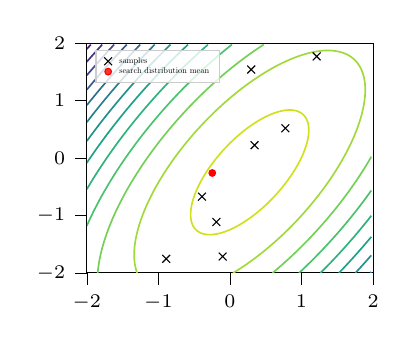
\begin{tikzpicture}

\definecolor{color0}{rgb}{0.28291,0.105393,0.426902}
\definecolor{color1}{rgb}{0.275191,0.194905,0.496005}
\definecolor{color2}{rgb}{0.248629,0.278775,0.534556}
\definecolor{color3}{rgb}{0.212395,0.359683,0.55171}
\definecolor{color4}{rgb}{0.180629,0.429975,0.557282}
\definecolor{color5}{rgb}{0.153364,0.497,0.557724}
\definecolor{color6}{rgb}{0.127568,0.566949,0.550556}
\definecolor{color7}{rgb}{0.122312,0.633153,0.530398}
\definecolor{color8}{rgb}{0.175707,0.6979,0.491033}
\definecolor{color9}{rgb}{0.288921,0.758394,0.428426}
\definecolor{color10}{rgb}{0.449368,0.813768,0.335384}
\definecolor{color11}{rgb}{0.626579,0.854645,0.223353}
\definecolor{color12}{rgb}{0.814576,0.883393,0.110347}
\definecolor{color13}{rgb}{0.12156862745098,0.466666666666667,0.705882352941177}

\begin{axis}[
legend cell align={left},
legend style={
  fill opacity=0.8,
  draw opacity=1,
  text opacity=1,
  at={(0.03,0.97)},
  anchor=north west,
  draw=white!80!black,
  nodes={scale=0.3, transform shape}  
},
tick align=outside,
tick pos=left,
height=4.5cm,
ticklabel style = {font=\scriptsize},
x grid style={white!69.0196078431373!black},
xmin=-2, xmax=2,
xtick style={color=black},
y grid style={white!69.0196078431373!black},
ymin=-2, ymax=2,
ytick style={color=black}
]
\addplot [draw=black, fill=black, mark=x, only marks,]
table{%
x  y
0.297465961519502 1.54053155658749
-0.188820157315861 -1.11297999757822
-0.390747550879801 -0.672401256433344
-0.101996206751346 -1.71498354836645
1.21145597079931 1.76898302107758
0.774242934490292 0.517821828039633
0.343456999574768 0.223553213892614
-0.89050917853105 -1.7539639832343
-2.60614047231525 -2.7645768447781
-1.44907475370391 -2.01742939465281
};
\addlegendentry{$~$ samples}
\addplot [draw=red, fill=red, only marks, mark=*,
mark options={scale=0.6}]
table{%
x  y
-0.247316845794121 -0.259789935392427
};
\addlegendentry{$~$ search distribution mean}
\path [draw=color0, semithick]
(axis cs:-1.94389919909354,1.97499999999999)
--(axis cs:-1.95,1.96656011713952)
--(axis cs:-1.96192751718835,1.94999999999999)
--(axis cs:-1.975,1.93183821670244)
--(axis cs:-1.97990438181187,1.92499999999999)
--(axis cs:-1.99781425186483,1.89999999999999)
--(axis cs:-2,1.89694373222127);

\path [draw=color1, semithick]
(axis cs:-1.78527152175681,1.97499999999999)
--(axis cs:-1.8,1.95489438423099)
--(axis cs:-1.8035719208045,1.94999999999999)
--(axis cs:-1.82179163537837,1.92499999999999)
--(axis cs:-1.825,1.92059117906985)
--(axis cs:-1.83992812790451,1.89999999999999)
--(axis cs:-1.85,1.88609776546614)
--(axis cs:-1.8580099564479,1.87499999999999)
--(axis cs:-1.875,1.85144415835056)
--(axis cs:-1.87603773342439,1.84999999999999)
--(axis cs:-1.89396574555094,1.82499999999999)
--(axis cs:-1.9,1.81657766488979)
--(axis cs:-1.9118328456199,1.79999999999999)
--(axis cs:-1.925,1.7815401947262)
--(axis cs:-1.92964768077245,1.77499999999999)
--(axis cs:-1.94739087528784,1.74999999999999)
--(axis cs:-1.95,1.74631736880696)
--(axis cs:-1.96504702451655,1.72499999999999)
--(axis cs:-1.975,1.71088960232866)
--(axis cs:-1.98265265504473,1.69999999999999)
--(axis cs:-2,1.67529775307578);

\path [draw=color2, semithick]
(axis cs:-1.61838932225971,1.97499999999999)
--(axis cs:-1.625,1.96612763593603)
--(axis cs:-1.63696868392949,1.94999999999999)
--(axis cs:-1.65,1.93242801117585)
--(axis cs:-1.65548675837124,1.92499999999999)
--(axis cs:-1.67393560547545,1.89999999999999)
--(axis cs:-1.675,1.89855479125432)
--(axis cs:-1.69227932627487,1.87499999999999)
--(axis cs:-1.7,1.86446781657045)
--(axis cs:-1.71056384680711,1.84999999999999)
--(axis cs:-1.725,1.83021466700925)
--(axis cs:-1.72878986536019,1.82499999999999)
--(axis cs:-1.7469332913073,1.79999999999999)
--(axis cs:-1.75,1.79576759331277)
--(axis cs:-1.76498856169846,1.77499999999999)
--(axis cs:-1.775,1.76111850810879)
--(axis cs:-1.7829873409435,1.74999999999999)
--(axis cs:-1.8,1.72630099147479)
--(axis cs:-1.80093029033916,1.72499999999999)
--(axis cs:-1.81876808823417,1.69999999999999)
--(axis cs:-1.825,1.69125760565912)
--(axis cs:-1.83654380837669,1.67499999999999)
--(axis cs:-1.85,1.65603530587854)
--(axis cs:-1.85426563648644,1.64999999999999)
--(axis cs:-1.87190950647297,1.62499999999999)
--(axis cs:-1.875,1.62061339538621)
--(axis cs:-1.88946627449185,1.59999999999999)
--(axis cs:-1.9,1.58497918172269)
--(axis cs:-1.90697104240908,1.57499999999999)
--(axis cs:-1.9244197932592,1.54999999999999)
--(axis cs:-1.925,1.54916670724662)
--(axis cs:-1.94176164437002,1.52499999999999)
--(axis cs:-1.95,1.51311326013227)
--(axis cs:-1.95905334247659,1.49999999999999)
--(axis cs:-1.975,1.47688504797808)
--(axis cs:-1.97629546607764,1.47499999999999)
--(axis cs:-1.99343672318144,1.44999999999999)
--(axis cs:-2,1.44041754486338);

\path [draw=color3, semithick]
(axis cs:-1.44179034981397,1.97499999999999)
--(axis cs:-1.45,1.96418575082279)
--(axis cs:-1.46072368250311,1.94999999999999)
--(axis cs:-1.475,1.93110070005729)
--(axis cs:-1.47958903350432,1.92499999999999)
--(axis cs:-1.49837321150327,1.89999999999999)
--(axis cs:-1.5,1.89783090379435)
--(axis cs:-1.51705084754739,1.87499999999999)
--(axis cs:-1.525,1.86434823100687)
--(axis cs:-1.53566290918089,1.84999999999999)
--(axis cs:-1.55,1.83069331511346)
--(axis cs:-1.55421021643866,1.82499999999999)
--(axis cs:-1.57267365284374,1.79999999999999)
--(axis cs:-1.575,1.79684449061399)
--(axis cs:-1.59103734104118,1.77499999999999)
--(axis cs:-1.6,1.76278275906324)
--(axis cs:-1.60933858940764,1.74999999999999)
--(axis cs:-1.625,1.72854635184362)
--(axis cs:-1.62757817252472,1.72499999999999)
--(axis cs:-1.64572049476179,1.69999999999999)
--(axis cs:-1.65,1.69409468982585)
--(axis cs:-1.66378045063444,1.67499999999999)
--(axis cs:-1.675,1.65944198106232)
--(axis cs:-1.68178096707881,1.64999999999999)
--(axis cs:-1.69972040940485,1.62499999999999)
--(axis cs:-1.7,1.62460942140685)
--(axis cs:-1.71754375085731,1.59999999999999)
--(axis cs:-1.725,1.58953276824095)
--(axis cs:-1.73530982319682,1.57499999999999)
--(axis cs:-1.75,1.55427679683209)
--(axis cs:-1.7530193285173,1.54999999999999)
--(axis cs:-1.77063631851287,1.52499999999999)
--(axis cs:-1.775,1.51879814611954)
--(axis cs:-1.7881724842043,1.49999999999999)
--(axis cs:-1.8,1.48310818024594)
--(axis cs:-1.80565417050861,1.47499999999999)
--(axis cs:-1.82306586207867,1.44999999999999)
--(axis cs:-1.825,1.44721684063874)
--(axis cs:-1.84037657525514,1.42499999999999)
--(axis cs:-1.85,1.4110847572299)
--(axis cs:-1.85763484468407,1.39999999999999)
--(axis cs:-1.87483997236222,1.37499999999999)
--(axis cs:-1.875,1.37476684031496)
--(axis cs:-1.89192960557725,1.34999999999999)
--(axis cs:-1.9,1.33818428764706)
--(axis cs:-1.90896877994162,1.32499999999999)
--(axis cs:-1.925,1.30141523620853)
--(axis cs:-1.92595810457255,1.29999999999999)
--(axis cs:-1.94283897066729,1.27499999999999)
--(axis cs:-1.95,1.26438375309326)
--(axis cs:-1.95966329311746,1.24999999999999)
--(axis cs:-1.975,1.22715328165426)
--(axis cs:-1.97643967564236,1.22499999999999)
--(axis cs:-1.99311195443566,1.19999999999999)
--(axis cs:-2,1.18965932255347);

\path [draw=color4, semithick]
(axis cs:-1.25357422507695,1.97499999999999)
--(axis cs:-1.27294058800861,1.94999999999999)
--(axis cs:-1.275,1.94733707458173)
--(axis cs:-1.29219669506718,1.92499999999999)
--(axis cs:-1.3,1.91485627897205)
--(axis cs:-1.31137718042114,1.89999999999999)
--(axis cs:-1.325,1.88219753738268)
--(axis cs:-1.33048305933182,1.87499999999999)
--(axis cs:-1.3495108328669,1.84999999999999)
--(axis cs:-1.35,1.84935590748455)
--(axis cs:-1.36841470964074,1.82499999999999)
--(axis cs:-1.375,1.81628324245126)
--(axis cs:-1.3872467569008,1.79999999999999)
--(axis cs:-1.4,1.78303002137606)
--(axis cs:-1.4060079307089,1.77499999999999)
--(axis cs:-1.4246964036524,1.74999999999999)
--(axis cs:-1.425,1.74959293063851)
--(axis cs:-1.44326025091332,1.72499999999999)
--(axis cs:-1.45,1.71591570740983)
--(axis cs:-1.46175588812835,1.69999999999999)
--(axis cs:-1.475,1.68205524818943)
--(axis cs:-1.48018421544798,1.67499999999999)
--(axis cs:-1.49853286107407,1.64999999999999)
--(axis cs:-1.5,1.64799676923277)
--(axis cs:-1.5167684111648,1.62499999999999)
--(axis cs:-1.525,1.61370189180764)
--(axis cs:-1.53493920645576,1.59999999999999)
--(axis cs:-1.55,1.57922102588333)
--(axis cs:-1.55304609427973,1.57499999999999)
--(axis cs:-1.57105455849967,1.54999999999999)
--(axis cs:-1.575,1.5445140542411)
--(axis cs:-1.58897309643591,1.52499999999999)
--(axis cs:-1.6,1.50958800195885)
--(axis cs:-1.60683017862848,1.49999999999999)
--(axis cs:-1.62462324064948,1.47499999999999)
--(axis cs:-1.625,1.47446926119467)
--(axis cs:-1.64229469276336,1.44999999999999)
--(axis cs:-1.65,1.4390893247119)
--(axis cs:-1.65990707623191,1.42499999999999)
--(axis cs:-1.675,1.4035181338875)
--(axis cs:-1.6774611544142,1.39999999999999)
--(axis cs:-1.69491265996606,1.37499999999999)
--(axis cs:-1.7,1.36770144978615)
--(axis cs:-1.71228535242911,1.34999999999999)
--(axis cs:-1.725,1.33166492425641)
--(axis cs:-1.72960203074786,1.32499999999999)
--(axis cs:-1.74683552260931,1.29999999999999)
--(axis cs:-1.75,1.29539997118949)
--(axis cs:-1.76397343479257,1.27499999999999)
--(axis cs:-1.775,1.25888883058709)
--(axis cs:-1.78105756365705,1.24999999999999)
--(axis cs:-1.79807166811057,1.22499999999999)
--(axis cs:-1.8,1.22215958151434)
--(axis cs:-1.81497961588694,1.19999999999999)
--(axis cs:-1.825,1.1851642669782)
--(axis cs:-1.83183595238266,1.17499999999999)
--(axis cs:-1.84862934948648,1.14999999999999)
--(axis cs:-1.85,1.14795402993342)
--(axis cs:-1.86531205596172,1.12499999999999)
--(axis cs:-1.875,1.11046469292024)
--(axis cs:-1.88194526589412,1.09999999999999)
--(axis cs:-1.89851668803422,1.07499999999999)
--(axis cs:-1.9,1.07275607782477)
--(axis cs:-1.9149787855798,1.04999999999999)
--(axis cs:-1.925,1.03476256835592)
--(axis cs:-1.93139344546637,1.02499999999999)
--(axis cs:-1.94774167594889,0.999999999999989)
--(axis cs:-1.95,0.996537451868214)
--(axis cs:-1.96398770818355,0.974999999999989)
--(axis cs:-1.975,0.95802930617769)
--(axis cs:-1.98018830719594,0.94999999999999)
--(axis cs:-1.99631217887872,0.92499999999999)
--(axis cs:-2,0.919268794443722);

\path [draw=color5, semithick]
(axis cs:1.96298712893194,-2)
--(axis cs:1.97499999999999,-1.98348398736396);

\path [draw=color5, semithick]
(axis cs:-1.05107206095978,1.97499999999999)
--(axis cs:-1.07095011998956,1.94999999999999)
--(axis cs:-1.075,1.94490099855814)
--(axis cs:-1.09072923795155,1.92499999999999)
--(axis cs:-1.1,1.91326082015811)
--(axis cs:-1.11042159509316,1.89999999999999)
--(axis cs:-1.125,1.88143471482984)
--(axis cs:-1.13002844911795,1.87499999999999)
--(axis cs:-1.14954653478866,1.84999999999999)
--(axis cs:-1.15,1.84941791928042)
--(axis cs:-1.16893063329988,1.82499999999999)
--(axis cs:-1.175,1.81716488180767)
--(axis cs:-1.18823257968993,1.79999999999999)
--(axis cs:-1.2,1.78472305463585)
--(axis cs:-1.20745355381083,1.77499999999999)
--(axis cs:-1.225,1.75209196905912)
--(axis cs:-1.22659471302918,1.74999999999999)
--(axis cs:-1.24561428883865,1.72499999999999)
--(axis cs:-1.25,1.71922799261599)
--(axis cs:-1.26454026587646,1.69999999999999)
--(axis cs:-1.275,1.68615653493722)
--(axis cs:-1.28338958123879,1.67499999999999)
--(axis cs:-1.3,1.6528928633722)
--(axis cs:-1.30216332065958,1.64999999999999)
--(axis cs:-1.3208220499821,1.62499999999999)
--(axis cs:-1.325,1.61939415400849)
--(axis cs:-1.33938590517879,1.59999999999999)
--(axis cs:-1.35,1.5856786864809)
--(axis cs:-1.35787720063789,1.57499999999999)
--(axis cs:-1.375,1.55176796526766)
--(axis cs:-1.37629695468716,1.54999999999999)
--(axis cs:-1.39459423786676,1.52499999999999)
--(axis cs:-1.4,1.51760507297185)
--(axis cs:-1.41280925351013,1.49999999999999)
--(axis cs:-1.425,1.4832307243179)
--(axis cs:-1.43095561361059,1.47499999999999)
--(axis cs:-1.44902494718712,1.44999999999999)
--(axis cs:-1.45,1.44864757854114)
--(axis cs:-1.46696971813009,1.42499999999999)
--(axis cs:-1.475,1.41380004332482)
--(axis cs:-1.48484863834303,1.39999999999999)
--(axis cs:-1.5,1.37875142787097)
--(axis cs:-1.50266261973707,1.37499999999999)
--(axis cs:-1.52036865534375,1.34999999999999)
--(axis cs:-1.525,1.34345024534083)
--(axis cs:-1.53798596599824,1.32499999999999)
--(axis cs:-1.55,1.30791581953938)
--(axis cs:-1.55554102229358,1.29999999999999)
--(axis cs:-1.57301595184105,1.27499999999999)
--(axis cs:-1.575,1.27215465998066)
--(axis cs:-1.59037736246654,1.24999999999999)
--(axis cs:-1.6,1.23612418739021)
--(axis cs:-1.60767912791203,1.22499999999999)
--(axis cs:-1.62492132390798,1.19999999999999)
--(axis cs:-1.625,1.19988557490715)
--(axis cs:-1.64203242608698,1.17499999999999)
--(axis cs:-1.65,1.16334849432039)
--(axis cs:-1.65908641902368,1.14999999999999)
--(axis cs:-1.675,1.12660125497537)
--(axis cs:-1.67608407990407,1.12499999999999)
--(axis cs:-1.69296059122516,1.09999999999999)
--(axis cs:-1.7,1.08955959608651)
--(axis cs:-1.70977221680156,1.07499999999999)
--(axis cs:-1.725,1.05229184508452)
--(axis cs:-1.72652993830881,1.04999999999999)
--(axis cs:-1.74317113176002,1.02499999999999)
--(axis cs:-1.75,1.01472718611097)
--(axis cs:-1.75974568457395,0.999999999999989)
--(axis cs:-1.775,0.976927590245976)
--(axis cs:-1.77626869321018,0.974999999999989)
--(axis cs:-1.79267316448181,0.94999999999999)
--(axis cs:-1.8,0.938819736952899)
--(axis cs:-1.8090158311514,0.92499999999999)
--(axis cs:-1.825,0.900476591481389)
--(axis cs:-1.82530924726372,0.89999999999999)
--(axis cs:-1.84147565240424,0.87499999999999)
--(axis cs:-1.85,0.861804438206597)
--(axis cs:-1.8575915140701,0.84999999999999)
--(axis cs:-1.87364791234682,0.82499999999999)
--(axis cs:-1.875,0.822888044930224)
--(axis cs:-1.88958740799314,0.79999999999999)
--(axis cs:-1.9,0.78364713057017)
--(axis cs:-1.90548144275378,0.77499999999999)
--(axis cs:-1.92129668623862,0.74999999999999)
--(axis cs:-1.925,0.744130772850161)
--(axis cs:-1.93701709631404,0.72499999999999)
--(axis cs:-1.95,0.704312235806189)
--(axis cs:-1.95269418159667,0.69999999999999)
--(axis cs:-1.96826707399397,0.67499999999999)
--(axis cs:-1.975,0.66417210790989)
--(axis cs:-1.98377323810125,0.649999999999991)
--(axis cs:-1.99923113453546,0.624999999999991)
--(axis cs:-2,0.623751960811101);

\path [draw=color6, semithick]
(axis cs:1.7531783428001,-2)
--(axis cs:1.77178856562892,-1.975)
--(axis cs:1.77499999999999,-1.97067800427796)
--(axis cs:1.79028670824824,-1.95)
--(axis cs:1.79999999999999,-1.93684908528328)
--(axis cs:1.80870757287494,-1.925)
--(axis cs:1.82499999999999,-1.90280941569063)
--(axis cs:1.82705232409144,-1.9)
--(axis cs:1.8452733641571,-1.875)
--(axis cs:1.84999999999999,-1.86850497882114)
--(axis cs:1.86339899918361,-1.85)
--(axis cs:1.87499999999999,-1.8339634501108)
--(axis cs:1.8814518295486,-1.825)
--(axis cs:1.8994270614912,-1.8)
--(axis cs:1.89999999999999,-1.79920088327701)
--(axis cs:1.91726439981836,-1.775)
--(axis cs:1.92499999999999,-1.76414631815844)
--(axis cs:1.93503214237358,-1.75)
--(axis cs:1.94999999999999,-1.72887420346082)
--(axis cs:1.952731323042,-1.725)
--(axis cs:1.970315333128,-1.7)
--(axis cs:1.97499999999999,-1.69332785549737);

\path [draw=color6, semithick]
(axis cs:-0.830406972510627,1.97499999999999)
--(axis cs:-0.850000000000004,1.9512195838903)
--(axis cs:-0.850999472095394,1.94999999999999)
--(axis cs:-0.871449651419609,1.92499999999999)
--(axis cs:-0.875000000000004,1.92065477371954)
--(axis cs:-0.891786306612968,1.89999999999999)
--(axis cs:-0.900000000000004,1.8898846353684)
--(axis cs:-0.912022191064673,1.87499999999999)
--(axis cs:-0.925000000000004,1.85891822265396)
--(axis cs:-0.93215890107383,1.84999999999999)
--(axis cs:-0.950000000000004,1.82775502227949)
--(axis cs:-0.952197999400887,1.82499999999999)
--(axis cs:-0.972109861507093,1.79999999999999)
--(axis cs:-0.975000000000004,1.79636589210791)
--(axis cs:-0.991902616465261,1.77499999999999)
--(axis cs:-1,1.76475542608894)
--(axis cs:-1.01160183337517,1.74999999999999)
--(axis cs:-1.025,1.73294495231143)
--(axis cs:-1.03120897133582,1.72499999999999)
--(axis cs:-1.05,1.7009339417062)
--(axis cs:-1.0507254592559,1.69999999999999)
--(axis cs:-1.07010068198756,1.67499999999999)
--(axis cs:-1.075,1.66867143799678)
--(axis cs:-1.08937988082046,1.64999999999999)
--(axis cs:-1.1,1.63619811523367)
--(axis cs:-1.10857224318554,1.62499999999999)
--(axis cs:-1.125,1.60352092446394)
--(axis cs:-1.1276791032693,1.59999999999999)
--(axis cs:-1.146666728956,1.57499999999999)
--(axis cs:-1.15,1.57060391677142)
--(axis cs:-1.16554260660324,1.54999999999999)
--(axis cs:-1.175,1.53745160745585)
--(axis cs:-1.18433661654164,1.52499999999999)
--(axis cs:-1.2,1.50409199768637)
--(axis cs:-1.20305000426059,1.49999999999999)
--(axis cs:-1.2216491100431,1.47499999999999)
--(axis cs:-1.225,1.47048779404513)
--(axis cs:-1.24013762593601,1.44999999999999)
--(axis cs:-1.25,1.43663977154189)
--(axis cs:-1.25854898462858,1.42499999999999)
--(axis cs:-1.275,1.402580910468)
--(axis cs:-1.27688434852931,1.39999999999999)
--(axis cs:-1.29509428650728,1.37499999999999)
--(axis cs:-1.3,1.36825512395797)
--(axis cs:-1.31321070082082,1.34999999999999)
--(axis cs:-1.325,1.33369404384216)
--(axis cs:-1.33125442468304,1.32499999999999)
--(axis cs:-1.34921852439565,1.29999999999999)
--(axis cs:-1.35,1.2989094100227)
--(axis cs:-1.36704691978035,1.27499999999999)
--(axis cs:-1.375,1.26383492231681)
--(axis cs:-1.38480582934048,1.24999999999999)
--(axis cs:-1.4,1.22854279189605)
--(axis cs:-1.40249628501843,1.22499999999999)
--(axis cs:-1.42006918898094,1.19999999999999)
--(axis cs:-1.425,1.19297333988991)
--(axis cs:-1.43754995778419,1.17499999999999)
--(axis cs:-1.45,1.15715299484397)
--(axis cs:-1.45496532983627,1.14999999999999)
--(axis cs:-1.47228884152007,1.12499999999999)
--(axis cs:-1.475,1.12107782621297)
--(axis cs:-1.48949799478861,1.09999999999999)
--(axis cs:-1.5,1.08471721920846)
--(axis cs:-1.5066447163271,1.07499999999999)
--(axis cs:-1.52371700107076,1.04999999999999)
--(axis cs:-1.525,1.04811557973857)
--(axis cs:-1.54066091945862,1.02499999999999)
--(axis cs:-1.55,1.01120224938974)
--(axis cs:-1.55754528170347,0.999999999999989)
--(axis cs:-1.57436458669677,0.974999999999989)
--(axis cs:-1.575,0.974052396580738)
--(axis cs:-1.59104950993536,0.94999999999999)
--(axis cs:-1.6,0.936573448370299)
--(axis cs:-1.60767766577554,0.92499999999999)
--(axis cs:-1.62424231753554,0.89999999999999)
--(axis cs:-1.625,0.898852594764012)
--(axis cs:-1.64067434797338,0.87499999999999)
--(axis cs:-1.65,0.860794680858056)
--(axis cs:-1.6570523154253,0.84999999999999)
--(axis cs:-1.67336071735317,0.82499999999999)
--(axis cs:-1.675,0.822478933508558)
--(axis cs:-1.68954582339324,0.79999999999999)
--(axis cs:-1.7,0.783828231388095)
--(axis cs:-1.70567948895976,0.77499999999999)
--(axis cs:-1.72173011897529,0.74999999999999)
--(axis cs:-1.725,0.744892527167756)
--(axis cs:-1.73767413841355,0.72499999999999)
--(axis cs:-1.75,0.705634716993064)
--(axis cs:-1.75356926034676,0.699999999999991)
--(axis cs:-1.76936066859805,0.67499999999999)
--(axis cs:-1.775,0.666052753400241)
--(axis cs:-1.78506931186622,0.649999999999991)
--(axis cs:-1.8,0.626172994017193)
--(axis cs:-1.80073152333705,0.624999999999991)
--(axis cs:-1.81626232998271,0.599999999999991)
--(axis cs:-1.825,0.585917155120715)
--(axis cs:-1.83174118329849,0.574999999999991)
--(axis cs:-1.8471480360298,0.549999999999991)
--(axis cs:-1.85,0.545357096626674)
--(axis cs:-1.8624448885377,0.524999999999991)
--(axis cs:-1.875,0.504441335732174)
--(axis cs:-1.87769941696542,0.499999999999991)
--(axis cs:-1.8928423626103,0.474999999999991)
--(axis cs:-1.9,0.463160130539809)
--(axis cs:-1.90791795529146,0.449999999999991)
--(axis cs:-1.92293332873878,0.424999999999991)
--(axis cs:-1.925,0.421546183108765)
--(axis cs:-1.93783133620599,0.399999999999991)
--(axis cs:-1.95,0.379544935018145)
--(axis cs:-1.95269097075968,0.374999999999992)
--(axis cs:-1.96743928513146,0.349999999999992)
--(axis cs:-1.975,0.337158200711093)
--(axis cs:-1.98212434506301,0.324999999999992)
--(axis cs:-1.99674152716081,0.299999999999992)
--(axis cs:-2,0.294407163318319);

\path [draw=color7, semithick]
(axis cs:1.52297092486033,-2)
--(axis cs:1.52499999999999,-1.99737154268563)
--(axis cs:1.54217273743701,-1.975)
--(axis cs:1.54999999999999,-1.96479322487137)
--(axis cs:1.56128091674972,-1.95)
--(axis cs:1.57499999999999,-1.93199196988197)
--(axis cs:1.58029702767269,-1.925)
--(axis cs:1.5992136124704,-1.9)
--(axis cs:1.59999999999999,-1.89895795660292)
--(axis cs:1.61797933153337,-1.875)
--(axis cs:1.62499999999999,-1.86563555731722)
--(axis cs:1.63665725611764,-1.85)
--(axis cs:1.64999999999999,-1.83208611278355)
--(axis cs:1.6552488378509,-1.825)
--(axis cs:1.67374126267309,-1.8)
--(axis cs:1.67499999999999,-1.79829375941618)
--(axis cs:1.69208965811834,-1.775)
--(axis cs:1.69999999999999,-1.76420720772164)
--(axis cs:1.71035576801079,-1.75)
--(axis cs:1.72499999999999,-1.72988936415054)
--(axis cs:1.72854093852043,-1.725)
--(axis cs:1.74660853870032,-1.7)
--(axis cs:1.74999999999999,-1.69529716083712)
--(axis cs:1.76455748724163,-1.675)
--(axis cs:1.77499999999999,-1.6604255732025)
--(axis cs:1.78242934938815,-1.65)
--(axis cs:1.79999999999999,-1.62531830182152)
--(axis cs:1.80022537307148,-1.625)
--(axis cs:1.8178678051702,-1.6)
--(axis cs:1.82499999999999,-1.58988235881844)
--(axis cs:1.83543434010322,-1.575)
--(axis cs:1.84999999999999,-1.55420399512693)
--(axis cs:1.85292869675287,-1.55)
--(axis cs:1.87030025194379,-1.525)
--(axis cs:1.87499999999999,-1.51822289948712)
--(axis cs:1.88756924765229,-1.5)
--(axis cs:1.89999999999999,-1.48195929053266)
--(axis cs:1.90476960540517,-1.475)
--(axis cs:1.92186808526476,-1.45)
--(axis cs:1.92499999999999,-1.44540867968465)
--(axis cs:1.93884714190171,-1.425)
--(axis cs:1.94999999999999,-1.40854514345448)
--(axis cs:1.95576098484647,-1.4)
--(axis cs:1.97258429721365,-1.375)
--(axis cs:1.97499999999999,-1.37139939132245);

\path [draw=color7, semithick]
(axis cs:-0.585639334873647,1.97499999999999)
--(axis cs:-0.600000000000005,1.95834636468364)
--(axis cs:-0.607154043722844,1.94999999999999)
--(axis cs:-0.625000000000005,1.92916046876722)
--(axis cs:-0.628541591612436,1.92499999999999)
--(axis cs:-0.649801816365295,1.89999999999999)
--(axis cs:-0.650000000000005,1.89976648890417)
--(axis cs:-0.670894311553601,1.87499999999999)
--(axis cs:-0.675000000000005,1.87012887948888)
--(axis cs:-0.691865355743964,1.84999999999999)
--(axis cs:-0.700000000000005,1.84028216440807)
--(axis cs:-0.712717095310544,1.82499999999999)
--(axis cs:-0.725000000000005,1.81022575510398)
--(axis cs:-0.733451626347228,1.79999999999999)
--(axis cs:-0.750000000000004,1.77995906080799)
--(axis cs:-0.75407099613137,1.77499999999999)
--(axis cs:-0.774572094421064,1.74999999999999)
--(axis cs:-0.775000000000004,1.74947705046334)
--(axis cs:-0.79491179092182,1.72499999999999)
--(axis cs:-0.800000000000004,1.71873926062771)
--(axis cs:-0.815141523759811,1.69999999999999)
--(axis cs:-0.825000000000004,1.68778748891483)
--(axis cs:-0.83526319224687,1.67499999999999)
--(axis cs:-0.850000000000004,1.65662112500933)
--(axis cs:-0.855278652204883,1.64999999999999)
--(axis cs:-0.875000000000004,1.62523955627265)
--(axis cs:-0.875189717203486,1.62499999999999)
--(axis cs:-0.894939067985897,1.59999999999999)
--(axis cs:-0.900000000000004,1.59358701600241)
--(axis cs:-0.914584788173563,1.57499999999999)
--(axis cs:-0.925000000000004,1.56171397315828)
--(axis cs:-0.934130853870427,1.54999999999999)
--(axis cs:-0.950000000000004,1.52962187299752)
--(axis cs:-0.953578948176298,1.52499999999999)
--(axis cs:-0.972906538160007,1.49999999999999)
--(axis cs:-0.975000000000004,1.4972864754655)
--(axis cs:-0.992097000423525,1.47499999999999)
--(axis cs:-1,1.46468816909459)
--(axis cs:-1.01119398830309,1.44999999999999)
--(axis cs:-1.025,1.43186682645841)
--(axis cs:-1.0301990634908,1.42499999999999)
--(axis cs:-1.04910351018495,1.39999999999999)
--(axis cs:-1.05,1.39881133296216)
--(axis cs:-1.06785840320312,1.37499999999999)
--(axis cs:-1.075,1.36546844485461)
--(axis cs:-1.08652565114992,1.34999999999999)
--(axis cs:-1.1,1.33189840912674)
--(axis cs:-1.10510670269924,1.32499999999999)
--(axis cs:-1.1235870018249,1.29999999999999)
--(axis cs:-1.125,1.29808348481934)
--(axis cs:-1.1419250694543,1.27499999999999)
--(axis cs:-1.15,1.2639759244204)
--(axis cs:-1.16018099206164,1.24999999999999)
--(axis cs:-1.175,1.22963696633419)
--(axis cs:-1.17835611307428,1.22499999999999)
--(axis cs:-1.1964116085525,1.19999999999999)
--(axis cs:-1.2,1.19502104178188)
--(axis cs:-1.2143507029571,1.17499999999999)
--(axis cs:-1.225,1.16012790490234)
--(axis cs:-1.23221284317559,1.14999999999999)
--(axis cs:-1.24999926642843,1.12499999999999)
--(axis cs:-1.25,1.12499896543307)
--(axis cs:-1.2676296308301,1.09999999999999)
--(axis cs:-1.275,1.08953809684661)
--(axis cs:-1.28518676214733,1.07499999999999)
--(axis cs:-1.3,1.05383762160132)
--(axis cs:-1.30267183958406,1.04999999999999)
--(axis cs:-1.32003129202393,1.02499999999999)
--(axis cs:-1.325,1.01783066498493)
--(axis cs:-1.33729119344874,0.999999999999989)
--(axis cs:-1.35,0.981544475798048)
--(axis cs:-1.3544825762495,0.974999999999989)
--(axis cs:-1.37156893080343,0.94999999999999)
--(axis cs:-1.375,0.944967035071016)
--(axis cs:-1.38853919377605,0.92499999999999)
--(axis cs:-1.4,0.908080433385323)
--(axis cs:-1.40544435749718,0.89999999999999)
--(axis cs:-1.4222555261667,0.87499999999999)
--(axis cs:-1.425,0.870906837035951)
--(axis cs:-1.43894355970568,0.84999999999999)
--(axis cs:-1.45,0.833404567885115)
--(axis cs:-1.4555698011333,0.82499999999999)
--(axis cs:-1.47210379845327,0.79999999999999)
--(axis cs:-1.475,0.795607799251962)
--(axis cs:-1.48851683413984,0.77499999999999)
--(axis cs:-1.5,0.757474022991313)
--(axis cs:-1.5048712761498,0.74999999999999)
--(axis cs:-1.52112621575565,0.72499999999999)
--(axis cs:-1.525,0.719025635236428)
--(axis cs:-1.53727131256146,0.69999999999999)
--(axis cs:-1.55,0.680243897465056)
--(axis cs:-1.5533609088273,0.67499999999999)
--(axis cs:-1.56933500014115,0.649999999999991)
--(axis cs:-1.575,0.641113922157895)
--(axis cs:-1.58521904910497,0.624999999999991)
--(axis cs:-1.6,0.601667121692095)
--(axis cs:-1.60105058865936,0.599999999999991)
--(axis cs:-1.61674213369036,0.574999999999991)
--(axis cs:-1.625,0.561823970443608)
--(axis cs:-1.63237186244914,0.549999999999991)
--(axis cs:-1.64792983048569,0.524999999999991)
--(axis cs:-1.65,0.521660919728787)
--(axis cs:-1.6633593643588,0.499999999999991)
--(axis cs:-1.675,0.481104683718787)
--(axis cs:-1.67874134153818,0.474999999999991)
--(axis cs:-1.69401276517962,0.449999999999991)
--(axis cs:-1.7,0.44017417674884)
--(axis cs:-1.70919821166743,0.424999999999991)
--(axis cs:-1.72433173526977,0.399999999999991)
--(axis cs:-1.725,0.398891048800835)
--(axis cs:-1.73932225813489,0.374999999999992)
--(axis cs:-1.75,0.357167950763827)
--(axis cs:-1.75426997222809,0.349999999999992)
--(axis cs:-1.76911315415648,0.324999999999992)
--(axis cs:-1.775,0.315057636761533)
--(axis cs:-1.78386953790079,0.299999999999992)
--(axis cs:-1.79857057252015,0.274999999999992)
--(axis cs:-1.8,0.27255818338716)
--(axis cs:-1.81313722419186,0.249999999999992)
--(axis cs:-1.825,0.229606241082057)
--(axis cs:-1.82766561672394,0.224999999999992)
--(axis cs:-1.84207270671612,0.199999999999992)
--(axis cs:-1.85,0.186213726606157)
--(axis cs:-1.85641489089056,0.174999999999992)
--(axis cs:-1.87067566066549,0.149999999999992)
--(axis cs:-1.875,0.142391228412599)
--(axis cs:-1.88483322601474,0.124999999999992)
--(axis cs:-1.89894576080831,0.0999999999999925)
--(axis cs:-1.9,0.0981229749030638)
--(axis cs:-1.91292030008477,0.0749999999999926)
--(axis cs:-1.925,0.0533550265951228)
--(axis cs:-1.92686280059241,0.0499999999999927)
--(axis cs:-1.94067579067105,0.0249999999999928)
--(axis cs:-1.95,0.00809087097623054)
--(axis cs:-1.95443870867897,-7.105427357601e-15)
--(axis cs:-1.96809937492541,-0.025000000000007)
--(axis cs:-1.975,-0.0376669667319595)
--(axis cs:-1.9816842944561,-0.0500000000000069)
--(axis cs:-1.99519072958038,-0.0750000000000068)
--(axis cs:-2,-0.0839373078575987);

\path [draw=color8, semithick]
(axis cs:1.26491421687666,-2)
--(axis cs:1.27499999999999,-1.98748565411003)
--(axis cs:1.28499851395528,-1.975)
--(axis cs:1.29999999999999,-1.95624711392572)
--(axis cs:1.30496576231271,-1.95)
--(axis cs:1.32481577999674,-1.925)
--(axis cs:1.32499999999999,-1.92476734310343)
--(axis cs:1.34448675408125,-1.9)
--(axis cs:1.34999999999999,-1.89298527483105)
--(axis cs:1.36404657528135,-1.875)
--(axis cs:1.37499999999999,-1.86096021588166)
--(axis cs:1.38349733019587,-1.85)
--(axis cs:1.39999999999999,-1.82869138638286)
--(axis cs:1.4028410535213,-1.825)
--(axis cs:1.42204201594935,-1.8)
--(axis cs:1.42499999999999,-1.79614068635813)
--(axis cs:1.44110255030407,-1.775)
--(axis cs:1.44999999999999,-1.76330608663982)
--(axis cs:1.46006149816235,-1.75)
--(axis cs:1.47499999999999,-1.73022278382633)
--(axis cs:1.47892073212519,-1.725)
--(axis cs:1.49765250297464,-1.7)
--(axis cs:1.49999999999999,-1.69685920287109)
--(axis cs:1.51623759413933,-1.675)
--(axis cs:1.52499999999999,-1.66319102746754)
--(axis cs:1.5347281102333,-1.65)
--(axis cs:1.54999999999999,-1.62926903333668)
--(axis cs:1.55312577410717,-1.625)
--(axis cs:1.57138728257346,-1.6)
--(axis cs:1.57499999999999,-1.59504318711843)
--(axis cs:1.58951951300018,-1.575)
--(axis cs:1.59999999999999,-1.56051632852546)
--(axis cs:1.60756374308125,-1.55)
--(axis cs:1.62499999999999,-1.52573034274766)
--(axis cs:1.6255215572614,-1.525)
--(axis cs:1.64331218991332,-1.5)
--(axis cs:1.64999999999999,-1.4905897152995)
--(axis cs:1.66101295892498,-1.475)
--(axis cs:1.67499999999999,-1.45517792932871)
--(axis cs:1.67863189488225,-1.45)
--(axis cs:1.69612300216947,-1.425)
--(axis cs:1.69999999999999,-1.41944493676553)
--(axis cs:1.71349001480655,-1.4)
--(axis cs:1.72499999999999,-1.38339021435593)
--(axis cs:1.73077961107442,-1.375)
--(axis cs:1.74796843353918,-1.35)
--(axis cs:1.74999999999999,-1.34703548304345)
--(axis cs:1.7650111346728,-1.325)
--(axis cs:1.77499999999999,-1.31031997919304)
--(axis cs:1.78198067578463,-1.3)
--(axis cs:1.79886460086851,-1.275)
--(axis cs:1.79999999999999,-1.27331244605213)
--(axis cs:1.81559218346196,-1.25)
--(axis cs:1.82499999999999,-1.23591756760781)
--(axis cs:1.83225070764592,-1.225)
--(axis cs:1.84882726423215,-1.2)
--(axis cs:1.84999999999999,-1.19822436291703)
--(axis cs:1.86524867697941,-1.175)
--(axis cs:1.87499999999999,-1.1601307264185)
--(axis cs:1.88160498358519,-1.15)
--(axis cs:1.89787183675115,-1.125)
--(axis cs:1.89999999999999,-1.12171704694555)
--(axis cs:1.9139957914491,-1.1)
--(axis cs:1.92499999999999,-1.08290443347396)
--(axis cs:1.93005844811724,-1.075)
--(axis cs:1.94601339408828,-1.05)
--(axis cs:1.94999999999999,-1.04373340500344)
--(axis cs:1.9618483727532,-1.025)
--(axis cs:1.97499999999999,-1.0041807117766);

\path [draw=color8, semithick]
(axis cs:-0.306572611053638,1.97499999999999)
--(axis cs:-0.325000000000006,1.95491214932371)
--(axis cs:-0.329474845195439,1.94999999999999)
--(axis cs:-0.350000000000006,1.92744627950773)
--(axis cs:-0.352210911495525,1.92499999999999)
--(axis cs:-0.374781131387378,1.89999999999999)
--(axis cs:-0.375000000000006,1.899757146464)
--(axis cs:-0.397158245166437,1.87499999999999)
--(axis cs:-0.400000000000006,1.87182169940457)
--(axis cs:-0.419377447564662,1.84999999999999)
--(axis cs:-0.425000000000006,1.84366175379905)
--(axis cs:-0.441441959962991,1.82499999999999)
--(axis cs:-0.450000000000006,1.81527662067821)
--(axis cs:-0.463354916712903,1.79999999999999)
--(axis cs:-0.475000000000005,1.7866656082507)
--(axis cs:-0.485119368055711,1.77499999999999)
--(axis cs:-0.500000000000005,1.75782802188866)
--(axis cs:-0.506738282925119,1.74999999999999)
--(axis cs:-0.525000000000005,1.7287631641131)
--(axis cs:-0.528214551638477,1.72499999999999)
--(axis cs:-0.549544812801781,1.69999999999999)
--(axis cs:-0.550000000000005,1.69946537653805)
--(axis cs:-0.570692271614234,1.67499999999999)
--(axis cs:-0.575000000000005,1.66990149848193)
--(axis cs:-0.591704167112524,1.64999999999999)
--(axis cs:-0.600000000000005,1.64010599964391)
--(axis cs:-0.612583157465212,1.62499999999999)
--(axis cs:-0.625000000000005,1.61007815734756)
--(axis cs:-0.633331831795861,1.59999999999999)
--(axis cs:-0.650000000000005,1.57981724590691)
--(axis cs:-0.653952712410344,1.57499999999999)
--(axis cs:-0.674440862379668,1.54999999999999)
--(axis cs:-0.675000000000005,1.54931610147959)
--(axis cs:-0.694751896652711,1.52499999999999)
--(axis cs:-0.700000000000005,1.51853237723239)
--(axis cs:-0.714941518257707,1.49999999999999)
--(axis cs:-0.725000000000005,1.4875110342226)
--(axis cs:-0.735012048168663,1.47499999999999)
--(axis cs:-0.750000000000004,1.45625132008254)
--(axis cs:-0.754965748575914,1.44999999999999)
--(axis cs:-0.774802257934874,1.42499999999999)
--(axis cs:-0.775000000000004,1.42475009542366)
--(axis cs:-0.794459963677677,1.39999999999999)
--(axis cs:-0.800000000000004,1.39294639750742)
--(axis cs:-0.814006725933933,1.37499999999999)
--(axis cs:-0.825000000000004,1.36089959070354)
--(axis cs:-0.833444626582761,1.34999999999999)
--(axis cs:-0.850000000000004,1.32860889452889)
--(axis cs:-0.852775695737848,1.32499999999999)
--(axis cs:-0.871963209355239,1.29999999999999)
--(axis cs:-0.875000000000004,1.29603517681328)
--(axis cs:-0.891011353536392,1.27499999999999)
--(axis cs:-0.900000000000004,1.26317823091164)
--(axis cs:-0.909958102383776,1.24999999999999)
--(axis cs:-0.925000000000004,1.23007245876522)
--(axis cs:-0.928805324279456,1.22499999999999)
--(axis cs:-0.947523654074116,1.19999999999999)
--(axis cs:-0.950000000000004,1.19668456425232)
--(axis cs:-0.966096986916231,1.17499999999999)
--(axis cs:-0.975000000000004,1.16299341849737)
--(axis cs:-0.984575923278704,1.14999999999999)
--(axis cs:-1,1.1290483263104)
--(axis cs:-1.00296218212679,1.12499999999999)
--(axis cs:-1.02121026962516,1.09999999999999)
--(axis cs:-1.025,1.09479679245865)
--(axis cs:-1.0393313390081,1.07499999999999)
--(axis cs:-1.05,1.06024631199512)
--(axis cs:-1.05736457493578,1.04999999999999)
--(axis cs:-1.075,1.02543657184466)
--(axis cs:-1.07531155827357,1.02499999999999)
--(axis cs:-1.09308880120558,0.999999999999989)
--(axis cs:-1.1,0.990268798821273)
--(axis cs:-1.11077897405576,0.974999999999989)
--(axis cs:-1.125,0.954832710486089)
--(axis cs:-1.12838746984538,0.94999999999999)
--(axis cs:-1.14586515190387,0.92499999999999)
--(axis cs:-1.15,0.919071455939927)
--(axis cs:-1.16322195391823,0.89999999999999)
--(axis cs:-1.175,0.882991862064007)
--(axis cs:-1.1805014885288,0.87499999999999)
--(axis cs:-1.19767685627477,0.84999999999999)
--(axis cs:-1.2,0.846607695028717)
--(axis cs:-1.21470972028277,0.82499999999999)
--(axis cs:-1.225,0.809866728375119)
--(axis cs:-1.2316695664831,0.79999999999999)
--(axis cs:-1.24854001311139,0.77499999999999)
--(axis cs:-1.25,0.772828524741334)
--(axis cs:-1.26525812043102,0.74999999999999)
--(axis cs:-1.275,0.73540756872069)
--(axis cs:-1.28190730506983,0.72499999999999)
--(axis cs:-1.29847036496246,0.69999999999999)
--(axis cs:-1.3,0.697682393748687)
--(axis cs:-1.31488265302423,0.67499999999999)
--(axis cs:-1.325,0.659562040180344)
--(axis cs:-1.33122996444287,0.649999999999991)
--(axis cs:-1.34748330793215,0.624999999999991)
--(axis cs:-1.35,0.62111502131468)
--(axis cs:-1.36359847763736,0.599999999999991)
--(axis cs:-1.375,0.582275025185446)
--(axis cs:-1.37965247282569,0.574999999999991)
--(axis cs:-1.3955939011581,0.549999999999991)
--(axis cs:-1.4,0.543069214236155)
--(axis cs:-1.41142042398198,0.524999999999991)
--(axis cs:-1.425,0.503488445198116)
--(axis cs:-1.42718943548744,0.499999999999991)
--(axis cs:-1.44281687598006,0.474999999999991)
--(axis cs:-1.45,0.463484668849201)
--(axis cs:-1.45836300082978,0.449999999999991)
--(axis cs:-1.47384142060767,0.424999999999991)
--(axis cs:-1.475,0.423120108979362)
--(axis cs:-1.48916664481069,0.399999999999991)
--(axis cs:-1.5,0.382297756660966)
--(axis cs:-1.50444040464789,0.374999999999992)
--(axis cs:-1.51959996315248,0.349999999999992)
--(axis cs:-1.525,0.341067322430139)
--(axis cs:-1.53465730971995,0.324999999999992)
--(axis cs:-1.54966255098813,0.299999999999992)
--(axis cs:-1.55,0.299434825414629)
--(axis cs:-1.56450545824636,0.274999999999992)
--(axis cs:-1.575,0.257298976782032)
--(axis cs:-1.57930267074357,0.249999999999992)
--(axis cs:-1.5939844492474,0.224999999999992)
--(axis cs:-1.6,0.214725050057343)
--(axis cs:-1.60857161357652,0.199999999999992)
--(axis cs:-1.62309388116177,0.174999999999992)
--(axis cs:-1.625,0.171702403421937)
--(axis cs:-1.63747295930824,0.149999999999992)
--(axis cs:-1.65,0.12817474202374)
--(axis cs:-1.65181184470171,0.124999999999992)
--(axis cs:-1.66600631021821,0.0999999999999925)
--(axis cs:-1.675,0.0841263656397908)
--(axis cs:-1.68014140637945,0.0749999999999926)
--(axis cs:-1.69417126801192,0.0499999999999927)
--(axis cs:-1.7,0.0395763901416526)
--(axis cs:-1.70810452502527,0.0249999999999928)
--(axis cs:-1.72196743381988,-7.105427357601e-15)
--(axis cs:-1.725,-0.0054959161665038)
--(axis cs:-1.73570080613959,-0.025000000000007)
--(axis cs:-1.74939440819656,-0.0500000000000069)
--(axis cs:-1.75,-0.0511124434284864)
--(axis cs:-1.76292985465638,-0.0750000000000068)
--(axis cs:-1.775,-0.0973303726580769)
--(axis cs:-1.77643483220021,-0.100000000000007)
--(axis cs:-1.78979127494209,-0.125000000000007)
--(axis cs:-1.8,-0.144147729877499)
--(axis cs:-1.80310249892578,-0.150000000000007)
--(axis cs:-1.81628467079468,-0.175000000000006)
--(axis cs:-1.825,-0.191575981912521)
--(axis cs:-1.82940408811976,-0.200000000000006)
--(axis cs:-1.84240964544256,-0.225000000000006)
--(axis cs:-1.85,-0.239641889270684)
--(axis cs:-1.85533920734665,-0.250000000000006)
--(axis cs:-1.8681658015436,-0.275000000000006)
--(axis cs:-1.875,-0.288373798627692)
--(axis cs:-1.88090746360986,-0.300000000000006)
--(axis cs:-1.89355274118406,-0.325000000000006)
--(axis cs:-1.9,-0.337801762115677)
--(axis cs:-1.90610846335063,-0.350000000000006)
--(axis cs:-1.91857006587761,-0.375000000000006)
--(axis cs:-1.925,-0.3879576675412)
--(axis cs:-1.93094181244711,-0.400000000000006)
--(axis cs:-1.94321737656428,-0.425000000000006)
--(axis cs:-1.95,-0.438875380719426)
--(axis cs:-1.95540711621329,-0.450000000000006)
--(axis cs:-1.96749427360941,-0.475000000000005)
--(axis cs:-1.975,-0.490590901260457)
--(axis cs:-1.97950397939801,-0.500000000000005)
--(axis cs:-1.99140035680265,-0.525000000000005)
--(axis cs:-2,-0.543142533314807);

\path [draw=color9, semithick]
(axis cs:0.96559519781874,-2)
--(axis cs:0.974999999999989,-1.98907457547417)
--(axis cs:0.987023943553011,-1.975)
--(axis cs:0.999999999999989,-1.95979309315398)
--(axis cs:1.00829367262852,-1.95)
--(axis cs:1.02499999999999,-1.93025012426433)
--(axis cs:1.02940794203489,-1.925)
--(axis cs:1.04999999999999,-1.90044474527996)
--(axis cs:1.0503702034601,-1.9)
--(axis cs:1.07112507701573,-1.875)
--(axis cs:1.07499999999999,-1.87032629269624)
--(axis cs:1.09172753877961,-1.85)
--(axis cs:1.09999999999999,-1.8399358159381)
--(axis cs:1.11218656303908,-1.825)
--(axis cs:1.12499999999999,-1.80927713558624)
--(axis cs:1.13250528954279,-1.8)
--(axis cs:1.14999999999999,-1.77834928963663)
--(axis cs:1.15268676706725,-1.775)
--(axis cs:1.17269983057966,-1.75)
--(axis cs:1.17499999999999,-1.74712018778738)
--(axis cs:1.19253984373599,-1.725)
--(axis cs:1.19999999999999,-1.71558030409982)
--(axis cs:1.21225042158564,-1.7)
--(axis cs:1.22499999999999,-1.68376518943209)
--(axis cs:1.23183433793788,-1.675)
--(axis cs:1.24999999999999,-1.65167384095286)
--(axis cs:1.2512942879068,-1.65)
--(axis cs:1.27056850339949,-1.625)
--(axis cs:1.27499999999999,-1.61924203562197)
--(axis cs:1.28970414508224,-1.6)
--(axis cs:1.29999999999999,-1.58651012434403)
--(axis cs:1.30872295574089,-1.575)
--(axis cs:1.32499999999999,-1.55349562394247)
--(axis cs:1.32762738762626,-1.55)
--(axis cs:1.34636776056904,-1.525)
--(axis cs:1.34999999999999,-1.52014337703153)
--(axis cs:1.36495966118398,-1.5)
--(axis cs:1.37499999999999,-1.48646366121098)
--(axis cs:1.38344386286208,-1.475)
--(axis cs:1.39999999999999,-1.45249473208876)
--(axis cs:1.40182259594836,-1.45)
--(axis cs:1.42002770351645,-1.425)
--(axis cs:1.42499999999999,-1.41815812385755)
--(axis cs:1.43810518414833,-1.4)
--(axis cs:1.44999999999999,-1.38349801598537)
--(axis cs:1.4560834530851,-1.375)
--(axis cs:1.4739497787085,-1.35)
--(axis cs:1.47499999999999,-1.34852486856392)
--(axis cs:1.49163363116998,-1.325)
--(axis cs:1.49999999999999,-1.31315225917775)
--(axis cs:1.50922427047685,-1.3)
--(axis cs:1.52499999999999,-1.27747748419723)
--(axis cs:1.52672358943615,-1.275)
--(axis cs:1.54405091432167,-1.25)
--(axis cs:1.54999999999999,-1.24139920973167)
--(axis cs:1.5612663672084,-1.225)
--(axis cs:1.57499999999999,-1.20498333959708)
--(axis cs:1.57839612232488,-1.2)
--(axis cs:1.59537819277548,-1.175)
--(axis cs:1.59999999999999,-1.16817721295705)
--(axis cs:1.61223052471952,-1.15)
--(axis cs:1.62499999999999,-1.13099662591448)
--(axis cs:1.62900254975641,-1.125)
--(axis cs:1.64563609186481,-1.1)
--(axis cs:1.64999999999999,-1.09342095926301)
--(axis cs:1.66213700364733,-1.075)
--(axis cs:1.67499999999999,-1.05545089403841)
--(axis cs:1.67856277684273,-1.05)
--(axis cs:1.6948447198146,-1.025)
--(axis cs:1.69999999999999,-1.01706120925482)
--(axis cs:1.71100556003946,-1)
--(axis cs:1.72499999999999,-0.978275691025614)
--(axis cs:1.7270962162332,-0.975000000000004)
--(axis cs:1.74302368384624,-0.950000000000004)
--(axis cs:1.74999999999999,-0.939024493639782)
--(axis cs:1.7588554609653,-0.925000000000004)
--(axis cs:1.77461661412577,-0.900000000000004)
--(axis cs:1.77499999999999,-0.899388598951369)
--(axis cs:1.79019210568434,-0.875000000000004)
--(axis cs:1.79999999999999,-0.859232785207053)
--(axis cs:1.80570549955128,-0.850000000000004)
--(axis cs:1.8211056221351,-0.825000000000004)
--(axis cs:1.82499999999999,-0.818652467186822)
--(axis cs:1.83636863649112,-0.800000000000004)
--(axis cs:1.84999999999999,-0.77760313980177)
--(axis cs:1.85157400946464,-0.775000000000004)
--(axis cs:1.86661069160129,-0.750000000000004)
--(axis cs:1.87499999999999,-0.736021497231235)
--(axis cs:1.88157147125278,-0.725000000000005)
--(axis cs:1.89643114154722,-0.700000000000005)
--(axis cs:1.89999999999999,-0.69396826645809)
--(axis cs:1.91114987906076,-0.675000000000005)
--(axis cs:1.92499999999999,-0.651403358328505)
--(axis cs:1.92581836264145,-0.650000000000005)
--(axis cs:1.94030871526145,-0.625000000000005)
--(axis cs:1.94999999999999,-0.608248200784494)
--(axis cs:1.95474080192191,-0.600000000000005)
--(axis cs:1.96904746137485,-0.575000000000005)
--(axis cs:1.97499999999999,-0.5645584892709);

\path [draw=color9, semithick]
(axis cs:0.027247685210488,1.97499999999999)
--(axis cs:0.0249999999999928,1.97279420459108)
--(axis cs:0.00197446976896861,1.94999999999999)
--(axis cs:-7.105427357601e-15,1.94804314090929)
--(axis cs:-0.0230504947836087,1.92499999999999)
--(axis cs:-0.025000000000007,1.92304889495602)
--(axis cs:-0.0478335608347291,1.89999999999999)
--(axis cs:-0.0500000000000069,1.89781063407707)
--(axis cs:-0.0723808658734343,1.87499999999999)
--(axis cs:-0.0750000000000068,1.87232752181256)
--(axis cs:-0.0966983415015099,1.84999999999999)
--(axis cs:-0.100000000000007,1.84659871787518)
--(axis cs:-0.120791721995012,1.82499999999999)
--(axis cs:-0.125000000000007,1.82062337812824)
--(axis cs:-0.144666552442095,1.79999999999999)
--(axis cs:-0.150000000000007,1.79440065456363)
--(axis cs:-0.168328196481402,1.77499999999999)
--(axis cs:-0.175000000000006,1.76792969527958)
--(axis cs:-0.191781843663713,1.74999999999999)
--(axis cs:-0.200000000000006,1.7412096444583)
--(axis cs:-0.215032516458063,1.72499999999999)
--(axis cs:-0.225000000000006,1.71423964234345)
--(axis cs:-0.238085076922215,1.69999999999999)
--(axis cs:-0.250000000000006,1.68701882521747)
--(axis cs:-0.260944233056099,1.67499999999999)
--(axis cs:-0.275000000000006,1.6595463253787)
--(axis cs:-0.283614544855647,1.64999999999999)
--(axis cs:-0.300000000000006,1.63182127111842)
--(axis cs:-0.306100430083387,1.62499999999999)
--(axis cs:-0.325000000000006,1.60384278669769)
--(axis cs:-0.32840616977114,1.59999999999999)
--(axis cs:-0.350000000000006,1.575609992324)
--(axis cs:-0.350535913469205,1.57499999999999)
--(axis cs:-0.372453656685938,1.54999999999999)
--(axis cs:-0.375000000000006,1.54709158291164)
--(axis cs:-0.394192786599394,1.52499999999999)
--(axis cs:-0.400000000000006,1.51830785501624)
--(axis cs:-0.415765816487634,1.49999999999999)
--(axis cs:-0.425000000000006,1.48926433749468)
--(axis cs:-0.437176516302821,1.47499999999999)
--(axis cs:-0.450000000000006,1.45996011467233)
--(axis cs:-0.458428542765586,1.44999999999999)
--(axis cs:-0.475000000000005,1.4303942665662)
--(axis cs:-0.479525443584524,1.42499999999999)
--(axis cs:-0.500000000000005,1.4005658688596)
--(axis cs:-0.500470661488393,1.39999999999999)
--(axis cs:-0.521210122467553,1.37499999999999)
--(axis cs:-0.525000000000005,1.37042529488855)
--(axis cs:-0.541795934214338,1.34999999999999)
--(axis cs:-0.550000000000005,1.34001124923672)
--(axis cs:-0.562238616914159,1.32499999999999)
--(axis cs:-0.575000000000005,1.30932885491568)
--(axis cs:-0.582541302180195,1.29999999999999)
--(axis cs:-0.600000000000005,1.27837714908211)
--(axis cs:-0.602707030928969,1.27499999999999)
--(axis cs:-0.622704717863506,1.24999999999999)
--(axis cs:-0.625000000000005,1.24712407225932)
--(axis cs:-0.642529350286397,1.22499999999999)
--(axis cs:-0.650000000000005,1.21555974627327)
--(axis cs:-0.662224824991189,1.19999999999999)
--(axis cs:-0.675000000000005,1.1837200374557)
--(axis cs:-0.681793908641704,1.17499999999999)
--(axis cs:-0.700000000000005,1.15160394208425)
--(axis cs:-0.701239289443046,1.14999999999999)
--(axis cs:-0.720498199016256,1.12499999999999)
--(axis cs:-0.725000000000005,1.11914616198861)
--(axis cs:-0.739619616198273,1.09999999999999)
--(axis cs:-0.750000000000004,1.08638888672633)
--(axis cs:-0.758624452541458,1.07499999999999)
--(axis cs:-0.775000000000004,1.05334886326347)
--(axis cs:-0.777515154009074,1.04999999999999)
--(axis cs:-0.796240228981912,1.02499999999999)
--(axis cs:-0.800000000000004,1.01996897090951)
--(axis cs:-0.814818728631366,0.999999999999989)
--(axis cs:-0.825000000000004,0.986263083362074)
--(axis cs:-0.833289760876257,0.974999999999989)
--(axis cs:-0.850000000000004,0.952267816722607)
--(axis cs:-0.85165555033693,0.94999999999999)
--(axis cs:-0.869845386174931,0.92499999999999)
--(axis cs:-0.875000000000004,0.917901777131171)
--(axis cs:-0.887910238243808,0.89999999999999)
--(axis cs:-0.900000000000004,0.883214649347265)
--(axis cs:-0.905876092961067,0.87499999999999)
--(axis cs:-0.923727091374079,0.84999999999999)
--(axis cs:-0.925000000000004,0.848210698968518)
--(axis cs:-0.941398836793267,0.82499999999999)
--(axis cs:-0.950000000000004,0.812810357657086)
--(axis cs:-0.958977572453758,0.79999999999999)
--(axis cs:-0.975000000000004,0.777107671388894)
--(axis cs:-0.976465186258623,0.77499999999999)
--(axis cs:-0.993777238891573,0.74999999999999)
--(axis cs:-1,0.740996578643773)
--(axis cs:-1.01098128058051,0.72499999999999)
--(axis cs:-1.025,0.704552047004184)
--(axis cs:-1.02809981282997,0.69999999999999)
--(axis cs:-1.04506657662042,0.67499999999999)
--(axis cs:-1.05,0.667711538803644)
--(axis cs:-1.06190797236945,0.649999999999991)
--(axis cs:-1.075,0.630501506340506)
--(axis cs:-1.07866923983499,0.624999999999991)
--(axis cs:-1.09528744912355,0.599999999999991)
--(axis cs:-1.1,0.592889801325056)
--(axis cs:-1.11177788291847,0.574999999999991)
--(axis cs:-1.125,0.554889470969046)
--(axis cs:-1.12819334747611,0.549999999999991)
--(axis cs:-1.14445993930199,0.524999999999991)
--(axis cs:-1.15,0.516461990448871)
--(axis cs:-1.16061074357471,0.499999999999991)
--(axis cs:-1.175,0.477645349318193)
--(axis cs:-1.17669152430586,0.474999999999991)
--(axis cs:-1.19260362988549,0.449999999999991)
--(axis cs:-1.2,0.438354490560627)
--(axis cs:-1.20842579751368,0.424999999999991)
--(axis cs:-1.22417147267424,0.399999999999991)
--(axis cs:-1.225,0.398677667189756)
--(axis cs:-1.23973761890737,0.374999999999992)
--(axis cs:-1.25,0.358489117270018)
--(axis cs:-1.25524181474367,0.349999999999992)
--(axis cs:-1.2706264606282,0.324999999999992)
--(axis cs:-1.275,0.317865798866654)
--(axis cs:-1.28588053460832,0.299999999999992)
--(axis cs:-1.3,0.276782757387313)
--(axis cs:-1.30107710656021,0.274999999999992)
--(axis cs:-1.31609831984722,0.249999999999992)
--(axis cs:-1.325,0.235155909286913)
--(axis cs:-1.33105054979366,0.224999999999992)
--(axis cs:-1.34589464751681,0.199999999999992)
--(axis cs:-1.35,0.193055946836137)
--(axis cs:-1.36060508487734,0.174999999999992)
--(axis cs:-1.375,0.150455474838454)
--(axis cs:-1.37526539566724,0.149999999999992)
--(axis cs:-1.38974019456881,0.124999999999992)
--(axis cs:-1.4,0.107251124106602)
--(axis cs:-1.40416435184366,0.0999999999999925)
--(axis cs:-1.41845536077374,0.0749999999999926)
--(axis cs:-1.425,0.0635104965516393)
--(axis cs:-1.43264589636997,0.0499999999999927)
--(axis cs:-1.44675006454416,0.0249999999999928)
--(axis cs:-1.45,0.0192087178695538)
--(axis cs:-1.46070951677548,-7.105427357601e-15)
--(axis cs:-1.47462378607666,-0.025000000000007)
--(axis cs:-1.475,-0.0256806487389246)
--(axis cs:-1.48835469975024,-0.0500000000000069)
--(axis cs:-1.5,-0.0712397379153075)
--(axis cs:-1.50204836946324,-0.0750000000000069)
--(axis cs:-1.51558093114335,-0.100000000000007)
--(axis cs:-1.525,-0.11744671633926)
--(axis cs:-1.52905151600609,-0.125000000000007)
--(axis cs:-1.54238769596124,-0.150000000000007)
--(axis cs:-1.55,-0.164323196848206)
--(axis cs:-1.55563772314383,-0.175000000000006)
--(axis cs:-1.56877447836587,-0.200000000000006)
--(axis cs:-1.575,-0.211902334765627)
--(axis cs:-1.58180648145866,-0.225000000000006)
--(axis cs:-1.59474076167312,-0.250000000000006)
--(axis cs:-1.6,-0.260219511400181)
--(axis cs:-1.60755728070256,-0.275000000000006)
--(axis cs:-1.62028602835092,-0.300000000000006)
--(axis cs:-1.625,-0.309312524045265)
--(axis cs:-1.63288960979561,-0.325000000000006)
--(axis cs:-1.64540976001763,-0.350000000000006)
--(axis cs:-1.65,-0.359221795777496)
--(axis cs:-1.65780295682429,-0.375000000000006)
--(axis cs:-1.67011143744022,-0.400000000000006)
--(axis cs:-1.675,-0.40999060750371)
--(axis cs:-1.68229680903977,-0.425000000000006)
--(axis cs:-1.69439054053254,-0.450000000000006)
--(axis cs:-1.7,-0.461665355058594)
--(axis cs:-1.70637065285622,-0.475000000000005)
--(axis cs:-1.71824654835357,-0.500000000000005)
--(axis cs:-1.725,-0.514295834565829)
--(axis cs:-1.73002397384906,-0.525000000000005)
--(axis cs:-1.74167893910568,-0.550000000000005)
--(axis cs:-1.75,-0.567935559755355)
--(axis cs:-1.75325625675333,-0.575000000000005)
--(axis cs:-1.76468719013284,-0.600000000000005)
--(axis cs:-1.775,-0.62264211549118)
--(axis cs:-1.77606698546189,-0.625000000000005)
--(axis cs:-1.78727077791888,-0.650000000000005)
--(axis cs:-1.79843470399224,-0.675000000000005)
--(axis cs:-1.8,-0.678539329932577)
--(axis cs:-1.80942917808568,-0.700000000000005)
--(axis cs:-1.82035961158402,-0.725000000000005)
--(axis cs:-1.825,-0.735699272024295)
--(axis cs:-1.83116186539144,-0.750000000000004)
--(axis cs:-1.84185563602826,-0.775000000000004)
--(axis cs:-1.85,-0.794156154395683)
--(axis cs:-1.85246831372889,-0.800000000000004)
--(axis cs:-1.86292224359219,-0.825000000000004)
--(axis cs:-1.87332541171721,-0.850000000000004)
--(axis cs:-1.875,-0.854068403910083)
--(axis cs:-1.88355889965707,-0.875000000000004)
--(axis cs:-1.89371559489128,-0.900000000000004)
--(axis cs:-1.9,-0.915594933753683)
--(axis cs:-1.90376506871633,-0.925000000000004)
--(axis cs:-1.91367204993275,-0.950000000000004)
--(axis cs:-1.92352009926349,-0.975000000000004)
--(axis cs:-1.925,-0.978802860946615)
--(axis cs:-1.93319423259509,-1)
--(axis cs:-1.94278570037691,-1.025)
--(axis cs:-1.95,-1.04396275659778)
--(axis cs:-1.95228159772082,-1.05)
--(axis cs:-1.96161317776884,-1.075)
--(axis cs:-1.97087711768698,-1.1)
--(axis cs:-1.975,-1.11125420629979)
--(axis cs:-1.98000197730515,-1.125)
--(axis cs:-1.98899891738124,-1.15)
--(axis cs:-1.99792287387805,-1.175)
--(axis cs:-2,-1.18090056289392);

\path [draw=color10, semithick]
(axis cs:0.595020075870905,-2)
--(axis cs:0.599999999999991,-1.99485313832505)
--(axis cs:0.61901933586069,-1.975)
--(axis cs:0.624999999999991,-1.9687486049244)
--(axis cs:0.642761097860865,-1.95)
--(axis cs:0.649999999999991,-1.94234815119469)
--(axis cs:0.666252849411239,-1.925)
--(axis cs:0.67499999999999,-1.91565055934181)
--(axis cs:0.689501790540949,-1.9)
--(axis cs:0.69999999999999,-1.8886546048804)
--(axis cs:0.712514847437233,-1.875)
--(axis cs:0.72499999999999,-1.8613590565878)
--(axis cs:0.735298685341745,-1.85)
--(axis cs:0.74999999999999,-1.8337626764577)
--(axis cs:0.757859720724864,-1.825)
--(axis cs:0.77499999999999,-1.80586421965331)
--(axis cs:0.780204132784718,-1.8)
--(axis cs:0.79999999999999,-1.77766243446019)
--(axis cs:0.802337874314226,-1.775)
--(axis cs:0.824252687903156,-1.75)
--(axis cs:0.82499999999999,-1.74914539010296)
--(axis cs:0.845920378727628,-1.725)
--(axis cs:0.84999999999999,-1.7202848746199)
--(axis cs:0.867391483723697,-1.7)
--(axis cs:0.87499999999999,-1.69111320349972)
--(axis cs:0.888671310878453,-1.675)
--(axis cs:0.89999999999999,-1.6616290637802)
--(axis cs:0.9097649787899,-1.65)
--(axis cs:0.92499999999999,-1.63183113510179)
--(axis cs:0.93067742503903,-1.625)
--(axis cs:0.949999999999989,-1.60171808965541)
--(axis cs:0.951413414121682,-1.6)
--(axis cs:0.971922385738465,-1.575)
--(axis cs:0.974999999999989,-1.57124064983149)
--(axis cs:0.992236310028096,-1.55)
--(axis cs:0.999999999999989,-1.54041894135576)
--(axis cs:1.01238561932415,-1.525)
--(axis cs:1.02499999999999,-1.50927373949906)
--(axis cs:1.03237456927775,-1.5)
--(axis cs:1.04999999999999,-1.47780364976113)
--(axis cs:1.05220727010301,-1.475)
--(axis cs:1.07183233202466,-1.45)
--(axis cs:1.07499999999999,-1.44595471364674)
--(axis cs:1.09126835533158,-1.425)
--(axis cs:1.09999999999999,-1.4137366451611)
--(axis cs:1.11055874348426,-1.4)
--(axis cs:1.12499999999999,-1.38118483720262)
--(axis cs:1.12970716852875,-1.375)
--(axis cs:1.14869473652679,-1.35)
--(axis cs:1.14999999999999,-1.34827501812043)
--(axis cs:1.16746369736775,-1.325)
--(axis cs:1.17499999999999,-1.31494094666124)
--(axis cs:1.18610050066749,-1.3)
--(axis cs:1.19999999999999,-1.28126383879462)
--(axis cs:1.20460842526947,-1.275)
--(axis cs:1.22295605587357,-1.25)
--(axis cs:1.22499999999999,-1.24720453985468)
--(axis cs:1.24110085866828,-1.225)
--(axis cs:1.24999999999999,-1.21270870833512)
--(axis cs:1.2591258488807,-1.2)
--(axis cs:1.27499999999999,-1.17786006583233)
--(axis cs:1.27703395220854,-1.175)
--(axis cs:1.29474039134214,-1.15)
--(axis cs:1.29999999999999,-1.14255498323488)
--(axis cs:1.31230089949362,-1.125)
--(axis cs:1.32499999999999,-1.10684879947484)
--(axis cs:1.32975290966598,-1.1)
--(axis cs:1.34705026575841,-1.075)
--(axis cs:1.34999999999999,-1.07071986592685)
--(axis cs:1.36416407308115,-1.05)
--(axis cs:1.37499999999999,-1.03412384789814)
--(axis cs:1.38117736017917,-1.025)
--(axis cs:1.39806070443561,-1)
--(axis cs:1.39999999999999,-0.997114740505791)
--(axis cs:1.41474494881713,-0.975000000000004)
--(axis cs:1.42499999999999,-0.959594749127648)
--(axis cs:1.43133625901278,-0.950000000000004)
--(axis cs:1.4478010208544,-0.925000000000004)
--(axis cs:1.44999999999999,-0.921644652507342)
--(axis cs:1.46407222327152,-0.900000000000004)
--(axis cs:1.47499999999999,-0.883164560074365)
--(axis cs:1.4802577042686,-0.875000000000004)
--(axis cs:1.49629965338024,-0.850000000000004)
--(axis cs:1.49999999999999,-0.844207731854868)
--(axis cs:1.51217374308627,-0.825000000000004)
--(axis cs:1.52499999999999,-0.80472926552803)
--(axis cs:1.52796896837073,-0.800000000000004)
--(axis cs:1.54358419767822,-0.775000000000004)
--(axis cs:1.54999999999999,-0.764694551596321)
--(axis cs:1.5590765362103,-0.750000000000004)
--(axis cs:1.57448831166162,-0.725000000000005)
--(axis cs:1.57499999999999,-0.724164413866019)
--(axis cs:1.58968143769768,-0.700000000000005)
--(axis cs:1.59999999999999,-0.682987413938002)
--(axis cs:1.60480684176693,-0.675000000000005)
--(axis cs:1.61978292634819,-0.650000000000005)
--(axis cs:1.62499999999999,-0.641252372563735)
--(axis cs:1.63461737529974,-0.625000000000005)
--(axis cs:1.64938025419827,-0.600000000000005)
--(axis cs:1.64999999999999,-0.598942886241687)
--(axis cs:1.66392739199382,-0.575000000000005)
--(axis cs:1.67499999999999,-0.555931001001742)
--(axis cs:1.67841725859649,-0.550000000000005)
--(axis cs:1.6927361536225,-0.525000000000005)
--(axis cs:1.69999999999999,-0.51226958595326)
--(axis cs:1.7069467264215,-0.500000000000005)
--(axis cs:1.72104292050665,-0.475000000000005)
--(axis cs:1.72499999999999,-0.467940214091656)
--(axis cs:1.73497781342151,-0.450000000000006)
--(axis cs:1.74884695151104,-0.425000000000006)
--(axis cs:1.74999999999999,-0.422905147185152)
--(axis cs:1.76250978949634,-0.400000000000006)
--(axis cs:1.77499999999999,-0.377087674181581)
--(axis cs:1.77612930751723,-0.375000000000006)
--(axis cs:1.78954192311903,-0.350000000000006)
--(axis cs:1.79999999999999,-0.33045607759901)
--(axis cs:1.80289712961422,-0.325000000000006)
--(axis cs:1.81607348133236,-0.300000000000006)
--(axis cs:1.82499999999999,-0.282999447378139)
--(axis cs:1.8291679712883,-0.275000000000006)
--(axis cs:1.84210372974536,-0.250000000000006)
--(axis cs:1.84999999999999,-0.234668281003849)
--(axis cs:1.85494110903517,-0.225000000000006)
--(axis cs:1.86763193252979,-0.200000000000006)
--(axis cs:1.87499999999999,-0.185409034897994)
--(axis cs:1.88021581794547,-0.175000000000006)
--(axis cs:1.89265735241664,-0.150000000000007)
--(axis cs:1.89999999999999,-0.135163703470936)
--(axis cs:1.90499137170138,-0.125000000000007)
--(axis cs:1.91717925069258,-0.100000000000007)
--(axis cs:1.92499999999999,-0.0838693444343982)
--(axis cs:1.92926704257318,-0.0750000000000068)
--(axis cs:1.94119688719643,-0.0500000000000069)
--(axis cs:1.94999999999999,-0.0314575421979419)
--(axis cs:1.95304210141585,-0.025000000000007)
--(axis cs:1.96470952031562,-7.105427357601e-15)
--(axis cs:1.97499999999999,0.0221462002825092);

\path [draw=color10, semithick]
(axis cs:0.471953469125981,1.97499999999999)
--(axis cs:0.449999999999991,1.95732604414606)
--(axis cs:0.441013562556946,1.94999999999999)
--(axis cs:0.424999999999991,1.93692760708243)
--(axis cs:0.410568801402624,1.92499999999999)
--(axis cs:0.399999999999991,1.91625292996277)
--(axis cs:0.380601107648807,1.89999999999999)
--(axis cs:0.374999999999992,1.89530089241876)
--(axis cs:0.351093272749854,1.87499999999999)
--(axis cs:0.349999999999992,1.87407036801526)
--(axis cs:0.324999999999992,1.85252926855023)
--(axis cs:0.322099988046315,1.84999999999999)
--(axis cs:0.299999999999992,1.83069947191526)
--(axis cs:0.293548658306255,1.82499999999999)
--(axis cs:0.274999999999992,1.80859108548745)
--(axis cs:0.265398693201971,1.79999999999999)
--(axis cs:0.249999999999992,1.78620298548884)
--(axis cs:0.23763659863519,1.77499999999999)
--(axis cs:0.224999999999992,1.76353404208918)
--(axis cs:0.210249478708961,1.74999999999999)
--(axis cs:0.199999999999992,1.74058311936518)
--(axis cs:0.183225002942727,1.72499999999999)
--(axis cs:0.174999999999992,1.71734907525931)
--(axis cs:0.156551375620183,1.69999999999999)
--(axis cs:0.149999999999992,1.69383076153838)
--(axis cs:0.130217307109799,1.67499999999999)
--(axis cs:0.124999999999992,1.67002702375172)
--(axis cs:0.104211987011443,1.64999999999999)
--(axis cs:0.0999999999999925,1.64593670118907)
--(axis cs:0.0785250589949038,1.62499999999999)
--(axis cs:0.0749999999999926,1.62155862683806)
--(axis cs:0.05314659720722,1.59999999999999)
--(axis cs:0.0499999999999927,1.59689162734139)
--(axis cs:0.0280670841358832,1.57499999999999)
--(axis cs:0.0249999999999928,1.57193452295366)
--(axis cs:0.00327738982416509,1.54999999999999)
--(axis cs:-7.105427357601e-15,1.54668612749786)
--(axis cs:-0.0212312476568109,1.52499999999999)
--(axis cs:-0.025000000000007,1.52114524832141)
--(axis cs:-0.0454672405670259,1.49999999999999)
--(axis cs:-0.0500000000000069,1.49531068625199)
--(axis cs:-0.0694386687683813,1.47499999999999)
--(axis cs:-0.0750000000000068,1.46918123555288)
--(axis cs:-0.09315329598188,1.44999999999999)
--(axis cs:-0.100000000000007,1.44275568387799)
--(axis cs:-0.116618585099909,1.42499999999999)
--(axis cs:-0.125000000000007,1.41603281222652)
--(axis cs:-0.139841712617077,1.39999999999999)
--(axis cs:-0.150000000000007,1.38901139489723)
--(axis cs:-0.162829582238254,1.37499999999999)
--(axis cs:-0.175000000000006,1.36169019944234)
--(axis cs:-0.185588837718004,1.34999999999999)
--(axis cs:-0.200000000000006,1.33406798662105)
--(axis cs:-0.208125874981617,1.32499999999999)
--(axis cs:-0.225000000000006,1.30614351035266)
--(axis cs:-0.23044685357418,1.29999999999999)
--(axis cs:-0.250000000000006,1.27791551766935)
--(axis cs:-0.252557707480761,1.27499999999999)
--(axis cs:-0.274453935437693,1.24999999999999)
--(axis cs:-0.275000000000006,1.24937494009828)
--(axis cs:-0.296099363823192,1.22499999999999)
--(axis cs:-0.300000000000006,1.22048748570264)
--(axis cs:-0.317548718582151,1.19999999999999)
--(axis cs:-0.325000000000006,1.19128867883478)
--(axis cs:-0.338807290988157,1.17499999999999)
--(axis cs:-0.350000000000006,1.16177720518978)
--(axis cs:-0.359880183623964,1.14999999999999)
--(axis cs:-0.375000000000006,1.13195174305488)
--(axis cs:-0.380772318718235,1.12499999999999)
--(axis cs:-0.400000000000006,1.10181096325724)
--(axis cs:-0.401488446044166,1.09999999999999)
--(axis cs:-0.421979034953028,1.07499999999999)
--(axis cs:-0.425000000000006,1.07130640696068)
--(axis cs:-0.44227364565379,1.04999999999999)
--(axis cs:-0.450000000000006,1.04045616566492)
--(axis cs:-0.462404063538304,1.02499999999999)
--(axis cs:-0.475000000000005,1.00928222042444)
--(axis cs:-0.482374531129798,0.999999999999989)
--(axis cs:-0.500000000000005,0.977783175275573)
--(axis cs:-0.502189146038105,0.974999999999989)
--(axis cs:-0.521795898346839,0.94999999999999)
--(axis cs:-0.525000000000005,0.945904395294954)
--(axis cs:-0.541214342174769,0.92499999999999)
--(axis cs:-0.550000000000005,0.913656516387448)
--(axis cs:-0.560487523404628,0.89999999999999)
--(axis cs:-0.575000000000005,0.881074675540329)
--(axis cs:-0.579619102825834,0.87499999999999)
--(axis cs:-0.598588358794654,0.84999999999999)
--(axis cs:-0.600000000000005,0.848132708066354)
--(axis cs:-0.61734095369835,0.82499999999999)
--(axis cs:-0.625000000000005,0.814767696599044)
--(axis cs:-0.635961730571288,0.79999999999999)
--(axis cs:-0.650000000000005,0.781059415073978)
--(axis cs:-0.654453958196784,0.77499999999999)
--(axis cs:-0.672783307051311,0.74999999999999)
--(axis cs:-0.675000000000005,0.746965472964511)
--(axis cs:-0.690912867536585,0.72499999999999)
--(axis cs:-0.700000000000005,0.712437504307836)
--(axis cs:-0.708922924991933,0.69999999999999)
--(axis cs:-0.725000000000005,0.677556479020714)
--(axis cs:-0.72681639611859,0.67499999999999)
--(axis cs:-0.744504612339655,0.649999999999991)
--(axis cs:-0.750000000000004,0.642214049331445)
--(axis cs:-0.762050919536236,0.624999999999991)
--(axis cs:-0.775000000000004,0.606474458261258)
--(axis cs:-0.779489011117287,0.599999999999991)
--(axis cs:-0.796768083872872,0.574999999999991)
--(axis cs:-0.800000000000004,0.570306063815366)
--(axis cs:-0.813868391079168,0.549999999999991)
--(axis cs:-0.825000000000004,0.533675559546866)
--(axis cs:-0.830868443200993,0.524999999999991)
--(axis cs:-0.8477334583994,0.499999999999991)
--(axis cs:-0.850000000000004,0.496624727252478)
--(axis cs:-0.864404873920216,0.474999999999991)
--(axis cs:-0.875000000000004,0.459069112284929)
--(axis cs:-0.88098360408801,0.449999999999991)
--(axis cs:-0.897430004976674,0.424999999999991)
--(axis cs:-0.900000000000004,0.421074863086356)
--(axis cs:-0.913689021518578,0.399999999999991)
--(axis cs:-0.925000000000004,0.38255794689783)
--(axis cs:-0.929862550031973,0.374999999999992)
--(axis cs:-0.945886119294366,0.349999999999992)
--(axis cs:-0.950000000000004,0.343554359801068)
--(axis cs:-0.961748639088203,0.324999999999992)
--(axis cs:-0.975000000000004,0.304037801914797)
--(axis cs:-0.9775325132298,0.299999999999992)
--(axis cs:-0.993129356009011,0.274999999999992)
--(axis cs:-1,0.263953527564282)
--(axis cs:-1.00861071475607,0.249999999999992)
--(axis cs:-1.02400394509084,0.224999999999992)
--(axis cs:-1.025,0.223371893500645)
--(axis cs:-1.03918645965264,0.199999999999992)
--(axis cs:-1.05,0.182154381895264)
--(axis cs:-1.05430144935707,0.174999999999992)
--(axis cs:-1.06925900210086,0.149999999999992)
--(axis cs:-1.075,0.140364662054084)
--(axis cs:-1.08408339418829,0.124999999999992)
--(axis cs:-1.09882759480528,0.0999999999999925)
--(axis cs:-1.1,0.097998267890217)
--(axis cs:-1.11336503022507,0.0749999999999926)
--(axis cs:-1.125,0.0549431793923903)
--(axis cs:-1.1278453712809,0.0499999999999927)
--(axis cs:-1.14214561989589,0.0249999999999928)
--(axis cs:-1.15,0.0112212240893513)
--(axis cs:-1.15634701121536,-7.105427357601e-15)
--(axis cs:-1.17042442417874,-0.025000000000007)
--(axis cs:-1.175,-0.0331712685666116)
--(axis cs:-1.18435047670357,-0.0500000000000069)
--(axis cs:-1.19820070259751,-0.0750000000000068)
--(axis cs:-1.2,-0.0782722023233063)
--(axis cs:-1.2118550382898,-0.100000000000007)
--(axis cs:-1.225,-0.124137307984589)
--(axis cs:-1.2254662048146,-0.125000000000007)
--(axis cs:-1.2388599650935,-0.150000000000007)
--(axis cs:-1.25,-0.170839197676977)
--(axis cs:-1.25220714819244,-0.175000000000006)
--(axis cs:-1.26536452480577,-0.200000000000006)
--(axis cs:-1.275,-0.218369326287101)
--(axis cs:-1.27845131650738,-0.225000000000006)
--(axis cs:-1.29136798368592,-0.250000000000006)
--(axis cs:-1.3,-0.266777416122214)
--(axis cs:-1.30419798689099,-0.275000000000006)
--(axis cs:-1.31686960655793,-0.300000000000006)
--(axis cs:-1.325,-0.316117250784812)
--(axis cs:-1.32944643507171,-0.325000000000006)
--(axis cs:-1.34186865680695,-0.350000000000006)
--(axis cs:-1.35,-0.366447098472274)
--(axis cs:-1.35419593537139,-0.375000000000006)
--(axis cs:-1.36636439637578,-0.400000000000006)
--(axis cs:-1.375,-0.417830189347123)
--(axis cs:-1.37844576070189,-0.425000000000006)
--(axis cs:-1.39035608576135,-0.450000000000006)
--(axis cs:-1.4,-0.470335255211067)
--(axis cs:-1.40219518256168,-0.475000000000005)
--(axis cs:-1.41384298401116,-0.500000000000005)
--(axis cs:-1.425,-0.524037141180581)
--(axis cs:-1.42544347103235,-0.525000000000005)
--(axis cs:-1.43682434871974,-0.550000000000005)
--(axis cs:-1.44816061265285,-0.575000000000005)
--(axis cs:-1.45,-0.579101474817322)
--(axis cs:-1.45929943602506,-0.600000000000005)
--(axis cs:-1.47035981567308,-0.625000000000005)
--(axis cs:-1.475,-0.635587400228468)
--(axis cs:-1.481267500605,-0.650000000000005)
--(axis cs:-1.49204749238443,-0.675000000000005)
--(axis cs:-1.5,-0.693577649269116)
--(axis cs:-1.50272779567373,-0.700000000000005)
--(axis cs:-1.51322288307822,-0.725000000000005)
--(axis cs:-1.52365800058171,-0.750000000000004)
--(axis cs:-1.525,-0.753258042773774)
--(axis cs:-1.53388522654063,-0.775000000000004)
--(axis cs:-1.54402600471334,-0.800000000000004)
--(axis cs:-1.55,-0.814875908451373)
--(axis cs:-1.55403376004897,-0.825000000000004)
--(axis cs:-1.56387557496594,-0.850000000000004)
--(axis cs:-1.57364574639904,-0.875000000000004)
--(axis cs:-1.575,-0.87851725359259)
--(axis cs:-1.58320593372537,-0.900000000000004)
--(axis cs:-1.59266730565828,-0.925000000000004)
--(axis cs:-1.6,-0.944574473387344)
--(axis cs:-1.60201630182161,-0.950000000000004)
--(axis cs:-1.61116413915987,-0.975000000000004)
--(axis cs:-1.62022773686276,-1)
--(axis cs:-1.625,-1.01334362317021)
--(axis cs:-1.62913545235904,-1.025)
--(axis cs:-1.6378752591971,-1.05)
--(axis cs:-1.64652298778351,-1.075)
--(axis cs:-1.65,-1.08521534832403)
--(axis cs:-1.65499161489214,-1.1)
--(axis cs:-1.66330496104241,-1.125)
--(axis cs:-1.67151792308612,-1.15)
--(axis cs:-1.675,-1.16078779653809)
--(axis cs:-1.67955000094841,-1.175)
--(axis cs:-1.68741763996683,-1.2)
--(axis cs:-1.69517609428874,-1.225)
--(axis cs:-1.7,-1.24082343144944)
--(axis cs:-1.70277453257086,-1.25)
--(axis cs:-1.71017635985437,-1.275)
--(axis cs:-1.71745967783652,-1.3)
--(axis cs:-1.72462129259648,-1.325)
--(axis cs:-1.725,-1.32635702596356)
--(axis cs:-1.73154279038319,-1.35)
--(axis cs:-1.73832940963837,-1.375)
--(axis cs:-1.74498414634442,-1.4)
--(axis cs:-1.75,-1.41927514654736)
--(axis cs:-1.75147714061608,-1.425)
--(axis cs:-1.75774451582792,-1.45)
--(axis cs:-1.76386921872915,-1.475)
--(axis cs:-1.76984729335491,-1.5)
--(axis cs:-1.775,-1.52212940888082)
--(axis cs:-1.77566263949221,-1.525)
--(axis cs:-1.781233080635,-1.55)
--(axis cs:-1.78664509684337,-1.575)
--(axis cs:-1.79189421013937,-1.6)
--(axis cs:-1.79697577217611,-1.625)
--(axis cs:-1.8,-1.64045731991845)
--(axis cs:-1.80185047036286,-1.65)
--(axis cs:-1.80649454073498,-1.675)
--(axis cs:-1.81095772763288,-1.7)
--(axis cs:-1.81523476652753,-1.725)
--(axis cs:-1.81932018659298,-1.75)
--(axis cs:-1.82320830050138,-1.775)
--(axis cs:-1.825,-1.78721781175268)
--(axis cs:-1.82685717901123,-1.8)
--(axis cs:-1.83026557138082,-1.825)
--(axis cs:-1.83346102969369,-1.85)
--(axis cs:-1.83643710253819,-1.875)
--(axis cs:-1.83918707522655,-1.9)
--(axis cs:-1.84170395622639,-1.925)
--(axis cs:-1.84398046274433,-1.95)
--(axis cs:-1.84600900539933,-1.975)
--(axis cs:-1.8477816719178,-2);

\path [draw=color11, semithick]
(axis cs:0.0438322712081211,-2)
--(axis cs:0.0499999999999927,-1.99540501185807)
--(axis cs:0.0749999999999926,-1.97641939463209)
--(axis cs:0.0768304161903843,-1.975)
--(axis cs:0.0999999999999925,-1.95700121936372)
--(axis cs:0.108859420478414,-1.95)
--(axis cs:0.124999999999992,-1.93722207280699)
--(axis cs:0.140180479566103,-1.925)
--(axis cs:0.149999999999992,-1.91708002254057)
--(axis cs:0.17082849812696,-1.9)
--(axis cs:0.174999999999992,-1.89657312232514)
--(axis cs:0.199999999999992,-1.87568828328555)
--(axis cs:0.200809132844332,-1.875)
--(axis cs:0.224999999999992,-1.85438587581423)
--(axis cs:0.23006757359435,-1.85)
--(axis cs:0.249999999999992,-1.83271840402092)
--(axis cs:0.258767264416978,-1.825)
--(axis cs:0.274999999999992,-1.8106839275216)
--(axis cs:0.286933257699988,-1.8)
--(axis cs:0.299999999999992,-1.7882804921565)
--(axis cs:0.314589130203494,-1.775)
--(axis cs:0.324999999999992,-1.76550612986767)
--(axis cs:0.341757090129494,-1.75)
--(axis cs:0.349999999999992,-1.74235885857516)
--(axis cs:0.368458075002165,-1.725)
--(axis cs:0.374999999999992,-1.71883668205194)
--(axis cs:0.394711841266077,-1.7)
--(axis cs:0.399999999999991,-1.69493758979744)
--(axis cs:0.420537046408507,-1.675)
--(axis cs:0.424999999999991,-1.67065955690978)
--(axis cs:0.445951324323628,-1.65)
--(axis cs:0.449999999999991,-1.64600054395654)
--(axis cs:0.470971354558631,-1.625)
--(axis cs:0.474999999999991,-1.62095849684425)
--(axis cs:0.49561292601348,-1.6)
--(axis cs:0.499999999999991,-1.59553134668635)
--(axis cs:0.519890995605764,-1.575)
--(axis cs:0.524999999999991,-1.56971700966983)
--(axis cs:0.543819742358904,-1.55)
--(axis cs:0.549999999999991,-1.54351338692034)
--(axis cs:0.567412617324904,-1.525)
--(axis cs:0.574999999999991,-1.51691836436587)
--(axis cs:0.59068238971117,-1.5)
--(axis cs:0.599999999999991,-1.48992981259897)
--(axis cs:0.61364118954391,-1.475)
--(axis cs:0.624999999999991,-1.46254558673741)
--(axis cs:0.636300547167759,-1.45)
--(axis cs:0.649999999999991,-1.4347635262834)
--(axis cs:0.658671429852002,-1.425)
--(axis cs:0.67499999999999,-1.40658145498116)
--(axis cs:0.680764275747689,-1.4)
--(axis cs:0.69999999999999,-1.37799718067303)
--(axis cs:0.702589025416631,-1.375)
--(axis cs:0.724134112793862,-1.35)
--(axis cs:0.72499999999999,-1.348991837271)
--(axis cs:0.745360265362931,-1.325)
--(axis cs:0.74999999999999,-1.31952250335632)
--(axis cs:0.766341711900877,-1.3)
--(axis cs:0.77499999999999,-1.28963712157584)
--(axis cs:0.787087003904138,-1.275)
--(axis cs:0.79999999999999,-1.25933335629749)
--(axis cs:0.807604299003071,-1.25)
--(axis cs:0.82499999999999,-1.22860885437389)
--(axis cs:0.827901383379737,-1.225)
--(axis cs:0.847937808121518,-1.2)
--(axis cs:0.84999999999999,-1.19741744906985)
--(axis cs:0.867696633192967,-1.175)
--(axis cs:0.87499999999999,-1.16573065036829)
--(axis cs:0.887254657281862,-1.15)
--(axis cs:0.89999999999999,-1.13360810265294)
--(axis cs:0.906618589879482,-1.125)
--(axis cs:0.92499999999999,-1.10104729374426)
--(axis cs:0.925794844851733,-1.1)
--(axis cs:0.944669747369534,-1.075)
--(axis cs:0.94999999999999,-1.06792266106217)
--(axis cs:0.963349547617335,-1.05)
--(axis cs:0.974999999999989,-1.03432777833495)
--(axis cs:0.981858505170792,-1.025)
--(axis cs:0.999999999999989,-1.00027847125724)
--(axis cs:1.00020214768784,-1)
--(axis cs:1.01823689293554,-0.975000000000004)
--(axis cs:1.02499999999999,-0.965604857143447)
--(axis cs:1.03611194561013,-0.950000000000004)
--(axis cs:1.04999999999999,-0.930457347251882)
--(axis cs:1.05383687371784,-0.925000000000004)
--(axis cs:1.07133659205229,-0.900000000000004)
--(axis cs:1.07499999999999,-0.894742501552124)
--(axis cs:1.0886095315628,-0.875000000000004)
--(axis cs:1.09999999999999,-0.858442575991046)
--(axis cs:1.10574656388501,-0.850000000000004)
--(axis cs:1.12270236860278,-0.825000000000004)
--(axis cs:1.12499999999999,-0.821592082881852)
--(axis cs:1.13940347302898,-0.800000000000004)
--(axis cs:1.14999999999999,-0.78408144191066)
--(axis cs:1.15598197487498,-0.775000000000004)
--(axis cs:1.1723858148514,-0.750000000000004)
--(axis cs:1.17499999999999,-0.745990878908974)
--(axis cs:1.18854393038464,-0.725000000000005)
--(axis cs:1.19999999999999,-0.707206717173571)
--(axis cs:1.20459189145757,-0.700000000000005)
--(axis cs:1.22043649635066,-0.675000000000005)
--(axis cs:1.22499999999999,-0.667760362797488)
--(axis cs:1.23607911398244,-0.650000000000005)
--(axis cs:1.24999999999999,-0.62763489587701)
--(axis cs:1.25162322132764,-0.625000000000005)
--(axis cs:1.26690205049314,-0.600000000000005)
--(axis cs:1.27499999999999,-0.586704236542965)
--(axis cs:1.28205537800047,-0.575000000000005)
--(axis cs:1.29705939612477,-0.550000000000005)
--(axis cs:1.29999999999999,-0.54506336318971)
--(axis cs:1.31182827936811,-0.525000000000005)
--(axis cs:1.32499999999999,-0.502606163286064)
--(axis cs:1.32651730892259,-0.500000000000005)
--(axis cs:1.34094064292845,-0.475000000000005)
--(axis cs:1.34999999999999,-0.459242067087433)
--(axis cs:1.35525923730319,-0.450000000000006)
--(axis cs:1.36939118285058,-0.425000000000006)
--(axis cs:1.37499999999999,-0.415013022981759)
--(axis cs:1.38334560896237,-0.400000000000006)
--(axis cs:1.39717860996404,-0.375000000000006)
--(axis cs:1.39999999999999,-0.369854306611945)
--(axis cs:1.41077515995525,-0.350000000000006)
--(axis cs:1.42430163174794,-0.325000000000006)
--(axis cs:1.42499999999999,-0.323694570625219)
--(axis cs:1.43754662308564,-0.300000000000006)
--(axis cs:1.44999999999999,-0.276421380559703)
--(axis cs:1.45074314101221,-0.275000000000006)
--(axis cs:1.46365872789552,-0.250000000000006)
--(axis cs:1.47499999999999,-0.227975944864426)
--(axis cs:1.47651697576283,-0.225000000000006)
--(axis cs:1.48911020065455,-0.200000000000006)
--(axis cs:1.49999999999999,-0.178294964864207)
--(axis cs:1.50163642694907,-0.175000000000007)
--(axis cs:1.51389976434955,-0.150000000000007)
--(axis cs:1.52499999999999,-0.127275452694934)
--(axis cs:1.5261002424342,-0.125000000000007)
--(axis cs:1.53802613867388,-0.100000000000007)
--(axis cs:1.54990518658771,-0.0750000000000068)
--(axis cs:1.54999999999999,-0.0747974356239021)
--(axis cs:1.56148804001686,-0.0500000000000069)
--(axis cs:1.57301444445442,-0.025000000000007)
--(axis cs:1.57499999999999,-0.0206326085239253)
--(axis cs:1.58428418145306,-7.105427357601e-15)
--(axis cs:1.59545015461336,0.0249999999999928)
--(axis cs:1.59999999999999,0.0353128837466762)
--(axis cs:1.60641327273162,0.0499999999999927)
--(axis cs:1.61721099734459,0.0749999999999926)
--(axis cs:1.62499999999999,0.0932108610031844)
--(axis cs:1.62787402026549,0.0999999999999925)
--(axis cs:1.63829564947819,0.124999999999992)
--(axis cs:1.64863625930362,0.149999999999992)
--(axis cs:1.64999999999999,0.153356403702246)
--(axis cs:1.65870278438298,0.174999999999992)
--(axis cs:1.6686508055484,0.199999999999992)
--(axis cs:1.67499999999999,0.216170101209485)
--(axis cs:1.67843107195517,0.224999999999992)
--(axis cs:1.68797841025504,0.249999999999992)
--(axis cs:1.69742397548739,0.274999999999992)
--(axis cs:1.69999999999999,0.281951722412157)
--(axis cs:1.70661770886711,0.299999999999992)
--(axis cs:1.71564516574006,0.324999999999992)
--(axis cs:1.7245577436759,0.349999999999992)
--(axis cs:1.72499999999999,0.351271094109247)
--(axis cs:1.73316832868001,0.374999999999992)
--(axis cs:1.74164461992514,0.399999999999991)
--(axis cs:1.74999188206148,0.424999999999991)
--(axis cs:1.74999999999999,0.425024997205356)
--(axis cs:1.75802347427188,0.449999999999991)
--(axis cs:1.76591547776772,0.474999999999991)
--(axis cs:1.77366317581904,0.499999999999991)
--(axis cs:1.77499999999999,0.504441285903507)
--(axis cs:1.78112077208824,0.524999999999991)
--(axis cs:1.78839340242833,0.549999999999991)
--(axis cs:1.79550523588022,0.574999999999991)
--(axis cs:1.79999999999999,0.591247204405055)
--(axis cs:1.80239475110467,0.599999999999991)
--(axis cs:1.80901082421181,0.624999999999991)
--(axis cs:1.81544829716269,0.649999999999991)
--(axis cs:1.82170066155478,0.67499999999999)
--(axis cs:1.82499999999999,0.688685911960679)
--(axis cs:1.82769673492473,0.69999999999999)
--(axis cs:1.83341900121081,0.72499999999999)
--(axis cs:1.83893614420966,0.74999999999999)
--(axis cs:1.84424049720537,0.77499999999999)
--(axis cs:1.84932400659222,0.79999999999999)
--(axis cs:1.84999999999999,0.803519707328749)
--(axis cs:1.85407710929633,0.82499999999999)
--(axis cs:1.85857872044128,0.84999999999999)
--(axis cs:1.86283596768224,0.87499999999999)
--(axis cs:1.86683935572793,0.89999999999999)
--(axis cs:1.87057889088459,0.92499999999999)
--(axis cs:1.87404404792016,0.94999999999999)
--(axis cs:1.87499999999999,0.957586637837502)
--(axis cs:1.87716705935401,0.974999999999989)
--(axis cs:1.87997437960417,0.999999999999989)
--(axis cs:1.88247825658748,1.02499999999999)
--(axis cs:1.88466624501084,1.04999999999999)
--(axis cs:1.88652520958006,1.07499999999999)
--(axis cs:1.88804127650831,1.09999999999999)
--(axis cs:1.88919978087681,1.12499999999999)
--(axis cs:1.88998520942793,1.14999999999999)
--(axis cs:1.89038113832141,1.17499999999999)
--(axis cs:1.89037016532873,1.19999999999999)
--(axis cs:1.88993383587695,1.22499999999999)
--(axis cs:1.88905256228121,1.24999999999999)
--(axis cs:1.88770553542252,1.27499999999999)
--(axis cs:1.88587062803352,1.29999999999999)
--(axis cs:1.88352428864674,1.32499999999999)
--(axis cs:1.88064142513664,1.34999999999999)
--(axis cs:1.87719527664421,1.37499999999999)
--(axis cs:1.87499999999999,1.38869525639301)
--(axis cs:1.87309475829247,1.39999999999999)
--(axis cs:1.86827233412257,1.42499999999999)
--(axis cs:1.86276594670572,1.44999999999999)
--(axis cs:1.85653774235953,1.47499999999999)
--(axis cs:1.84999999999999,1.49840805427645)
--(axis cs:1.84952987357338,1.49999999999999)
--(axis cs:1.84143143898599,1.52499999999999)
--(axis cs:1.83243356943484,1.54999999999999)
--(axis cs:1.82499999999999,1.568767723614)
--(axis cs:1.8223748021438,1.57499999999999)
--(axis cs:1.81093360691596,1.59999999999999)
--(axis cs:1.79999999999999,1.62177118441771)
--(axis cs:1.79826596524386,1.62499999999999)
--(axis cs:1.7837940391159,1.64999999999999)
--(axis cs:1.77499999999999,1.66399123964737)
--(axis cs:1.76755126344026,1.67499999999999)
--(axis cs:1.74999999999999,1.69898093380115)
--(axis cs:1.74919238305978,1.69999999999999)
--(axis cs:1.72796722201286,1.72499999999999)
--(axis cs:1.72499999999999,1.72826194774481)
--(axis cs:1.70338363622154,1.74999999999999)
--(axis cs:1.69999999999999,1.7531869486707)
--(axis cs:1.67499999999999,1.77455313022912)
--(axis cs:1.67442199703584,1.77499999999999)
--(axis cs:1.64999999999999,1.79278630567894)
--(axis cs:1.63886806773729,1.79999999999999)
--(axis cs:1.62499999999999,1.8084941500222)
--(axis cs:1.59999999999999,1.82198749760046)
--(axis cs:1.59364874180986,1.82499999999999)
--(axis cs:1.57499999999999,1.83339670438313)
--(axis cs:1.54999999999999,1.84306341933978)
--(axis cs:1.5287173233555,1.84999999999999)
--(axis cs:1.52499999999999,1.85115438146995)
--(axis cs:1.49999999999999,1.85766952282526)
--(axis cs:1.47499999999999,1.86287535352779)
--(axis cs:1.44999999999999,1.86685369231659)
--(axis cs:1.42499999999999,1.86967967990347)
--(axis cs:1.39999999999999,1.87142244667257)
--(axis cs:1.37499999999999,1.8721457018388)
--(axis cs:1.34999999999999,1.87190825463668)
--(axis cs:1.32499999999999,1.8707644765152)
--(axis cs:1.29999999999999,1.86876471198509)
--(axis cs:1.27499999999999,1.86595564465266)
--(axis cs:1.24999999999999,1.86238062404114)
--(axis cs:1.22499999999999,1.85807995801447)
--(axis cs:1.19999999999999,1.85309117495438)
--(axis cs:1.18640856582861,1.84999999999999)
--(axis cs:1.17499999999999,1.84739970341222)
--(axis cs:1.14999999999999,1.84101854935543)
--(axis cs:1.12499999999999,1.8340403138702)
--(axis cs:1.09999999999999,1.82649441796336)
--(axis cs:1.09544068045415,1.82499999999999)
--(axis cs:1.07499999999999,1.81828637938903)
--(axis cs:1.04999999999999,1.8095313415473)
--(axis cs:1.02499999999999,1.80028223030922)
--(axis cs:1.02428515398332,1.79999999999999)
--(axis cs:0.999999999999989,1.79039284482595)
--(axis cs:0.974999999999989,1.78004684772352)
--(axis cs:0.963389024299319,1.77499999999999)
--(axis cs:0.94999999999999,1.76916888875312)
--(axis cs:0.92499999999999,1.75778810490656)
--(axis cs:0.908549593312506,1.74999999999999)
--(axis cs:0.89999999999999,1.74594454147626)
--(axis cs:0.87499999999999,1.73358727462093)
--(axis cs:0.858200375162669,1.72499999999999)
--(axis cs:0.84999999999999,1.72080030651226)
--(axis cs:0.82499999999999,1.70752133446915)
--(axis cs:0.811272209809487,1.69999999999999)
--(axis cs:0.79999999999999,1.69381242485893)
--(axis cs:0.77499999999999,1.67966324693575)
--(axis cs:0.767010412874121,1.67499999999999)
--(axis cs:0.74999999999999,1.66505315342545)
--(axis cs:0.72499999999999,1.65008221780105)
--(axis cs:0.72486707312693,1.64999999999999)
--(axis cs:0.69999999999999,1.63459102191958)
--(axis cs:0.684860521981806,1.62499999999999)
--(axis cs:0.67499999999999,1.61874177105948)
--(axis cs:0.649999999999991,1.60249107011157)
--(axis cs:0.646267215320826,1.59999999999999)
--(axis cs:0.624999999999991,1.58578158991002)
--(axis cs:0.609197364570381,1.57499999999999)
--(axis cs:0.599999999999991,1.56871354927646)
--(axis cs:0.574999999999991,1.55126420100318)
--(axis cs:0.573232193359553,1.54999999999999)
--(axis cs:0.549999999999991,1.53335627750606)
--(axis cs:0.538552490615536,1.52499999999999)
--(axis cs:0.524999999999991,1.51508937044223)
--(axis cs:0.504741969404523,1.49999999999999)
--(axis cs:0.499999999999991,1.49646153966285)
--(axis cs:0.474999999999991,1.47743121578504)
--(axis cs:0.471869582825034,1.47499999999999)
--(axis cs:0.449999999999991,1.4579849312152)
--(axis cs:0.439911138356602,1.44999999999999)
--(axis cs:0.424999999999991,1.43817739693456)
--(axis cs:0.408657567904728,1.42499999999999)
--(axis cs:0.399999999999991,1.4180066780747)
--(axis cs:0.378074152768025,1.39999999999999)
--(axis cs:0.374999999999992,1.39747082592486)
--(axis cs:0.349999999999992,1.37654291833237)
--(axis cs:0.348188775983512,1.37499999999999)
--(axis cs:0.324999999999992,1.35521140184699)
--(axis cs:0.318987142979673,1.34999999999999)
--(axis cs:0.299999999999992,1.3335145390574)
--(axis cs:0.290342024834011,1.32499999999999)
--(axis cs:0.274999999999992,1.31145038712712)
--(axis cs:0.262228491931781,1.29999999999999)
--(axis cs:0.249999999999992,1.28901698941975)
--(axis cs:0.234623081746246,1.27499999999999)
--(axis cs:0.224999999999992,1.26621237537618)
--(axis cs:0.207503692482223,1.24999999999999)
--(axis cs:0.199999999999992,1.2430345603906)
--(axis cs:0.180849485839762,1.22499999999999)
--(axis cs:0.174999999999992,1.21948154568506)
--(axis cs:0.15464079799841,1.19999999999999)
--(axis cs:0.149999999999992,1.19555131818277)
--(axis cs:0.128859058022512,1.17499999999999)
--(axis cs:0.124999999999992,1.17124185038)
--(axis cs:0.103486712975657,1.14999999999999)
--(axis cs:0.0999999999999925,1.14655110021658)
--(axis cs:0.0785071591093563,1.12499999999999)
--(axis cs:0.0749999999999926,1.12147701094508)
--(axis cs:0.0539046785588052,1.09999999999999)
--(axis cs:0.0499999999999927,1.0960175109985)
--(axis cs:0.0296643810383041,1.07499999999999)
--(axis cs:0.0249999999999928,1.07017051385654)
--(axis cs:0.00577215008163965,1.04999999999999)
--(axis cs:-7.105427357601e-15,1.04393391791045)
--(axis cs:-0.0177854065806012,1.02499999999999)
--(axis cs:-0.025000000000007,1.01730560632642)
--(axis cs:-0.0410210028734922,0.999999999999989)
--(axis cs:-0.0500000000000069,0.990283446907409)
--(axis cs:-0.0639467167900174,0.974999999999989)
--(axis cs:-0.0750000000000068,0.962865291953537)
--(axis cs:-0.0865740296605221,0.94999999999999)
--(axis cs:-0.100000000000007,0.935048978120938)
--(axis cs:-0.108913862547748,0.92499999999999)
--(axis cs:-0.125000000000007,0.906832326279056)
--(axis cs:-0.130976610009965,0.89999999999999)
--(axis cs:-0.150000000000007,0.878213141366374)
--(axis cs:-0.15277217145159,0.87499999999999)
--(axis cs:-0.174292810009645,0.84999999999999)
--(axis cs:-0.175000000000006,0.84917558349203)
--(axis cs:-0.195490823634928,0.82499999999999)
--(axis cs:-0.200000000000006,0.819670038233052)
--(axis cs:-0.216444968554566,0.79999999999999)
--(axis cs:-0.225000000000006,0.789748094360763)
--(axis cs:-0.237163760997018,0.77499999999999)
--(axis cs:-0.250000000000006,0.759407413061494)
--(axis cs:-0.257655325222325,0.74999999999999)
--(axis cs:-0.275000000000006,0.728645637973296)
--(axis cs:-0.277927415816521,0.72499999999999)
--(axis cs:-0.297939628790824,0.69999999999999)
--(axis cs:-0.300000000000006,0.69741656124615)
--(axis cs:-0.317674373309306,0.67499999999999)
--(axis cs:-0.325000000000006,0.665691047818155)
--(axis cs:-0.337208995783596,0.649999999999991)
--(axis cs:-0.350000000000006,0.633529405103045)
--(axis cs:-0.356550178512581,0.624999999999991)
--(axis cs:-0.375000000000006,0.600929117389502)
--(axis cs:-0.375704309564136,0.599999999999991)
--(axis cs:-0.394555195498206,0.574999999999991)
--(axis cs:-0.400000000000006,0.567761754196489)
--(axis cs:-0.41321369585633,0.549999999999991)
--(axis cs:-0.425000000000006,0.534125813088514)
--(axis cs:-0.431701930375054,0.524999999999991)
--(axis cs:-0.450000000000005,0.500035038195148)
--(axis cs:-0.450025404452752,0.499999999999991)
--(axis cs:-0.468036195795431,0.474999999999991)
--(axis cs:-0.475000000000005,0.465314277619137)
--(axis cs:-0.485891848212434,0.449999999999991)
--(axis cs:-0.500000000000005,0.430123589341957)
--(axis cs:-0.503597887069988,0.424999999999991)
--(axis cs:-0.52107352924879,0.399999999999991)
--(axis cs:-0.525000000000005,0.394358077153623)
--(axis cs:-0.538328317780421,0.374999999999992)
--(axis cs:-0.550000000000005,0.358013143335672)
--(axis cs:-0.555447669581612,0.349999999999992)
--(axis cs:-0.572379310620305,0.324999999999992)
--(axis cs:-0.575000000000005,0.321108132912831)
--(axis cs:-0.589063444155622,0.299999999999992)
--(axis cs:-0.600000000000005,0.283550522870403)
--(axis cs:-0.60562540783975,0.274999999999992)
--(axis cs:-0.622005028639041,0.249999999999992)
--(axis cs:-0.625000000000005,0.245401221469289)
--(axis cs:-0.638147288205991,0.224999999999992)
--(axis cs:-0.650000000000005,0.206567985796221)
--(axis cs:-0.654179790932598,0.199999999999992)
--(axis cs:-0.670000150672292,0.174999999999992)
--(axis cs:-0.675000000000005,0.167058256426812)
--(axis cs:-0.685627965866207,0.149999999999992)
--(axis cs:-0.700000000000005,0.126881451845937)
--(axis cs:-0.701157635718776,0.124999999999992)
--(axis cs:-0.716412220955621,0.0999999999999925)
--(axis cs:-0.725000000000005,0.0858823133684374)
--(axis cs:-0.731551741683233,0.0749999999999926)
--(axis cs:-0.746531252874882,0.0499999999999927)
--(axis cs:-0.750000000000004,0.0441693332298033)
--(axis cs:-0.761286953149726,0.0249999999999928)
--(axis cs:-0.775000000000004,0.0016563521789729)
--(axis cs:-0.775963117014202,-7.105427357601e-15)
--(axis cs:-0.790361989115896,-0.025000000000007)
--(axis cs:-0.800000000000004,-0.0417859081792623)
--(axis cs:-0.80466831760277,-0.0500000000000069)
--(axis cs:-0.818775565256586,-0.0750000000000068)
--(axis cs:-0.825000000000004,-0.0860975053989914)
--(axis cs:-0.832718318484648,-0.100000000000007)
--(axis cs:-0.846526393913055,-0.125000000000007)
--(axis cs:-0.850000000000004,-0.131343537123282)
--(axis cs:-0.860111857182648,-0.150000000000007)
--(axis cs:-0.87361318408216,-0.175000000000006)
--(axis cs:-0.875000000000004,-0.177595766898802)
--(axis cs:-0.88684766797401,-0.200000000000006)
--(axis cs:-0.900000000000004,-0.224935036364157)
--(axis cs:-0.900033920159626,-0.225000000000006)
--(axis cs:-0.912924481879968,-0.250000000000006)
--(axis cs:-0.925000000000004,-0.273481485545143)
--(axis cs:-0.925773020698362,-0.275000000000006)
--(axis cs:-0.938341026655269,-0.300000000000006)
--(axis cs:-0.950000000000004,-0.323269868087037)
--(axis cs:-0.950858093811658,-0.325000000000006)
--(axis cs:-0.963096026777662,-0.350000000000006)
--(axis cs:-0.975000000000004,-0.374403783932008)
--(axis cs:-0.975287888810469,-0.375000000000006)
--(axis cs:-0.987188203437333,-0.400000000000006)
--(axis cs:-0.999041137026386,-0.425000000000006)
--(axis cs:-1,-0.427051510553326)
--(axis cs:-1.01061627452631,-0.450000000000006)
--(axis cs:-1.02211639654433,-0.475000000000005)
--(axis cs:-1.025,-0.48135199800725)
--(axis cs:-1.03337895462784,-0.500000000000005)
--(axis cs:-1.04451848599158,-0.525000000000005)
--(axis cs:-1.05,-0.537443147009489)
--(axis cs:-1.05547495500566,-0.550000000000005)
--(axis cs:-1.06624608721503,-0.575000000000005)
--(axis cs:-1.075,-0.595497895614587)
--(axis cs:-1.07690298359333,-0.600000000000005)
--(axis cs:-1.08729787861785,-0.625000000000005)
--(axis cs:-1.09761121020815,-0.650000000000005)
--(axis cs:-1.1,-0.655888533072134)
--(axis cs:-1.10767253514823,-0.675000000000005)
--(axis cs:-1.11759314731684,-0.700000000000005)
--(axis cs:-1.125,-0.718894238239068)
--(axis cs:-1.12736872828807,-0.725000000000005)
--(axis cs:-1.13688853607898,-0.750000000000004)
--(axis cs:-1.14630601526342,-0.775000000000004)
--(axis cs:-1.15,-0.784985577514771)
--(axis cs:-1.15549601358598,-0.800000000000004)
--(axis cs:-1.16449527527794,-0.825000000000004)
--(axis cs:-1.17337908912548,-0.850000000000004)
--(axis cs:-1.175,-0.854666995917355)
--(axis cs:-1.18198691417722,-0.875000000000004)
--(axis cs:-1.19043434563972,-0.900000000000004)
--(axis cs:-1.19875216607937,-0.925000000000004)
--(axis cs:-1.2,-0.928849658377948)
--(axis cs:-1.20678199829358,-0.950000000000004)
--(axis cs:-1.2146444789815,-0.975000000000004)
--(axis cs:-1.22236205976892,-1)
--(axis cs:-1.225,-1.00878156538131)
--(axis cs:-1.22981892089894,-1.025)
--(axis cs:-1.23706136868342,-1.05)
--(axis cs:-1.24414241316443,-1.075)
--(axis cs:-1.25,-1.09621905269547)
--(axis cs:-1.25103224296892,-1.1)
--(axis cs:-1.25761747896971,-1.125)
--(axis cs:-1.2640234971566,-1.15)
--(axis cs:-1.27024377113447,-1.175)
--(axis cs:-1.275,-1.19477724554747)
--(axis cs:-1.27624183964182,-1.2)
--(axis cs:-1.28193199360069,-1.225)
--(axis cs:-1.28741637818911,-1.25)
--(axis cs:-1.292687307997,-1.275)
--(axis cs:-1.29773671005963,-1.3)
--(axis cs:-1.3,-1.31181957410743)
--(axis cs:-1.3024942944344,-1.325)
--(axis cs:-1.30696181713698,-1.35)
--(axis cs:-1.31118428265688,-1.375)
--(axis cs:-1.31515217578398,-1.4)
--(axis cs:-1.31885548223322,-1.425)
--(axis cs:-1.3222836554891,-1.45)
--(axis cs:-1.325,-1.47165266182161)
--(axis cs:-1.32541474256835,-1.475)
--(axis cs:-1.32818516372941,-1.5)
--(axis cs:-1.33065138001443,-1.525)
--(axis cs:-1.33280092460204,-1.55)
--(axis cs:-1.33462064002148,-1.575)
--(axis cs:-1.3360966296543,-1.6)
--(axis cs:-1.3372142050911,-1.625)
--(axis cs:-1.33795782892411,-1.65)
--(axis cs:-1.33831105250703,-1.675)
--(axis cs:-1.33825644815812,-1.7)
--(axis cs:-1.33777553521872,-1.725)
--(axis cs:-1.33684869930785,-1.75)
--(axis cs:-1.33545510403084,-1.775)
--(axis cs:-1.33357259430631,-1.8)
--(axis cs:-1.3311775903684,-1.825)
--(axis cs:-1.32824497137753,-1.85)
--(axis cs:-1.325,-1.873225443805)
--(axis cs:-1.32473955171416,-1.875)
--(axis cs:-1.32051076075936,-1.9)
--(axis cs:-1.3156319577482,-1.925)
--(axis cs:-1.31006785606803,-1.95)
--(axis cs:-1.30378056794088,-1.975)
--(axis cs:-1.3,-1.98851953885958)
--(axis cs:-1.29660568398246,-2);

\path [draw=color12, semithick]
(axis cs:-0.350000000000006,-1.32628330491257)
--(axis cs:-0.325000000000006,-1.33081925661381)
--(axis cs:-0.300000000000006,-1.33313472009872)
--(axis cs:-0.275000000000006,-1.33347700761538)
--(axis cs:-0.250000000000006,-1.33205801944307)
--(axis cs:-0.225000000000006,-1.32906036302616)
--(axis cs:-0.202088476492858,-1.325)
--(axis cs:-0.200000000000006,-1.32462828165545)
--(axis cs:-0.175000000000006,-1.31871287024264)
--(axis cs:-0.150000000000007,-1.31160675574903)
--(axis cs:-0.125000000000007,-1.30342223021439)
--(axis cs:-0.115844600852171,-1.3)
--(axis cs:-0.100000000000007,-1.29405410731771)
--(axis cs:-0.0750000000000068,-1.28365712362422)
--(axis cs:-0.0558443251669683,-1.275)
--(axis cs:-0.0500000000000069,-1.2723486403782)
--(axis cs:-0.025000000000007,-1.25997835706663)
--(axis cs:-0.00602974474597114,-1.25)
--(axis cs:-7.105427357601e-15,-1.24681653876172)
--(axis cs:0.0249999999999928,-1.23268440326249)
--(axis cs:0.0378868198533643,-1.225)
--(axis cs:0.0499999999999927,-1.21775069763523)
--(axis cs:0.0749999999999926,-1.20204413692089)
--(axis cs:0.0780826369540979,-1.2)
--(axis cs:0.0999999999999925,-1.18541486444055)
--(axis cs:0.11504617002753,-1.175)
--(axis cs:0.124999999999992,-1.1680855461496)
--(axis cs:0.149999999999992,-1.15004717670472)
--(axis cs:0.150062461841319,-1.15)
--(axis cs:0.174999999999992,-1.13109968873393)
--(axis cs:0.182779412437146,-1.125)
--(axis cs:0.199999999999992,-1.11145070750583)
--(axis cs:0.21408323494196,-1.1)
--(axis cs:0.224999999999992,-1.09109288848358)
--(axis cs:0.244106594547599,-1.075)
--(axis cs:0.249999999999992,-1.07001878424288)
--(axis cs:0.272966054109215,-1.05)
--(axis cs:0.274999999999992,-1.04822084266403)
--(axis cs:0.299999999999992,-1.02567006844063)
--(axis cs:0.30072065997714,-1.025)
--(axis cs:0.324999999999992,-1.00234768374336)
--(axis cs:0.327448334073631,-1)
--(axis cs:0.349999999999992,-0.978301004335733)
--(axis cs:0.353340480545392,-0.975000000000004)
--(axis cs:0.374999999999992,-0.953522526264969)
--(axis cs:0.378461340186054,-0.950000000000004)
--(axis cs:0.399999999999991,-0.928004641560892)
--(axis cs:0.402868732688308,-0.925000000000004)
--(axis cs:0.424999999999991,-0.901739636427328)
--(axis cs:0.426614839350792,-0.900000000000004)
--(axis cs:0.449733804251931,-0.875000000000004)
--(axis cs:0.449999999999991,-0.874710570644711)
--(axis cs:0.472172039960502,-0.850000000000004)
--(axis cs:0.474999999999991,-0.846836862766821)
--(axis cs:0.494057626597994,-0.825000000000004)
--(axis cs:0.499999999999991,-0.818166319147553)
--(axis cs:0.515429161007848,-0.800000000000004)
--(axis cs:0.524999999999991,-0.788690232365553)
--(axis cs:0.536321727678331,-0.775000000000004)
--(axis cs:0.549999999999991,-0.75839976766855)
--(axis cs:0.556767289390417,-0.750000000000004)
--(axis cs:0.574999999999991,-0.727285960637329)
--(axis cs:0.576795026862267,-0.725000000000005)
--(axis cs:0.596267650196028,-0.700000000000005)
--(axis cs:0.599999999999991,-0.69517943237916)
--(axis cs:0.61528358284767,-0.675000000000005)
--(axis cs:0.624999999999991,-0.662122027752558)
--(axis cs:0.633951014589503,-0.650000000000005)
--(axis cs:0.649999999999991,-0.62818202176193)
--(axis cs:0.652291775631621,-0.625000000000005)
--(axis cs:0.670119996144495,-0.600000000000005)
--(axis cs:0.67499999999999,-0.593109484270439)
--(axis cs:0.687557355396556,-0.575000000000005)
--(axis cs:0.69999999999999,-0.556984019028546)
--(axis cs:0.704724694661205,-0.550000000000005)
--(axis cs:0.721493076762952,-0.525000000000005)
--(axis cs:0.72499999999999,-0.519716558473562)
--(axis cs:0.737818649661452,-0.500000000000005)
--(axis cs:0.74999999999999,-0.48118510616955)
--(axis cs:0.753923966486944,-0.475000000000005)
--(axis cs:0.769602708351081,-0.450000000000006)
--(axis cs:0.77499999999999,-0.441308780399716)
--(axis cs:0.784924070054653,-0.425000000000006)
--(axis cs:0.79999999999999,-0.400115940920772)
--(axis cs:0.800068857085841,-0.400000000000006)
--(axis cs:0.814633683369331,-0.375000000000006)
--(axis cs:0.82499999999999,-0.35712293217595)
--(axis cs:0.82904878877472,-0.350000000000006)
--(axis cs:0.843047883589731,-0.325000000000006)
--(axis cs:0.84999999999999,-0.312446985404131)
--(axis cs:0.856757100934511,-0.300000000000006)
--(axis cs:0.870161722803805,-0.275000000000006)
--(axis cs:0.87499999999999,-0.265831523935024)
--(axis cs:0.883189032685934,-0.250000000000006)
--(axis cs:0.895970227868896,-0.225000000000006)
--(axis cs:0.89999999999999,-0.216965022578812)
--(axis cs:0.908339799354022,-0.200000000000006)
--(axis cs:0.920468400250717,-0.175000000000006)
--(axis cs:0.92499999999999,-0.165465465780112)
--(axis cs:0.932204592319268,-0.150000000000007)
--(axis cs:0.943651215861084,-0.125000000000007)
--(axis cs:0.94999999999999,-0.11085921437663)
--(axis cs:0.954778578867652,-0.100000000000007)
--(axis cs:0.965513624894415,-0.0750000000000068)
--(axis cs:0.97499999999999,-0.0525517844223552)
--(axis cs:0.97605690203954,-0.0500000000000069)
--(axis cs:0.986050551662957,-0.025000000000007)
--(axis cs:0.995864732423004,-7.105427357601e-15)
--(axis cs:0.999999999999989,0.0108807125431797)
--(axis cs:1.00525689443076,0.0249999999999928)
--(axis cs:1.01426528653108,0.0499999999999927)
--(axis cs:1.02304535123518,0.0749999999999926)
--(axis cs:1.02499999999999,0.0808263776442048)
--(axis cs:1.03129843706192,0.0999999999999925)
--(axis cs:1.03920278792063,0.124999999999992)
--(axis cs:1.04682205068933,0.149999999999992)
--(axis cs:1.04999999999999,0.161006924977395)
--(axis cs:1.0539539456837,0.174999999999992)
--(axis cs:1.06062143402197,0.199999999999992)
--(axis cs:1.0669379081603,0.224999999999992)
--(axis cs:1.07287774880193,0.249999999999992)
--(axis cs:1.07499999999999,0.259731519708099)
--(axis cs:1.07825525240176,0.274999999999992)
--(axis cs:1.08310947753663,0.299999999999992)
--(axis cs:1.08750407419632,0.324999999999992)
--(axis cs:1.09140372636109,0.349999999999992)
--(axis cs:1.09476940485354,0.374999999999992)
--(axis cs:1.09755786615921,0.399999999999991)
--(axis cs:1.09972106781951,0.424999999999991)
--(axis cs:1.09999999999999,0.429805956169757)
--(axis cs:1.10114222872693,0.449999999999991)
--(axis cs:1.10184606347625,0.474999999999991)
--(axis cs:1.10178653346262,0.499999999999991)
--(axis cs:1.10089625302216,0.524999999999991)
--(axis cs:1.09999999999999,0.537658254366085)
--(axis cs:1.09904338120521,0.549999999999991)
--(axis cs:1.0960735214049,0.574999999999991)
--(axis cs:1.09193118549022,0.599999999999991)
--(axis cs:1.08649094897224,0.624999999999991)
--(axis cs:1.07960883631893,0.64999999999999)
--(axis cs:1.07499999999999,0.663804594887008)
--(axis cs:1.07080626065025,0.67499999999999)
--(axis cs:1.05963766144497,0.69999999999999)
--(axis cs:1.04999999999999,0.718134946834236)
--(axis cs:1.04581951966736,0.72499999999999)
--(axis cs:1.02811603827107,0.74999999999999)
--(axis cs:1.02499999999999,0.753845622911429)
--(axis cs:1.00475171839284,0.77499999999999)
--(axis cs:0.999999999999989,0.779366849385898)
--(axis cs:0.974999999999989,0.798274824802886)
--(axis cs:0.972162639910132,0.79999999999999)
--(axis cs:0.94999999999999,0.812097389424503)
--(axis cs:0.92499999999999,0.822333378335236)
--(axis cs:0.916009972365122,0.82499999999999)
--(axis cs:0.89999999999999,0.82932674928169)
--(axis cs:0.87499999999999,0.833689578365461)
--(axis cs:0.84999999999999,0.835842328859343)
--(axis cs:0.82499999999999,0.83603146938081)
--(axis cs:0.79999999999999,0.834468133726477)
--(axis cs:0.77499999999999,0.831334233965555)
--(axis cs:0.74999999999999,0.826787346863857)
--(axis cs:0.742499785667882,0.82499999999999)
--(axis cs:0.72499999999999,0.820812249648189)
--(axis cs:0.69999999999999,0.813583684013031)
--(axis cs:0.67499999999999,0.805283243251958)
--(axis cs:0.660948526956066,0.79999999999999)
--(axis cs:0.649999999999991,0.795867240591949)
--(axis cs:0.624999999999991,0.785360127664348)
--(axis cs:0.602188239122087,0.77499999999999)
--(axis cs:0.599999999999991,0.774002389677178)
--(axis cs:0.574999999999991,0.761527575557531)
--(axis cs:0.55317740897537,0.74999999999999)
--(axis cs:0.549999999999991,0.748315305262312)
--(axis cs:0.524999999999991,0.734084036623178)
--(axis cs:0.509823344127675,0.72499999999999)
--(axis cs:0.499999999999991,0.719098840169121)
--(axis cs:0.474999999999991,0.703298335874655)
--(axis cs:0.47004290176678,0.69999999999999)
--(axis cs:0.449999999999991,0.686616675099355)
--(axis cs:0.433273170312552,0.67499999999999)
--(axis cs:0.424999999999991,0.669233906302287)
--(axis cs:0.399999999999991,0.651106862797448)
--(axis cs:0.398538973922237,0.649999999999991)
--(axis cs:0.374999999999992,0.632105179274138)
--(axis cs:0.365965170236228,0.624999999999991)
--(axis cs:0.349999999999992,0.612400948595458)
--(axis cs:0.334792505373883,0.599999999999991)
--(axis cs:0.324999999999992,0.591986808071377)
--(axis cs:0.304889688478077,0.574999999999991)
--(axis cs:0.299999999999992,0.570855291769943)
--(axis cs:0.276141334992026,0.549999999999991)
--(axis cs:0.274999999999992,0.548998828701302)
--(axis cs:0.249999999999992,0.526366195356661)
--(axis cs:0.248534509182511,0.524999999999991)
--(axis cs:0.224999999999992,0.502984769361024)
--(axis cs:0.221895303181974,0.499999999999991)
--(axis cs:0.199999999999992,0.478877950604388)
--(axis cs:0.196085649663772,0.474999999999991)
--(axis cs:0.174999999999992,0.454038216560286)
--(axis cs:0.17104186606763,0.449999999999991)
--(axis cs:0.149999999999992,0.428457940327171)
--(axis cs:0.14670662552017,0.424999999999991)
--(axis cs:0.124999999999992,0.402129388811862)
--(axis cs:0.123028183243693,0.399999999999991)
--(axis cs:0.0999999999999925,0.37504472087491)
--(axis cs:0.0999597132702473,0.374999999999992)
--(axis cs:0.0775824080124535,0.349999999999992)
--(axis cs:0.0749999999999926,0.347104346707461)
--(axis cs:0.0557560331715595,0.324999999999992)
--(axis cs:0.0499999999999927,0.318364383536884)
--(axis cs:0.0344402339529895,0.299999999999992)
--(axis cs:0.0249999999999928,0.288817557221622)
--(axis cs:0.0136002110873106,0.274999999999992)
--(axis cs:-7.105427357601e-15,0.258455009560476)
--(axis cs:-0.00679574253034336,0.249999999999992)
--(axis cs:-0.025000000000007,0.227267752208844)
--(axis cs:-0.0267765778277835,0.224999999999992)
--(axis cs:-0.046202134253988,0.199999999999992)
--(axis cs:-0.0500000000000069,0.19508300882634)
--(axis cs:-0.065174478505299,0.174999999999992)
--(axis cs:-0.0750000000000068,0.161946411094778)
--(axis cs:-0.0838006279563789,0.149999999999992)
--(axis cs:-0.100000000000007,0.127925663705793)
--(axis cs:-0.102102240979023,0.124999999999992)
--(axis cs:-0.119883583656736,0.0999999999999925)
--(axis cs:-0.125000000000007,0.0927583211673738)
--(axis cs:-0.137284681915792,0.0749999999999926)
--(axis cs:-0.150000000000007,0.0565454071597598)
--(axis cs:-0.154417577981461,0.0499999999999927)
--(axis cs:-0.171138728936571,0.0249999999999928)
--(axis cs:-0.175000000000006,0.0191685856135484)
--(axis cs:-0.187432530780904,-7.105427357601e-15)
--(axis cs:-0.200000000000006,-0.0194579897881351)
--(axis cs:-0.20350761946841,-0.025000000000007)
--(axis cs:-0.219139009521701,-0.0500000000000069)
--(axis cs:-0.225000000000006,-0.0594611196045115)
--(axis cs:-0.234432617641398,-0.0750000000000068)
--(axis cs:-0.249531932934911,-0.100000000000007)
--(axis cs:-0.250000000000006,-0.100789296542047)
--(axis cs:-0.264068507244044,-0.125000000000007)
--(axis cs:-0.275000000000006,-0.143898813799676)
--(axis cs:-0.278459455766513,-0.150000000000007)
--(axis cs:-0.292410376704527,-0.175000000000006)
--(axis cs:-0.300000000000006,-0.188739215974581)
--(axis cs:-0.306097679561329,-0.200000000000006)
--(axis cs:-0.319453289468166,-0.225000000000006)
--(axis cs:-0.325000000000006,-0.235538598161794)
--(axis cs:-0.332460876369658,-0.250000000000006)
--(axis cs:-0.345192283838373,-0.275000000000006)
--(axis cs:-0.350000000000006,-0.284612078173531)
--(axis cs:-0.357544272319544,-0.300000000000006)
--(axis cs:-0.369622372816388,-0.325000000000006)
--(axis cs:-0.375000000000006,-0.336346188715589)
--(axis cs:-0.381343069677226,-0.350000000000006)
--(axis cs:-0.39273854393979,-0.375000000000006)
--(axis cs:-0.400000000000006,-0.391220323330606)
--(axis cs:-0.403852446697869,-0.400000000000006)
--(axis cs:-0.414535759119764,-0.425000000000006)
--(axis cs:-0.425000000000006,-0.449836404440132)
--(axis cs:-0.425067557475158,-0.450000000000006)
--(axis cs:-0.435008954477125,-0.475000000000005)
--(axis cs:-0.444768803081015,-0.500000000000005)
--(axis cs:-0.450000000000006,-0.513809325977885)
--(axis cs:-0.454153040177075,-0.525000000000005)
--(axis cs:-0.46310666766153,-0.550000000000005)
--(axis cs:-0.471829787854702,-0.575000000000005)
--(axis cs:-0.475000000000005,-0.584483936230981)
--(axis cs:-0.480078686657226,-0.600000000000005)
--(axis cs:-0.487925762206825,-0.625000000000005)
--(axis cs:-0.495485474965965,-0.650000000000005)
--(axis cs:-0.500000000000005,-0.665700306086633)
--(axis cs:-0.502617106440452,-0.675000000000005)
--(axis cs:-0.509224833188665,-0.700000000000005)
--(axis cs:-0.515479185007864,-0.725000000000005)
--(axis cs:-0.521354405991724,-0.750000000000004)
--(axis cs:-0.525000000000005,-0.766804622229882)
--(axis cs:-0.526738179831887,-0.775000000000004)
--(axis cs:-0.531527776918669,-0.800000000000004)
--(axis cs:-0.535855175138853,-0.825000000000004)
--(axis cs:-0.539684912707848,-0.850000000000004)
--(axis cs:-0.542977804931544,-0.875000000000004)
--(axis cs:-0.545690442482054,-0.900000000000004)
--(axis cs:-0.547774606287036,-0.925000000000004)
--(axis cs:-0.549176582403385,-0.950000000000004)
--(axis cs:-0.549836356344901,-0.975000000000004)
--(axis cs:-0.549686661371723,-1)
--(axis cs:-0.548651848896305,-1.025)
--(axis cs:-0.546646540969364,-1.05)
--(axis cs:-0.543574014168641,-1.075)
--(axis cs:-0.539324250282025,-1.1)
--(axis cs:-0.5337715707835,-1.125)
--(axis cs:-0.52677174759906,-1.15)
--(axis cs:-0.525000000000005,-1.1552977478017)
--(axis cs:-0.517608899595089,-1.175)
--(axis cs:-0.506292465830244,-1.2)
--(axis cs:-0.500000000000005,-1.21183630053727)
--(axis cs:-0.491984068628395,-1.225)
--(axis cs:-0.475000000000005,-1.24878669721225)
--(axis cs:-0.473986245898182,-1.25)
--(axis cs:-0.45002551767275,-1.275)
--(axis cs:-0.450000000000006,-1.27502348727484)
--(axis cs:-0.425000000000006,-1.29420518537832)
--(axis cs:-0.415499472249973,-1.3)
--(axis cs:-0.400000000000006,-1.30848871924302)
--(axis cs:-0.375000000000006,-1.31893925421173)
--(axis cs:-0.35471381307199,-1.325)
--(axis cs:-0.350000000000006,-1.32628330491257);

\end{axis}

\end{tikzpicture}
}
  \caption{\small
    In (a) the original objective function,
    a 2 dimensional Rosenbrock function (\Cref{sec:test_func}) is shown.
    In (b) and (c) we see the search distribution mean,
    the surrogate model and the samples used to estimate
    the model from two subsequent MORE iterations.}
 \label{fig:sur_model}
\end{figure}
This arises from the fact that the KL-divergence is
used to bound the distance between
subsequent search distributions. Therefore recursive estimation
techniques may be able to utilize the information contained in the previous
surrogate model and thus reduce the total amount of samples needed.
Additionally this may also reduce the runtime of the algorithm.

The surrogate model has the following form
\begin{align*}
  % TODO: explain why using 1/2 or not?
  f(\mathbf{x}) \approx \hat{f}(\mathbf{x}) =
  %-\frac{1}{2}
  \mathbf{x}^T \mathbf{R} \mathbf{x}
  + \mathbf{x}^T \mathbf{r} + r.
\end{align*}
where $f(\mathbf{x}) : \mathbb{R}^n \rightarrow \mathbb{R}$
is the original objective function.
The surrogate model $\hat{f}(\mathbf{x})$
has a quadratic term $\mathbf{R} \in \mathbb{R}^{n \times n}$,
a linear term $\mathbf{r} \in \mathbb{R}^{n}$ and a scalar $r$.
Using a quadratic model is sufficient as the exponential of the
Gaussian is also quadratic in the parameters.
A more complex model could not be exploited by
a Gaussian distribution \citep{abdolmaleki2015model}.
Nevertheless estimating the surrogate model is a challenging task as we
have to estimate $\mathcal{O}(n^2)$ many parameters while using a minimal
amount of samples in each MORE Iteration.


% TODO: include 2D contour line or 3d version of subsequent models

\subsection{Regression Problem}
We can formulate the task of estimating the surrogate model as
a regression problem (\ref{eq:regression}). For this we use
a feature function $\phi(\mathbf{x})$ which returns
a bias term, all linear and all quadratic terms. The dimensionality of
$\phi(\mathbf{x})$ is $D = 1 + d + d(d + 1) / 2$, where $d$
is the dimensionality of the parameter space.
\begin{align}
  \label{eq:regression}
  y = \phi(\mathbf{x}) \beta + \epsilon
\end{align}
% The surrogate model parameters are in $\beta$
% a vector of length $D$ containing first the
% scaler than $d$ linear terms and then $d(d+1) /2$ quadratic terms
% (the lower triangular matrix).
Our data consists of the samples and corresponding objective
values $\mathcal{D} = \{(\mathbf{x}_1, y_1),\dots,(\mathbf{x}_n, y_n)\}$.
To solve the regression problem we set up
the design matrix $\mathbf{X}$ as depicted in \cref{eq:lgs}.
One row of $\mathbf{X}$ contains a one as the first entry for the bias term.
Then the next $d$ entries are made up of the corresponding
sample $\mathbf{x}_k$ for the linear term.
The final $d(d + 1) / 2$  entries are
the lower triangular matrix of the product $\mathbf{x}_k \mathbf{x}_k^T$,
which we denote by tril$(\mathbf{x}_k \mathbf{x}_k^T)$.
% Corresponding to the set
% $\text{tri}(\mathbf{x}) = \{x_1^2 , x_1 x_2 , x_1 x_3 ,
% \cdots , x_2^2 , x_2 x_3 \cdots\}$,
% where we multiply each sample entry with itself and all entries with
% higher index. 

For the least squares (LS) approach with $n \geq D$ samples
we get the following system of linear equations

\begin{equation}
  \label{eq:lgs}
\begin{bmatrix} y_1 \\ y_2 \\ \vdots \\ y_n \end{bmatrix}
=
\underbrace{
\begin{bmatrix}
  1 & \mathbf{x}_1 & \text{tril}(\mathbf{x}_1 \mathbf{x}_1^T) \\
  1 & \mathbf{x}_2 & \text{tril}(\mathbf{x}_2 \mathbf{x}_2^T) \\
  \vdots & \vdots & \vdots \\
  1 & \mathbf{x}_n & \text{tril}(\mathbf{x}_n \mathbf{x}_n^T) \\
\end{bmatrix}}_{\mathbf{X}}
\begin{bmatrix}
  \beta_1 \\ \beta_2 \\ \vdots \\ \beta_D
\end{bmatrix}
+
\begin{bmatrix}
  \epsilon_1 \\
  \epsilon_2 \\
  \vdots \\
  \epsilon_n
\end{bmatrix}.
\end{equation}

We assume that the measurement noise $\epsilon_k$ is zero mean Gaussian
$\epsilon_k \sim N(0, \sigma^2)$ distributed.
\Cref{eq:lgs} can be solved with ordinary least squares
$\beta = (\mathbf{X}^T \mathbf{X})^{-1} \mathbf{X} \mathbf{y}$.
For our experiments we use a form of ridge regression \citep{hoerl1975ridge}
for comparison to our recursive estimation approach.


The solution vector $\beta$ contains the surrogate model parameters
$(r, \mathbf{r}, \mathbf{R})$.


Using recursive estimation we
can process each pair of samples and rewards $(\mathbf{x}_k, y_k)$ one
at a time.
$$
 y_k =
 \big(1 \;  \mathbf{x}_k \; \text{tril}(\mathbf{x}_k \mathbf{x}_k^T) \big)
\begin{pmatrix}
  \beta_1 \\ \beta_2 \\ \vdots \\ \beta_D
\end{pmatrix} 
+ \epsilon_k
$$
\section{Recursive Least Squares}
As we did not find a good state transition model
we only use the update step of the Kalman filter \cref{KF_update}.
We tried some momentum based approaches during our evaluation but
did not receive any promising results. 
Therefore our approach is a special case of the Kalman filter
equations with
an Identity matrix as the state transition matrix $\mathbf{A}$.
We call our approach recursive least squares with drift model
for the parameters (\Cref{RLS:basic}).

Let us now explain how we use the recursive least squares (RLS) algorithm
to compute the solution vector $\beta$ to the regression problem.
As the model parameters do not stay constant we assume they perform
a Gaussian random walk between measurements and for an arbitrary
step $k$ we get
\begin{align*}
  p(y_k | \, \mathbf{\beta}_k) &= \mathcal{N}(y_k | \, \mathbf{H}_k \mathbf{\beta}_k, \sigma^2) \\
  p(\mathbf{\beta}_k | \, \mathbf{\beta}_{k-1}) &= \mathcal{N}(\mathbf{\beta}_k | \,
                               \mathbf{\beta}_{k-1}, \mathbf{Q}) \\
  p(\mathbf{\beta}_0) &= \mathcal{N}(\mathbf{\beta}_0 | \, \mathbf{m}_0, \mathbf{P}_0)
\end{align*}
where $\mathbf{Q}$ is the covariance of the random walk.
The parameter noise is added to the covariance matrix of the parameters
before each update step.
Our prior $\mathbf{m}_0$ is chosen such that for the
first surrogate model parameters
we set the quadratic term to an identity matrix $\mathbf{R} = \mathbf{I}$
and the other terms to zero $ \mathbf{r} = \mathbf{0}$ and $ r = 0$.
The covariance matrix is initialized as
$\mathbf{P}_0 = \delta \mathbf{I}$ with
the parameter $\delta$ controlling how confident
we are in our prior.
We want to compute the filtering distribution
\begin{align*}
  p(\beta_k | \, y_{1:k}, \mathbf{x}_{1:k})
  &\propto p(y_k, \mathbf{x}_k | \, \beta_k) \,
    p(\beta_k |\, y_{1:k-1}, \mathbf{x}_{1:k-1}) \\
  &\propto \mathcal{N}(\beta_k | \, \mathbf{m}_k, \mathbf{P}_k), 
\end{align*}
for this we can use the update equation
of the Kalman filter (\ref{KF_update}).
Increasing the covariance matrix of the parameters
by the model noise combined with
the Kalman filter update step
gives us \cref{RLS:basic},
which computes the model parameters in a recursive fashion.


\begin{algorithm}[H]
\renewcommand{\algorithmcfname}{Algorithm}
\SetKw{KwInit}{Initialization:}
\DontPrintSemicolon
\SetAlgoLined
\KwIn{% $\{(\mathbf{x}_1,y_1),\cdots,(\mathbf{x}_N,y_N)\}$
  stream of samples as rows of design matrix $\mathbf{X}_n$
  and rewards $y_n$ with $n = 1, \dots, N$, \\
  $\mathbf{Q}$ model noise, $\sigma^2$ measurement noise}
\KwInit{$\mathbf{m}_0 = (0, \mathbf{0}, \mathbf{I})$,  $\mathbf{P}_0 = \delta \mathbf{I}$}

\For{$n = 1,...,N$}
{
  $\mathbf{P}_n^- = \mathbf{P}_{n-1} + \mathbf{Q}$
  \textit{  // Adding the model noise}\;
  $~$ \;
  \Begin(Update step)
  {
    $S_n = \mathbf{X}_n \; \mathbf{P}_n^- \, \mathbf{X}_n^T + \sigma^2$ \;
    $\textbf{K}_n = \textbf{P}_{n}^{-} \, \textbf{X}^T_n \, S_n^{-1}$ \;
    $\textbf{m}_n = \textbf{m}_{n-1} + \textbf{K}_n [y_n - \textbf{X}_n \textbf{m}_{n-1}]$ \;
    $\textbf{P}_n = \textbf{P}_{n}^{-} - \textbf{K}_n \, S_n \, \textbf{K}_n^T $ \;
  }
}
\caption{Recursive Least Squares with Drift Model}
\label{RLS:basic}
\end{algorithm}
  
\subsection{Sample pool}
The original MORE algorithm uses a sample pool, which contains samples
from previous iterations, for estimating the surrogate model.
In theory when using a recursive estimation approach
the information in a sample pool is redundant and should be avoided.

Nonetheless in our experiments we did not receive good results when
using only new samples without a sample pool, since
the predictions for the surrogate models are to inaccurate.
To overcome this we tried using a warm start, meaning we
process a large batch of samples in the first iteration to get 
an accurate prediction. This prediction can then be subsequently
updated.

On optimization test functions like the Rosenbrock
function \cref{sec:test_func} we did not receive
promising results using only a warm start.
Thus we also tried using a sample pool for our recursive estimation approach.
From a theoretical standpoint this is rather imprecise,
but using it improved our result.
When using a sample pool we generally process the newest samples
last. Additionally to justify using a sample pool
we explored giving older samples 
a greater model noise,  encoding our uncertainty about them.
For this we simply introduce a counter for each sample,
indicating how many times the sample has been used.
For older samples (higher counter) we increased the model noise controlled
by a weight factor $\gamma$.
When using this sample weighting we increase the model noise in the
RLS algorithm by computing
$$ \mathbf{Q} + \gamma \,\cdot \text{counter} \, \cdot \mathbf{I} $$
before adding the model noise to the covariance
matrix of the parameters.
We could improve our results on the Rosenbrock test function compared
to the RLS version with constant model noise for all samples.
% cite comparison in evaluation chapter
Still the use of a sample pool is theoretically unsound and part
of future work is to explore ways to avoid it.

%\subsection{Normalization}
%We explored different ways of normalization. First a simple
%standard score.
%
%We also tested exponential weighting normalization.
%
%- exponential weighting (search for citation)
%
%- standard score
%
\subsection{Whitening}
We used \textit{Cholesky whitening} which is based on
Cholesky factorization of the precision matrix
$\mathbf{L}\mathbf{L}^T = \Sigma^{-1}$, which leads to the whitening
matrix $\mathbf{W}^{\text{Chol}} = \mathbf{L}^T$.
If the Cholesky whitening is unsuccessful due to numerical problems,
we instead standardize
the random vector meaning $\text{var}(\mathbf{z}) = 1$ but the correlations
are not removed.
In \Cref{fig:whitening} we provide an example illustrating the effect of 
whitening for our parameter estimation task.

\begin{figure}[t]
  \centering
  \subfigure[][Without Whitening]{% This file was created by tikzplotlib v0.9.8.
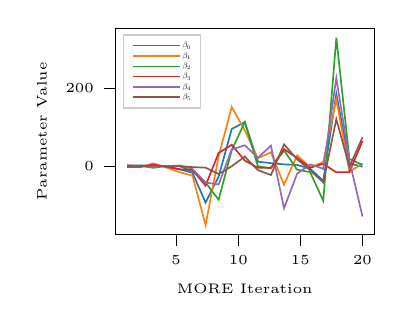
\begin{tikzpicture}

\definecolor{color0}{rgb}{0.12156862745098,0.466666666666667,0.705882352941177}
\definecolor{color1}{rgb}{1,0.498039215686275,0.0549019607843137}
\definecolor{color2}{rgb}{0.172549019607843,0.627450980392157,0.172549019607843}
\definecolor{color3}{rgb}{0.83921568627451,0.152941176470588,0.156862745098039}
\definecolor{color4}{rgb}{0.580392156862745,0.403921568627451,0.741176470588235}
\definecolor{color5}{rgb}{0.549019607843137,0.337254901960784,0.294117647058824}

\begin{axis}[
legend cell align={left},
legend style={
  fill opacity=0.8,
  draw opacity=1,
  text opacity=1,
  at={(0.03,0.97)},
  anchor=north west,
  draw=white!80!black,
  nodes={scale=0.3, transform shape}
},
height=4.2cm,
tick align=outside,
tick pos=left,
% title={LS without whitening},
x grid style={white!69.0196078431373!black},
xmin=0.105263157894737, xmax=20.9473684210526,
ticklabel style = {font=\tiny},
xlabel={\tiny MORE Iteration},
ylabel={\tiny Parameter Value},
% ylabel={\tiny parameter value},
xtick style={color=black},
y grid style={white!69.0196078431373!black},
ymin=-174.244763415887, ymax=351.999761924147,
ytick style={color=black}
]
\addplot [semithick, color0]
table {%
1.05263157894737 1.06132294723888
2.10526315789474 2.06193739819695
3.15789473684211 1.88073583639135
4.21052631578947 -0.123086283009553
5.26315789473684 -8.07620858630262
6.31578947368421 -17.0593030252393
7.36842105263158 -92.9590241843598
8.42105263157895 -26.8587655640602
9.47368421052632 94.8727821397715
10.5263157894737 112.337829573446
11.5789473684211 11.3159172204001
12.6315789473684 7.71762523100675
13.6842105263158 4.45397090742156
14.7368421052632 3.24803643790387
15.7894736842105 -6.60928495432862
16.8421052631579 -37.4795104545709
17.8947368421053 184.451583940082
18.9473684210526 6.99068247604825
20 -1.46585415702719
};
\addlegendentry{$\beta_0$}
\addplot [semithick, color1]
table {%
1.05263157894737 -0.992314117620414
2.10526315789474 -3.01314990774327
3.15789473684211 6.97978246084472
4.21052631578947 -3.46686242249737
5.26315789473684 -15.4385195628296
6.31578947368421 -24.3729399328898
7.36842105263158 -150.324557718613
8.42105263157895 25.4131163178181
9.47368421052632 151.074877150159
10.5263157894737 91.1106450835075
11.5789473684211 20.0637656430311
12.6315789473684 35.3286957225948
13.6842105263158 -47.4852217976283
14.7368421052632 27.7291797336638
15.7894736842105 -2.61087907632418
16.8421052631579 9.8894259773416
17.8947368421053 170.190330132015
18.9473684210526 -14.3804825527134
20 6.50748273849673
};
\addlegendentry{$\beta_1$}
\addplot [semithick, color2]
table {%
1.05263157894737 -2.08306644308438
2.10526315789474 1.33198284531538
3.15789473684211 -4.47590681832019
4.21052631578947 0.728904102890318
5.26315789473684 -0.0242990789144503
6.31578947368421 -13.0927089261868
7.36842105263158 -41.9204495461011
8.42105263157895 -85.6875477618256
9.47368421052632 40.456690037803
10.5263157894737 112.604643253298
11.5789473684211 -0.374250642973178
12.6315789473684 -5.50737080018894
13.6842105263158 40.0710740662349
14.7368421052632 -8.89380033218496
15.7894736842105 -15.3517937773791
16.8421052631579 -88.643722455558
17.8947368421053 328.079556226873
18.9473684210526 18.6863324064035
20 2.86476720653156
};
\addlegendentry{$\beta_2$}
\addplot [semithick, color3]
table {%
1.05263157894737 -1.36618523255821
2.10526315789474 -1.75164609748179
3.15789473684211 3.97756598366229
4.21052631578947 -1.59815536737886
5.26315789473684 -7.98327909179604
6.31578947368421 -9.76539674526244
7.36842105263158 -49.8840839358279
8.42105263157895 33.6375186411652
9.47368421052632 54.4676472894814
10.5263157894737 14.1860483339669
11.5789473684211 -4.01373690738072
12.6315789473684 -4.12863095342328
13.6842105263158 43.3396258637119
14.7368421052632 20.8801779554118
15.7894736842105 -4.18439075502474
16.8421052631579 6.03093788274091
17.8947368421053 -15.7779315076167
18.9473684210526 -15.4260914382804
20 64.1022103374432
};
\addlegendentry{$\beta_3$}
\addplot [semithick, color4]
table {%
1.05263157894737 2.75266552177
2.10526315789474 0.222631082597896
3.15789473684211 -2.66831225317667
4.21052631578947 -0.157081613253339
5.26315789473684 1.74717757967663
6.31578947368421 -7.03076201430117
7.36842105263158 -41.8997254744993
8.42105263157895 -46.7119714649756
9.47368421052632 42.7112959678472
10.5263157894737 53.1938851548008
11.5789473684211 21.4427472965738
12.6315789473684 52.1938391026262
13.6842105263158 -107.554680884685
14.7368421052632 -19.360791728667
15.7894736842105 4.40529333804277
16.8421052631579 -6.78082110704009
17.8947368421053 224.683079683236
18.9473684210526 14.5493471624127
20 -128.444231803502
};
\addlegendentry{$\beta_4$}
\addplot [semithick, color5]
table {%
1.05263157894737 0.409511212005853
2.10526315789474 -0.0998236829556997
3.15789473684211 0.971438641190439
4.21052631578947 -0.250106429020075
5.26315789473684 0.125506587151471
6.31578947368421 -2.47985362888567
7.36842105263158 -3.94108254673754
8.42105263157895 -20.142947018678
9.47368421052632 -0.266294632024777
10.5263157894737 24.1889734159118
11.5789473684211 -10.1386377753676
12.6315789473684 -22.5649113623647
13.6842105263158 55.7345330983559
14.7368421052632 17.5673205505403
15.7894736842105 -10.6102233927423
16.8421052631579 -41.5055080723722
17.8947368421053 119.908371910163
18.9473684210526 -1.67449071311621
20 72.9632198348565
};
\addlegendentry{$\beta_5$}
\end{axis}

\end{tikzpicture}
}
  \subfigure[][In Whitened Space]{% This file was created by tikzplotlib v0.9.8.
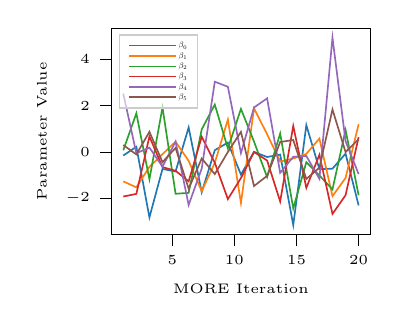
\begin{tikzpicture}

\definecolor{color0}{rgb}{0.12156862745098,0.466666666666667,0.705882352941177}
\definecolor{color1}{rgb}{1,0.498039215686275,0.0549019607843137}
\definecolor{color2}{rgb}{0.172549019607843,0.627450980392157,0.172549019607843}
\definecolor{color3}{rgb}{0.83921568627451,0.152941176470588,0.156862745098039}
\definecolor{color4}{rgb}{0.580392156862745,0.403921568627451,0.741176470588235}
\definecolor{color5}{rgb}{0.549019607843137,0.337254901960784,0.294117647058824}

\begin{axis}[
legend cell align={left},
legend style={
  fill opacity=0.6,
  draw opacity=1,
  at={(0.03,0.97)},
  anchor=north west,  
  text opacity=1,
  draw=white!80!black,
  nodes={scale=0.3, transform shape}
},
tick align=outside,
tick pos=left,
height=4.2cm,
% title={LS with whitening},
ticklabel style = {font=\tiny},
xlabel={\tiny MORE Iteration},
ylabel={\tiny Parameter Value},
% ylabel={\tiny parameter value},
x grid style={white!69.0196078431373!black},
xmin=0.105263157894737, xmax=20.9473684210526,
xtick style={color=black},
y grid style={white!69.0196078431373!black},
ymin=-3.57819481020406, ymax=5.35344627006671,
ytick style={color=black}
]
\addplot [semithick, color0]
table {%
0 nan
1.05263157894737 -0.160438320555973
2.10526315789474 0.219394431243121
3.15789473684211 -2.84098876186452
4.21052631578947 -0.740986055193629
5.26315789473684 -0.853842235649135
6.31578947368421 1.05615797377004
7.36842105263158 -1.75088534391913
8.42105263157895 0.0705918511919139
9.47368421052632 0.39885721031611
10.5263157894737 -0.985345317554263
11.5789473684211 -0.0033406902911266
12.6315789473684 -0.224957401819763
13.6842105263158 -0.120419167449998
14.7368421052632 -3.17221112473721
15.7894736842105 1.15539865077186
16.8421052631579 -0.754182051172667
17.8947368421053 -0.729231023480617
18.9473684210526 -0.0794049070163831
20 -2.32341098853369
};
\addlegendentry{$\beta_0$}
\addplot [semithick, color1]
table {%
0 nan
1.05263157894737 -1.28058969946539
2.10526315789474 -1.53894029689766
3.15789473684211 -0.652695053173459
4.21052631578947 -0.101416098811437
5.26315789473684 0.437679381326199
6.31578947368421 -0.392056022173255
7.36842105263158 -1.70729050930151
8.42105263157895 -0.476763733954958
9.47368421052632 1.39561543789549
10.5263157894737 -2.21966183479818
11.5789473684211 1.88405525337713
12.6315789473684 0.761227631336313
13.6842105263158 -0.422157877808453
14.7368421052632 -0.291442677505589
15.7894736842105 -0.0880591967377688
16.8421052631579 0.573779351363158
17.8947368421053 -1.92031146175774
18.9473684210526 -1.13217123636562
20 1.19487999215437
};
\addlegendentry{$\beta_1$}
\addplot [semithick, color2]
table {%
0 nan
1.05263157894737 0.0650603990168259
2.10526315789474 1.66692307063607
3.15789473684211 -1.19013494700324
4.21052631578947 1.92192393450495
5.26315789473684 -1.81790644534041
6.31578947368421 -1.7780930301196
7.36842105263158 0.97333460454307
8.42105263157895 2.04647534228064
9.47368421052632 0.147437818072115
10.5263157894737 1.85690654709276
11.5789473684211 0.442900159531855
12.6315789473684 -1.096945940621
13.6842105263158 0.792805164400043
14.7368421052632 -2.45161740139127
15.7894736842105 -0.44835764800036
16.8421052631579 -1.0240960807429
17.8947368421053 -1.62856319883405
18.9473684210526 0.944832473104255
20 -1.88201701337283
};
\addlegendentry{$\beta_2$}
\addplot [semithick, color3]
table {%
0 nan
1.05263157894737 -1.93676300196824
2.10526315789474 -1.82257741267246
3.15789473684211 0.663333160936527
4.21052631578947 -0.663275768747337
5.26315789473684 -0.821019212045277
6.31578947368421 -1.28113429602388
7.36842105263158 0.65291281010551
8.42105263157895 -0.472624631498625
9.47368421052632 -2.04993917968636
10.5263157894737 -1.13551165377693
11.5789473684211 -0.00633352819135336
12.6315789473684 -0.376128404445014
13.6842105263158 -2.14995102256074
14.7368421052632 1.12067150617028
15.7894736842105 -1.56239905578431
16.8421052631579 -0.127546346525872
17.8947368421053 -2.69078125503629
18.9473684210526 -1.87910414738513
20 0.635251143660584
};
\addlegendentry{$\beta_3$}
\addplot [semithick, color4]
table {%
0 nan
1.05263157894737 2.52453776967748
2.10526315789474 -0.0622806792755179
3.15789473684211 0.183127852554953
4.21052631578947 -0.641764547689705
5.26315789473684 0.443890894551663
6.31578947368421 -2.3007864289561
7.36842105263158 -0.724202884305551
8.42105263157895 3.03686607979986
9.47368421052632 2.81751806213361
10.5263157894737 -0.0549888328139704
11.5789473684211 1.91986733015714
12.6315789473684 2.31568458717932
13.6842105263158 -0.910394454807357
14.7368421052632 -0.214527507388192
15.7894736842105 -0.180563603450886
16.8421052631579 -1.17055644384447
17.8947368421053 4.94746258459985
18.9473684210526 0.461147228532594
20 -0.965335036918093
};
\addlegendentry{$\beta_4$}
\addplot [semithick, color5]
table {%
0 nan
1.05263157894737 0.294437493379665
2.10526315789474 -0.1139498169561
3.15789473684211 0.866729836873749
4.21052631578947 -0.448189417973229
5.26315789473684 0.170182259065454
6.31578947368421 -1.59646530932305
7.36842105263158 -0.289840236095353
8.42105263157895 -0.965178184382167
9.47368421052632 -0.00887931933374925
10.5263157894737 0.864473601341435
11.5789473684211 -1.48241084888596
12.6315789473684 -1.04128081547766
13.6842105263158 0.424880160759636
14.7368421052632 0.511407021464061
15.7894736842105 -1.17711053695753
16.8421052631579 -0.685355137682251
17.8947368421053 1.83511136586433
18.9473684210526 -0.0119412978270723
20 0.549279697301185
};
\addlegendentry{$\beta_5$}
\end{axis}

\end{tikzpicture}
}
  \subfigure[][Unwhitened Parameters]{% This file was created by tikzplotlib v0.9.8.
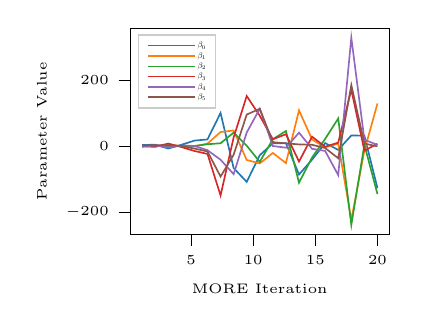
\begin{tikzpicture}

\definecolor{color0}{rgb}{0.12156862745098,0.466666666666667,0.705882352941177}
\definecolor{color1}{rgb}{1,0.498039215686275,0.0549019607843137}
\definecolor{color2}{rgb}{0.172549019607843,0.627450980392157,0.172549019607843}
\definecolor{color3}{rgb}{0.83921568627451,0.152941176470588,0.156862745098039}
\definecolor{color4}{rgb}{0.580392156862745,0.403921568627451,0.741176470588235}
\definecolor{color5}{rgb}{0.549019607843137,0.337254901960784,0.294117647058824}

\begin{axis}[
legend cell align={left},
legend style={
  fill opacity=0.8,
  draw opacity=1,
  text opacity=1,
  at={(0.03,0.97)},
  anchor=north west,
  draw=white!80!black,
  nodes={scale=0.3, transform shape}  
},
tick align=outside,
tick pos=left,
% title={LS unwhitened parameters},
height=4.2cm,
ticklabel style = {font=\tiny},
xlabel={\tiny MORE Iteration},
ylabel={\tiny Parameter Value},
% ylabel={\tiny parameter value},
x grid style={white!69.0196078431373!black},
xmin=0.105263157894737, xmax=20.9473684210526,
xtick style={color=black},
y grid style={white!69.0196078431373!black},
ymin=-268.197846135806, ymax=356.45825755095,
ytick style={color=black}
]
\addplot [semithick, color0]
table {%
0 nan
1.05263157894737 2.73237046512443
2.10526315789474 3.50329219488935
3.15789473684211 -7.95513196920218
4.21052631578947 3.1963107412616
5.26315789473684 15.9665582377668
6.31578947368421 19.5307936284837
7.36842105263158 99.7682765388784
8.42105263157895 -67.2748857277562
9.47368421052632 -108.935446206743
10.5263157894737 -28.3723498900333
11.5789473684211 8.02737185659973
12.6315789473684 8.25753374056888
13.6842105263158 -86.681775463101
14.7368421052632 -41.7602661650808
15.7894736842105 8.36880712480868
16.8421052631579 -12.0636904267509
17.8947368421053 31.5528074813332
18.9473684210526 30.8502097851426
20 -128.199402412295
};
\addlegendentry{$\beta_0$}
\addplot [semithick, color1]
table {%
0 nan
1.05263157894737 -2.75266552179048
2.10526315789474 -0.222631082543601
3.15789473684211 2.66831225443264
4.21052631578947 0.157081610925826
5.26315789473684 -1.74717757879778
6.31578947368421 7.03076202626305
7.36842105263158 41.8997530423213
8.42105263157895 46.7120202218868
9.47368421052632 -42.7113502411796
10.5263157894737 -53.1940906965109
11.5789473684211 -21.4426407071392
12.6315789473684 -52.1939970742733
13.6842105263158 107.557726652287
14.7368421052632 19.3606919269482
15.7894736842105 -4.40526650509542
16.8421052631579 6.78254399060069
17.8947368421053 -224.674204975011
18.9473684210526 -14.5477576387639
20 128.439447180318
};
\addlegendentry{$\beta_1$}
\addplot [semithick, color2]
table {%
0 nan
1.05263157894737 -0.819022424049623
2.10526315789474 0.199647365891375
3.15789473684211 -1.9428772830007
4.21052631578947 0.500212858929399
5.26315789473684 -0.251013176226387
6.31578947368421 4.9597072663002
7.36842105263158 7.88216971613495
8.42105263157895 40.2859009221452
9.47368421052632 0.532562194060467
10.5263157894737 -48.3780484798251
11.5789473684211 20.277342358223
12.6315789473684 45.129492712781
13.6842105263158 -111.472711995177
14.7368421052632 -35.1344457796991
15.7894736842105 21.2201027003383
16.8421052631579 83.0067829103594
17.8947368421053 -239.804386877317
18.9473684210526 3.34986364357253
20 -145.927381337727
};
\addlegendentry{$\beta_2$}
\addplot [semithick, color3]
table {%
0 nan
1.05263157894737 -0.992314117619856
2.10526315789474 -3.01314990781928
3.15789473684211 6.97978246214006
4.21052631578947 -3.46686242119162
5.26315789473684 -15.4385195979172
6.31578947368421 -24.3729400484366
7.36842105263158 -150.324690640714
8.42105263157895 25.4129175845349
9.47368421052632 151.075076475993
10.5263157894737 91.1111091388412
11.5789473684211 20.0637416066171
12.6315789473684 35.3285999194684
13.6842105263158 -47.4864678609504
14.7368421052632 27.7291529085892
15.7894736842105 -2.6109304150866
16.8421052631579 9.88947690188812
17.8947368421053 170.184421049193
18.9473684210526 -14.380534116013
20 6.50803958125695
};
\addlegendentry{$\beta_3$}
\addplot [semithick, color4]
table {%
0 nan
1.05263157894737 -2.08306644313421
2.10526315789474 1.33198284534283
3.15789473684211 -4.47590681922109
4.21052631578947 0.728904102368964
5.26315789473684 -0.0242990829679821
6.31578947368421 -13.0927089380793
7.36842105263158 -41.9204793443672
8.42105263157895 -85.6876009016413
9.47368421052632 40.4567691407284
10.5263157894737 112.604939441663
11.5789473684211 -0.374362345187074
12.6315789473684 -5.50699678442577
13.6842105263158 40.0725752199367
14.7368421052632 -8.89380637913888
15.7894736842105 -15.351529102298
16.8421052631579 -88.6413918339742
17.8947368421053 328.064798292462
18.9473684210526 18.6842293882621
20 2.86800939663844
};
\addlegendentry{$\beta_4$}
\addplot [semithick, color5]
table {%
0 nan
1.05263157894737 1.06132294724826
2.10526315789474 2.0619373982425
3.15789473684211 1.88073583669649
4.21052631578947 -0.123086282337559
5.26315789473684 -8.07620859625119
6.31578947368421 -17.0593030680154
7.36842105263158 -92.9591020970872
8.42105263157895 -26.8588894445826
9.47368421052632 94.8729166288909
10.5263157894737 112.33820540046
11.5789473684211 11.3158701183703
12.6315789473684 7.71772676655036
13.6842105263158 4.45426808265695
14.7368421052632 3.24805664772185
15.7894736842105 -6.60919932524989
16.8421052631579 -37.4784670914881
17.8947368421053 184.443910566116
18.9473684210526 6.98961781772105
20 -1.46457078349287
};
\addlegendentry{$\beta_5$}
\end{axis}

\end{tikzpicture}
}
  \caption{\small
    Example of using MORE with a least squares approach for
    surrogate-modeling with and without whitening on the 2-dimensional
    Rosenbrock function (\Cref{sec:test_func}).
    The plots show the predicted surrogate model
    parameters $\mathbf{\beta}$. In (a) the parameters are estimated
    without whitening the data. In (b) a whitening transformation is
    applied to the data before parameter estimation
    and (c) shows the parameters from (b) after reversing
    the whitening transformation.
    We can see that the parameters in whitened space
    stay in a smaller range 
    making the estimation task easier.}
 \label{fig:whitening}
\end{figure}


\section{MORE with Recursive Surrogate-Modeling}
We now present the MORE algorithm with recursive surrogate-modeling.
First we initialize the search distribution 
$\pi(\mathbf{x}) = \mathcal{N}(\mathbf{x} |\, \mu, \Sigma)$ and
the RLS algorithm. In the robot
learning setting the search distribution may be initialized
through imitation learning.
In each iteration the search distribution is then used to create
samples which are evaluated on the objective function.
The samples are used to create the design matrix $\mathbf{X}$
(as in \ref{eq:lgs}).
Data preprocessing techniques like whitening (\Cref{sec:whitening})
and normalization
may be applied to the design matrix and rewards before they
are given to the RLS algorithm to learn the surrogate model, which in turn
is used to compute the update to the search distribution in closed form.
MORE with Recursive Surrogate-Modeling is summarized in \Cref{alg:more}.

\begin{algorithm}[H]
\renewcommand{\algorithmcfname}{Algorithm}
\DontPrintSemicolon
\SetAlgoLined
\KwIn{Parameters $\epsilon$ and $\beta$, \\ $K$ number of iterations,
  $N$ samples per iteration}
\Begin(Initialization:)
{
  Initialize search distribution $\pi$ \;
  Initialize RLS with $\mathbf{m}_0, \mathbf{P}_0$ \;
}
\For{$k = 1,...,K$}
{
  \For{$n = 1,...,N$}
  {
    Draw sample $\mathbf{x}_n \sim \pi$\;
    Evaluate $\mathbf{x}_n$ on objective function $f(\mathbf{x}_n) = y_n$\;
  }
  \Begin(Estimate quadratic model $\hat{f}$)
  {
    \For{$n = 1,...,N$}
    {
      Whitening: $\mathbf{X}_n = \mathbf{W} \, \mathbf{X}_n$\;
      % TODO: normalization maybe in fundamentals
      % Optionally: Use normalization\;
      Optionally: Increase model noise for older samples\;      
      Compute surrogate model parameters using \Cref{RLS:basic} \;
      % RLS$(\mathbf{X}_n, y_n, \mathbf{Q}, \sigma^2)$ \;
    }
  }
  Solve  $\text{argmin}_{\eta >0, \omega > 0} \, g(\eta, \omega)$
  using \Cref{eq:dual} \;
  Update search distribution $\pi$ using \Cref{policy_update}\;
}
\caption{MORE with Recursive Surrogate-Modeling}
\label{alg:more}
\end{algorithm}

%\subsection{Moving back to prior}
%One technique we investigated is 
%- to prior calculation (optimal for whitened space)
%
%- set up equation
%
%\subsection{State Transition Model}
%Let us quickly state the full Kalman filter equations, the
%derivation can be found in the appendix (TODO ref)
%
%Prediction step:
%
%Update step:
%
%Introducing an accurate state transition model to incorporate the
%prediction step of the kalman filter would be ideal.
%We tried some simple momentum approaches based on the differences of
%subsequent surrogate model parameters, but those did not yield
%good results.
%Our Recursive least squares algorithm is a special case of these
%equations using an state transition model matrix $\mathbf{A} = \mathbf{I}$.
%